\documentclass[a4paper]{book}
\usepackage{makeidx}
\usepackage{graphicx}
\usepackage{multicol}
\usepackage{float}
\usepackage{listings}
\usepackage{color}
\usepackage{textcomp}
\usepackage{alltt}
\usepackage{times}
\usepackage{ifpdf}
\ifpdf
\usepackage[pdftex,
            pagebackref=true,
            colorlinks=true,
            linkcolor=blue,
            unicode
           ]{hyperref}
\else
\usepackage[ps2pdf,
            pagebackref=true,
            colorlinks=true,
            linkcolor=blue,
            unicode
           ]{hyperref}
\usepackage{pspicture}
\fi
\usepackage[utf8]{inputenc}
\usepackage{doxygen}
\lstset{language=C++,inputencoding=utf8,basicstyle=\footnotesize,breaklines=true,breakatwhitespace=true,tabsize=8,numbers=left }
\makeindex
\setcounter{tocdepth}{3}
\renewcommand{\footrulewidth}{0.4pt}
\begin{document}
\hypersetup{pageanchor=false}
\begin{titlepage}
\vspace*{7cm}
\begin{center}
{\Large Rleg \\[1ex]\large 2 }\\
\vspace*{1cm}
{\large Generated by Doxygen 1.6.3}\\
\vspace*{0.5cm}
{\small Wed Dec 4 12:19:21 2013}\\
\end{center}
\end{titlepage}
\clearemptydoublepage
\pagenumbering{roman}
\tableofcontents
\clearemptydoublepage
\pagenumbering{arabic}
\hypersetup{pageanchor=true}
\chapter{Todo List}
\label{todo}
\hypertarget{todo}{}

\begin{DoxyRefList}
\item[\label{todo__todo000002}%
\hypertarget{todo__todo000002}{}%
Global \hyperlink{group__gyr_gad817a3b69d4c3026b7a9b6de32753e7b}{gyr\-\_\-read\-\_\-reg} (int i2c\-\_\-dev, uint8\-\_\-t reg, uint8\-\_\-t count)]Verify use of reg parameter  
\item[\label{todo__todo000001}%
\hypertarget{todo__todo000001}{}%
Global \hyperlink{communication_2communication_8h_a8da2a9706cfdbe1a7fae96aac9e4f516}{mra\-\_\-shut\-\_\-down} (void)]Check this function 
\end{DoxyRefList}
\chapter{Module Index}
\section{Modules}
Here is a list of all modules\-:\begin{DoxyCompactList}
\item \contentsline{section}{Function of Encoder A\-M\-T203}{\pageref{group__enc}}{}
\item \contentsline{section}{Functions for accelerometer A\-D\-X\-L345}{\pageref{group__acc}}{}
\item \contentsline{section}{Functions for Gyrometer I\-T\-G3200}{\pageref{group__gyr}}{}
\item \contentsline{section}{Functions to Magnetometer H\-M\-C5883}{\pageref{group__mag}}{}
\item \contentsline{section}{Functions to deal the User Inteface using ncurses}{\pageref{group__ui}}{}
\end{DoxyCompactList}

\chapter{Data Structure Index}
\section{Data Structures}
Here are the data structures with brief descriptions\-:\begin{DoxyCompactList}
\item\contentsline{section}{\hyperlink{structIMU__DATA__STRUCT_1_1calibrated}{I\-M\-U\-\_\-\-D\-A\-T\-A\-\_\-\-S\-T\-R\-U\-C\-T\-::calibrated} }{\pageref{structIMU__DATA__STRUCT_1_1calibrated}}{}
\item\contentsline{section}{\hyperlink{classCartesian__controller}{Cartesian\-\_\-controller} }{\pageref{classCartesian__controller}}{}
\item\contentsline{section}{\hyperlink{classCartesian__pose__controller}{Cartesian\-\_\-pose\-\_\-controller} }{\pageref{classCartesian__pose__controller}}{}
\item\contentsline{section}{\hyperlink{classCartesian__velocity__controller}{Cartesian\-\_\-velocity\-\_\-controller} }{\pageref{classCartesian__velocity__controller}}{}
\item\contentsline{section}{\hyperlink{structDATA__XYZ}{D\-A\-T\-A\-\_\-\-X\-Y\-Z} \\*A structure to represent a 3d Vector }{\pageref{structDATA__XYZ}}{}
\item\contentsline{section}{\hyperlink{structDATA__XYZ__DOUBLE}{D\-A\-T\-A\-\_\-\-X\-Y\-Z\-\_\-\-D\-O\-U\-B\-L\-E} \\*Vector definition on double }{\pageref{structDATA__XYZ__DOUBLE}}{}
\item\contentsline{section}{\hyperlink{structDQ}{D\-Q} \\*Dual\-Quaternion library Header }{\pageref{structDQ}}{}
\item\contentsline{section}{\hyperlink{structDUMMY__MATRICES}{D\-U\-M\-M\-Y\-\_\-\-M\-A\-T\-R\-I\-C\-E\-S} }{\pageref{structDUMMY__MATRICES}}{}
\item\contentsline{section}{\hyperlink{structEFF__DATA__STRUCT}{E\-F\-F\-\_\-\-D\-A\-T\-A\-\_\-\-S\-T\-R\-U\-C\-T} }{\pageref{structEFF__DATA__STRUCT}}{}
\item\contentsline{section}{\hyperlink{structGDATALOGGER}{G\-D\-A\-T\-A\-L\-O\-G\-G\-E\-R} }{\pageref{structGDATALOGGER}}{}
\item\contentsline{section}{\hyperlink{structGDATALOGGERIPC__SHM}{G\-D\-A\-T\-A\-L\-O\-G\-G\-E\-R\-I\-P\-C\-\_\-\-S\-H\-M} }{\pageref{structGDATALOGGERIPC__SHM}}{}
\item\contentsline{section}{\hyperlink{structGDATALOGGERVARIABLE}{G\-D\-A\-T\-A\-L\-O\-G\-G\-E\-R\-V\-A\-R\-I\-A\-B\-L\-E} }{\pageref{structGDATALOGGERVARIABLE}}{}
\item\contentsline{section}{\hyperlink{structGMATLABDATAFILECONFIG}{G\-M\-A\-T\-L\-A\-B\-D\-A\-T\-A\-F\-I\-L\-E\-C\-O\-N\-F\-I\-G} }{\pageref{structGMATLABDATAFILECONFIG}}{}
\item\contentsline{section}{\hyperlink{structGMATRIX}{G\-M\-A\-T\-R\-I\-X} }{\pageref{structGMATRIX}}{}
\item\contentsline{section}{\hyperlink{structGMATRIX__MATLAB__DATAHEAD}{G\-M\-A\-T\-R\-I\-X\-\_\-\-M\-A\-T\-L\-A\-B\-\_\-\-D\-A\-T\-A\-H\-E\-A\-D} }{\pageref{structGMATRIX__MATLAB__DATAHEAD}}{}
\item\contentsline{section}{\hyperlink{structGQUEUECONTROL}{G\-Q\-U\-E\-U\-E\-C\-O\-N\-T\-R\-O\-L} }{\pageref{structGQUEUECONTROL}}{}
\item\contentsline{section}{\hyperlink{structIMU__DATA__STRUCT}{I\-M\-U\-\_\-\-D\-A\-T\-A\-\_\-\-S\-T\-R\-U\-C\-T} \\*Data of I\-M\-U structure }{\pageref{structIMU__DATA__STRUCT}}{}
\item\contentsline{section}{\hyperlink{structIMU__PARAM__STRUCT}{I\-M\-U\-\_\-\-P\-A\-R\-A\-M\-\_\-\-S\-T\-R\-U\-C\-T} \\*Configs of I\-M\-U }{\pageref{structIMU__PARAM__STRUCT}}{}
\item\contentsline{section}{\hyperlink{structLink}{Link} }{\pageref{structLink}}{}
\item\contentsline{section}{\hyperlink{structMATLAB__DATAHEAD}{M\-A\-T\-L\-A\-B\-\_\-\-D\-A\-T\-A\-H\-E\-A\-D} }{\pageref{structMATLAB__DATAHEAD}}{}
\item\contentsline{section}{\hyperlink{classMatrix}{Matrix} }{\pageref{classMatrix}}{}
\item\contentsline{section}{\hyperlink{structMRA__DATA__STRUCT}{M\-R\-A\-\_\-\-D\-A\-T\-A\-\_\-\-S\-T\-R\-U\-C\-T} \\*Struct to control M\-R\-A }{\pageref{structMRA__DATA__STRUCT}}{}
\item\contentsline{section}{\hyperlink{structIMU__PARAM__STRUCT_1_1param__acc}{I\-M\-U\-\_\-\-P\-A\-R\-A\-M\-\_\-\-S\-T\-R\-U\-C\-T\-::param\-\_\-acc} \\*Accelerometer Parameters }{\pageref{structIMU__PARAM__STRUCT_1_1param__acc}}{}
\item\contentsline{section}{\hyperlink{structIMU__PARAM__STRUCT_1_1param__gyr}{I\-M\-U\-\_\-\-P\-A\-R\-A\-M\-\_\-\-S\-T\-R\-U\-C\-T\-::param\-\_\-gyr} \\*Gyrometer Parameters }{\pageref{structIMU__PARAM__STRUCT_1_1param__gyr}}{}
\item\contentsline{section}{\hyperlink{structIMU__PARAM__STRUCT_1_1param__mag}{I\-M\-U\-\_\-\-P\-A\-R\-A\-M\-\_\-\-S\-T\-R\-U\-C\-T\-::param\-\_\-mag} \\*Magnetometer Parameters }{\pageref{structIMU__PARAM__STRUCT_1_1param__mag}}{}
\item\contentsline{section}{\hyperlink{structQ}{Q} }{\pageref{structQ}}{}
\item\contentsline{section}{\hyperlink{structRobot}{Robot} \\*The Structure holding the relevant info of a \hyperlink{structRobot}{Robot} }{\pageref{structRobot}}{}
\item\contentsline{section}{\hyperlink{structSPI__PARAM__STRUCT}{S\-P\-I\-\_\-\-P\-A\-R\-A\-M\-\_\-\-S\-T\-R\-U\-C\-T} \\*Configs for S\-P\-I }{\pageref{structSPI__PARAM__STRUCT}}{}
\end{DoxyCompactList}

\chapter{File Index}
\section{File List}
Here is a list of all files with brief descriptions\-:\begin{DoxyCompactList}
\item\contentsline{section}{\hyperlink{calibration_8c}{calibration.\-c} }{\pageref{calibration_8c}}{}
\item\contentsline{section}{\hyperlink{calibration_8h}{calibration.\-h} }{\pageref{calibration_8h}}{}
\item\contentsline{section}{\hyperlink{datalogger_8c}{datalogger.\-c} }{\pageref{datalogger_8c}}{}
\item\contentsline{section}{\hyperlink{datalogger_8h}{datalogger.\-h} }{\pageref{datalogger_8h}}{}
\item\contentsline{section}{\hyperlink{main_8c}{main.\-c} }{\pageref{main_8c}}{}
\item\contentsline{section}{\hyperlink{main_8h}{main.\-h} }{\pageref{main_8h}}{}
\item\contentsline{section}{\hyperlink{main2_8c}{main2.\-c} }{\pageref{main2_8c}}{}
\item\contentsline{section}{\hyperlink{main2_8h}{main2.\-h} }{\pageref{main2_8h}}{}
\item\contentsline{section}{\hyperlink{threads__linux_8c}{threads\-\_\-linux.\-c} }{\pageref{threads__linux_8c}}{}
\item\contentsline{section}{\hyperlink{ui_8c}{ui.\-c} }{\pageref{ui_8c}}{}
\item\contentsline{section}{\hyperlink{ui_8h}{ui.\-h} }{\pageref{ui_8h}}{}
\item\contentsline{section}{calibration/\hyperlink{calibration_2calibration_8c}{calibration.\-c} }{\pageref{calibration_2calibration_8c}}{}
\item\contentsline{section}{calibration/\hyperlink{calibration_2calibration_8h}{calibration.\-h} }{\pageref{calibration_2calibration_8h}}{}
\item\contentsline{section}{communication/\hyperlink{communication_2acc__functions_8c}{acc\-\_\-functions.\-c} }{\pageref{communication_2acc__functions_8c}}{}
\item\contentsline{section}{communication/\hyperlink{communication_01_07C_xC3_xB3pia_01em_01conflito_01de_01Caio_01Gustavo_01Mesquita_01Angelo_012013-05-17_08_8c}{communication (\-Cópia em conflito de Caio Gustavo Mesquita Angelo 2013-\/05-\/17).\-c} }{\pageref{communication_01_07C_xC3_xB3pia_01em_01conflito_01de_01Caio_01Gustavo_01Mesquita_01Angelo_012013-05-17_08_8c}}{}
\item\contentsline{section}{communication/\hyperlink{communication_01_07C_xC3_xB3pia_01em_01conflito_01de_01Caio_01Gustavo_01Mesquita_01Angelo_012013-05-17_08_8h}{communication (\-Cópia em conflito de Caio Gustavo Mesquita Angelo 2013-\/05-\/17).\-h} }{\pageref{communication_01_07C_xC3_xB3pia_01em_01conflito_01de_01Caio_01Gustavo_01Mesquita_01Angelo_012013-05-17_08_8h}}{}
\item\contentsline{section}{communication/\hyperlink{communication_2communication_8c}{communication.\-c} }{\pageref{communication_2communication_8c}}{}
\item\contentsline{section}{communication/\hyperlink{communication_2communication_8h}{communication.\-h} }{\pageref{communication_2communication_8h}}{}
\item\contentsline{section}{communication/\hyperlink{communication_2gpio__functions_8c}{gpio\-\_\-functions.\-c} }{\pageref{communication_2gpio__functions_8c}}{}
\item\contentsline{section}{communication/\hyperlink{communication_2gpio__functions_8h}{gpio\-\_\-functions.\-h} }{\pageref{communication_2gpio__functions_8h}}{}
\item\contentsline{section}{communication/\hyperlink{communication_2gyr__functions_8c}{gyr\-\_\-functions.\-c} }{\pageref{communication_2gyr__functions_8c}}{}
\item\contentsline{section}{communication/\hyperlink{communication_2imu__functions_8h}{imu\-\_\-functions.\-h} }{\pageref{communication_2imu__functions_8h}}{}
\item\contentsline{section}{communication/\hyperlink{communication_2imu__regs_8h}{imu\-\_\-regs.\-h} }{\pageref{communication_2imu__regs_8h}}{}
\item\contentsline{section}{communication/\hyperlink{communication_2mag__functions_8c}{mag\-\_\-functions.\-c} }{\pageref{communication_2mag__functions_8c}}{}
\item\contentsline{section}{communication/\hyperlink{communication_2spi__functions_8c}{spi\-\_\-functions.\-c} }{\pageref{communication_2spi__functions_8c}}{}
\item\contentsline{section}{communication/\hyperlink{communication_2spi__functions_8h}{spi\-\_\-functions.\-h} }{\pageref{communication_2spi__functions_8h}}{}
\item\contentsline{section}{Communication\-V0/\hyperlink{CommunicationV0_2acc__functions_8c}{acc\-\_\-functions.\-c} }{\pageref{CommunicationV0_2acc__functions_8c}}{}
\item\contentsline{section}{Communication\-V0/\hyperlink{CommunicationV0_2communication_8c}{communication.\-c} }{\pageref{CommunicationV0_2communication_8c}}{}
\item\contentsline{section}{Communication\-V0/\hyperlink{CommunicationV0_2communication_8h}{communication.\-h} }{\pageref{CommunicationV0_2communication_8h}}{}
\item\contentsline{section}{Communication\-V0/\hyperlink{CommunicationV0_2gpio__functions_8c}{gpio\-\_\-functions.\-c} }{\pageref{CommunicationV0_2gpio__functions_8c}}{}
\item\contentsline{section}{Communication\-V0/\hyperlink{CommunicationV0_2gpio__functions_8h}{gpio\-\_\-functions.\-h} }{\pageref{CommunicationV0_2gpio__functions_8h}}{}
\item\contentsline{section}{Communication\-V0/\hyperlink{CommunicationV0_2gyr__functions_8c}{gyr\-\_\-functions.\-c} }{\pageref{CommunicationV0_2gyr__functions_8c}}{}
\item\contentsline{section}{Communication\-V0/\hyperlink{CommunicationV0_2imu__functions_8h}{imu\-\_\-functions.\-h} }{\pageref{CommunicationV0_2imu__functions_8h}}{}
\item\contentsline{section}{Communication\-V0/\hyperlink{CommunicationV0_2imu__regs_8h}{imu\-\_\-regs.\-h} }{\pageref{CommunicationV0_2imu__regs_8h}}{}
\item\contentsline{section}{Communication\-V0/\hyperlink{CommunicationV0_2mag__functions_8c}{mag\-\_\-functions.\-c} }{\pageref{CommunicationV0_2mag__functions_8c}}{}
\item\contentsline{section}{Communication\-V0/\hyperlink{CommunicationV0_2spi__functions_8c}{spi\-\_\-functions.\-c} }{\pageref{CommunicationV0_2spi__functions_8c}}{}
\item\contentsline{section}{Communication\-V0/\hyperlink{CommunicationV0_2spi__functions_8h}{spi\-\_\-functions.\-h} }{\pageref{CommunicationV0_2spi__functions_8h}}{}
\item\contentsline{section}{control/\hyperlink{control_8c}{control.\-c} }{\pageref{control_8c}}{}
\item\contentsline{section}{gdatalogger/\hyperlink{gdatalogger_8c}{gdatalogger.\-c} }{\pageref{gdatalogger_8c}}{}
\item\contentsline{section}{gdatalogger/\hyperlink{gdatalogger_8h}{gdatalogger.\-h} }{\pageref{gdatalogger_8h}}{}
\item\contentsline{section}{gdatalogger/\hyperlink{gmatlabdatafile_8c}{gmatlabdatafile.\-c} }{\pageref{gmatlabdatafile_8c}}{}
\item\contentsline{section}{gdatalogger/\hyperlink{gmatlabdatafile_8h}{gmatlabdatafile.\-h} }{\pageref{gmatlabdatafile_8h}}{}
\item\contentsline{section}{gdatalogger/\hyperlink{gqueue_8c}{gqueue.\-c} }{\pageref{gqueue_8c}}{}
\item\contentsline{section}{gdatalogger/\hyperlink{gqueue_8h}{gqueue.\-h} }{\pageref{gqueue_8h}}{}
\item\contentsline{section}{schunk\-\_\-high/include/schunk\-\_\-high/\hyperlink{cartesian__controller_8h}{cartesian\-\_\-controller.\-h} }{\pageref{cartesian__controller_8h}}{}
\item\contentsline{section}{schunk\-\_\-high/include/schunk\-\_\-high/\hyperlink{cartesian__pose__controller_8h}{cartesian\-\_\-pose\-\_\-controller.\-h} }{\pageref{cartesian__pose__controller_8h}}{}
\item\contentsline{section}{schunk\-\_\-high/include/schunk\-\_\-high/\hyperlink{cartesian__velocity__controller_8h}{cartesian\-\_\-velocity\-\_\-controller.\-h} }{\pageref{cartesian__velocity__controller_8h}}{}
\item\contentsline{section}{schunk\-\_\-high/include/schunk\-\_\-high/\hyperlink{dualquaternion_8h}{dualquaternion.\-h} }{\pageref{dualquaternion_8h}}{}
\item\contentsline{section}{schunk\-\_\-high/include/schunk\-\_\-high/\hyperlink{gmatrix_8h}{gmatrix.\-h} }{\pageref{gmatrix_8h}}{}
\item\contentsline{section}{schunk\-\_\-high/include/schunk\-\_\-high/\hyperlink{gmatrix__linalg_8h}{gmatrix\-\_\-linalg.\-h} }{\pageref{gmatrix__linalg_8h}}{}
\item\contentsline{section}{schunk\-\_\-high/include/schunk\-\_\-high/\hyperlink{gmatrix__plus_8h}{gmatrix\-\_\-plus.\-h} }{\pageref{gmatrix__plus_8h}}{}
\item\contentsline{section}{schunk\-\_\-high/include/schunk\-\_\-high/\hyperlink{link_8h}{link.\-h} }{\pageref{link_8h}}{}
\item\contentsline{section}{schunk\-\_\-high/include/schunk\-\_\-high/\hyperlink{quaternion_8h}{quaternion.\-h} }{\pageref{quaternion_8h}}{}
\item\contentsline{section}{schunk\-\_\-high/include/schunk\-\_\-high/\hyperlink{robot_8h}{robot.\-h} }{\pageref{robot_8h}}{}
\item\contentsline{section}{schunk\-\_\-high/src/\hyperlink{cartesian__controller_8cpp}{cartesian\-\_\-controller.\-cpp} }{\pageref{cartesian__controller_8cpp}}{}
\item\contentsline{section}{schunk\-\_\-high/src/\hyperlink{cartesian__pose__controller_8cpp}{cartesian\-\_\-pose\-\_\-controller.\-cpp} }{\pageref{cartesian__pose__controller_8cpp}}{}
\item\contentsline{section}{schunk\-\_\-high/src/\hyperlink{cartesian__velocity__controller_8cpp}{cartesian\-\_\-velocity\-\_\-controller.\-cpp} }{\pageref{cartesian__velocity__controller_8cpp}}{}
\item\contentsline{section}{schunk\-\_\-high/src/\hyperlink{schunk__high_8cpp}{schunk\-\_\-high.\-cpp} }{\pageref{schunk__high_8cpp}}{}
\item\contentsline{section}{schunk\-\_\-high/src/kinematics/\hyperlink{link_8c}{link.\-c} }{\pageref{link_8c}}{}
\item\contentsline{section}{schunk\-\_\-high/src/kinematics/\hyperlink{robot_8c}{robot.\-c} }{\pageref{robot_8c}}{}
\item\contentsline{section}{schunk\-\_\-high/src/matrix/\hyperlink{gmatrix_8c}{gmatrix.\-c} }{\pageref{gmatrix_8c}}{}
\item\contentsline{section}{schunk\-\_\-high/src/matrix/\hyperlink{gmatrix__linalg_8c}{gmatrix\-\_\-linalg.\-c} }{\pageref{gmatrix__linalg_8c}}{}
\item\contentsline{section}{schunk\-\_\-high/src/matrix/\hyperlink{gmatrix__plus_8c}{gmatrix\-\_\-plus.\-c} }{\pageref{gmatrix__plus_8c}}{}
\item\contentsline{section}{schunk\-\_\-high/src/matrix/\hyperlink{matrix__interface_8cpp}{matrix\-\_\-interface.\-cpp} }{\pageref{matrix__interface_8cpp}}{}
\item\contentsline{section}{schunk\-\_\-high/src/quaternion/\hyperlink{dualquaternion_8c}{dualquaternion.\-c} }{\pageref{dualquaternion_8c}}{}
\item\contentsline{section}{schunk\-\_\-high/src/quaternion/\hyperlink{quaternion_8c}{quaternion.\-c} }{\pageref{quaternion_8c}}{}
\end{DoxyCompactList}

\chapter{Module Documentation}
\hypertarget{group__calibrate}{\section{Routines to calibrate sensors}
\label{group__calibrate}\index{Routines to calibrate sensors@{Routines to calibrate sensors}}
}
Collaboration diagram for Routines to calibrate sensors\-:
\nopagebreak
\begin{figure}[H]
\begin{center}
\leavevmode
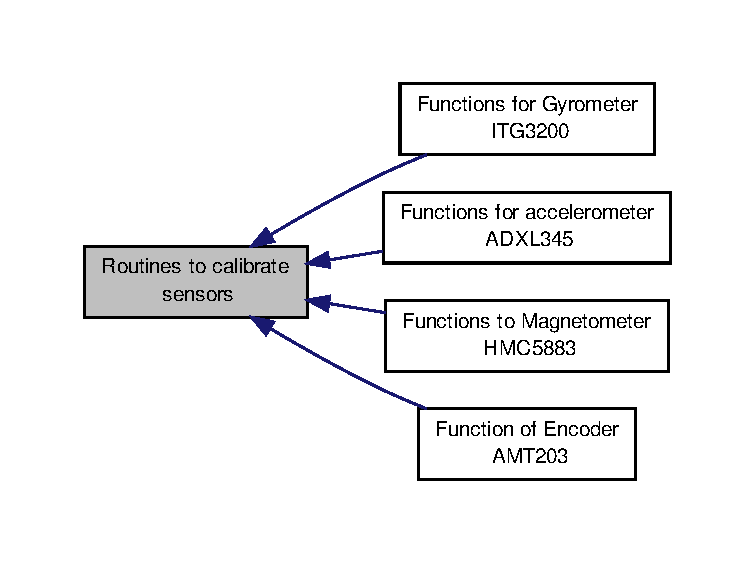
\includegraphics[width=350pt]{group__calibrate}
\end{center}
\end{figure}
\subsection*{Modules}
\begin{DoxyCompactItemize}
\item 
\hyperlink{group__acc}{Functions for accelerometer A\-D\-X\-L345}
\item 
\hyperlink{group__mag}{Functions to Magnetometer H\-M\-C5883}
\item 
\hyperlink{group__gyr}{Functions for Gyrometer I\-T\-G3200}
\item 
\hyperlink{group__enc}{Function of Encoder A\-M\-T203}
\end{DoxyCompactItemize}
\subsection*{Functions}
\begin{DoxyCompactItemize}
\item 
void \hyperlink{group__calibrate_ga043045246cf217758281222214c4addc}{calibrate\-\_\-all} (\hyperlink{structIMU__DATA__STRUCT}{I\-M\-U\-\_\-\-D\-A\-T\-A\-\_\-\-S\-T\-R\-U\-C\-T} $\ast$\hyperlink{threads__linux_8c_a3cfea12cbe9ca7f1681c950e4cd68606}{imu\-\_\-data})
\begin{DoxyCompactList}\small\item\em Calibrate all sensors. \end{DoxyCompactList}\item 
void \hyperlink{group__calibrate_gaecfc81d152db2843b5d1517729804d63}{calibrate\-\_\-imu} (\hyperlink{structIMU__DATA__STRUCT}{I\-M\-U\-\_\-\-D\-A\-T\-A\-\_\-\-S\-T\-R\-U\-C\-T} $\ast$\hyperlink{threads__linux_8c_a3cfea12cbe9ca7f1681c950e4cd68606}{imu\-\_\-data})
\begin{DoxyCompactList}\small\item\em Calibrate imu sensors. \end{DoxyCompactList}\item 
void \hyperlink{group__calibrate_gae8f1281c6870b23c1c158b30998f7568}{calibrate\-\_\-enc} (\hyperlink{structENC__DATA__STRUCT}{E\-N\-C\-\_\-\-D\-A\-T\-A\-\_\-\-S\-T\-R\-U\-C\-T} $\ast$\hyperlink{main2_8c_aaa441e18ae805c4f3efb0b5231d1cfe7}{enc\-\_\-data})
\begin{DoxyCompactList}\small\item\em Calibrate encoder. \end{DoxyCompactList}\end{DoxyCompactItemize}


\subsection{Detailed Description}


\subsection{Function Documentation}
\hypertarget{group__calibrate_ga043045246cf217758281222214c4addc}{\index{Routines to calibrate sensors@{Routines to calibrate sensors}!calibrate\-\_\-all@{calibrate\-\_\-all}}
\index{calibrate\-\_\-all@{calibrate\-\_\-all}!Routines to calibrate sensors@{Routines to calibrate sensors}}
\subsubsection[{calibrate\-\_\-all}]{\setlength{\rightskip}{0pt plus 5cm}void calibrate\-\_\-all (
\begin{DoxyParamCaption}
\item[{{\bf I\-M\-U\-\_\-\-D\-A\-T\-A\-\_\-\-S\-T\-R\-U\-C\-T} $\ast$}]{imu\-\_\-data}
\end{DoxyParamCaption}
)}}\label{group__calibrate_ga043045246cf217758281222214c4addc}


Calibrate all sensors. 



Definition at line 8 of file calibration.\-c.


\begin{DoxyCode}
\{
  \hyperlink{group__calibrate_gaecfc81d152db2843b5d1517729804d63}{calibrate\_imu}(imu\_data);
  \textcolor{keywordflow}{return};
\}
\end{DoxyCode}
\hypertarget{group__calibrate_gae8f1281c6870b23c1c158b30998f7568}{\index{Routines to calibrate sensors@{Routines to calibrate sensors}!calibrate\-\_\-enc@{calibrate\-\_\-enc}}
\index{calibrate\-\_\-enc@{calibrate\-\_\-enc}!Routines to calibrate sensors@{Routines to calibrate sensors}}
\subsubsection[{calibrate\-\_\-enc}]{\setlength{\rightskip}{0pt plus 5cm}void calibrate\-\_\-enc (
\begin{DoxyParamCaption}
\item[{{\bf E\-N\-C\-\_\-\-D\-A\-T\-A\-\_\-\-S\-T\-R\-U\-C\-T} $\ast$}]{enc\-\_\-data}
\end{DoxyParamCaption}
)}}\label{group__calibrate_gae8f1281c6870b23c1c158b30998f7568}


Calibrate encoder. 



Definition at line 33 of file calibration.\-c.



References E\-N\-C\-\_\-\-D\-A\-T\-A\-\_\-\-S\-T\-R\-U\-C\-T\-::angle, E\-N\-C\-\_\-\-D\-A\-T\-A\-\_\-\-S\-T\-R\-U\-C\-T\-::calibrate\-::angle, E\-N\-C\-\_\-\-D\-A\-T\-A\-\_\-\-S\-T\-R\-U\-C\-T\-::calib, and E\-N\-C\-\_\-\-F\-S.


\begin{DoxyCode}
                                             \{
  enc\_data->\hyperlink{structENC__DATA__STRUCT_af227e5bbb714b830cc570432bda0a468}{calib}.\hyperlink{structENC__DATA__STRUCT_1_1calibrate_a862c7101db8c6dbc9213857b6bc1971b}{angle} = enc\_data->\hyperlink{structENC__DATA__STRUCT_ad25beb30fd5b975292f87db02ec9930a}{angle}/\hyperlink{group__enc_gadf9edcc7e266ed7333f7570965f5956a}{ENC\_FS};
\}
\end{DoxyCode}
\hypertarget{group__calibrate_gaecfc81d152db2843b5d1517729804d63}{\index{Routines to calibrate sensors@{Routines to calibrate sensors}!calibrate\-\_\-imu@{calibrate\-\_\-imu}}
\index{calibrate\-\_\-imu@{calibrate\-\_\-imu}!Routines to calibrate sensors@{Routines to calibrate sensors}}
\subsubsection[{calibrate\-\_\-imu}]{\setlength{\rightskip}{0pt plus 5cm}void calibrate\-\_\-imu (
\begin{DoxyParamCaption}
\item[{{\bf I\-M\-U\-\_\-\-D\-A\-T\-A\-\_\-\-S\-T\-R\-U\-C\-T} $\ast$}]{imu\-\_\-data}
\end{DoxyParamCaption}
)}}\label{group__calibrate_gaecfc81d152db2843b5d1517729804d63}


Calibrate imu sensors. 



Definition at line 14 of file calibration.\-c.


\begin{DoxyCode}
\{
  \textcolor{comment}{// With this parameters, the vectors of acceleration and magnetic field will
       have norm = 1 theorically (i.e. in g or G)}
  imu\_data->\hyperlink{structIMU__DATA__STRUCT_aeffe3c3c5a7191a5cef16e7aab6c3795}{calib}.\hyperlink{structIMU__DATA__STRUCT_1_1calibrated_a281a7fdb40a05ed97388f18b9bb90c81}{acc}.\hyperlink{structDATA__XYZ__DOUBLE_a22868cc99a423900e7b82d015a5eb91f}{x} = ((double)imu\_data->\hyperlink{structIMU__DATA__STRUCT_a448f284bf44eb503affda586ad5fa9d2}{acc}.\hyperlink{structDATA__XYZ_a54c1596e9f9969fd9c21e8458024ecfb}{x}-\hyperlink{group__acc_ga355ea8f6ceed1e1d419a3ea2271bfca3}{ACC\_BIAS\_X}
      )/\hyperlink{group__acc_ga76e6967cb5a86ec34986b4583ac09831}{ACC\_FS\_X};
  imu\_data->\hyperlink{structIMU__DATA__STRUCT_aeffe3c3c5a7191a5cef16e7aab6c3795}{calib}.\hyperlink{structIMU__DATA__STRUCT_1_1calibrated_a281a7fdb40a05ed97388f18b9bb90c81}{acc}.\hyperlink{structDATA__XYZ__DOUBLE_a198a27b5df3b5b0bf461b0e481e22a82}{y} = ((double)imu\_data->\hyperlink{structIMU__DATA__STRUCT_a448f284bf44eb503affda586ad5fa9d2}{acc}.\hyperlink{structDATA__XYZ_a94bbb1c889bf53eb6a5fffa2b39322cf}{y}-\hyperlink{group__acc_ga34180f1c97e84a814ef181f62bf4b68f}{ACC\_BIAS\_Y}
      )/\hyperlink{group__acc_ga13d3aaab3b5800b11351cbd1246c8918}{ACC\_FS\_Y};
  imu\_data->\hyperlink{structIMU__DATA__STRUCT_aeffe3c3c5a7191a5cef16e7aab6c3795}{calib}.\hyperlink{structIMU__DATA__STRUCT_1_1calibrated_a281a7fdb40a05ed97388f18b9bb90c81}{acc}.\hyperlink{structDATA__XYZ__DOUBLE_a9556e8868c223ff3e28756ea18a284c0}{z} = ((double)imu\_data->\hyperlink{structIMU__DATA__STRUCT_a448f284bf44eb503affda586ad5fa9d2}{acc}.\hyperlink{structDATA__XYZ_a69e89ab0ec6e5d72fc5d54f62cc07fb5}{z}-\hyperlink{group__acc_ga794f762650b6f228ffb8d50d1323dbea}{ACC\_BIAS\_Z}
      )/\hyperlink{group__acc_gaf1d3370cc0958289199c8c13470602d4}{ACC\_FS\_Z};
  
  imu\_data->\hyperlink{structIMU__DATA__STRUCT_aeffe3c3c5a7191a5cef16e7aab6c3795}{calib}.\hyperlink{structIMU__DATA__STRUCT_1_1calibrated_a2fde6c6759e0fda17e272c32096cb9ec}{mag}.\hyperlink{structDATA__XYZ__DOUBLE_a22868cc99a423900e7b82d015a5eb91f}{x} = ((double)imu\_data->\hyperlink{structIMU__DATA__STRUCT_a40c7df8b6d49297aa52873cfd9b60daa}{mag}.\hyperlink{structDATA__XYZ_a54c1596e9f9969fd9c21e8458024ecfb}{x}-\hyperlink{group__acc_ga355ea8f6ceed1e1d419a3ea2271bfca3}{ACC\_BIAS\_X}
      )/\hyperlink{group__acc_ga76e6967cb5a86ec34986b4583ac09831}{ACC\_FS\_X};
  imu\_data->\hyperlink{structIMU__DATA__STRUCT_aeffe3c3c5a7191a5cef16e7aab6c3795}{calib}.\hyperlink{structIMU__DATA__STRUCT_1_1calibrated_a2fde6c6759e0fda17e272c32096cb9ec}{mag}.\hyperlink{structDATA__XYZ__DOUBLE_a198a27b5df3b5b0bf461b0e481e22a82}{y} = ((double)imu\_data->\hyperlink{structIMU__DATA__STRUCT_a40c7df8b6d49297aa52873cfd9b60daa}{mag}.\hyperlink{structDATA__XYZ_a94bbb1c889bf53eb6a5fffa2b39322cf}{y}-\hyperlink{group__acc_ga34180f1c97e84a814ef181f62bf4b68f}{ACC\_BIAS\_Y}
      )/\hyperlink{group__acc_ga13d3aaab3b5800b11351cbd1246c8918}{ACC\_FS\_Y};
  imu\_data->\hyperlink{structIMU__DATA__STRUCT_aeffe3c3c5a7191a5cef16e7aab6c3795}{calib}.\hyperlink{structIMU__DATA__STRUCT_1_1calibrated_a2fde6c6759e0fda17e272c32096cb9ec}{mag}.\hyperlink{structDATA__XYZ__DOUBLE_a9556e8868c223ff3e28756ea18a284c0}{z} = ((double)imu\_data->\hyperlink{structIMU__DATA__STRUCT_a40c7df8b6d49297aa52873cfd9b60daa}{mag}.\hyperlink{structDATA__XYZ_a69e89ab0ec6e5d72fc5d54f62cc07fb5}{z}-\hyperlink{group__acc_ga794f762650b6f228ffb8d50d1323dbea}{ACC\_BIAS\_Z}
      )/\hyperlink{group__acc_gaf1d3370cc0958289199c8c13470602d4}{ACC\_FS\_Z};
  
  \textcolor{comment}{// With this parameters, we consider right datasheet scale and we get in
       rad/s}
  imu\_data->\hyperlink{structIMU__DATA__STRUCT_aeffe3c3c5a7191a5cef16e7aab6c3795}{calib}.\hyperlink{structIMU__DATA__STRUCT_1_1calibrated_a8a54aded6ce608f1b7d2b4a0c52c248b}{gyr}.\hyperlink{structDATA__XYZ__DOUBLE_a22868cc99a423900e7b82d015a5eb91f}{x} = ((double)imu\_data->\hyperlink{structIMU__DATA__STRUCT_a0c1ac26626e4434a2ee124a1928a23a1}{gyr}.\hyperlink{structDATA__XYZ_a54c1596e9f9969fd9c21e8458024ecfb}{x}-\hyperlink{group__gyr_ga69780ffe3a15aad4121fed56d5e47377}{GYR\_BIAS\_X}
      )/\hyperlink{group__gyr_ga8fe84f8c6d39f41d8622fd0cbce3a522}{GYR\_FS\_X};
  imu\_data->\hyperlink{structIMU__DATA__STRUCT_aeffe3c3c5a7191a5cef16e7aab6c3795}{calib}.\hyperlink{structIMU__DATA__STRUCT_1_1calibrated_a8a54aded6ce608f1b7d2b4a0c52c248b}{gyr}.\hyperlink{structDATA__XYZ__DOUBLE_a198a27b5df3b5b0bf461b0e481e22a82}{y} = ((double)imu\_data->\hyperlink{structIMU__DATA__STRUCT_a0c1ac26626e4434a2ee124a1928a23a1}{gyr}.\hyperlink{structDATA__XYZ_a94bbb1c889bf53eb6a5fffa2b39322cf}{y}-\hyperlink{group__gyr_ga69780ffe3a15aad4121fed56d5e47377}{GYR\_BIAS\_X}
      )/\hyperlink{group__gyr_ga4be2e0fa7596546bb4699862d0fe4183}{GYR\_FS\_Y};
  imu\_data->\hyperlink{structIMU__DATA__STRUCT_aeffe3c3c5a7191a5cef16e7aab6c3795}{calib}.\hyperlink{structIMU__DATA__STRUCT_1_1calibrated_a8a54aded6ce608f1b7d2b4a0c52c248b}{gyr}.\hyperlink{structDATA__XYZ__DOUBLE_a9556e8868c223ff3e28756ea18a284c0}{z} = ((double)imu\_data->\hyperlink{structIMU__DATA__STRUCT_a0c1ac26626e4434a2ee124a1928a23a1}{gyr}.\hyperlink{structDATA__XYZ_a69e89ab0ec6e5d72fc5d54f62cc07fb5}{z}-\hyperlink{group__gyr_ga69780ffe3a15aad4121fed56d5e47377}{GYR\_BIAS\_X}
      )/\hyperlink{group__gyr_gaaee2ece0c43cc20d7c531ab79dcd06c8}{GYR\_FS\_Z};
  
  \textcolor{keywordflow}{return};
\}
\end{DoxyCode}

\hypertarget{group__enc}{\section{Function of Encoder A\-M\-T203}
\label{group__enc}\index{Function of Encoder A\-M\-T203@{Function of Encoder A\-M\-T203}}
}
\subsection*{Functions}
\begin{DoxyCompactItemize}
\item 
int \hyperlink{group__enc_ga813c09cc4d9af8b357fe440a9438e685}{enc\-\_\-read\-\_\-pos} (int spi\-\_\-dev, unsigned short int $\ast$data)
\begin{DoxyCompactList}\small\item\em R\-E\-A\-D P\-O\-S\-I\-T\-I\-O\-N. \end{DoxyCompactList}\item 
int \hyperlink{group__enc_gaebbe7b9d3c2571f7481cefacbe36c498}{enc\-\_\-zero\-\_\-set} (int spi\-\_\-dev)
\begin{DoxyCompactList}\small\item\em S\-E\-T Z\-E\-R\-O P\-O\-I\-N\-T. \end{DoxyCompactList}\item 
int \hyperlink{group__enc_gad82fb44f2e735628ec95e003e4a1f93c}{enc\-\_\-wait\-\_\-for\-\_\-ack} (int spi\-\_\-dev, uint8\-\_\-t ack, int max\-\_\-errors)
\begin{DoxyCompactList}\small\item\em send command and delay between reads \end{DoxyCompactList}\end{DoxyCompactItemize}


\subsection{Detailed Description}


\subsection{Function Documentation}
\hypertarget{group__enc_ga813c09cc4d9af8b357fe440a9438e685}{\index{Function of Encoder A\-M\-T203@{Function of Encoder A\-M\-T203}!enc\-\_\-read\-\_\-pos@{enc\-\_\-read\-\_\-pos}}
\index{enc\-\_\-read\-\_\-pos@{enc\-\_\-read\-\_\-pos}!Function of Encoder AMT203@{Function of Encoder A\-M\-T203}}
\subsubsection[{enc\-\_\-read\-\_\-pos}]{\setlength{\rightskip}{0pt plus 5cm}int enc\-\_\-read\-\_\-pos (
\begin{DoxyParamCaption}
\item[{int}]{spi\-\_\-dev, }
\item[{unsigned short int $\ast$}]{data}
\end{DoxyParamCaption}
)}}\label{group__enc_ga813c09cc4d9af8b357fe440a9438e685}


R\-E\-A\-D P\-O\-S\-I\-T\-I\-O\-N. 


\begin{DoxyParams}[1]{Parameters}
 & {\em spi\-\_\-dev} & Communication Port \\
\hline
\mbox{\tt in}  & {\em $\ast$data} & Data to read \\
\hline
\end{DoxyParams}
\begin{DoxyReturn}{Returns}
flag with S\-U\-C\-C\-E\-S\-S or F\-A\-I\-L\-U\-R\-E 
\end{DoxyReturn}
Check this function, in case of error put delay before each byte data

Definition at line 37 of file encoder\-\_\-functions.\-c.



References A\-R\-R\-A\-Y\-\_\-\-S\-I\-Z\-E, enc\-\_\-wait\-\_\-for\-\_\-ack(), E\-N\-C\-O\-D\-E\-R\-\_\-\-N\-O\-\_\-\-O\-P, E\-N\-C\-O\-D\-E\-R\-\_\-\-R\-D\-\_\-\-P\-O\-S, F\-A\-I\-L\-U\-R\-E, I\-N\-T\-\_\-\-M\-A\-X, spi\-\_\-trans\-\_\-bytes(), and S\-U\-C\-C\-E\-S\-S.



Referenced by read\-\_\-all\-\_\-data().


\begin{DoxyCode}
                                                      \{

    uint8\_t send[] = \{\hyperlink{encoder__functions_8h_a24e6c0e05e904b10f56ae184da9e2aca}{ENCODER\_RD\_POS},\hyperlink{encoder__functions_8h_ac10b0f18ed2164776ad6843aa7908592}{ENCODER\_NO\_OP}\};
    uint8\_t receive[\hyperlink{spi__functions_8h_a25f003de16c08a4888b69f619d70f427}{ARRAY\_SIZE}(send)] = \{0, \};
    uint8\_t buffer[\hyperlink{spi__functions_8h_a25f003de16c08a4888b69f619d70f427}{ARRAY\_SIZE}(send)] = \{0, \} ;
    
    \textcolor{comment}{/* Send command */}
    \hyperlink{spi__functions_8c_a3ae450d2b3ece27bb6036f811a7625a9}{spi\_trans\_bytes}(spi\_dev,send,receive,1);
    \textcolor{keywordflow}{if} (\hyperlink{group__enc_gad82fb44f2e735628ec95e003e4a1f93c}{enc\_wait\_for\_ack}(spi\_dev, \hyperlink{encoder__functions_8h_a24e6c0e05e904b10f56ae184da9e2aca}{ENCODER\_RD\_POS},
       \hyperlink{encoder__functions_8h_a9ec306f36d50c7375e74f0d1c55a3a67}{INT\_MAX}) != \hyperlink{calibration_2calibration_8h_aa90cac659d18e8ef6294c7ae337f6b58}{SUCCESS}) \{ 
        \textcolor{keywordflow}{return} \hyperlink{calibration_2calibration_8h_a6d58f9ac447476b4e084d7ca383f5183}{FAILURE}; 
    \}

    send[0]=\hyperlink{encoder__functions_8h_ac10b0f18ed2164776ad6843aa7908592}{ENCODER\_NO\_OP};

    \textcolor{keywordflow}{if}(\hyperlink{spi__functions_8c_a3ae450d2b3ece27bb6036f811a7625a9}{spi\_trans\_bytes}(spi\_dev,send,receive,2) != \hyperlink{calibration_2calibration_8h_aa90cac659d18e8ef6294c7ae337f6b58}{SUCCESS}
      ) \{ 
        \textcolor{keywordflow}{return} \hyperlink{calibration_2calibration_8h_a6d58f9ac447476b4e084d7ca383f5183}{FAILURE}; 
    \}

    buffer[0] = receive[0];

    \textcolor{keywordflow}{if}(\hyperlink{spi__functions_8c_a3ae450d2b3ece27bb6036f811a7625a9}{spi\_trans\_bytes}(spi\_dev,send,receive,2) != \hyperlink{calibration_2calibration_8h_aa90cac659d18e8ef6294c7ae337f6b58}{SUCCESS}
      ) \{ 
        \textcolor{keywordflow}{return} \hyperlink{calibration_2calibration_8h_a6d58f9ac447476b4e084d7ca383f5183}{FAILURE}; 
    \}

    buffer[1] = receive[0];

    *data = buffer[0]*256+buffer[1];

    \textcolor{comment}{//printf("\(\backslash\)nreceive = 0x %2x %2x %d\(\backslash\)n",buffer[0],buffer[1],data);}

   \textcolor{keywordflow}{return} \hyperlink{calibration_2calibration_8h_aa90cac659d18e8ef6294c7ae337f6b58}{SUCCESS};
\}
\end{DoxyCode}


Here is the call graph for this function\-:
\nopagebreak
\begin{figure}[H]
\begin{center}
\leavevmode
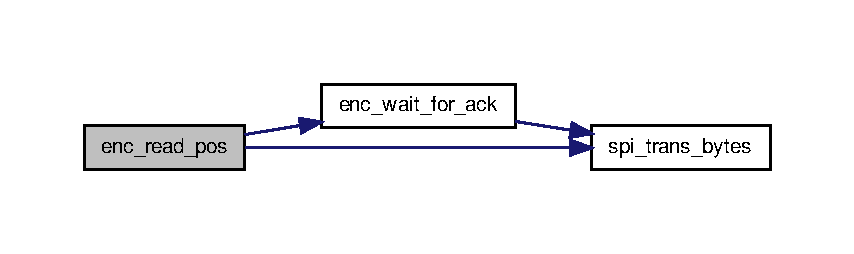
\includegraphics[width=350pt]{group__enc_ga813c09cc4d9af8b357fe440a9438e685_cgraph}
\end{center}
\end{figure}




Here is the caller graph for this function\-:
\nopagebreak
\begin{figure}[H]
\begin{center}
\leavevmode
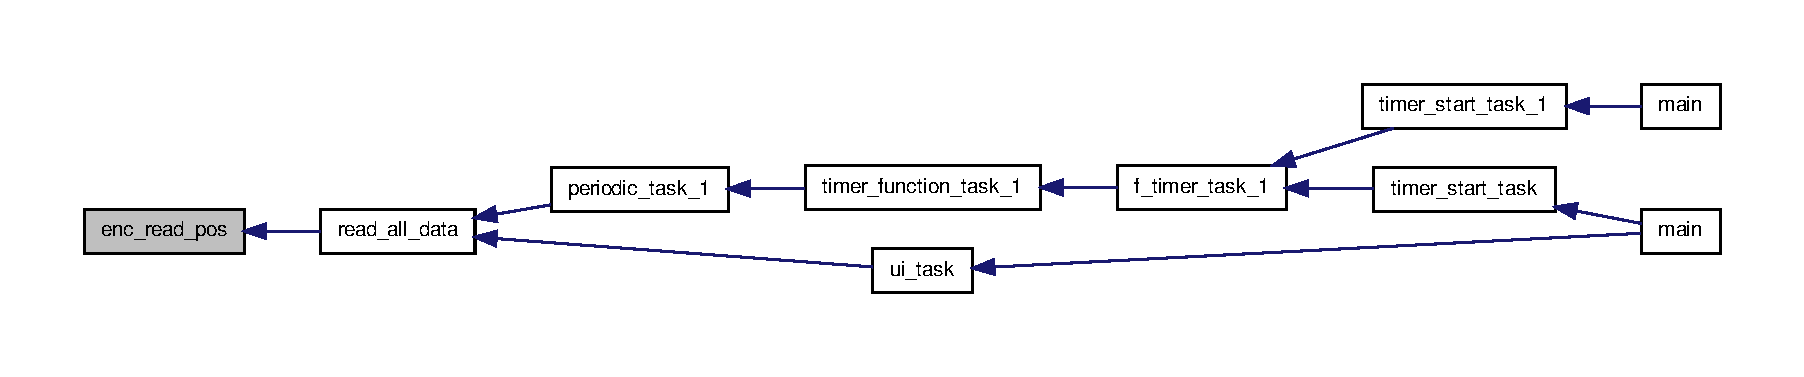
\includegraphics[width=350pt]{group__enc_ga813c09cc4d9af8b357fe440a9438e685_icgraph}
\end{center}
\end{figure}


\hypertarget{group__enc_gad82fb44f2e735628ec95e003e4a1f93c}{\index{Function of Encoder A\-M\-T203@{Function of Encoder A\-M\-T203}!enc\-\_\-wait\-\_\-for\-\_\-ack@{enc\-\_\-wait\-\_\-for\-\_\-ack}}
\index{enc\-\_\-wait\-\_\-for\-\_\-ack@{enc\-\_\-wait\-\_\-for\-\_\-ack}!Function of Encoder AMT203@{Function of Encoder A\-M\-T203}}
\subsubsection[{enc\-\_\-wait\-\_\-for\-\_\-ack}]{\setlength{\rightskip}{0pt plus 5cm}int enc\-\_\-wait\-\_\-for\-\_\-ack (
\begin{DoxyParamCaption}
\item[{int}]{spi\-\_\-dev, }
\item[{uint8\-\_\-t}]{ack, }
\item[{int}]{max\-\_\-errors}
\end{DoxyParamCaption}
)}}\label{group__enc_gad82fb44f2e735628ec95e003e4a1f93c}


send command and delay between reads 


\begin{DoxyParams}[1]{Parameters}
 & {\em spi\-\_\-dev} & Communication Dev \\
\hline
\mbox{\tt in}  & {\em data} & Data to write \\
\hline
\end{DoxyParams}
\begin{DoxyReturn}{Returns}
flag with S\-U\-C\-C\-E\-S\-S or F\-A\-I\-L\-U\-R\-E 
\end{DoxyReturn}


Definition at line 73 of file encoder\-\_\-functions.\-c.



References E\-N\-C\-O\-D\-E\-R\-\_\-\-N\-O\-\_\-\-O\-P, E\-N\-C\-O\-D\-E\-R\-\_\-\-W\-A\-I\-T\-\_\-\-R\-E\-S\-P, F\-A\-I\-L\-U\-R\-E, spi\-\_\-trans\-\_\-bytes(), and S\-U\-C\-C\-E\-S\-S.



Referenced by enc\-\_\-read\-\_\-pos(), and enc\-\_\-zero\-\_\-set().


\begin{DoxyCode}
\{
    \textcolor{keywordtype}{int} errors = 0;
    uint8\_t send = \hyperlink{encoder__functions_8h_ac10b0f18ed2164776ad6843aa7908592}{ENCODER\_NO\_OP};
    uint8\_t receive = 1;
        
  \textcolor{comment}{//nanosleep(10);}
        \textcolor{comment}{//spi\_trans\_bytes(spi\_dev,send,receive,1);}
    \textcolor{keywordflow}{while} (receive != ack) \{
        \hyperlink{spi__functions_8c_a3ae450d2b3ece27bb6036f811a7625a9}{spi\_trans\_bytes}(spi\_dev,&send,&receive,1);
        \textcolor{comment}{//printf("\(\backslash\)nReceive = 0x%x \(\backslash\)n",receive);}
        \textcolor{keywordflow}{if} (receive != \hyperlink{encoder__functions_8h_a77c3a97f7312d858d04ec3b4e1fb2176}{ENCODER\_WAIT\_RESP}) \{
            errors++;
            \textcolor{keywordflow}{if} (errors > max\_errors) \{ \textcolor{keywordflow}{return} \hyperlink{calibration_2calibration_8h_a6d58f9ac447476b4e084d7ca383f5183}{FAILURE}; \}
        \}
    \}


    \textcolor{keywordflow}{return} \hyperlink{calibration_2calibration_8h_aa90cac659d18e8ef6294c7ae337f6b58}{SUCCESS};
\}
\end{DoxyCode}


Here is the call graph for this function\-:
\nopagebreak
\begin{figure}[H]
\begin{center}
\leavevmode
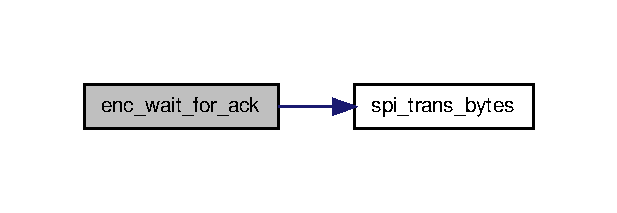
\includegraphics[width=296pt]{group__enc_gad82fb44f2e735628ec95e003e4a1f93c_cgraph}
\end{center}
\end{figure}




Here is the caller graph for this function\-:
\nopagebreak
\begin{figure}[H]
\begin{center}
\leavevmode
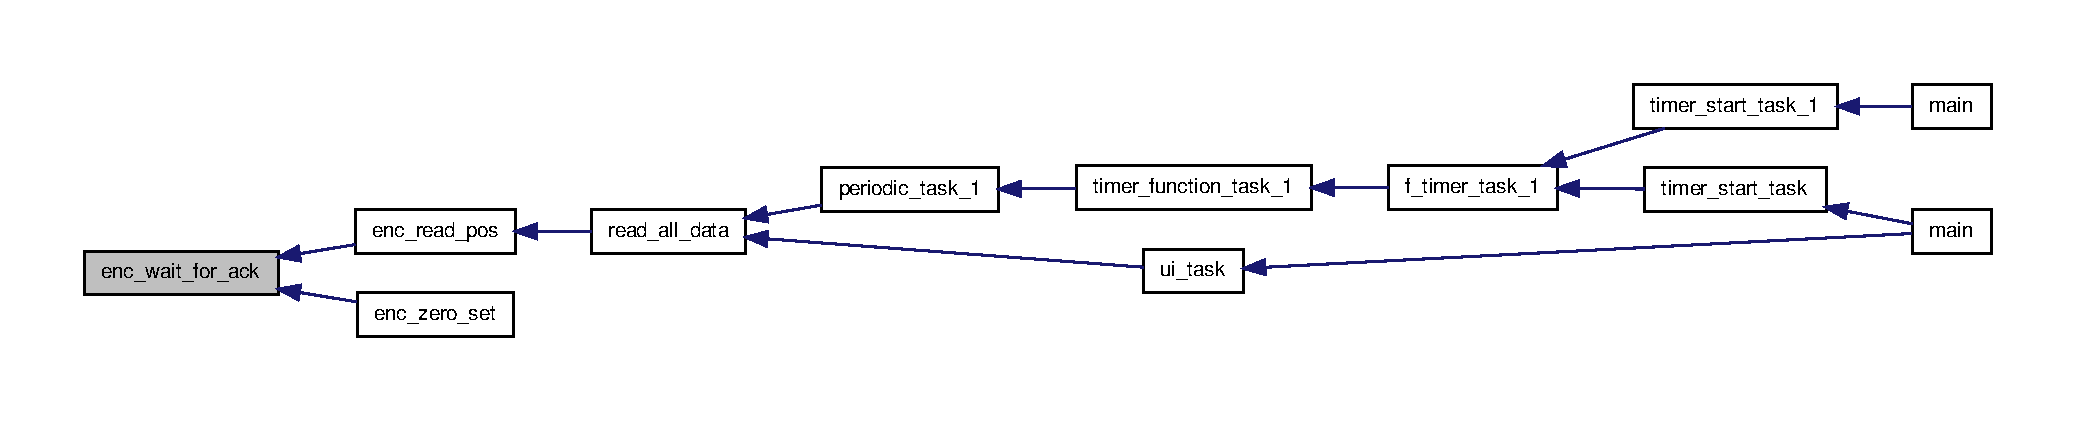
\includegraphics[width=350pt]{group__enc_gad82fb44f2e735628ec95e003e4a1f93c_icgraph}
\end{center}
\end{figure}


\hypertarget{group__enc_gaebbe7b9d3c2571f7481cefacbe36c498}{\index{Function of Encoder A\-M\-T203@{Function of Encoder A\-M\-T203}!enc\-\_\-zero\-\_\-set@{enc\-\_\-zero\-\_\-set}}
\index{enc\-\_\-zero\-\_\-set@{enc\-\_\-zero\-\_\-set}!Function of Encoder AMT203@{Function of Encoder A\-M\-T203}}
\subsubsection[{enc\-\_\-zero\-\_\-set}]{\setlength{\rightskip}{0pt plus 5cm}int enc\-\_\-zero\-\_\-set (
\begin{DoxyParamCaption}
\item[{int}]{spi\-\_\-dev}
\end{DoxyParamCaption}
)}}\label{group__enc_gaebbe7b9d3c2571f7481cefacbe36c498}


S\-E\-T Z\-E\-R\-O P\-O\-I\-N\-T. 


\begin{DoxyParams}[1]{Parameters}
 & {\em spi\-\_\-dev} & Communication Dev \\
\hline
\mbox{\tt in}  & {\em data} & Data to write\\
\hline
\end{DoxyParams}
\begin{DoxyReturn}{Returns}
flag with S\-U\-C\-C\-E\-S\-S or F\-A\-I\-L\-U\-R\-E 
\end{DoxyReturn}


Definition at line 19 of file encoder\-\_\-functions.\-c.



References enc\-\_\-wait\-\_\-for\-\_\-ack(), E\-N\-C\-O\-D\-E\-R\-\_\-\-E\-E\-P\-R\-O\-M\-\_\-\-W\-R, E\-N\-C\-O\-D\-E\-R\-\_\-\-S\-E\-T\-\_\-\-Z\-E\-R\-O\-\_\-\-P\-T, F\-A\-I\-L\-U\-R\-E, I\-N\-T\-\_\-\-M\-A\-X, spi\-\_\-trans\-\_\-bytes(), and S\-U\-C\-C\-E\-S\-S.


\begin{DoxyCode}
                             \{

    uint8\_t send = \hyperlink{encoder__functions_8h_aa2fec4e0eb5a7b3668158a57952b9dbe}{ENCODER\_SET\_ZERO\_PT};
    uint8\_t receive = 0;
    
    \textcolor{comment}{/* Send command */}
    \hyperlink{spi__functions_8c_a3ae450d2b3ece27bb6036f811a7625a9}{spi\_trans\_bytes}(spi\_dev,&send,&receive,1);
    \textcolor{keywordflow}{if} (\hyperlink{group__enc_gad82fb44f2e735628ec95e003e4a1f93c}{enc\_wait\_for\_ack}(spi\_dev, \hyperlink{encoder__functions_8h_ab815abd4b9b825c60dbb04aad0d0e846}{ENCODER\_EEPROM\_WR}
      , \hyperlink{encoder__functions_8h_a9ec306f36d50c7375e74f0d1c55a3a67}{INT\_MAX}) != \hyperlink{calibration_2calibration_8h_aa90cac659d18e8ef6294c7ae337f6b58}{SUCCESS})\{ 
        \textcolor{keywordflow}{return} \hyperlink{calibration_2calibration_8h_a6d58f9ac447476b4e084d7ca383f5183}{FAILURE};
    \}

    \textcolor{comment}{/* Note: }
\textcolor{comment}{     *   From datasheet, the encoder must be power-cycled after this command}
\textcolor{comment}{     *   for the new zero position to be used in the position calculation. */}

    \textcolor{keywordflow}{return} \hyperlink{calibration_2calibration_8h_aa90cac659d18e8ef6294c7ae337f6b58}{SUCCESS};
\}
\end{DoxyCode}


Here is the call graph for this function\-:
\nopagebreak
\begin{figure}[H]
\begin{center}
\leavevmode
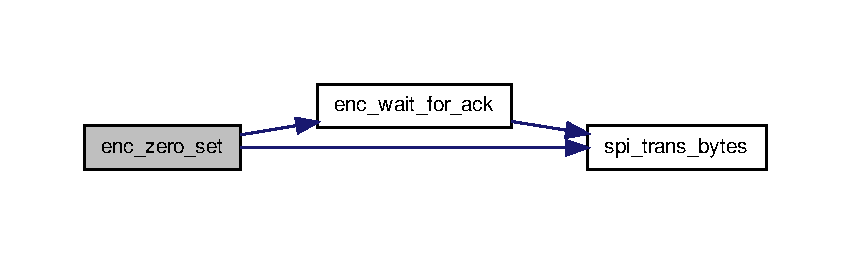
\includegraphics[width=350pt]{group__enc_gaebbe7b9d3c2571f7481cefacbe36c498_cgraph}
\end{center}
\end{figure}



\hypertarget{group__imu}{\section{I\-M\-U sensors}
\label{group__imu}\index{I\-M\-U sensors@{I\-M\-U sensors}}
}
Collaboration diagram for I\-M\-U sensors\-:
\nopagebreak
\begin{figure}[H]
\begin{center}
\leavevmode
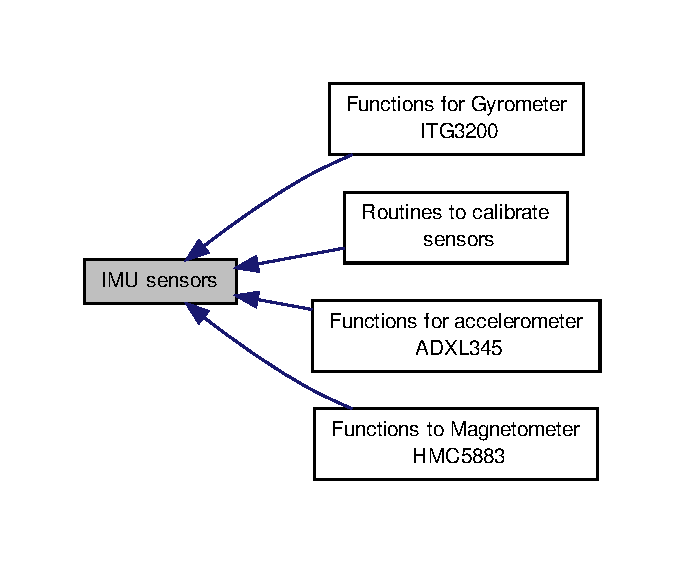
\includegraphics[width=328pt]{group__imu}
\end{center}
\end{figure}
\subsection*{Modules}
\begin{DoxyCompactItemize}
\item 
\hyperlink{group__calibrate}{Routines to calibrate sensors}
\item 
\hyperlink{group__acc}{Functions for accelerometer A\-D\-X\-L345}
\item 
\hyperlink{group__gyr}{Functions for Gyrometer I\-T\-G3200}
\item 
\hyperlink{group__mag}{Functions to Magnetometer H\-M\-C5883}
\end{DoxyCompactItemize}
\subsection*{Functions}
\begin{DoxyCompactItemize}
\item 
int \hyperlink{group__imu_gab5d0ae421cd4bb10b1b7a1eda167416b}{mag\-\_\-write\-\_\-reg} (int \hyperlink{CommunicationV0_2communication_8c_a7751bd45ac1064efb35adf1f19c25db8}{i2c\-\_\-dev}, uint8\-\_\-t reg, uint8\-\_\-t data)
\begin{DoxyCompactList}\small\item\em W\-R\-I\-T\-E T\-O R\-E\-G\-I\-S\-T\-E\-R. \end{DoxyCompactList}\end{DoxyCompactItemize}


\subsection{Detailed Description}


\subsection{Function Documentation}
\hypertarget{group__imu_gab5d0ae421cd4bb10b1b7a1eda167416b}{\index{I\-M\-U sensors@{I\-M\-U sensors}!mag\-\_\-write\-\_\-reg@{mag\-\_\-write\-\_\-reg}}
\index{mag\-\_\-write\-\_\-reg@{mag\-\_\-write\-\_\-reg}!IMU sensors@{I\-M\-U sensors}}
\subsubsection[{mag\-\_\-write\-\_\-reg}]{\setlength{\rightskip}{0pt plus 5cm}int mag\-\_\-write\-\_\-reg (
\begin{DoxyParamCaption}
\item[{int}]{i2c\-\_\-dev, }
\item[{uint8\-\_\-t}]{reg, }
\item[{uint8\-\_\-t}]{data}
\end{DoxyParamCaption}
)}}\label{group__imu_gab5d0ae421cd4bb10b1b7a1eda167416b}


W\-R\-I\-T\-E T\-O R\-E\-G\-I\-S\-T\-E\-R. 


\begin{DoxyParams}[1]{Parameters}
 & {\em i2c\-\_\-dev} & \\
\hline
 & {\em reg} & \\
\hline
\mbox{\tt in}  & {\em } & W\-R\-I\-T\-E T\-O R\-E\-G\-I\-S\-T\-E\-R.\\
\hline
\end{DoxyParams}
Implements the I2\-C communication between Gumstix Overo Fire and H\-M\-C5883 \begin{DoxyAuthor}{Author}
Caio Gustavo Mesquita Ângelo 
\end{DoxyAuthor}


Definition at line 10 of file mag\-\_\-functions.\-c.



Referenced by mag\-\_\-init().


\begin{DoxyCode}
11 \{
12   uint8\_t reg\_data[2];
13 
14   reg\_data[0] = reg;
15   reg\_data[1] = data;
16 
17   \textcolor{keywordflow}{if}( \hyperlink{communication_2imu__regs_8h_a0173afba6efc0e164495bf506a9758d2}{MAG\_MODE}<reg )
18   \{
19       \textcolor{comment}{//perror("Write unsucessful: Not a valid writable register");}
20       \textcolor{keywordflow}{return} -1;
21   \}
22         
23   \textcolor{keywordflow}{if} (write(\hyperlink{CommunicationV0_2communication_8c_a7751bd45ac1064efb35adf1f19c25db8}{i2c\_dev}, &reg\_data, 2) != 2) \{                
24           \textcolor{comment}{//perror("Write unsuccessful");}
25           \textcolor{keywordflow}{return} -1;
26   \}
27 
28   \textcolor{keywordflow}{return} 1;
29 \}
\end{DoxyCode}


Here is the caller graph for this function\-:
\nopagebreak
\begin{figure}[H]
\begin{center}
\leavevmode
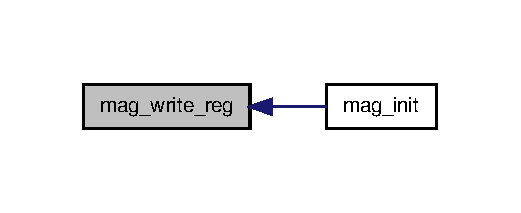
\includegraphics[width=250pt]{group__imu_gab5d0ae421cd4bb10b1b7a1eda167416b_icgraph}
\end{center}
\end{figure}



\hypertarget{group__acc}{\section{Functions for accelerometer A\-D\-X\-L345}
\label{group__acc}\index{Functions for accelerometer A\-D\-X\-L345@{Functions for accelerometer A\-D\-X\-L345}}
}
Collaboration diagram for Functions for accelerometer A\-D\-X\-L345\-:
\nopagebreak
\begin{figure}[H]
\begin{center}
\leavevmode
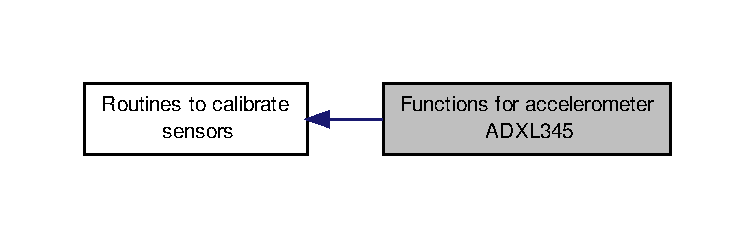
\includegraphics[width=350pt]{group__acc}
\end{center}
\end{figure}
\subsection*{Macros}
\begin{DoxyCompactItemize}
\item 
\#define \hyperlink{group__acc_ga355ea8f6ceed1e1d419a3ea2271bfca3}{A\-C\-C\-\_\-\-B\-I\-A\-S\-\_\-\-X}~19.\-2
\item 
\#define \hyperlink{group__acc_ga34180f1c97e84a814ef181f62bf4b68f}{A\-C\-C\-\_\-\-B\-I\-A\-S\-\_\-\-Y}~6.\-024
\item 
\#define \hyperlink{group__acc_ga794f762650b6f228ffb8d50d1323dbea}{A\-C\-C\-\_\-\-B\-I\-A\-S\-\_\-\-Z}~-\/18.\-97
\item 
\#define \hyperlink{group__acc_ga76e6967cb5a86ec34986b4583ac09831}{A\-C\-C\-\_\-\-F\-S\-\_\-\-X}~262.\-82
\item 
\#define \hyperlink{group__acc_ga13d3aaab3b5800b11351cbd1246c8918}{A\-C\-C\-\_\-\-F\-S\-\_\-\-Y}~262.\-15
\item 
\#define \hyperlink{group__acc_gaf1d3370cc0958289199c8c13470602d4}{A\-C\-C\-\_\-\-F\-S\-\_\-\-Z}~252.\-20
\end{DoxyCompactItemize}
\subsection*{Functions}
\begin{DoxyCompactItemize}
\item 
int \hyperlink{group__acc_ga534116416343122de29a5b6ade6876bd}{acc\-\_\-write\-\_\-reg} (int \hyperlink{CommunicationV0_2communication_8c_a7751bd45ac1064efb35adf1f19c25db8}{i2c\-\_\-dev}, uint8\-\_\-t reg, uint8\-\_\-t data)
\begin{DoxyCompactList}\small\item\em W\-R\-I\-T\-E T\-O R\-E\-G\-I\-S\-T\-E\-R. \end{DoxyCompactList}\item 
uint8\-\_\-t $\ast$ \hyperlink{group__acc_ga2a91c44eebbe44f4d3b8c508633512f9}{acc\-\_\-read\-\_\-reg} (int \hyperlink{CommunicationV0_2communication_8c_a7751bd45ac1064efb35adf1f19c25db8}{i2c\-\_\-dev}, uint8\-\_\-t reg, uint8\-\_\-t count)
\begin{DoxyCompactList}\small\item\em R\-E\-A\-D C\-O\-U\-N\-T 8-\/\-B\-I\-T R\-E\-G\-I\-S\-T\-E\-R I\-N S\-E\-Q\-U\-E\-N\-C\-E \end{DoxyCompactList}\item 
int \hyperlink{group__acc_gae8f9cc6e0d15e61039d846305f86f073}{acc\-\_\-init} (int \hyperlink{CommunicationV0_2communication_8c_a7751bd45ac1064efb35adf1f19c25db8}{i2c\-\_\-dev}, uint8\-\_\-t full\-\_\-res, uint16\-\_\-t rate, uint8\-\_\-t range)
\begin{DoxyCompactList}\small\item\em I\-N\-I\-T\-I\-A\-L\-I\-Z\-E A\-C\-C\-E\-L\-E\-R\-O\-M\-E\-T\-E\-R. \end{DoxyCompactList}\item 
int \hyperlink{group__acc_ga013bb5ed8a763883fc440549d2b1a6ce}{acc\-\_\-read\-\_\-all\-\_\-data} (int \hyperlink{CommunicationV0_2communication_8c_a7751bd45ac1064efb35adf1f19c25db8}{i2c\-\_\-dev}, short int $\ast$data)
\begin{DoxyCompactList}\small\item\em R\-E\-A\-D A\-L\-L D\-A\-T\-A A\-T O\-N\-C\-E (X, Y and Z) \end{DoxyCompactList}\item 
short int \hyperlink{group__acc_ga041d6953f2bfc8c5efa4d5bbac812305}{acc\-\_\-read\-\_\-data} (int \hyperlink{CommunicationV0_2communication_8c_a7751bd45ac1064efb35adf1f19c25db8}{i2c\-\_\-dev}, int axis)
\begin{DoxyCompactList}\small\item\em R\-E\-A\-D D\-A\-T\-A (X, Y or Z) \end{DoxyCompactList}\item 
int \hyperlink{group__acc_ga8509cccabb08e7267677f66f25718731}{acc\-\_\-read\-\_\-all\-\_\-reg} (int \hyperlink{CommunicationV0_2communication_8c_a7751bd45ac1064efb35adf1f19c25db8}{i2c\-\_\-dev})
\begin{DoxyCompactList}\small\item\em Read all accelerometer data and print in stdio. \end{DoxyCompactList}\end{DoxyCompactItemize}


\subsection{Detailed Description}


\subsection{Macro Definition Documentation}
\hypertarget{group__acc_ga355ea8f6ceed1e1d419a3ea2271bfca3}{\index{Functions for accelerometer A\-D\-X\-L345@{Functions for accelerometer A\-D\-X\-L345}!A\-C\-C\-\_\-\-B\-I\-A\-S\-\_\-\-X@{A\-C\-C\-\_\-\-B\-I\-A\-S\-\_\-\-X}}
\index{A\-C\-C\-\_\-\-B\-I\-A\-S\-\_\-\-X@{A\-C\-C\-\_\-\-B\-I\-A\-S\-\_\-\-X}!Functions for accelerometer ADXL345@{Functions for accelerometer A\-D\-X\-L345}}
\subsubsection[{A\-C\-C\-\_\-\-B\-I\-A\-S\-\_\-\-X}]{\setlength{\rightskip}{0pt plus 5cm}\#define A\-C\-C\-\_\-\-B\-I\-A\-S\-\_\-\-X~19.\-2}}\label{group__acc_ga355ea8f6ceed1e1d419a3ea2271bfca3}


Definition at line 19 of file calibration.\-h.



Referenced by calibrate\-\_\-imu().

\hypertarget{group__acc_ga34180f1c97e84a814ef181f62bf4b68f}{\index{Functions for accelerometer A\-D\-X\-L345@{Functions for accelerometer A\-D\-X\-L345}!A\-C\-C\-\_\-\-B\-I\-A\-S\-\_\-\-Y@{A\-C\-C\-\_\-\-B\-I\-A\-S\-\_\-\-Y}}
\index{A\-C\-C\-\_\-\-B\-I\-A\-S\-\_\-\-Y@{A\-C\-C\-\_\-\-B\-I\-A\-S\-\_\-\-Y}!Functions for accelerometer ADXL345@{Functions for accelerometer A\-D\-X\-L345}}
\subsubsection[{A\-C\-C\-\_\-\-B\-I\-A\-S\-\_\-\-Y}]{\setlength{\rightskip}{0pt plus 5cm}\#define A\-C\-C\-\_\-\-B\-I\-A\-S\-\_\-\-Y~6.\-024}}\label{group__acc_ga34180f1c97e84a814ef181f62bf4b68f}


Definition at line 20 of file calibration.\-h.



Referenced by calibrate\-\_\-imu().

\hypertarget{group__acc_ga794f762650b6f228ffb8d50d1323dbea}{\index{Functions for accelerometer A\-D\-X\-L345@{Functions for accelerometer A\-D\-X\-L345}!A\-C\-C\-\_\-\-B\-I\-A\-S\-\_\-\-Z@{A\-C\-C\-\_\-\-B\-I\-A\-S\-\_\-\-Z}}
\index{A\-C\-C\-\_\-\-B\-I\-A\-S\-\_\-\-Z@{A\-C\-C\-\_\-\-B\-I\-A\-S\-\_\-\-Z}!Functions for accelerometer ADXL345@{Functions for accelerometer A\-D\-X\-L345}}
\subsubsection[{A\-C\-C\-\_\-\-B\-I\-A\-S\-\_\-\-Z}]{\setlength{\rightskip}{0pt plus 5cm}\#define A\-C\-C\-\_\-\-B\-I\-A\-S\-\_\-\-Z~-\/18.\-97}}\label{group__acc_ga794f762650b6f228ffb8d50d1323dbea}


Definition at line 21 of file calibration.\-h.



Referenced by calibrate\-\_\-imu().

\hypertarget{group__acc_ga76e6967cb5a86ec34986b4583ac09831}{\index{Functions for accelerometer A\-D\-X\-L345@{Functions for accelerometer A\-D\-X\-L345}!A\-C\-C\-\_\-\-F\-S\-\_\-\-X@{A\-C\-C\-\_\-\-F\-S\-\_\-\-X}}
\index{A\-C\-C\-\_\-\-F\-S\-\_\-\-X@{A\-C\-C\-\_\-\-F\-S\-\_\-\-X}!Functions for accelerometer ADXL345@{Functions for accelerometer A\-D\-X\-L345}}
\subsubsection[{A\-C\-C\-\_\-\-F\-S\-\_\-\-X}]{\setlength{\rightskip}{0pt plus 5cm}\#define A\-C\-C\-\_\-\-F\-S\-\_\-\-X~262.\-82}}\label{group__acc_ga76e6967cb5a86ec34986b4583ac09831}


Definition at line 22 of file calibration.\-h.



Referenced by calibrate\-\_\-imu().

\hypertarget{group__acc_ga13d3aaab3b5800b11351cbd1246c8918}{\index{Functions for accelerometer A\-D\-X\-L345@{Functions for accelerometer A\-D\-X\-L345}!A\-C\-C\-\_\-\-F\-S\-\_\-\-Y@{A\-C\-C\-\_\-\-F\-S\-\_\-\-Y}}
\index{A\-C\-C\-\_\-\-F\-S\-\_\-\-Y@{A\-C\-C\-\_\-\-F\-S\-\_\-\-Y}!Functions for accelerometer ADXL345@{Functions for accelerometer A\-D\-X\-L345}}
\subsubsection[{A\-C\-C\-\_\-\-F\-S\-\_\-\-Y}]{\setlength{\rightskip}{0pt plus 5cm}\#define A\-C\-C\-\_\-\-F\-S\-\_\-\-Y~262.\-15}}\label{group__acc_ga13d3aaab3b5800b11351cbd1246c8918}


Definition at line 23 of file calibration.\-h.



Referenced by calibrate\-\_\-imu().

\hypertarget{group__acc_gaf1d3370cc0958289199c8c13470602d4}{\index{Functions for accelerometer A\-D\-X\-L345@{Functions for accelerometer A\-D\-X\-L345}!A\-C\-C\-\_\-\-F\-S\-\_\-\-Z@{A\-C\-C\-\_\-\-F\-S\-\_\-\-Z}}
\index{A\-C\-C\-\_\-\-F\-S\-\_\-\-Z@{A\-C\-C\-\_\-\-F\-S\-\_\-\-Z}!Functions for accelerometer ADXL345@{Functions for accelerometer A\-D\-X\-L345}}
\subsubsection[{A\-C\-C\-\_\-\-F\-S\-\_\-\-Z}]{\setlength{\rightskip}{0pt plus 5cm}\#define A\-C\-C\-\_\-\-F\-S\-\_\-\-Z~252.\-20}}\label{group__acc_gaf1d3370cc0958289199c8c13470602d4}


Definition at line 24 of file calibration.\-h.



Referenced by calibrate\-\_\-imu().



\subsection{Function Documentation}
\hypertarget{group__acc_gae8f9cc6e0d15e61039d846305f86f073}{\index{Functions for accelerometer A\-D\-X\-L345@{Functions for accelerometer A\-D\-X\-L345}!acc\-\_\-init@{acc\-\_\-init}}
\index{acc\-\_\-init@{acc\-\_\-init}!Functions for accelerometer ADXL345@{Functions for accelerometer A\-D\-X\-L345}}
\subsubsection[{acc\-\_\-init}]{\setlength{\rightskip}{0pt plus 5cm}int acc\-\_\-init (
\begin{DoxyParamCaption}
\item[{int}]{i2c\-\_\-dev, }
\item[{uint8\-\_\-t}]{full\-\_\-res, }
\item[{uint16\-\_\-t}]{rate, }
\item[{uint8\-\_\-t}]{range}
\end{DoxyParamCaption}
)}}\label{group__acc_gae8f9cc6e0d15e61039d846305f86f073}


I\-N\-I\-T\-I\-A\-L\-I\-Z\-E A\-C\-C\-E\-L\-E\-R\-O\-M\-E\-T\-E\-R. 


\begin{DoxyParams}{Parameters}
{\em i2c\-\_\-dev} & Communication Port \\
\hline
{\em full\-\_\-res} & Set resolution to 10 bits if value equal 0 else set to Full resolution \\
\hline
{\em rate} & Set data output rate (Hz), possible values\-: (3200,1600,800,400,200,100,50,25, 12\-: 12.\-5\-Hz, 6\-: 6.\-25\-Hz) \\
\hline
{\em range} & Set range of read, possible values\-: (2\-: +-\/ 2g 4\-: +-\/ 4g 8\-: +-\/ 8g anyother\-: 16g) \\
\hline
\end{DoxyParams}
\begin{DoxyReturn}{Returns}
flag with S\-U\-C\-C\-E\-S\-S or F\-A\-I\-L\-U\-R\-E
\end{DoxyReturn}
I\-N\-I\-T\-I\-A\-L\-I\-Z\-E A\-C\-C\-E\-L\-E\-R\-O\-M\-E\-T\-E\-R.

Implements the I2\-C communication between Gumstix Overo Fire and A\-D\-X\-L345 \begin{DoxyAuthor}{Author}
Caio Gustavo Mesquita Ângelo 
\end{DoxyAuthor}


Definition at line 11 of file acc\-\_\-functions.\-c.


\begin{DoxyCode}
\{ 
  uint8\_t data=0;

  \textcolor{keywordflow}{switch}(range)\{
    \textcolor{keywordflow}{case} 2:
      data=0x08;;
      \textcolor{keywordflow}{break};
    \textcolor{keywordflow}{case} 4:
      data=0x09;
      \textcolor{keywordflow}{break};
    \textcolor{keywordflow}{case} 8:
      data=0x0A;
      \textcolor{keywordflow}{break};
    \textcolor{keywordflow}{default}:
      data=0x0B;
      \textcolor{keywordflow}{break};
  \}
  
  \textcolor{keywordflow}{if}(full\_res==0)
    data=data&(0xF7);
  
  \textcolor{keywordflow}{if}((\hyperlink{group__acc_ga534116416343122de29a5b6ade6876bd}{acc\_write\_reg}(\hyperlink{CommunicationV0_2communication_8c_a7751bd45ac1064efb35adf1f19c25db8}{i2c\_dev}, \hyperlink{communication_2imu__regs_8h_ab4eb7fc69b2a37ee750d3400fc2c53a1}{ACC\_DATA\_FORMAT}
      , data))<0)\{
    perror(\textcolor{stringliteral}{"Data Format unsuccesful"});
    \textcolor{keywordflow}{return} \hyperlink{calibration_2calibration_8h_a6d58f9ac447476b4e084d7ca383f5183}{FAILURE};
  \}
  
  data=\hyperlink{communication_2imu__regs_8h_a9a841ba3e094b01ea439584e12b25894}{ACC\_POWER\_CTL\_MEAS\_MODE};
  \textcolor{keywordflow}{if}((\hyperlink{group__acc_ga534116416343122de29a5b6ade6876bd}{acc\_write\_reg}(\hyperlink{CommunicationV0_2communication_8c_a7751bd45ac1064efb35adf1f19c25db8}{i2c\_dev}, \hyperlink{communication_2imu__regs_8h_ad857d62b61f349216faeda06eff5f9c6}{ACC\_POWER\_CTL}, 
      data))<0)\{
    perror(\textcolor{stringliteral}{"Power Control unsuccesful"});
    \textcolor{keywordflow}{return} \hyperlink{calibration_2calibration_8h_a6d58f9ac447476b4e084d7ca383f5183}{FAILURE};
  \}
  
  \textcolor{keywordflow}{switch}(rate)\{
    \textcolor{keywordflow}{case} 100:
      data=0x0A;
      \textcolor{keywordflow}{break};
    \textcolor{keywordflow}{case} 3200:
      data=0x0F;;
      \textcolor{keywordflow}{break};
    \textcolor{keywordflow}{case} 1600:
      data=0x0E;
      \textcolor{keywordflow}{break};
    \textcolor{keywordflow}{case} 800:
      data=0x0D;
      \textcolor{keywordflow}{break};
    \textcolor{keywordflow}{case} 400:
      data=0x0C;
      \textcolor{keywordflow}{break};
    \textcolor{keywordflow}{case} 200:
      data=0x0B;
      \textcolor{keywordflow}{break};
    \textcolor{keywordflow}{case} 50:
      data=0x09;
      \textcolor{keywordflow}{break}; 
    \textcolor{keywordflow}{case} 25:
      data=0x08;
      \textcolor{keywordflow}{break};
    \textcolor{keywordflow}{case} 12:
      data=0x07;
      \textcolor{keywordflow}{break};
    \textcolor{keywordflow}{case} 6:
      data=0x06;
      \textcolor{keywordflow}{break};
    \textcolor{keywordflow}{default}:
      perror(\textcolor{stringliteral}{"Wrong rate value"});
      \textcolor{keywordflow}{return} \hyperlink{calibration_2calibration_8h_a6d58f9ac447476b4e084d7ca383f5183}{FAILURE};
  \}
  \textcolor{keywordflow}{if}((\hyperlink{group__acc_ga534116416343122de29a5b6ade6876bd}{acc\_write\_reg}(\hyperlink{CommunicationV0_2communication_8c_a7751bd45ac1064efb35adf1f19c25db8}{i2c\_dev}, \hyperlink{communication_2imu__regs_8h_afbbb5a3aa097a32f98c47158141a882f}{ACC\_BW\_RATE}, data))
      <0)\{
    perror(\textcolor{stringliteral}{"Write in BW\_RATE unsuccesful"});
    \textcolor{keywordflow}{return} \hyperlink{calibration_2calibration_8h_a6d58f9ac447476b4e084d7ca383f5183}{FAILURE};
  \}
  
  \textcolor{keywordflow}{return} \hyperlink{calibration_2calibration_8h_aa90cac659d18e8ef6294c7ae337f6b58}{SUCCESS};
\}
\end{DoxyCode}
\hypertarget{group__acc_ga013bb5ed8a763883fc440549d2b1a6ce}{\index{Functions for accelerometer A\-D\-X\-L345@{Functions for accelerometer A\-D\-X\-L345}!acc\-\_\-read\-\_\-all\-\_\-data@{acc\-\_\-read\-\_\-all\-\_\-data}}
\index{acc\-\_\-read\-\_\-all\-\_\-data@{acc\-\_\-read\-\_\-all\-\_\-data}!Functions for accelerometer ADXL345@{Functions for accelerometer A\-D\-X\-L345}}
\subsubsection[{acc\-\_\-read\-\_\-all\-\_\-data}]{\setlength{\rightskip}{0pt plus 5cm}int acc\-\_\-read\-\_\-all\-\_\-data (
\begin{DoxyParamCaption}
\item[{int}]{i2c\-\_\-dev, }
\item[{short int $\ast$}]{data}
\end{DoxyParamCaption}
)}}\label{group__acc_ga013bb5ed8a763883fc440549d2b1a6ce}


R\-E\-A\-D A\-L\-L D\-A\-T\-A A\-T O\-N\-C\-E (X, Y and Z) 


\begin{DoxyParams}[1]{Parameters}
 & {\em i2c\-\_\-dev} & Communication Port \\
\hline
\mbox{\tt out}  & {\em data} & Data's vector\\
\hline
\end{DoxyParams}
\begin{DoxyReturn}{Returns}
flag with S\-U\-C\-C\-E\-S\-S or F\-A\-I\-L\-U\-R\-E 
\end{DoxyReturn}


Definition at line 159 of file acc\-\_\-functions.\-c.


\begin{DoxyCode}
\{
  \textcolor{keywordtype}{int} i;
  uint8\_t *data8;
  \textcolor{keyword}{union }result
  \{
    \textcolor{keywordtype}{unsigned} \textcolor{keywordtype}{short} \textcolor{keywordtype}{int} usgnd[3];
    \textcolor{keywordtype}{short} \textcolor{keywordtype}{int} sgnd[3];
  \} result;
  \textcolor{comment}{//result=(union result*)malloc(3*sizeof(union result));}
  \textcolor{keywordflow}{if}( (data8=\hyperlink{group__acc_ga2a91c44eebbe44f4d3b8c508633512f9}{acc\_read\_reg}(\hyperlink{CommunicationV0_2communication_8c_a7751bd45ac1064efb35adf1f19c25db8}{i2c\_dev},\hyperlink{communication_2imu__regs_8h_afae448fbad872220013e5c3abf0f3d9f}{ACC\_DATAX0},6))==
      NULL )
  \{
    \textcolor{comment}{//perror("Read accelerometer register failed");}
    \textcolor{keywordflow}{return} \hyperlink{calibration_2calibration_8h_a6d58f9ac447476b4e084d7ca383f5183}{FAILURE};
  \}
  \textcolor{comment}{//result.usgnd=(unsigned int*)malloc(3*sizeof(unsigned int));}
  \textcolor{keywordflow}{for}(i=0; i<3; i++)
  \{
    result.usgnd[i]=0;
    result.usgnd[i]=result.usgnd[i]|((\textcolor{keywordtype}{unsigned} \textcolor{keywordtype}{short} int)data8[i*2])|(((\textcolor{keywordtype}{
      unsigned} \textcolor{keywordtype}{short} int)data8[i*2+1])<<8);
    data[i]=result.sgnd[i];
  \}
  \textcolor{keywordflow}{return} \hyperlink{calibration_2calibration_8h_aa90cac659d18e8ef6294c7ae337f6b58}{SUCCESS};  
\}
\end{DoxyCode}
\hypertarget{group__acc_ga8509cccabb08e7267677f66f25718731}{\index{Functions for accelerometer A\-D\-X\-L345@{Functions for accelerometer A\-D\-X\-L345}!acc\-\_\-read\-\_\-all\-\_\-reg@{acc\-\_\-read\-\_\-all\-\_\-reg}}
\index{acc\-\_\-read\-\_\-all\-\_\-reg@{acc\-\_\-read\-\_\-all\-\_\-reg}!Functions for accelerometer ADXL345@{Functions for accelerometer A\-D\-X\-L345}}
\subsubsection[{acc\-\_\-read\-\_\-all\-\_\-reg}]{\setlength{\rightskip}{0pt plus 5cm}int acc\-\_\-read\-\_\-all\-\_\-reg (
\begin{DoxyParamCaption}
\item[{int}]{i2c\-\_\-dev}
\end{DoxyParamCaption}
)}}\label{group__acc_ga8509cccabb08e7267677f66f25718731}


Read all accelerometer data and print in stdio. 


\begin{DoxyParams}{Parameters}
{\em i2c\-\_\-dev} & Communication Port \\
\hline
\end{DoxyParams}


Definition at line 196 of file acc\-\_\-functions.\-c.


\begin{DoxyCode}
\{
  uint8\_t *hvalue0, *hvalue1, *hvalue;
  \textcolor{keywordtype}{int} i;
  
  hvalue0=\hyperlink{group__acc_ga2a91c44eebbe44f4d3b8c508633512f9}{acc\_read\_reg}(\hyperlink{CommunicationV0_2communication_8c_a7751bd45ac1064efb35adf1f19c25db8}{i2c\_dev},\hyperlink{communication_2imu__regs_8h_a007fa8d8ef9d89127ae5da32a2f42283}{ACC\_DEVID},1);
  printf(\textcolor{stringliteral}{"\(\backslash\)nhey"});
  printf(\textcolor{stringliteral}{"\(\backslash\)nhey3"});
  printf(\textcolor{stringliteral}{"\(\backslash\)nhey2"});
  printf(\textcolor{stringliteral}{"\(\backslash\)nhey3"});
  hvalue1=\hyperlink{group__acc_ga2a91c44eebbe44f4d3b8c508633512f9}{acc\_read\_reg}(\hyperlink{CommunicationV0_2communication_8c_a7751bd45ac1064efb35adf1f19c25db8}{i2c\_dev},\hyperlink{communication_2imu__regs_8h_afa5af181c4af31e22baa9bd20ff322ef}{ACC\_THRESH\_TAP},
       29);
  printf(\textcolor{stringliteral}{"\(\backslash\)nhey3"});
  \textcolor{comment}{//hvalue--;}
  hvalue=(uint8\_t*)malloc(30*\textcolor{keyword}{sizeof}(uint8\_t));
  hvalue[0]=hvalue0[0];
  \textcolor{keywordflow}{for}( i=0; i<29; i++)
    hvalue[i+1]=hvalue1[i];
  printf(\textcolor{stringliteral}{"\(\backslash\)nhey4"});
  printf(\textcolor{stringliteral}{"\(\backslash\)nACC\_DEVID = 0x%02X = %s"}, hvalue0[0],\hyperlink{communication_2acc__functions_8c_a1a6b2f719b4fef8f97d6d1b8f495148e}{conv\_byte\_hex\_bin}
      (hvalue0));
  printf(\textcolor{stringliteral}{"\(\backslash\)nACC\_THRESH\_TAP = 0x%02X = %s"}, hvalue1[0],\hyperlink{communication_2acc__functions_8c_a1a6b2f719b4fef8f97d6d1b8f495148e}{conv\_byte\_hex\_bin}
      (hvalue+1));
  printf(\textcolor{stringliteral}{"\(\backslash\)nACC\_OFSX = 0x%02X = %s"}, hvalue[2],\hyperlink{communication_2acc__functions_8c_a1a6b2f719b4fef8f97d6d1b8f495148e}{conv\_byte\_hex\_bin}
      (hvalue+2));
  printf(\textcolor{stringliteral}{"\(\backslash\)nACC\_OFSY = 0x%02X = %s"}, hvalue[3],\hyperlink{communication_2acc__functions_8c_a1a6b2f719b4fef8f97d6d1b8f495148e}{conv\_byte\_hex\_bin}
      (hvalue+3));
  printf(\textcolor{stringliteral}{"\(\backslash\)nACC\_OFSZ = 0x%02X = %s"}, hvalue[4],\hyperlink{communication_2acc__functions_8c_a1a6b2f719b4fef8f97d6d1b8f495148e}{conv\_byte\_hex\_bin}
      (hvalue+4));
  printf(\textcolor{stringliteral}{"\(\backslash\)nACC\_DUR = 0x%02X = %s"}, hvalue[5],\hyperlink{communication_2acc__functions_8c_a1a6b2f719b4fef8f97d6d1b8f495148e}{conv\_byte\_hex\_bin}
      (hvalue+5));
  printf(\textcolor{stringliteral}{"\(\backslash\)nACC\_LATENT = 0x%02X = %s"}, hvalue[6],\hyperlink{communication_2acc__functions_8c_a1a6b2f719b4fef8f97d6d1b8f495148e}{conv\_byte\_hex\_bin}
      (hvalue+6));
  printf(\textcolor{stringliteral}{"\(\backslash\)nACC\_WINDOW = 0x%02X = %s"}, hvalue[7],\hyperlink{communication_2acc__functions_8c_a1a6b2f719b4fef8f97d6d1b8f495148e}{conv\_byte\_hex\_bin}
      (hvalue+7));
  printf(\textcolor{stringliteral}{"\(\backslash\)nACC\_THRESH\_ACT = 0x%02X = %s"}, hvalue[8],\hyperlink{communication_2acc__functions_8c_a1a6b2f719b4fef8f97d6d1b8f495148e}{conv\_byte\_hex\_bin}
      (hvalue+8));
  printf(\textcolor{stringliteral}{"\(\backslash\)nACC\_THRESH\_INACT = 0x%02X = %s"}, hvalue[9],\hyperlink{communication_2acc__functions_8c_a1a6b2f719b4fef8f97d6d1b8f495148e}{conv\_byte\_hex\_bin}
      (hvalue+9));
  printf(\textcolor{stringliteral}{"\(\backslash\)nACC\_TIME\_INACT = 0x%02X = %s"}, hvalue[10],\hyperlink{communication_2acc__functions_8c_a1a6b2f719b4fef8f97d6d1b8f495148e}{conv\_byte\_hex\_bin}
      (hvalue+10));
  printf(\textcolor{stringliteral}{"\(\backslash\)nACC\_ACT\_INACT\_CTL = 0x%02X = %s"}, hvalue[11],\hyperlink{communication_2acc__functions_8c_a1a6b2f719b4fef8f97d6d1b8f495148e}{conv\_byte\_hex\_bin}
      (hvalue+11));
  printf(\textcolor{stringliteral}{"\(\backslash\)nACC\_THRESH\_FF = 0x%02X = %s"}, hvalue[12],\hyperlink{communication_2acc__functions_8c_a1a6b2f719b4fef8f97d6d1b8f495148e}{conv\_byte\_hex\_bin}
      (hvalue+12));
  printf(\textcolor{stringliteral}{"\(\backslash\)nACC\_TIME\_FF = 0x%02X = %s"}, hvalue[13],\hyperlink{communication_2acc__functions_8c_a1a6b2f719b4fef8f97d6d1b8f495148e}{conv\_byte\_hex\_bin}
      (hvalue+13));
  printf(\textcolor{stringliteral}{"\(\backslash\)nACC\_TAP\_AXES = 0x%02X = %s"}, hvalue[14],\hyperlink{communication_2acc__functions_8c_a1a6b2f719b4fef8f97d6d1b8f495148e}{conv\_byte\_hex\_bin}
      (hvalue+14));
  printf(\textcolor{stringliteral}{"\(\backslash\)nACC\_ACT\_TAP\_STATUS = 0x%02X = %s"}, hvalue[15],\hyperlink{communication_2acc__functions_8c_a1a6b2f719b4fef8f97d6d1b8f495148e}{conv\_byte\_hex\_bin}
      (hvalue+15));
  printf(\textcolor{stringliteral}{"\(\backslash\)nACC\_BW\_RATE = 0x%02X = %s"}, hvalue[16],\hyperlink{communication_2acc__functions_8c_a1a6b2f719b4fef8f97d6d1b8f495148e}{conv\_byte\_hex\_bin}
      (hvalue+16));
  printf(\textcolor{stringliteral}{"\(\backslash\)nACC\_POWER\_CTL = 0x%02X = %s"}, hvalue[17],\hyperlink{communication_2acc__functions_8c_a1a6b2f719b4fef8f97d6d1b8f495148e}{conv\_byte\_hex\_bin}
      (hvalue+17));
  printf(\textcolor{stringliteral}{"\(\backslash\)nACC\_INT\_ENABLE = 0x%02X = %s"}, hvalue[18],\hyperlink{communication_2acc__functions_8c_a1a6b2f719b4fef8f97d6d1b8f495148e}{conv\_byte\_hex\_bin}
      (hvalue+18));
  printf(\textcolor{stringliteral}{"\(\backslash\)nACC\_INT\_MAP = 0x%02X = %s"}, hvalue[19],\hyperlink{communication_2acc__functions_8c_a1a6b2f719b4fef8f97d6d1b8f495148e}{conv\_byte\_hex\_bin}
      (hvalue+19));
  printf(\textcolor{stringliteral}{"\(\backslash\)nACC\_INT\_SOURCE = 0x%02X = %s"}, hvalue[20],\hyperlink{communication_2acc__functions_8c_a1a6b2f719b4fef8f97d6d1b8f495148e}{conv\_byte\_hex\_bin}
      (hvalue+20));
  printf(\textcolor{stringliteral}{"\(\backslash\)nACC\_DATA\_FORMAT = 0x%02X = %s"}, hvalue1[20],\hyperlink{communication_2acc__functions_8c_a1a6b2f719b4fef8f97d6d1b8f495148e}{conv\_byte\_hex\_bin}
      (hvalue1+21));
  printf(\textcolor{stringliteral}{"\(\backslash\)nACC\_DATAX0 = 0x%02X = %s"}, hvalue1[21],\hyperlink{communication_2acc__functions_8c_a1a6b2f719b4fef8f97d6d1b8f495148e}{conv\_byte\_hex\_bin}
      (hvalue1+22));
  printf(\textcolor{stringliteral}{"\(\backslash\)nACC\_DATAX1 = 0x%02X = %s"}, hvalue1[22],\hyperlink{communication_2acc__functions_8c_a1a6b2f719b4fef8f97d6d1b8f495148e}{conv\_byte\_hex\_bin}
      (hvalue1+23));
  printf(\textcolor{stringliteral}{"\(\backslash\)nACC\_DATAY0 = 0x%02X = %s"}, hvalue1[23],\hyperlink{communication_2acc__functions_8c_a1a6b2f719b4fef8f97d6d1b8f495148e}{conv\_byte\_hex\_bin}
      (hvalue1+24));
  printf(\textcolor{stringliteral}{"\(\backslash\)nACC\_DATAY1 = 0x%02X = %s"}, hvalue1[24],\hyperlink{communication_2acc__functions_8c_a1a6b2f719b4fef8f97d6d1b8f495148e}{conv\_byte\_hex\_bin}
      (hvalue1+25));
  printf(\textcolor{stringliteral}{"\(\backslash\)nACC\_DATAZ0 = 0x%02X = %s"}, hvalue1[25],\hyperlink{communication_2acc__functions_8c_a1a6b2f719b4fef8f97d6d1b8f495148e}{conv\_byte\_hex\_bin}
      (hvalue1+26));
  printf(\textcolor{stringliteral}{"\(\backslash\)nACC\_DATAZ1 = 0x%02X = %s"}, hvalue1[26],\hyperlink{communication_2acc__functions_8c_a1a6b2f719b4fef8f97d6d1b8f495148e}{conv\_byte\_hex\_bin}
      (hvalue1+27));
  printf(\textcolor{stringliteral}{"\(\backslash\)nACC\_FIFO\_CTL = 0x%02X = %s"}, hvalue[28],\hyperlink{communication_2acc__functions_8c_a1a6b2f719b4fef8f97d6d1b8f495148e}{conv\_byte\_hex\_bin}
      (hvalue+28));
  printf(\textcolor{stringliteral}{"\(\backslash\)nACC\_FIFO\_STATUS = 0x%02X = %s"}, hvalue[29],\hyperlink{communication_2acc__functions_8c_a1a6b2f719b4fef8f97d6d1b8f495148e}{conv\_byte\_hex\_bin}
      (hvalue+29));
  \textcolor{keywordflow}{return} 1;
\}
\end{DoxyCode}
\hypertarget{group__acc_ga041d6953f2bfc8c5efa4d5bbac812305}{\index{Functions for accelerometer A\-D\-X\-L345@{Functions for accelerometer A\-D\-X\-L345}!acc\-\_\-read\-\_\-data@{acc\-\_\-read\-\_\-data}}
\index{acc\-\_\-read\-\_\-data@{acc\-\_\-read\-\_\-data}!Functions for accelerometer ADXL345@{Functions for accelerometer A\-D\-X\-L345}}
\subsubsection[{acc\-\_\-read\-\_\-data}]{\setlength{\rightskip}{0pt plus 5cm}short int acc\-\_\-read\-\_\-data (
\begin{DoxyParamCaption}
\item[{int}]{i2c\-\_\-dev, }
\item[{int}]{axis}
\end{DoxyParamCaption}
)}}\label{group__acc_ga041d6953f2bfc8c5efa4d5bbac812305}


R\-E\-A\-D D\-A\-T\-A (X, Y or Z) 


\begin{DoxyParams}[1]{Parameters}
 & {\em i2c\-\_\-dev} & Communication Port \\
\hline
\mbox{\tt in}  & {\em axis} & Accelerate's axis to read ('X' or 'Y' or 'Z')\\
\hline
\end{DoxyParams}
\begin{DoxyReturn}{Returns}

\end{DoxyReturn}


Definition at line 131 of file acc\-\_\-functions.\-c.


\begin{DoxyCode}
\{
  uint8\_t *data;
  \textcolor{keyword}{union }result
  \{
    \textcolor{keywordtype}{unsigned} \textcolor{keywordtype}{short} \textcolor{keywordtype}{int} usgnd;
    \textcolor{keywordtype}{short} \textcolor{keywordtype}{int} sgnd;
  \}result;

  \textcolor{keywordflow}{switch}(axis)\{
    \textcolor{keywordflow}{case} \textcolor{charliteral}{'X'}:
      data=\hyperlink{group__acc_ga2a91c44eebbe44f4d3b8c508633512f9}{acc\_read\_reg}(\hyperlink{CommunicationV0_2communication_8c_a7751bd45ac1064efb35adf1f19c25db8}{i2c\_dev},\hyperlink{communication_2imu__regs_8h_afae448fbad872220013e5c3abf0f3d9f}{ACC\_DATAX0},2);
      \textcolor{keywordflow}{break};
    \textcolor{keywordflow}{case} \textcolor{charliteral}{'Y'}:
      data=\hyperlink{group__acc_ga2a91c44eebbe44f4d3b8c508633512f9}{acc\_read\_reg}(\hyperlink{CommunicationV0_2communication_8c_a7751bd45ac1064efb35adf1f19c25db8}{i2c\_dev},\hyperlink{communication_2imu__regs_8h_a6aa168a0f3e35bfee4da87c32dcb4b46}{ACC\_DATAY0},2);
      \textcolor{keywordflow}{break};
    \textcolor{keywordflow}{case} \textcolor{charliteral}{'Z'}:
      data=\hyperlink{group__acc_ga2a91c44eebbe44f4d3b8c508633512f9}{acc\_read\_reg}(\hyperlink{CommunicationV0_2communication_8c_a7751bd45ac1064efb35adf1f19c25db8}{i2c\_dev},\hyperlink{communication_2imu__regs_8h_ab87ce2339aeb4adb7fb71daa80f3bc68}{ACC\_DATAZ0},2);
      \textcolor{keywordflow}{break};
    \textcolor{keywordflow}{default}:
      \textcolor{comment}{//perror("Wrong argument for axis in acc\_read\_data");}
      \textcolor{keywordflow}{return} -1;
  \}
  result.usgnd=0;
  result.usgnd=result.usgnd|(((\textcolor{keywordtype}{unsigned} \textcolor{keywordtype}{short} int)data[0]))|(((\textcolor{keywordtype}{unsigned} \textcolor{keywordtype}{short} \textcolor{keywordtype}{
      int})data[1])<<8);
  \textcolor{keywordflow}{return} result.sgnd;
\}
\end{DoxyCode}
\hypertarget{group__acc_ga2a91c44eebbe44f4d3b8c508633512f9}{\index{Functions for accelerometer A\-D\-X\-L345@{Functions for accelerometer A\-D\-X\-L345}!acc\-\_\-read\-\_\-reg@{acc\-\_\-read\-\_\-reg}}
\index{acc\-\_\-read\-\_\-reg@{acc\-\_\-read\-\_\-reg}!Functions for accelerometer ADXL345@{Functions for accelerometer A\-D\-X\-L345}}
\subsubsection[{acc\-\_\-read\-\_\-reg}]{\setlength{\rightskip}{0pt plus 5cm}uint8\-\_\-t$\ast$ acc\-\_\-read\-\_\-reg (
\begin{DoxyParamCaption}
\item[{int}]{i2c\-\_\-dev, }
\item[{uint8\-\_\-t}]{reg, }
\item[{uint8\-\_\-t}]{count}
\end{DoxyParamCaption}
)}}\label{group__acc_ga2a91c44eebbe44f4d3b8c508633512f9}


R\-E\-A\-D C\-O\-U\-N\-T 8-\/\-B\-I\-T R\-E\-G\-I\-S\-T\-E\-R I\-N S\-E\-Q\-U\-E\-N\-C\-E 


\begin{DoxyParams}[1]{Parameters}
 & {\em i2c\-\_\-dev} & Communication Port \\
\hline
\mbox{\tt in}  & {\em reg} & Register \\
\hline
\mbox{\tt in}  & {\em count} & Number of register in sequence (1-\/29)\\
\hline
\end{DoxyParams}
\begin{DoxyReturn}{Returns}
Data of register or N\-U\-L\-L in case of any problem. 
\end{DoxyReturn}


Definition at line 109 of file acc\-\_\-functions.\-c.


\begin{DoxyCode}
\{
  uint8\_t data[29];
  \textcolor{keywordtype}{int} i;

  \textcolor{comment}{//data=(uint8\_t*)malloc((count+1)*sizeof(data));}
  
  data[0] = reg;

  \textcolor{keywordflow}{if} ((write(\hyperlink{CommunicationV0_2communication_8c_a7751bd45ac1064efb35adf1f19c25db8}{i2c\_dev}, &data, 1)) != 1) \{                  
        \textcolor{comment}{//perror("write before read");}
        \textcolor{keywordflow}{return} NULL;
  \}
  data[0] = 0;
  \textcolor{keywordflow}{if} ((read(\hyperlink{CommunicationV0_2communication_8c_a7751bd45ac1064efb35adf1f19c25db8}{i2c\_dev}, &data, count)) != count) \{
        \textcolor{comment}{//perror("read");}
        \textcolor{keywordflow}{return} NULL;    
  \}

  \textcolor{keywordflow}{return} data;
\}
\end{DoxyCode}
\hypertarget{group__acc_ga534116416343122de29a5b6ade6876bd}{\index{Functions for accelerometer A\-D\-X\-L345@{Functions for accelerometer A\-D\-X\-L345}!acc\-\_\-write\-\_\-reg@{acc\-\_\-write\-\_\-reg}}
\index{acc\-\_\-write\-\_\-reg@{acc\-\_\-write\-\_\-reg}!Functions for accelerometer ADXL345@{Functions for accelerometer A\-D\-X\-L345}}
\subsubsection[{acc\-\_\-write\-\_\-reg}]{\setlength{\rightskip}{0pt plus 5cm}int acc\-\_\-write\-\_\-reg (
\begin{DoxyParamCaption}
\item[{int}]{i2c\-\_\-dev, }
\item[{uint8\-\_\-t}]{reg, }
\item[{uint8\-\_\-t}]{data}
\end{DoxyParamCaption}
)}}\label{group__acc_ga534116416343122de29a5b6ade6876bd}


W\-R\-I\-T\-E T\-O R\-E\-G\-I\-S\-T\-E\-R. 


\begin{DoxyParams}[1]{Parameters}
 & {\em i2c\-\_\-dev} & Communication Port \\
\hline
\mbox{\tt in}  & {\em reg} & Register \\
\hline
\mbox{\tt in}  & {\em data} & Data to write \\
\hline
\end{DoxyParams}


Definition at line 87 of file acc\-\_\-functions.\-c.


\begin{DoxyCode}
\{
  uint8\_t reg\_data[2];

  reg\_data[0] = reg;
  reg\_data[1] = data;

  \textcolor{keywordflow}{if}( reg==\hyperlink{communication_2imu__regs_8h_a007fa8d8ef9d89127ae5da32a2f42283}{ACC\_DEVID} || reg==\hyperlink{communication_2imu__regs_8h_a823b94e47b6d728fdf91d386d69db3e9}{ACC\_ACT\_TAP\_STATUS} || 
      reg==\hyperlink{communication_2imu__regs_8h_a7f9415e11f76d0666b842a875f5f5fd8}{ACC\_INT\_SOURCE} || reg==\hyperlink{communication_2imu__regs_8h_acb0760254230c73d4744bae2059e7367}{ACC\_FIFO\_STATUS} ||
      reg==\hyperlink{communication_2imu__regs_8h_afae448fbad872220013e5c3abf0f3d9f}{ACC\_DATAX0} || reg==\hyperlink{communication_2imu__regs_8h_a63d0e7c719fabce83422ef9856302129}{ACC\_DATAX1} || reg==\hyperlink{communication_2imu__regs_8h_a6aa168a0f3e35bfee4da87c32dcb4b46}{ACC\_DATAY0}
       || reg==\hyperlink{communication_2imu__regs_8h_a587970363cd2aeb2535ac314e98a2825}{ACC\_DATAY1} || reg==\hyperlink{communication_2imu__regs_8h_ab87ce2339aeb4adb7fb71daa80f3bc68}{ACC\_DATAZ0} || reg==\hyperlink{communication_2imu__regs_8h_afa9ea1f66d9d28dbb328498d6f7fa43d}{ACC\_DATAZ1}
      )
  \{
      perror(\textcolor{stringliteral}{"Write unsucessful: Read-Only Register"});
      \textcolor{keywordflow}{return} \hyperlink{calibration_2calibration_8h_a6d58f9ac447476b4e084d7ca383f5183}{FAILURE};
  \}
        
  \textcolor{keywordflow}{if} ((write(\hyperlink{CommunicationV0_2communication_8c_a7751bd45ac1064efb35adf1f19c25db8}{i2c\_dev}, &reg\_data, 2)) != 2) \{              
          perror(\textcolor{stringliteral}{"Write unsuccessful"});
          \textcolor{keywordflow}{return} \hyperlink{calibration_2calibration_8h_a6d58f9ac447476b4e084d7ca383f5183}{FAILURE};
  \}

  \textcolor{keywordflow}{return} \hyperlink{calibration_2calibration_8h_aa90cac659d18e8ef6294c7ae337f6b58}{SUCCESS};
\}
\end{DoxyCode}

\hypertarget{group__gyr}{\section{Functions for Gyrometer I\-T\-G3200}
\label{group__gyr}\index{Functions for Gyrometer I\-T\-G3200@{Functions for Gyrometer I\-T\-G3200}}
}
\subsection*{Functions}
\begin{DoxyCompactItemize}
\item 
int \hyperlink{group__gyr_ga3eba167b8ab0614bfe7bafeae8b5570d}{gyr\-\_\-write\-\_\-reg} (int \hyperlink{CommunicationV0_2communication_8c_a7751bd45ac1064efb35adf1f19c25db8}{i2c\-\_\-dev}, uint8\-\_\-t reg, uint8\-\_\-t data)
\begin{DoxyCompactList}\small\item\em W\-R\-I\-T\-E T\-O R\-E\-G\-I\-S\-T\-E\-R. \end{DoxyCompactList}\item 
uint8\-\_\-t $\ast$ \hyperlink{group__gyr_gad817a3b69d4c3026b7a9b6de32753e7b}{gyr\-\_\-read\-\_\-reg} (int \hyperlink{CommunicationV0_2communication_8c_a7751bd45ac1064efb35adf1f19c25db8}{i2c\-\_\-dev}, uint8\-\_\-t reg, uint8\-\_\-t count)
\begin{DoxyCompactList}\small\item\em R\-E\-A\-D C\-O\-U\-N\-T 8-\/\-B\-I\-T R\-E\-G\-I\-S\-T\-E\-R I\-N S\-E\-Q\-U\-E\-N\-C\-E. \end{DoxyCompactList}\item 
int \hyperlink{group__gyr_ga6d02be352b4491a236c9695a6a24d174}{gyr\-\_\-init} (int \hyperlink{CommunicationV0_2communication_8c_a7751bd45ac1064efb35adf1f19c25db8}{i2c\-\_\-dev}, float rate, short int lpf\-\_\-bw, char clk\-\_\-source, char $\ast$act)
\begin{DoxyCompactList}\small\item\em I\-N\-I\-T\-I\-A\-L\-I\-Z\-E G\-Y\-R\-O\-M\-E\-T\-E\-R. \end{DoxyCompactList}\item 
int \hyperlink{group__gyr_ga79875465c3a29fd9ec77308c80a8bc37}{gyr\-\_\-read\-\_\-all\-\_\-data} (int \hyperlink{CommunicationV0_2communication_8c_a7751bd45ac1064efb35adf1f19c25db8}{i2c\-\_\-dev}, short int $\ast$data)
\begin{DoxyCompactList}\small\item\em R\-E\-A\-D A\-L\-L D\-A\-T\-A A\-T O\-N\-C\-E (X, Y, Z and T) \end{DoxyCompactList}\item 
short int \hyperlink{group__gyr_ga271b37e9ace81b18bb2f83787247d262}{gyr\-\_\-read\-\_\-data} (int \hyperlink{CommunicationV0_2communication_8c_a7751bd45ac1064efb35adf1f19c25db8}{i2c\-\_\-dev}, int type)
\begin{DoxyCompactList}\small\item\em R\-E\-A\-D D\-A\-T\-A (X, Y, Z or T) \end{DoxyCompactList}\end{DoxyCompactItemize}


\subsection{Detailed Description}


\subsection{Function Documentation}
\hypertarget{group__gyr_ga6d02be352b4491a236c9695a6a24d174}{\index{Functions for Gyrometer I\-T\-G3200@{Functions for Gyrometer I\-T\-G3200}!gyr\-\_\-init@{gyr\-\_\-init}}
\index{gyr\-\_\-init@{gyr\-\_\-init}!Functions for Gyrometer ITG3200@{Functions for Gyrometer I\-T\-G3200}}
\subsubsection[{gyr\-\_\-init}]{\setlength{\rightskip}{0pt plus 5cm}int gyr\-\_\-init (
\begin{DoxyParamCaption}
\item[{int}]{i2c\-\_\-dev, }
\item[{float}]{rate, }
\item[{short int}]{lpf\-\_\-bw, }
\item[{char}]{clk\-\_\-source, }
\item[{char $\ast$}]{act}
\end{DoxyParamCaption}
)}}\label{group__gyr_ga6d02be352b4491a236c9695a6a24d174}


I\-N\-I\-T\-I\-A\-L\-I\-Z\-E G\-Y\-R\-O\-M\-E\-T\-E\-R. 


\begin{DoxyParams}{Parameters}
{\em lpf\-\_\-bw} & (low pass filter bandwidth in Hz) = 256, 188, 98, 42, 20, 10 or 5 \\
\hline
{\em rate} & (output data rate in Hz) $<$= 1000 (Fint), if lpf\-\_\-bw is not 256 $<$= 8000 (Fint), if lpf\-\_\-bw is 256 Real rate will be the closest superior rate possible, respcting the formula Rate = Fint/n, 1$<$=n$<$=255 \\
\hline
{\em clk\-\_\-source} & =\par
 'I' Internal oscillator\par
 'X' P\-L\-L with X Gyro reference\par
 'Y' P\-L\-L with Y Gyro reference\par
 'Z' Pll with Z Gyro reference\par
 Obs\-: It is highly recommended that the device is configured to use one of the gyros as the clock reference, due to the improved stability \\
\hline
{\em act} & (activated gyro data) = \char`\"{}\-X\-Y\-Z\char`\"{} All axes are activated \char`\"{}\-Y\-Z\char`\"{} Only Y and Z axes are activated \char`\"{}\-X\-Z\char`\"{} Only X and Z axes are activated \char`\"{}\-X\-Y\char`\"{} Only X and Y axes are activated \char`\"{}\-X\char`\"{} Only X axis is activated \char`\"{}\-Y\char`\"{} Only Y axis is activated \char`\"{}\-Z\char`\"{} Only Z axis is activated \char`\"{}\char`\"{} Device in very low power sleep mode \\
\hline
\end{DoxyParams}
\begin{DoxyReturn}{Returns}
Data of register or N\-U\-L\-L in case of any trouble 
\end{DoxyReturn}


Definition at line 53 of file gyr\-\_\-functions.\-c.


\begin{DoxyCode}
\{ 
  uint8\_t data=0;
  \textcolor{keywordtype}{float} Fint=1000;

  \textcolor{keywordflow}{switch}(lpf\_bw)\{
    \textcolor{keywordflow}{case} 256:
      Fint=8000;
      data=0x18;
      \textcolor{keywordflow}{break};
    \textcolor{keywordflow}{case} 188:
      data=0x19;
      \textcolor{keywordflow}{break};
    \textcolor{keywordflow}{case} 98:
      data=0x1A;
      \textcolor{keywordflow}{break};
    \textcolor{keywordflow}{case} 42:
      data=0x1B;
      \textcolor{keywordflow}{break};
    \textcolor{keywordflow}{case} 20:
      data=0x1C;
      \textcolor{keywordflow}{break};
    \textcolor{keywordflow}{case} 10:
      data=0x1D;
      \textcolor{keywordflow}{break};
    \textcolor{keywordflow}{case} 5:
      data=0x1E;
      \textcolor{keywordflow}{break};
    \textcolor{keywordflow}{default}:
      perror(\textcolor{stringliteral}{"Wrong low pass filter bandwidth value"});
      \textcolor{keywordflow}{break};
  \}
  
  \textcolor{keywordflow}{if}(\hyperlink{group__gyr_ga3eba167b8ab0614bfe7bafeae8b5570d}{gyr\_write\_reg}(\hyperlink{CommunicationV0_2communication_8c_a7751bd45ac1064efb35adf1f19c25db8}{i2c\_dev}, \hyperlink{communication_2imu__regs_8h_a78908b66de8b46d12895e7cb66af6f5c}{GYR\_DLPF\_FS}, data)<0
      )\{
    perror(\textcolor{stringliteral}{"Write in Configuration register A unsuccesful"});
    \textcolor{keywordflow}{return} -1;
  \}

  \textcolor{keywordflow}{if}( (rate>Fint)||(rate<0) )
  \{
    perror(\textcolor{stringliteral}{"Wrong choice for rate"});
    \textcolor{keywordflow}{return} -1;
  \}
  data=(uint8\_t)(Fint/rate - 1);
  
  \textcolor{keywordflow}{if}(\hyperlink{group__gyr_ga3eba167b8ab0614bfe7bafeae8b5570d}{gyr\_write\_reg}(\hyperlink{CommunicationV0_2communication_8c_a7751bd45ac1064efb35adf1f19c25db8}{i2c\_dev}, \hyperlink{communication_2imu__regs_8h_a04a18568e6e39825c98be5ec2976bec4}{GYR\_SMPLRT\_DIV}, 
      data)<0)\{
    perror(\textcolor{stringliteral}{"Write in configuration register B unsuccesful"});
    \textcolor{keywordflow}{return} -1;
  \}
      
  \textcolor{keywordflow}{switch}(clk\_source)\{
    \textcolor{keywordflow}{case} \textcolor{charliteral}{'I'}:
      data=0x00;
      \textcolor{keywordflow}{break};
    \textcolor{keywordflow}{case} \textcolor{charliteral}{'X'}:
      data=0x01;
      \textcolor{keywordflow}{break};
    \textcolor{keywordflow}{case} \textcolor{charliteral}{'Y'}:
      data=0x02;
      \textcolor{keywordflow}{break};
    \textcolor{keywordflow}{case} \textcolor{charliteral}{'Z'}:
      data=0x03;
      \textcolor{keywordflow}{break};
    \textcolor{keywordflow}{default}:
      perror(\textcolor{stringliteral}{"Wrong clk\_source value"});
      \textcolor{keywordflow}{break};
  \}
      
  \textcolor{keywordflow}{if}( strcmp(act,\textcolor{stringliteral}{"XYZ"})==0 );
  \textcolor{keywordflow}{else} \textcolor{keywordflow}{if}( strcmp(act,\textcolor{stringliteral}{"YZ"})==0 )
      data=data|0x20;
  \textcolor{keywordflow}{else} \textcolor{keywordflow}{if}( strcmp(act,\textcolor{stringliteral}{""})==0 )
      data=data|0x40;
  \textcolor{keywordflow}{else} \textcolor{keywordflow}{if}( strcmp(act,\textcolor{stringliteral}{"Y"})==0 )
      data=data|0x28;
  \textcolor{keywordflow}{else} \textcolor{keywordflow}{if}( strcmp(act,\textcolor{stringliteral}{"Z"})==0 )
      data=data|0x30;
  \textcolor{keywordflow}{else} \textcolor{keywordflow}{if}( strcmp(act,\textcolor{stringliteral}{"X"})==0 )
      data=data|0x18;
  \textcolor{keywordflow}{else} \textcolor{keywordflow}{if}( strcmp(act,\textcolor{stringliteral}{"XY"})==0 )
      data=data|0x08;
  \textcolor{keywordflow}{else} \textcolor{keywordflow}{if}( strcmp(act,\textcolor{stringliteral}{"XZ"})==0 )
      data=data|0x10;
  \textcolor{keywordflow}{else}\{
    perror(\textcolor{stringliteral}{"Wrong act value in gyrometer initialization"});
    \textcolor{keywordflow}{return} -1;
  \}
   
  \textcolor{keywordflow}{if}(\hyperlink{group__gyr_ga3eba167b8ab0614bfe7bafeae8b5570d}{gyr\_write\_reg}(\hyperlink{CommunicationV0_2communication_8c_a7751bd45ac1064efb35adf1f19c25db8}{i2c\_dev}, \hyperlink{communication_2imu__regs_8h_a5eba4af610a1ec85320e940bf44855eb}{GYR\_PWR\_MGM}, data)<0
      )\{
    perror(\textcolor{stringliteral}{"Write in mode register unsuccesful"});
    \textcolor{keywordflow}{return} -1;
  \}
  
  \textcolor{keywordflow}{return} 1;
\}
\end{DoxyCode}
\hypertarget{group__gyr_ga79875465c3a29fd9ec77308c80a8bc37}{\index{Functions for Gyrometer I\-T\-G3200@{Functions for Gyrometer I\-T\-G3200}!gyr\-\_\-read\-\_\-all\-\_\-data@{gyr\-\_\-read\-\_\-all\-\_\-data}}
\index{gyr\-\_\-read\-\_\-all\-\_\-data@{gyr\-\_\-read\-\_\-all\-\_\-data}!Functions for Gyrometer ITG3200@{Functions for Gyrometer I\-T\-G3200}}
\subsubsection[{gyr\-\_\-read\-\_\-all\-\_\-data}]{\setlength{\rightskip}{0pt plus 5cm}int gyr\-\_\-read\-\_\-all\-\_\-data (
\begin{DoxyParamCaption}
\item[{int}]{i2c\-\_\-dev, }
\item[{short int $\ast$}]{data}
\end{DoxyParamCaption}
)}}\label{group__gyr_ga79875465c3a29fd9ec77308c80a8bc37}


R\-E\-A\-D A\-L\-L D\-A\-T\-A A\-T O\-N\-C\-E (X, Y, Z and T) 


\begin{DoxyParams}[1]{Parameters}
 & {\em i2c\-\_\-dev} & \\
\hline
\mbox{\tt out}  & {\em $\ast$data} & Vector with all data \\
\hline
\end{DoxyParams}
\begin{DoxyReturn}{Returns}
Flag with S\-U\-C\-C\-E\-S\-S or F\-A\-I\-L\-U\-R\-E 
\end{DoxyReturn}


Definition at line 149 of file gyr\-\_\-functions.\-c.


\begin{DoxyCode}
\{
  uint8\_t i;
  uint8\_t *data8;
  \textcolor{keyword}{union }result
  \{
    \textcolor{keywordtype}{unsigned} \textcolor{keywordtype}{short} \textcolor{keywordtype}{int} usgnd[4];
    \textcolor{keywordtype}{int} \textcolor{keywordtype}{short} sgnd[4];
  \} result;
  \textcolor{keywordflow}{if}( (data8=\hyperlink{group__gyr_gad817a3b69d4c3026b7a9b6de32753e7b}{gyr\_read\_reg}(\hyperlink{CommunicationV0_2communication_8c_a7751bd45ac1064efb35adf1f19c25db8}{i2c\_dev},\hyperlink{communication_2imu__regs_8h_a7d00eaf1ea076429433ad0c787b48200}{GYR\_TEMP\_OUT\_H}
      ,8))==NULL)
  \{
    \textcolor{comment}{//perror("Read accelerometer register failed");}
    \textcolor{keywordflow}{return} \hyperlink{calibration_2calibration_8h_a6d58f9ac447476b4e084d7ca383f5183}{FAILURE};
  \}
  \textcolor{comment}{// Result receives gyro data:}
  \textcolor{keywordflow}{for}(i=1; i<4; i++)
  \{
    result.usgnd[i-1]=0;
    result.usgnd[i-1]=result.usgnd[i-1]|((\textcolor{keywordtype}{unsigned} \textcolor{keywordtype}{short} int)data8[i*2+1])|(((\textcolor{keywordtype}{
      unsigned} int)data8[i*2])<<8);
    data[i-1]=result.sgnd[i-1];
  \}
  \textcolor{comment}{// Result receives temperature data:}
  result.usgnd[3]=0;
  result.usgnd[3]=result.usgnd[3]|((\textcolor{keywordtype}{unsigned} \textcolor{keywordtype}{short} int)data8[1])|(((\textcolor{keywordtype}{unsigned} 
      int)data8[0])<<8);  
  data[3]=result.sgnd[3];
  \textcolor{keywordflow}{return} \hyperlink{calibration_2calibration_8h_aa90cac659d18e8ef6294c7ae337f6b58}{SUCCESS};  
\}
\end{DoxyCode}
\hypertarget{group__gyr_ga271b37e9ace81b18bb2f83787247d262}{\index{Functions for Gyrometer I\-T\-G3200@{Functions for Gyrometer I\-T\-G3200}!gyr\-\_\-read\-\_\-data@{gyr\-\_\-read\-\_\-data}}
\index{gyr\-\_\-read\-\_\-data@{gyr\-\_\-read\-\_\-data}!Functions for Gyrometer ITG3200@{Functions for Gyrometer I\-T\-G3200}}
\subsubsection[{gyr\-\_\-read\-\_\-data}]{\setlength{\rightskip}{0pt plus 5cm}short int gyr\-\_\-read\-\_\-data (
\begin{DoxyParamCaption}
\item[{int}]{i2c\-\_\-dev, }
\item[{int}]{type}
\end{DoxyParamCaption}
)}}\label{group__gyr_ga271b37e9ace81b18bb2f83787247d262}


R\-E\-A\-D D\-A\-T\-A (X, Y, Z or T) 


\begin{DoxyParams}{Parameters}
{\em i2c\-\_\-dev} & \\
\hline
{\em type} & Define kind of read\-: 'X' or 'Y' or 'Z' or 'T'(temperature) \\
\hline
\end{DoxyParams}
\begin{DoxyReturn}{Returns}
Data 
\end{DoxyReturn}


Definition at line 177 of file gyr\-\_\-functions.\-c.


\begin{DoxyCode}
\{
  uint8\_t *data;
  \textcolor{keyword}{union }result
  \{
    \textcolor{keywordtype}{unsigned} \textcolor{keywordtype}{int} usgnd;
    \textcolor{keywordtype}{int} sgnd;
  \}result;

  \textcolor{keywordflow}{switch}(type)\{
    \textcolor{keywordflow}{case} \textcolor{charliteral}{'X'}:
      data=\hyperlink{group__gyr_gad817a3b69d4c3026b7a9b6de32753e7b}{gyr\_read\_reg}(\hyperlink{CommunicationV0_2communication_8c_a7751bd45ac1064efb35adf1f19c25db8}{i2c\_dev},\hyperlink{communication_2imu__regs_8h_a45d3d3c92328dd02072aae7d8cf14ad0}{GYR\_GYRO\_XOUT\_H}
      ,2);
      \textcolor{keywordflow}{break};
    \textcolor{keywordflow}{case} \textcolor{charliteral}{'Y'}:
      data=\hyperlink{group__gyr_gad817a3b69d4c3026b7a9b6de32753e7b}{gyr\_read\_reg}(\hyperlink{CommunicationV0_2communication_8c_a7751bd45ac1064efb35adf1f19c25db8}{i2c\_dev},\hyperlink{communication_2imu__regs_8h_a7664c10b8291231d44694e154c218fab}{GYR\_GYRO\_YOUT\_H}
      ,2);
      \textcolor{keywordflow}{break};
    \textcolor{keywordflow}{case} \textcolor{charliteral}{'Z'}:
      data=\hyperlink{group__gyr_gad817a3b69d4c3026b7a9b6de32753e7b}{gyr\_read\_reg}(\hyperlink{CommunicationV0_2communication_8c_a7751bd45ac1064efb35adf1f19c25db8}{i2c\_dev},\hyperlink{communication_2imu__regs_8h_ae4d2753664f152db1bef259f99975b4c}{GYR\_GYRO\_ZOUT\_H}
      ,2);
      \textcolor{keywordflow}{break};
    \textcolor{keywordflow}{case} \textcolor{charliteral}{'T'}:
      data=\hyperlink{group__gyr_gad817a3b69d4c3026b7a9b6de32753e7b}{gyr\_read\_reg}(\hyperlink{CommunicationV0_2communication_8c_a7751bd45ac1064efb35adf1f19c25db8}{i2c\_dev},\hyperlink{communication_2imu__regs_8h_a7d00eaf1ea076429433ad0c787b48200}{GYR\_TEMP\_OUT\_H}
      ,2);
    \textcolor{keywordflow}{default}:
      \textcolor{comment}{//perror("Wrong argument for type in gyr\_read\_data");}
      \textcolor{keywordflow}{return} -1;
  \}
  result.usgnd=0;
  result.usgnd=result.usgnd|(((\textcolor{keywordtype}{unsigned} \textcolor{keywordtype}{short} int)data[1]))|(((\textcolor{keywordtype}{unsigned} \textcolor{keywordtype}{short} \textcolor{keywordtype}{
      int})data[0])<<8);
  \textcolor{keywordflow}{return} result.sgnd;
\}
\end{DoxyCode}
\hypertarget{group__gyr_gad817a3b69d4c3026b7a9b6de32753e7b}{\index{Functions for Gyrometer I\-T\-G3200@{Functions for Gyrometer I\-T\-G3200}!gyr\-\_\-read\-\_\-reg@{gyr\-\_\-read\-\_\-reg}}
\index{gyr\-\_\-read\-\_\-reg@{gyr\-\_\-read\-\_\-reg}!Functions for Gyrometer ITG3200@{Functions for Gyrometer I\-T\-G3200}}
\subsubsection[{gyr\-\_\-read\-\_\-reg}]{\setlength{\rightskip}{0pt plus 5cm}uint8\-\_\-t$\ast$ gyr\-\_\-read\-\_\-reg (
\begin{DoxyParamCaption}
\item[{int}]{i2c\-\_\-dev, }
\item[{uint8\-\_\-t}]{reg, }
\item[{uint8\-\_\-t}]{count}
\end{DoxyParamCaption}
)}}\label{group__gyr_gad817a3b69d4c3026b7a9b6de32753e7b}


R\-E\-A\-D C\-O\-U\-N\-T 8-\/\-B\-I\-T R\-E\-G\-I\-S\-T\-E\-R I\-N S\-E\-Q\-U\-E\-N\-C\-E. 


\begin{DoxyParams}{Parameters}
{\em reg} & Register \\
\hline
{\em count} & number of registers in sequence \\
\hline
\end{DoxyParams}
\begin{DoxyReturn}{Returns}
flag with S\-U\-C\-C\-E\-S\-S or F\-A\-I\-L\-U\-R\-E 
\end{DoxyReturn}
\begin{DoxyRefDesc}{Todo}
\item[\hyperlink{todo__todo000002}{Todo}]Verify use of reg parameter \end{DoxyRefDesc}


Definition at line 31 of file gyr\-\_\-functions.\-c.


\begin{DoxyCode}
\{
  uint8\_t data[9];
  \textcolor{keywordtype}{int} i;

  \textcolor{comment}{//data=(uint8\_t*)malloc((count+1)*sizeof(data));}
  
  data[0] = reg;

  \textcolor{keywordflow}{if} (write(\hyperlink{CommunicationV0_2communication_8c_a7751bd45ac1064efb35adf1f19c25db8}{i2c\_dev}, &data, 1) != 1) \{            
        \textcolor{comment}{//perror("write before read");}
        \textcolor{keywordflow}{return} NULL;
  \}
  data[0] = 0;
  \textcolor{keywordflow}{if} (read(\hyperlink{CommunicationV0_2communication_8c_a7751bd45ac1064efb35adf1f19c25db8}{i2c\_dev}, &data, count) != count) \{
        \textcolor{comment}{//perror("read");}
        \textcolor{keywordflow}{return} NULL;    
  \}

  \textcolor{keywordflow}{return} data;
\}
\end{DoxyCode}
\hypertarget{group__gyr_ga3eba167b8ab0614bfe7bafeae8b5570d}{\index{Functions for Gyrometer I\-T\-G3200@{Functions for Gyrometer I\-T\-G3200}!gyr\-\_\-write\-\_\-reg@{gyr\-\_\-write\-\_\-reg}}
\index{gyr\-\_\-write\-\_\-reg@{gyr\-\_\-write\-\_\-reg}!Functions for Gyrometer ITG3200@{Functions for Gyrometer I\-T\-G3200}}
\subsubsection[{gyr\-\_\-write\-\_\-reg}]{\setlength{\rightskip}{0pt plus 5cm}int gyr\-\_\-write\-\_\-reg (
\begin{DoxyParamCaption}
\item[{int}]{i2c\-\_\-dev, }
\item[{uint8\-\_\-t}]{reg, }
\item[{uint8\-\_\-t}]{data}
\end{DoxyParamCaption}
)}}\label{group__gyr_ga3eba167b8ab0614bfe7bafeae8b5570d}


W\-R\-I\-T\-E T\-O R\-E\-G\-I\-S\-T\-E\-R. 


\begin{DoxyParams}{Parameters}
{\em i2c\-\_\-dev} & \\
\hline
{\em reg} & Register \\
\hline
{\em data} & Data to write in Register\\
\hline
\end{DoxyParams}
\begin{DoxyAuthor}{Author}
Caio Gustavo Mesquita Ângelo Rev 0 -\/ 12/11/2012 R\-L\-E\-G project -\/ 2012
\end{DoxyAuthor}
Implements the I2\-C communication between Gumstix Overo Fire and I\-T\-G3200 

Definition at line 10 of file gyr\-\_\-functions.\-c.


\begin{DoxyCode}
\{
  uint8\_t reg\_data[2];

  reg\_data[0] = reg;
  reg\_data[1] = data;

  \textcolor{keywordflow}{if}( !( (reg==\hyperlink{communication_2imu__regs_8h_ab2499ff4167376accdbdec09f5e1b021}{GYR\_WHO\_AM\_I})||((\hyperlink{communication_2imu__regs_8h_a04a18568e6e39825c98be5ec2976bec4}{GYR\_SMPLRT\_DIV}<=reg)
      &&(reg<=\hyperlink{communication_2imu__regs_8h_ad0b8386ab023e17beb305025abf96e18}{GYR\_INT\_CFG}))||(reg==\hyperlink{communication_2imu__regs_8h_a5eba4af610a1ec85320e940bf44855eb}{GYR\_PWR\_MGM}) ) )
  \{
      \textcolor{comment}{//perror("Write unsucessful: Not a valid writable register");}
      \textcolor{keywordflow}{return} \hyperlink{calibration_2calibration_8h_a6d58f9ac447476b4e084d7ca383f5183}{FAILURE};
  \}
        
  \textcolor{keywordflow}{if} (write(\hyperlink{CommunicationV0_2communication_8c_a7751bd45ac1064efb35adf1f19c25db8}{i2c\_dev}, &reg\_data, 2) != 2) \{                
          \textcolor{comment}{//perror("Write unsuccessful");}
          \textcolor{keywordflow}{return} \hyperlink{calibration_2calibration_8h_a6d58f9ac447476b4e084d7ca383f5183}{FAILURE};
  \}

  \textcolor{keywordflow}{return} SUCESS;
\}
\end{DoxyCode}

\hypertarget{group__mag}{\section{Functions to Magnetometer H\-M\-C5883}
\label{group__mag}\index{Functions to Magnetometer H\-M\-C5883@{Functions to Magnetometer H\-M\-C5883}}
}
Collaboration diagram for Functions to Magnetometer H\-M\-C5883\-:
\nopagebreak
\begin{figure}[H]
\begin{center}
\leavevmode
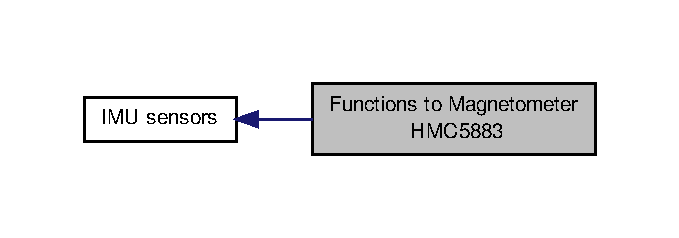
\includegraphics[width=326pt]{group__mag}
\end{center}
\end{figure}
\subsection*{Functions}
\begin{DoxyCompactItemize}
\item 
uint8\-\_\-t $\ast$ \hyperlink{group__mag_ga6830eaeae2298320e1e8c902e4edd709}{mag\-\_\-read\-\_\-reg} (int \hyperlink{CommunicationV0_2communication_8c_a7751bd45ac1064efb35adf1f19c25db8}{i2c\-\_\-dev}, uint8\-\_\-t reg, uint8\-\_\-t count)
\begin{DoxyCompactList}\small\item\em R\-E\-A\-D C\-O\-U\-N\-T 8-\/\-B\-I\-T R\-E\-G\-I\-S\-T\-E\-R I\-N S\-E\-Q\-U\-E\-N\-C\-E. \end{DoxyCompactList}\item 
int \hyperlink{group__mag_gab42ae0d0a2a6f37cf36d856c072b7f34}{mag\-\_\-read\-\_\-all\-\_\-data} (int \hyperlink{CommunicationV0_2communication_8c_a7751bd45ac1064efb35adf1f19c25db8}{i2c\-\_\-dev}, short int $\ast$data)
\begin{DoxyCompactList}\small\item\em R\-E\-A\-D A\-L\-L D\-A\-T\-A A\-T O\-N\-C\-E (X, Y and Z) \end{DoxyCompactList}\item 
short int \hyperlink{group__mag_ga542a31ccd07cd2c3e8e2b68cdb6d219e}{mag\-\_\-read\-\_\-data} (int \hyperlink{CommunicationV0_2communication_8c_a7751bd45ac1064efb35adf1f19c25db8}{i2c\-\_\-dev}, int axis)
\begin{DoxyCompactList}\small\item\em R\-E\-A\-D D\-A\-T\-A (X, Y or Z) \end{DoxyCompactList}\end{DoxyCompactItemize}


\subsection{Detailed Description}


\subsection{Function Documentation}
\hypertarget{group__mag_gab42ae0d0a2a6f37cf36d856c072b7f34}{\index{Functions to Magnetometer H\-M\-C5883@{Functions to Magnetometer H\-M\-C5883}!mag\-\_\-read\-\_\-all\-\_\-data@{mag\-\_\-read\-\_\-all\-\_\-data}}
\index{mag\-\_\-read\-\_\-all\-\_\-data@{mag\-\_\-read\-\_\-all\-\_\-data}!Functions to Magnetometer HMC5883@{Functions to Magnetometer H\-M\-C5883}}
\subsubsection[{mag\-\_\-read\-\_\-all\-\_\-data}]{\setlength{\rightskip}{0pt plus 5cm}int mag\-\_\-read\-\_\-all\-\_\-data (
\begin{DoxyParamCaption}
\item[{int}]{i2c\-\_\-dev, }
\item[{short int $\ast$}]{data}
\end{DoxyParamCaption}
)}}\label{group__mag_gab42ae0d0a2a6f37cf36d856c072b7f34}


R\-E\-A\-D A\-L\-L D\-A\-T\-A A\-T O\-N\-C\-E (X, Y and Z) 


\begin{DoxyParams}[1]{Parameters}
 & {\em i2c\-\_\-dev} & \\
\hline
\mbox{\tt out}  & {\em $\ast$data} & \\
\hline
\end{DoxyParams}


Definition at line 121 of file mag\-\_\-functions.\-c.



Referenced by read\-\_\-all\-\_\-data().


\begin{DoxyCode}
122 \{
123   uint8\_t i, j;
124   uint8\_t *data8;
125   \textcolor{keyword}{union }result
126   \{
127     \textcolor{keywordtype}{unsigned} \textcolor{keywordtype}{short} \textcolor{keywordtype}{int} usgnd[3];
128     \textcolor{keywordtype}{short} \textcolor{keywordtype}{int} sgnd[3];
129   \} result;
130   \textcolor{comment}{//result=(union result*)malloc(3*sizeof(union result));}
131   \textcolor{keywordflow}{if}( (data8=\hyperlink{group__mag_ga6830eaeae2298320e1e8c902e4edd709}{mag\_read\_reg}(\hyperlink{CommunicationV0_2communication_8c_a7751bd45ac1064efb35adf1f19c25db8}{i2c\_dev},\hyperlink{communication_2imu__regs_8h_a4f883328e7ae117996e334145ddd0032}{MAG\_DATAX1},6))==NULL)
132   \{
133     \textcolor{comment}{//perror("Read accelerometer register failed");}
134     \textcolor{keywordflow}{return} \hyperlink{calibration_2calibration_8h_a6d58f9ac447476b4e084d7ca383f5183}{FAILURE};
135   \}
136   \textcolor{comment}{//result.usgnd=(unsigned int*)malloc(3*sizeof(unsigned int));}
137   j=0;
138   \textcolor{keywordflow}{for}(i=0; i<3; i++)
139   \{
140     result.usgnd[j]=0;
141     result.usgnd[j]=result.usgnd[j]|((\textcolor{keywordtype}{unsigned} \textcolor{keywordtype}{short} int)data8[i*2+1])|(((\textcolor{keywordtype}{unsigned} int)data8[i*2])<<8);
142     data[j]=result.sgnd[j];
143     j=2-i; \textcolor{comment}{// trick used to change the sorting of the data from XZY to XYZ}
144   \}
145   \textcolor{keywordflow}{return} \hyperlink{calibration_2calibration_8h_aa90cac659d18e8ef6294c7ae337f6b58}{SUCCESS};  
146 \}
\end{DoxyCode}


Here is the caller graph for this function\-:
\nopagebreak
\begin{figure}[H]
\begin{center}
\leavevmode
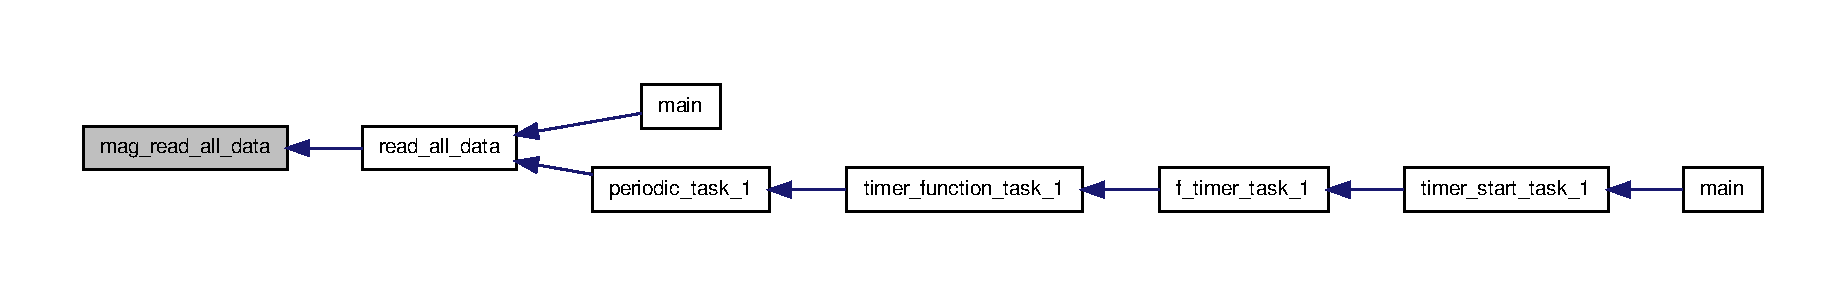
\includegraphics[width=350pt]{group__mag_gab42ae0d0a2a6f37cf36d856c072b7f34_icgraph}
\end{center}
\end{figure}


\hypertarget{group__mag_ga542a31ccd07cd2c3e8e2b68cdb6d219e}{\index{Functions to Magnetometer H\-M\-C5883@{Functions to Magnetometer H\-M\-C5883}!mag\-\_\-read\-\_\-data@{mag\-\_\-read\-\_\-data}}
\index{mag\-\_\-read\-\_\-data@{mag\-\_\-read\-\_\-data}!Functions to Magnetometer HMC5883@{Functions to Magnetometer H\-M\-C5883}}
\subsubsection[{mag\-\_\-read\-\_\-data}]{\setlength{\rightskip}{0pt plus 5cm}short int mag\-\_\-read\-\_\-data (
\begin{DoxyParamCaption}
\item[{int}]{i2c\-\_\-dev, }
\item[{int}]{axis}
\end{DoxyParamCaption}
)}}\label{group__mag_ga542a31ccd07cd2c3e8e2b68cdb6d219e}


R\-E\-A\-D D\-A\-T\-A (X, Y or Z) 


\begin{DoxyParams}{Parameters}
{\em i2c\-\_\-dev} & \\
\hline
{\em axis} & set the axis ('X' or 'Y' or 'Z') \\
\hline
\end{DoxyParams}


Definition at line 148 of file mag\-\_\-functions.\-c.


\begin{DoxyCode}
149 \{
150   uint8\_t *data;
151   \textcolor{keyword}{union }result
152   \{
153     \textcolor{keywordtype}{unsigned} \textcolor{keywordtype}{int} usgnd;
154     \textcolor{keywordtype}{int} sgnd;
155   \}result;
156 
157   \textcolor{keywordflow}{switch}(axis)\{
158     \textcolor{keywordflow}{case} \textcolor{charliteral}{'X'}:
159       data=\hyperlink{group__mag_ga6830eaeae2298320e1e8c902e4edd709}{mag\_read\_reg}(\hyperlink{CommunicationV0_2communication_8c_a7751bd45ac1064efb35adf1f19c25db8}{i2c\_dev},\hyperlink{communication_2imu__regs_8h_a4f883328e7ae117996e334145ddd0032}{MAG\_DATAX1},2);
160       \textcolor{keywordflow}{break};
161     \textcolor{keywordflow}{case} \textcolor{charliteral}{'Y'}:
162       data=\hyperlink{group__mag_ga6830eaeae2298320e1e8c902e4edd709}{mag\_read\_reg}(\hyperlink{CommunicationV0_2communication_8c_a7751bd45ac1064efb35adf1f19c25db8}{i2c\_dev},\hyperlink{communication_2imu__regs_8h_ae218906702b1e40c2b6970f97dd0cfe4}{MAG\_DATAY1},2);
163       \textcolor{keywordflow}{break};
164     \textcolor{keywordflow}{case} \textcolor{charliteral}{'Z'}:
165       data=\hyperlink{group__mag_ga6830eaeae2298320e1e8c902e4edd709}{mag\_read\_reg}(\hyperlink{CommunicationV0_2communication_8c_a7751bd45ac1064efb35adf1f19c25db8}{i2c\_dev},\hyperlink{communication_2imu__regs_8h_a81d7d9236ec69a1a229e4fa7c6299fde}{MAG\_DATAZ1},2);
166       \textcolor{keywordflow}{break};
167     \textcolor{keywordflow}{default}:
168       \textcolor{comment}{//perror("Wrong argument for axis in mag\_read\_data");}
169       \textcolor{keywordflow}{return} -1;
170   \}
171   result.usgnd=0;
172   result.usgnd=result.usgnd|(((\textcolor{keywordtype}{unsigned} \textcolor{keywordtype}{short} int)data[1]))|(((\textcolor{keywordtype}{unsigned} \textcolor{keywordtype}{short} \textcolor{keywordtype}{int})data[0])<<8);
173   \textcolor{keywordflow}{return} result.sgnd;
174 \}
\end{DoxyCode}
\hypertarget{group__mag_ga6830eaeae2298320e1e8c902e4edd709}{\index{Functions to Magnetometer H\-M\-C5883@{Functions to Magnetometer H\-M\-C5883}!mag\-\_\-read\-\_\-reg@{mag\-\_\-read\-\_\-reg}}
\index{mag\-\_\-read\-\_\-reg@{mag\-\_\-read\-\_\-reg}!Functions to Magnetometer HMC5883@{Functions to Magnetometer H\-M\-C5883}}
\subsubsection[{mag\-\_\-read\-\_\-reg}]{\setlength{\rightskip}{0pt plus 5cm}uint8\-\_\-t$\ast$ mag\-\_\-read\-\_\-reg (
\begin{DoxyParamCaption}
\item[{int}]{i2c\-\_\-dev, }
\item[{uint8\-\_\-t}]{reg, }
\item[{uint8\-\_\-t}]{count}
\end{DoxyParamCaption}
)}}\label{group__mag_ga6830eaeae2298320e1e8c902e4edd709}


R\-E\-A\-D C\-O\-U\-N\-T 8-\/\-B\-I\-T R\-E\-G\-I\-S\-T\-E\-R I\-N S\-E\-Q\-U\-E\-N\-C\-E. 


\begin{DoxyParams}{Parameters}
{\em i2c\-\_\-dev} & \\
\hline
{\em reg} & \\
\hline
{\em count} & number of registers in sequence (1-\/13) \\
\hline
\end{DoxyParams}


Definition at line 31 of file mag\-\_\-functions.\-c.



Referenced by mag\-\_\-read\-\_\-all\-\_\-data(), and mag\-\_\-read\-\_\-data().


\begin{DoxyCode}
32 \{
33   uint8\_t data[13];
34   \textcolor{keywordtype}{int} i;
35 
36   \textcolor{comment}{//data=(uint8\_t*)malloc((count+1)*sizeof(data));}
37   
38   data[0] = reg;
39 
40   \textcolor{keywordflow}{if} (write(\hyperlink{CommunicationV0_2communication_8c_a7751bd45ac1064efb35adf1f19c25db8}{i2c\_dev}, &data, 1) != 1) \{            
41         \textcolor{comment}{//perror("write before read");}
42         \textcolor{keywordflow}{return} NULL;
43   \}
44   data[0] = 0;
45   \textcolor{keywordflow}{if} (read(\hyperlink{CommunicationV0_2communication_8c_a7751bd45ac1064efb35adf1f19c25db8}{i2c\_dev}, &data, count) != count) \{
46         \textcolor{comment}{//perror("read");}
47         \textcolor{keywordflow}{return} NULL;    
48   \}
49 
50   \textcolor{keywordflow}{return} data;
51 \}
\end{DoxyCode}


Here is the caller graph for this function\-:\nopagebreak
\begin{figure}[H]
\begin{center}
\leavevmode
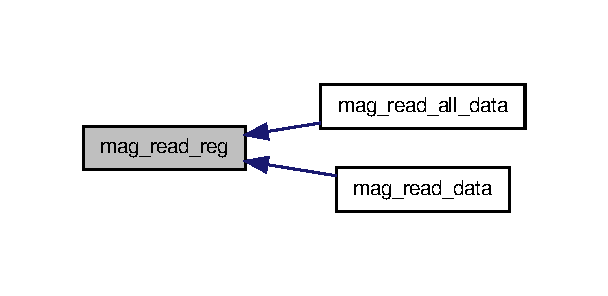
\includegraphics[width=292pt]{group__mag_ga6830eaeae2298320e1e8c902e4edd709_icgraph}
\end{center}
\end{figure}



\hypertarget{group__mainConfig}{\section{Configuration of the main}
\label{group__mainConfig}\index{Configuration of the main@{Configuration of the main}}
}
\subsection*{Macros}
\begin{DoxyCompactItemize}
\item 
\#define \hyperlink{group__mainConfig_ga745f0e5078faacf33bffbc94239f62a9}{T\-A\-S\-K1\-\_\-\-P\-E\-R\-I\-O\-D}~100
\end{DoxyCompactItemize}


\subsection{Detailed Description}


\subsection{Macro Definition Documentation}
\hypertarget{group__mainConfig_ga745f0e5078faacf33bffbc94239f62a9}{\index{Configuration of the main@{Configuration of the main}!T\-A\-S\-K1\-\_\-\-P\-E\-R\-I\-O\-D@{T\-A\-S\-K1\-\_\-\-P\-E\-R\-I\-O\-D}}
\index{T\-A\-S\-K1\-\_\-\-P\-E\-R\-I\-O\-D@{T\-A\-S\-K1\-\_\-\-P\-E\-R\-I\-O\-D}!Configuration of the main@{Configuration of the main}}
\subsubsection[{T\-A\-S\-K1\-\_\-\-P\-E\-R\-I\-O\-D}]{\setlength{\rightskip}{0pt plus 5cm}\#define T\-A\-S\-K1\-\_\-\-P\-E\-R\-I\-O\-D~100}}\label{group__mainConfig_ga745f0e5078faacf33bffbc94239f62a9}


Definition at line 16 of file main.\-h.


\hypertarget{group__taskS}{\section{Scheduler for tasks}
\label{group__taskS}\index{Scheduler for tasks@{Scheduler for tasks}}
}


Implentation of Scheduler for tasks\-:  


\subsection*{Functions}
\begin{DoxyCompactItemize}
\item 
void \hyperlink{group__taskS_gaf56f9692a592fdc4b0f74aaac3b76168}{timer\-\_\-new\-\_\-task} (\hyperlink{structTASK__S}{T\-A\-S\-K\-\_\-\-S} $\ast$task, timer\-\_\-t timer, void $\ast$run\-Funtion)
\begin{DoxyCompactList}\small\item\em Create a task. \end{DoxyCompactList}\item 
void \hyperlink{group__taskS_gac088a054258396a6e2dba77908f22b42}{timer\-\_\-start\-\_\-task} (\hyperlink{structTASK__S}{T\-A\-S\-K\-\_\-\-S} $\ast$task)
\begin{DoxyCompactList}\small\item\em Start some task. \end{DoxyCompactList}\item 
void \hyperlink{group__taskS_ga8e48eacaac7d9cf7d82cc71cfbcd4b56}{timer\-\_\-stop\-\_\-task} (\hyperlink{structTASK__S}{T\-A\-S\-K\-\_\-\-S} $\ast$task)
\begin{DoxyCompactList}\small\item\em Stop some task. \end{DoxyCompactList}\end{DoxyCompactItemize}


\subsection{Detailed Description}
Implentation of Scheduler for tasks\-: \begin{DoxyAuthor}{Author}
Rafael 
\end{DoxyAuthor}
\begin{DoxyRefDesc}{Todo}
\item[\hyperlink{todo__todo000004}{Todo}]test it \end{DoxyRefDesc}


\subsection{Function Documentation}
\hypertarget{group__taskS_gaf56f9692a592fdc4b0f74aaac3b76168}{\index{Scheduler for tasks@{Scheduler for tasks}!timer\-\_\-new\-\_\-task@{timer\-\_\-new\-\_\-task}}
\index{timer\-\_\-new\-\_\-task@{timer\-\_\-new\-\_\-task}!Scheduler for tasks@{Scheduler for tasks}}
\subsubsection[{timer\-\_\-new\-\_\-task}]{\setlength{\rightskip}{0pt plus 5cm}void timer\-\_\-new\-\_\-task (
\begin{DoxyParamCaption}
\item[{{\bf T\-A\-S\-K\-\_\-\-S} $\ast$}]{task, }
\item[{timer\-\_\-t}]{timer, }
\item[{void $\ast$}]{run\-Funtion}
\end{DoxyParamCaption}
)}}\label{group__taskS_gaf56f9692a592fdc4b0f74aaac3b76168}


Create a task. 


\begin{DoxyParams}{Parameters}
{\em $\ast$task} & \\
\hline
{\em $\ast$void\-Function} & Pointer to the function called to execute \\
\hline
\end{DoxyParams}
\hypertarget{group__taskS_gac088a054258396a6e2dba77908f22b42}{\index{Scheduler for tasks@{Scheduler for tasks}!timer\-\_\-start\-\_\-task@{timer\-\_\-start\-\_\-task}}
\index{timer\-\_\-start\-\_\-task@{timer\-\_\-start\-\_\-task}!Scheduler for tasks@{Scheduler for tasks}}
\subsubsection[{timer\-\_\-start\-\_\-task}]{\setlength{\rightskip}{0pt plus 5cm}void timer\-\_\-start\-\_\-task (
\begin{DoxyParamCaption}
\item[{{\bf T\-A\-S\-K\-\_\-\-S} $\ast$}]{task}
\end{DoxyParamCaption}
)}}\label{group__taskS_gac088a054258396a6e2dba77908f22b42}


Start some task. 



Definition at line 18 of file task\-Scheduler.\-c.



References f\-\_\-timer\-\_\-task\-\_\-1().



Referenced by main().


\begin{DoxyCode}
18                                    \{
19   \textcolor{keyword}{struct }itimerspec itimer;
20   \textcolor{keyword}{struct }sigevent sigev;
21   \textcolor{keywordtype}{int} erno = 0;
22 
23   (*task).isFirstExecution = 1;
24 
25   itimer.it\_interval.tv\_sec = 0;
26   itimer.it\_interval.tv\_nsec= (*task).period\_us*1000;
27   itimer.it\_value = itimer.it\_interval;
28 
29   memset(&sigev,0,\textcolor{keyword}{sizeof}(\textcolor{keyword}{struct} sigevent));
30 
31   sigev.sigev\_value.sival\_int = 0;
32   sigev.sigev\_notify = SIGEV\_THREAD;
33   sigev.sigev\_notify\_attributes = NULL;
34   sigev.sigev\_notify\_function = \hyperlink{main2_8c_a5ce2b6a7dd4d00c90fe18098091044aa}{f\_timer\_task\_1};
35 
36   \textcolor{keywordflow}{if} (timer\_create(CLOCK\_REALTIME, &sigev, &((*task).timer)) < 0)
37   \{
38     fprintf(stderr, \textcolor{stringliteral}{"[%d]: %s\(\backslash\)n"}, \_\_LINE\_\_, strerror(erno));
39     exit(erno);
40   \}
41 
42   \textcolor{keywordflow}{if}(timer\_settime((*task).timer,0,&itimer,NULL) < 0)
43   \{
44     fprintf(stderr,\textcolor{stringliteral}{"[%d]: %s\(\backslash\)n"}, \_\_LINE\_\_, strerror(erno));
45     exit(erno);
46   \}
47 \}
\end{DoxyCode}


Here is the call graph for this function\-:\nopagebreak
\begin{figure}[H]
\begin{center}
\leavevmode
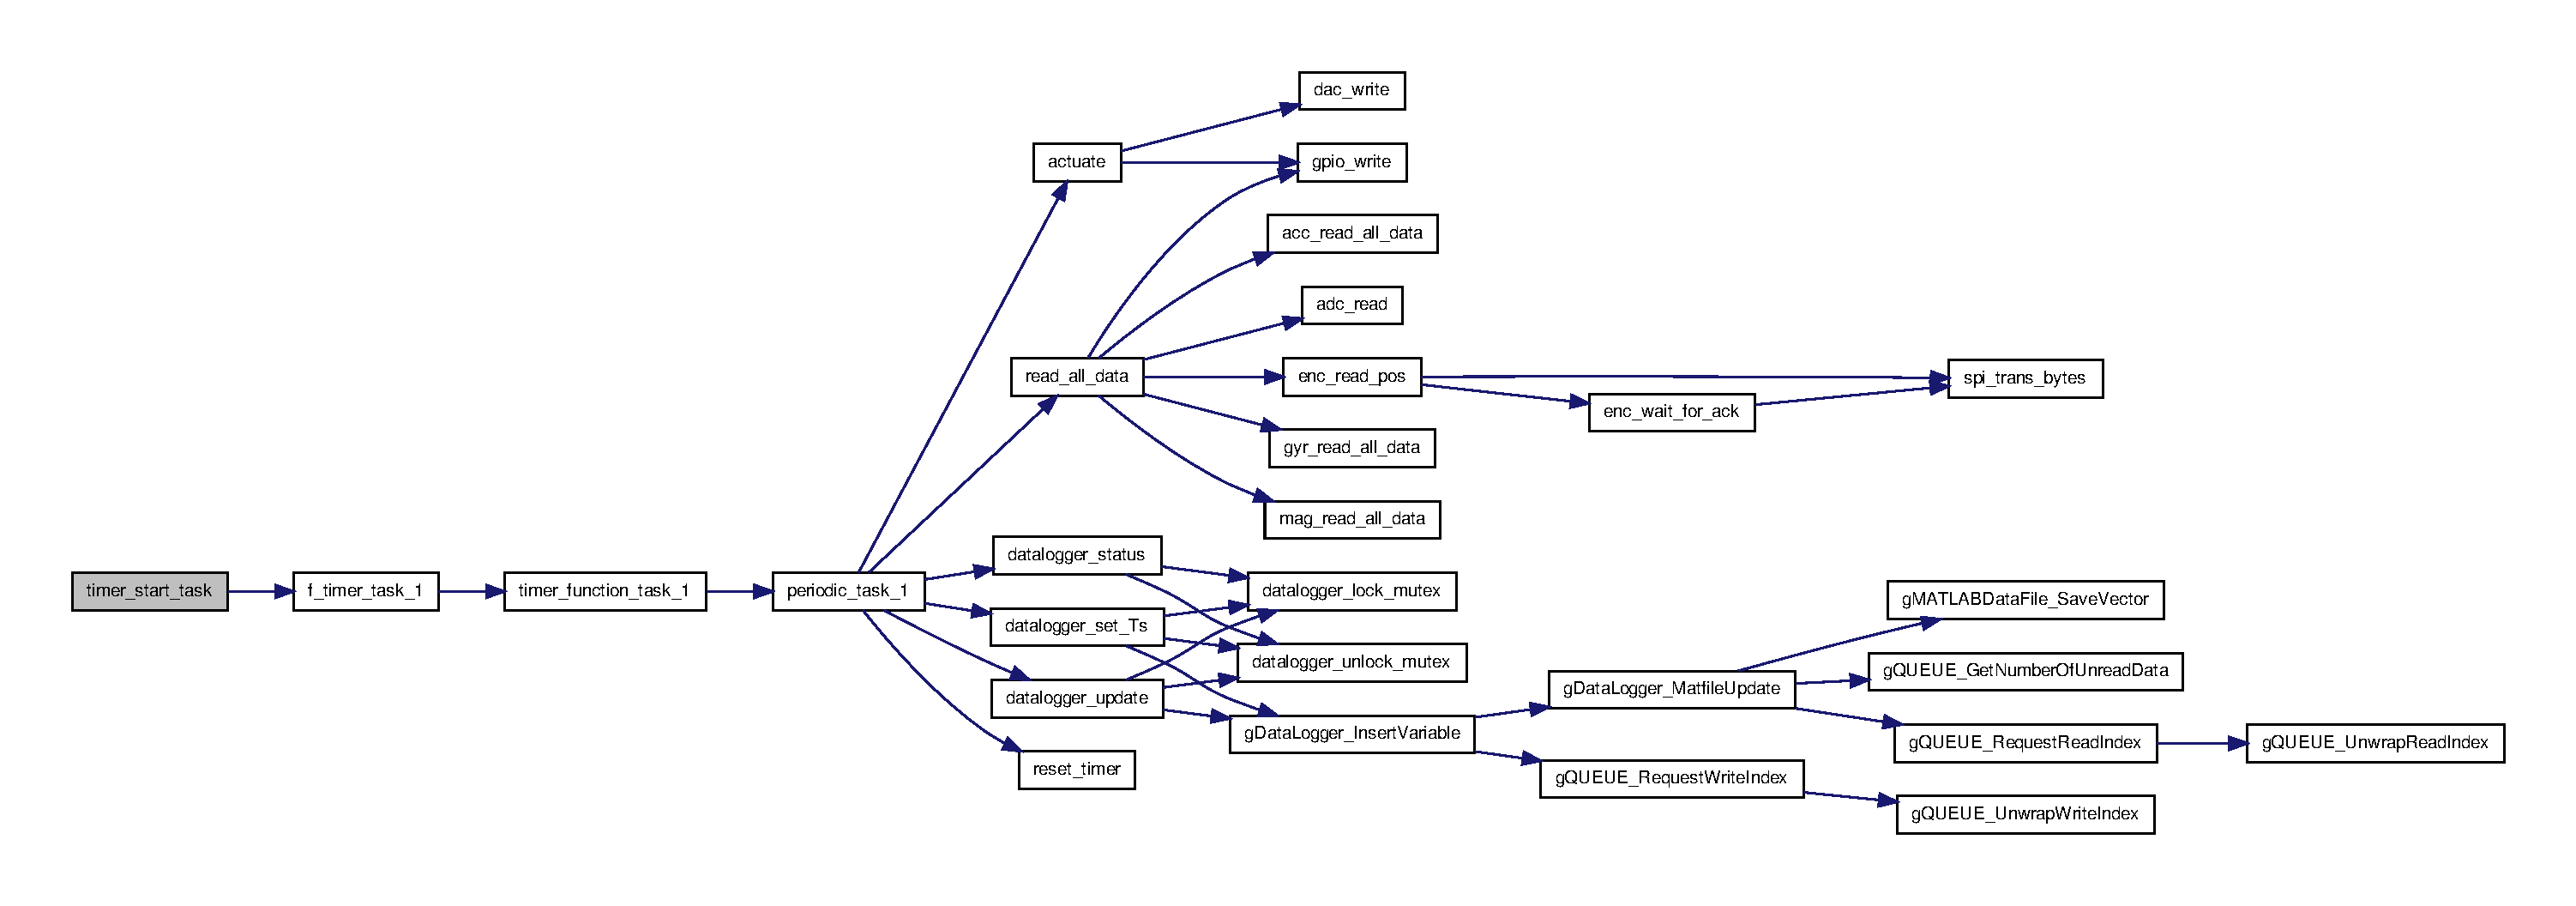
\includegraphics[width=350pt]{group__taskS_gac088a054258396a6e2dba77908f22b42_cgraph}
\end{center}
\end{figure}




Here is the caller graph for this function\-:
\nopagebreak
\begin{figure}[H]
\begin{center}
\leavevmode
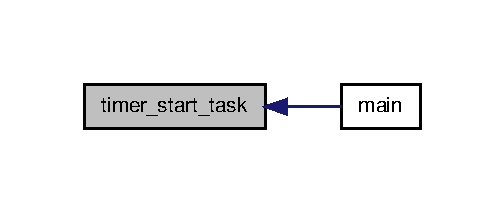
\includegraphics[width=242pt]{group__taskS_gac088a054258396a6e2dba77908f22b42_icgraph}
\end{center}
\end{figure}


\hypertarget{group__taskS_ga8e48eacaac7d9cf7d82cc71cfbcd4b56}{\index{Scheduler for tasks@{Scheduler for tasks}!timer\-\_\-stop\-\_\-task@{timer\-\_\-stop\-\_\-task}}
\index{timer\-\_\-stop\-\_\-task@{timer\-\_\-stop\-\_\-task}!Scheduler for tasks@{Scheduler for tasks}}
\subsubsection[{timer\-\_\-stop\-\_\-task}]{\setlength{\rightskip}{0pt plus 5cm}void timer\-\_\-stop\-\_\-task (
\begin{DoxyParamCaption}
\item[{{\bf T\-A\-S\-K\-\_\-\-S} $\ast$}]{task}
\end{DoxyParamCaption}
)}}\label{group__taskS_ga8e48eacaac7d9cf7d82cc71cfbcd4b56}


Stop some task. 

\begin{DoxyRefDesc}{Todo}
\item[\hyperlink{todo__todo000005}{Todo}]verify use of variable 'erno' \end{DoxyRefDesc}


Definition at line 102 of file task\-Scheduler.\-c.



Referenced by main().


\begin{DoxyCode}
102                                   \{
103   \textcolor{keywordtype}{int} erno = 0;
104   \textcolor{keywordflow}{if}(timer\_delete((*task).timer)<0)\{
105     fprintf(stderr,\textcolor{stringliteral}{"[%d]:%s\(\backslash\)n"},\_\_LINE\_\_,strerror(erno));
106     exit(erno);
107   \}
108 \}
\end{DoxyCode}


Here is the caller graph for this function\-:
\nopagebreak
\begin{figure}[H]
\begin{center}
\leavevmode
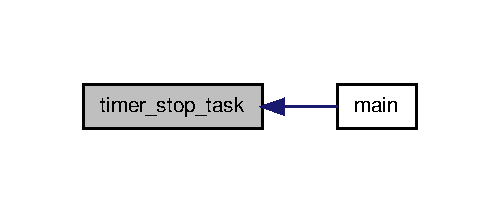
\includegraphics[width=240pt]{group__taskS_ga8e48eacaac7d9cf7d82cc71cfbcd4b56_icgraph}
\end{center}
\end{figure}



\hypertarget{group__ui}{
\section{Functions to deal the User Inteface using ncurses}
\label{group__ui}\index{Functions to deal the User Inteface using ncurses@{Functions to deal the User Inteface using ncurses}}
}
\subsection*{Functions}
\begin{DoxyCompactItemize}
\item 
int \hyperlink{group__ui_gab7bfb453918dcc296ff0cea3c79453d0}{ui\_\-init} (void)
\begin{DoxyCompactList}\small\item\em Initialize UI. \item\end{DoxyCompactList}\item 
int \hyperlink{group__ui_ga65d8b92b634da17c344458cd57e61f3e}{ui\_\-close} (void)
\begin{DoxyCompactList}\small\item\em Close UI. \item\end{DoxyCompactList}\item 
int \hyperlink{group__ui_ga42e4dac2d138061a74c572358c8ebf49}{ui\_\-update} (\hyperlink{structIMU__DATA__STRUCT}{IMU\_\-DATA\_\-STRUCT} $\ast$pimu\_\-data, \hyperlink{structEFF__DATA__STRUCT}{EFF\_\-DATA\_\-STRUCT} $\ast$peff\_\-data, \hyperlink{structMRA__DATA__STRUCT}{MRA\_\-DATA\_\-STRUCT} $\ast$pmra\_\-data, \hyperlink{structENC__DATA__STRUCT}{ENC\_\-DATA\_\-STRUCT} $\ast$\hyperlink{main2_8c_aaa441e18ae805c4f3efb0b5231d1cfe7}{enc\_\-data}, int \hyperlink{threads__linux_8c_ac7af894858cf396a219d632f40afdc8d}{total}, int \hyperlink{threads__linux_8c_a4f35e5ea2395561d0bd3b2f45612dc2c}{failure})
\begin{DoxyCompactList}\small\item\em Update Screen with new data of sensors. \item\end{DoxyCompactList}\item 
int \hyperlink{group__ui_ga7d5a9d9a75693709de408781d001a6a6}{ui\_\-imu\_\-data} (\hyperlink{structIMU__DATA__STRUCT}{IMU\_\-DATA\_\-STRUCT} $\ast$pimu\_\-data)
\begin{DoxyCompactList}\small\item\em Print IMU data. \item\end{DoxyCompactList}\item 
int \hyperlink{group__ui_gaefec243c5df45db0350c1abbccf20e3b}{ui\_\-mra\_\-data} (\hyperlink{structMRA__DATA__STRUCT}{MRA\_\-DATA\_\-STRUCT} $\ast$pmra\_\-data)
\begin{DoxyCompactList}\small\item\em Print MRA data. \item\end{DoxyCompactList}\end{DoxyCompactItemize}


\subsection{Function Documentation}
\hypertarget{group__ui_ga65d8b92b634da17c344458cd57e61f3e}{
\index{ui@{ui}!ui\_\-close@{ui\_\-close}}
\index{ui\_\-close@{ui\_\-close}!ui@{ui}}
\subsubsection[{ui\_\-close}]{\setlength{\rightskip}{0pt plus 5cm}int ui\_\-close (void)}}
\label{group__ui_ga65d8b92b634da17c344458cd57e61f3e}


Close UI. 



Definition at line 41 of file ui.c.



References SUCCESS.



Referenced by main(), and threads\_\-linux\_\-init().




\begin{DoxyCode}
42 {
43     #if UI_MODULE_ENABLED
44         clear();
45         printw("Cleaning up...\n");
46         refresh();
47         endwin();
48     #endif
49 
50           return SUCCESS;
51 }
\end{DoxyCode}




Here is the caller graph for this function:

\hypertarget{group__ui_ga7d5a9d9a75693709de408781d001a6a6}{
\index{ui@{ui}!ui\_\-imu\_\-data@{ui\_\-imu\_\-data}}
\index{ui\_\-imu\_\-data@{ui\_\-imu\_\-data}!ui@{ui}}
\subsubsection[{ui\_\-imu\_\-data}]{\setlength{\rightskip}{0pt plus 5cm}int ui\_\-imu\_\-data ({\bf IMU\_\-DATA\_\-STRUCT} $\ast$ {\em pimu\_\-data})}}
\label{group__ui_ga7d5a9d9a75693709de408781d001a6a6}


Print IMU data. 



Definition at line 130 of file ui.c.



References IMU\_\-DATA\_\-STRUCT::calibrated::acc, IMU\_\-DATA\_\-STRUCT::acc, IMU\_\-DATA\_\-STRUCT::calib, IMU\_\-DATA\_\-STRUCT::calibrated::gyr, IMU\_\-DATA\_\-STRUCT::gyr, IMU\_\-DATA\_\-STRUCT::calibrated::mag, IMU\_\-DATA\_\-STRUCT::mag, SUCCESS, DATA\_\-XYZ\_\-DOUBLE::x, DATA\_\-XYZ::x, DATA\_\-XYZ\_\-DOUBLE::y, DATA\_\-XYZ::y, DATA\_\-XYZ\_\-DOUBLE::z, and DATA\_\-XYZ::z.



Referenced by ui\_\-update().




\begin{DoxyCode}
131 {
132         mvprintw(2, 0, "Accelerometer X (raw): %d", pimu_data->acc.x);
133         mvprintw(2, 40, "Accelerometer X (g): %lf", pimu_data->calib.acc.x);
134         mvprintw(3, 0, "Accelerometer Y (raw): %d", pimu_data->acc.y);
135         mvprintw(3, 40, "Accelerometer Y (g): %lf", pimu_data->calib.acc.y);
136         mvprintw(4, 0, "Accelerometer Z (raw): %d", pimu_data->acc.z);
137         mvprintw(4, 40, "Accelerometer Z (g): %lf", pimu_data->calib.acc.z);
138         mvprintw(5, 0, "Gyrometer X (raw):     %d", pimu_data->gyr.x);
139         mvprintw(5, 40, "Gyrometer X (rad/sec):   %lf", pimu_data->calib.gyr.x);
140         mvprintw(6, 0, "Gyrometer Y (raw):     %d", pimu_data->gyr.y);
141         mvprintw(6, 40, "Gyrometer Y (rad/sec):   %lf", pimu_data->calib.gyr.y);
142         mvprintw(7, 0, "Gyrometer Z (raw):     %d", pimu_data->gyr.z);
143         mvprintw(7, 40, "Gyrometer Z (rad/sec):   %lf", pimu_data->calib.gyr.z);
144         mvprintw(8, 0, "Magnetometer X (raw):  %d", pimu_data->mag.x);
145         mvprintw(8, 40, "Magnetometer X (B):     %lf", pimu_data->calib.mag.x);
146         mvprintw(9, 0, "Magnetometer Y (raw):  %d", pimu_data->mag.y);
147         mvprintw(9, 40, "Magnetometer Y (B):     %lf", pimu_data->calib.mag.y);
148         mvprintw(10,0, "Magnetometer Z (raw):  %d", pimu_data->mag.z);
149         mvprintw(10,40, "Magnetometer Z (B):     %lf", pimu_data->calib.mag.z);
150         mvprintw(12,0,"Total Acceleromter: %lf",sqrt(pimu_data->calib.acc.x*pimu_
      data->calib.acc.x+pimu_data->calib.acc.y*pimu_data->calib.acc.y+pimu_data->calib.
      acc.z*pimu_data->calib.acc.z));
151         mvprintw(13,0,"Total Gyrometer: %lf",sqrt(pimu_data->calib.gyr.x*pimu_dat
      a->calib.gyr.x+pimu_data->calib.gyr.y*pimu_data->calib.gyr.y+pimu_data->calib.
      gyr.z*pimu_data->calib.gyr.z));
152         mvprintw(14,0,"Total Magnetometer: %lf",sqrt(pimu_data->calib.mag.x*pimu_
      data->calib.mag.x+pimu_data->calib.mag.y*pimu_data->calib.mag.y+pimu_data->calib.
      mag.z*pimu_data->calib.mag.z));
153         //mvprintw(15, 0, "Encoder (raw): %lf", enc.data);
154 
155         return SUCCESS;
156 }
\end{DoxyCode}




Here is the caller graph for this function:

\hypertarget{group__ui_gab7bfb453918dcc296ff0cea3c79453d0}{
\index{ui@{ui}!ui\_\-init@{ui\_\-init}}
\index{ui\_\-init@{ui\_\-init}!ui@{ui}}
\subsubsection[{ui\_\-init}]{\setlength{\rightskip}{0pt plus 5cm}int ui\_\-init (void)}}
\label{group__ui_gab7bfb453918dcc296ff0cea3c79453d0}


Initialize UI. 



Definition at line 26 of file ui.c.



References SUCCESS, and TRUE.



Referenced by main(), and threads\_\-linux\_\-init().




\begin{DoxyCode}
27 {
28     #if UI_MODULE_ENABLED
29         //NCURSES
30         initscr();
31         scrollok(stdscr,TRUE);
32         //resizeterm(33,100);
33         //wresize(scr,32,100);
34         //erase();
35         timeout(0); //No delay for getch();
36     #endif
37 
38         return SUCCESS;
39 }
\end{DoxyCode}




Here is the caller graph for this function:

\hypertarget{group__ui_gaefec243c5df45db0350c1abbccf20e3b}{
\index{ui@{ui}!ui\_\-mra\_\-data@{ui\_\-mra\_\-data}}
\index{ui\_\-mra\_\-data@{ui\_\-mra\_\-data}!ui@{ui}}
\subsubsection[{ui\_\-mra\_\-data}]{\setlength{\rightskip}{0pt plus 5cm}int ui\_\-mra\_\-data ({\bf MRA\_\-DATA\_\-STRUCT} $\ast$ {\em pmra\_\-data})}}
\label{group__ui_gaefec243c5df45db0350c1abbccf20e3b}


Print MRA data. 



Definition at line 183 of file ui.c.



References SUCCESS, MRA\_\-DATA\_\-STRUCT::v\_\-ctl, and MRA\_\-DATA\_\-STRUCT::v\_\-ctl\_\-read.



Referenced by ui\_\-update().




\begin{DoxyCode}
184 {
185         mvprintw(2,0,"V_ctl (bits): %d",pmra_data->v_ctl);
186         mvprintw(3,0,"V_ctl_read (bits): %d",pmra_data->v_ctl_read);
187         //mvprintw(2,40,"Fx (N): %lf",peff_data->??);
188 
189         return SUCCESS;
190 }
\end{DoxyCode}




Here is the caller graph for this function:

\hypertarget{group__ui_ga42e4dac2d138061a74c572358c8ebf49}{
\index{ui@{ui}!ui\_\-update@{ui\_\-update}}
\index{ui\_\-update@{ui\_\-update}!ui@{ui}}
\subsubsection[{ui\_\-update}]{\setlength{\rightskip}{0pt plus 5cm}int ui\_\-update ({\bf IMU\_\-DATA\_\-STRUCT} $\ast$ {\em pimu\_\-data}, \/  {\bf EFF\_\-DATA\_\-STRUCT} $\ast$ {\em peff\_\-data}, \/  {\bf MRA\_\-DATA\_\-STRUCT} $\ast$ {\em pmra\_\-data}, \/  {\bf ENC\_\-DATA\_\-STRUCT} $\ast$ {\em enc\_\-data}, \/  int {\em total}, \/  int {\em failure})}}
\label{group__ui_ga42e4dac2d138061a74c572358c8ebf49}


Update Screen with new data of sensors. 



Definition at line 53 of file ui.c.



References exit\_\-program(), FAILURE, SUCCESS, ui\_\-eff\_\-data(), ui\_\-enc\_\-data(), ui\_\-imu\_\-data(), ui\_\-mra\_\-data(), and ui\_\-overview\_\-data().



Referenced by periodic\_\-task\_\-2(), threads\_\-linux\_\-periodic\_\-task\_\-2(), and ui\_\-task().




\begin{DoxyCode}
54 {
55         unsigned char user_char = 0;
56 
57         static enum {UI_OVERVIEW = 0, UI_IMU, UI_EFF, UI_MRA , UI_ENC} ui_state;
58 
59         erase();
60         //wresize(scr,32,100);
61         attron(A_STANDOUT);
62 
63         mvaddstr(0,15,"RLEG Data");
64         attroff(A_STANDOUT);
65 
66         switch(ui_state)
67         {
68                 case UI_IMU:
69                         if(ui_imu_data(pimu_data) != SUCCESS) return FAILURE;
70                         break;
71                 case UI_EFF:
72                         if(ui_eff_data(peff_data) != SUCCESS) return FAILURE;
73                         break;
74                 case UI_MRA:
75                         if(ui_mra_data(pmra_data) != SUCCESS) return FAILURE;
76                         break;
77         case UI_ENC:
78                         if(ui_enc_data(enc_data) != SUCCESS) return FAILURE;
79                         break;
80                 case UI_OVERVIEW:
81                 default:
82                         if(ui_overview_data(total, failure, pimu_data, peff_data,
       pmra_data, enc_data) != SUCCESS) return FAILURE;
83                         break;
84         }
85 
86         refresh();
87 
88         user_char = getch(); //Getting a char typed by the user
89         switch(user_char)
90         {
91                 case 'Q':
92                 case 'q': //Quit
93                         exit_program();
94                         break;
95                 case 'i': //IMU view
96                         ui_state = UI_IMU;
97                         break;
98                 case 'f': //EFF view
99                         ui_state = UI_EFF;
100                         break;
101             case 'e': // ENCODER view
102                     ui_state = UI_ENC;
103                     break;
104                 case 'o': //Overview
105                         ui_state = UI_OVERVIEW;
106                         break;
107                 case 'm': //MRA
108                         ui_state = UI_MRA;
109                 
110                         break;
111                 /* removed datalogger
112                 case 'd': //Datalogger start/stop
113                   if(datalogger_status() == DATALOGGER_RUNNING)
114                   {
115                     datalogger_stop();
116                   }
117                   else
118                   {
119                     datalogger_start();
120                   }
121                   break;
122                 */
123                default:
124                  break;
125         }
126 
127         return SUCCESS;
128 }
\end{DoxyCode}




Here is the call graph for this function:



Here is the caller graph for this function:


\chapter{Data Structure Documentation}
\hypertarget{structENC__DATA__STRUCT_1_1calibrate}{
\section{ENC\_\-DATA\_\-STRUCT::calibrate Struct Reference}
\label{structENC__DATA__STRUCT_1_1calibrate}\index{ENC\_\-DATA\_\-STRUCT::calibrate@{ENC\_\-DATA\_\-STRUCT::calibrate}}
}


{\ttfamily \#include \char`\"{}encoder\_\-functions.h\char`\"{}}

\subsection*{Data Fields}
\begin{DoxyCompactItemize}
\item 
unsigned short int \hyperlink{structENC__DATA__STRUCT_1_1calibrate_aed5100f7dc3d1f358a633c043e13cba2}{position}
\end{DoxyCompactItemize}


\subsection{Detailed Description}


Definition at line 48 of file encoder\_\-functions.h.



\subsection{Field Documentation}
\hypertarget{structENC__DATA__STRUCT_1_1calibrate_aed5100f7dc3d1f358a633c043e13cba2}{
\index{ENC\_\-DATA\_\-STRUCT::calibrate@{ENC\_\-DATA\_\-STRUCT::calibrate}!position@{position}}
\index{position@{position}!ENC_DATA_STRUCT::calibrate@{ENC\_\-DATA\_\-STRUCT::calibrate}}
\subsubsection[{position}]{\setlength{\rightskip}{0pt plus 5cm}unsigned short int {\bf ENC\_\-DATA\_\-STRUCT::calibrate::position}}}
\label{structENC__DATA__STRUCT_1_1calibrate_aed5100f7dc3d1f358a633c043e13cba2}


Definition at line 49 of file encoder\_\-functions.h.



Referenced by calibrate\_\-enc(), read\_\-all\_\-data(), ui\_\-enc\_\-data(), and ui\_\-overview\_\-data().



The documentation for this struct was generated from the following file:\begin{DoxyCompactItemize}
\item 
communication/\hyperlink{encoder__functions_8h}{encoder\_\-functions.h}\end{DoxyCompactItemize}

\hypertarget{structIMU__DATA__STRUCT_1_1calibrated}{\section{I\-M\-U\-\_\-\-D\-A\-T\-A\-\_\-\-S\-T\-R\-U\-C\-T\-:\-:calibrated Struct Reference}
\label{structIMU__DATA__STRUCT_1_1calibrated}\index{I\-M\-U\-\_\-\-D\-A\-T\-A\-\_\-\-S\-T\-R\-U\-C\-T\-::calibrated@{I\-M\-U\-\_\-\-D\-A\-T\-A\-\_\-\-S\-T\-R\-U\-C\-T\-::calibrated}}
}


{\ttfamily \#include \char`\"{}communication.\-h\char`\"{}}



Collaboration diagram for I\-M\-U\-\_\-\-D\-A\-T\-A\-\_\-\-S\-T\-R\-U\-C\-T\-:\-:calibrated\-:\nopagebreak
\begin{figure}[H]
\begin{center}
\leavevmode
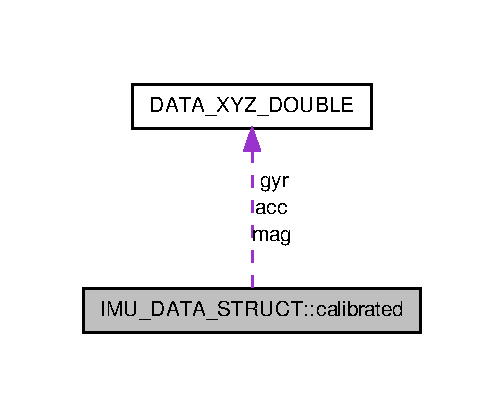
\includegraphics[width=242pt]{structIMU__DATA__STRUCT_1_1calibrated__coll__graph}
\end{center}
\end{figure}
\subsection*{Data Fields}
\begin{DoxyCompactItemize}
\item 
\hyperlink{structDATA__XYZ__DOUBLE}{D\-A\-T\-A\-\_\-\-X\-Y\-Z\-\_\-\-D\-O\-U\-B\-L\-E} \hyperlink{structIMU__DATA__STRUCT_1_1calibrated_a281a7fdb40a05ed97388f18b9bb90c81}{acc}
\item 
\hyperlink{structDATA__XYZ__DOUBLE}{D\-A\-T\-A\-\_\-\-X\-Y\-Z\-\_\-\-D\-O\-U\-B\-L\-E} \hyperlink{structIMU__DATA__STRUCT_1_1calibrated_a8a54aded6ce608f1b7d2b4a0c52c248b}{gyr}
\item 
\hyperlink{structDATA__XYZ__DOUBLE}{D\-A\-T\-A\-\_\-\-X\-Y\-Z\-\_\-\-D\-O\-U\-B\-L\-E} \hyperlink{structIMU__DATA__STRUCT_1_1calibrated_a2fde6c6759e0fda17e272c32096cb9ec}{mag}
\end{DoxyCompactItemize}


\subsection{Detailed Description}


Definition at line 94 of file communication.\-h.



\subsection{Field Documentation}
\hypertarget{structIMU__DATA__STRUCT_1_1calibrated_a281a7fdb40a05ed97388f18b9bb90c81}{\index{I\-M\-U\-\_\-\-D\-A\-T\-A\-\_\-\-S\-T\-R\-U\-C\-T\-::calibrated@{I\-M\-U\-\_\-\-D\-A\-T\-A\-\_\-\-S\-T\-R\-U\-C\-T\-::calibrated}!acc@{acc}}
\index{acc@{acc}!IMU_DATA_STRUCT::calibrated@{I\-M\-U\-\_\-\-D\-A\-T\-A\-\_\-\-S\-T\-R\-U\-C\-T\-::calibrated}}
\subsubsection[{acc}]{\setlength{\rightskip}{0pt plus 5cm}{\bf D\-A\-T\-A\-\_\-\-X\-Y\-Z\-\_\-\-D\-O\-U\-B\-L\-E} I\-M\-U\-\_\-\-D\-A\-T\-A\-\_\-\-S\-T\-R\-U\-C\-T\-::calibrated\-::acc}}\label{structIMU__DATA__STRUCT_1_1calibrated_a281a7fdb40a05ed97388f18b9bb90c81}


Definition at line 95 of file communication.\-h.



Referenced by calibrate\-\_\-imu(), datalogger\-\_\-update(), ui\-\_\-imu\-\_\-data(), and ui\-\_\-overview\-\_\-data().

\hypertarget{structIMU__DATA__STRUCT_1_1calibrated_a8a54aded6ce608f1b7d2b4a0c52c248b}{\index{I\-M\-U\-\_\-\-D\-A\-T\-A\-\_\-\-S\-T\-R\-U\-C\-T\-::calibrated@{I\-M\-U\-\_\-\-D\-A\-T\-A\-\_\-\-S\-T\-R\-U\-C\-T\-::calibrated}!gyr@{gyr}}
\index{gyr@{gyr}!IMU_DATA_STRUCT::calibrated@{I\-M\-U\-\_\-\-D\-A\-T\-A\-\_\-\-S\-T\-R\-U\-C\-T\-::calibrated}}
\subsubsection[{gyr}]{\setlength{\rightskip}{0pt plus 5cm}{\bf D\-A\-T\-A\-\_\-\-X\-Y\-Z\-\_\-\-D\-O\-U\-B\-L\-E} I\-M\-U\-\_\-\-D\-A\-T\-A\-\_\-\-S\-T\-R\-U\-C\-T\-::calibrated\-::gyr}}\label{structIMU__DATA__STRUCT_1_1calibrated_a8a54aded6ce608f1b7d2b4a0c52c248b}


Definition at line 96 of file communication.\-h.



Referenced by calibrate\-\_\-imu(), datalogger\-\_\-update(), ui\-\_\-imu\-\_\-data(), and ui\-\_\-overview\-\_\-data().

\hypertarget{structIMU__DATA__STRUCT_1_1calibrated_a2fde6c6759e0fda17e272c32096cb9ec}{\index{I\-M\-U\-\_\-\-D\-A\-T\-A\-\_\-\-S\-T\-R\-U\-C\-T\-::calibrated@{I\-M\-U\-\_\-\-D\-A\-T\-A\-\_\-\-S\-T\-R\-U\-C\-T\-::calibrated}!mag@{mag}}
\index{mag@{mag}!IMU_DATA_STRUCT::calibrated@{I\-M\-U\-\_\-\-D\-A\-T\-A\-\_\-\-S\-T\-R\-U\-C\-T\-::calibrated}}
\subsubsection[{mag}]{\setlength{\rightskip}{0pt plus 5cm}{\bf D\-A\-T\-A\-\_\-\-X\-Y\-Z\-\_\-\-D\-O\-U\-B\-L\-E} I\-M\-U\-\_\-\-D\-A\-T\-A\-\_\-\-S\-T\-R\-U\-C\-T\-::calibrated\-::mag}}\label{structIMU__DATA__STRUCT_1_1calibrated_a2fde6c6759e0fda17e272c32096cb9ec}


Definition at line 97 of file communication.\-h.



Referenced by calibrate\-\_\-imu(), datalogger\-\_\-update(), ui\-\_\-imu\-\_\-data(), and ui\-\_\-overview\-\_\-data().



The documentation for this struct was generated from the following file\-:\begin{DoxyCompactItemize}
\item 
communication/\hyperlink{communication_2communication_8h}{communication.\-h}\end{DoxyCompactItemize}

\hypertarget{structDATA__XYZ}{
\section{DATA\_\-XYZ Struct Reference}
\label{structDATA__XYZ}\index{DATA\_\-XYZ@{DATA\_\-XYZ}}
}


A structure to represent a 3d Vector.  




{\ttfamily \#include \char`\"{}communication.h\char`\"{}}

\subsection*{Data Fields}
\begin{DoxyCompactItemize}
\item 
short int \hyperlink{structDATA__XYZ_a54c1596e9f9969fd9c21e8458024ecfb}{x}
\item 
short int \hyperlink{structDATA__XYZ_a94bbb1c889bf53eb6a5fffa2b39322cf}{y}
\item 
short int \hyperlink{structDATA__XYZ_a69e89ab0ec6e5d72fc5d54f62cc07fb5}{z}
\end{DoxyCompactItemize}


\subsection{Detailed Description}
A structure to represent a 3d Vector. 

Definition at line 75 of file communication.h.



\subsection{Field Documentation}
\hypertarget{structDATA__XYZ_a54c1596e9f9969fd9c21e8458024ecfb}{
\index{DATA\_\-XYZ@{DATA\_\-XYZ}!x@{x}}
\index{x@{x}!DATA_XYZ@{DATA\_\-XYZ}}
\subsubsection[{x}]{\setlength{\rightskip}{0pt plus 5cm}short int {\bf DATA\_\-XYZ::x}}}
\label{structDATA__XYZ_a54c1596e9f9969fd9c21e8458024ecfb}


Definition at line 76 of file communication.h.



Referenced by calibrate\_\-imu(), control\_\-main(), datalogger\_\-update(), periodic\_\-task\_\-2(), read\_\-all\_\-data(), ui\_\-eff\_\-data(), ui\_\-imu\_\-data(), and ui\_\-overview\_\-data().

\hypertarget{structDATA__XYZ_a94bbb1c889bf53eb6a5fffa2b39322cf}{
\index{DATA\_\-XYZ@{DATA\_\-XYZ}!y@{y}}
\index{y@{y}!DATA_XYZ@{DATA\_\-XYZ}}
\subsubsection[{y}]{\setlength{\rightskip}{0pt plus 5cm}short int {\bf DATA\_\-XYZ::y}}}
\label{structDATA__XYZ_a94bbb1c889bf53eb6a5fffa2b39322cf}


Definition at line 77 of file communication.h.



Referenced by calibrate\_\-imu(), datalogger\_\-update(), periodic\_\-task\_\-2(), read\_\-all\_\-data(), ui\_\-eff\_\-data(), ui\_\-imu\_\-data(), and ui\_\-overview\_\-data().

\hypertarget{structDATA__XYZ_a69e89ab0ec6e5d72fc5d54f62cc07fb5}{
\index{DATA\_\-XYZ@{DATA\_\-XYZ}!z@{z}}
\index{z@{z}!DATA_XYZ@{DATA\_\-XYZ}}
\subsubsection[{z}]{\setlength{\rightskip}{0pt plus 5cm}short int {\bf DATA\_\-XYZ::z}}}
\label{structDATA__XYZ_a69e89ab0ec6e5d72fc5d54f62cc07fb5}


Definition at line 78 of file communication.h.



Referenced by calibrate\_\-imu(), control\_\-main(), datalogger\_\-update(), periodic\_\-task\_\-2(), read\_\-all\_\-data(), ui\_\-eff\_\-data(), ui\_\-imu\_\-data(), and ui\_\-overview\_\-data().



The documentation for this struct was generated from the following file:\begin{DoxyCompactItemize}
\item 
communication/\hyperlink{communication_8h}{communication.h}\end{DoxyCompactItemize}

\hypertarget{structDATA__XYZ__DOUBLE}{
\section{DATA\_\-XYZ\_\-DOUBLE Struct Reference}
\label{structDATA__XYZ__DOUBLE}\index{DATA\_\-XYZ\_\-DOUBLE@{DATA\_\-XYZ\_\-DOUBLE}}
}


Vector definition on double.  




{\ttfamily \#include \char`\"{}communication.h\char`\"{}}

\subsection*{Data Fields}
\begin{DoxyCompactItemize}
\item 
double \hyperlink{structDATA__XYZ__DOUBLE_a22868cc99a423900e7b82d015a5eb91f}{x}
\item 
double \hyperlink{structDATA__XYZ__DOUBLE_a198a27b5df3b5b0bf461b0e481e22a82}{y}
\item 
double \hyperlink{structDATA__XYZ__DOUBLE_a9556e8868c223ff3e28756ea18a284c0}{z}
\end{DoxyCompactItemize}


\subsection{Detailed Description}
Vector definition on double. 

Definition at line 84 of file communication.h.



\subsection{Field Documentation}
\hypertarget{structDATA__XYZ__DOUBLE_a22868cc99a423900e7b82d015a5eb91f}{
\index{DATA\_\-XYZ\_\-DOUBLE@{DATA\_\-XYZ\_\-DOUBLE}!x@{x}}
\index{x@{x}!DATA_XYZ_DOUBLE@{DATA\_\-XYZ\_\-DOUBLE}}
\subsubsection[{x}]{\setlength{\rightskip}{0pt plus 5cm}double {\bf DATA\_\-XYZ\_\-DOUBLE::x}}}
\label{structDATA__XYZ__DOUBLE_a22868cc99a423900e7b82d015a5eb91f}


Definition at line 85 of file communication.h.



Referenced by calibrate\_\-imu(), datalogger\_\-update(), ui\_\-imu\_\-data(), and ui\_\-overview\_\-data().

\hypertarget{structDATA__XYZ__DOUBLE_a198a27b5df3b5b0bf461b0e481e22a82}{
\index{DATA\_\-XYZ\_\-DOUBLE@{DATA\_\-XYZ\_\-DOUBLE}!y@{y}}
\index{y@{y}!DATA_XYZ_DOUBLE@{DATA\_\-XYZ\_\-DOUBLE}}
\subsubsection[{y}]{\setlength{\rightskip}{0pt plus 5cm}double {\bf DATA\_\-XYZ\_\-DOUBLE::y}}}
\label{structDATA__XYZ__DOUBLE_a198a27b5df3b5b0bf461b0e481e22a82}


Definition at line 86 of file communication.h.



Referenced by calibrate\_\-imu(), datalogger\_\-update(), ui\_\-imu\_\-data(), and ui\_\-overview\_\-data().

\hypertarget{structDATA__XYZ__DOUBLE_a9556e8868c223ff3e28756ea18a284c0}{
\index{DATA\_\-XYZ\_\-DOUBLE@{DATA\_\-XYZ\_\-DOUBLE}!z@{z}}
\index{z@{z}!DATA_XYZ_DOUBLE@{DATA\_\-XYZ\_\-DOUBLE}}
\subsubsection[{z}]{\setlength{\rightskip}{0pt plus 5cm}double {\bf DATA\_\-XYZ\_\-DOUBLE::z}}}
\label{structDATA__XYZ__DOUBLE_a9556e8868c223ff3e28756ea18a284c0}


Definition at line 87 of file communication.h.



Referenced by calibrate\_\-imu(), datalogger\_\-update(), ui\_\-imu\_\-data(), and ui\_\-overview\_\-data().



The documentation for this struct was generated from the following file:\begin{DoxyCompactItemize}
\item 
communication/\hyperlink{communication_8h}{communication.h}\end{DoxyCompactItemize}

\hypertarget{structEFF__DATA__STRUCT}{
\section{EFF\_\-DATA\_\-STRUCT Struct Reference}
\label{structEFF__DATA__STRUCT}\index{EFF\_\-DATA\_\-STRUCT@{EFF\_\-DATA\_\-STRUCT}}
}


{\ttfamily \#include \char`\"{}communication.h\char`\"{}}



Collaboration diagram for EFF\_\-DATA\_\-STRUCT:\subsection*{Data Fields}
\begin{DoxyCompactItemize}
\item 
\hyperlink{structDATA__XYZ}{DATA\_\-XYZ} \hyperlink{structEFF__DATA__STRUCT_abe8952947b54bf9c247f3429ee3aeb44}{F}
\item 
\hyperlink{structDATA__XYZ}{DATA\_\-XYZ} \hyperlink{structEFF__DATA__STRUCT_aaf6e03b6e600295e0f5c706fc869e9d1}{M}
\item 
uint8\_\-t \hyperlink{structEFF__DATA__STRUCT_aa42ebc512dd79fa6ebf998162a149446}{new\_\-data}
\end{DoxyCompactItemize}


\subsection{Detailed Description}


Definition at line 112 of file communication.h.



\subsection{Field Documentation}
\hypertarget{structEFF__DATA__STRUCT_abe8952947b54bf9c247f3429ee3aeb44}{
\index{EFF\_\-DATA\_\-STRUCT@{EFF\_\-DATA\_\-STRUCT}!F@{F}}
\index{F@{F}!EFF_DATA_STRUCT@{EFF\_\-DATA\_\-STRUCT}}
\subsubsection[{F}]{\setlength{\rightskip}{0pt plus 5cm}{\bf DATA\_\-XYZ} {\bf EFF\_\-DATA\_\-STRUCT::F}}}
\label{structEFF__DATA__STRUCT_abe8952947b54bf9c247f3429ee3aeb44}


Definition at line 113 of file communication.h.



Referenced by datalogger\_\-update(), read\_\-all\_\-data(), and ui\_\-eff\_\-data().

\hypertarget{structEFF__DATA__STRUCT_aaf6e03b6e600295e0f5c706fc869e9d1}{
\index{EFF\_\-DATA\_\-STRUCT@{EFF\_\-DATA\_\-STRUCT}!M@{M}}
\index{M@{M}!EFF_DATA_STRUCT@{EFF\_\-DATA\_\-STRUCT}}
\subsubsection[{M}]{\setlength{\rightskip}{0pt plus 5cm}{\bf DATA\_\-XYZ} {\bf EFF\_\-DATA\_\-STRUCT::M}}}
\label{structEFF__DATA__STRUCT_aaf6e03b6e600295e0f5c706fc869e9d1}


Definition at line 114 of file communication.h.



Referenced by ui\_\-eff\_\-data().

\hypertarget{structEFF__DATA__STRUCT_aa42ebc512dd79fa6ebf998162a149446}{
\index{EFF\_\-DATA\_\-STRUCT@{EFF\_\-DATA\_\-STRUCT}!new\_\-data@{new\_\-data}}
\index{new\_\-data@{new\_\-data}!EFF_DATA_STRUCT@{EFF\_\-DATA\_\-STRUCT}}
\subsubsection[{new\_\-data}]{\setlength{\rightskip}{0pt plus 5cm}uint8\_\-t {\bf EFF\_\-DATA\_\-STRUCT::new\_\-data}}}
\label{structEFF__DATA__STRUCT_aa42ebc512dd79fa6ebf998162a149446}


Definition at line 115 of file communication.h.



Referenced by datalogger\_\-update(), and read\_\-all\_\-data().



The documentation for this struct was generated from the following file:\begin{DoxyCompactItemize}
\item 
communication/\hyperlink{communication_8h}{communication.h}\end{DoxyCompactItemize}

\hypertarget{structENC__DATA__STRUCT}{\section{E\-N\-C\-\_\-\-D\-A\-T\-A\-\_\-\-S\-T\-R\-U\-C\-T Struct Reference}
\label{structENC__DATA__STRUCT}\index{E\-N\-C\-\_\-\-D\-A\-T\-A\-\_\-\-S\-T\-R\-U\-C\-T@{E\-N\-C\-\_\-\-D\-A\-T\-A\-\_\-\-S\-T\-R\-U\-C\-T}}
}


{\ttfamily \#include \char`\"{}encoder\-\_\-functions.\-h\char`\"{}}



Collaboration diagram for E\-N\-C\-\_\-\-D\-A\-T\-A\-\_\-\-S\-T\-R\-U\-C\-T\-:
\nopagebreak
\begin{figure}[H]
\begin{center}
\leavevmode
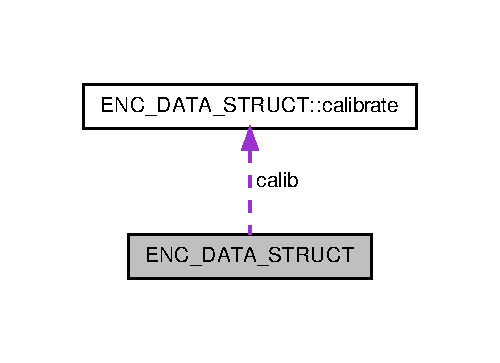
\includegraphics[width=240pt]{structENC__DATA__STRUCT__coll__graph}
\end{center}
\end{figure}
\subsection*{Data Structures}
\begin{DoxyCompactItemize}
\item 
struct \hyperlink{structENC__DATA__STRUCT_1_1calibrate}{calibrate}
\end{DoxyCompactItemize}
\subsection*{Data Fields}
\begin{DoxyCompactItemize}
\item 
int \hyperlink{structENC__DATA__STRUCT_a93b8e925392a12a8874bf59f2a1cd76a}{spi\-\_\-dev}
\item 
unsigned short int \hyperlink{structENC__DATA__STRUCT_ac3a53ed44ecaf87285518a091e1d2c24}{position}
\item 
struct \hyperlink{structENC__DATA__STRUCT_1_1calibrate}{E\-N\-C\-\_\-\-D\-A\-T\-A\-\_\-\-S\-T\-R\-U\-C\-T\-::calibrate} \hyperlink{structENC__DATA__STRUCT_af227e5bbb714b830cc570432bda0a468}{calib}
\item 
int \hyperlink{structENC__DATA__STRUCT_adbfb6e5764f0e3c42f4e212deb5d1f21}{new\-\_\-data}
\end{DoxyCompactItemize}


\subsection{Detailed Description}


Definition at line 45 of file encoder\-\_\-functions.\-h.



\subsection{Field Documentation}
\hypertarget{structENC__DATA__STRUCT_af227e5bbb714b830cc570432bda0a468}{\index{E\-N\-C\-\_\-\-D\-A\-T\-A\-\_\-\-S\-T\-R\-U\-C\-T@{E\-N\-C\-\_\-\-D\-A\-T\-A\-\_\-\-S\-T\-R\-U\-C\-T}!calib@{calib}}
\index{calib@{calib}!ENC_DATA_STRUCT@{E\-N\-C\-\_\-\-D\-A\-T\-A\-\_\-\-S\-T\-R\-U\-C\-T}}
\subsubsection[{calib}]{\setlength{\rightskip}{0pt plus 5cm}struct {\bf E\-N\-C\-\_\-\-D\-A\-T\-A\-\_\-\-S\-T\-R\-U\-C\-T\-::calibrate} E\-N\-C\-\_\-\-D\-A\-T\-A\-\_\-\-S\-T\-R\-U\-C\-T\-::calib}}\label{structENC__DATA__STRUCT_af227e5bbb714b830cc570432bda0a468}


Referenced by calibrate\-\_\-enc(), read\-\_\-all\-\_\-data(), ui\-\_\-enc\-\_\-data(), and ui\-\_\-overview\-\_\-data().

\hypertarget{structENC__DATA__STRUCT_adbfb6e5764f0e3c42f4e212deb5d1f21}{\index{E\-N\-C\-\_\-\-D\-A\-T\-A\-\_\-\-S\-T\-R\-U\-C\-T@{E\-N\-C\-\_\-\-D\-A\-T\-A\-\_\-\-S\-T\-R\-U\-C\-T}!new\-\_\-data@{new\-\_\-data}}
\index{new\-\_\-data@{new\-\_\-data}!ENC_DATA_STRUCT@{E\-N\-C\-\_\-\-D\-A\-T\-A\-\_\-\-S\-T\-R\-U\-C\-T}}
\subsubsection[{new\-\_\-data}]{\setlength{\rightskip}{0pt plus 5cm}int E\-N\-C\-\_\-\-D\-A\-T\-A\-\_\-\-S\-T\-R\-U\-C\-T\-::new\-\_\-data}}\label{structENC__DATA__STRUCT_adbfb6e5764f0e3c42f4e212deb5d1f21}


Definition at line 51 of file encoder\-\_\-functions.\-h.



Referenced by read\-\_\-all\-\_\-data().

\hypertarget{structENC__DATA__STRUCT_ac3a53ed44ecaf87285518a091e1d2c24}{\index{E\-N\-C\-\_\-\-D\-A\-T\-A\-\_\-\-S\-T\-R\-U\-C\-T@{E\-N\-C\-\_\-\-D\-A\-T\-A\-\_\-\-S\-T\-R\-U\-C\-T}!position@{position}}
\index{position@{position}!ENC_DATA_STRUCT@{E\-N\-C\-\_\-\-D\-A\-T\-A\-\_\-\-S\-T\-R\-U\-C\-T}}
\subsubsection[{position}]{\setlength{\rightskip}{0pt plus 5cm}unsigned short int E\-N\-C\-\_\-\-D\-A\-T\-A\-\_\-\-S\-T\-R\-U\-C\-T\-::position}}\label{structENC__DATA__STRUCT_ac3a53ed44ecaf87285518a091e1d2c24}


Definition at line 47 of file encoder\-\_\-functions.\-h.



Referenced by calibrate\-\_\-enc(), read\-\_\-all\-\_\-data(), ui\-\_\-enc\-\_\-data(), and ui\-\_\-overview\-\_\-data().

\hypertarget{structENC__DATA__STRUCT_a93b8e925392a12a8874bf59f2a1cd76a}{\index{E\-N\-C\-\_\-\-D\-A\-T\-A\-\_\-\-S\-T\-R\-U\-C\-T@{E\-N\-C\-\_\-\-D\-A\-T\-A\-\_\-\-S\-T\-R\-U\-C\-T}!spi\-\_\-dev@{spi\-\_\-dev}}
\index{spi\-\_\-dev@{spi\-\_\-dev}!ENC_DATA_STRUCT@{E\-N\-C\-\_\-\-D\-A\-T\-A\-\_\-\-S\-T\-R\-U\-C\-T}}
\subsubsection[{spi\-\_\-dev}]{\setlength{\rightskip}{0pt plus 5cm}int E\-N\-C\-\_\-\-D\-A\-T\-A\-\_\-\-S\-T\-R\-U\-C\-T\-::spi\-\_\-dev}}\label{structENC__DATA__STRUCT_a93b8e925392a12a8874bf59f2a1cd76a}


Definition at line 46 of file encoder\-\_\-functions.\-h.



Referenced by read\-\_\-all\-\_\-data().



The documentation for this struct was generated from the following file\-:\begin{DoxyCompactItemize}
\item 
communication/\hyperlink{encoder__functions_8h}{encoder\-\_\-functions.\-h}\end{DoxyCompactItemize}

\hypertarget{structGDATALOGGER}{\section{G\-D\-A\-T\-A\-L\-O\-G\-G\-E\-R Struct Reference}
\label{structGDATALOGGER}\index{G\-D\-A\-T\-A\-L\-O\-G\-G\-E\-R@{G\-D\-A\-T\-A\-L\-O\-G\-G\-E\-R}}
}


{\ttfamily \#include \char`\"{}gdatalogger.\-h\char`\"{}}



Collaboration diagram for G\-D\-A\-T\-A\-L\-O\-G\-G\-E\-R\-:
\nopagebreak
\begin{figure}[H]
\begin{center}
\leavevmode
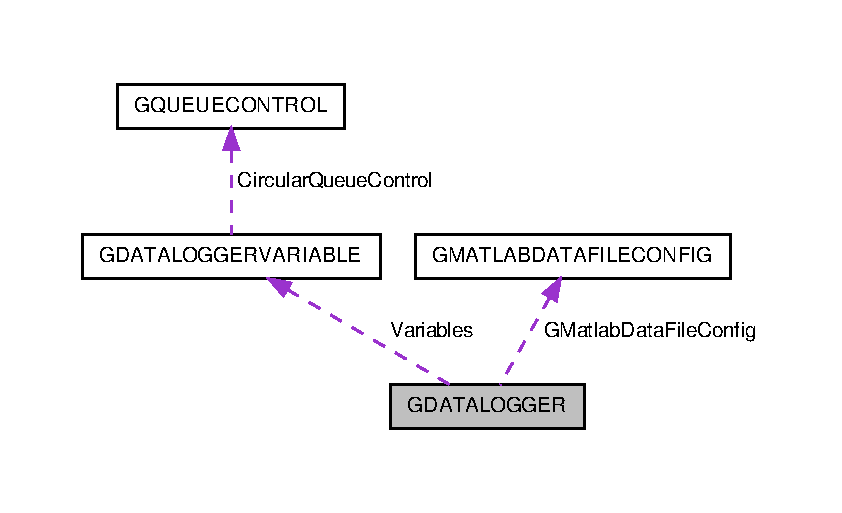
\includegraphics[width=350pt]{structGDATALOGGER__coll__graph}
\end{center}
\end{figure}
\subsection*{Data Fields}
\begin{DoxyCompactItemize}
\item 
\hyperlink{structGDATALOGGERVARIABLE}{G\-D\-A\-T\-A\-L\-O\-G\-G\-E\-R\-V\-A\-R\-I\-A\-B\-L\-E} \hyperlink{structGDATALOGGER_a6af9584d8665205b950cb2dcc5f90a94}{Variables} \mbox{[}\hyperlink{gdatalogger_8h_a2ddc529b6734b7a9222a5fbd1305581e}{G\-D\-A\-T\-A\-L\-O\-G\-G\-E\-R\-\_\-\-M\-A\-X\-V\-A\-R\-I\-A\-B\-L\-E\-S}\mbox{]}
\item 
int \hyperlink{structGDATALOGGER_a2ac727ee6c50f7e04030cbe531158f08}{m\-\_\-\-Number\-Of\-Variables}
\item 
\hyperlink{structGMATLABDATAFILECONFIG}{G\-M\-A\-T\-L\-A\-B\-D\-A\-T\-A\-F\-I\-L\-E\-C\-O\-N\-F\-I\-G} \hyperlink{structGDATALOGGER_a062fd3836dbd0b1bec129ab372bff04a}{G\-Matlab\-Data\-File\-Config}
\end{DoxyCompactItemize}


\subsection{Detailed Description}


Definition at line 26 of file gdatalogger.\-h.



\subsection{Field Documentation}
\hypertarget{structGDATALOGGER_a062fd3836dbd0b1bec129ab372bff04a}{\index{G\-D\-A\-T\-A\-L\-O\-G\-G\-E\-R@{G\-D\-A\-T\-A\-L\-O\-G\-G\-E\-R}!G\-Matlab\-Data\-File\-Config@{G\-Matlab\-Data\-File\-Config}}
\index{G\-Matlab\-Data\-File\-Config@{G\-Matlab\-Data\-File\-Config}!GDATALOGGER@{G\-D\-A\-T\-A\-L\-O\-G\-G\-E\-R}}
\subsubsection[{G\-Matlab\-Data\-File\-Config}]{\setlength{\rightskip}{0pt plus 5cm}{\bf G\-M\-A\-T\-L\-A\-B\-D\-A\-T\-A\-F\-I\-L\-E\-C\-O\-N\-F\-I\-G} G\-D\-A\-T\-A\-L\-O\-G\-G\-E\-R\-::\-G\-Matlab\-Data\-File\-Config}}\label{structGDATALOGGER_a062fd3836dbd0b1bec129ab372bff04a}


Definition at line 29 of file gdatalogger.\-h.



Referenced by g\-Data\-Logger\-\_\-\-Close(), g\-Data\-Logger\-\_\-\-Init(), and g\-Data\-Logger\-\_\-\-Matfile\-Update().

\hypertarget{structGDATALOGGER_a2ac727ee6c50f7e04030cbe531158f08}{\index{G\-D\-A\-T\-A\-L\-O\-G\-G\-E\-R@{G\-D\-A\-T\-A\-L\-O\-G\-G\-E\-R}!m\-\_\-\-Number\-Of\-Variables@{m\-\_\-\-Number\-Of\-Variables}}
\index{m\-\_\-\-Number\-Of\-Variables@{m\-\_\-\-Number\-Of\-Variables}!GDATALOGGER@{G\-D\-A\-T\-A\-L\-O\-G\-G\-E\-R}}
\subsubsection[{m\-\_\-\-Number\-Of\-Variables}]{\setlength{\rightskip}{0pt plus 5cm}int G\-D\-A\-T\-A\-L\-O\-G\-G\-E\-R\-::m\-\_\-\-Number\-Of\-Variables}}\label{structGDATALOGGER_a2ac727ee6c50f7e04030cbe531158f08}


Definition at line 28 of file gdatalogger.\-h.



Referenced by g\-Data\-Logger\-\_\-\-Close(), g\-Data\-Logger\-\_\-\-Declare\-Variable(), g\-Data\-Logger\-\_\-\-Init(), g\-Data\-Logger\-\_\-\-Insert\-Variable(), g\-Data\-Logger\-\_\-\-I\-P\-C\-Update(), and g\-Data\-Logger\-\_\-\-Matfile\-Update().

\hypertarget{structGDATALOGGER_a6af9584d8665205b950cb2dcc5f90a94}{\index{G\-D\-A\-T\-A\-L\-O\-G\-G\-E\-R@{G\-D\-A\-T\-A\-L\-O\-G\-G\-E\-R}!Variables@{Variables}}
\index{Variables@{Variables}!GDATALOGGER@{G\-D\-A\-T\-A\-L\-O\-G\-G\-E\-R}}
\subsubsection[{Variables}]{\setlength{\rightskip}{0pt plus 5cm}{\bf G\-D\-A\-T\-A\-L\-O\-G\-G\-E\-R\-V\-A\-R\-I\-A\-B\-L\-E} G\-D\-A\-T\-A\-L\-O\-G\-G\-E\-R\-::\-Variables\mbox{[}{\bf G\-D\-A\-T\-A\-L\-O\-G\-G\-E\-R\-\_\-\-M\-A\-X\-V\-A\-R\-I\-A\-B\-L\-E\-S}\mbox{]}}}\label{structGDATALOGGER_a6af9584d8665205b950cb2dcc5f90a94}


Definition at line 27 of file gdatalogger.\-h.



Referenced by g\-Data\-Logger\-\_\-\-Close(), g\-Data\-Logger\-\_\-\-Declare\-Variable(), g\-Data\-Logger\-\_\-\-Init(), g\-Data\-Logger\-\_\-\-Insert\-Variable(), g\-Data\-Logger\-\_\-\-I\-P\-C\-Update(), and g\-Data\-Logger\-\_\-\-Matfile\-Update().



The documentation for this struct was generated from the following file\-:\begin{DoxyCompactItemize}
\item 
gdatalogger/\hyperlink{gdatalogger_8h}{gdatalogger.\-h}\end{DoxyCompactItemize}

\hypertarget{structGDATALOGGERIPC__SHM}{
\section{GDATALOGGERIPC\_\-SHM Struct Reference}
\label{structGDATALOGGERIPC__SHM}\index{GDATALOGGERIPC\_\-SHM@{GDATALOGGERIPC\_\-SHM}}
}


{\ttfamily \#include \char`\"{}gdatalogger.h\char`\"{}}

\subsection*{Data Fields}
\begin{DoxyCompactItemize}
\item 
char \hyperlink{structGDATALOGGERIPC__SHM_afb130e15f688a18e52e2037f4bb17e89}{VariableName} \mbox{[}100\mbox{]}
\item 
char \hyperlink{structGDATALOGGERIPC__SHM_a8efd7b2ed8ff087f9694cb47a8c25a13}{VariableUnit} \mbox{[}50\mbox{]}
\item 
double \hyperlink{structGDATALOGGERIPC__SHM_ac495752de142e6697c08f713505ed55c}{QueueData} \mbox{[}GDATALOGGER\_\-IPC\_\-MAXQUEUESIZE\mbox{]}
\item 
int \hyperlink{structGDATALOGGERIPC__SHM_a7d392777d231e1b0cece66cb51b0945b}{QueueSize}
\item 
int \hyperlink{structGDATALOGGERIPC__SHM_a346eca077a97246740a6ed4f7c08833c}{Flag}
\end{DoxyCompactItemize}


\subsection{Detailed Description}


Definition at line 45 of file gdatalogger.h.



\subsection{Field Documentation}
\hypertarget{structGDATALOGGERIPC__SHM_a346eca077a97246740a6ed4f7c08833c}{
\index{GDATALOGGERIPC\_\-SHM@{GDATALOGGERIPC\_\-SHM}!Flag@{Flag}}
\index{Flag@{Flag}!GDATALOGGERIPC_SHM@{GDATALOGGERIPC\_\-SHM}}
\subsubsection[{Flag}]{\setlength{\rightskip}{0pt plus 5cm}int {\bf GDATALOGGERIPC\_\-SHM::Flag}}}
\label{structGDATALOGGERIPC__SHM_a346eca077a97246740a6ed4f7c08833c}


Definition at line 50 of file gdatalogger.h.



Referenced by gDataLogger\_\-Init(), gDataLogger\_\-IPC\_\-RetrieveVariable(), and gDataLogger\_\-IPCUpdate().

\hypertarget{structGDATALOGGERIPC__SHM_ac495752de142e6697c08f713505ed55c}{
\index{GDATALOGGERIPC\_\-SHM@{GDATALOGGERIPC\_\-SHM}!QueueData@{QueueData}}
\index{QueueData@{QueueData}!GDATALOGGERIPC_SHM@{GDATALOGGERIPC\_\-SHM}}
\subsubsection[{QueueData}]{\setlength{\rightskip}{0pt plus 5cm}double {\bf GDATALOGGERIPC\_\-SHM::QueueData}\mbox{[}GDATALOGGER\_\-IPC\_\-MAXQUEUESIZE\mbox{]}}}
\label{structGDATALOGGERIPC__SHM_ac495752de142e6697c08f713505ed55c}


Definition at line 48 of file gdatalogger.h.



Referenced by gDataLogger\_\-IPC\_\-RetrieveVariable(), and gDataLogger\_\-IPCUpdate().

\hypertarget{structGDATALOGGERIPC__SHM_a7d392777d231e1b0cece66cb51b0945b}{
\index{GDATALOGGERIPC\_\-SHM@{GDATALOGGERIPC\_\-SHM}!QueueSize@{QueueSize}}
\index{QueueSize@{QueueSize}!GDATALOGGERIPC_SHM@{GDATALOGGERIPC\_\-SHM}}
\subsubsection[{QueueSize}]{\setlength{\rightskip}{0pt plus 5cm}int {\bf GDATALOGGERIPC\_\-SHM::QueueSize}}}
\label{structGDATALOGGERIPC__SHM_a7d392777d231e1b0cece66cb51b0945b}


Definition at line 49 of file gdatalogger.h.



Referenced by gDataLogger\_\-IPC\_\-RetrieveVariable(), and gDataLogger\_\-IPCUpdate().

\hypertarget{structGDATALOGGERIPC__SHM_afb130e15f688a18e52e2037f4bb17e89}{
\index{GDATALOGGERIPC\_\-SHM@{GDATALOGGERIPC\_\-SHM}!VariableName@{VariableName}}
\index{VariableName@{VariableName}!GDATALOGGERIPC_SHM@{GDATALOGGERIPC\_\-SHM}}
\subsubsection[{VariableName}]{\setlength{\rightskip}{0pt plus 5cm}char {\bf GDATALOGGERIPC\_\-SHM::VariableName}\mbox{[}100\mbox{]}}}
\label{structGDATALOGGERIPC__SHM_afb130e15f688a18e52e2037f4bb17e89}


Definition at line 46 of file gdatalogger.h.



Referenced by gDataLogger\_\-IPC\_\-RetrieveVariable(), and gDataLogger\_\-IPCUpdate().

\hypertarget{structGDATALOGGERIPC__SHM_a8efd7b2ed8ff087f9694cb47a8c25a13}{
\index{GDATALOGGERIPC\_\-SHM@{GDATALOGGERIPC\_\-SHM}!VariableUnit@{VariableUnit}}
\index{VariableUnit@{VariableUnit}!GDATALOGGERIPC_SHM@{GDATALOGGERIPC\_\-SHM}}
\subsubsection[{VariableUnit}]{\setlength{\rightskip}{0pt plus 5cm}char {\bf GDATALOGGERIPC\_\-SHM::VariableUnit}\mbox{[}50\mbox{]}}}
\label{structGDATALOGGERIPC__SHM_a8efd7b2ed8ff087f9694cb47a8c25a13}


Definition at line 47 of file gdatalogger.h.



Referenced by gDataLogger\_\-IPC\_\-RetrieveVariable(), and gDataLogger\_\-IPCUpdate().



The documentation for this struct was generated from the following file:\begin{DoxyCompactItemize}
\item 
gdatalogger/\hyperlink{gdatalogger_8h}{gdatalogger.h}\end{DoxyCompactItemize}

\hypertarget{structGDATALOGGERVARIABLE}{\section{G\-D\-A\-T\-A\-L\-O\-G\-G\-E\-R\-V\-A\-R\-I\-A\-B\-L\-E Struct Reference}
\label{structGDATALOGGERVARIABLE}\index{G\-D\-A\-T\-A\-L\-O\-G\-G\-E\-R\-V\-A\-R\-I\-A\-B\-L\-E@{G\-D\-A\-T\-A\-L\-O\-G\-G\-E\-R\-V\-A\-R\-I\-A\-B\-L\-E}}
}


{\ttfamily \#include \char`\"{}gdatalogger.\-h\char`\"{}}



Collaboration diagram for G\-D\-A\-T\-A\-L\-O\-G\-G\-E\-R\-V\-A\-R\-I\-A\-B\-L\-E\-:\nopagebreak
\begin{figure}[H]
\begin{center}
\leavevmode
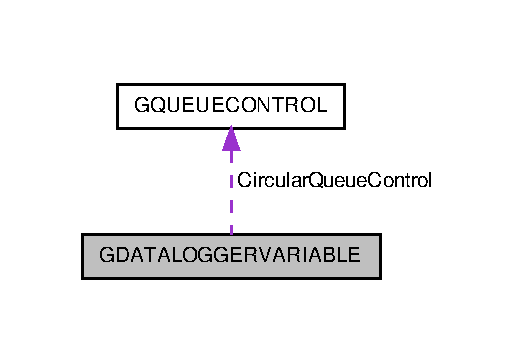
\includegraphics[width=248pt]{structGDATALOGGERVARIABLE__coll__graph}
\end{center}
\end{figure}
\subsection*{Data Fields}
\begin{DoxyCompactItemize}
\item 
char \hyperlink{structGDATALOGGERVARIABLE_a336b7b6cbfc9cdebc7e1ade3de17ac3f}{Variable\-Name} \mbox{[}100\mbox{]}
\item 
char \hyperlink{structGDATALOGGERVARIABLE_a0d42da63f3f904774cbf2ee8d92ee135}{Variable\-Unit} \mbox{[}50\mbox{]}
\item 
long int \hyperlink{structGDATALOGGERVARIABLE_aa1cd5b838d8655734e7d4499b25bf22a}{G\-Matlab\-Data\-File\-Index}
\item 
int \hyperlink{structGDATALOGGERVARIABLE_a68c3eb0f57a786afe9a2658fc42b61d6}{Nr}
\item 
int \hyperlink{structGDATALOGGERVARIABLE_abd1db7599f09e121cd125e665cb9c460}{Nc}
\item 
double $\ast$ \hyperlink{structGDATALOGGERVARIABLE_ae17ad02442f31da9518c99ce13607c8b}{Circular\-Queue}
\item 
\hyperlink{structGQUEUECONTROL}{G\-Q\-U\-E\-U\-E\-C\-O\-N\-T\-R\-O\-L} \hyperlink{structGDATALOGGERVARIABLE_a1a50747d2223f228288b4656470d9bbc}{Circular\-Queue\-Control}
\item 
int \hyperlink{structGDATALOGGERVARIABLE_ad982aef10e8496c2a1c6b9bb1f1dc5c3}{Has\-Been\-Written}
\end{DoxyCompactItemize}


\subsection{Detailed Description}


Definition at line 15 of file gdatalogger.\-h.



\subsection{Field Documentation}
\hypertarget{structGDATALOGGERVARIABLE_ae17ad02442f31da9518c99ce13607c8b}{\index{G\-D\-A\-T\-A\-L\-O\-G\-G\-E\-R\-V\-A\-R\-I\-A\-B\-L\-E@{G\-D\-A\-T\-A\-L\-O\-G\-G\-E\-R\-V\-A\-R\-I\-A\-B\-L\-E}!Circular\-Queue@{Circular\-Queue}}
\index{Circular\-Queue@{Circular\-Queue}!GDATALOGGERVARIABLE@{G\-D\-A\-T\-A\-L\-O\-G\-G\-E\-R\-V\-A\-R\-I\-A\-B\-L\-E}}
\subsubsection[{Circular\-Queue}]{\setlength{\rightskip}{0pt plus 5cm}double$\ast$ G\-D\-A\-T\-A\-L\-O\-G\-G\-E\-R\-V\-A\-R\-I\-A\-B\-L\-E\-::\-Circular\-Queue}}\label{structGDATALOGGERVARIABLE_ae17ad02442f31da9518c99ce13607c8b}


Definition at line 21 of file gdatalogger.\-h.



Referenced by g\-Data\-Logger\-\_\-\-Close(), g\-Data\-Logger\-\_\-\-Declare\-Variable(), g\-Data\-Logger\-\_\-\-Init(), g\-Data\-Logger\-\_\-\-Insert\-Variable(), g\-Data\-Logger\-\_\-\-I\-P\-C\-Update(), and g\-Data\-Logger\-\_\-\-Matfile\-Update().

\hypertarget{structGDATALOGGERVARIABLE_a1a50747d2223f228288b4656470d9bbc}{\index{G\-D\-A\-T\-A\-L\-O\-G\-G\-E\-R\-V\-A\-R\-I\-A\-B\-L\-E@{G\-D\-A\-T\-A\-L\-O\-G\-G\-E\-R\-V\-A\-R\-I\-A\-B\-L\-E}!Circular\-Queue\-Control@{Circular\-Queue\-Control}}
\index{Circular\-Queue\-Control@{Circular\-Queue\-Control}!GDATALOGGERVARIABLE@{G\-D\-A\-T\-A\-L\-O\-G\-G\-E\-R\-V\-A\-R\-I\-A\-B\-L\-E}}
\subsubsection[{Circular\-Queue\-Control}]{\setlength{\rightskip}{0pt plus 5cm}{\bf G\-Q\-U\-E\-U\-E\-C\-O\-N\-T\-R\-O\-L} G\-D\-A\-T\-A\-L\-O\-G\-G\-E\-R\-V\-A\-R\-I\-A\-B\-L\-E\-::\-Circular\-Queue\-Control}}\label{structGDATALOGGERVARIABLE_a1a50747d2223f228288b4656470d9bbc}


Definition at line 22 of file gdatalogger.\-h.



Referenced by g\-Data\-Logger\-\_\-\-Declare\-Variable(), g\-Data\-Logger\-\_\-\-Insert\-Variable(), g\-Data\-Logger\-\_\-\-I\-P\-C\-Update(), and g\-Data\-Logger\-\_\-\-Matfile\-Update().

\hypertarget{structGDATALOGGERVARIABLE_aa1cd5b838d8655734e7d4499b25bf22a}{\index{G\-D\-A\-T\-A\-L\-O\-G\-G\-E\-R\-V\-A\-R\-I\-A\-B\-L\-E@{G\-D\-A\-T\-A\-L\-O\-G\-G\-E\-R\-V\-A\-R\-I\-A\-B\-L\-E}!G\-Matlab\-Data\-File\-Index@{G\-Matlab\-Data\-File\-Index}}
\index{G\-Matlab\-Data\-File\-Index@{G\-Matlab\-Data\-File\-Index}!GDATALOGGERVARIABLE@{G\-D\-A\-T\-A\-L\-O\-G\-G\-E\-R\-V\-A\-R\-I\-A\-B\-L\-E}}
\subsubsection[{G\-Matlab\-Data\-File\-Index}]{\setlength{\rightskip}{0pt plus 5cm}long int G\-D\-A\-T\-A\-L\-O\-G\-G\-E\-R\-V\-A\-R\-I\-A\-B\-L\-E\-::\-G\-Matlab\-Data\-File\-Index}}\label{structGDATALOGGERVARIABLE_aa1cd5b838d8655734e7d4499b25bf22a}


Definition at line 18 of file gdatalogger.\-h.



Referenced by g\-Data\-Logger\-\_\-\-Close(), g\-Data\-Logger\-\_\-\-Declare\-Variable(), g\-Data\-Logger\-\_\-\-Init(), and g\-Data\-Logger\-\_\-\-Matfile\-Update().

\hypertarget{structGDATALOGGERVARIABLE_ad982aef10e8496c2a1c6b9bb1f1dc5c3}{\index{G\-D\-A\-T\-A\-L\-O\-G\-G\-E\-R\-V\-A\-R\-I\-A\-B\-L\-E@{G\-D\-A\-T\-A\-L\-O\-G\-G\-E\-R\-V\-A\-R\-I\-A\-B\-L\-E}!Has\-Been\-Written@{Has\-Been\-Written}}
\index{Has\-Been\-Written@{Has\-Been\-Written}!GDATALOGGERVARIABLE@{G\-D\-A\-T\-A\-L\-O\-G\-G\-E\-R\-V\-A\-R\-I\-A\-B\-L\-E}}
\subsubsection[{Has\-Been\-Written}]{\setlength{\rightskip}{0pt plus 5cm}int G\-D\-A\-T\-A\-L\-O\-G\-G\-E\-R\-V\-A\-R\-I\-A\-B\-L\-E\-::\-Has\-Been\-Written}}\label{structGDATALOGGERVARIABLE_ad982aef10e8496c2a1c6b9bb1f1dc5c3}


Definition at line 23 of file gdatalogger.\-h.



Referenced by g\-Data\-Logger\-\_\-\-Close(), g\-Data\-Logger\-\_\-\-Init(), and g\-Data\-Logger\-\_\-\-Insert\-Variable().

\hypertarget{structGDATALOGGERVARIABLE_abd1db7599f09e121cd125e665cb9c460}{\index{G\-D\-A\-T\-A\-L\-O\-G\-G\-E\-R\-V\-A\-R\-I\-A\-B\-L\-E@{G\-D\-A\-T\-A\-L\-O\-G\-G\-E\-R\-V\-A\-R\-I\-A\-B\-L\-E}!Nc@{Nc}}
\index{Nc@{Nc}!GDATALOGGERVARIABLE@{G\-D\-A\-T\-A\-L\-O\-G\-G\-E\-R\-V\-A\-R\-I\-A\-B\-L\-E}}
\subsubsection[{Nc}]{\setlength{\rightskip}{0pt plus 5cm}int G\-D\-A\-T\-A\-L\-O\-G\-G\-E\-R\-V\-A\-R\-I\-A\-B\-L\-E\-::\-Nc}}\label{structGDATALOGGERVARIABLE_abd1db7599f09e121cd125e665cb9c460}


Definition at line 20 of file gdatalogger.\-h.



Referenced by g\-Data\-Logger\-\_\-\-Close(), g\-Data\-Logger\-\_\-\-Declare\-Variable(), g\-Data\-Logger\-\_\-\-Init(), and g\-Data\-Logger\-\_\-\-Insert\-Variable().

\hypertarget{structGDATALOGGERVARIABLE_a68c3eb0f57a786afe9a2658fc42b61d6}{\index{G\-D\-A\-T\-A\-L\-O\-G\-G\-E\-R\-V\-A\-R\-I\-A\-B\-L\-E@{G\-D\-A\-T\-A\-L\-O\-G\-G\-E\-R\-V\-A\-R\-I\-A\-B\-L\-E}!Nr@{Nr}}
\index{Nr@{Nr}!GDATALOGGERVARIABLE@{G\-D\-A\-T\-A\-L\-O\-G\-G\-E\-R\-V\-A\-R\-I\-A\-B\-L\-E}}
\subsubsection[{Nr}]{\setlength{\rightskip}{0pt plus 5cm}int G\-D\-A\-T\-A\-L\-O\-G\-G\-E\-R\-V\-A\-R\-I\-A\-B\-L\-E\-::\-Nr}}\label{structGDATALOGGERVARIABLE_a68c3eb0f57a786afe9a2658fc42b61d6}


Definition at line 19 of file gdatalogger.\-h.



Referenced by g\-Data\-Logger\-\_\-\-Close(), g\-Data\-Logger\-\_\-\-Declare\-Variable(), g\-Data\-Logger\-\_\-\-Init(), and g\-Data\-Logger\-\_\-\-Insert\-Variable().

\hypertarget{structGDATALOGGERVARIABLE_a336b7b6cbfc9cdebc7e1ade3de17ac3f}{\index{G\-D\-A\-T\-A\-L\-O\-G\-G\-E\-R\-V\-A\-R\-I\-A\-B\-L\-E@{G\-D\-A\-T\-A\-L\-O\-G\-G\-E\-R\-V\-A\-R\-I\-A\-B\-L\-E}!Variable\-Name@{Variable\-Name}}
\index{Variable\-Name@{Variable\-Name}!GDATALOGGERVARIABLE@{G\-D\-A\-T\-A\-L\-O\-G\-G\-E\-R\-V\-A\-R\-I\-A\-B\-L\-E}}
\subsubsection[{Variable\-Name}]{\setlength{\rightskip}{0pt plus 5cm}char G\-D\-A\-T\-A\-L\-O\-G\-G\-E\-R\-V\-A\-R\-I\-A\-B\-L\-E\-::\-Variable\-Name\mbox{[}100\mbox{]}}}\label{structGDATALOGGERVARIABLE_a336b7b6cbfc9cdebc7e1ade3de17ac3f}


Definition at line 16 of file gdatalogger.\-h.



Referenced by g\-Data\-Logger\-\_\-\-Close(), g\-Data\-Logger\-\_\-\-Declare\-Variable(), g\-Data\-Logger\-\_\-\-Init(), g\-Data\-Logger\-\_\-\-Insert\-Variable(), g\-Data\-Logger\-\_\-\-I\-P\-C\-Update(), and g\-Data\-Logger\-\_\-\-Matfile\-Update().

\hypertarget{structGDATALOGGERVARIABLE_a0d42da63f3f904774cbf2ee8d92ee135}{\index{G\-D\-A\-T\-A\-L\-O\-G\-G\-E\-R\-V\-A\-R\-I\-A\-B\-L\-E@{G\-D\-A\-T\-A\-L\-O\-G\-G\-E\-R\-V\-A\-R\-I\-A\-B\-L\-E}!Variable\-Unit@{Variable\-Unit}}
\index{Variable\-Unit@{Variable\-Unit}!GDATALOGGERVARIABLE@{G\-D\-A\-T\-A\-L\-O\-G\-G\-E\-R\-V\-A\-R\-I\-A\-B\-L\-E}}
\subsubsection[{Variable\-Unit}]{\setlength{\rightskip}{0pt plus 5cm}char G\-D\-A\-T\-A\-L\-O\-G\-G\-E\-R\-V\-A\-R\-I\-A\-B\-L\-E\-::\-Variable\-Unit\mbox{[}50\mbox{]}}}\label{structGDATALOGGERVARIABLE_a0d42da63f3f904774cbf2ee8d92ee135}


Definition at line 17 of file gdatalogger.\-h.



Referenced by g\-Data\-Logger\-\_\-\-Close(), g\-Data\-Logger\-\_\-\-Declare\-Variable(), g\-Data\-Logger\-\_\-\-Init(), and g\-Data\-Logger\-\_\-\-I\-P\-C\-Update().



The documentation for this struct was generated from the following file\-:\begin{DoxyCompactItemize}
\item 
gdatalogger/\hyperlink{gdatalogger_8h}{gdatalogger.\-h}\end{DoxyCompactItemize}

\hypertarget{structGMATLABDATAFILECONFIG}{\section{G\-M\-A\-T\-L\-A\-B\-D\-A\-T\-A\-F\-I\-L\-E\-C\-O\-N\-F\-I\-G Struct Reference}
\label{structGMATLABDATAFILECONFIG}\index{G\-M\-A\-T\-L\-A\-B\-D\-A\-T\-A\-F\-I\-L\-E\-C\-O\-N\-F\-I\-G@{G\-M\-A\-T\-L\-A\-B\-D\-A\-T\-A\-F\-I\-L\-E\-C\-O\-N\-F\-I\-G}}
}


{\ttfamily \#include \char`\"{}gmatlabdatafile.\-h\char`\"{}}

\subsection*{Data Fields}
\begin{DoxyCompactItemize}
\item 
F\-I\-L\-E $\ast$ \hyperlink{structGMATLABDATAFILECONFIG_a900bde88d01e7b5380101446c89a06a6}{fp}
\item 
char \hyperlink{structGMATLABDATAFILECONFIG_ada4eb3a8fbcfdcb41723f31d09e0bd19}{File\-Name} \mbox{[}200\mbox{]}
\item 
int \hyperlink{structGMATLABDATAFILECONFIG_a58d1c2a70b22c7c08eccaaea77990db2}{Flag\-Still\-Not\-Saved}
\end{DoxyCompactItemize}


\subsection{Detailed Description}


Definition at line 13 of file gmatlabdatafile.\-h.



\subsection{Field Documentation}
\hypertarget{structGMATLABDATAFILECONFIG_ada4eb3a8fbcfdcb41723f31d09e0bd19}{\index{G\-M\-A\-T\-L\-A\-B\-D\-A\-T\-A\-F\-I\-L\-E\-C\-O\-N\-F\-I\-G@{G\-M\-A\-T\-L\-A\-B\-D\-A\-T\-A\-F\-I\-L\-E\-C\-O\-N\-F\-I\-G}!File\-Name@{File\-Name}}
\index{File\-Name@{File\-Name}!GMATLABDATAFILECONFIG@{G\-M\-A\-T\-L\-A\-B\-D\-A\-T\-A\-F\-I\-L\-E\-C\-O\-N\-F\-I\-G}}
\subsubsection[{File\-Name}]{\setlength{\rightskip}{0pt plus 5cm}char G\-M\-A\-T\-L\-A\-B\-D\-A\-T\-A\-F\-I\-L\-E\-C\-O\-N\-F\-I\-G\-::\-File\-Name\mbox{[}200\mbox{]}}}\label{structGMATLABDATAFILECONFIG_ada4eb3a8fbcfdcb41723f31d09e0bd19}


Definition at line 15 of file gmatlabdatafile.\-h.



Referenced by g\-M\-A\-T\-L\-A\-B\-Data\-File\-\_\-\-Open\-Read(), and g\-M\-A\-T\-L\-A\-B\-Data\-File\-\_\-\-Open\-Write().

\hypertarget{structGMATLABDATAFILECONFIG_a58d1c2a70b22c7c08eccaaea77990db2}{\index{G\-M\-A\-T\-L\-A\-B\-D\-A\-T\-A\-F\-I\-L\-E\-C\-O\-N\-F\-I\-G@{G\-M\-A\-T\-L\-A\-B\-D\-A\-T\-A\-F\-I\-L\-E\-C\-O\-N\-F\-I\-G}!Flag\-Still\-Not\-Saved@{Flag\-Still\-Not\-Saved}}
\index{Flag\-Still\-Not\-Saved@{Flag\-Still\-Not\-Saved}!GMATLABDATAFILECONFIG@{G\-M\-A\-T\-L\-A\-B\-D\-A\-T\-A\-F\-I\-L\-E\-C\-O\-N\-F\-I\-G}}
\subsubsection[{Flag\-Still\-Not\-Saved}]{\setlength{\rightskip}{0pt plus 5cm}int G\-M\-A\-T\-L\-A\-B\-D\-A\-T\-A\-F\-I\-L\-E\-C\-O\-N\-F\-I\-G\-::\-Flag\-Still\-Not\-Saved}}\label{structGMATLABDATAFILECONFIG_a58d1c2a70b22c7c08eccaaea77990db2}


Definition at line 16 of file gmatlabdatafile.\-h.



Referenced by g\-M\-A\-T\-L\-A\-B\-Data\-File\-\_\-\-Open\-Read(), g\-M\-A\-T\-L\-A\-B\-Data\-File\-\_\-\-Open\-Write(), g\-M\-A\-T\-L\-A\-B\-Data\-File\-\_\-\-Save\-Matrix(), and g\-M\-A\-T\-L\-A\-B\-Data\-File\-\_\-\-Save\-Vector().

\hypertarget{structGMATLABDATAFILECONFIG_a900bde88d01e7b5380101446c89a06a6}{\index{G\-M\-A\-T\-L\-A\-B\-D\-A\-T\-A\-F\-I\-L\-E\-C\-O\-N\-F\-I\-G@{G\-M\-A\-T\-L\-A\-B\-D\-A\-T\-A\-F\-I\-L\-E\-C\-O\-N\-F\-I\-G}!fp@{fp}}
\index{fp@{fp}!GMATLABDATAFILECONFIG@{G\-M\-A\-T\-L\-A\-B\-D\-A\-T\-A\-F\-I\-L\-E\-C\-O\-N\-F\-I\-G}}
\subsubsection[{fp}]{\setlength{\rightskip}{0pt plus 5cm}F\-I\-L\-E$\ast$ G\-M\-A\-T\-L\-A\-B\-D\-A\-T\-A\-F\-I\-L\-E\-C\-O\-N\-F\-I\-G\-::fp}}\label{structGMATLABDATAFILECONFIG_a900bde88d01e7b5380101446c89a06a6}


Definition at line 14 of file gmatlabdatafile.\-h.



Referenced by g\-M\-A\-T\-L\-A\-B\-Data\-File\-\_\-\-Close(), g\-M\-A\-T\-L\-A\-B\-Data\-File\-\_\-\-Open\-Read(), g\-M\-A\-T\-L\-A\-B\-Data\-File\-\_\-\-Open\-Write(), g\-M\-A\-T\-L\-A\-B\-Data\-File\-\_\-\-Save\-Matrix(), and g\-M\-A\-T\-L\-A\-B\-Data\-File\-\_\-\-Save\-Vector().



The documentation for this struct was generated from the following file\-:\begin{DoxyCompactItemize}
\item 
gdatalogger/\hyperlink{gmatlabdatafile_8h}{gmatlabdatafile.\-h}\end{DoxyCompactItemize}

\hypertarget{structGQUEUECONTROL}{\section{G\-Q\-U\-E\-U\-E\-C\-O\-N\-T\-R\-O\-L Struct Reference}
\label{structGQUEUECONTROL}\index{G\-Q\-U\-E\-U\-E\-C\-O\-N\-T\-R\-O\-L@{G\-Q\-U\-E\-U\-E\-C\-O\-N\-T\-R\-O\-L}}
}


{\ttfamily \#include \char`\"{}gqueue.\-h\char`\"{}}

\subsection*{Data Fields}
\begin{DoxyCompactItemize}
\item 
int \hyperlink{structGQUEUECONTROL_a4db75bcca77dbc6ea7d8d5c3cd3a365f}{Size}
\item 
int \hyperlink{structGQUEUECONTROL_aed43ab94887b0e203a23877fb26988b6}{Read\-Index} \mbox{[}\hyperlink{gqueue_8h_ac3f84fecc52fe0f23ea7d5157cb92997}{M\-A\-X\-S\-I\-Z\-E\-\_\-\-Q\-U\-E\-U\-E\-\_\-\-R\-E\-A\-D\-\_\-\-G\-A\-T\-E\-S}\mbox{]}
\item 
int \hyperlink{structGQUEUECONTROL_a614237a6b5ee3fca394e40a0274d5b43}{Write\-Index}
\item 
int \hyperlink{structGQUEUECONTROL_a790618cf693d7e4249fec2f5074b40e3}{N\-Readers}
\item 
int \hyperlink{structGQUEUECONTROL_a4d58bdb6b0dc93bb6034c4209b6e7915}{Flag\-Still\-Not\-Written}
\item 
int \hyperlink{structGQUEUECONTROL_a9336a08f0410235b38b78638b0e3f882}{Flag\-Still\-Not\-Read} \mbox{[}\hyperlink{gqueue_8h_ac3f84fecc52fe0f23ea7d5157cb92997}{M\-A\-X\-S\-I\-Z\-E\-\_\-\-Q\-U\-E\-U\-E\-\_\-\-R\-E\-A\-D\-\_\-\-G\-A\-T\-E\-S}\mbox{]}
\item 
int \hyperlink{structGQUEUECONTROL_a5f54a26afa8554ed2f161b83aba14f5c}{Flag\-Full} \mbox{[}\hyperlink{gqueue_8h_ac3f84fecc52fe0f23ea7d5157cb92997}{M\-A\-X\-S\-I\-Z\-E\-\_\-\-Q\-U\-E\-U\-E\-\_\-\-R\-E\-A\-D\-\_\-\-G\-A\-T\-E\-S}\mbox{]}
\end{DoxyCompactItemize}


\subsection{Detailed Description}


Definition at line 35 of file gqueue.\-h.



\subsection{Field Documentation}
\hypertarget{structGQUEUECONTROL_a5f54a26afa8554ed2f161b83aba14f5c}{\index{G\-Q\-U\-E\-U\-E\-C\-O\-N\-T\-R\-O\-L@{G\-Q\-U\-E\-U\-E\-C\-O\-N\-T\-R\-O\-L}!Flag\-Full@{Flag\-Full}}
\index{Flag\-Full@{Flag\-Full}!GQUEUECONTROL@{G\-Q\-U\-E\-U\-E\-C\-O\-N\-T\-R\-O\-L}}
\subsubsection[{Flag\-Full}]{\setlength{\rightskip}{0pt plus 5cm}int G\-Q\-U\-E\-U\-E\-C\-O\-N\-T\-R\-O\-L\-::\-Flag\-Full\mbox{[}{\bf M\-A\-X\-S\-I\-Z\-E\-\_\-\-Q\-U\-E\-U\-E\-\_\-\-R\-E\-A\-D\-\_\-\-G\-A\-T\-E\-S}\mbox{]}}}\label{structGQUEUECONTROL_a5f54a26afa8554ed2f161b83aba14f5c}


Definition at line 45 of file gqueue.\-h.



Referenced by g\-Data\-Logger\-\_\-\-Insert\-Variable(), g\-Q\-U\-E\-U\-E\-\_\-\-Init(), g\-Q\-U\-E\-U\-E\-\_\-\-Request\-Last\-Read\-Index(), g\-Q\-U\-E\-U\-E\-\_\-\-Request\-Read\-Index(), and g\-Q\-U\-E\-U\-E\-\_\-\-Request\-Write\-Index().

\hypertarget{structGQUEUECONTROL_a9336a08f0410235b38b78638b0e3f882}{\index{G\-Q\-U\-E\-U\-E\-C\-O\-N\-T\-R\-O\-L@{G\-Q\-U\-E\-U\-E\-C\-O\-N\-T\-R\-O\-L}!Flag\-Still\-Not\-Read@{Flag\-Still\-Not\-Read}}
\index{Flag\-Still\-Not\-Read@{Flag\-Still\-Not\-Read}!GQUEUECONTROL@{G\-Q\-U\-E\-U\-E\-C\-O\-N\-T\-R\-O\-L}}
\subsubsection[{Flag\-Still\-Not\-Read}]{\setlength{\rightskip}{0pt plus 5cm}int G\-Q\-U\-E\-U\-E\-C\-O\-N\-T\-R\-O\-L\-::\-Flag\-Still\-Not\-Read\mbox{[}{\bf M\-A\-X\-S\-I\-Z\-E\-\_\-\-Q\-U\-E\-U\-E\-\_\-\-R\-E\-A\-D\-\_\-\-G\-A\-T\-E\-S}\mbox{]}}}\label{structGQUEUECONTROL_a9336a08f0410235b38b78638b0e3f882}


Definition at line 44 of file gqueue.\-h.



Referenced by g\-Q\-U\-E\-U\-E\-\_\-\-Init(), g\-Q\-U\-E\-U\-E\-\_\-\-Request\-Last\-Read\-Index(), and g\-Q\-U\-E\-U\-E\-\_\-\-Request\-Read\-Index().

\hypertarget{structGQUEUECONTROL_a4d58bdb6b0dc93bb6034c4209b6e7915}{\index{G\-Q\-U\-E\-U\-E\-C\-O\-N\-T\-R\-O\-L@{G\-Q\-U\-E\-U\-E\-C\-O\-N\-T\-R\-O\-L}!Flag\-Still\-Not\-Written@{Flag\-Still\-Not\-Written}}
\index{Flag\-Still\-Not\-Written@{Flag\-Still\-Not\-Written}!GQUEUECONTROL@{G\-Q\-U\-E\-U\-E\-C\-O\-N\-T\-R\-O\-L}}
\subsubsection[{Flag\-Still\-Not\-Written}]{\setlength{\rightskip}{0pt plus 5cm}int G\-Q\-U\-E\-U\-E\-C\-O\-N\-T\-R\-O\-L\-::\-Flag\-Still\-Not\-Written}}\label{structGQUEUECONTROL_a4d58bdb6b0dc93bb6034c4209b6e7915}


Definition at line 43 of file gqueue.\-h.



Referenced by g\-Q\-U\-E\-U\-E\-\_\-\-Get\-Read\-Index(), g\-Q\-U\-E\-U\-E\-\_\-\-Get\-Write\-Index(), g\-Q\-U\-E\-U\-E\-\_\-\-Init(), g\-Q\-U\-E\-U\-E\-\_\-\-Request\-Last\-Read\-Index(), g\-Q\-U\-E\-U\-E\-\_\-\-Request\-Read\-Index(), and g\-Q\-U\-E\-U\-E\-\_\-\-Request\-Write\-Index().

\hypertarget{structGQUEUECONTROL_a790618cf693d7e4249fec2f5074b40e3}{\index{G\-Q\-U\-E\-U\-E\-C\-O\-N\-T\-R\-O\-L@{G\-Q\-U\-E\-U\-E\-C\-O\-N\-T\-R\-O\-L}!N\-Readers@{N\-Readers}}
\index{N\-Readers@{N\-Readers}!GQUEUECONTROL@{G\-Q\-U\-E\-U\-E\-C\-O\-N\-T\-R\-O\-L}}
\subsubsection[{N\-Readers}]{\setlength{\rightskip}{0pt plus 5cm}int G\-Q\-U\-E\-U\-E\-C\-O\-N\-T\-R\-O\-L\-::\-N\-Readers}}\label{structGQUEUECONTROL_a790618cf693d7e4249fec2f5074b40e3}


Definition at line 42 of file gqueue.\-h.



Referenced by g\-Q\-U\-E\-U\-E\-\_\-\-Get\-Number\-Of\-Unread\-Data(), g\-Q\-U\-E\-U\-E\-\_\-\-Get\-Read\-Index(), g\-Q\-U\-E\-U\-E\-\_\-\-Init(), g\-Q\-U\-E\-U\-E\-\_\-\-Request\-Last\-Read\-Index(), g\-Q\-U\-E\-U\-E\-\_\-\-Request\-Read\-Index(), g\-Q\-U\-E\-U\-E\-\_\-\-Request\-Write\-Index(), and g\-Q\-U\-E\-U\-E\-\_\-\-Unwrap\-Read\-Index().

\hypertarget{structGQUEUECONTROL_aed43ab94887b0e203a23877fb26988b6}{\index{G\-Q\-U\-E\-U\-E\-C\-O\-N\-T\-R\-O\-L@{G\-Q\-U\-E\-U\-E\-C\-O\-N\-T\-R\-O\-L}!Read\-Index@{Read\-Index}}
\index{Read\-Index@{Read\-Index}!GQUEUECONTROL@{G\-Q\-U\-E\-U\-E\-C\-O\-N\-T\-R\-O\-L}}
\subsubsection[{Read\-Index}]{\setlength{\rightskip}{0pt plus 5cm}int G\-Q\-U\-E\-U\-E\-C\-O\-N\-T\-R\-O\-L\-::\-Read\-Index\mbox{[}{\bf M\-A\-X\-S\-I\-Z\-E\-\_\-\-Q\-U\-E\-U\-E\-\_\-\-R\-E\-A\-D\-\_\-\-G\-A\-T\-E\-S}\mbox{]}}}\label{structGQUEUECONTROL_aed43ab94887b0e203a23877fb26988b6}


Definition at line 37 of file gqueue.\-h.



Referenced by g\-Q\-U\-E\-U\-E\-\_\-\-Get\-Number\-Of\-Unread\-Data(), g\-Q\-U\-E\-U\-E\-\_\-\-Get\-Read\-Index(), g\-Q\-U\-E\-U\-E\-\_\-\-Init(), g\-Q\-U\-E\-U\-E\-\_\-\-Request\-Last\-Read\-Index(), g\-Q\-U\-E\-U\-E\-\_\-\-Request\-Read\-Index(), g\-Q\-U\-E\-U\-E\-\_\-\-Request\-Write\-Index(), and g\-Q\-U\-E\-U\-E\-\_\-\-Unwrap\-Read\-Index().

\hypertarget{structGQUEUECONTROL_a4db75bcca77dbc6ea7d8d5c3cd3a365f}{\index{G\-Q\-U\-E\-U\-E\-C\-O\-N\-T\-R\-O\-L@{G\-Q\-U\-E\-U\-E\-C\-O\-N\-T\-R\-O\-L}!Size@{Size}}
\index{Size@{Size}!GQUEUECONTROL@{G\-Q\-U\-E\-U\-E\-C\-O\-N\-T\-R\-O\-L}}
\subsubsection[{Size}]{\setlength{\rightskip}{0pt plus 5cm}int G\-Q\-U\-E\-U\-E\-C\-O\-N\-T\-R\-O\-L\-::\-Size}}\label{structGQUEUECONTROL_a4db75bcca77dbc6ea7d8d5c3cd3a365f}


Definition at line 36 of file gqueue.\-h.



Referenced by g\-Q\-U\-E\-U\-E\-\_\-\-Get\-Number\-Of\-Unread\-Data(), g\-Q\-U\-E\-U\-E\-\_\-\-Get\-Read\-Index(), g\-Q\-U\-E\-U\-E\-\_\-\-Get\-Write\-Index(), g\-Q\-U\-E\-U\-E\-\_\-\-Init(), g\-Q\-U\-E\-U\-E\-\_\-\-Request\-Write\-Index(), g\-Q\-U\-E\-U\-E\-\_\-\-Unwrap\-Read\-Index(), and g\-Q\-U\-E\-U\-E\-\_\-\-Unwrap\-Write\-Index().

\hypertarget{structGQUEUECONTROL_a614237a6b5ee3fca394e40a0274d5b43}{\index{G\-Q\-U\-E\-U\-E\-C\-O\-N\-T\-R\-O\-L@{G\-Q\-U\-E\-U\-E\-C\-O\-N\-T\-R\-O\-L}!Write\-Index@{Write\-Index}}
\index{Write\-Index@{Write\-Index}!GQUEUECONTROL@{G\-Q\-U\-E\-U\-E\-C\-O\-N\-T\-R\-O\-L}}
\subsubsection[{Write\-Index}]{\setlength{\rightskip}{0pt plus 5cm}int G\-Q\-U\-E\-U\-E\-C\-O\-N\-T\-R\-O\-L\-::\-Write\-Index}}\label{structGQUEUECONTROL_a614237a6b5ee3fca394e40a0274d5b43}


Definition at line 38 of file gqueue.\-h.



Referenced by g\-Q\-U\-E\-U\-E\-\_\-\-Get\-Number\-Of\-Unread\-Data(), g\-Q\-U\-E\-U\-E\-\_\-\-Get\-Write\-Index(), g\-Q\-U\-E\-U\-E\-\_\-\-Init(), g\-Q\-U\-E\-U\-E\-\_\-\-Request\-Last\-Read\-Index(), g\-Q\-U\-E\-U\-E\-\_\-\-Request\-Read\-Index(), g\-Q\-U\-E\-U\-E\-\_\-\-Request\-Write\-Index(), and g\-Q\-U\-E\-U\-E\-\_\-\-Unwrap\-Write\-Index().



The documentation for this struct was generated from the following file\-:\begin{DoxyCompactItemize}
\item 
gdatalogger/\hyperlink{gqueue_8h}{gqueue.\-h}\end{DoxyCompactItemize}

\hypertarget{structIMU__DATA__STRUCT}{\section{I\-M\-U\-\_\-\-D\-A\-T\-A\-\_\-\-S\-T\-R\-U\-C\-T Struct Reference}
\label{structIMU__DATA__STRUCT}\index{I\-M\-U\-\_\-\-D\-A\-T\-A\-\_\-\-S\-T\-R\-U\-C\-T@{I\-M\-U\-\_\-\-D\-A\-T\-A\-\_\-\-S\-T\-R\-U\-C\-T}}
}


Data of I\-M\-U structure.  




{\ttfamily \#include \char`\"{}communication (\-Cópia em conflito de Caio Gustavo Mesquita Angelo 2013-\/05-\/17).\-h\char`\"{}}

\subsection*{Data Structures}
\begin{DoxyCompactItemize}
\item 
struct \hyperlink{structIMU__DATA__STRUCT_1_1calibrated}{calibrated}
\end{DoxyCompactItemize}
\subsection*{Data Fields}
\begin{DoxyCompactItemize}
\item 
\hyperlink{structDATA__XYZ}{D\-A\-T\-A\-\_\-\-X\-Y\-Z} \hyperlink{structIMU__DATA__STRUCT_a448f284bf44eb503affda586ad5fa9d2}{acc}
\begin{DoxyCompactList}\small\item\em Accel Vector. \end{DoxyCompactList}\item 
\hyperlink{structDATA__XYZ}{D\-A\-T\-A\-\_\-\-X\-Y\-Z} \hyperlink{structIMU__DATA__STRUCT_a0c1ac26626e4434a2ee124a1928a23a1}{gyr}
\begin{DoxyCompactList}\small\item\em Gyrometer Vector. \end{DoxyCompactList}\item 
\hyperlink{structDATA__XYZ}{D\-A\-T\-A\-\_\-\-X\-Y\-Z} \hyperlink{structIMU__DATA__STRUCT_a40c7df8b6d49297aa52873cfd9b60daa}{mag}
\begin{DoxyCompactList}\small\item\em Magnetormeter Vector. \end{DoxyCompactList}\item 
struct \hyperlink{structIMU__DATA__STRUCT_1_1calibrated}{I\-M\-U\-\_\-\-D\-A\-T\-A\-\_\-\-S\-T\-R\-U\-C\-T\-::calibrated} \hyperlink{structIMU__DATA__STRUCT_aeffe3c3c5a7191a5cef16e7aab6c3795}{calib}
\item 
short int \hyperlink{structIMU__DATA__STRUCT_a81e1dbf765c1d947ca6076aa1bbc73e7}{temp}
\item 
double \hyperlink{structIMU__DATA__STRUCT_a3553fcee6beba17fe0c7711ac0483875}{calib\-\_\-temp}
\item 
uint8\-\_\-t \hyperlink{structIMU__DATA__STRUCT_a99924252176326418863e511d4fa437b}{new\-\_\-data}
\end{DoxyCompactItemize}


\subsection{Detailed Description}
Data of I\-M\-U structure. 

Definition at line 61 of file communication (\-Cópia em conflito de Caio Gustavo Mesquita Angelo 2013-\/05-\/17).\-h.



\subsection{Field Documentation}
\hypertarget{structIMU__DATA__STRUCT_a448f284bf44eb503affda586ad5fa9d2}{\index{I\-M\-U\-\_\-\-D\-A\-T\-A\-\_\-\-S\-T\-R\-U\-C\-T@{I\-M\-U\-\_\-\-D\-A\-T\-A\-\_\-\-S\-T\-R\-U\-C\-T}!acc@{acc}}
\index{acc@{acc}!IMU_DATA_STRUCT@{I\-M\-U\-\_\-\-D\-A\-T\-A\-\_\-\-S\-T\-R\-U\-C\-T}}
\subsubsection[{acc}]{\setlength{\rightskip}{0pt plus 5cm}{\bf D\-A\-T\-A\-\_\-\-X\-Y\-Z} I\-M\-U\-\_\-\-D\-A\-T\-A\-\_\-\-S\-T\-R\-U\-C\-T\-::acc}}\label{structIMU__DATA__STRUCT_a448f284bf44eb503affda586ad5fa9d2}


Accel Vector. 



Definition at line 62 of file communication (\-Cópia em conflito de Caio Gustavo Mesquita Angelo 2013-\/05-\/17).\-h.



Referenced by calibrate\-\_\-imu(), control\-\_\-main(), datalogger\-\_\-update(), main(), periodic\-\_\-task\-\_\-2(), read\-\_\-all\-\_\-data(), ui\-\_\-imu\-\_\-data(), and ui\-\_\-overview\-\_\-data().

\hypertarget{structIMU__DATA__STRUCT_aeffe3c3c5a7191a5cef16e7aab6c3795}{\index{I\-M\-U\-\_\-\-D\-A\-T\-A\-\_\-\-S\-T\-R\-U\-C\-T@{I\-M\-U\-\_\-\-D\-A\-T\-A\-\_\-\-S\-T\-R\-U\-C\-T}!calib@{calib}}
\index{calib@{calib}!IMU_DATA_STRUCT@{I\-M\-U\-\_\-\-D\-A\-T\-A\-\_\-\-S\-T\-R\-U\-C\-T}}
\subsubsection[{calib}]{\setlength{\rightskip}{0pt plus 5cm}struct {\bf I\-M\-U\-\_\-\-D\-A\-T\-A\-\_\-\-S\-T\-R\-U\-C\-T\-::calibrated} I\-M\-U\-\_\-\-D\-A\-T\-A\-\_\-\-S\-T\-R\-U\-C\-T\-::calib}}\label{structIMU__DATA__STRUCT_aeffe3c3c5a7191a5cef16e7aab6c3795}


Referenced by calibrate\-\_\-imu(), datalogger\-\_\-update(), ui\-\_\-imu\-\_\-data(), and ui\-\_\-overview\-\_\-data().

\hypertarget{structIMU__DATA__STRUCT_a3553fcee6beba17fe0c7711ac0483875}{\index{I\-M\-U\-\_\-\-D\-A\-T\-A\-\_\-\-S\-T\-R\-U\-C\-T@{I\-M\-U\-\_\-\-D\-A\-T\-A\-\_\-\-S\-T\-R\-U\-C\-T}!calib\-\_\-temp@{calib\-\_\-temp}}
\index{calib\-\_\-temp@{calib\-\_\-temp}!IMU_DATA_STRUCT@{I\-M\-U\-\_\-\-D\-A\-T\-A\-\_\-\-S\-T\-R\-U\-C\-T}}
\subsubsection[{calib\-\_\-temp}]{\setlength{\rightskip}{0pt plus 5cm}double I\-M\-U\-\_\-\-D\-A\-T\-A\-\_\-\-S\-T\-R\-U\-C\-T\-::calib\-\_\-temp}}\label{structIMU__DATA__STRUCT_a3553fcee6beba17fe0c7711ac0483875}


Definition at line 71 of file communication (\-Cópia em conflito de Caio Gustavo Mesquita Angelo 2013-\/05-\/17).\-h.



Referenced by calibrate\-\_\-imu(), and ui\-\_\-overview\-\_\-data().

\hypertarget{structIMU__DATA__STRUCT_a0c1ac26626e4434a2ee124a1928a23a1}{\index{I\-M\-U\-\_\-\-D\-A\-T\-A\-\_\-\-S\-T\-R\-U\-C\-T@{I\-M\-U\-\_\-\-D\-A\-T\-A\-\_\-\-S\-T\-R\-U\-C\-T}!gyr@{gyr}}
\index{gyr@{gyr}!IMU_DATA_STRUCT@{I\-M\-U\-\_\-\-D\-A\-T\-A\-\_\-\-S\-T\-R\-U\-C\-T}}
\subsubsection[{gyr}]{\setlength{\rightskip}{0pt plus 5cm}{\bf D\-A\-T\-A\-\_\-\-X\-Y\-Z} I\-M\-U\-\_\-\-D\-A\-T\-A\-\_\-\-S\-T\-R\-U\-C\-T\-::gyr}}\label{structIMU__DATA__STRUCT_a0c1ac26626e4434a2ee124a1928a23a1}


Gyrometer Vector. 



Definition at line 63 of file communication (\-Cópia em conflito de Caio Gustavo Mesquita Angelo 2013-\/05-\/17).\-h.



Referenced by calibrate\-\_\-imu(), datalogger\-\_\-update(), main(), periodic\-\_\-task\-\_\-2(), read\-\_\-all\-\_\-data(), ui\-\_\-imu\-\_\-data(), and ui\-\_\-overview\-\_\-data().

\hypertarget{structIMU__DATA__STRUCT_a40c7df8b6d49297aa52873cfd9b60daa}{\index{I\-M\-U\-\_\-\-D\-A\-T\-A\-\_\-\-S\-T\-R\-U\-C\-T@{I\-M\-U\-\_\-\-D\-A\-T\-A\-\_\-\-S\-T\-R\-U\-C\-T}!mag@{mag}}
\index{mag@{mag}!IMU_DATA_STRUCT@{I\-M\-U\-\_\-\-D\-A\-T\-A\-\_\-\-S\-T\-R\-U\-C\-T}}
\subsubsection[{mag}]{\setlength{\rightskip}{0pt plus 5cm}{\bf D\-A\-T\-A\-\_\-\-X\-Y\-Z} I\-M\-U\-\_\-\-D\-A\-T\-A\-\_\-\-S\-T\-R\-U\-C\-T\-::mag}}\label{structIMU__DATA__STRUCT_a40c7df8b6d49297aa52873cfd9b60daa}


Magnetormeter Vector. 



Definition at line 64 of file communication (\-Cópia em conflito de Caio Gustavo Mesquita Angelo 2013-\/05-\/17).\-h.



Referenced by calibrate\-\_\-imu(), datalogger\-\_\-update(), main(), periodic\-\_\-task\-\_\-2(), read\-\_\-all\-\_\-data(), ui\-\_\-imu\-\_\-data(), and ui\-\_\-overview\-\_\-data().

\hypertarget{structIMU__DATA__STRUCT_a99924252176326418863e511d4fa437b}{\index{I\-M\-U\-\_\-\-D\-A\-T\-A\-\_\-\-S\-T\-R\-U\-C\-T@{I\-M\-U\-\_\-\-D\-A\-T\-A\-\_\-\-S\-T\-R\-U\-C\-T}!new\-\_\-data@{new\-\_\-data}}
\index{new\-\_\-data@{new\-\_\-data}!IMU_DATA_STRUCT@{I\-M\-U\-\_\-\-D\-A\-T\-A\-\_\-\-S\-T\-R\-U\-C\-T}}
\subsubsection[{new\-\_\-data}]{\setlength{\rightskip}{0pt plus 5cm}uint8\-\_\-t I\-M\-U\-\_\-\-D\-A\-T\-A\-\_\-\-S\-T\-R\-U\-C\-T\-::new\-\_\-data}}\label{structIMU__DATA__STRUCT_a99924252176326418863e511d4fa437b}


Definition at line 72 of file communication (\-Cópia em conflito de Caio Gustavo Mesquita Angelo 2013-\/05-\/17).\-h.



Referenced by datalogger\-\_\-update(), main(), and read\-\_\-all\-\_\-data().

\hypertarget{structIMU__DATA__STRUCT_a81e1dbf765c1d947ca6076aa1bbc73e7}{\index{I\-M\-U\-\_\-\-D\-A\-T\-A\-\_\-\-S\-T\-R\-U\-C\-T@{I\-M\-U\-\_\-\-D\-A\-T\-A\-\_\-\-S\-T\-R\-U\-C\-T}!temp@{temp}}
\index{temp@{temp}!IMU_DATA_STRUCT@{I\-M\-U\-\_\-\-D\-A\-T\-A\-\_\-\-S\-T\-R\-U\-C\-T}}
\subsubsection[{temp}]{\setlength{\rightskip}{0pt plus 5cm}short int I\-M\-U\-\_\-\-D\-A\-T\-A\-\_\-\-S\-T\-R\-U\-C\-T\-::temp}}\label{structIMU__DATA__STRUCT_a81e1dbf765c1d947ca6076aa1bbc73e7}


Definition at line 70 of file communication (\-Cópia em conflito de Caio Gustavo Mesquita Angelo 2013-\/05-\/17).\-h.



Referenced by calibrate\-\_\-imu(), main(), read\-\_\-all\-\_\-data(), and ui\-\_\-overview\-\_\-data().



The documentation for this struct was generated from the following files\-:\begin{DoxyCompactItemize}
\item 
communication/\hyperlink{communication_01_07C_xC3_xB3pia_01em_01conflito_01de_01Caio_01Gustavo_01Mesquita_01Angelo_012013-05-17_08_8h}{communication (\-Cópia em conflito de Caio Gustavo Mesquita Angelo 2013-\/05-\/17).\-h}\item 
communication/\hyperlink{communication_2communication_8h}{communication.\-h}\end{DoxyCompactItemize}

\hypertarget{structIMU__PARAM__STRUCT}{\section{I\-M\-U\-\_\-\-P\-A\-R\-A\-M\-\_\-\-S\-T\-R\-U\-C\-T Struct Reference}
\label{structIMU__PARAM__STRUCT}\index{I\-M\-U\-\_\-\-P\-A\-R\-A\-M\-\_\-\-S\-T\-R\-U\-C\-T@{I\-M\-U\-\_\-\-P\-A\-R\-A\-M\-\_\-\-S\-T\-R\-U\-C\-T}}
}


Configs of I\-M\-U.  




{\ttfamily \#include \char`\"{}communication.\-h\char`\"{}}



Collaboration diagram for I\-M\-U\-\_\-\-P\-A\-R\-A\-M\-\_\-\-S\-T\-R\-U\-C\-T\-:\nopagebreak
\begin{figure}[H]
\begin{center}
\leavevmode
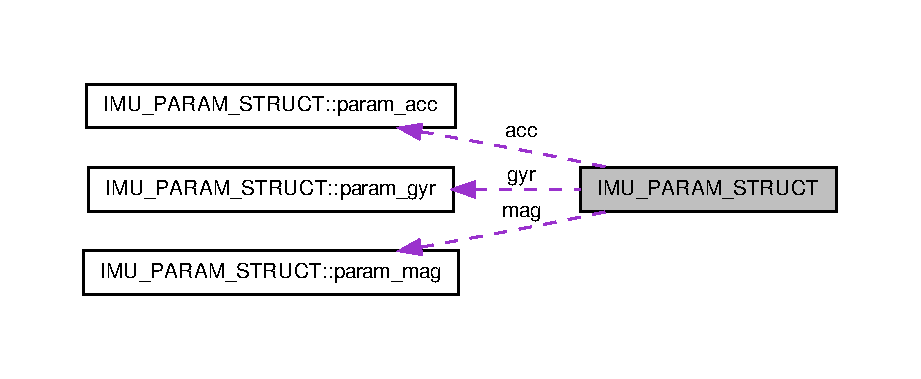
\includegraphics[width=350pt]{structIMU__PARAM__STRUCT__coll__graph}
\end{center}
\end{figure}
\subsection*{Data Structures}
\begin{DoxyCompactItemize}
\item 
struct \hyperlink{structIMU__PARAM__STRUCT_1_1param__acc}{param\-\_\-acc}
\begin{DoxyCompactList}\small\item\em Accelerometer Parameters. \end{DoxyCompactList}\item 
struct \hyperlink{structIMU__PARAM__STRUCT_1_1param__gyr}{param\-\_\-gyr}
\begin{DoxyCompactList}\small\item\em Gyrometer Parameters. \end{DoxyCompactList}\item 
struct \hyperlink{structIMU__PARAM__STRUCT_1_1param__mag}{param\-\_\-mag}
\begin{DoxyCompactList}\small\item\em Magnetometer Parameters. \end{DoxyCompactList}\end{DoxyCompactItemize}
\subsection*{Data Fields}
\begin{DoxyCompactItemize}
\item 
struct \hyperlink{structIMU__PARAM__STRUCT_1_1param__acc}{I\-M\-U\-\_\-\-P\-A\-R\-A\-M\-\_\-\-S\-T\-R\-U\-C\-T\-::param\-\_\-acc} \hyperlink{structIMU__PARAM__STRUCT_a92172e4757d0f8f9135a659e406c12e5}{acc}
\item 
struct \hyperlink{structIMU__PARAM__STRUCT_1_1param__gyr}{I\-M\-U\-\_\-\-P\-A\-R\-A\-M\-\_\-\-S\-T\-R\-U\-C\-T\-::param\-\_\-gyr} \hyperlink{structIMU__PARAM__STRUCT_a5a4557868f1af679a1098808397b02ec}{gyr}
\item 
struct \hyperlink{structIMU__PARAM__STRUCT_1_1param__mag}{I\-M\-U\-\_\-\-P\-A\-R\-A\-M\-\_\-\-S\-T\-R\-U\-C\-T\-::param\-\_\-mag} \hyperlink{structIMU__PARAM__STRUCT_a26b277dcaf05f3842995df888225f6f4}{mag}
\item 
int \hyperlink{structIMU__PARAM__STRUCT_a8a870f383fc9ba0b682fdc9b8c0d2734}{i2c\-\_\-dev}
\end{DoxyCompactItemize}


\subsection{Detailed Description}
Configs of I\-M\-U. 

Definition at line 31 of file communication.\-h.



\subsection{Field Documentation}
\hypertarget{structIMU__PARAM__STRUCT_a92172e4757d0f8f9135a659e406c12e5}{\index{I\-M\-U\-\_\-\-P\-A\-R\-A\-M\-\_\-\-S\-T\-R\-U\-C\-T@{I\-M\-U\-\_\-\-P\-A\-R\-A\-M\-\_\-\-S\-T\-R\-U\-C\-T}!acc@{acc}}
\index{acc@{acc}!IMU_PARAM_STRUCT@{I\-M\-U\-\_\-\-P\-A\-R\-A\-M\-\_\-\-S\-T\-R\-U\-C\-T}}
\subsubsection[{acc}]{\setlength{\rightskip}{0pt plus 5cm}struct {\bf I\-M\-U\-\_\-\-P\-A\-R\-A\-M\-\_\-\-S\-T\-R\-U\-C\-T\-::param\-\_\-acc} I\-M\-U\-\_\-\-P\-A\-R\-A\-M\-\_\-\-S\-T\-R\-U\-C\-T\-::acc}}\label{structIMU__PARAM__STRUCT_a92172e4757d0f8f9135a659e406c12e5}


Referenced by devices\-\_\-init(), and main().

\hypertarget{structIMU__PARAM__STRUCT_a5a4557868f1af679a1098808397b02ec}{\index{I\-M\-U\-\_\-\-P\-A\-R\-A\-M\-\_\-\-S\-T\-R\-U\-C\-T@{I\-M\-U\-\_\-\-P\-A\-R\-A\-M\-\_\-\-S\-T\-R\-U\-C\-T}!gyr@{gyr}}
\index{gyr@{gyr}!IMU_PARAM_STRUCT@{I\-M\-U\-\_\-\-P\-A\-R\-A\-M\-\_\-\-S\-T\-R\-U\-C\-T}}
\subsubsection[{gyr}]{\setlength{\rightskip}{0pt plus 5cm}struct {\bf I\-M\-U\-\_\-\-P\-A\-R\-A\-M\-\_\-\-S\-T\-R\-U\-C\-T\-::param\-\_\-gyr} I\-M\-U\-\_\-\-P\-A\-R\-A\-M\-\_\-\-S\-T\-R\-U\-C\-T\-::gyr}}\label{structIMU__PARAM__STRUCT_a5a4557868f1af679a1098808397b02ec}


Referenced by devices\-\_\-init(), and main().

\hypertarget{structIMU__PARAM__STRUCT_a8a870f383fc9ba0b682fdc9b8c0d2734}{\index{I\-M\-U\-\_\-\-P\-A\-R\-A\-M\-\_\-\-S\-T\-R\-U\-C\-T@{I\-M\-U\-\_\-\-P\-A\-R\-A\-M\-\_\-\-S\-T\-R\-U\-C\-T}!i2c\-\_\-dev@{i2c\-\_\-dev}}
\index{i2c\-\_\-dev@{i2c\-\_\-dev}!IMU_PARAM_STRUCT@{I\-M\-U\-\_\-\-P\-A\-R\-A\-M\-\_\-\-S\-T\-R\-U\-C\-T}}
\subsubsection[{i2c\-\_\-dev}]{\setlength{\rightskip}{0pt plus 5cm}int I\-M\-U\-\_\-\-P\-A\-R\-A\-M\-\_\-\-S\-T\-R\-U\-C\-T\-::i2c\-\_\-dev}}\label{structIMU__PARAM__STRUCT_a8a870f383fc9ba0b682fdc9b8c0d2734}


Definition at line 59 of file communication.\-h.



Referenced by devices\-\_\-init(), main(), periodic\-\_\-task\-\_\-1(), and periodic\-\_\-task\-\_\-2().

\hypertarget{structIMU__PARAM__STRUCT_a26b277dcaf05f3842995df888225f6f4}{\index{I\-M\-U\-\_\-\-P\-A\-R\-A\-M\-\_\-\-S\-T\-R\-U\-C\-T@{I\-M\-U\-\_\-\-P\-A\-R\-A\-M\-\_\-\-S\-T\-R\-U\-C\-T}!mag@{mag}}
\index{mag@{mag}!IMU_PARAM_STRUCT@{I\-M\-U\-\_\-\-P\-A\-R\-A\-M\-\_\-\-S\-T\-R\-U\-C\-T}}
\subsubsection[{mag}]{\setlength{\rightskip}{0pt plus 5cm}struct {\bf I\-M\-U\-\_\-\-P\-A\-R\-A\-M\-\_\-\-S\-T\-R\-U\-C\-T\-::param\-\_\-mag} I\-M\-U\-\_\-\-P\-A\-R\-A\-M\-\_\-\-S\-T\-R\-U\-C\-T\-::mag}}\label{structIMU__PARAM__STRUCT_a26b277dcaf05f3842995df888225f6f4}


Referenced by main().



The documentation for this struct was generated from the following file\-:\begin{DoxyCompactItemize}
\item 
communication/\hyperlink{communication_2communication_8h}{communication.\-h}\end{DoxyCompactItemize}

\hypertarget{structMATLAB__DATAHEAD}{\section{M\-A\-T\-L\-A\-B\-\_\-\-D\-A\-T\-A\-H\-E\-A\-D Struct Reference}
\label{structMATLAB__DATAHEAD}\index{M\-A\-T\-L\-A\-B\-\_\-\-D\-A\-T\-A\-H\-E\-A\-D@{M\-A\-T\-L\-A\-B\-\_\-\-D\-A\-T\-A\-H\-E\-A\-D}}
}
\subsection*{Data Fields}
\begin{DoxyCompactItemize}
\item 
long \hyperlink{structMATLAB__DATAHEAD_ad3587e58da5ca6cbe3cd98d5e2f46202}{type}
\item 
long \hyperlink{structMATLAB__DATAHEAD_abf1ef02c93522915bd7fdf9f72df44b7}{mrows}
\item 
long \hyperlink{structMATLAB__DATAHEAD_ae87d8eca5290fa03d01c79061498626f}{ncols}
\item 
long \hyperlink{structMATLAB__DATAHEAD_a7831e4f01682863fce4ba98071a7db08}{imagf}
\item 
long \hyperlink{structMATLAB__DATAHEAD_ad6e65844dcff1eb1cf7bf8752ba9a91c}{namlen}
\end{DoxyCompactItemize}


\subsection{Detailed Description}


Definition at line 13 of file gmatlabdatafile.\-c.



\subsection{Field Documentation}
\hypertarget{structMATLAB__DATAHEAD_a7831e4f01682863fce4ba98071a7db08}{\index{M\-A\-T\-L\-A\-B\-\_\-\-D\-A\-T\-A\-H\-E\-A\-D@{M\-A\-T\-L\-A\-B\-\_\-\-D\-A\-T\-A\-H\-E\-A\-D}!imagf@{imagf}}
\index{imagf@{imagf}!MATLAB_DATAHEAD@{M\-A\-T\-L\-A\-B\-\_\-\-D\-A\-T\-A\-H\-E\-A\-D}}
\subsubsection[{imagf}]{\setlength{\rightskip}{0pt plus 5cm}long M\-A\-T\-L\-A\-B\-\_\-\-D\-A\-T\-A\-H\-E\-A\-D\-::imagf}}\label{structMATLAB__DATAHEAD_a7831e4f01682863fce4ba98071a7db08}


Definition at line 17 of file gmatlabdatafile.\-c.



Referenced by g\-M\-A\-T\-L\-A\-B\-Data\-File\-\_\-\-Save\-Matrix(), and g\-M\-A\-T\-L\-A\-B\-Data\-File\-\_\-\-Save\-Vector().

\hypertarget{structMATLAB__DATAHEAD_abf1ef02c93522915bd7fdf9f72df44b7}{\index{M\-A\-T\-L\-A\-B\-\_\-\-D\-A\-T\-A\-H\-E\-A\-D@{M\-A\-T\-L\-A\-B\-\_\-\-D\-A\-T\-A\-H\-E\-A\-D}!mrows@{mrows}}
\index{mrows@{mrows}!MATLAB_DATAHEAD@{M\-A\-T\-L\-A\-B\-\_\-\-D\-A\-T\-A\-H\-E\-A\-D}}
\subsubsection[{mrows}]{\setlength{\rightskip}{0pt plus 5cm}long M\-A\-T\-L\-A\-B\-\_\-\-D\-A\-T\-A\-H\-E\-A\-D\-::mrows}}\label{structMATLAB__DATAHEAD_abf1ef02c93522915bd7fdf9f72df44b7}


Definition at line 15 of file gmatlabdatafile.\-c.



Referenced by g\-M\-A\-T\-L\-A\-B\-Data\-File\-\_\-\-Save\-Matrix(), and g\-M\-A\-T\-L\-A\-B\-Data\-File\-\_\-\-Save\-Vector().

\hypertarget{structMATLAB__DATAHEAD_ad6e65844dcff1eb1cf7bf8752ba9a91c}{\index{M\-A\-T\-L\-A\-B\-\_\-\-D\-A\-T\-A\-H\-E\-A\-D@{M\-A\-T\-L\-A\-B\-\_\-\-D\-A\-T\-A\-H\-E\-A\-D}!namlen@{namlen}}
\index{namlen@{namlen}!MATLAB_DATAHEAD@{M\-A\-T\-L\-A\-B\-\_\-\-D\-A\-T\-A\-H\-E\-A\-D}}
\subsubsection[{namlen}]{\setlength{\rightskip}{0pt plus 5cm}long M\-A\-T\-L\-A\-B\-\_\-\-D\-A\-T\-A\-H\-E\-A\-D\-::namlen}}\label{structMATLAB__DATAHEAD_ad6e65844dcff1eb1cf7bf8752ba9a91c}


Definition at line 18 of file gmatlabdatafile.\-c.



Referenced by g\-M\-A\-T\-L\-A\-B\-Data\-File\-\_\-\-Save\-Matrix(), and g\-M\-A\-T\-L\-A\-B\-Data\-File\-\_\-\-Save\-Vector().

\hypertarget{structMATLAB__DATAHEAD_ae87d8eca5290fa03d01c79061498626f}{\index{M\-A\-T\-L\-A\-B\-\_\-\-D\-A\-T\-A\-H\-E\-A\-D@{M\-A\-T\-L\-A\-B\-\_\-\-D\-A\-T\-A\-H\-E\-A\-D}!ncols@{ncols}}
\index{ncols@{ncols}!MATLAB_DATAHEAD@{M\-A\-T\-L\-A\-B\-\_\-\-D\-A\-T\-A\-H\-E\-A\-D}}
\subsubsection[{ncols}]{\setlength{\rightskip}{0pt plus 5cm}long M\-A\-T\-L\-A\-B\-\_\-\-D\-A\-T\-A\-H\-E\-A\-D\-::ncols}}\label{structMATLAB__DATAHEAD_ae87d8eca5290fa03d01c79061498626f}


Definition at line 16 of file gmatlabdatafile.\-c.



Referenced by g\-M\-A\-T\-L\-A\-B\-Data\-File\-\_\-\-Save\-Matrix(), and g\-M\-A\-T\-L\-A\-B\-Data\-File\-\_\-\-Save\-Vector().

\hypertarget{structMATLAB__DATAHEAD_ad3587e58da5ca6cbe3cd98d5e2f46202}{\index{M\-A\-T\-L\-A\-B\-\_\-\-D\-A\-T\-A\-H\-E\-A\-D@{M\-A\-T\-L\-A\-B\-\_\-\-D\-A\-T\-A\-H\-E\-A\-D}!type@{type}}
\index{type@{type}!MATLAB_DATAHEAD@{M\-A\-T\-L\-A\-B\-\_\-\-D\-A\-T\-A\-H\-E\-A\-D}}
\subsubsection[{type}]{\setlength{\rightskip}{0pt plus 5cm}long M\-A\-T\-L\-A\-B\-\_\-\-D\-A\-T\-A\-H\-E\-A\-D\-::type}}\label{structMATLAB__DATAHEAD_ad3587e58da5ca6cbe3cd98d5e2f46202}


Definition at line 14 of file gmatlabdatafile.\-c.



Referenced by g\-M\-A\-T\-L\-A\-B\-Data\-File\-\_\-\-Save\-Matrix(), and g\-M\-A\-T\-L\-A\-B\-Data\-File\-\_\-\-Save\-Vector().



The documentation for this struct was generated from the following file\-:\begin{DoxyCompactItemize}
\item 
gdatalogger/\hyperlink{gmatlabdatafile_8c}{gmatlabdatafile.\-c}\end{DoxyCompactItemize}

\hypertarget{structMRA__DATA__STRUCT}{\section{M\-R\-A\-\_\-\-D\-A\-T\-A\-\_\-\-S\-T\-R\-U\-C\-T Struct Reference}
\label{structMRA__DATA__STRUCT}\index{M\-R\-A\-\_\-\-D\-A\-T\-A\-\_\-\-S\-T\-R\-U\-C\-T@{M\-R\-A\-\_\-\-D\-A\-T\-A\-\_\-\-S\-T\-R\-U\-C\-T}}
}


Struct to control M\-R\-A.  




{\ttfamily \#include \char`\"{}communication.\-h\char`\"{}}

\subsection*{Data Fields}
\begin{DoxyCompactItemize}
\item 
short int \hyperlink{structMRA__DATA__STRUCT_a64b4e6bb604e58de593a60c87942b966}{v\-\_\-ctl}
\begin{DoxyCompactList}\small\item\em Voltage level for control output. \end{DoxyCompactList}\item 
short int \hyperlink{structMRA__DATA__STRUCT_a3a31d57268c33b21ac915fdc27dfe474}{v\-\_\-ctl\-\_\-read}
\begin{DoxyCompactList}\small\item\em Voltage level read from the actuator. \end{DoxyCompactList}\item 
int \hyperlink{structMRA__DATA__STRUCT_afca6e851d302f3a786885a4e1eec79d7}{new\-\_\-data}
\begin{DoxyCompactList}\small\item\em ?? \end{DoxyCompactList}\item 
int \hyperlink{structMRA__DATA__STRUCT_a5b1af89ee717f5b14c18e8ac12e93e75}{new\-\_\-ctl}
\begin{DoxyCompactList}\small\item\em ?? \end{DoxyCompactList}\end{DoxyCompactItemize}


\subsection{Detailed Description}
Struct to control M\-R\-A. 

Definition at line 126 of file communication.\-h.



\subsection{Field Documentation}
\hypertarget{structMRA__DATA__STRUCT_a5b1af89ee717f5b14c18e8ac12e93e75}{\index{M\-R\-A\-\_\-\-D\-A\-T\-A\-\_\-\-S\-T\-R\-U\-C\-T@{M\-R\-A\-\_\-\-D\-A\-T\-A\-\_\-\-S\-T\-R\-U\-C\-T}!new\-\_\-ctl@{new\-\_\-ctl}}
\index{new\-\_\-ctl@{new\-\_\-ctl}!MRA_DATA_STRUCT@{M\-R\-A\-\_\-\-D\-A\-T\-A\-\_\-\-S\-T\-R\-U\-C\-T}}
\subsubsection[{new\-\_\-ctl}]{\setlength{\rightskip}{0pt plus 5cm}int M\-R\-A\-\_\-\-D\-A\-T\-A\-\_\-\-S\-T\-R\-U\-C\-T\-::new\-\_\-ctl}}\label{structMRA__DATA__STRUCT_a5b1af89ee717f5b14c18e8ac12e93e75}


?? 



Definition at line 130 of file communication.\-h.



Referenced by actuate(), and devices\-\_\-init().

\hypertarget{structMRA__DATA__STRUCT_afca6e851d302f3a786885a4e1eec79d7}{\index{M\-R\-A\-\_\-\-D\-A\-T\-A\-\_\-\-S\-T\-R\-U\-C\-T@{M\-R\-A\-\_\-\-D\-A\-T\-A\-\_\-\-S\-T\-R\-U\-C\-T}!new\-\_\-data@{new\-\_\-data}}
\index{new\-\_\-data@{new\-\_\-data}!MRA_DATA_STRUCT@{M\-R\-A\-\_\-\-D\-A\-T\-A\-\_\-\-S\-T\-R\-U\-C\-T}}
\subsubsection[{new\-\_\-data}]{\setlength{\rightskip}{0pt plus 5cm}int M\-R\-A\-\_\-\-D\-A\-T\-A\-\_\-\-S\-T\-R\-U\-C\-T\-::new\-\_\-data}}\label{structMRA__DATA__STRUCT_afca6e851d302f3a786885a4e1eec79d7}


?? 



Definition at line 129 of file communication.\-h.



Referenced by read\-\_\-all\-\_\-data().

\hypertarget{structMRA__DATA__STRUCT_a64b4e6bb604e58de593a60c87942b966}{\index{M\-R\-A\-\_\-\-D\-A\-T\-A\-\_\-\-S\-T\-R\-U\-C\-T@{M\-R\-A\-\_\-\-D\-A\-T\-A\-\_\-\-S\-T\-R\-U\-C\-T}!v\-\_\-ctl@{v\-\_\-ctl}}
\index{v\-\_\-ctl@{v\-\_\-ctl}!MRA_DATA_STRUCT@{M\-R\-A\-\_\-\-D\-A\-T\-A\-\_\-\-S\-T\-R\-U\-C\-T}}
\subsubsection[{v\-\_\-ctl}]{\setlength{\rightskip}{0pt plus 5cm}short int M\-R\-A\-\_\-\-D\-A\-T\-A\-\_\-\-S\-T\-R\-U\-C\-T\-::v\-\_\-ctl}}\label{structMRA__DATA__STRUCT_a64b4e6bb604e58de593a60c87942b966}


Voltage level for control output. 



Definition at line 127 of file communication.\-h.



Referenced by actuate(), control\-\_\-main(), datalogger\-\_\-update(), devices\-\_\-init(), periodic\-\_\-task\-\_\-1(), ui\-\_\-mra\-\_\-data(), and ui\-\_\-overview\-\_\-data().

\hypertarget{structMRA__DATA__STRUCT_a3a31d57268c33b21ac915fdc27dfe474}{\index{M\-R\-A\-\_\-\-D\-A\-T\-A\-\_\-\-S\-T\-R\-U\-C\-T@{M\-R\-A\-\_\-\-D\-A\-T\-A\-\_\-\-S\-T\-R\-U\-C\-T}!v\-\_\-ctl\-\_\-read@{v\-\_\-ctl\-\_\-read}}
\index{v\-\_\-ctl\-\_\-read@{v\-\_\-ctl\-\_\-read}!MRA_DATA_STRUCT@{M\-R\-A\-\_\-\-D\-A\-T\-A\-\_\-\-S\-T\-R\-U\-C\-T}}
\subsubsection[{v\-\_\-ctl\-\_\-read}]{\setlength{\rightskip}{0pt plus 5cm}short int M\-R\-A\-\_\-\-D\-A\-T\-A\-\_\-\-S\-T\-R\-U\-C\-T\-::v\-\_\-ctl\-\_\-read}}\label{structMRA__DATA__STRUCT_a3a31d57268c33b21ac915fdc27dfe474}


Voltage level read from the actuator. 



Definition at line 128 of file communication.\-h.



Referenced by datalogger\-\_\-update(), read\-\_\-all\-\_\-data(), ui\-\_\-mra\-\_\-data(), and ui\-\_\-overview\-\_\-data().



The documentation for this struct was generated from the following file\-:\begin{DoxyCompactItemize}
\item 
communication/\hyperlink{communication_2communication_8h}{communication.\-h}\end{DoxyCompactItemize}

\hypertarget{structIMU__PARAM__STRUCT_1_1param__acc}{\section{I\-M\-U\-\_\-\-P\-A\-R\-A\-M\-\_\-\-S\-T\-R\-U\-C\-T\-:\-:param\-\_\-acc Struct Reference}
\label{structIMU__PARAM__STRUCT_1_1param__acc}\index{I\-M\-U\-\_\-\-P\-A\-R\-A\-M\-\_\-\-S\-T\-R\-U\-C\-T\-::param\-\_\-acc@{I\-M\-U\-\_\-\-P\-A\-R\-A\-M\-\_\-\-S\-T\-R\-U\-C\-T\-::param\-\_\-acc}}
}


Accelerometer Parameters.  




{\ttfamily \#include \char`\"{}communication.\-h\char`\"{}}

\subsection*{Data Fields}
\begin{DoxyCompactItemize}
\item 
uint8\-\_\-t \hyperlink{structIMU__PARAM__STRUCT_1_1param__acc_af57da5d956ffa7e49a184326b6b9c738}{full\-\_\-res}
\item 
uint16\-\_\-t \hyperlink{structIMU__PARAM__STRUCT_1_1param__acc_a30e6a318cad098cd8379416705820f95}{rate}
\item 
uint8\-\_\-t \hyperlink{structIMU__PARAM__STRUCT_1_1param__acc_a26199b298ef2d353192dfbc706bce8cf}{range}
\end{DoxyCompactItemize}


\subsection{Detailed Description}
Accelerometer Parameters. 

Definition at line 35 of file communication.\-h.



\subsection{Field Documentation}
\hypertarget{structIMU__PARAM__STRUCT_1_1param__acc_af57da5d956ffa7e49a184326b6b9c738}{\index{I\-M\-U\-\_\-\-P\-A\-R\-A\-M\-\_\-\-S\-T\-R\-U\-C\-T\-::param\-\_\-acc@{I\-M\-U\-\_\-\-P\-A\-R\-A\-M\-\_\-\-S\-T\-R\-U\-C\-T\-::param\-\_\-acc}!full\-\_\-res@{full\-\_\-res}}
\index{full\-\_\-res@{full\-\_\-res}!IMU_PARAM_STRUCT::param_acc@{I\-M\-U\-\_\-\-P\-A\-R\-A\-M\-\_\-\-S\-T\-R\-U\-C\-T\-::param\-\_\-acc}}
\subsubsection[{full\-\_\-res}]{\setlength{\rightskip}{0pt plus 5cm}uint8\-\_\-t I\-M\-U\-\_\-\-P\-A\-R\-A\-M\-\_\-\-S\-T\-R\-U\-C\-T\-::param\-\_\-acc\-::full\-\_\-res}}\label{structIMU__PARAM__STRUCT_1_1param__acc_af57da5d956ffa7e49a184326b6b9c738}


Definition at line 36 of file communication.\-h.



Referenced by devices\-\_\-init(), and main().

\hypertarget{structIMU__PARAM__STRUCT_1_1param__acc_a26199b298ef2d353192dfbc706bce8cf}{\index{I\-M\-U\-\_\-\-P\-A\-R\-A\-M\-\_\-\-S\-T\-R\-U\-C\-T\-::param\-\_\-acc@{I\-M\-U\-\_\-\-P\-A\-R\-A\-M\-\_\-\-S\-T\-R\-U\-C\-T\-::param\-\_\-acc}!range@{range}}
\index{range@{range}!IMU_PARAM_STRUCT::param_acc@{I\-M\-U\-\_\-\-P\-A\-R\-A\-M\-\_\-\-S\-T\-R\-U\-C\-T\-::param\-\_\-acc}}
\subsubsection[{range}]{\setlength{\rightskip}{0pt plus 5cm}uint8\-\_\-t I\-M\-U\-\_\-\-P\-A\-R\-A\-M\-\_\-\-S\-T\-R\-U\-C\-T\-::param\-\_\-acc\-::range}}\label{structIMU__PARAM__STRUCT_1_1param__acc_a26199b298ef2d353192dfbc706bce8cf}


Definition at line 38 of file communication.\-h.



Referenced by devices\-\_\-init(), and main().

\hypertarget{structIMU__PARAM__STRUCT_1_1param__acc_a30e6a318cad098cd8379416705820f95}{\index{I\-M\-U\-\_\-\-P\-A\-R\-A\-M\-\_\-\-S\-T\-R\-U\-C\-T\-::param\-\_\-acc@{I\-M\-U\-\_\-\-P\-A\-R\-A\-M\-\_\-\-S\-T\-R\-U\-C\-T\-::param\-\_\-acc}!rate@{rate}}
\index{rate@{rate}!IMU_PARAM_STRUCT::param_acc@{I\-M\-U\-\_\-\-P\-A\-R\-A\-M\-\_\-\-S\-T\-R\-U\-C\-T\-::param\-\_\-acc}}
\subsubsection[{rate}]{\setlength{\rightskip}{0pt plus 5cm}uint16\-\_\-t I\-M\-U\-\_\-\-P\-A\-R\-A\-M\-\_\-\-S\-T\-R\-U\-C\-T\-::param\-\_\-acc\-::rate}}\label{structIMU__PARAM__STRUCT_1_1param__acc_a30e6a318cad098cd8379416705820f95}


Definition at line 37 of file communication.\-h.



Referenced by devices\-\_\-init(), and main().



The documentation for this struct was generated from the following file\-:\begin{DoxyCompactItemize}
\item 
communication/\hyperlink{communication_2communication_8h}{communication.\-h}\end{DoxyCompactItemize}

\hypertarget{structIMU__PARAM__STRUCT_1_1param__gyr}{\section{I\-M\-U\-\_\-\-P\-A\-R\-A\-M\-\_\-\-S\-T\-R\-U\-C\-T\-:\-:param\-\_\-gyr Struct Reference}
\label{structIMU__PARAM__STRUCT_1_1param__gyr}\index{I\-M\-U\-\_\-\-P\-A\-R\-A\-M\-\_\-\-S\-T\-R\-U\-C\-T\-::param\-\_\-gyr@{I\-M\-U\-\_\-\-P\-A\-R\-A\-M\-\_\-\-S\-T\-R\-U\-C\-T\-::param\-\_\-gyr}}
}


Gyrometer Parameters.  




{\ttfamily \#include \char`\"{}communication.\-h\char`\"{}}

\subsection*{Data Fields}
\begin{DoxyCompactItemize}
\item 
float \hyperlink{structIMU__PARAM__STRUCT_1_1param__gyr_a5aa70e1e9634411c89aacfbc570cc91c}{rate}
\item 
short int \hyperlink{structIMU__PARAM__STRUCT_1_1param__gyr_aa612f7299b43a1bf1fc597688c2fa02d}{lpf\-\_\-bw}
\item 
char \hyperlink{structIMU__PARAM__STRUCT_1_1param__gyr_aca3b791cb480f2da4703d4c256a7de48}{clk\-\_\-source}
\item 
char $\ast$ \hyperlink{structIMU__PARAM__STRUCT_1_1param__gyr_a909d153e794ec443be04625ce00e4178}{act}
\end{DoxyCompactItemize}


\subsection{Detailed Description}
Gyrometer Parameters. 

Definition at line 43 of file communication.\-h.



\subsection{Field Documentation}
\hypertarget{structIMU__PARAM__STRUCT_1_1param__gyr_a909d153e794ec443be04625ce00e4178}{\index{I\-M\-U\-\_\-\-P\-A\-R\-A\-M\-\_\-\-S\-T\-R\-U\-C\-T\-::param\-\_\-gyr@{I\-M\-U\-\_\-\-P\-A\-R\-A\-M\-\_\-\-S\-T\-R\-U\-C\-T\-::param\-\_\-gyr}!act@{act}}
\index{act@{act}!IMU_PARAM_STRUCT::param_gyr@{I\-M\-U\-\_\-\-P\-A\-R\-A\-M\-\_\-\-S\-T\-R\-U\-C\-T\-::param\-\_\-gyr}}
\subsubsection[{act}]{\setlength{\rightskip}{0pt plus 5cm}char$\ast$ I\-M\-U\-\_\-\-P\-A\-R\-A\-M\-\_\-\-S\-T\-R\-U\-C\-T\-::param\-\_\-gyr\-::act}}\label{structIMU__PARAM__STRUCT_1_1param__gyr_a909d153e794ec443be04625ce00e4178}


Definition at line 47 of file communication.\-h.



Referenced by devices\-\_\-init(), and main().

\hypertarget{structIMU__PARAM__STRUCT_1_1param__gyr_aca3b791cb480f2da4703d4c256a7de48}{\index{I\-M\-U\-\_\-\-P\-A\-R\-A\-M\-\_\-\-S\-T\-R\-U\-C\-T\-::param\-\_\-gyr@{I\-M\-U\-\_\-\-P\-A\-R\-A\-M\-\_\-\-S\-T\-R\-U\-C\-T\-::param\-\_\-gyr}!clk\-\_\-source@{clk\-\_\-source}}
\index{clk\-\_\-source@{clk\-\_\-source}!IMU_PARAM_STRUCT::param_gyr@{I\-M\-U\-\_\-\-P\-A\-R\-A\-M\-\_\-\-S\-T\-R\-U\-C\-T\-::param\-\_\-gyr}}
\subsubsection[{clk\-\_\-source}]{\setlength{\rightskip}{0pt plus 5cm}char I\-M\-U\-\_\-\-P\-A\-R\-A\-M\-\_\-\-S\-T\-R\-U\-C\-T\-::param\-\_\-gyr\-::clk\-\_\-source}}\label{structIMU__PARAM__STRUCT_1_1param__gyr_aca3b791cb480f2da4703d4c256a7de48}


Definition at line 46 of file communication.\-h.



Referenced by devices\-\_\-init(), and main().

\hypertarget{structIMU__PARAM__STRUCT_1_1param__gyr_aa612f7299b43a1bf1fc597688c2fa02d}{\index{I\-M\-U\-\_\-\-P\-A\-R\-A\-M\-\_\-\-S\-T\-R\-U\-C\-T\-::param\-\_\-gyr@{I\-M\-U\-\_\-\-P\-A\-R\-A\-M\-\_\-\-S\-T\-R\-U\-C\-T\-::param\-\_\-gyr}!lpf\-\_\-bw@{lpf\-\_\-bw}}
\index{lpf\-\_\-bw@{lpf\-\_\-bw}!IMU_PARAM_STRUCT::param_gyr@{I\-M\-U\-\_\-\-P\-A\-R\-A\-M\-\_\-\-S\-T\-R\-U\-C\-T\-::param\-\_\-gyr}}
\subsubsection[{lpf\-\_\-bw}]{\setlength{\rightskip}{0pt plus 5cm}short int I\-M\-U\-\_\-\-P\-A\-R\-A\-M\-\_\-\-S\-T\-R\-U\-C\-T\-::param\-\_\-gyr\-::lpf\-\_\-bw}}\label{structIMU__PARAM__STRUCT_1_1param__gyr_aa612f7299b43a1bf1fc597688c2fa02d}


Definition at line 45 of file communication.\-h.



Referenced by devices\-\_\-init(), and main().

\hypertarget{structIMU__PARAM__STRUCT_1_1param__gyr_a5aa70e1e9634411c89aacfbc570cc91c}{\index{I\-M\-U\-\_\-\-P\-A\-R\-A\-M\-\_\-\-S\-T\-R\-U\-C\-T\-::param\-\_\-gyr@{I\-M\-U\-\_\-\-P\-A\-R\-A\-M\-\_\-\-S\-T\-R\-U\-C\-T\-::param\-\_\-gyr}!rate@{rate}}
\index{rate@{rate}!IMU_PARAM_STRUCT::param_gyr@{I\-M\-U\-\_\-\-P\-A\-R\-A\-M\-\_\-\-S\-T\-R\-U\-C\-T\-::param\-\_\-gyr}}
\subsubsection[{rate}]{\setlength{\rightskip}{0pt plus 5cm}float I\-M\-U\-\_\-\-P\-A\-R\-A\-M\-\_\-\-S\-T\-R\-U\-C\-T\-::param\-\_\-gyr\-::rate}}\label{structIMU__PARAM__STRUCT_1_1param__gyr_a5aa70e1e9634411c89aacfbc570cc91c}


Definition at line 44 of file communication.\-h.



Referenced by devices\-\_\-init(), and main().



The documentation for this struct was generated from the following file\-:\begin{DoxyCompactItemize}
\item 
communication/\hyperlink{communication_2communication_8h}{communication.\-h}\end{DoxyCompactItemize}

\hypertarget{structIMU__PARAM__STRUCT_1_1param__mag}{
\section{IMU\_\-PARAM\_\-STRUCT::param\_\-mag Struct Reference}
\label{structIMU__PARAM__STRUCT_1_1param__mag}\index{IMU\_\-PARAM\_\-STRUCT::param\_\-mag@{IMU\_\-PARAM\_\-STRUCT::param\_\-mag}}
}
\subsection*{Data Fields}
\begin{DoxyCompactItemize}
\item 
\hypertarget{structIMU__PARAM__STRUCT_1_1param__mag_a234de95423b604b05b851ef90890cea1}{
uint8\_\-t {\bfseries rate}}
\label{structIMU__PARAM__STRUCT_1_1param__mag_a234de95423b604b05b851ef90890cea1}

\item 
\hypertarget{structIMU__PARAM__STRUCT_1_1param__mag_a40ad27ebdb5fde35257b1dc52e40f476}{
uint8\_\-t {\bfseries range}}
\label{structIMU__PARAM__STRUCT_1_1param__mag_a40ad27ebdb5fde35257b1dc52e40f476}

\item 
\hypertarget{structIMU__PARAM__STRUCT_1_1param__mag_a52c22cae6940eb39fb72aca66cfeba9a}{
uint8\_\-t {\bfseries samples\_\-avg}}
\label{structIMU__PARAM__STRUCT_1_1param__mag_a52c22cae6940eb39fb72aca66cfeba9a}

\item 
\hypertarget{structIMU__PARAM__STRUCT_1_1param__mag_a1f3536709c05310005d648f339d70c54}{
uint8\_\-t {\bfseries meas\_\-mode}}
\label{structIMU__PARAM__STRUCT_1_1param__mag_a1f3536709c05310005d648f339d70c54}

\item 
\hypertarget{structIMU__PARAM__STRUCT_1_1param__mag_a39b83b3e9ff5bdcafed0bdf6a2de584b}{
uint8\_\-t {\bfseries op\_\-mode}}
\label{structIMU__PARAM__STRUCT_1_1param__mag_a39b83b3e9ff5bdcafed0bdf6a2de584b}

\end{DoxyCompactItemize}


The documentation for this struct was generated from the following files:\begin{DoxyCompactItemize}
\item 
communication/communication (Cópia em conflito de Caio Gustavo Mesquita Angelo 2013-\/05-\/17).h\item 
communication/communication.h\end{DoxyCompactItemize}

\hypertarget{structSPI__PARAM__STRUCT}{\section{S\-P\-I\-\_\-\-P\-A\-R\-A\-M\-\_\-\-S\-T\-R\-U\-C\-T Struct Reference}
\label{structSPI__PARAM__STRUCT}\index{S\-P\-I\-\_\-\-P\-A\-R\-A\-M\-\_\-\-S\-T\-R\-U\-C\-T@{S\-P\-I\-\_\-\-P\-A\-R\-A\-M\-\_\-\-S\-T\-R\-U\-C\-T}}
}


Configs for S\-P\-I.  




{\ttfamily \#include \char`\"{}communication.\-h\char`\"{}}

\subsection*{Data Fields}
\begin{DoxyCompactItemize}
\item 
uint8\-\_\-t \hyperlink{structSPI__PARAM__STRUCT_a82c546c99f6c3daed73c1e23426be847}{mode}
\item 
uint32\-\_\-t \hyperlink{structSPI__PARAM__STRUCT_a53a8d386594a81eb9bc6f971bfe36c54}{speed}
\item 
uint8\-\_\-t \hyperlink{structSPI__PARAM__STRUCT_ae0d62e0a5554783d710b677a017e246f}{cs}
\item 
int \hyperlink{structSPI__PARAM__STRUCT_abe385c44333d268d17cf648c8e371cad}{spi\-\_\-dev}
\end{DoxyCompactItemize}


\subsection{Detailed Description}
Configs for S\-P\-I. 

Definition at line 65 of file communication.\-h.



\subsection{Field Documentation}
\hypertarget{structSPI__PARAM__STRUCT_ae0d62e0a5554783d710b677a017e246f}{\index{S\-P\-I\-\_\-\-P\-A\-R\-A\-M\-\_\-\-S\-T\-R\-U\-C\-T@{S\-P\-I\-\_\-\-P\-A\-R\-A\-M\-\_\-\-S\-T\-R\-U\-C\-T}!cs@{cs}}
\index{cs@{cs}!SPI_PARAM_STRUCT@{S\-P\-I\-\_\-\-P\-A\-R\-A\-M\-\_\-\-S\-T\-R\-U\-C\-T}}
\subsubsection[{cs}]{\setlength{\rightskip}{0pt plus 5cm}uint8\-\_\-t S\-P\-I\-\_\-\-P\-A\-R\-A\-M\-\_\-\-S\-T\-R\-U\-C\-T\-::cs}}\label{structSPI__PARAM__STRUCT_ae0d62e0a5554783d710b677a017e246f}


Definition at line 68 of file communication.\-h.



Referenced by devices\-\_\-init(), and main().

\hypertarget{structSPI__PARAM__STRUCT_a82c546c99f6c3daed73c1e23426be847}{\index{S\-P\-I\-\_\-\-P\-A\-R\-A\-M\-\_\-\-S\-T\-R\-U\-C\-T@{S\-P\-I\-\_\-\-P\-A\-R\-A\-M\-\_\-\-S\-T\-R\-U\-C\-T}!mode@{mode}}
\index{mode@{mode}!SPI_PARAM_STRUCT@{S\-P\-I\-\_\-\-P\-A\-R\-A\-M\-\_\-\-S\-T\-R\-U\-C\-T}}
\subsubsection[{mode}]{\setlength{\rightskip}{0pt plus 5cm}uint8\-\_\-t S\-P\-I\-\_\-\-P\-A\-R\-A\-M\-\_\-\-S\-T\-R\-U\-C\-T\-::mode}}\label{structSPI__PARAM__STRUCT_a82c546c99f6c3daed73c1e23426be847}


Definition at line 66 of file communication.\-h.



Referenced by devices\-\_\-init(), and main().

\hypertarget{structSPI__PARAM__STRUCT_a53a8d386594a81eb9bc6f971bfe36c54}{\index{S\-P\-I\-\_\-\-P\-A\-R\-A\-M\-\_\-\-S\-T\-R\-U\-C\-T@{S\-P\-I\-\_\-\-P\-A\-R\-A\-M\-\_\-\-S\-T\-R\-U\-C\-T}!speed@{speed}}
\index{speed@{speed}!SPI_PARAM_STRUCT@{S\-P\-I\-\_\-\-P\-A\-R\-A\-M\-\_\-\-S\-T\-R\-U\-C\-T}}
\subsubsection[{speed}]{\setlength{\rightskip}{0pt plus 5cm}uint32\-\_\-t S\-P\-I\-\_\-\-P\-A\-R\-A\-M\-\_\-\-S\-T\-R\-U\-C\-T\-::speed}}\label{structSPI__PARAM__STRUCT_a53a8d386594a81eb9bc6f971bfe36c54}


Definition at line 67 of file communication.\-h.



Referenced by devices\-\_\-init(), and main().

\hypertarget{structSPI__PARAM__STRUCT_abe385c44333d268d17cf648c8e371cad}{\index{S\-P\-I\-\_\-\-P\-A\-R\-A\-M\-\_\-\-S\-T\-R\-U\-C\-T@{S\-P\-I\-\_\-\-P\-A\-R\-A\-M\-\_\-\-S\-T\-R\-U\-C\-T}!spi\-\_\-dev@{spi\-\_\-dev}}
\index{spi\-\_\-dev@{spi\-\_\-dev}!SPI_PARAM_STRUCT@{S\-P\-I\-\_\-\-P\-A\-R\-A\-M\-\_\-\-S\-T\-R\-U\-C\-T}}
\subsubsection[{spi\-\_\-dev}]{\setlength{\rightskip}{0pt plus 5cm}int S\-P\-I\-\_\-\-P\-A\-R\-A\-M\-\_\-\-S\-T\-R\-U\-C\-T\-::spi\-\_\-dev}}\label{structSPI__PARAM__STRUCT_abe385c44333d268d17cf648c8e371cad}


Definition at line 69 of file communication.\-h.



Referenced by devices\-\_\-init(), main(), periodic\-\_\-task\-\_\-1(), and periodic\-\_\-task\-\_\-2().



The documentation for this struct was generated from the following file\-:\begin{DoxyCompactItemize}
\item 
communication/\hyperlink{communication_2communication_8h}{communication.\-h}\end{DoxyCompactItemize}

\hypertarget{structTASK__S}{
\section{TASK\_\-S Struct Reference}
\label{structTASK__S}\index{TASK\_\-S@{TASK\_\-S}}
}


Task to schedule definition.  




{\ttfamily \#include \char`\"{}taskScheduler.h\char`\"{}}

\subsection*{Data Fields}
\begin{DoxyCompactItemize}
\item 
timer\_\-t \hyperlink{structTASK__S_a17834f3d4f84241ccb4191f3cf7d7af3}{timer}
\item 
volatile double \hyperlink{structTASK__S_a29a175bdd4b9f880a2b69bb5186e3c7e}{t\_\-global}
\item 
volatile double \hyperlink{structTASK__S_ae06b712fd9963cff8192e9ef3140bc6d}{T\_\-exec\_\-global}
\item 
volatile double \hyperlink{structTASK__S_a9ebae87e1b64869f328a47473f2ea7d7}{T\_\-mean\_\-global}
\item 
volatile double \hyperlink{structTASK__S_a430c874cbf361b6dbc75ad1540880948}{T\_\-max\_\-global}
\item 
volatile double \hyperlink{structTASK__S_a07174e333a0013f4d51b30509b388f58}{T\_\-min\_\-global}
\item 
volatile int \hyperlink{structTASK__S_aabd8f80831e6cfd8e51bbd371eed907b}{period\_\-us}
\item 
volatile int \hyperlink{structTASK__S_a4b50404ee955691f1c62845cdc9de676}{isFirstExecution}
\begin{DoxyCompactList}\small\item\em Flag to sign first Exec. \item\end{DoxyCompactList}\item 
void($\ast$ \hyperlink{structTASK__S_a6ce7396d04fd08be26e2e8b75a276122}{run} )(int)
\begin{DoxyCompactList}\small\item\em hook to the action \item\end{DoxyCompactList}\end{DoxyCompactItemize}


\subsection{Detailed Description}
Task to schedule definition. 

Definition at line 20 of file taskScheduler.h.



\subsection{Field Documentation}
\hypertarget{structTASK__S_a4b50404ee955691f1c62845cdc9de676}{
\index{TASK\_\-S@{TASK\_\-S}!isFirstExecution@{isFirstExecution}}
\index{isFirstExecution@{isFirstExecution}!TASK_S@{TASK\_\-S}}
\subsubsection[{isFirstExecution}]{\setlength{\rightskip}{0pt plus 5cm}volatile int {\bf TASK\_\-S::isFirstExecution}}}
\label{structTASK__S_a4b50404ee955691f1c62845cdc9de676}


Flag to sign first Exec. 



Definition at line 28 of file taskScheduler.h.



Referenced by timer\_\-start\_\-task().

\hypertarget{structTASK__S_aabd8f80831e6cfd8e51bbd371eed907b}{
\index{TASK\_\-S@{TASK\_\-S}!period\_\-us@{period\_\-us}}
\index{period\_\-us@{period\_\-us}!TASK_S@{TASK\_\-S}}
\subsubsection[{period\_\-us}]{\setlength{\rightskip}{0pt plus 5cm}volatile int {\bf TASK\_\-S::period\_\-us}}}
\label{structTASK__S_aabd8f80831e6cfd8e51bbd371eed907b}


Definition at line 27 of file taskScheduler.h.



Referenced by get\_\-time(), and timer\_\-start\_\-task().

\hypertarget{structTASK__S_a6ce7396d04fd08be26e2e8b75a276122}{
\index{TASK\_\-S@{TASK\_\-S}!run@{run}}
\index{run@{run}!TASK_S@{TASK\_\-S}}
\subsubsection[{run}]{\setlength{\rightskip}{0pt plus 5cm}void($\ast$ {\bf TASK\_\-S::run})(int)}}
\label{structTASK__S_a6ce7396d04fd08be26e2e8b75a276122}


hook to the action 



Definition at line 30 of file taskScheduler.h.



Referenced by timer\_\-start\_\-task().

\hypertarget{structTASK__S_ae06b712fd9963cff8192e9ef3140bc6d}{
\index{TASK\_\-S@{TASK\_\-S}!T\_\-exec\_\-global@{T\_\-exec\_\-global}}
\index{T\_\-exec\_\-global@{T\_\-exec\_\-global}!TASK_S@{TASK\_\-S}}
\subsubsection[{T\_\-exec\_\-global}]{\setlength{\rightskip}{0pt plus 5cm}volatile double {\bf TASK\_\-S::T\_\-exec\_\-global}}}
\label{structTASK__S_ae06b712fd9963cff8192e9ef3140bc6d}


Definition at line 23 of file taskScheduler.h.

\hypertarget{structTASK__S_a29a175bdd4b9f880a2b69bb5186e3c7e}{
\index{TASK\_\-S@{TASK\_\-S}!t\_\-global@{t\_\-global}}
\index{t\_\-global@{t\_\-global}!TASK_S@{TASK\_\-S}}
\subsubsection[{t\_\-global}]{\setlength{\rightskip}{0pt plus 5cm}volatile double {\bf TASK\_\-S::t\_\-global}}}
\label{structTASK__S_a29a175bdd4b9f880a2b69bb5186e3c7e}


Definition at line 22 of file taskScheduler.h.



Referenced by control\_\-task(), and get\_\-time().

\hypertarget{structTASK__S_a430c874cbf361b6dbc75ad1540880948}{
\index{TASK\_\-S@{TASK\_\-S}!T\_\-max\_\-global@{T\_\-max\_\-global}}
\index{T\_\-max\_\-global@{T\_\-max\_\-global}!TASK_S@{TASK\_\-S}}
\subsubsection[{T\_\-max\_\-global}]{\setlength{\rightskip}{0pt plus 5cm}volatile double {\bf TASK\_\-S::T\_\-max\_\-global}}}
\label{structTASK__S_a430c874cbf361b6dbc75ad1540880948}


Definition at line 25 of file taskScheduler.h.

\hypertarget{structTASK__S_a9ebae87e1b64869f328a47473f2ea7d7}{
\index{TASK\_\-S@{TASK\_\-S}!T\_\-mean\_\-global@{T\_\-mean\_\-global}}
\index{T\_\-mean\_\-global@{T\_\-mean\_\-global}!TASK_S@{TASK\_\-S}}
\subsubsection[{T\_\-mean\_\-global}]{\setlength{\rightskip}{0pt plus 5cm}volatile double {\bf TASK\_\-S::T\_\-mean\_\-global}}}
\label{structTASK__S_a9ebae87e1b64869f328a47473f2ea7d7}


Definition at line 24 of file taskScheduler.h.



Referenced by get\_\-time().

\hypertarget{structTASK__S_a07174e333a0013f4d51b30509b388f58}{
\index{TASK\_\-S@{TASK\_\-S}!T\_\-min\_\-global@{T\_\-min\_\-global}}
\index{T\_\-min\_\-global@{T\_\-min\_\-global}!TASK_S@{TASK\_\-S}}
\subsubsection[{T\_\-min\_\-global}]{\setlength{\rightskip}{0pt plus 5cm}volatile double {\bf TASK\_\-S::T\_\-min\_\-global}}}
\label{structTASK__S_a07174e333a0013f4d51b30509b388f58}


Definition at line 26 of file taskScheduler.h.

\hypertarget{structTASK__S_a17834f3d4f84241ccb4191f3cf7d7af3}{
\index{TASK\_\-S@{TASK\_\-S}!timer@{timer}}
\index{timer@{timer}!TASK_S@{TASK\_\-S}}
\subsubsection[{timer}]{\setlength{\rightskip}{0pt plus 5cm}timer\_\-t {\bf TASK\_\-S::timer}}}
\label{structTASK__S_a17834f3d4f84241ccb4191f3cf7d7af3}


Definition at line 21 of file taskScheduler.h.



Referenced by timer\_\-start\_\-task().



The documentation for this struct was generated from the following file:\begin{DoxyCompactItemize}
\item 
\hyperlink{taskScheduler_8h}{taskScheduler.h}\end{DoxyCompactItemize}

\chapter{File Documentation}
\hypertarget{calibration_2calibration_8c}{\section{calibration/calibration.c File Reference}
\label{calibration_2calibration_8c}\index{calibration/calibration.\-c@{calibration/calibration.\-c}}
}
{\ttfamily \#include $<$stdio.\-h$>$}\\*
{\ttfamily \#include $<$stdlib.\-h$>$}\\*
{\ttfamily \#include \char`\"{}calibration.\-h\char`\"{}}\\*
Include dependency graph for calibration.\-c\-:\nopagebreak
\begin{figure}[H]
\begin{center}
\leavevmode
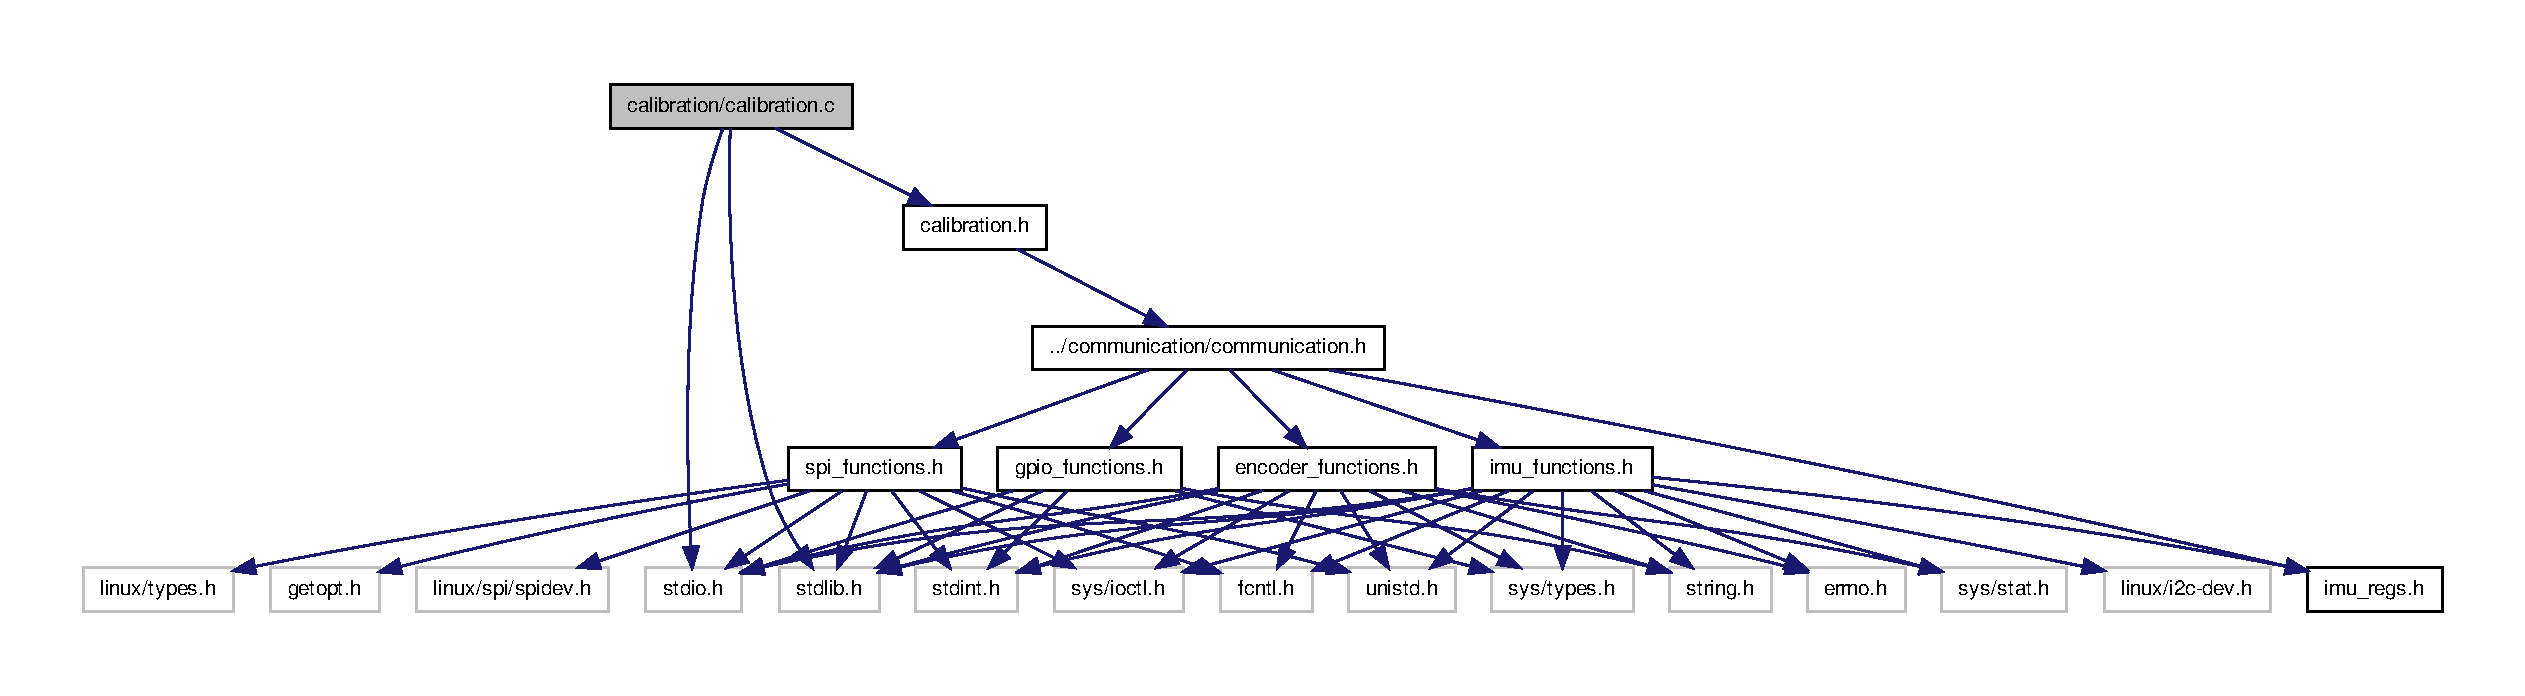
\includegraphics[width=350pt]{calibration_2calibration_8c__incl}
\end{center}
\end{figure}
\subsection*{Functions}
\begin{DoxyCompactItemize}
\item 
void \hyperlink{calibration_2calibration_8c_a043045246cf217758281222214c4addc}{calibrate\-\_\-all} (\hyperlink{structIMU__DATA__STRUCT}{I\-M\-U\-\_\-\-D\-A\-T\-A\-\_\-\-S\-T\-R\-U\-C\-T} $\ast$\hyperlink{threads__linux_8c_a3cfea12cbe9ca7f1681c950e4cd68606}{imu\-\_\-data})
\item 
void \hyperlink{calibration_2calibration_8c_aecfc81d152db2843b5d1517729804d63}{calibrate\-\_\-imu} (\hyperlink{structIMU__DATA__STRUCT}{I\-M\-U\-\_\-\-D\-A\-T\-A\-\_\-\-S\-T\-R\-U\-C\-T} $\ast$\hyperlink{threads__linux_8c_a3cfea12cbe9ca7f1681c950e4cd68606}{imu\-\_\-data})
\end{DoxyCompactItemize}


\subsection{Function Documentation}
\hypertarget{calibration_2calibration_8c_a043045246cf217758281222214c4addc}{\index{calibration/calibration.\-c@{calibration/calibration.\-c}!calibrate\-\_\-all@{calibrate\-\_\-all}}
\index{calibrate\-\_\-all@{calibrate\-\_\-all}!calibration/calibration.c@{calibration/calibration.\-c}}
\subsubsection[{calibrate\-\_\-all}]{\setlength{\rightskip}{0pt plus 5cm}void calibrate\-\_\-all (
\begin{DoxyParamCaption}
\item[{{\bf I\-M\-U\-\_\-\-D\-A\-T\-A\-\_\-\-S\-T\-R\-U\-C\-T} $\ast$}]{imu\-\_\-data}
\end{DoxyParamCaption}
)}}\label{calibration_2calibration_8c_a043045246cf217758281222214c4addc}


Definition at line 8 of file calibration.\-c.


\begin{DoxyCode}
\{
  \hyperlink{calibration_2calibration_8c_aecfc81d152db2843b5d1517729804d63}{calibrate\_imu}(imu\_data);
  \textcolor{keywordflow}{return};
\}
\end{DoxyCode}
\hypertarget{calibration_2calibration_8c_aecfc81d152db2843b5d1517729804d63}{\index{calibration/calibration.\-c@{calibration/calibration.\-c}!calibrate\-\_\-imu@{calibrate\-\_\-imu}}
\index{calibrate\-\_\-imu@{calibrate\-\_\-imu}!calibration/calibration.c@{calibration/calibration.\-c}}
\subsubsection[{calibrate\-\_\-imu}]{\setlength{\rightskip}{0pt plus 5cm}void calibrate\-\_\-imu (
\begin{DoxyParamCaption}
\item[{{\bf I\-M\-U\-\_\-\-D\-A\-T\-A\-\_\-\-S\-T\-R\-U\-C\-T} $\ast$}]{imu\-\_\-data}
\end{DoxyParamCaption}
)}}\label{calibration_2calibration_8c_aecfc81d152db2843b5d1517729804d63}


Definition at line 14 of file calibration.\-c.



Referenced by calibrate\-\_\-all().


\begin{DoxyCode}
\{
  \textcolor{comment}{// With this parameters, the vectors of acceleration and magnetic field will
       have norm = 1 theorically (i.e. in g or G)}
  imu\_data->\hyperlink{structIMU__DATA__STRUCT_aeffe3c3c5a7191a5cef16e7aab6c3795}{calib}.\hyperlink{structIMU__DATA__STRUCT_1_1calibrated_a281a7fdb40a05ed97388f18b9bb90c81}{acc}.\hyperlink{structDATA__XYZ__DOUBLE_a22868cc99a423900e7b82d015a5eb91f}{x} = ((double)imu\_data->\hyperlink{structIMU__DATA__STRUCT_a448f284bf44eb503affda586ad5fa9d2}{acc}.\hyperlink{structDATA__XYZ_a54c1596e9f9969fd9c21e8458024ecfb}{x}-\hyperlink{calibration_2calibration_8h_a355ea8f6ceed1e1d419a3ea2271bfca3}{ACC\_BIAS\_X}
      )/\hyperlink{calibration_2calibration_8h_a76e6967cb5a86ec34986b4583ac09831}{ACC\_FS\_X};
  imu\_data->\hyperlink{structIMU__DATA__STRUCT_aeffe3c3c5a7191a5cef16e7aab6c3795}{calib}.\hyperlink{structIMU__DATA__STRUCT_1_1calibrated_a281a7fdb40a05ed97388f18b9bb90c81}{acc}.\hyperlink{structDATA__XYZ__DOUBLE_a198a27b5df3b5b0bf461b0e481e22a82}{y} = ((double)imu\_data->\hyperlink{structIMU__DATA__STRUCT_a448f284bf44eb503affda586ad5fa9d2}{acc}.\hyperlink{structDATA__XYZ_a94bbb1c889bf53eb6a5fffa2b39322cf}{y}-\hyperlink{calibration_2calibration_8h_a34180f1c97e84a814ef181f62bf4b68f}{ACC\_BIAS\_Y}
      )/\hyperlink{calibration_2calibration_8h_a13d3aaab3b5800b11351cbd1246c8918}{ACC\_FS\_Y};
  imu\_data->\hyperlink{structIMU__DATA__STRUCT_aeffe3c3c5a7191a5cef16e7aab6c3795}{calib}.\hyperlink{structIMU__DATA__STRUCT_1_1calibrated_a281a7fdb40a05ed97388f18b9bb90c81}{acc}.\hyperlink{structDATA__XYZ__DOUBLE_a9556e8868c223ff3e28756ea18a284c0}{z} = ((double)imu\_data->\hyperlink{structIMU__DATA__STRUCT_a448f284bf44eb503affda586ad5fa9d2}{acc}.\hyperlink{structDATA__XYZ_a69e89ab0ec6e5d72fc5d54f62cc07fb5}{z}-\hyperlink{calibration_2calibration_8h_a794f762650b6f228ffb8d50d1323dbea}{ACC\_BIAS\_Z}
      )/\hyperlink{calibration_2calibration_8h_af1d3370cc0958289199c8c13470602d4}{ACC\_FS\_Z};
  
  imu\_data->\hyperlink{structIMU__DATA__STRUCT_aeffe3c3c5a7191a5cef16e7aab6c3795}{calib}.\hyperlink{structIMU__DATA__STRUCT_1_1calibrated_a2fde6c6759e0fda17e272c32096cb9ec}{mag}.\hyperlink{structDATA__XYZ__DOUBLE_a22868cc99a423900e7b82d015a5eb91f}{x} = ((double)imu\_data->\hyperlink{structIMU__DATA__STRUCT_a40c7df8b6d49297aa52873cfd9b60daa}{mag}.\hyperlink{structDATA__XYZ_a54c1596e9f9969fd9c21e8458024ecfb}{x}-\hyperlink{calibration_2calibration_8h_a355ea8f6ceed1e1d419a3ea2271bfca3}{ACC\_BIAS\_X}
      )/\hyperlink{calibration_2calibration_8h_a76e6967cb5a86ec34986b4583ac09831}{ACC\_FS\_X};
  imu\_data->\hyperlink{structIMU__DATA__STRUCT_aeffe3c3c5a7191a5cef16e7aab6c3795}{calib}.\hyperlink{structIMU__DATA__STRUCT_1_1calibrated_a2fde6c6759e0fda17e272c32096cb9ec}{mag}.\hyperlink{structDATA__XYZ__DOUBLE_a198a27b5df3b5b0bf461b0e481e22a82}{y} = ((double)imu\_data->\hyperlink{structIMU__DATA__STRUCT_a40c7df8b6d49297aa52873cfd9b60daa}{mag}.\hyperlink{structDATA__XYZ_a94bbb1c889bf53eb6a5fffa2b39322cf}{y}-\hyperlink{calibration_2calibration_8h_a34180f1c97e84a814ef181f62bf4b68f}{ACC\_BIAS\_Y}
      )/\hyperlink{calibration_2calibration_8h_a13d3aaab3b5800b11351cbd1246c8918}{ACC\_FS\_Y};
  imu\_data->\hyperlink{structIMU__DATA__STRUCT_aeffe3c3c5a7191a5cef16e7aab6c3795}{calib}.\hyperlink{structIMU__DATA__STRUCT_1_1calibrated_a2fde6c6759e0fda17e272c32096cb9ec}{mag}.\hyperlink{structDATA__XYZ__DOUBLE_a9556e8868c223ff3e28756ea18a284c0}{z} = ((double)imu\_data->\hyperlink{structIMU__DATA__STRUCT_a40c7df8b6d49297aa52873cfd9b60daa}{mag}.\hyperlink{structDATA__XYZ_a69e89ab0ec6e5d72fc5d54f62cc07fb5}{z}-\hyperlink{calibration_2calibration_8h_a794f762650b6f228ffb8d50d1323dbea}{ACC\_BIAS\_Z}
      )/\hyperlink{calibration_2calibration_8h_af1d3370cc0958289199c8c13470602d4}{ACC\_FS\_Z};
  
  \textcolor{comment}{// With this parameters, we consider right datasheet scale and we get in
       rad/s}
  imu\_data->\hyperlink{structIMU__DATA__STRUCT_aeffe3c3c5a7191a5cef16e7aab6c3795}{calib}.\hyperlink{structIMU__DATA__STRUCT_1_1calibrated_a8a54aded6ce608f1b7d2b4a0c52c248b}{gyr}.\hyperlink{structDATA__XYZ__DOUBLE_a22868cc99a423900e7b82d015a5eb91f}{x} = ((double)imu\_data->\hyperlink{structIMU__DATA__STRUCT_a0c1ac26626e4434a2ee124a1928a23a1}{gyr}.\hyperlink{structDATA__XYZ_a54c1596e9f9969fd9c21e8458024ecfb}{x}-\hyperlink{calibration_2calibration_8h_a69780ffe3a15aad4121fed56d5e47377}{GYR\_BIAS\_X}
      )/\hyperlink{calibration_2calibration_8h_a8fe84f8c6d39f41d8622fd0cbce3a522}{GYR\_FS\_X};
  imu\_data->\hyperlink{structIMU__DATA__STRUCT_aeffe3c3c5a7191a5cef16e7aab6c3795}{calib}.\hyperlink{structIMU__DATA__STRUCT_1_1calibrated_a8a54aded6ce608f1b7d2b4a0c52c248b}{gyr}.\hyperlink{structDATA__XYZ__DOUBLE_a198a27b5df3b5b0bf461b0e481e22a82}{y} = ((double)imu\_data->\hyperlink{structIMU__DATA__STRUCT_a0c1ac26626e4434a2ee124a1928a23a1}{gyr}.\hyperlink{structDATA__XYZ_a94bbb1c889bf53eb6a5fffa2b39322cf}{y}-\hyperlink{calibration_2calibration_8h_a69780ffe3a15aad4121fed56d5e47377}{GYR\_BIAS\_X}
      )/\hyperlink{calibration_2calibration_8h_a4be2e0fa7596546bb4699862d0fe4183}{GYR\_FS\_Y};
  imu\_data->\hyperlink{structIMU__DATA__STRUCT_aeffe3c3c5a7191a5cef16e7aab6c3795}{calib}.\hyperlink{structIMU__DATA__STRUCT_1_1calibrated_a8a54aded6ce608f1b7d2b4a0c52c248b}{gyr}.\hyperlink{structDATA__XYZ__DOUBLE_a9556e8868c223ff3e28756ea18a284c0}{z} = ((double)imu\_data->\hyperlink{structIMU__DATA__STRUCT_a0c1ac26626e4434a2ee124a1928a23a1}{gyr}.\hyperlink{structDATA__XYZ_a69e89ab0ec6e5d72fc5d54f62cc07fb5}{z}-\hyperlink{calibration_2calibration_8h_a69780ffe3a15aad4121fed56d5e47377}{GYR\_BIAS\_X}
      )/\hyperlink{calibration_2calibration_8h_aaee2ece0c43cc20d7c531ab79dcd06c8}{GYR\_FS\_Z};
  
  \textcolor{keywordflow}{return};
\}
\end{DoxyCode}


Here is the caller graph for this function\-:\nopagebreak
\begin{figure}[H]
\begin{center}
\leavevmode
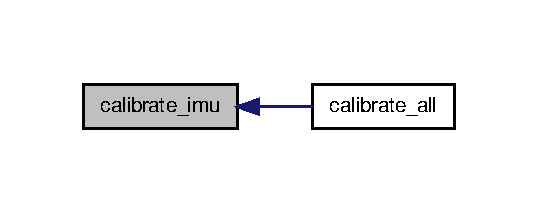
\includegraphics[width=258pt]{calibration_2calibration_8c_aecfc81d152db2843b5d1517729804d63_icgraph}
\end{center}
\end{figure}



\hypertarget{calibration_8c}{\section{calibration.\-c File Reference}
\label{calibration_8c}\index{calibration.\-c@{calibration.\-c}}
}
{\ttfamily \#include $<$stdio.\-h$>$}\\*
{\ttfamily \#include $<$stdlib.\-h$>$}\\*
{\ttfamily \#include \char`\"{}communication/communication.\-h\char`\"{}}\\*
{\ttfamily \#include \char`\"{}calibration.\-h\char`\"{}}\\*
Include dependency graph for calibration.\-c\-:
\nopagebreak
\begin{figure}[H]
\begin{center}
\leavevmode
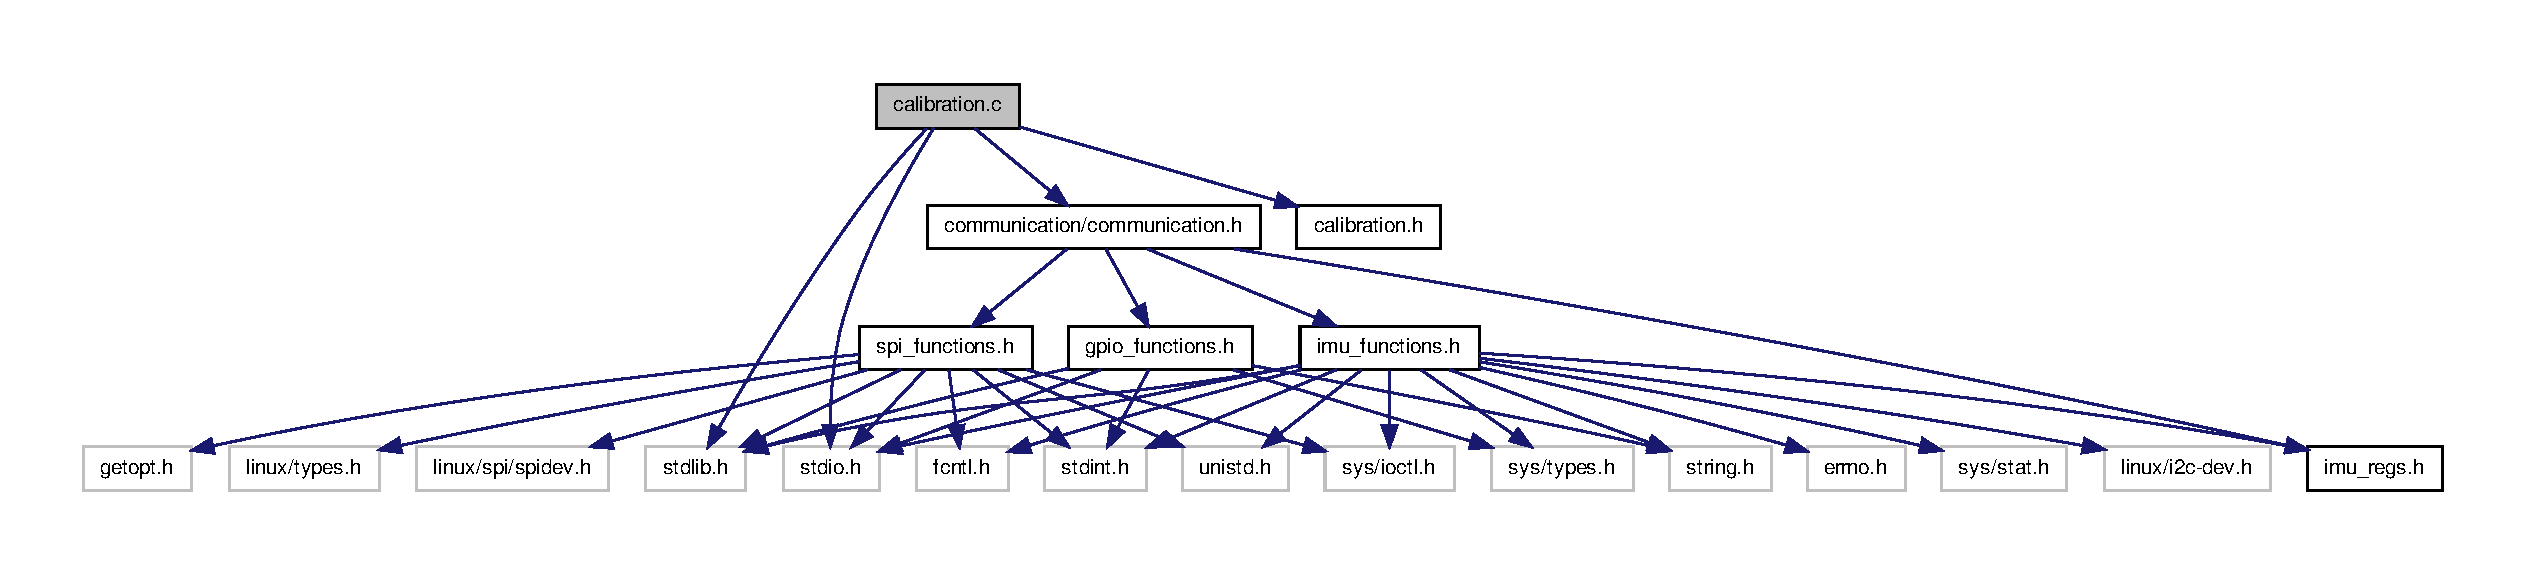
\includegraphics[width=350pt]{calibration_8c__incl}
\end{center}
\end{figure}
\subsection*{Functions}
\begin{DoxyCompactItemize}
\item 
void \hyperlink{group__calibrate_ga043045246cf217758281222214c4addc}{calibrate\-\_\-all} (\hyperlink{structIMU__DATA__STRUCT}{I\-M\-U\-\_\-\-D\-A\-T\-A\-\_\-\-S\-T\-R\-U\-C\-T} $\ast$\hyperlink{threads__linux_8c_a3cfea12cbe9ca7f1681c950e4cd68606}{imu\-\_\-data})
\begin{DoxyCompactList}\small\item\em Calibrate all sensors. \end{DoxyCompactList}\item 
void \hyperlink{group__calibrate_gaecfc81d152db2843b5d1517729804d63}{calibrate\-\_\-imu} (\hyperlink{structIMU__DATA__STRUCT}{I\-M\-U\-\_\-\-D\-A\-T\-A\-\_\-\-S\-T\-R\-U\-C\-T} $\ast$\hyperlink{threads__linux_8c_a3cfea12cbe9ca7f1681c950e4cd68606}{imu\-\_\-data})
\begin{DoxyCompactList}\small\item\em Calibrate imu sensors. \end{DoxyCompactList}\item 
void \hyperlink{calibration_8c_ae8f1281c6870b23c1c158b30998f7568}{calibrate\-\_\-enc} (\hyperlink{structENC__DATA__STRUCT}{E\-N\-C\-\_\-\-D\-A\-T\-A\-\_\-\-S\-T\-R\-U\-C\-T} $\ast$\hyperlink{main2_8c_aaa441e18ae805c4f3efb0b5231d1cfe7}{enc\-\_\-data})
\begin{DoxyCompactList}\small\item\em Calibrate encoder to return values in the rage of 0 to 90. \end{DoxyCompactList}\end{DoxyCompactItemize}


\subsection{Function Documentation}
\hypertarget{calibration_8c_ae8f1281c6870b23c1c158b30998f7568}{\index{calibration.\-c@{calibration.\-c}!calibrate\-\_\-enc@{calibrate\-\_\-enc}}
\index{calibrate\-\_\-enc@{calibrate\-\_\-enc}!calibration.c@{calibration.\-c}}
\subsubsection[{calibrate\-\_\-enc}]{\setlength{\rightskip}{0pt plus 5cm}void calibrate\-\_\-enc (
\begin{DoxyParamCaption}
\item[{{\bf E\-N\-C\-\_\-\-D\-A\-T\-A\-\_\-\-S\-T\-R\-U\-C\-T} $\ast$}]{enc\-\_\-data}
\end{DoxyParamCaption}
)}}\label{calibration_8c_ae8f1281c6870b23c1c158b30998f7568}


Calibrate encoder to return values in the rage of 0 to 90. 



Definition at line 35 of file calibration.\-c.



References E\-N\-C\-\_\-\-D\-A\-T\-A\-\_\-\-S\-T\-R\-U\-C\-T\-::calib, E\-N\-C\-\_\-\-F\-S, E\-N\-C\-\_\-\-M\-A\-X, E\-N\-C\-\_\-\-D\-A\-T\-A\-\_\-\-S\-T\-R\-U\-C\-T\-::position, and E\-N\-C\-\_\-\-D\-A\-T\-A\-\_\-\-S\-T\-R\-U\-C\-T\-::calibrate\-::position.


\begin{DoxyCode}
                                             \{
  enc\_data->\hyperlink{structENC__DATA__STRUCT_af227e5bbb714b830cc570432bda0a468}{calib}.\hyperlink{structENC__DATA__STRUCT_1_1calibrate_aed5100f7dc3d1f358a633c043e13cba2}{position} = ((\hyperlink{calibration_2calibration_8h_a496f1fb8343dc6e6bcdf07eb28557f41}{ENC\_MAX} - enc\_data->\hyperlink{structENC__DATA__STRUCT_ac3a53ed44ecaf87285518a091e1d2c24}{position}
      )/\hyperlink{calibration_2calibration_8h_adf9edcc7e266ed7333f7570965f5956a}{ENC\_FS});
\}
\end{DoxyCode}

\hypertarget{calibration_2calibration_8h}{\section{calibration/calibration.h File Reference}
\label{calibration_2calibration_8h}\index{calibration/calibration.\-h@{calibration/calibration.\-h}}
}
{\ttfamily \#include \char`\"{}../communication/communication.\-h\char`\"{}}\\*
\subsection*{Macros}
\begin{DoxyCompactItemize}
\item 
\#define \hyperlink{calibration_2calibration_8h_aa90cac659d18e8ef6294c7ae337f6b58}{S\-U\-C\-C\-E\-S\-S}~1
\item 
\#define \hyperlink{calibration_2calibration_8h_a6d58f9ac447476b4e084d7ca383f5183}{F\-A\-I\-L\-U\-R\-E}~-\/1
\item 
\#define \hyperlink{calibration_2calibration_8h_a355ea8f6ceed1e1d419a3ea2271bfca3}{A\-C\-C\-\_\-\-B\-I\-A\-S\-\_\-\-X}~19.\-2
\item 
\#define \hyperlink{calibration_2calibration_8h_a34180f1c97e84a814ef181f62bf4b68f}{A\-C\-C\-\_\-\-B\-I\-A\-S\-\_\-\-Y}~6.\-024
\item 
\#define \hyperlink{calibration_2calibration_8h_a794f762650b6f228ffb8d50d1323dbea}{A\-C\-C\-\_\-\-B\-I\-A\-S\-\_\-\-Z}~-\/18.\-97
\item 
\#define \hyperlink{calibration_2calibration_8h_a76e6967cb5a86ec34986b4583ac09831}{A\-C\-C\-\_\-\-F\-S\-\_\-\-X}~262.\-82
\item 
\#define \hyperlink{calibration_2calibration_8h_a13d3aaab3b5800b11351cbd1246c8918}{A\-C\-C\-\_\-\-F\-S\-\_\-\-Y}~262.\-15
\item 
\#define \hyperlink{calibration_2calibration_8h_af1d3370cc0958289199c8c13470602d4}{A\-C\-C\-\_\-\-F\-S\-\_\-\-Z}~252.\-20
\item 
\#define \hyperlink{calibration_2calibration_8h_a33f53b04fe0f887e8d9d99e4374c0ddf}{M\-A\-G\-\_\-\-B\-I\-A\-S\-\_\-\-X}~-\/143
\item 
\#define \hyperlink{calibration_2calibration_8h_a92407f4dfd1c63cede9a5307b379c569}{M\-A\-G\-\_\-\-B\-I\-A\-S\-\_\-\-Y}~-\/101
\item 
\#define \hyperlink{calibration_2calibration_8h_a9662c4fff54f93bcc4e043e84e79d623}{M\-A\-G\-\_\-\-B\-I\-A\-S\-\_\-\-Z}~3
\item 
\#define \hyperlink{calibration_2calibration_8h_aa49abc19ca0fda3324df06bddae2c1d4}{M\-A\-G\-\_\-\-F\-S\-\_\-\-X}~177
\item 
\#define \hyperlink{calibration_2calibration_8h_a5c5e64196104a5e5ebac3c594220eb5c}{M\-A\-G\-\_\-\-F\-S\-\_\-\-Y}~139
\item 
\#define \hyperlink{calibration_2calibration_8h_aebfc43ba340d89fa86b4a5c07cc7c924}{M\-A\-G\-\_\-\-F\-S\-\_\-\-Z}~85
\item 
\#define \hyperlink{calibration_2calibration_8h_a69780ffe3a15aad4121fed56d5e47377}{G\-Y\-R\-\_\-\-B\-I\-A\-S\-\_\-\-X}~-\/60.\-9046
\item 
\#define \hyperlink{calibration_2calibration_8h_af3264a08be995ea97ae8581128873877}{G\-Y\-R\-\_\-\-B\-I\-A\-S\-\_\-\-Y}~40.\-9062
\item 
\#define \hyperlink{calibration_2calibration_8h_aa10980bbf5b1dd91704d4dab98fcf991}{G\-Y\-R\-\_\-\-B\-I\-A\-S\-\_\-\-Z}~0.\-8769
\item 
\#define \hyperlink{calibration_2calibration_8h_a8fe84f8c6d39f41d8622fd0cbce3a522}{G\-Y\-R\-\_\-\-F\-S\-\_\-\-X}~0.\-001214142
\item 
\#define \hyperlink{calibration_2calibration_8h_a4be2e0fa7596546bb4699862d0fe4183}{G\-Y\-R\-\_\-\-F\-S\-\_\-\-Y}~0.\-001214142
\item 
\#define \hyperlink{calibration_2calibration_8h_aaee2ece0c43cc20d7c531ab79dcd06c8}{G\-Y\-R\-\_\-\-F\-S\-\_\-\-Z}~0.\-001214142
\end{DoxyCompactItemize}
\subsection*{Functions}
\begin{DoxyCompactItemize}
\item 
void \hyperlink{calibration_2calibration_8h_a043045246cf217758281222214c4addc}{calibrate\-\_\-all} (\hyperlink{structIMU__DATA__STRUCT}{I\-M\-U\-\_\-\-D\-A\-T\-A\-\_\-\-S\-T\-R\-U\-C\-T} $\ast$\hyperlink{threads__linux_8c_a3cfea12cbe9ca7f1681c950e4cd68606}{imu\-\_\-data})
\item 
void \hyperlink{calibration_2calibration_8h_aecfc81d152db2843b5d1517729804d63}{calibrate\-\_\-imu} (\hyperlink{structIMU__DATA__STRUCT}{I\-M\-U\-\_\-\-D\-A\-T\-A\-\_\-\-S\-T\-R\-U\-C\-T} $\ast$\hyperlink{threads__linux_8c_a3cfea12cbe9ca7f1681c950e4cd68606}{imu\-\_\-data})
\end{DoxyCompactItemize}


\subsection{Macro Definition Documentation}
\hypertarget{calibration_2calibration_8h_a355ea8f6ceed1e1d419a3ea2271bfca3}{\index{calibration/calibration.\-h@{calibration/calibration.\-h}!A\-C\-C\-\_\-\-B\-I\-A\-S\-\_\-\-X@{A\-C\-C\-\_\-\-B\-I\-A\-S\-\_\-\-X}}
\index{A\-C\-C\-\_\-\-B\-I\-A\-S\-\_\-\-X@{A\-C\-C\-\_\-\-B\-I\-A\-S\-\_\-\-X}!calibration/calibration.h@{calibration/calibration.\-h}}
\subsubsection[{A\-C\-C\-\_\-\-B\-I\-A\-S\-\_\-\-X}]{\setlength{\rightskip}{0pt plus 5cm}\#define A\-C\-C\-\_\-\-B\-I\-A\-S\-\_\-\-X~19.\-2}}\label{calibration_2calibration_8h_a355ea8f6ceed1e1d419a3ea2271bfca3}


Definition at line 10 of file calibration.\-h.



Referenced by calibrate\-\_\-imu().

\hypertarget{calibration_2calibration_8h_a34180f1c97e84a814ef181f62bf4b68f}{\index{calibration/calibration.\-h@{calibration/calibration.\-h}!A\-C\-C\-\_\-\-B\-I\-A\-S\-\_\-\-Y@{A\-C\-C\-\_\-\-B\-I\-A\-S\-\_\-\-Y}}
\index{A\-C\-C\-\_\-\-B\-I\-A\-S\-\_\-\-Y@{A\-C\-C\-\_\-\-B\-I\-A\-S\-\_\-\-Y}!calibration/calibration.h@{calibration/calibration.\-h}}
\subsubsection[{A\-C\-C\-\_\-\-B\-I\-A\-S\-\_\-\-Y}]{\setlength{\rightskip}{0pt plus 5cm}\#define A\-C\-C\-\_\-\-B\-I\-A\-S\-\_\-\-Y~6.\-024}}\label{calibration_2calibration_8h_a34180f1c97e84a814ef181f62bf4b68f}


Definition at line 11 of file calibration.\-h.



Referenced by calibrate\-\_\-imu().

\hypertarget{calibration_2calibration_8h_a794f762650b6f228ffb8d50d1323dbea}{\index{calibration/calibration.\-h@{calibration/calibration.\-h}!A\-C\-C\-\_\-\-B\-I\-A\-S\-\_\-\-Z@{A\-C\-C\-\_\-\-B\-I\-A\-S\-\_\-\-Z}}
\index{A\-C\-C\-\_\-\-B\-I\-A\-S\-\_\-\-Z@{A\-C\-C\-\_\-\-B\-I\-A\-S\-\_\-\-Z}!calibration/calibration.h@{calibration/calibration.\-h}}
\subsubsection[{A\-C\-C\-\_\-\-B\-I\-A\-S\-\_\-\-Z}]{\setlength{\rightskip}{0pt plus 5cm}\#define A\-C\-C\-\_\-\-B\-I\-A\-S\-\_\-\-Z~-\/18.\-97}}\label{calibration_2calibration_8h_a794f762650b6f228ffb8d50d1323dbea}


Definition at line 12 of file calibration.\-h.



Referenced by calibrate\-\_\-imu().

\hypertarget{calibration_2calibration_8h_a76e6967cb5a86ec34986b4583ac09831}{\index{calibration/calibration.\-h@{calibration/calibration.\-h}!A\-C\-C\-\_\-\-F\-S\-\_\-\-X@{A\-C\-C\-\_\-\-F\-S\-\_\-\-X}}
\index{A\-C\-C\-\_\-\-F\-S\-\_\-\-X@{A\-C\-C\-\_\-\-F\-S\-\_\-\-X}!calibration/calibration.h@{calibration/calibration.\-h}}
\subsubsection[{A\-C\-C\-\_\-\-F\-S\-\_\-\-X}]{\setlength{\rightskip}{0pt plus 5cm}\#define A\-C\-C\-\_\-\-F\-S\-\_\-\-X~262.\-82}}\label{calibration_2calibration_8h_a76e6967cb5a86ec34986b4583ac09831}


Definition at line 13 of file calibration.\-h.



Referenced by calibrate\-\_\-imu().

\hypertarget{calibration_2calibration_8h_a13d3aaab3b5800b11351cbd1246c8918}{\index{calibration/calibration.\-h@{calibration/calibration.\-h}!A\-C\-C\-\_\-\-F\-S\-\_\-\-Y@{A\-C\-C\-\_\-\-F\-S\-\_\-\-Y}}
\index{A\-C\-C\-\_\-\-F\-S\-\_\-\-Y@{A\-C\-C\-\_\-\-F\-S\-\_\-\-Y}!calibration/calibration.h@{calibration/calibration.\-h}}
\subsubsection[{A\-C\-C\-\_\-\-F\-S\-\_\-\-Y}]{\setlength{\rightskip}{0pt plus 5cm}\#define A\-C\-C\-\_\-\-F\-S\-\_\-\-Y~262.\-15}}\label{calibration_2calibration_8h_a13d3aaab3b5800b11351cbd1246c8918}


Definition at line 14 of file calibration.\-h.



Referenced by calibrate\-\_\-imu().

\hypertarget{calibration_2calibration_8h_af1d3370cc0958289199c8c13470602d4}{\index{calibration/calibration.\-h@{calibration/calibration.\-h}!A\-C\-C\-\_\-\-F\-S\-\_\-\-Z@{A\-C\-C\-\_\-\-F\-S\-\_\-\-Z}}
\index{A\-C\-C\-\_\-\-F\-S\-\_\-\-Z@{A\-C\-C\-\_\-\-F\-S\-\_\-\-Z}!calibration/calibration.h@{calibration/calibration.\-h}}
\subsubsection[{A\-C\-C\-\_\-\-F\-S\-\_\-\-Z}]{\setlength{\rightskip}{0pt plus 5cm}\#define A\-C\-C\-\_\-\-F\-S\-\_\-\-Z~252.\-20}}\label{calibration_2calibration_8h_af1d3370cc0958289199c8c13470602d4}


Definition at line 15 of file calibration.\-h.



Referenced by calibrate\-\_\-imu().

\hypertarget{calibration_2calibration_8h_a6d58f9ac447476b4e084d7ca383f5183}{\index{calibration/calibration.\-h@{calibration/calibration.\-h}!F\-A\-I\-L\-U\-R\-E@{F\-A\-I\-L\-U\-R\-E}}
\index{F\-A\-I\-L\-U\-R\-E@{F\-A\-I\-L\-U\-R\-E}!calibration/calibration.h@{calibration/calibration.\-h}}
\subsubsection[{F\-A\-I\-L\-U\-R\-E}]{\setlength{\rightskip}{0pt plus 5cm}\#define F\-A\-I\-L\-U\-R\-E~-\/1}}\label{calibration_2calibration_8h_a6d58f9ac447476b4e084d7ca383f5183}


Definition at line 7 of file calibration.\-h.



Referenced by acc\-\_\-init(), acc\-\_\-read\-\_\-all\-\_\-data(), acc\-\_\-write\-\_\-reg(), actuate(), devices\-\_\-init(), gpio\-\_\-read(), gpio\-\_\-write(), gyr\-\_\-read\-\_\-all\-\_\-data(), gyr\-\_\-write\-\_\-reg(), mag\-\_\-read\-\_\-all\-\_\-data(), main(), read\-\_\-all\-\_\-data(), and ui\-\_\-update().

\hypertarget{calibration_2calibration_8h_a69780ffe3a15aad4121fed56d5e47377}{\index{calibration/calibration.\-h@{calibration/calibration.\-h}!G\-Y\-R\-\_\-\-B\-I\-A\-S\-\_\-\-X@{G\-Y\-R\-\_\-\-B\-I\-A\-S\-\_\-\-X}}
\index{G\-Y\-R\-\_\-\-B\-I\-A\-S\-\_\-\-X@{G\-Y\-R\-\_\-\-B\-I\-A\-S\-\_\-\-X}!calibration/calibration.h@{calibration/calibration.\-h}}
\subsubsection[{G\-Y\-R\-\_\-\-B\-I\-A\-S\-\_\-\-X}]{\setlength{\rightskip}{0pt plus 5cm}\#define G\-Y\-R\-\_\-\-B\-I\-A\-S\-\_\-\-X~-\/60.\-9046}}\label{calibration_2calibration_8h_a69780ffe3a15aad4121fed56d5e47377}


Definition at line 25 of file calibration.\-h.



Referenced by calibrate\-\_\-imu().

\hypertarget{calibration_2calibration_8h_af3264a08be995ea97ae8581128873877}{\index{calibration/calibration.\-h@{calibration/calibration.\-h}!G\-Y\-R\-\_\-\-B\-I\-A\-S\-\_\-\-Y@{G\-Y\-R\-\_\-\-B\-I\-A\-S\-\_\-\-Y}}
\index{G\-Y\-R\-\_\-\-B\-I\-A\-S\-\_\-\-Y@{G\-Y\-R\-\_\-\-B\-I\-A\-S\-\_\-\-Y}!calibration/calibration.h@{calibration/calibration.\-h}}
\subsubsection[{G\-Y\-R\-\_\-\-B\-I\-A\-S\-\_\-\-Y}]{\setlength{\rightskip}{0pt plus 5cm}\#define G\-Y\-R\-\_\-\-B\-I\-A\-S\-\_\-\-Y~40.\-9062}}\label{calibration_2calibration_8h_af3264a08be995ea97ae8581128873877}


Definition at line 26 of file calibration.\-h.



Referenced by calibrate\-\_\-imu().

\hypertarget{calibration_2calibration_8h_aa10980bbf5b1dd91704d4dab98fcf991}{\index{calibration/calibration.\-h@{calibration/calibration.\-h}!G\-Y\-R\-\_\-\-B\-I\-A\-S\-\_\-\-Z@{G\-Y\-R\-\_\-\-B\-I\-A\-S\-\_\-\-Z}}
\index{G\-Y\-R\-\_\-\-B\-I\-A\-S\-\_\-\-Z@{G\-Y\-R\-\_\-\-B\-I\-A\-S\-\_\-\-Z}!calibration/calibration.h@{calibration/calibration.\-h}}
\subsubsection[{G\-Y\-R\-\_\-\-B\-I\-A\-S\-\_\-\-Z}]{\setlength{\rightskip}{0pt plus 5cm}\#define G\-Y\-R\-\_\-\-B\-I\-A\-S\-\_\-\-Z~0.\-8769}}\label{calibration_2calibration_8h_aa10980bbf5b1dd91704d4dab98fcf991}


Definition at line 27 of file calibration.\-h.



Referenced by calibrate\-\_\-imu().

\hypertarget{calibration_2calibration_8h_a8fe84f8c6d39f41d8622fd0cbce3a522}{\index{calibration/calibration.\-h@{calibration/calibration.\-h}!G\-Y\-R\-\_\-\-F\-S\-\_\-\-X@{G\-Y\-R\-\_\-\-F\-S\-\_\-\-X}}
\index{G\-Y\-R\-\_\-\-F\-S\-\_\-\-X@{G\-Y\-R\-\_\-\-F\-S\-\_\-\-X}!calibration/calibration.h@{calibration/calibration.\-h}}
\subsubsection[{G\-Y\-R\-\_\-\-F\-S\-\_\-\-X}]{\setlength{\rightskip}{0pt plus 5cm}\#define G\-Y\-R\-\_\-\-F\-S\-\_\-\-X~0.\-001214142}}\label{calibration_2calibration_8h_a8fe84f8c6d39f41d8622fd0cbce3a522}


Definition at line 28 of file calibration.\-h.



Referenced by calibrate\-\_\-imu().

\hypertarget{calibration_2calibration_8h_a4be2e0fa7596546bb4699862d0fe4183}{\index{calibration/calibration.\-h@{calibration/calibration.\-h}!G\-Y\-R\-\_\-\-F\-S\-\_\-\-Y@{G\-Y\-R\-\_\-\-F\-S\-\_\-\-Y}}
\index{G\-Y\-R\-\_\-\-F\-S\-\_\-\-Y@{G\-Y\-R\-\_\-\-F\-S\-\_\-\-Y}!calibration/calibration.h@{calibration/calibration.\-h}}
\subsubsection[{G\-Y\-R\-\_\-\-F\-S\-\_\-\-Y}]{\setlength{\rightskip}{0pt plus 5cm}\#define G\-Y\-R\-\_\-\-F\-S\-\_\-\-Y~0.\-001214142}}\label{calibration_2calibration_8h_a4be2e0fa7596546bb4699862d0fe4183}


Definition at line 29 of file calibration.\-h.



Referenced by calibrate\-\_\-imu().

\hypertarget{calibration_2calibration_8h_aaee2ece0c43cc20d7c531ab79dcd06c8}{\index{calibration/calibration.\-h@{calibration/calibration.\-h}!G\-Y\-R\-\_\-\-F\-S\-\_\-\-Z@{G\-Y\-R\-\_\-\-F\-S\-\_\-\-Z}}
\index{G\-Y\-R\-\_\-\-F\-S\-\_\-\-Z@{G\-Y\-R\-\_\-\-F\-S\-\_\-\-Z}!calibration/calibration.h@{calibration/calibration.\-h}}
\subsubsection[{G\-Y\-R\-\_\-\-F\-S\-\_\-\-Z}]{\setlength{\rightskip}{0pt plus 5cm}\#define G\-Y\-R\-\_\-\-F\-S\-\_\-\-Z~0.\-001214142}}\label{calibration_2calibration_8h_aaee2ece0c43cc20d7c531ab79dcd06c8}


Definition at line 30 of file calibration.\-h.



Referenced by calibrate\-\_\-imu().

\hypertarget{calibration_2calibration_8h_a33f53b04fe0f887e8d9d99e4374c0ddf}{\index{calibration/calibration.\-h@{calibration/calibration.\-h}!M\-A\-G\-\_\-\-B\-I\-A\-S\-\_\-\-X@{M\-A\-G\-\_\-\-B\-I\-A\-S\-\_\-\-X}}
\index{M\-A\-G\-\_\-\-B\-I\-A\-S\-\_\-\-X@{M\-A\-G\-\_\-\-B\-I\-A\-S\-\_\-\-X}!calibration/calibration.h@{calibration/calibration.\-h}}
\subsubsection[{M\-A\-G\-\_\-\-B\-I\-A\-S\-\_\-\-X}]{\setlength{\rightskip}{0pt plus 5cm}\#define M\-A\-G\-\_\-\-B\-I\-A\-S\-\_\-\-X~-\/143}}\label{calibration_2calibration_8h_a33f53b04fe0f887e8d9d99e4374c0ddf}


Definition at line 17 of file calibration.\-h.



Referenced by calibrate\-\_\-imu().

\hypertarget{calibration_2calibration_8h_a92407f4dfd1c63cede9a5307b379c569}{\index{calibration/calibration.\-h@{calibration/calibration.\-h}!M\-A\-G\-\_\-\-B\-I\-A\-S\-\_\-\-Y@{M\-A\-G\-\_\-\-B\-I\-A\-S\-\_\-\-Y}}
\index{M\-A\-G\-\_\-\-B\-I\-A\-S\-\_\-\-Y@{M\-A\-G\-\_\-\-B\-I\-A\-S\-\_\-\-Y}!calibration/calibration.h@{calibration/calibration.\-h}}
\subsubsection[{M\-A\-G\-\_\-\-B\-I\-A\-S\-\_\-\-Y}]{\setlength{\rightskip}{0pt plus 5cm}\#define M\-A\-G\-\_\-\-B\-I\-A\-S\-\_\-\-Y~-\/101}}\label{calibration_2calibration_8h_a92407f4dfd1c63cede9a5307b379c569}


Definition at line 18 of file calibration.\-h.



Referenced by calibrate\-\_\-imu().

\hypertarget{calibration_2calibration_8h_a9662c4fff54f93bcc4e043e84e79d623}{\index{calibration/calibration.\-h@{calibration/calibration.\-h}!M\-A\-G\-\_\-\-B\-I\-A\-S\-\_\-\-Z@{M\-A\-G\-\_\-\-B\-I\-A\-S\-\_\-\-Z}}
\index{M\-A\-G\-\_\-\-B\-I\-A\-S\-\_\-\-Z@{M\-A\-G\-\_\-\-B\-I\-A\-S\-\_\-\-Z}!calibration/calibration.h@{calibration/calibration.\-h}}
\subsubsection[{M\-A\-G\-\_\-\-B\-I\-A\-S\-\_\-\-Z}]{\setlength{\rightskip}{0pt plus 5cm}\#define M\-A\-G\-\_\-\-B\-I\-A\-S\-\_\-\-Z~3}}\label{calibration_2calibration_8h_a9662c4fff54f93bcc4e043e84e79d623}


Definition at line 19 of file calibration.\-h.



Referenced by calibrate\-\_\-imu().

\hypertarget{calibration_2calibration_8h_aa49abc19ca0fda3324df06bddae2c1d4}{\index{calibration/calibration.\-h@{calibration/calibration.\-h}!M\-A\-G\-\_\-\-F\-S\-\_\-\-X@{M\-A\-G\-\_\-\-F\-S\-\_\-\-X}}
\index{M\-A\-G\-\_\-\-F\-S\-\_\-\-X@{M\-A\-G\-\_\-\-F\-S\-\_\-\-X}!calibration/calibration.h@{calibration/calibration.\-h}}
\subsubsection[{M\-A\-G\-\_\-\-F\-S\-\_\-\-X}]{\setlength{\rightskip}{0pt plus 5cm}\#define M\-A\-G\-\_\-\-F\-S\-\_\-\-X~177}}\label{calibration_2calibration_8h_aa49abc19ca0fda3324df06bddae2c1d4}


Definition at line 20 of file calibration.\-h.



Referenced by calibrate\-\_\-imu().

\hypertarget{calibration_2calibration_8h_a5c5e64196104a5e5ebac3c594220eb5c}{\index{calibration/calibration.\-h@{calibration/calibration.\-h}!M\-A\-G\-\_\-\-F\-S\-\_\-\-Y@{M\-A\-G\-\_\-\-F\-S\-\_\-\-Y}}
\index{M\-A\-G\-\_\-\-F\-S\-\_\-\-Y@{M\-A\-G\-\_\-\-F\-S\-\_\-\-Y}!calibration/calibration.h@{calibration/calibration.\-h}}
\subsubsection[{M\-A\-G\-\_\-\-F\-S\-\_\-\-Y}]{\setlength{\rightskip}{0pt plus 5cm}\#define M\-A\-G\-\_\-\-F\-S\-\_\-\-Y~139}}\label{calibration_2calibration_8h_a5c5e64196104a5e5ebac3c594220eb5c}


Definition at line 21 of file calibration.\-h.



Referenced by calibrate\-\_\-imu().

\hypertarget{calibration_2calibration_8h_aebfc43ba340d89fa86b4a5c07cc7c924}{\index{calibration/calibration.\-h@{calibration/calibration.\-h}!M\-A\-G\-\_\-\-F\-S\-\_\-\-Z@{M\-A\-G\-\_\-\-F\-S\-\_\-\-Z}}
\index{M\-A\-G\-\_\-\-F\-S\-\_\-\-Z@{M\-A\-G\-\_\-\-F\-S\-\_\-\-Z}!calibration/calibration.h@{calibration/calibration.\-h}}
\subsubsection[{M\-A\-G\-\_\-\-F\-S\-\_\-\-Z}]{\setlength{\rightskip}{0pt plus 5cm}\#define M\-A\-G\-\_\-\-F\-S\-\_\-\-Z~85}}\label{calibration_2calibration_8h_aebfc43ba340d89fa86b4a5c07cc7c924}


Definition at line 22 of file calibration.\-h.



Referenced by calibrate\-\_\-imu().

\hypertarget{calibration_2calibration_8h_aa90cac659d18e8ef6294c7ae337f6b58}{\index{calibration/calibration.\-h@{calibration/calibration.\-h}!S\-U\-C\-C\-E\-S\-S@{S\-U\-C\-C\-E\-S\-S}}
\index{S\-U\-C\-C\-E\-S\-S@{S\-U\-C\-C\-E\-S\-S}!calibration/calibration.h@{calibration/calibration.\-h}}
\subsubsection[{S\-U\-C\-C\-E\-S\-S}]{\setlength{\rightskip}{0pt plus 5cm}\#define S\-U\-C\-C\-E\-S\-S~1}}\label{calibration_2calibration_8h_aa90cac659d18e8ef6294c7ae337f6b58}


Definition at line 6 of file calibration.\-h.



Referenced by acc\-\_\-init(), acc\-\_\-read\-\_\-all\-\_\-data(), acc\-\_\-write\-\_\-reg(), actuate(), devices\-\_\-init(), get\-\_\-time(), gpio\-\_\-f\-\_\-write(), gpio\-\_\-write(), gyr\-\_\-read\-\_\-all\-\_\-data(), mag\-\_\-read\-\_\-all\-\_\-data(), main(), periodic\-\_\-task\-\_\-1(), periodic\-\_\-task\-\_\-2(), read\-\_\-all\-\_\-data(), reset\-\_\-timer(), ui\-\_\-close(), ui\-\_\-eff\-\_\-data(), ui\-\_\-imu\-\_\-data(), ui\-\_\-init(), ui\-\_\-mra\-\_\-data(), ui\-\_\-overview\-\_\-data(), and ui\-\_\-update().



\subsection{Function Documentation}
\hypertarget{calibration_2calibration_8h_a043045246cf217758281222214c4addc}{\index{calibration/calibration.\-h@{calibration/calibration.\-h}!calibrate\-\_\-all@{calibrate\-\_\-all}}
\index{calibrate\-\_\-all@{calibrate\-\_\-all}!calibration/calibration.h@{calibration/calibration.\-h}}
\subsubsection[{calibrate\-\_\-all}]{\setlength{\rightskip}{0pt plus 5cm}void calibrate\-\_\-all (
\begin{DoxyParamCaption}
\item[{{\bf I\-M\-U\-\_\-\-D\-A\-T\-A\-\_\-\-S\-T\-R\-U\-C\-T} $\ast$}]{imu\-\_\-data}
\end{DoxyParamCaption}
)}}\label{calibration_2calibration_8h_a043045246cf217758281222214c4addc}


Definition at line 8 of file calibration.\-c.


\begin{DoxyCode}
\{
  \hyperlink{calibration_2calibration_8c_aecfc81d152db2843b5d1517729804d63}{calibrate\_imu}(imu\_data);
  \textcolor{keywordflow}{return};
\}
\end{DoxyCode}
\hypertarget{calibration_2calibration_8h_aecfc81d152db2843b5d1517729804d63}{\index{calibration/calibration.\-h@{calibration/calibration.\-h}!calibrate\-\_\-imu@{calibrate\-\_\-imu}}
\index{calibrate\-\_\-imu@{calibrate\-\_\-imu}!calibration/calibration.h@{calibration/calibration.\-h}}
\subsubsection[{calibrate\-\_\-imu}]{\setlength{\rightskip}{0pt plus 5cm}void calibrate\-\_\-imu (
\begin{DoxyParamCaption}
\item[{{\bf I\-M\-U\-\_\-\-D\-A\-T\-A\-\_\-\-S\-T\-R\-U\-C\-T} $\ast$}]{imu\-\_\-data}
\end{DoxyParamCaption}
)}}\label{calibration_2calibration_8h_aecfc81d152db2843b5d1517729804d63}


Definition at line 14 of file calibration.\-c.


\begin{DoxyCode}
\{
  \textcolor{comment}{// With this parameters, the vectors of acceleration and magnetic field will
       have norm = 1 theorically (i.e. in g or G)}
  imu\_data->\hyperlink{structIMU__DATA__STRUCT_aeffe3c3c5a7191a5cef16e7aab6c3795}{calib}.\hyperlink{structIMU__DATA__STRUCT_1_1calibrated_a281a7fdb40a05ed97388f18b9bb90c81}{acc}.\hyperlink{structDATA__XYZ__DOUBLE_a22868cc99a423900e7b82d015a5eb91f}{x} = ((double)imu\_data->\hyperlink{structIMU__DATA__STRUCT_a448f284bf44eb503affda586ad5fa9d2}{acc}.\hyperlink{structDATA__XYZ_a54c1596e9f9969fd9c21e8458024ecfb}{x}-\hyperlink{calibration_2calibration_8h_a355ea8f6ceed1e1d419a3ea2271bfca3}{ACC\_BIAS\_X}
      )/\hyperlink{calibration_2calibration_8h_a76e6967cb5a86ec34986b4583ac09831}{ACC\_FS\_X};
  imu\_data->\hyperlink{structIMU__DATA__STRUCT_aeffe3c3c5a7191a5cef16e7aab6c3795}{calib}.\hyperlink{structIMU__DATA__STRUCT_1_1calibrated_a281a7fdb40a05ed97388f18b9bb90c81}{acc}.\hyperlink{structDATA__XYZ__DOUBLE_a198a27b5df3b5b0bf461b0e481e22a82}{y} = ((double)imu\_data->\hyperlink{structIMU__DATA__STRUCT_a448f284bf44eb503affda586ad5fa9d2}{acc}.\hyperlink{structDATA__XYZ_a94bbb1c889bf53eb6a5fffa2b39322cf}{y}-\hyperlink{calibration_2calibration_8h_a34180f1c97e84a814ef181f62bf4b68f}{ACC\_BIAS\_Y}
      )/\hyperlink{calibration_2calibration_8h_a13d3aaab3b5800b11351cbd1246c8918}{ACC\_FS\_Y};
  imu\_data->\hyperlink{structIMU__DATA__STRUCT_aeffe3c3c5a7191a5cef16e7aab6c3795}{calib}.\hyperlink{structIMU__DATA__STRUCT_1_1calibrated_a281a7fdb40a05ed97388f18b9bb90c81}{acc}.\hyperlink{structDATA__XYZ__DOUBLE_a9556e8868c223ff3e28756ea18a284c0}{z} = ((double)imu\_data->\hyperlink{structIMU__DATA__STRUCT_a448f284bf44eb503affda586ad5fa9d2}{acc}.\hyperlink{structDATA__XYZ_a69e89ab0ec6e5d72fc5d54f62cc07fb5}{z}-\hyperlink{calibration_2calibration_8h_a794f762650b6f228ffb8d50d1323dbea}{ACC\_BIAS\_Z}
      )/\hyperlink{calibration_2calibration_8h_af1d3370cc0958289199c8c13470602d4}{ACC\_FS\_Z};
  
  imu\_data->\hyperlink{structIMU__DATA__STRUCT_aeffe3c3c5a7191a5cef16e7aab6c3795}{calib}.\hyperlink{structIMU__DATA__STRUCT_1_1calibrated_a2fde6c6759e0fda17e272c32096cb9ec}{mag}.\hyperlink{structDATA__XYZ__DOUBLE_a22868cc99a423900e7b82d015a5eb91f}{x} = ((double)imu\_data->\hyperlink{structIMU__DATA__STRUCT_a40c7df8b6d49297aa52873cfd9b60daa}{mag}.\hyperlink{structDATA__XYZ_a54c1596e9f9969fd9c21e8458024ecfb}{x}-\hyperlink{calibration_2calibration_8h_a355ea8f6ceed1e1d419a3ea2271bfca3}{ACC\_BIAS\_X}
      )/\hyperlink{calibration_2calibration_8h_a76e6967cb5a86ec34986b4583ac09831}{ACC\_FS\_X};
  imu\_data->\hyperlink{structIMU__DATA__STRUCT_aeffe3c3c5a7191a5cef16e7aab6c3795}{calib}.\hyperlink{structIMU__DATA__STRUCT_1_1calibrated_a2fde6c6759e0fda17e272c32096cb9ec}{mag}.\hyperlink{structDATA__XYZ__DOUBLE_a198a27b5df3b5b0bf461b0e481e22a82}{y} = ((double)imu\_data->\hyperlink{structIMU__DATA__STRUCT_a40c7df8b6d49297aa52873cfd9b60daa}{mag}.\hyperlink{structDATA__XYZ_a94bbb1c889bf53eb6a5fffa2b39322cf}{y}-\hyperlink{calibration_2calibration_8h_a34180f1c97e84a814ef181f62bf4b68f}{ACC\_BIAS\_Y}
      )/\hyperlink{calibration_2calibration_8h_a13d3aaab3b5800b11351cbd1246c8918}{ACC\_FS\_Y};
  imu\_data->\hyperlink{structIMU__DATA__STRUCT_aeffe3c3c5a7191a5cef16e7aab6c3795}{calib}.\hyperlink{structIMU__DATA__STRUCT_1_1calibrated_a2fde6c6759e0fda17e272c32096cb9ec}{mag}.\hyperlink{structDATA__XYZ__DOUBLE_a9556e8868c223ff3e28756ea18a284c0}{z} = ((double)imu\_data->\hyperlink{structIMU__DATA__STRUCT_a40c7df8b6d49297aa52873cfd9b60daa}{mag}.\hyperlink{structDATA__XYZ_a69e89ab0ec6e5d72fc5d54f62cc07fb5}{z}-\hyperlink{calibration_2calibration_8h_a794f762650b6f228ffb8d50d1323dbea}{ACC\_BIAS\_Z}
      )/\hyperlink{calibration_2calibration_8h_af1d3370cc0958289199c8c13470602d4}{ACC\_FS\_Z};
  
  \textcolor{comment}{// With this parameters, we consider right datasheet scale and we get in
       rad/s}
  imu\_data->\hyperlink{structIMU__DATA__STRUCT_aeffe3c3c5a7191a5cef16e7aab6c3795}{calib}.\hyperlink{structIMU__DATA__STRUCT_1_1calibrated_a8a54aded6ce608f1b7d2b4a0c52c248b}{gyr}.\hyperlink{structDATA__XYZ__DOUBLE_a22868cc99a423900e7b82d015a5eb91f}{x} = ((double)imu\_data->\hyperlink{structIMU__DATA__STRUCT_a0c1ac26626e4434a2ee124a1928a23a1}{gyr}.\hyperlink{structDATA__XYZ_a54c1596e9f9969fd9c21e8458024ecfb}{x}-\hyperlink{calibration_2calibration_8h_a69780ffe3a15aad4121fed56d5e47377}{GYR\_BIAS\_X}
      )/\hyperlink{calibration_2calibration_8h_a8fe84f8c6d39f41d8622fd0cbce3a522}{GYR\_FS\_X};
  imu\_data->\hyperlink{structIMU__DATA__STRUCT_aeffe3c3c5a7191a5cef16e7aab6c3795}{calib}.\hyperlink{structIMU__DATA__STRUCT_1_1calibrated_a8a54aded6ce608f1b7d2b4a0c52c248b}{gyr}.\hyperlink{structDATA__XYZ__DOUBLE_a198a27b5df3b5b0bf461b0e481e22a82}{y} = ((double)imu\_data->\hyperlink{structIMU__DATA__STRUCT_a0c1ac26626e4434a2ee124a1928a23a1}{gyr}.\hyperlink{structDATA__XYZ_a94bbb1c889bf53eb6a5fffa2b39322cf}{y}-\hyperlink{calibration_2calibration_8h_a69780ffe3a15aad4121fed56d5e47377}{GYR\_BIAS\_X}
      )/\hyperlink{calibration_2calibration_8h_a4be2e0fa7596546bb4699862d0fe4183}{GYR\_FS\_Y};
  imu\_data->\hyperlink{structIMU__DATA__STRUCT_aeffe3c3c5a7191a5cef16e7aab6c3795}{calib}.\hyperlink{structIMU__DATA__STRUCT_1_1calibrated_a8a54aded6ce608f1b7d2b4a0c52c248b}{gyr}.\hyperlink{structDATA__XYZ__DOUBLE_a9556e8868c223ff3e28756ea18a284c0}{z} = ((double)imu\_data->\hyperlink{structIMU__DATA__STRUCT_a0c1ac26626e4434a2ee124a1928a23a1}{gyr}.\hyperlink{structDATA__XYZ_a69e89ab0ec6e5d72fc5d54f62cc07fb5}{z}-\hyperlink{calibration_2calibration_8h_a69780ffe3a15aad4121fed56d5e47377}{GYR\_BIAS\_X}
      )/\hyperlink{calibration_2calibration_8h_aaee2ece0c43cc20d7c531ab79dcd06c8}{GYR\_FS\_Z};
  
  \textcolor{keywordflow}{return};
\}
\end{DoxyCode}

\hypertarget{calibration_8h}{\section{calibration.\-h File Reference}
\label{calibration_8h}\index{calibration.\-h@{calibration.\-h}}
}
This graph shows which files directly or indirectly include this file\-:\nopagebreak
\begin{figure}[H]
\begin{center}
\leavevmode
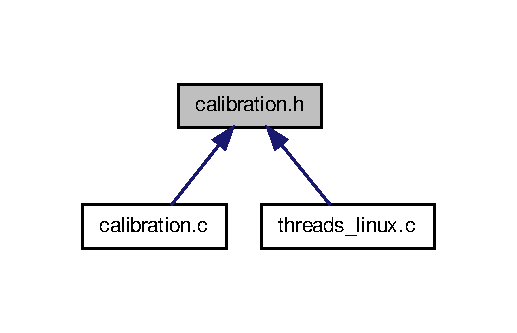
\includegraphics[width=248pt]{calibration_8h__dep__incl}
\end{center}
\end{figure}
\subsection*{Macros}
\begin{DoxyCompactItemize}
\item 
\#define \hyperlink{calibration_8h_aa90cac659d18e8ef6294c7ae337f6b58}{S\-U\-C\-C\-E\-S\-S}~1
\item 
\#define \hyperlink{calibration_8h_a6d58f9ac447476b4e084d7ca383f5183}{F\-A\-I\-L\-U\-R\-E}~-\/1
\item 
\#define \hyperlink{calibration_8h_a355ea8f6ceed1e1d419a3ea2271bfca3}{A\-C\-C\-\_\-\-B\-I\-A\-S\-\_\-\-X}~19.\-2
\item 
\#define \hyperlink{calibration_8h_a34180f1c97e84a814ef181f62bf4b68f}{A\-C\-C\-\_\-\-B\-I\-A\-S\-\_\-\-Y}~6.\-024
\item 
\#define \hyperlink{calibration_8h_a794f762650b6f228ffb8d50d1323dbea}{A\-C\-C\-\_\-\-B\-I\-A\-S\-\_\-\-Z}~-\/18.\-97
\item 
\#define \hyperlink{calibration_8h_a76e6967cb5a86ec34986b4583ac09831}{A\-C\-C\-\_\-\-F\-S\-\_\-\-X}~262.\-82
\item 
\#define \hyperlink{calibration_8h_a13d3aaab3b5800b11351cbd1246c8918}{A\-C\-C\-\_\-\-F\-S\-\_\-\-Y}~262.\-15
\item 
\#define \hyperlink{calibration_8h_af1d3370cc0958289199c8c13470602d4}{A\-C\-C\-\_\-\-F\-S\-\_\-\-Z}~252.\-20
\item 
\#define \hyperlink{calibration_8h_a33f53b04fe0f887e8d9d99e4374c0ddf}{M\-A\-G\-\_\-\-B\-I\-A\-S\-\_\-\-X}~-\/143
\item 
\#define \hyperlink{calibration_8h_a92407f4dfd1c63cede9a5307b379c569}{M\-A\-G\-\_\-\-B\-I\-A\-S\-\_\-\-Y}~-\/101
\item 
\#define \hyperlink{calibration_8h_a9662c4fff54f93bcc4e043e84e79d623}{M\-A\-G\-\_\-\-B\-I\-A\-S\-\_\-\-Z}~3
\item 
\#define \hyperlink{calibration_8h_aa49abc19ca0fda3324df06bddae2c1d4}{M\-A\-G\-\_\-\-F\-S\-\_\-\-X}~177
\item 
\#define \hyperlink{calibration_8h_a5c5e64196104a5e5ebac3c594220eb5c}{M\-A\-G\-\_\-\-F\-S\-\_\-\-Y}~139
\item 
\#define \hyperlink{calibration_8h_aebfc43ba340d89fa86b4a5c07cc7c924}{M\-A\-G\-\_\-\-F\-S\-\_\-\-Z}~85
\item 
\#define \hyperlink{calibration_8h_a69780ffe3a15aad4121fed56d5e47377}{G\-Y\-R\-\_\-\-B\-I\-A\-S\-\_\-\-X}~-\/60.\-8067
\item 
\#define \hyperlink{calibration_8h_af3264a08be995ea97ae8581128873877}{G\-Y\-R\-\_\-\-B\-I\-A\-S\-\_\-\-Y}~40.\-0800
\item 
\#define \hyperlink{calibration_8h_aa10980bbf5b1dd91704d4dab98fcf991}{G\-Y\-R\-\_\-\-B\-I\-A\-S\-\_\-\-Z}~0.\-7267
\item 
\#define \hyperlink{calibration_8h_a8fe84f8c6d39f41d8622fd0cbce3a522}{G\-Y\-R\-\_\-\-F\-S\-\_\-\-X}~0.\-001214142
\item 
\#define \hyperlink{calibration_8h_a4be2e0fa7596546bb4699862d0fe4183}{G\-Y\-R\-\_\-\-F\-S\-\_\-\-Y}~0.\-001214142
\item 
\#define \hyperlink{calibration_8h_aaee2ece0c43cc20d7c531ab79dcd06c8}{G\-Y\-R\-\_\-\-F\-S\-\_\-\-Z}~0.\-001214142
\end{DoxyCompactItemize}
\subsection*{Functions}
\begin{DoxyCompactItemize}
\item 
void \hyperlink{calibration_8h_a043045246cf217758281222214c4addc}{calibrate\-\_\-all} (\hyperlink{structIMU__DATA__STRUCT}{I\-M\-U\-\_\-\-D\-A\-T\-A\-\_\-\-S\-T\-R\-U\-C\-T} $\ast$\hyperlink{threads__linux_8c_a3cfea12cbe9ca7f1681c950e4cd68606}{imu\-\_\-data})
\item 
void \hyperlink{calibration_8h_aecfc81d152db2843b5d1517729804d63}{calibrate\-\_\-imu} (\hyperlink{structIMU__DATA__STRUCT}{I\-M\-U\-\_\-\-D\-A\-T\-A\-\_\-\-S\-T\-R\-U\-C\-T} $\ast$\hyperlink{threads__linux_8c_a3cfea12cbe9ca7f1681c950e4cd68606}{imu\-\_\-data})
\end{DoxyCompactItemize}


\subsection{Macro Definition Documentation}
\hypertarget{calibration_8h_a355ea8f6ceed1e1d419a3ea2271bfca3}{\index{calibration.\-h@{calibration.\-h}!A\-C\-C\-\_\-\-B\-I\-A\-S\-\_\-\-X@{A\-C\-C\-\_\-\-B\-I\-A\-S\-\_\-\-X}}
\index{A\-C\-C\-\_\-\-B\-I\-A\-S\-\_\-\-X@{A\-C\-C\-\_\-\-B\-I\-A\-S\-\_\-\-X}!calibration.h@{calibration.\-h}}
\subsubsection[{A\-C\-C\-\_\-\-B\-I\-A\-S\-\_\-\-X}]{\setlength{\rightskip}{0pt plus 5cm}\#define A\-C\-C\-\_\-\-B\-I\-A\-S\-\_\-\-X~19.\-2}}\label{calibration_8h_a355ea8f6ceed1e1d419a3ea2271bfca3}


Definition at line 10 of file calibration.\-h.

\hypertarget{calibration_8h_a34180f1c97e84a814ef181f62bf4b68f}{\index{calibration.\-h@{calibration.\-h}!A\-C\-C\-\_\-\-B\-I\-A\-S\-\_\-\-Y@{A\-C\-C\-\_\-\-B\-I\-A\-S\-\_\-\-Y}}
\index{A\-C\-C\-\_\-\-B\-I\-A\-S\-\_\-\-Y@{A\-C\-C\-\_\-\-B\-I\-A\-S\-\_\-\-Y}!calibration.h@{calibration.\-h}}
\subsubsection[{A\-C\-C\-\_\-\-B\-I\-A\-S\-\_\-\-Y}]{\setlength{\rightskip}{0pt plus 5cm}\#define A\-C\-C\-\_\-\-B\-I\-A\-S\-\_\-\-Y~6.\-024}}\label{calibration_8h_a34180f1c97e84a814ef181f62bf4b68f}


Definition at line 11 of file calibration.\-h.

\hypertarget{calibration_8h_a794f762650b6f228ffb8d50d1323dbea}{\index{calibration.\-h@{calibration.\-h}!A\-C\-C\-\_\-\-B\-I\-A\-S\-\_\-\-Z@{A\-C\-C\-\_\-\-B\-I\-A\-S\-\_\-\-Z}}
\index{A\-C\-C\-\_\-\-B\-I\-A\-S\-\_\-\-Z@{A\-C\-C\-\_\-\-B\-I\-A\-S\-\_\-\-Z}!calibration.h@{calibration.\-h}}
\subsubsection[{A\-C\-C\-\_\-\-B\-I\-A\-S\-\_\-\-Z}]{\setlength{\rightskip}{0pt plus 5cm}\#define A\-C\-C\-\_\-\-B\-I\-A\-S\-\_\-\-Z~-\/18.\-97}}\label{calibration_8h_a794f762650b6f228ffb8d50d1323dbea}


Definition at line 12 of file calibration.\-h.

\hypertarget{calibration_8h_a76e6967cb5a86ec34986b4583ac09831}{\index{calibration.\-h@{calibration.\-h}!A\-C\-C\-\_\-\-F\-S\-\_\-\-X@{A\-C\-C\-\_\-\-F\-S\-\_\-\-X}}
\index{A\-C\-C\-\_\-\-F\-S\-\_\-\-X@{A\-C\-C\-\_\-\-F\-S\-\_\-\-X}!calibration.h@{calibration.\-h}}
\subsubsection[{A\-C\-C\-\_\-\-F\-S\-\_\-\-X}]{\setlength{\rightskip}{0pt plus 5cm}\#define A\-C\-C\-\_\-\-F\-S\-\_\-\-X~262.\-82}}\label{calibration_8h_a76e6967cb5a86ec34986b4583ac09831}


Definition at line 13 of file calibration.\-h.

\hypertarget{calibration_8h_a13d3aaab3b5800b11351cbd1246c8918}{\index{calibration.\-h@{calibration.\-h}!A\-C\-C\-\_\-\-F\-S\-\_\-\-Y@{A\-C\-C\-\_\-\-F\-S\-\_\-\-Y}}
\index{A\-C\-C\-\_\-\-F\-S\-\_\-\-Y@{A\-C\-C\-\_\-\-F\-S\-\_\-\-Y}!calibration.h@{calibration.\-h}}
\subsubsection[{A\-C\-C\-\_\-\-F\-S\-\_\-\-Y}]{\setlength{\rightskip}{0pt plus 5cm}\#define A\-C\-C\-\_\-\-F\-S\-\_\-\-Y~262.\-15}}\label{calibration_8h_a13d3aaab3b5800b11351cbd1246c8918}


Definition at line 14 of file calibration.\-h.

\hypertarget{calibration_8h_af1d3370cc0958289199c8c13470602d4}{\index{calibration.\-h@{calibration.\-h}!A\-C\-C\-\_\-\-F\-S\-\_\-\-Z@{A\-C\-C\-\_\-\-F\-S\-\_\-\-Z}}
\index{A\-C\-C\-\_\-\-F\-S\-\_\-\-Z@{A\-C\-C\-\_\-\-F\-S\-\_\-\-Z}!calibration.h@{calibration.\-h}}
\subsubsection[{A\-C\-C\-\_\-\-F\-S\-\_\-\-Z}]{\setlength{\rightskip}{0pt plus 5cm}\#define A\-C\-C\-\_\-\-F\-S\-\_\-\-Z~252.\-20}}\label{calibration_8h_af1d3370cc0958289199c8c13470602d4}


Definition at line 15 of file calibration.\-h.

\hypertarget{calibration_8h_a6d58f9ac447476b4e084d7ca383f5183}{\index{calibration.\-h@{calibration.\-h}!F\-A\-I\-L\-U\-R\-E@{F\-A\-I\-L\-U\-R\-E}}
\index{F\-A\-I\-L\-U\-R\-E@{F\-A\-I\-L\-U\-R\-E}!calibration.h@{calibration.\-h}}
\subsubsection[{F\-A\-I\-L\-U\-R\-E}]{\setlength{\rightskip}{0pt plus 5cm}\#define F\-A\-I\-L\-U\-R\-E~-\/1}}\label{calibration_8h_a6d58f9ac447476b4e084d7ca383f5183}


Definition at line 7 of file calibration.\-h.

\hypertarget{calibration_8h_a69780ffe3a15aad4121fed56d5e47377}{\index{calibration.\-h@{calibration.\-h}!G\-Y\-R\-\_\-\-B\-I\-A\-S\-\_\-\-X@{G\-Y\-R\-\_\-\-B\-I\-A\-S\-\_\-\-X}}
\index{G\-Y\-R\-\_\-\-B\-I\-A\-S\-\_\-\-X@{G\-Y\-R\-\_\-\-B\-I\-A\-S\-\_\-\-X}!calibration.h@{calibration.\-h}}
\subsubsection[{G\-Y\-R\-\_\-\-B\-I\-A\-S\-\_\-\-X}]{\setlength{\rightskip}{0pt plus 5cm}\#define G\-Y\-R\-\_\-\-B\-I\-A\-S\-\_\-\-X~-\/60.\-8067}}\label{calibration_8h_a69780ffe3a15aad4121fed56d5e47377}


Definition at line 25 of file calibration.\-h.

\hypertarget{calibration_8h_af3264a08be995ea97ae8581128873877}{\index{calibration.\-h@{calibration.\-h}!G\-Y\-R\-\_\-\-B\-I\-A\-S\-\_\-\-Y@{G\-Y\-R\-\_\-\-B\-I\-A\-S\-\_\-\-Y}}
\index{G\-Y\-R\-\_\-\-B\-I\-A\-S\-\_\-\-Y@{G\-Y\-R\-\_\-\-B\-I\-A\-S\-\_\-\-Y}!calibration.h@{calibration.\-h}}
\subsubsection[{G\-Y\-R\-\_\-\-B\-I\-A\-S\-\_\-\-Y}]{\setlength{\rightskip}{0pt plus 5cm}\#define G\-Y\-R\-\_\-\-B\-I\-A\-S\-\_\-\-Y~40.\-0800}}\label{calibration_8h_af3264a08be995ea97ae8581128873877}


Definition at line 26 of file calibration.\-h.

\hypertarget{calibration_8h_aa10980bbf5b1dd91704d4dab98fcf991}{\index{calibration.\-h@{calibration.\-h}!G\-Y\-R\-\_\-\-B\-I\-A\-S\-\_\-\-Z@{G\-Y\-R\-\_\-\-B\-I\-A\-S\-\_\-\-Z}}
\index{G\-Y\-R\-\_\-\-B\-I\-A\-S\-\_\-\-Z@{G\-Y\-R\-\_\-\-B\-I\-A\-S\-\_\-\-Z}!calibration.h@{calibration.\-h}}
\subsubsection[{G\-Y\-R\-\_\-\-B\-I\-A\-S\-\_\-\-Z}]{\setlength{\rightskip}{0pt plus 5cm}\#define G\-Y\-R\-\_\-\-B\-I\-A\-S\-\_\-\-Z~0.\-7267}}\label{calibration_8h_aa10980bbf5b1dd91704d4dab98fcf991}


Definition at line 27 of file calibration.\-h.

\hypertarget{calibration_8h_a8fe84f8c6d39f41d8622fd0cbce3a522}{\index{calibration.\-h@{calibration.\-h}!G\-Y\-R\-\_\-\-F\-S\-\_\-\-X@{G\-Y\-R\-\_\-\-F\-S\-\_\-\-X}}
\index{G\-Y\-R\-\_\-\-F\-S\-\_\-\-X@{G\-Y\-R\-\_\-\-F\-S\-\_\-\-X}!calibration.h@{calibration.\-h}}
\subsubsection[{G\-Y\-R\-\_\-\-F\-S\-\_\-\-X}]{\setlength{\rightskip}{0pt plus 5cm}\#define G\-Y\-R\-\_\-\-F\-S\-\_\-\-X~0.\-001214142}}\label{calibration_8h_a8fe84f8c6d39f41d8622fd0cbce3a522}


Definition at line 28 of file calibration.\-h.

\hypertarget{calibration_8h_a4be2e0fa7596546bb4699862d0fe4183}{\index{calibration.\-h@{calibration.\-h}!G\-Y\-R\-\_\-\-F\-S\-\_\-\-Y@{G\-Y\-R\-\_\-\-F\-S\-\_\-\-Y}}
\index{G\-Y\-R\-\_\-\-F\-S\-\_\-\-Y@{G\-Y\-R\-\_\-\-F\-S\-\_\-\-Y}!calibration.h@{calibration.\-h}}
\subsubsection[{G\-Y\-R\-\_\-\-F\-S\-\_\-\-Y}]{\setlength{\rightskip}{0pt plus 5cm}\#define G\-Y\-R\-\_\-\-F\-S\-\_\-\-Y~0.\-001214142}}\label{calibration_8h_a4be2e0fa7596546bb4699862d0fe4183}


Definition at line 29 of file calibration.\-h.

\hypertarget{calibration_8h_aaee2ece0c43cc20d7c531ab79dcd06c8}{\index{calibration.\-h@{calibration.\-h}!G\-Y\-R\-\_\-\-F\-S\-\_\-\-Z@{G\-Y\-R\-\_\-\-F\-S\-\_\-\-Z}}
\index{G\-Y\-R\-\_\-\-F\-S\-\_\-\-Z@{G\-Y\-R\-\_\-\-F\-S\-\_\-\-Z}!calibration.h@{calibration.\-h}}
\subsubsection[{G\-Y\-R\-\_\-\-F\-S\-\_\-\-Z}]{\setlength{\rightskip}{0pt plus 5cm}\#define G\-Y\-R\-\_\-\-F\-S\-\_\-\-Z~0.\-001214142}}\label{calibration_8h_aaee2ece0c43cc20d7c531ab79dcd06c8}


Definition at line 30 of file calibration.\-h.

\hypertarget{calibration_8h_a33f53b04fe0f887e8d9d99e4374c0ddf}{\index{calibration.\-h@{calibration.\-h}!M\-A\-G\-\_\-\-B\-I\-A\-S\-\_\-\-X@{M\-A\-G\-\_\-\-B\-I\-A\-S\-\_\-\-X}}
\index{M\-A\-G\-\_\-\-B\-I\-A\-S\-\_\-\-X@{M\-A\-G\-\_\-\-B\-I\-A\-S\-\_\-\-X}!calibration.h@{calibration.\-h}}
\subsubsection[{M\-A\-G\-\_\-\-B\-I\-A\-S\-\_\-\-X}]{\setlength{\rightskip}{0pt plus 5cm}\#define M\-A\-G\-\_\-\-B\-I\-A\-S\-\_\-\-X~-\/143}}\label{calibration_8h_a33f53b04fe0f887e8d9d99e4374c0ddf}


Definition at line 17 of file calibration.\-h.

\hypertarget{calibration_8h_a92407f4dfd1c63cede9a5307b379c569}{\index{calibration.\-h@{calibration.\-h}!M\-A\-G\-\_\-\-B\-I\-A\-S\-\_\-\-Y@{M\-A\-G\-\_\-\-B\-I\-A\-S\-\_\-\-Y}}
\index{M\-A\-G\-\_\-\-B\-I\-A\-S\-\_\-\-Y@{M\-A\-G\-\_\-\-B\-I\-A\-S\-\_\-\-Y}!calibration.h@{calibration.\-h}}
\subsubsection[{M\-A\-G\-\_\-\-B\-I\-A\-S\-\_\-\-Y}]{\setlength{\rightskip}{0pt plus 5cm}\#define M\-A\-G\-\_\-\-B\-I\-A\-S\-\_\-\-Y~-\/101}}\label{calibration_8h_a92407f4dfd1c63cede9a5307b379c569}


Definition at line 18 of file calibration.\-h.

\hypertarget{calibration_8h_a9662c4fff54f93bcc4e043e84e79d623}{\index{calibration.\-h@{calibration.\-h}!M\-A\-G\-\_\-\-B\-I\-A\-S\-\_\-\-Z@{M\-A\-G\-\_\-\-B\-I\-A\-S\-\_\-\-Z}}
\index{M\-A\-G\-\_\-\-B\-I\-A\-S\-\_\-\-Z@{M\-A\-G\-\_\-\-B\-I\-A\-S\-\_\-\-Z}!calibration.h@{calibration.\-h}}
\subsubsection[{M\-A\-G\-\_\-\-B\-I\-A\-S\-\_\-\-Z}]{\setlength{\rightskip}{0pt plus 5cm}\#define M\-A\-G\-\_\-\-B\-I\-A\-S\-\_\-\-Z~3}}\label{calibration_8h_a9662c4fff54f93bcc4e043e84e79d623}


Definition at line 19 of file calibration.\-h.

\hypertarget{calibration_8h_aa49abc19ca0fda3324df06bddae2c1d4}{\index{calibration.\-h@{calibration.\-h}!M\-A\-G\-\_\-\-F\-S\-\_\-\-X@{M\-A\-G\-\_\-\-F\-S\-\_\-\-X}}
\index{M\-A\-G\-\_\-\-F\-S\-\_\-\-X@{M\-A\-G\-\_\-\-F\-S\-\_\-\-X}!calibration.h@{calibration.\-h}}
\subsubsection[{M\-A\-G\-\_\-\-F\-S\-\_\-\-X}]{\setlength{\rightskip}{0pt plus 5cm}\#define M\-A\-G\-\_\-\-F\-S\-\_\-\-X~177}}\label{calibration_8h_aa49abc19ca0fda3324df06bddae2c1d4}


Definition at line 20 of file calibration.\-h.

\hypertarget{calibration_8h_a5c5e64196104a5e5ebac3c594220eb5c}{\index{calibration.\-h@{calibration.\-h}!M\-A\-G\-\_\-\-F\-S\-\_\-\-Y@{M\-A\-G\-\_\-\-F\-S\-\_\-\-Y}}
\index{M\-A\-G\-\_\-\-F\-S\-\_\-\-Y@{M\-A\-G\-\_\-\-F\-S\-\_\-\-Y}!calibration.h@{calibration.\-h}}
\subsubsection[{M\-A\-G\-\_\-\-F\-S\-\_\-\-Y}]{\setlength{\rightskip}{0pt plus 5cm}\#define M\-A\-G\-\_\-\-F\-S\-\_\-\-Y~139}}\label{calibration_8h_a5c5e64196104a5e5ebac3c594220eb5c}


Definition at line 21 of file calibration.\-h.

\hypertarget{calibration_8h_aebfc43ba340d89fa86b4a5c07cc7c924}{\index{calibration.\-h@{calibration.\-h}!M\-A\-G\-\_\-\-F\-S\-\_\-\-Z@{M\-A\-G\-\_\-\-F\-S\-\_\-\-Z}}
\index{M\-A\-G\-\_\-\-F\-S\-\_\-\-Z@{M\-A\-G\-\_\-\-F\-S\-\_\-\-Z}!calibration.h@{calibration.\-h}}
\subsubsection[{M\-A\-G\-\_\-\-F\-S\-\_\-\-Z}]{\setlength{\rightskip}{0pt plus 5cm}\#define M\-A\-G\-\_\-\-F\-S\-\_\-\-Z~85}}\label{calibration_8h_aebfc43ba340d89fa86b4a5c07cc7c924}


Definition at line 22 of file calibration.\-h.

\hypertarget{calibration_8h_aa90cac659d18e8ef6294c7ae337f6b58}{\index{calibration.\-h@{calibration.\-h}!S\-U\-C\-C\-E\-S\-S@{S\-U\-C\-C\-E\-S\-S}}
\index{S\-U\-C\-C\-E\-S\-S@{S\-U\-C\-C\-E\-S\-S}!calibration.h@{calibration.\-h}}
\subsubsection[{S\-U\-C\-C\-E\-S\-S}]{\setlength{\rightskip}{0pt plus 5cm}\#define S\-U\-C\-C\-E\-S\-S~1}}\label{calibration_8h_aa90cac659d18e8ef6294c7ae337f6b58}


Definition at line 6 of file calibration.\-h.



\subsection{Function Documentation}
\hypertarget{calibration_8h_a043045246cf217758281222214c4addc}{\index{calibration.\-h@{calibration.\-h}!calibrate\-\_\-all@{calibrate\-\_\-all}}
\index{calibrate\-\_\-all@{calibrate\-\_\-all}!calibration.h@{calibration.\-h}}
\subsubsection[{calibrate\-\_\-all}]{\setlength{\rightskip}{0pt plus 5cm}void calibrate\-\_\-all (
\begin{DoxyParamCaption}
\item[{{\bf I\-M\-U\-\_\-\-D\-A\-T\-A\-\_\-\-S\-T\-R\-U\-C\-T} $\ast$}]{imu\-\_\-data}
\end{DoxyParamCaption}
)}}\label{calibration_8h_a043045246cf217758281222214c4addc}


Definition at line 8 of file calibration.\-c.



References calibrate\-\_\-imu().


\begin{DoxyCode}
\{
  \hyperlink{calibration_2calibration_8c_aecfc81d152db2843b5d1517729804d63}{calibrate\_imu}(imu\_data);
  \textcolor{keywordflow}{return};
\}
\end{DoxyCode}


Here is the call graph for this function\-:\nopagebreak
\begin{figure}[H]
\begin{center}
\leavevmode
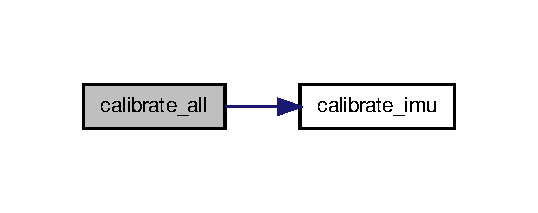
\includegraphics[width=258pt]{calibration_8h_a043045246cf217758281222214c4addc_cgraph}
\end{center}
\end{figure}


\hypertarget{calibration_8h_aecfc81d152db2843b5d1517729804d63}{\index{calibration.\-h@{calibration.\-h}!calibrate\-\_\-imu@{calibrate\-\_\-imu}}
\index{calibrate\-\_\-imu@{calibrate\-\_\-imu}!calibration.h@{calibration.\-h}}
\subsubsection[{calibrate\-\_\-imu}]{\setlength{\rightskip}{0pt plus 5cm}void calibrate\-\_\-imu (
\begin{DoxyParamCaption}
\item[{{\bf I\-M\-U\-\_\-\-D\-A\-T\-A\-\_\-\-S\-T\-R\-U\-C\-T} $\ast$}]{imu\-\_\-data}
\end{DoxyParamCaption}
)}}\label{calibration_8h_aecfc81d152db2843b5d1517729804d63}


Definition at line 14 of file calibration.\-c.



References I\-M\-U\-\_\-\-D\-A\-T\-A\-\_\-\-S\-T\-R\-U\-C\-T\-::acc, I\-M\-U\-\_\-\-D\-A\-T\-A\-\_\-\-S\-T\-R\-U\-C\-T\-::calibrated\-::acc, A\-C\-C\-\_\-\-B\-I\-A\-S\-\_\-\-X, A\-C\-C\-\_\-\-B\-I\-A\-S\-\_\-\-Y, A\-C\-C\-\_\-\-B\-I\-A\-S\-\_\-\-Z, A\-C\-C\-\_\-\-F\-S\-\_\-\-X, A\-C\-C\-\_\-\-F\-S\-\_\-\-Y, A\-C\-C\-\_\-\-F\-S\-\_\-\-Z, I\-M\-U\-\_\-\-D\-A\-T\-A\-\_\-\-S\-T\-R\-U\-C\-T\-::calib, I\-M\-U\-\_\-\-D\-A\-T\-A\-\_\-\-S\-T\-R\-U\-C\-T\-::calib\-\_\-temp, I\-M\-U\-\_\-\-D\-A\-T\-A\-\_\-\-S\-T\-R\-U\-C\-T\-::gyr, I\-M\-U\-\_\-\-D\-A\-T\-A\-\_\-\-S\-T\-R\-U\-C\-T\-::calibrated\-::gyr, G\-Y\-R\-\_\-\-B\-I\-A\-S\-\_\-\-X, G\-Y\-R\-\_\-\-B\-I\-A\-S\-\_\-\-Y, G\-Y\-R\-\_\-\-B\-I\-A\-S\-\_\-\-Z, G\-Y\-R\-\_\-\-F\-S\-\_\-\-X, G\-Y\-R\-\_\-\-F\-S\-\_\-\-Y, G\-Y\-R\-\_\-\-F\-S\-\_\-\-Z, I\-M\-U\-\_\-\-D\-A\-T\-A\-\_\-\-S\-T\-R\-U\-C\-T\-::mag, I\-M\-U\-\_\-\-D\-A\-T\-A\-\_\-\-S\-T\-R\-U\-C\-T\-::calibrated\-::mag, M\-A\-G\-\_\-\-B\-I\-A\-S\-\_\-\-X, M\-A\-G\-\_\-\-B\-I\-A\-S\-\_\-\-Y, M\-A\-G\-\_\-\-B\-I\-A\-S\-\_\-\-Z, M\-A\-G\-\_\-\-F\-S\-\_\-\-X, M\-A\-G\-\_\-\-F\-S\-\_\-\-Y, M\-A\-G\-\_\-\-F\-S\-\_\-\-Z, I\-M\-U\-\_\-\-D\-A\-T\-A\-\_\-\-S\-T\-R\-U\-C\-T\-::temp, D\-A\-T\-A\-\_\-\-X\-Y\-Z\-::x, D\-A\-T\-A\-\_\-\-X\-Y\-Z\-\_\-\-D\-O\-U\-B\-L\-E\-::x, D\-A\-T\-A\-\_\-\-X\-Y\-Z\-::y, D\-A\-T\-A\-\_\-\-X\-Y\-Z\-\_\-\-D\-O\-U\-B\-L\-E\-::y, D\-A\-T\-A\-\_\-\-X\-Y\-Z\-::z, and D\-A\-T\-A\-\_\-\-X\-Y\-Z\-\_\-\-D\-O\-U\-B\-L\-E\-::z.



Referenced by calibrate\-\_\-all().


\begin{DoxyCode}
\{
  \textcolor{comment}{// With this parameters, the vectors of acceleration and magnetic field will
       have norm = 1 theorically (i.e. in g or G)}
  imu\_data->\hyperlink{structIMU__DATA__STRUCT_aeffe3c3c5a7191a5cef16e7aab6c3795}{calib}.\hyperlink{structIMU__DATA__STRUCT_1_1calibrated_a281a7fdb40a05ed97388f18b9bb90c81}{acc}.\hyperlink{structDATA__XYZ__DOUBLE_a22868cc99a423900e7b82d015a5eb91f}{x} = ((double)imu\_data->\hyperlink{structIMU__DATA__STRUCT_a448f284bf44eb503affda586ad5fa9d2}{acc}.\hyperlink{structDATA__XYZ_a54c1596e9f9969fd9c21e8458024ecfb}{x}-\hyperlink{calibration_2calibration_8h_a355ea8f6ceed1e1d419a3ea2271bfca3}{ACC\_BIAS\_X}
      )/\hyperlink{calibration_2calibration_8h_a76e6967cb5a86ec34986b4583ac09831}{ACC\_FS\_X};
  imu\_data->\hyperlink{structIMU__DATA__STRUCT_aeffe3c3c5a7191a5cef16e7aab6c3795}{calib}.\hyperlink{structIMU__DATA__STRUCT_1_1calibrated_a281a7fdb40a05ed97388f18b9bb90c81}{acc}.\hyperlink{structDATA__XYZ__DOUBLE_a198a27b5df3b5b0bf461b0e481e22a82}{y} = ((double)imu\_data->\hyperlink{structIMU__DATA__STRUCT_a448f284bf44eb503affda586ad5fa9d2}{acc}.\hyperlink{structDATA__XYZ_a94bbb1c889bf53eb6a5fffa2b39322cf}{y}-\hyperlink{calibration_2calibration_8h_a34180f1c97e84a814ef181f62bf4b68f}{ACC\_BIAS\_Y}
      )/\hyperlink{calibration_2calibration_8h_a13d3aaab3b5800b11351cbd1246c8918}{ACC\_FS\_Y};
  imu\_data->\hyperlink{structIMU__DATA__STRUCT_aeffe3c3c5a7191a5cef16e7aab6c3795}{calib}.\hyperlink{structIMU__DATA__STRUCT_1_1calibrated_a281a7fdb40a05ed97388f18b9bb90c81}{acc}.\hyperlink{structDATA__XYZ__DOUBLE_a9556e8868c223ff3e28756ea18a284c0}{z} = ((double)imu\_data->\hyperlink{structIMU__DATA__STRUCT_a448f284bf44eb503affda586ad5fa9d2}{acc}.\hyperlink{structDATA__XYZ_a69e89ab0ec6e5d72fc5d54f62cc07fb5}{z}-\hyperlink{calibration_2calibration_8h_a794f762650b6f228ffb8d50d1323dbea}{ACC\_BIAS\_Z}
      )/\hyperlink{calibration_2calibration_8h_af1d3370cc0958289199c8c13470602d4}{ACC\_FS\_Z};
  
  imu\_data->\hyperlink{structIMU__DATA__STRUCT_aeffe3c3c5a7191a5cef16e7aab6c3795}{calib}.\hyperlink{structIMU__DATA__STRUCT_1_1calibrated_a2fde6c6759e0fda17e272c32096cb9ec}{mag}.\hyperlink{structDATA__XYZ__DOUBLE_a22868cc99a423900e7b82d015a5eb91f}{x} = ((double)imu\_data->\hyperlink{structIMU__DATA__STRUCT_a40c7df8b6d49297aa52873cfd9b60daa}{mag}.\hyperlink{structDATA__XYZ_a54c1596e9f9969fd9c21e8458024ecfb}{x}-\hyperlink{calibration_2calibration_8h_a355ea8f6ceed1e1d419a3ea2271bfca3}{ACC\_BIAS\_X}
      )/\hyperlink{calibration_2calibration_8h_a76e6967cb5a86ec34986b4583ac09831}{ACC\_FS\_X};
  imu\_data->\hyperlink{structIMU__DATA__STRUCT_aeffe3c3c5a7191a5cef16e7aab6c3795}{calib}.\hyperlink{structIMU__DATA__STRUCT_1_1calibrated_a2fde6c6759e0fda17e272c32096cb9ec}{mag}.\hyperlink{structDATA__XYZ__DOUBLE_a198a27b5df3b5b0bf461b0e481e22a82}{y} = ((double)imu\_data->\hyperlink{structIMU__DATA__STRUCT_a40c7df8b6d49297aa52873cfd9b60daa}{mag}.\hyperlink{structDATA__XYZ_a94bbb1c889bf53eb6a5fffa2b39322cf}{y}-\hyperlink{calibration_2calibration_8h_a34180f1c97e84a814ef181f62bf4b68f}{ACC\_BIAS\_Y}
      )/\hyperlink{calibration_2calibration_8h_a13d3aaab3b5800b11351cbd1246c8918}{ACC\_FS\_Y};
  imu\_data->\hyperlink{structIMU__DATA__STRUCT_aeffe3c3c5a7191a5cef16e7aab6c3795}{calib}.\hyperlink{structIMU__DATA__STRUCT_1_1calibrated_a2fde6c6759e0fda17e272c32096cb9ec}{mag}.\hyperlink{structDATA__XYZ__DOUBLE_a9556e8868c223ff3e28756ea18a284c0}{z} = ((double)imu\_data->\hyperlink{structIMU__DATA__STRUCT_a40c7df8b6d49297aa52873cfd9b60daa}{mag}.\hyperlink{structDATA__XYZ_a69e89ab0ec6e5d72fc5d54f62cc07fb5}{z}-\hyperlink{calibration_2calibration_8h_a794f762650b6f228ffb8d50d1323dbea}{ACC\_BIAS\_Z}
      )/\hyperlink{calibration_2calibration_8h_af1d3370cc0958289199c8c13470602d4}{ACC\_FS\_Z};
  
  \textcolor{comment}{// With this parameters, we consider right datasheet scale and we get in
       rad/s}
  imu\_data->\hyperlink{structIMU__DATA__STRUCT_aeffe3c3c5a7191a5cef16e7aab6c3795}{calib}.\hyperlink{structIMU__DATA__STRUCT_1_1calibrated_a8a54aded6ce608f1b7d2b4a0c52c248b}{gyr}.\hyperlink{structDATA__XYZ__DOUBLE_a22868cc99a423900e7b82d015a5eb91f}{x} = ((double)imu\_data->\hyperlink{structIMU__DATA__STRUCT_a0c1ac26626e4434a2ee124a1928a23a1}{gyr}.\hyperlink{structDATA__XYZ_a54c1596e9f9969fd9c21e8458024ecfb}{x}-\hyperlink{calibration_2calibration_8h_a69780ffe3a15aad4121fed56d5e47377}{GYR\_BIAS\_X}
      )/\hyperlink{calibration_2calibration_8h_a8fe84f8c6d39f41d8622fd0cbce3a522}{GYR\_FS\_X};
  imu\_data->\hyperlink{structIMU__DATA__STRUCT_aeffe3c3c5a7191a5cef16e7aab6c3795}{calib}.\hyperlink{structIMU__DATA__STRUCT_1_1calibrated_a8a54aded6ce608f1b7d2b4a0c52c248b}{gyr}.\hyperlink{structDATA__XYZ__DOUBLE_a198a27b5df3b5b0bf461b0e481e22a82}{y} = ((double)imu\_data->\hyperlink{structIMU__DATA__STRUCT_a0c1ac26626e4434a2ee124a1928a23a1}{gyr}.\hyperlink{structDATA__XYZ_a94bbb1c889bf53eb6a5fffa2b39322cf}{y}-\hyperlink{calibration_2calibration_8h_a69780ffe3a15aad4121fed56d5e47377}{GYR\_BIAS\_X}
      )/\hyperlink{calibration_2calibration_8h_a4be2e0fa7596546bb4699862d0fe4183}{GYR\_FS\_Y};
  imu\_data->\hyperlink{structIMU__DATA__STRUCT_aeffe3c3c5a7191a5cef16e7aab6c3795}{calib}.\hyperlink{structIMU__DATA__STRUCT_1_1calibrated_a8a54aded6ce608f1b7d2b4a0c52c248b}{gyr}.\hyperlink{structDATA__XYZ__DOUBLE_a9556e8868c223ff3e28756ea18a284c0}{z} = ((double)imu\_data->\hyperlink{structIMU__DATA__STRUCT_a0c1ac26626e4434a2ee124a1928a23a1}{gyr}.\hyperlink{structDATA__XYZ_a69e89ab0ec6e5d72fc5d54f62cc07fb5}{z}-\hyperlink{calibration_2calibration_8h_a69780ffe3a15aad4121fed56d5e47377}{GYR\_BIAS\_X}
      )/\hyperlink{calibration_2calibration_8h_aaee2ece0c43cc20d7c531ab79dcd06c8}{GYR\_FS\_Z};
  
  \textcolor{keywordflow}{return};
\}
\end{DoxyCode}


Here is the caller graph for this function\-:\nopagebreak
\begin{figure}[H]
\begin{center}
\leavevmode
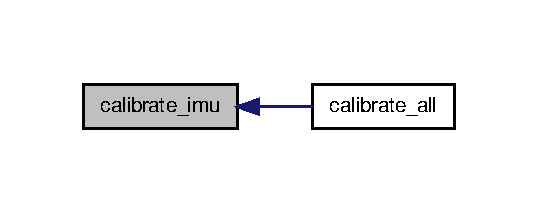
\includegraphics[width=258pt]{calibration_8h_aecfc81d152db2843b5d1517729804d63_icgraph}
\end{center}
\end{figure}



\include{acc__functions_8c}
\include{communication_8c}
\include{communication_8h}
\hypertarget{encoder__functions_8c}{\section{communication/encoder\-\_\-functions.c File Reference}
\label{encoder__functions_8c}\index{communication/encoder\-\_\-functions.\-c@{communication/encoder\-\_\-functions.\-c}}
}


Rev 0 -\/ 19/06/2013 R\-L\-E\-G project -\/ 2013.  


{\ttfamily \#include \char`\"{}encoder\-\_\-functions.\-h\char`\"{}}\\*
{\ttfamily \#include \char`\"{}spi\-\_\-functions.\-h\char`\"{}}\\*
Include dependency graph for encoder\-\_\-functions.\-c\-:\nopagebreak
\begin{figure}[H]
\begin{center}
\leavevmode
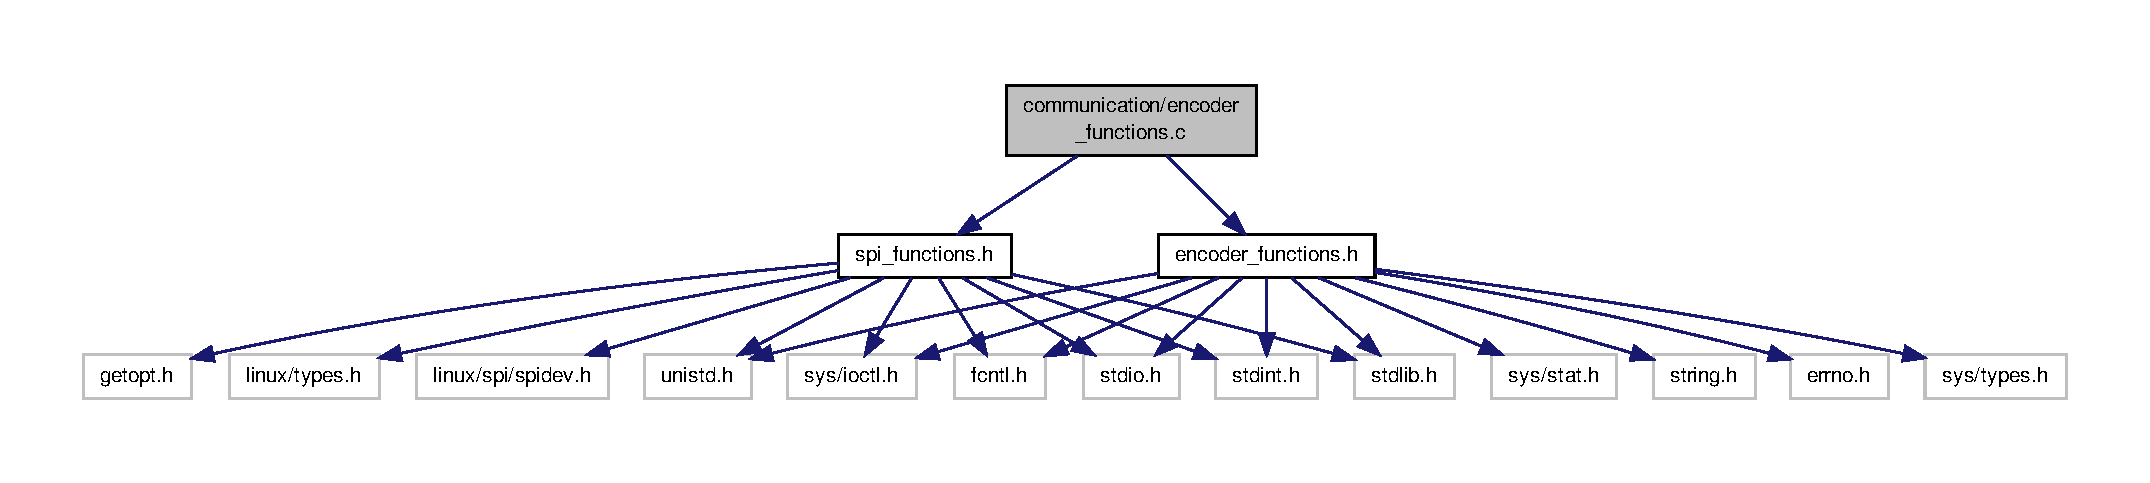
\includegraphics[width=350pt]{encoder__functions_8c__incl}
\end{center}
\end{figure}
\subsection*{Functions}
\begin{DoxyCompactItemize}
\item 
int \hyperlink{group__enc_gaebbe7b9d3c2571f7481cefacbe36c498}{enc\-\_\-zero\-\_\-set} (int \hyperlink{CommunicationV0_2communication_8c_a4788f0a5355494bc6c13690e28f43783}{spi\-\_\-dev})
\begin{DoxyCompactList}\small\item\em S\-E\-T Z\-E\-R\-O P\-O\-I\-N\-T. \end{DoxyCompactList}\item 
int \hyperlink{group__enc_ga813c09cc4d9af8b357fe440a9438e685}{enc\-\_\-read\-\_\-pos} (int \hyperlink{CommunicationV0_2communication_8c_a4788f0a5355494bc6c13690e28f43783}{spi\-\_\-dev}, unsigned short int $\ast$data)
\begin{DoxyCompactList}\small\item\em R\-E\-A\-D P\-O\-S\-I\-T\-I\-O\-N. \end{DoxyCompactList}\item 
int \hyperlink{group__enc_gad82fb44f2e735628ec95e003e4a1f93c}{enc\-\_\-wait\-\_\-for\-\_\-ack} (int \hyperlink{CommunicationV0_2communication_8c_a4788f0a5355494bc6c13690e28f43783}{spi\-\_\-dev}, uint8\-\_\-t ack, int max\-\_\-errors)
\begin{DoxyCompactList}\small\item\em send command and delay between reads \end{DoxyCompactList}\end{DoxyCompactItemize}


\subsection{Detailed Description}
Rev 0 -\/ 19/06/2013 R\-L\-E\-G project -\/ 2013. S\-P\-I communication between Gumstix Overo Fire and the A\-M\-T 203 encoder \begin{DoxyAuthor}{Author}
Claudia Ochoa 
\end{DoxyAuthor}
\begin{DoxyDate}{Date}
2012-\/2013 
\end{DoxyDate}


Definition in file \hyperlink{encoder__functions_8c_source}{encoder\-\_\-functions.\-c}.


\hypertarget{encoder__functions_8h}{
\section{communication/encoder\_\-functions.h File Reference}
\label{encoder__functions_8h}\index{communication/encoder\_\-functions.h@{communication/encoder\_\-functions.h}}
}


Rev 0 -\/ 18/06/2013 RLEG project -\/ 2013.  


{\ttfamily \#include $<$stdio.h$>$}\par
{\ttfamily \#include $<$stdint.h$>$}\par
{\ttfamily \#include $<$stdlib.h$>$}\par
{\ttfamily \#include $<$string.h$>$}\par
{\ttfamily \#include $<$errno.h$>$}\par
{\ttfamily \#include $<$unistd.h$>$}\par
{\ttfamily \#include $<$sys/types.h$>$}\par
{\ttfamily \#include $<$sys/stat.h$>$}\par
{\ttfamily \#include $<$sys/ioctl.h$>$}\par
{\ttfamily \#include $<$fcntl.h$>$}\par
Include dependency graph for encoder\_\-functions.h:This graph shows which files directly or indirectly include this file:\subsection*{Data Structures}
\begin{DoxyCompactItemize}
\item 
struct \hyperlink{structENC__DATA__STRUCT}{ENC\_\-DATA\_\-STRUCT}
\item 
struct \hyperlink{structENC__DATA__STRUCT_1_1calibrate}{ENC\_\-DATA\_\-STRUCT::calibrate}
\end{DoxyCompactItemize}
\subsection*{Defines}
\begin{DoxyCompactItemize}
\item 
\#define \hyperlink{encoder__functions_8h_aa90cac659d18e8ef6294c7ae337f6b58}{SUCCESS}~1
\item 
\#define \hyperlink{encoder__functions_8h_a6d58f9ac447476b4e084d7ca383f5183}{FAILURE}~-\/1
\item 
\#define \hyperlink{encoder__functions_8h_ac10b0f18ed2164776ad6843aa7908592}{ENCODER\_\-NO\_\-OP}~0x00
\item 
\#define \hyperlink{encoder__functions_8h_a24e6c0e05e904b10f56ae184da9e2aca}{ENCODER\_\-RD\_\-POS}~0x10
\item 
\#define \hyperlink{encoder__functions_8h_aa2fec4e0eb5a7b3668158a57952b9dbe}{ENCODER\_\-SET\_\-ZERO\_\-PT}~0x70
\item 
\#define \hyperlink{encoder__functions_8h_ab815abd4b9b825c60dbb04aad0d0e846}{ENCODER\_\-EEPROM\_\-WR}~0x80
\item 
\#define \hyperlink{encoder__functions_8h_aa3f0b6d222591f8f7332f74106eaa0ca}{ENCODER\_\-EEPROM\_\-RD}~0x90
\item 
\#define \hyperlink{encoder__functions_8h_a77c3a97f7312d858d04ec3b4e1fb2176}{ENCODER\_\-WAIT\_\-RESP}~0xA5
\item 
\#define \hyperlink{encoder__functions_8h_a9ec306f36d50c7375e74f0d1c55a3a67}{INT\_\-MAX}~5
\end{DoxyCompactItemize}
\subsection*{Functions}
\begin{DoxyCompactItemize}
\item 
int \hyperlink{group__enc_ga813c09cc4d9af8b357fe440a9438e685}{enc\_\-read\_\-pos} (int spi\_\-dev, unsigned short int $\ast$data)
\begin{DoxyCompactList}\small\item\em READ POSITION. \item\end{DoxyCompactList}\item 
int \hyperlink{group__enc_gaebbe7b9d3c2571f7481cefacbe36c498}{enc\_\-zero\_\-set} (int spi\_\-dev)
\begin{DoxyCompactList}\small\item\em SET ZERO POINT. \item\end{DoxyCompactList}\item 
int \hyperlink{group__enc_gad82fb44f2e735628ec95e003e4a1f93c}{enc\_\-wait\_\-for\_\-ack} (int spi\_\-dev, uint8\_\-t ack, int max\_\-errors)
\begin{DoxyCompactList}\small\item\em send command and delay between reads \item\end{DoxyCompactList}\end{DoxyCompactItemize}


\subsection{Detailed Description}
Rev 0 -\/ 18/06/2013 RLEG project -\/ 2013. main commmands of the AMT 203 encoder \begin{DoxyAuthor}{Author}
Claudia Ochoa 
\end{DoxyAuthor}
\begin{DoxyDate}{Date}
2012-\/2013 
\end{DoxyDate}


Definition in file \hyperlink{encoder__functions_8h_source}{encoder\_\-functions.h}.



\subsection{Define Documentation}
\hypertarget{encoder__functions_8h_aa3f0b6d222591f8f7332f74106eaa0ca}{
\index{encoder\_\-functions.h@{encoder\_\-functions.h}!ENCODER\_\-EEPROM\_\-RD@{ENCODER\_\-EEPROM\_\-RD}}
\index{ENCODER\_\-EEPROM\_\-RD@{ENCODER\_\-EEPROM\_\-RD}!encoder_functions.h@{encoder\_\-functions.h}}
\subsubsection[{ENCODER\_\-EEPROM\_\-RD}]{\setlength{\rightskip}{0pt plus 5cm}\#define ENCODER\_\-EEPROM\_\-RD~0x90}}
\label{encoder__functions_8h_aa3f0b6d222591f8f7332f74106eaa0ca}


Definition at line 34 of file encoder\_\-functions.h.

\hypertarget{encoder__functions_8h_ab815abd4b9b825c60dbb04aad0d0e846}{
\index{encoder\_\-functions.h@{encoder\_\-functions.h}!ENCODER\_\-EEPROM\_\-WR@{ENCODER\_\-EEPROM\_\-WR}}
\index{ENCODER\_\-EEPROM\_\-WR@{ENCODER\_\-EEPROM\_\-WR}!encoder_functions.h@{encoder\_\-functions.h}}
\subsubsection[{ENCODER\_\-EEPROM\_\-WR}]{\setlength{\rightskip}{0pt plus 5cm}\#define ENCODER\_\-EEPROM\_\-WR~0x80}}
\label{encoder__functions_8h_ab815abd4b9b825c60dbb04aad0d0e846}


Definition at line 33 of file encoder\_\-functions.h.



Referenced by enc\_\-zero\_\-set().

\hypertarget{encoder__functions_8h_ac10b0f18ed2164776ad6843aa7908592}{
\index{encoder\_\-functions.h@{encoder\_\-functions.h}!ENCODER\_\-NO\_\-OP@{ENCODER\_\-NO\_\-OP}}
\index{ENCODER\_\-NO\_\-OP@{ENCODER\_\-NO\_\-OP}!encoder_functions.h@{encoder\_\-functions.h}}
\subsubsection[{ENCODER\_\-NO\_\-OP}]{\setlength{\rightskip}{0pt plus 5cm}\#define ENCODER\_\-NO\_\-OP~0x00}}
\label{encoder__functions_8h_ac10b0f18ed2164776ad6843aa7908592}


Definition at line 30 of file encoder\_\-functions.h.



Referenced by enc\_\-read\_\-pos(), and enc\_\-wait\_\-for\_\-ack().

\hypertarget{encoder__functions_8h_a24e6c0e05e904b10f56ae184da9e2aca}{
\index{encoder\_\-functions.h@{encoder\_\-functions.h}!ENCODER\_\-RD\_\-POS@{ENCODER\_\-RD\_\-POS}}
\index{ENCODER\_\-RD\_\-POS@{ENCODER\_\-RD\_\-POS}!encoder_functions.h@{encoder\_\-functions.h}}
\subsubsection[{ENCODER\_\-RD\_\-POS}]{\setlength{\rightskip}{0pt plus 5cm}\#define ENCODER\_\-RD\_\-POS~0x10}}
\label{encoder__functions_8h_a24e6c0e05e904b10f56ae184da9e2aca}


Definition at line 31 of file encoder\_\-functions.h.



Referenced by enc\_\-read\_\-pos().

\hypertarget{encoder__functions_8h_aa2fec4e0eb5a7b3668158a57952b9dbe}{
\index{encoder\_\-functions.h@{encoder\_\-functions.h}!ENCODER\_\-SET\_\-ZERO\_\-PT@{ENCODER\_\-SET\_\-ZERO\_\-PT}}
\index{ENCODER\_\-SET\_\-ZERO\_\-PT@{ENCODER\_\-SET\_\-ZERO\_\-PT}!encoder_functions.h@{encoder\_\-functions.h}}
\subsubsection[{ENCODER\_\-SET\_\-ZERO\_\-PT}]{\setlength{\rightskip}{0pt plus 5cm}\#define ENCODER\_\-SET\_\-ZERO\_\-PT~0x70}}
\label{encoder__functions_8h_aa2fec4e0eb5a7b3668158a57952b9dbe}


Definition at line 32 of file encoder\_\-functions.h.



Referenced by enc\_\-zero\_\-set().

\hypertarget{encoder__functions_8h_a77c3a97f7312d858d04ec3b4e1fb2176}{
\index{encoder\_\-functions.h@{encoder\_\-functions.h}!ENCODER\_\-WAIT\_\-RESP@{ENCODER\_\-WAIT\_\-RESP}}
\index{ENCODER\_\-WAIT\_\-RESP@{ENCODER\_\-WAIT\_\-RESP}!encoder_functions.h@{encoder\_\-functions.h}}
\subsubsection[{ENCODER\_\-WAIT\_\-RESP}]{\setlength{\rightskip}{0pt plus 5cm}\#define ENCODER\_\-WAIT\_\-RESP~0xA5}}
\label{encoder__functions_8h_a77c3a97f7312d858d04ec3b4e1fb2176}


Definition at line 37 of file encoder\_\-functions.h.



Referenced by enc\_\-wait\_\-for\_\-ack().

\hypertarget{encoder__functions_8h_a6d58f9ac447476b4e084d7ca383f5183}{
\index{encoder\_\-functions.h@{encoder\_\-functions.h}!FAILURE@{FAILURE}}
\index{FAILURE@{FAILURE}!encoder_functions.h@{encoder\_\-functions.h}}
\subsubsection[{FAILURE}]{\setlength{\rightskip}{0pt plus 5cm}\#define FAILURE~-\/1}}
\label{encoder__functions_8h_a6d58f9ac447476b4e084d7ca383f5183}


Definition at line 27 of file encoder\_\-functions.h.

\hypertarget{encoder__functions_8h_a9ec306f36d50c7375e74f0d1c55a3a67}{
\index{encoder\_\-functions.h@{encoder\_\-functions.h}!INT\_\-MAX@{INT\_\-MAX}}
\index{INT\_\-MAX@{INT\_\-MAX}!encoder_functions.h@{encoder\_\-functions.h}}
\subsubsection[{INT\_\-MAX}]{\setlength{\rightskip}{0pt plus 5cm}\#define INT\_\-MAX~5}}
\label{encoder__functions_8h_a9ec306f36d50c7375e74f0d1c55a3a67}


Definition at line 39 of file encoder\_\-functions.h.



Referenced by enc\_\-read\_\-pos(), and enc\_\-zero\_\-set().

\hypertarget{encoder__functions_8h_aa90cac659d18e8ef6294c7ae337f6b58}{
\index{encoder\_\-functions.h@{encoder\_\-functions.h}!SUCCESS@{SUCCESS}}
\index{SUCCESS@{SUCCESS}!encoder_functions.h@{encoder\_\-functions.h}}
\subsubsection[{SUCCESS}]{\setlength{\rightskip}{0pt plus 5cm}\#define SUCCESS~1}}
\label{encoder__functions_8h_aa90cac659d18e8ef6294c7ae337f6b58}


Definition at line 26 of file encoder\_\-functions.h.


\include{gpio__functions_8c}
\include{gpio__functions_8h}
\include{gyr__functions_8c}
\include{imu__functions_8h}
\include{imu__regs_8h}
\include{mag__functions_8c}
\include{spi__functions_8c}
\include{spi__functions_8h}
\hypertarget{control_8c}{
\section{control/control.c File Reference}
\label{control_8c}\index{control/control.c@{control/control.c}}
}
\subsection*{Functions}
\begin{DoxyCompactItemize}
\item 
void \hyperlink{control_8c_affcc9c00d6ed4b976ae2d0e53b60f51f}{control\_\-main} (\hyperlink{threads__linux_8c_a2a2a647912528f7aa86812528dbfe02f}{t\_\-task\_\-1\_\-global},\&\hyperlink{threads__linux_8c_a3cfea12cbe9ca7f1681c950e4cd68606}{imu\_\-data},\&\hyperlink{main2_8c_a5650ece8c3a277c7f158d75ae65265fa}{eff\_\-data},\&\hyperlink{main2_8c_abc42e18d2909e9bc119316283f4ed9db}{mra\_\-data})
\begin{DoxyCompactList}\small\item\em Function: control\_\-main Summary: Calculate the control signal. \item\end{DoxyCompactList}\end{DoxyCompactItemize}


\subsection{Function Documentation}
\hypertarget{control_8c_affcc9c00d6ed4b976ae2d0e53b60f51f}{
\index{control.c@{control.c}!control\_\-main@{control\_\-main}}
\index{control\_\-main@{control\_\-main}!control.c@{control.c}}
\subsubsection[{control\_\-main}]{\setlength{\rightskip}{0pt plus 5cm}void control\_\-main ({\bf t\_\-task\_\-1\_\-global}, \/  \& {\em imu\_\-data}, \/  \& {\em eff\_\-data}, \/  \& {\em mra\_\-data})}}
\label{control_8c_affcc9c00d6ed4b976ae2d0e53b60f51f}


Function: control\_\-main Summary: Calculate the control signal. 


\begin{DoxyParams}{Parameters}
\item[{\em t\_\-task\_\-1\_\-global}]containing the ... \item[{\em imu\_\-data}]containing data from accelerometer, gyrometer and magnetometer \item[{\em eff\_\-data}]containing data from load cell \item[{\em mra\_\-data}]struct containing the control signal\end{DoxyParams}
\begin{DoxyReturn}{Returns}
nothing 
\end{DoxyReturn}


Definition at line 11 of file control.c.



References IMU\_\-DATA\_\-STRUCT::acc, imu\_\-data, mra\_\-data, MRA\_\-DATA\_\-STRUCT::v\_\-ctl, DATA\_\-XYZ::x, and DATA\_\-XYZ::z.




\begin{DoxyCode}
11                                                                     {
12 int t_gait = 0;
13 int gait_cycle = 2000000;//Gait cycle takes 2 seconds
14 int heelstrike_threshold = 3;
15 
16         //In case of heel strike the gait cycle starts
17         //Heel strike detection: module of acceleration vector (which has compone
      nts in x and z axis) higher than threshold.
18         if ((((imu_data->acc.x)^2 + (imu_data->acc.z)^2)^0.5) > heelstrike_thresh
      old){
19           t_gait = 0;
20         //Between 10% and 60% of the gait cycle, actuation voltage is 0V
21         } else if (t_gait>(0.1*gait_cycle) && t_gait<=(0.6*gait_cycle)){
22           //control voltage 0V
23           mra_data.v_ctl=0;
24         //More than 60% of the gait cycle, set actuation voltage to 4V.
25         } else if (t_gait>(0.6*gait_cycle) && t_gait<(0.8*gait_cycle)){
26           mra_data.v_ctl=4000;
27         }
28 
29 }
\end{DoxyCode}



\include{control_8h}
\hypertarget{datalogger_8c}{\section{datalogger.\-c File Reference}
\label{datalogger_8c}\index{datalogger.\-c@{datalogger.\-c}}
}
{\ttfamily \#include $<$stdlib.\-h$>$}\\*
{\ttfamily \#include $<$stdio.\-h$>$}\\*
{\ttfamily \#include $<$string.\-h$>$}\\*
{\ttfamily \#include $<$pthread.\-h$>$}\\*
{\ttfamily \#include \char`\"{}gdatalogger/gqueue.\-h\char`\"{}}\\*
{\ttfamily \#include \char`\"{}gdatalogger/gmatlabdatafile.\-h\char`\"{}}\\*
{\ttfamily \#include \char`\"{}gdatalogger/gdatalogger.\-h\char`\"{}}\\*
{\ttfamily \#include \char`\"{}communication/communication.\-h\char`\"{}}\\*
{\ttfamily \#include \char`\"{}datalogger.\-h\char`\"{}}\\*
Include dependency graph for datalogger.\-c\-:\nopagebreak
\begin{figure}[H]
\begin{center}
\leavevmode
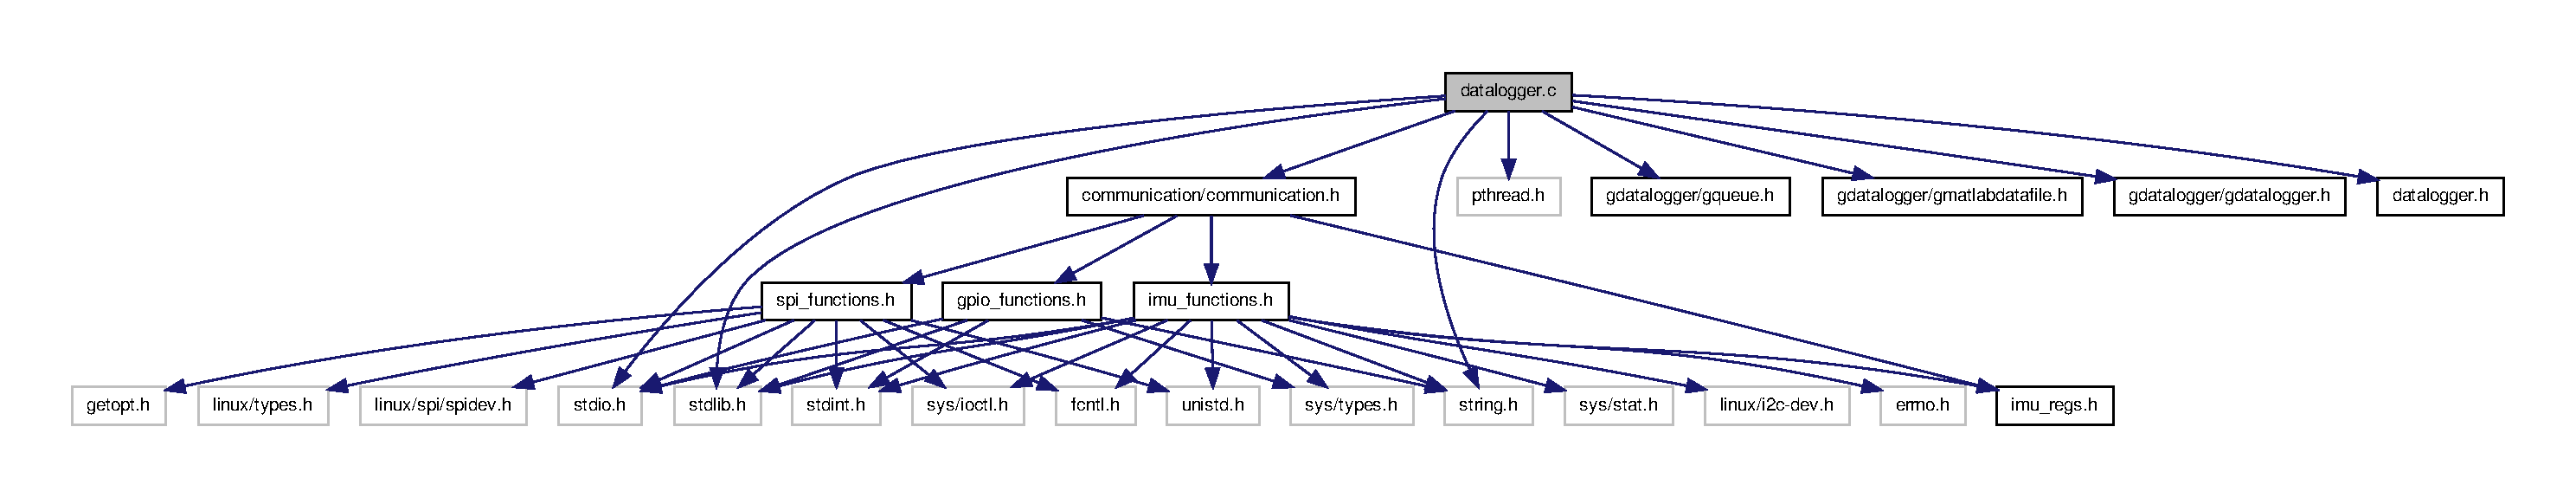
\includegraphics[width=350pt]{datalogger_8c__incl}
\end{center}
\end{figure}
\subsection*{Functions}
\begin{DoxyCompactItemize}
\item 
int \hyperlink{datalogger_8c_a54b06d9395b2e370a5a72beb7f9524b2}{datalogger\-\_\-lock\-\_\-mutex} (void)
\item 
int \hyperlink{datalogger_8c_a85453211c0c809083c36cc56b275aeeb}{datalogger\-\_\-unlock\-\_\-mutex} (void)
\item 
int \hyperlink{datalogger_8c_a1977ef253746fd8c008a3641d9822551}{datalogger\-\_\-init} (void)
\item 
int \hyperlink{datalogger_8c_ad22dbe9e235e7ae5737a23796d13ffbd}{datalogger\-\_\-close} (void)
\item 
int \hyperlink{datalogger_8c_a2aedecfce53e1935a41615ceaf378013}{datalogger\-\_\-write\-\_\-file} (void)
\item 
int \hyperlink{datalogger_8c_a25bb814a0877f419ae09b08cd7e91ee9}{datalogger\-\_\-update\-\_\-\-I\-P\-C} (void)
\item 
int \hyperlink{datalogger_8c_ad89a56e2f057ace8c28d78eb67703e7d}{datalogger\-\_\-update} (double t\-\_\-s, double t\-\_\-control\-\_\-exec\-\_\-s, double t\-\_\-ui\-\_\-exec\-\_\-s, double t0\-\_\-s, \hyperlink{structIMU__DATA__STRUCT}{I\-M\-U\-\_\-\-D\-A\-T\-A\-\_\-\-S\-T\-R\-U\-C\-T} $\ast$pimu\-\_\-data, \hyperlink{structEFF__DATA__STRUCT}{E\-F\-F\-\_\-\-D\-A\-T\-A\-\_\-\-S\-T\-R\-U\-C\-T} $\ast$peff\-\_\-data, \hyperlink{structMRA__DATA__STRUCT}{M\-R\-A\-\_\-\-D\-A\-T\-A\-\_\-\-S\-T\-R\-U\-C\-T} $\ast$pmra\-\_\-data)
\item 
int \hyperlink{datalogger_8c_afb69d166f8d53042825174cee225ea49}{datalogger\-\_\-set\-\_\-\-Ts} (double Ts)
\item 
int \hyperlink{datalogger_8c_a46fd1290d9ee97d5fc7171e1e0dcb0aa}{datalogger\-\_\-status} (void)
\item 
int \hyperlink{datalogger_8c_a1f254ef380d595d6605c10811fd0dee6}{datalogger\-\_\-start} (void)
\item 
int \hyperlink{datalogger_8c_aae2ffbc6cbf8f1cfecceb42c5139530a}{datalogger\-\_\-stop} (void)
\item 
int \hyperlink{datalogger_8c_a29bc3190cba1f225ad3b2eed899a6762}{datalogger\-\_\-file\-\_\-exists} (const char $\ast$filename)
\end{DoxyCompactItemize}
\subsection*{Variables}
\begin{DoxyCompactItemize}
\item 
\hyperlink{structGDATALOGGER}{G\-D\-A\-T\-A\-L\-O\-G\-G\-E\-R} \hyperlink{datalogger_8c_abe3b9c2c4e21e79c7b046b5986d13acc}{g\-Data\-Logger}
\item 
unsigned int \hyperlink{datalogger_8c_a35e8fbe04b90452afdc3c1be16ff6187}{datalogger\-\_\-initialized} = \hyperlink{datalogger_8h_a4602a65fdfa920dfe832cfa50b7ee4c8}{D\-A\-T\-A\-L\-O\-G\-G\-E\-R\-\_\-\-N\-O\-T\-\_\-\-I\-N\-I\-T\-I\-A\-L\-I\-Z\-E\-D}
\item 
unsigned int \hyperlink{datalogger_8c_a185c3ede96449d14f330fe5ac664e799}{datalogger\-\_\-running} = \hyperlink{datalogger_8h_a1a224da36800f52f56f30619849f7f5d}{D\-A\-T\-A\-L\-O\-G\-G\-E\-R\-\_\-\-N\-O\-T\-\_\-\-R\-U\-N\-N\-I\-N\-G}
\item 
pthread\-\_\-mutex\-\_\-t \hyperlink{datalogger_8c_a824d6f7fd1d3898ba0b1100ba37875c6}{datalogger\-\_\-mutex} = P\-T\-H\-R\-E\-A\-D\-\_\-\-M\-U\-T\-E\-X\-\_\-\-I\-N\-I\-T\-I\-A\-L\-I\-Z\-E\-R
\end{DoxyCompactItemize}


\subsection{Function Documentation}
\hypertarget{datalogger_8c_ad22dbe9e235e7ae5737a23796d13ffbd}{\index{datalogger.\-c@{datalogger.\-c}!datalogger\-\_\-close@{datalogger\-\_\-close}}
\index{datalogger\-\_\-close@{datalogger\-\_\-close}!datalogger.c@{datalogger.\-c}}
\subsubsection[{datalogger\-\_\-close}]{\setlength{\rightskip}{0pt plus 5cm}int datalogger\-\_\-close (
\begin{DoxyParamCaption}
\item[{void}]{}
\end{DoxyParamCaption}
)}}\label{datalogger_8c_ad22dbe9e235e7ae5737a23796d13ffbd}


Definition at line 215 of file datalogger.\-c.



References D\-A\-T\-A\-L\-O\-G\-G\-E\-R\-\_\-\-E\-R\-R\-O\-R\-\_\-\-N\-O\-T\-\_\-\-I\-N\-I\-T\-I\-A\-L\-I\-Z\-E\-D, D\-A\-T\-A\-L\-O\-G\-G\-E\-R\-\_\-\-I\-N\-I\-T\-I\-A\-L\-I\-Z\-E\-D, datalogger\-\_\-initialized, datalogger\-\_\-lock\-\_\-mutex(), datalogger\-\_\-mutex, D\-A\-T\-A\-L\-O\-G\-G\-E\-R\-\_\-\-N\-O\-T\-\_\-\-I\-N\-I\-T\-I\-A\-L\-I\-Z\-E\-D, D\-A\-T\-A\-L\-O\-G\-G\-E\-R\-\_\-\-S\-U\-C\-C\-E\-S\-S, datalogger\-\_\-unlock\-\_\-mutex(), g\-Data\-Logger\-\_\-\-Close(), and g\-Data\-Logger\-\_\-\-Matfile\-Update().



Referenced by main(), and threads\-\_\-linux\-\_\-init().


\begin{DoxyCode}
\{
\textcolor{preprocessor}{    #if DATALOGGER\_MODULE\_ENABLED}
\textcolor{preprocessor}{}        \hyperlink{datalogger_8c_a54b06d9395b2e370a5a72beb7f9524b2}{datalogger\_lock\_mutex}();
        \textcolor{keywordflow}{if}(\hyperlink{datalogger_8c_a35e8fbe04b90452afdc3c1be16ff6187}{datalogger\_initialized} != 
      \hyperlink{datalogger_8h_a684c343d340004b77ca2b782934c96ca}{DATALOGGER\_INITIALIZED})
    \{
            \hyperlink{datalogger_8c_a85453211c0c809083c36cc56b275aeeb}{datalogger\_unlock\_mutex}();
        \textcolor{keywordflow}{return} \hyperlink{datalogger_8h_a60df7fe0e61b757ad6a9db106b0eb43e}{DATALOGGER\_ERROR\_NOT\_INITIALIZED}
      ;
    \}

    \hyperlink{gdatalogger_8c_a05dc8ce832b941280d7de26057992640}{gDataLogger\_MatfileUpdate}(&\hyperlink{datalogger_8c_abe3b9c2c4e21e79c7b046b5986d13acc}{gDataLogger})
      ; \textcolor{comment}{// Update data}
    \hyperlink{gdatalogger_8c_a0ac95f84c6ee484c4ad0351530f1c468}{gDataLogger\_Close}(&\hyperlink{datalogger_8c_abe3b9c2c4e21e79c7b046b5986d13acc}{gDataLogger}); \textcolor{comment}{// Close
       datalogger}

    \hyperlink{datalogger_8c_a35e8fbe04b90452afdc3c1be16ff6187}{datalogger\_initialized} = \hyperlink{datalogger_8h_a4602a65fdfa920dfe832cfa50b7ee4c8}{DATALOGGER\_NOT\_INITIALIZED}
      ;
    \hyperlink{datalogger_8c_a85453211c0c809083c36cc56b275aeeb}{datalogger\_unlock\_mutex}();

\textcolor{preprocessor}{        #if ANU\_COMPILE\_FOR\_XENOMAI}
\textcolor{preprocessor}{}    rt\_mutex\_delete(&\hyperlink{datalogger_8c_a824d6f7fd1d3898ba0b1100ba37875c6}{datalogger\_mutex});
\textcolor{preprocessor}{        #endif  //ANU\_COMPILE\_FOR\_XENOMAI}
\textcolor{preprocessor}{}
\textcolor{preprocessor}{    #endif //DATALOGGER\_MODULE\_ENABLED}
\textcolor{preprocessor}{}
    \textcolor{keywordflow}{return} \hyperlink{datalogger_8h_abddebaf71d26d40183fccbb1a766b983}{DATALOGGER\_SUCCESS};
\}
\end{DoxyCode}


Here is the call graph for this function\-:\nopagebreak
\begin{figure}[H]
\begin{center}
\leavevmode
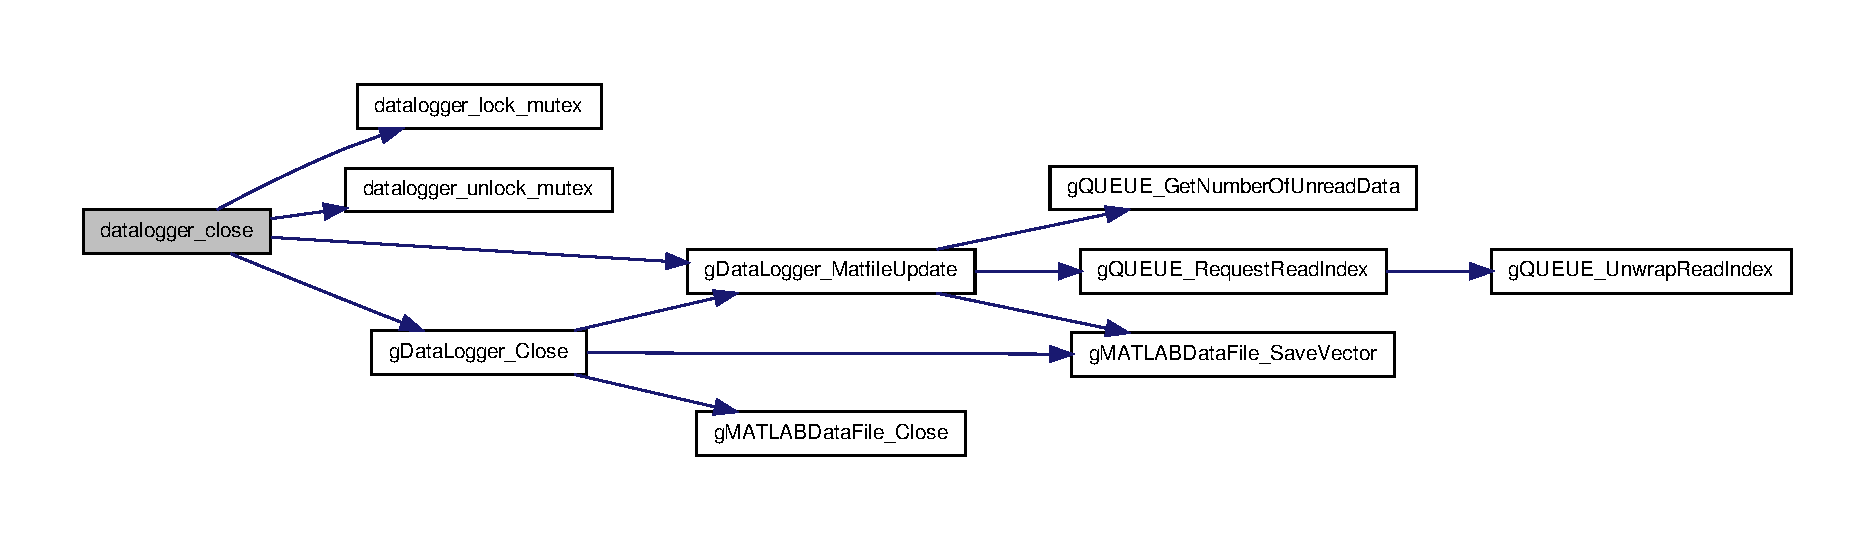
\includegraphics[width=350pt]{datalogger_8c_ad22dbe9e235e7ae5737a23796d13ffbd_cgraph}
\end{center}
\end{figure}




Here is the caller graph for this function\-:\nopagebreak
\begin{figure}[H]
\begin{center}
\leavevmode
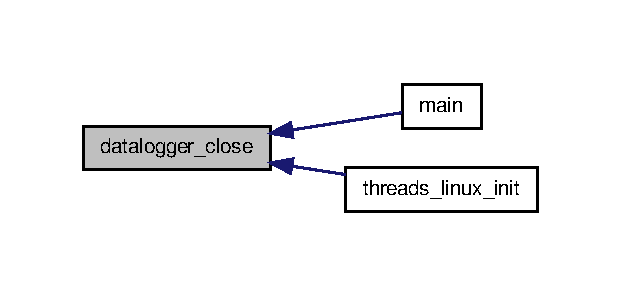
\includegraphics[width=298pt]{datalogger_8c_ad22dbe9e235e7ae5737a23796d13ffbd_icgraph}
\end{center}
\end{figure}


\hypertarget{datalogger_8c_a29bc3190cba1f225ad3b2eed899a6762}{\index{datalogger.\-c@{datalogger.\-c}!datalogger\-\_\-file\-\_\-exists@{datalogger\-\_\-file\-\_\-exists}}
\index{datalogger\-\_\-file\-\_\-exists@{datalogger\-\_\-file\-\_\-exists}!datalogger.c@{datalogger.\-c}}
\subsubsection[{datalogger\-\_\-file\-\_\-exists}]{\setlength{\rightskip}{0pt plus 5cm}int datalogger\-\_\-file\-\_\-exists (
\begin{DoxyParamCaption}
\item[{const char $\ast$}]{filename}
\end{DoxyParamCaption}
)}}\label{datalogger_8c_a29bc3190cba1f225ad3b2eed899a6762}


Definition at line 618 of file datalogger.\-c.



References D\-A\-T\-A\-L\-O\-G\-G\-E\-R\-\_\-\-F\-A\-I\-L\-U\-R\-E, and D\-A\-T\-A\-L\-O\-G\-G\-E\-R\-\_\-\-S\-U\-C\-C\-E\-S\-S.



Referenced by datalogger\-\_\-init().


\begin{DoxyCode}
\{
    FILE *file;
    \textcolor{keywordflow}{if}((file = fopen(filename, \textcolor{stringliteral}{"r"})))
    \{
        fclose(file);
        \textcolor{keywordflow}{return} \hyperlink{datalogger_8h_abddebaf71d26d40183fccbb1a766b983}{DATALOGGER\_SUCCESS};
    \}
    \textcolor{keywordflow}{return} \hyperlink{datalogger_8h_ac52138ca42979f6e1f1d589020ff9f83}{DATALOGGER\_FAILURE};
\}
\end{DoxyCode}


Here is the caller graph for this function\-:\nopagebreak
\begin{figure}[H]
\begin{center}
\leavevmode
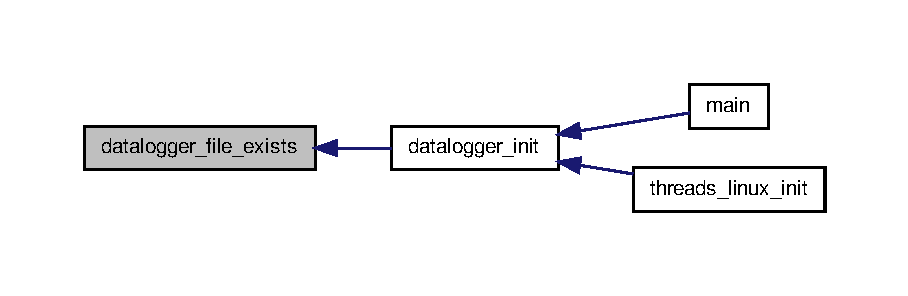
\includegraphics[width=350pt]{datalogger_8c_a29bc3190cba1f225ad3b2eed899a6762_icgraph}
\end{center}
\end{figure}


\hypertarget{datalogger_8c_a1977ef253746fd8c008a3641d9822551}{\index{datalogger.\-c@{datalogger.\-c}!datalogger\-\_\-init@{datalogger\-\_\-init}}
\index{datalogger\-\_\-init@{datalogger\-\_\-init}!datalogger.c@{datalogger.\-c}}
\subsubsection[{datalogger\-\_\-init}]{\setlength{\rightskip}{0pt plus 5cm}int datalogger\-\_\-init (
\begin{DoxyParamCaption}
\item[{void}]{}
\end{DoxyParamCaption}
)}}\label{datalogger_8c_a1977ef253746fd8c008a3641d9822551}


Definition at line 41 of file datalogger.\-c.



References D\-A\-T\-A\-L\-O\-G\-G\-E\-R\-\_\-\-F\-A\-I\-L\-U\-R\-E, datalogger\-\_\-file\-\_\-exists(), D\-A\-T\-A\-L\-O\-G\-G\-E\-R\-\_\-\-F\-I\-L\-E\-\_\-\-N\-A\-M\-E, D\-A\-T\-A\-L\-O\-G\-G\-E\-R\-\_\-\-F\-O\-L\-D\-E\-R, D\-A\-T\-A\-L\-O\-G\-G\-E\-R\-\_\-\-I\-N\-I\-T\-I\-A\-L\-I\-Z\-E\-D, datalogger\-\_\-initialized, datalogger\-\_\-lock\-\_\-mutex(), D\-A\-T\-A\-L\-O\-G\-G\-E\-R\-\_\-\-L\-O\-G\-\_\-\-C\-A\-L\-I\-B\-R\-A\-T\-E\-D\-\_\-\-I\-M\-U, D\-A\-T\-A\-L\-O\-G\-G\-E\-R\-\_\-\-L\-O\-G\-\_\-\-E\-F\-F\-O\-R\-T\-S, D\-A\-T\-A\-L\-O\-G\-G\-E\-R\-\_\-\-L\-O\-G\-\_\-\-E\-X\-E\-C\-T\-I\-M\-E\-S, D\-A\-T\-A\-L\-O\-G\-G\-E\-R\-\_\-\-L\-O\-G\-\_\-\-M\-R\-A, D\-A\-T\-A\-L\-O\-G\-G\-E\-R\-\_\-\-L\-O\-G\-\_\-\-R\-A\-W\-\_\-\-I\-M\-U, D\-A\-T\-A\-L\-O\-G\-G\-E\-R\-\_\-\-L\-O\-G\-\_\-\-T\-I\-M\-E, datalogger\-\_\-mutex, D\-A\-T\-A\-L\-O\-G\-G\-E\-R\-\_\-\-N\-O\-T\-\_\-\-R\-U\-N\-N\-I\-N\-G, datalogger\-\_\-running, D\-A\-T\-A\-L\-O\-G\-G\-E\-R\-\_\-\-S\-T\-A\-N\-D\-A\-R\-D\-\_\-\-Q\-U\-E\-U\-E\-\_\-\-S\-I\-Z\-E, D\-A\-T\-A\-L\-O\-G\-G\-E\-R\-\_\-\-S\-U\-C\-C\-E\-S\-S, datalogger\-\_\-unlock\-\_\-mutex(), g\-Data\-Logger\-\_\-\-Declare\-Variable(), g\-Data\-Logger\-\_\-\-Init(), and g\-Data\-Logger\-\_\-\-Insert\-Variable().



Referenced by main(), and threads\-\_\-linux\-\_\-init().


\begin{DoxyCode}
\{
\textcolor{preprocessor}{    #if DATALOGGER\_MODULE\_ENABLED}
\textcolor{preprocessor}{}    \textcolor{keywordtype}{double} enabled\_variables[16][1];
    \textcolor{keywordtype}{char} datalogger\_filename[256];
\textcolor{preprocessor}{        #if ANU\_COMPILE\_FOR\_XENOMAI}
\textcolor{preprocessor}{}    rt\_mutex\_create(&\hyperlink{datalogger_8c_a824d6f7fd1d3898ba0b1100ba37875c6}{datalogger\_mutex},\textcolor{stringliteral}{"Data Logger Mutex"});
\textcolor{preprocessor}{        #endif}
\textcolor{preprocessor}{}    \hyperlink{datalogger_8c_a54b06d9395b2e370a5a72beb7f9524b2}{datalogger\_lock\_mutex}();

    \textcolor{keywordflow}{if}(\hyperlink{datalogger_8c_a35e8fbe04b90452afdc3c1be16ff6187}{datalogger\_initialized} == \hyperlink{datalogger_8h_a684c343d340004b77ca2b782934c96ca}{DATALOGGER\_INITIALIZED}
      )
    \{
        \hyperlink{datalogger_8c_a85453211c0c809083c36cc56b275aeeb}{datalogger\_unlock\_mutex}();
        \textcolor{keywordflow}{return} \hyperlink{datalogger_8h_ac52138ca42979f6e1f1d589020ff9f83}{DATALOGGER\_FAILURE};
    \}

    \hyperlink{datalogger_8c_a185c3ede96449d14f330fe5ac664e799}{datalogger\_running} = \hyperlink{datalogger_8h_a1a224da36800f52f56f30619849f7f5d}{DATALOGGER\_NOT\_RUNNING}
      ;

        \textcolor{comment}{// Init datalogger}
    strcpy(datalogger\_filename, \hyperlink{datalogger_8h_a29791c024463d251eeab6973a0299e7b}{DATALOGGER\_FOLDER});
    strcat(datalogger\_filename, \textcolor{stringliteral}{"/"});
    strcat(datalogger\_filename, \hyperlink{datalogger_8h_a23bf1fb88a2adab92e7c477d927b241c}{DATALOGGER\_FILE\_NAME});
    strcat(datalogger\_filename, \textcolor{stringliteral}{".mat"});
\textcolor{preprocessor}{        #if DATALOGGER\_ENABLE\_NEW\_FILE\_ENNUMERATION}
\textcolor{preprocessor}{}    \textcolor{keywordtype}{char} datalogger\_tmp[256];
    \textcolor{keywordtype}{int} i = 0;
    \textcolor{keywordflow}{if}(\hyperlink{datalogger_8c_a29bc3190cba1f225ad3b2eed899a6762}{datalogger\_file\_exists}(datalogger\_filename) == 
      \hyperlink{datalogger_8h_abddebaf71d26d40183fccbb1a766b983}{DATALOGGER\_SUCCESS}) \textcolor{comment}{// File exists}
    \{
        strcpy(datalogger\_tmp, \hyperlink{datalogger_8h_a29791c024463d251eeab6973a0299e7b}{DATALOGGER\_FOLDER});
        strcat(datalogger\_tmp, \textcolor{stringliteral}{"/"});
        strcat(datalogger\_tmp, \hyperlink{datalogger_8h_a23bf1fb88a2adab92e7c477d927b241c}{DATALOGGER\_FILE\_NAME});
        strcat(datalogger\_tmp, \textcolor{stringliteral}{"\_%d.mat"});
        \textcolor{keywordflow}{do}
        \{
            sprintf(datalogger\_filename, datalogger\_tmp, ++i);
        \}
        \textcolor{keywordflow}{while}((\hyperlink{datalogger_8c_a29bc3190cba1f225ad3b2eed899a6762}{datalogger\_file\_exists}(datalogger\_filename
      ) == \hyperlink{datalogger_8h_abddebaf71d26d40183fccbb1a766b983}{DATALOGGER\_SUCCESS}) && (i<100));
        \textcolor{keywordflow}{if}(i == 100)
        \{
            \hyperlink{datalogger_8c_a85453211c0c809083c36cc56b275aeeb}{datalogger\_unlock\_mutex}();
            \textcolor{keywordflow}{return} \hyperlink{datalogger_8h_ac52138ca42979f6e1f1d589020ff9f83}{DATALOGGER\_FAILURE};
        \}
    \}
\textcolor{preprocessor}{        #endif //DATALOGGER\_ENABLE\_NEW\_FILE\_ENNUMERATION}
\textcolor{preprocessor}{}
    \textcolor{keywordflow}{if}(!\hyperlink{gdatalogger_8c_ab5eeb22d60836d57bae0dde821337045}{gDataLogger\_Init}(&\hyperlink{datalogger_8c_abe3b9c2c4e21e79c7b046b5986d13acc}{gDataLogger}, 
      datalogger\_filename, NULL))
    \{
        \hyperlink{datalogger_8c_a85453211c0c809083c36cc56b275aeeb}{datalogger\_unlock\_mutex}();
        \textcolor{keywordflow}{return} \hyperlink{datalogger_8h_ac52138ca42979f6e1f1d589020ff9f83}{DATALOGGER\_FAILURE};
    \}

        \textcolor{comment}{// Declare variables}
        \textcolor{comment}{// Arguments for gDataLogger\_DeclareVariable:}
        \textcolor{comment}{// datalogger pointer, variable name, units, number of rows, number of
       columns, queue size}

        \textcolor{comment}{// Variable that tells MATLAB which variables are enabled}
    enabled\_variables[0][0] = (double) \hyperlink{datalogger_8h_a9796dd7063d48a850456a4542c5a5fb5}{DATALOGGER\_LOG\_TIME};
    enabled\_variables[1][0] = (double) \hyperlink{datalogger_8h_ade62d89afc68e01d78fa75ae491a9980}{DATALOGGER\_LOG\_EXECTIMES}
      ;
    enabled\_variables[2][0] = (double) \hyperlink{datalogger_8h_a1c623aa143d8b2e0d507e23425a02275}{DATALOGGER\_LOG\_RAW\_IMU}
      ;
    enabled\_variables[3][0] = (double) \hyperlink{datalogger_8h_aa80b147e8c585f7f630658025c24cd8c}{DATALOGGER\_LOG\_CALIBRATED\_IMU}
      ;
    enabled\_variables[4][0] = (double) \hyperlink{datalogger_8h_a210c5f76b25cb165226a337189a9715f}{DATALOGGER\_LOG\_EFFORTS}
      ;
    enabled\_variables[5][0] = (double) \hyperlink{datalogger_8h_ab2e9ad670e20d71c67230b1f064a0dcb}{DATALOGGER\_LOG\_MRA};
    \textcolor{comment}{//enabled\_variables[12][0] = (double)
       DATALOGGER\_LOG\_LOCAL\_COORDINATE\_SYSTEM;}
    \textcolor{comment}{//enabled\_variables[13][0] = (double) DATALOGGER\_LOG\_LOCAL\_FIELDS;}
    \textcolor{comment}{//enabled\_variables[14][0] = (double) DATALOGGER\_LOG\_ESTIMATOR;}
    \textcolor{comment}{//enabled\_variables[15][0] = (double) DATALOGGER\_LOG\_CONTROLLERS;}

    \hyperlink{gdatalogger_8c_a3f8f2b3c3f5edc72c3a1887965a544c1}{gDataLogger\_DeclareVariable}(&\hyperlink{datalogger_8c_abe3b9c2c4e21e79c7b046b5986d13acc}{gDataLogger}
      , \textcolor{stringliteral}{"enabled\_vars"}, \textcolor{stringliteral}{""}, 6, 1, 1);
    \hyperlink{gdatalogger_8c_a32674e7c2afa8b78e99a0070cf4bcaf9}{gDataLogger\_InsertVariable}(&\hyperlink{datalogger_8c_abe3b9c2c4e21e79c7b046b5986d13acc}{gDataLogger}
      , \textcolor{stringliteral}{"enabled\_vars"}, &enabled\_variables[0][0]);

\textcolor{preprocessor}{        #if DATALOGGER\_LOG\_TIME}
\textcolor{preprocessor}{}        \hyperlink{gdatalogger_8c_a3f8f2b3c3f5edc72c3a1887965a544c1}{gDataLogger\_DeclareVariable}(&\hyperlink{datalogger_8c_abe3b9c2c4e21e79c7b046b5986d13acc}{gDataLogger}
      , \textcolor{stringliteral}{"t"}, \textcolor{stringliteral}{"s"}, 1, 1, \hyperlink{datalogger_8h_ac244ccff7e47d7f9e79c1b606664f4fa}{DATALOGGER\_STANDARD\_QUEUE\_SIZE});
    \hyperlink{gdatalogger_8c_a3f8f2b3c3f5edc72c3a1887965a544c1}{gDataLogger\_DeclareVariable}(&\hyperlink{datalogger_8c_abe3b9c2c4e21e79c7b046b5986d13acc}{gDataLogger}
      , \textcolor{stringliteral}{"Ts"}, \textcolor{stringliteral}{"s"}, 1, 1, 1);
\textcolor{preprocessor}{    #endif // DATALOGGER\_LOG\_TIME}
\textcolor{preprocessor}{}
\textcolor{preprocessor}{    #if DATALOGGER\_LOG\_EXECTIMES}
\textcolor{preprocessor}{}    \hyperlink{gdatalogger_8c_a3f8f2b3c3f5edc72c3a1887965a544c1}{gDataLogger\_DeclareVariable}(&\hyperlink{datalogger_8c_abe3b9c2c4e21e79c7b046b5986d13acc}{gDataLogger}
      , \textcolor{stringliteral}{"t\_control\_exec"}, \textcolor{stringliteral}{"s"}, 1, 1, \hyperlink{datalogger_8h_ac244ccff7e47d7f9e79c1b606664f4fa}{DATALOGGER\_STANDARD\_QUEUE\_SIZE}
      );
    \hyperlink{gdatalogger_8c_a3f8f2b3c3f5edc72c3a1887965a544c1}{gDataLogger\_DeclareVariable}(&\hyperlink{datalogger_8c_abe3b9c2c4e21e79c7b046b5986d13acc}{gDataLogger}
      , \textcolor{stringliteral}{"t\_ui\_exec"}, \textcolor{stringliteral}{"s"}, 1, 1, \hyperlink{datalogger_8h_ac244ccff7e47d7f9e79c1b606664f4fa}{DATALOGGER\_STANDARD\_QUEUE\_SIZE}
      );
\textcolor{preprocessor}{    #endif // DATALOGGER\_LOG\_EXECTIMES}
\textcolor{preprocessor}{}
\textcolor{preprocessor}{        #if DATALOGGER\_LOG\_RAW\_IMU}
\textcolor{preprocessor}{}        \hyperlink{gdatalogger_8c_a3f8f2b3c3f5edc72c3a1887965a544c1}{gDataLogger\_DeclareVariable}(&\hyperlink{datalogger_8c_abe3b9c2c4e21e79c7b046b5986d13acc}{gDataLogger}
      , \textcolor{stringliteral}{"imu\_accelerometer\_x\_raw"}, \textcolor{stringliteral}{"raw"}, 1, 1, \hyperlink{datalogger_8h_ac244ccff7e47d7f9e79c1b606664f4fa}{DATALOGGER\_STANDARD\_QUEUE\_SIZE}
      );
        \hyperlink{gdatalogger_8c_a3f8f2b3c3f5edc72c3a1887965a544c1}{gDataLogger\_DeclareVariable}(&\hyperlink{datalogger_8c_abe3b9c2c4e21e79c7b046b5986d13acc}{gDataLogger}
      , \textcolor{stringliteral}{"imu\_accelerometer\_y\_raw"}, \textcolor{stringliteral}{"raw"}, 1, 1, \hyperlink{datalogger_8h_ac244ccff7e47d7f9e79c1b606664f4fa}{DATALOGGER\_STANDARD\_QUEUE\_SIZE}
      );
        \hyperlink{gdatalogger_8c_a3f8f2b3c3f5edc72c3a1887965a544c1}{gDataLogger\_DeclareVariable}(&\hyperlink{datalogger_8c_abe3b9c2c4e21e79c7b046b5986d13acc}{gDataLogger}
      , \textcolor{stringliteral}{"imu\_accelerometer\_z\_raw"}, \textcolor{stringliteral}{"raw"}, 1, 1, \hyperlink{datalogger_8h_ac244ccff7e47d7f9e79c1b606664f4fa}{DATALOGGER\_STANDARD\_QUEUE\_SIZE}
      );
        \hyperlink{gdatalogger_8c_a3f8f2b3c3f5edc72c3a1887965a544c1}{gDataLogger\_DeclareVariable}(&\hyperlink{datalogger_8c_abe3b9c2c4e21e79c7b046b5986d13acc}{gDataLogger}
      , \textcolor{stringliteral}{"imu\_magnetometer\_x\_raw"}, \textcolor{stringliteral}{"raw"}, 1, 1, \hyperlink{datalogger_8h_ac244ccff7e47d7f9e79c1b606664f4fa}{DATALOGGER\_STANDARD\_QUEUE\_SIZE}
      );
        \hyperlink{gdatalogger_8c_a3f8f2b3c3f5edc72c3a1887965a544c1}{gDataLogger\_DeclareVariable}(&\hyperlink{datalogger_8c_abe3b9c2c4e21e79c7b046b5986d13acc}{gDataLogger}
      , \textcolor{stringliteral}{"imu\_magnetometer\_y\_raw"}, \textcolor{stringliteral}{"raw"}, 1, 1, \hyperlink{datalogger_8h_ac244ccff7e47d7f9e79c1b606664f4fa}{DATALOGGER\_STANDARD\_QUEUE\_SIZE}
      );
        \hyperlink{gdatalogger_8c_a3f8f2b3c3f5edc72c3a1887965a544c1}{gDataLogger\_DeclareVariable}(&\hyperlink{datalogger_8c_abe3b9c2c4e21e79c7b046b5986d13acc}{gDataLogger}
      , \textcolor{stringliteral}{"imu\_magnetometer\_z\_raw"}, \textcolor{stringliteral}{"raw"}, 1, 1, \hyperlink{datalogger_8h_ac244ccff7e47d7f9e79c1b606664f4fa}{DATALOGGER\_STANDARD\_QUEUE\_SIZE}
      );
        \hyperlink{gdatalogger_8c_a3f8f2b3c3f5edc72c3a1887965a544c1}{gDataLogger\_DeclareVariable}(&\hyperlink{datalogger_8c_abe3b9c2c4e21e79c7b046b5986d13acc}{gDataLogger}
      , \textcolor{stringliteral}{"imu\_gyrometer\_x\_raw"}, \textcolor{stringliteral}{"raw"}, 1, 1, \hyperlink{datalogger_8h_ac244ccff7e47d7f9e79c1b606664f4fa}{DATALOGGER\_STANDARD\_QUEUE\_SIZE}
      );
        \hyperlink{gdatalogger_8c_a3f8f2b3c3f5edc72c3a1887965a544c1}{gDataLogger\_DeclareVariable}(&\hyperlink{datalogger_8c_abe3b9c2c4e21e79c7b046b5986d13acc}{gDataLogger}
      , \textcolor{stringliteral}{"imu\_gyrometer\_y\_raw"}, \textcolor{stringliteral}{"raw"}, 1, 1, \hyperlink{datalogger_8h_ac244ccff7e47d7f9e79c1b606664f4fa}{DATALOGGER\_STANDARD\_QUEUE\_SIZE}
      );
        \hyperlink{gdatalogger_8c_a3f8f2b3c3f5edc72c3a1887965a544c1}{gDataLogger\_DeclareVariable}(&\hyperlink{datalogger_8c_abe3b9c2c4e21e79c7b046b5986d13acc}{gDataLogger}
      , \textcolor{stringliteral}{"imu\_gyrometer\_z\_raw"}, \textcolor{stringliteral}{"raw"}, 1, 1, \hyperlink{datalogger_8h_ac244ccff7e47d7f9e79c1b606664f4fa}{DATALOGGER\_STANDARD\_QUEUE\_SIZE}
      );
    \hyperlink{gdatalogger_8c_a3f8f2b3c3f5edc72c3a1887965a544c1}{gDataLogger\_DeclareVariable}(&\hyperlink{datalogger_8c_abe3b9c2c4e21e79c7b046b5986d13acc}{gDataLogger}
      , \textcolor{stringliteral}{"imu\_valid\_data"}, \textcolor{stringliteral}{""}, 1, 1, \hyperlink{datalogger_8h_ac244ccff7e47d7f9e79c1b606664f4fa}{DATALOGGER\_STANDARD\_QUEUE\_SIZE}
      );
\textcolor{preprocessor}{        #endif // DATALOGGER\_LOG\_IMU}
\textcolor{preprocessor}{}        
\textcolor{preprocessor}{    #if DATALOGGER\_LOG\_EFFORTS}
\textcolor{preprocessor}{}    \hyperlink{gdatalogger_8c_a3f8f2b3c3f5edc72c3a1887965a544c1}{gDataLogger\_DeclareVariable}(&\hyperlink{datalogger_8c_abe3b9c2c4e21e79c7b046b5986d13acc}{gDataLogger}
      , \textcolor{stringliteral}{"Vin0"}, \textcolor{stringliteral}{"mV"}, 1, 1, \hyperlink{datalogger_8h_ac244ccff7e47d7f9e79c1b606664f4fa}{DATALOGGER\_STANDARD\_QUEUE\_SIZE}
      );
    \hyperlink{gdatalogger_8c_a3f8f2b3c3f5edc72c3a1887965a544c1}{gDataLogger\_DeclareVariable}(&\hyperlink{datalogger_8c_abe3b9c2c4e21e79c7b046b5986d13acc}{gDataLogger}
      , \textcolor{stringliteral}{"Vin0\_valid\_data"}, \textcolor{stringliteral}{""}, 1, 1, \hyperlink{datalogger_8h_ac244ccff7e47d7f9e79c1b606664f4fa}{DATALOGGER\_STANDARD\_QUEUE\_SIZE}
      );
\textcolor{preprocessor}{    #endif}
\textcolor{preprocessor}{}    
\textcolor{preprocessor}{    #if DATALOGGER\_LOG\_MRA}
\textcolor{preprocessor}{}    \hyperlink{gdatalogger_8c_a3f8f2b3c3f5edc72c3a1887965a544c1}{gDataLogger\_DeclareVariable}(&\hyperlink{datalogger_8c_abe3b9c2c4e21e79c7b046b5986d13acc}{gDataLogger}
      , \textcolor{stringliteral}{"v\_ctl"}, \textcolor{stringliteral}{"mV"}, 1, 1, \hyperlink{datalogger_8h_ac244ccff7e47d7f9e79c1b606664f4fa}{DATALOGGER\_STANDARD\_QUEUE\_SIZE}
      );
    \hyperlink{gdatalogger_8c_a3f8f2b3c3f5edc72c3a1887965a544c1}{gDataLogger\_DeclareVariable}(&\hyperlink{datalogger_8c_abe3b9c2c4e21e79c7b046b5986d13acc}{gDataLogger}
      , \textcolor{stringliteral}{"v\_ctl\_read"}, \textcolor{stringliteral}{"mV"}, 1, 1, \hyperlink{datalogger_8h_ac244ccff7e47d7f9e79c1b606664f4fa}{DATALOGGER\_STANDARD\_QUEUE\_SIZE}
      );
\textcolor{preprocessor}{    #endif}
\textcolor{preprocessor}{}
\textcolor{preprocessor}{    #if DATALOGGER\_LOG\_CALIBRATED\_IMU}
\textcolor{preprocessor}{}    \hyperlink{gdatalogger_8c_a3f8f2b3c3f5edc72c3a1887965a544c1}{gDataLogger\_DeclareVariable}(&\hyperlink{datalogger_8c_abe3b9c2c4e21e79c7b046b5986d13acc}{gDataLogger}
      , \textcolor{stringliteral}{"imu\_accelerometer\_x\_g"}, \textcolor{stringliteral}{"g"}, 1, 1, \hyperlink{datalogger_8h_ac244ccff7e47d7f9e79c1b606664f4fa}{DATALOGGER\_STANDARD\_QUEUE\_SIZE}
      );
    \hyperlink{gdatalogger_8c_a3f8f2b3c3f5edc72c3a1887965a544c1}{gDataLogger\_DeclareVariable}(&\hyperlink{datalogger_8c_abe3b9c2c4e21e79c7b046b5986d13acc}{gDataLogger}
      , \textcolor{stringliteral}{"imu\_accelerometer\_y\_g"}, \textcolor{stringliteral}{"g"}, 1, 1, \hyperlink{datalogger_8h_ac244ccff7e47d7f9e79c1b606664f4fa}{DATALOGGER\_STANDARD\_QUEUE\_SIZE}
      );
    \hyperlink{gdatalogger_8c_a3f8f2b3c3f5edc72c3a1887965a544c1}{gDataLogger\_DeclareVariable}(&\hyperlink{datalogger_8c_abe3b9c2c4e21e79c7b046b5986d13acc}{gDataLogger}
      , \textcolor{stringliteral}{"imu\_accelerometer\_z\_g"}, \textcolor{stringliteral}{"g"}, 1, 1, \hyperlink{datalogger_8h_ac244ccff7e47d7f9e79c1b606664f4fa}{DATALOGGER\_STANDARD\_QUEUE\_SIZE}
      );
    \hyperlink{gdatalogger_8c_a3f8f2b3c3f5edc72c3a1887965a544c1}{gDataLogger\_DeclareVariable}(&\hyperlink{datalogger_8c_abe3b9c2c4e21e79c7b046b5986d13acc}{gDataLogger}
      , \textcolor{stringliteral}{"imu\_magnetometer\_x\_B"}, \textcolor{stringliteral}{"B"}, 1, 1, \hyperlink{datalogger_8h_ac244ccff7e47d7f9e79c1b606664f4fa}{DATALOGGER\_STANDARD\_QUEUE\_SIZE}
      );
    \hyperlink{gdatalogger_8c_a3f8f2b3c3f5edc72c3a1887965a544c1}{gDataLogger\_DeclareVariable}(&\hyperlink{datalogger_8c_abe3b9c2c4e21e79c7b046b5986d13acc}{gDataLogger}
      , \textcolor{stringliteral}{"imu\_magnetometer\_y\_B"}, \textcolor{stringliteral}{"B"}, 1, 1, \hyperlink{datalogger_8h_ac244ccff7e47d7f9e79c1b606664f4fa}{DATALOGGER\_STANDARD\_QUEUE\_SIZE}
      );
    \hyperlink{gdatalogger_8c_a3f8f2b3c3f5edc72c3a1887965a544c1}{gDataLogger\_DeclareVariable}(&\hyperlink{datalogger_8c_abe3b9c2c4e21e79c7b046b5986d13acc}{gDataLogger}
      , \textcolor{stringliteral}{"imu\_magnetometer\_z\_B"}, \textcolor{stringliteral}{"B"}, 1, 1, \hyperlink{datalogger_8h_ac244ccff7e47d7f9e79c1b606664f4fa}{DATALOGGER\_STANDARD\_QUEUE\_SIZE}
      );
    \hyperlink{gdatalogger_8c_a3f8f2b3c3f5edc72c3a1887965a544c1}{gDataLogger\_DeclareVariable}(&\hyperlink{datalogger_8c_abe3b9c2c4e21e79c7b046b5986d13acc}{gDataLogger}
      , \textcolor{stringliteral}{"imu\_gyrometer\_x\_rads"}, \textcolor{stringliteral}{"rads"}, 1, 1, \hyperlink{datalogger_8h_ac244ccff7e47d7f9e79c1b606664f4fa}{DATALOGGER\_STANDARD\_QUEUE\_SIZE}
      );
    \hyperlink{gdatalogger_8c_a3f8f2b3c3f5edc72c3a1887965a544c1}{gDataLogger\_DeclareVariable}(&\hyperlink{datalogger_8c_abe3b9c2c4e21e79c7b046b5986d13acc}{gDataLogger}
      , \textcolor{stringliteral}{"imu\_gyrometer\_y\_rads"}, \textcolor{stringliteral}{"rads"}, 1, 1, \hyperlink{datalogger_8h_ac244ccff7e47d7f9e79c1b606664f4fa}{DATALOGGER\_STANDARD\_QUEUE\_SIZE}
      );
    \hyperlink{gdatalogger_8c_a3f8f2b3c3f5edc72c3a1887965a544c1}{gDataLogger\_DeclareVariable}(&\hyperlink{datalogger_8c_abe3b9c2c4e21e79c7b046b5986d13acc}{gDataLogger}
      , \textcolor{stringliteral}{"imu\_gyrometer\_z\_rads"}, \textcolor{stringliteral}{"rads"}, 1, 1, \hyperlink{datalogger_8h_ac244ccff7e47d7f9e79c1b606664f4fa}{DATALOGGER\_STANDARD\_QUEUE\_SIZE}
      );
    \hyperlink{gdatalogger_8c_a3f8f2b3c3f5edc72c3a1887965a544c1}{gDataLogger\_DeclareVariable}(&\hyperlink{datalogger_8c_abe3b9c2c4e21e79c7b046b5986d13acc}{gDataLogger}
      , \textcolor{stringliteral}{"imu\_calibrated\_valid\_data"}, \textcolor{stringliteral}{""}, 1, 1, \hyperlink{datalogger_8h_ac244ccff7e47d7f9e79c1b606664f4fa}{DATALOGGER\_STANDARD\_QUEUE\_SIZE}
      );
    \textcolor{comment}{//gDataLogger\_DeclareVariable(&gDataLogger,
       "imu\_calibrated\_valid\_accelerometer\_data", "", 1, 1, DATALOGGER\_STANDARD\_QUEUE\_SIZE);}
    \textcolor{comment}{//gDataLogger\_DeclareVariable(&gDataLogger,
       "imu\_calibrated\_valid\_gyrometer\_data", "", 1, 1, DATALOGGER\_STANDARD\_QUEUE\_SIZE);}
    \textcolor{comment}{//gDataLogger\_DeclareVariable(&gDataLogger,
       "imu\_calibrated\_valid\_magnetometer\_data", "", 1, 1, DATALOGGER\_STANDARD\_QUEUE\_SIZE);}
\textcolor{preprocessor}{    #endif // DATALOGGER\_LOG\_CALIBRATED\_IMU}
\textcolor{preprocessor}{}

\textcolor{comment}{/*}
\textcolor{comment}{    #if DATALOGGER\_LOG\_LOCAL\_COORDINATE\_SYSTEM}
\textcolor{comment}{    gDataLogger\_DeclareVariable(&gDataLogger, "initial\_altitude", "m", 1, 1,
       1);}
\textcolor{comment}{    gDataLogger\_DeclareVariable(&gDataLogger, "initial\_latitude", "radians", 1,
       1, 1);}
\textcolor{comment}{    gDataLogger\_DeclareVariable(&gDataLogger, "initial\_longitude", "radians",
       1, 1, 1);}
\textcolor{comment}{    gDataLogger\_DeclareVariable(&gDataLogger, "initial\_ecef\_x", "m", 1, 1, 1);}
\textcolor{comment}{    gDataLogger\_DeclareVariable(&gDataLogger, "initial\_ecef\_y", "m", 1, 1, 1);}
\textcolor{comment}{    gDataLogger\_DeclareVariable(&gDataLogger, "initial\_ecef\_z", "m", 1, 1, 1);}
\textcolor{comment}{    gDataLogger\_DeclareVariable(&gDataLogger, "rotation\_matrix", "matrix", 3,
       3, 1);}
\textcolor{comment}{    #endif // DATALOGGER\_LOG\_LOCAL\_COORDINATE\_SYSTEM}
\textcolor{comment}{}
\textcolor{comment}{    #if DATALOGGER\_LOG\_LOCAL\_FIELDS}
\textcolor{comment}{    gDataLogger\_DeclareVariable(&gDataLogger, "local\_magnetic", "field", 3, 1,
       1);}
\textcolor{comment}{    gDataLogger\_DeclareVariable(&gDataLogger, "local\_gravity", "field", 3, 1,
       1);}
\textcolor{comment}{    gDataLogger\_DeclareVariable(&gDataLogger, "magnetic\_magnitude", "uT", 1, 1,
       1);}
\textcolor{comment}{    gDataLogger\_DeclareVariable(&gDataLogger, "gravity\_magnitude", "ms2", 1, 1,
       1);}
\textcolor{comment}{    #endif // DATALOGGER\_LOG\_LOCAL\_FIELDS}
\textcolor{comment}{}
\textcolor{comment}{    #if DATALOGGER\_LOG\_ESTIMATOR}
\textcolor{comment}{    gDataLogger\_DeclareVariable(&gDataLogger, "estimated\_roll\_angle\_radians",
       "radians", 1, 1, DATALOGGER\_STANDARD\_QUEUE\_SIZE);}
\textcolor{comment}{    gDataLogger\_DeclareVariable(&gDataLogger, "estimated\_pitch\_angle\_radians",
       "radians", 1, 1, DATALOGGER\_STANDARD\_QUEUE\_SIZE);}
\textcolor{comment}{    gDataLogger\_DeclareVariable(&gDataLogger, "estimated\_yaw\_angle\_radians",
       "radians", 1, 1, DATALOGGER\_STANDARD\_QUEUE\_SIZE);}
\textcolor{comment}{    gDataLogger\_DeclareVariable(&gDataLogger, "estimated\_q0", "quaternion", 1,
       1, DATALOGGER\_STANDARD\_QUEUE\_SIZE);}
\textcolor{comment}{    gDataLogger\_DeclareVariable(&gDataLogger, "estimated\_q1", "quaternion", 1,
       1, DATALOGGER\_STANDARD\_QUEUE\_SIZE);}
\textcolor{comment}{    gDataLogger\_DeclareVariable(&gDataLogger, "estimated\_q2", "quaternion", 1,
       1, DATALOGGER\_STANDARD\_QUEUE\_SIZE);}
\textcolor{comment}{    gDataLogger\_DeclareVariable(&gDataLogger, "estimated\_q3", "quaternion", 1,
       1, DATALOGGER\_STANDARD\_QUEUE\_SIZE);}
\textcolor{comment}{    gDataLogger\_DeclareVariable(&gDataLogger, "estimated\_x\_position\_meters",
       "meters", 1, 1, DATALOGGER\_STANDARD\_QUEUE\_SIZE);}
\textcolor{comment}{    gDataLogger\_DeclareVariable(&gDataLogger, "estimated\_y\_position\_meters",
       "meters", 1, 1, DATALOGGER\_STANDARD\_QUEUE\_SIZE);}
\textcolor{comment}{    gDataLogger\_DeclareVariable(&gDataLogger, "estimated\_z\_position\_meters",
       "meters", 1, 1, DATALOGGER\_STANDARD\_QUEUE\_SIZE);}
\textcolor{comment}{    gDataLogger\_DeclareVariable(&gDataLogger,
       "estimated\_x\_velocity\_meters\_second", "meters", 1, 1, DATALOGGER\_STANDARD\_QUEUE\_SIZE);}
\textcolor{comment}{    gDataLogger\_DeclareVariable(&gDataLogger,
       "estimated\_y\_velocity\_meters\_second", "meters", 1, 1, DATALOGGER\_STANDARD\_QUEUE\_SIZE);}
\textcolor{comment}{    gDataLogger\_DeclareVariable(&gDataLogger,
       "estimated\_z\_velocity\_meters\_second", "meters", 1, 1, DATALOGGER\_STANDARD\_QUEUE\_SIZE);}
\textcolor{comment}{    #endif // DATALOGGER\_LOG\_ESTIMATOR}
\textcolor{comment}{}
\textcolor{comment}{    #if DATALOGGER\_LOG\_CONTROLLERS}
\textcolor{comment}{    gDataLogger\_DeclareVariable(&gDataLogger,
       "control\_roll\_angle\_trim\_radians", "radians", 1, 1, DATALOGGER\_STANDARD\_QUEUE\_SIZE);}
\textcolor{comment}{    gDataLogger\_DeclareVariable(&gDataLogger,
       "control\_pitch\_angle\_trim\_radians", "radians", 1, 1, DATALOGGER\_STANDARD\_QUEUE\_SIZE);}
\textcolor{comment}{    gDataLogger\_DeclareVariable(&gDataLogger, "control\_yaw\_angle\_trim\_radians",
       "radians", 1, 1, DATALOGGER\_STANDARD\_QUEUE\_SIZE);}
\textcolor{comment}{    gDataLogger\_DeclareVariable(&gDataLogger, "control\_left\_aileron\_trim",
       "us", 1, 1, DATALOGGER\_STANDARD\_QUEUE\_SIZE);}
\textcolor{comment}{    gDataLogger\_DeclareVariable(&gDataLogger, "control\_right\_aileron\_trim",
       "us", 1, 1, DATALOGGER\_STANDARD\_QUEUE\_SIZE);}
\textcolor{comment}{    gDataLogger\_DeclareVariable(&gDataLogger, "control\_elevator\_trim", "us", 1,
       1, DATALOGGER\_STANDARD\_QUEUE\_SIZE);}
\textcolor{comment}{    gDataLogger\_DeclareVariable(&gDataLogger, "control\_rudder\_trim", "us", 1,
       1, DATALOGGER\_STANDARD\_QUEUE\_SIZE);}
\textcolor{comment}{    gDataLogger\_DeclareVariable(&gDataLogger,
       "control\_roll\_angle\_reference\_radians", "radians", 1, 1, DATALOGGER\_STANDARD\_QUEUE\_SIZE);}
\textcolor{comment}{    gDataLogger\_DeclareVariable(&gDataLogger,
       "control\_pitch\_angle\_reference\_radians", "radians", 1, 1, DATALOGGER\_STANDARD\_QUEUE\_SIZE);}
\textcolor{comment}{    gDataLogger\_DeclareVariable(&gDataLogger,
       "control\_yaw\_angle\_reference\_radians", "radians", 1, 1, DATALOGGER\_STANDARD\_QUEUE\_SIZE);}
\textcolor{comment}{    #endif // DATALOGGER\_LOG\_CONTROLLERS}
\textcolor{comment}{*/}
    \hyperlink{datalogger_8c_a35e8fbe04b90452afdc3c1be16ff6187}{datalogger\_initialized} = \hyperlink{datalogger_8h_a684c343d340004b77ca2b782934c96ca}{DATALOGGER\_INITIALIZED}
      ;
    \hyperlink{datalogger_8c_a85453211c0c809083c36cc56b275aeeb}{datalogger\_unlock\_mutex}();
\textcolor{preprocessor}{    #endif //DATALOGGER\_MODULE\_ENABLED}
\textcolor{preprocessor}{}
    \textcolor{keywordflow}{return} \hyperlink{datalogger_8h_abddebaf71d26d40183fccbb1a766b983}{DATALOGGER\_SUCCESS};
\}
\end{DoxyCode}


Here is the call graph for this function\-:\nopagebreak
\begin{figure}[H]
\begin{center}
\leavevmode
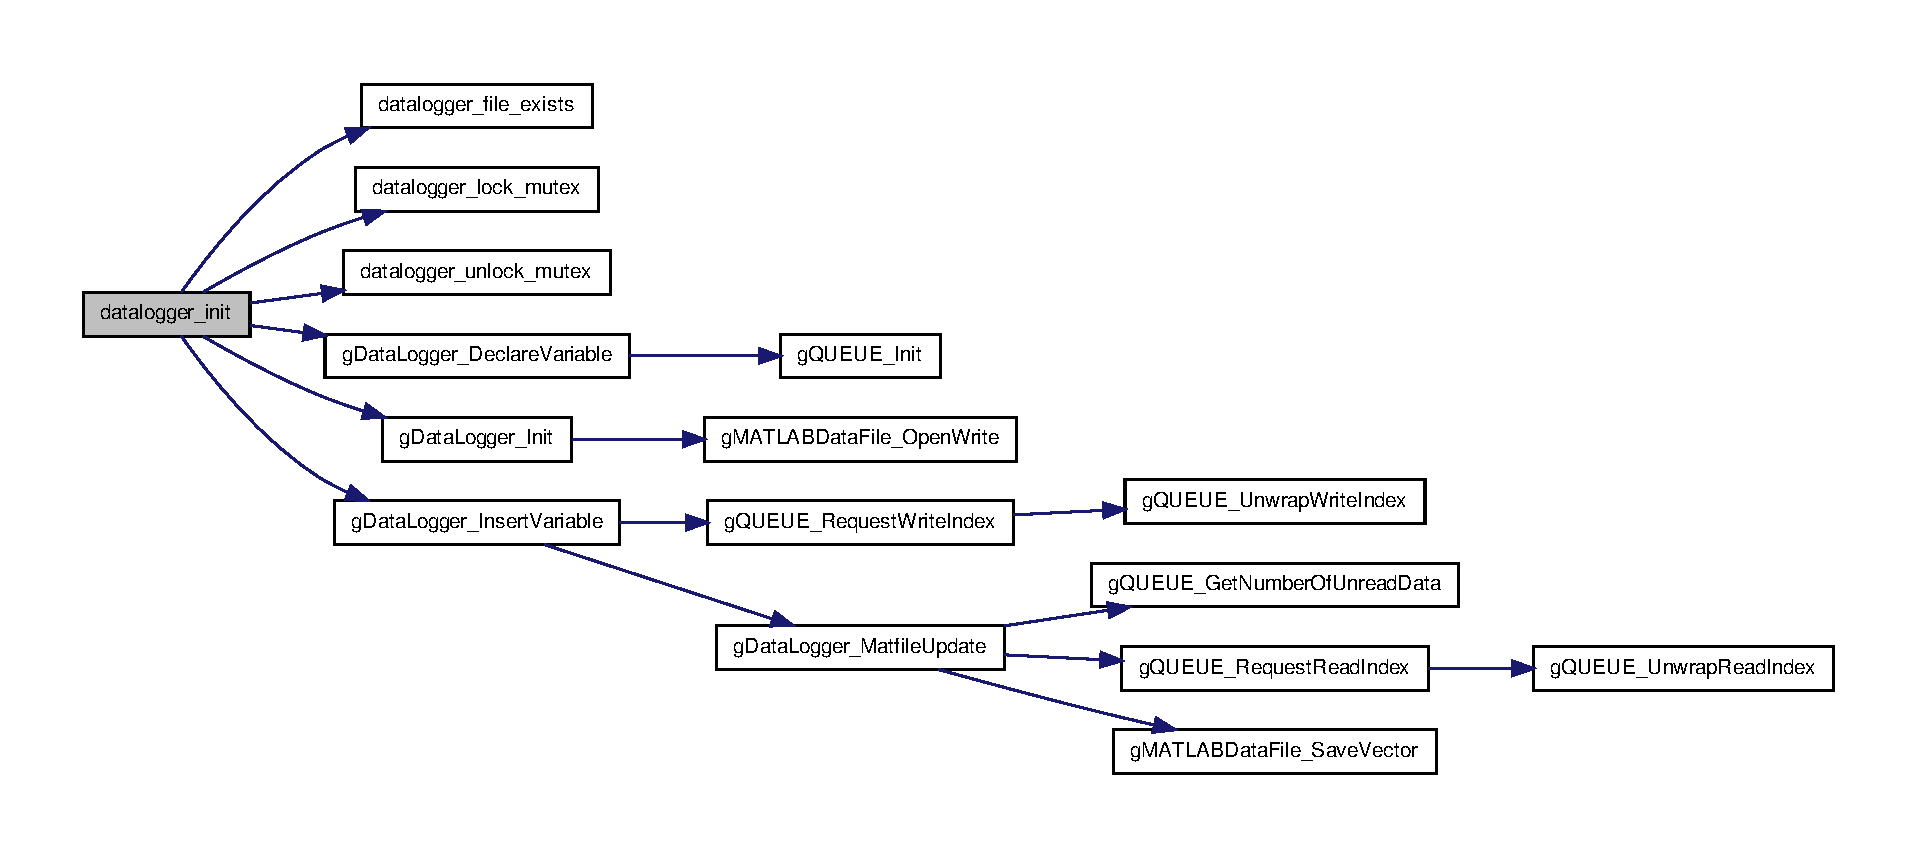
\includegraphics[width=350pt]{datalogger_8c_a1977ef253746fd8c008a3641d9822551_cgraph}
\end{center}
\end{figure}




Here is the caller graph for this function\-:\nopagebreak
\begin{figure}[H]
\begin{center}
\leavevmode
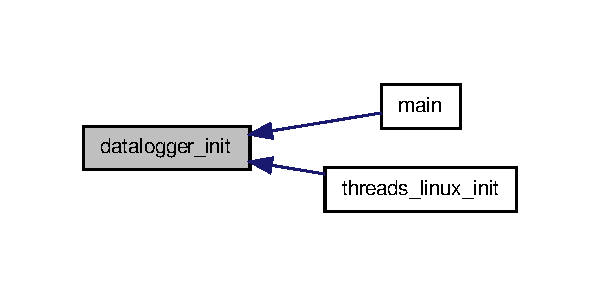
\includegraphics[width=288pt]{datalogger_8c_a1977ef253746fd8c008a3641d9822551_icgraph}
\end{center}
\end{figure}


\hypertarget{datalogger_8c_a54b06d9395b2e370a5a72beb7f9524b2}{\index{datalogger.\-c@{datalogger.\-c}!datalogger\-\_\-lock\-\_\-mutex@{datalogger\-\_\-lock\-\_\-mutex}}
\index{datalogger\-\_\-lock\-\_\-mutex@{datalogger\-\_\-lock\-\_\-mutex}!datalogger.c@{datalogger.\-c}}
\subsubsection[{datalogger\-\_\-lock\-\_\-mutex}]{\setlength{\rightskip}{0pt plus 5cm}int datalogger\-\_\-lock\-\_\-mutex (
\begin{DoxyParamCaption}
\item[{void}]{}
\end{DoxyParamCaption}
)}}\label{datalogger_8c_a54b06d9395b2e370a5a72beb7f9524b2}


Definition at line 629 of file datalogger.\-c.



References datalogger\-\_\-mutex, and D\-A\-T\-A\-L\-O\-G\-G\-E\-R\-\_\-\-S\-U\-C\-C\-E\-S\-S.



Referenced by datalogger\-\_\-close(), datalogger\-\_\-init(), datalogger\-\_\-set\-\_\-\-Ts(), datalogger\-\_\-start(), datalogger\-\_\-status(), datalogger\-\_\-stop(), datalogger\-\_\-update(), datalogger\-\_\-update\-\_\-\-I\-P\-C(), and datalogger\-\_\-write\-\_\-file().


\begin{DoxyCode}
\{
\textcolor{preprocessor}{        #if ANU\_COMPILE\_FOR\_XENOMAI}
\textcolor{preprocessor}{}        rt\_mutex\_acquire(&\hyperlink{datalogger_8c_a824d6f7fd1d3898ba0b1100ba37875c6}{datalogger\_mutex},TM\_INFINITE);
\textcolor{preprocessor}{        #else}
\textcolor{preprocessor}{}        pthread\_mutex\_lock(&\hyperlink{datalogger_8c_a824d6f7fd1d3898ba0b1100ba37875c6}{datalogger\_mutex});
\textcolor{preprocessor}{        #endif}
\textcolor{preprocessor}{}        \textcolor{keywordflow}{return} \hyperlink{datalogger_8h_abddebaf71d26d40183fccbb1a766b983}{DATALOGGER\_SUCCESS};
\}
\end{DoxyCode}


Here is the caller graph for this function\-:
\nopagebreak
\begin{figure}[H]
\begin{center}
\leavevmode
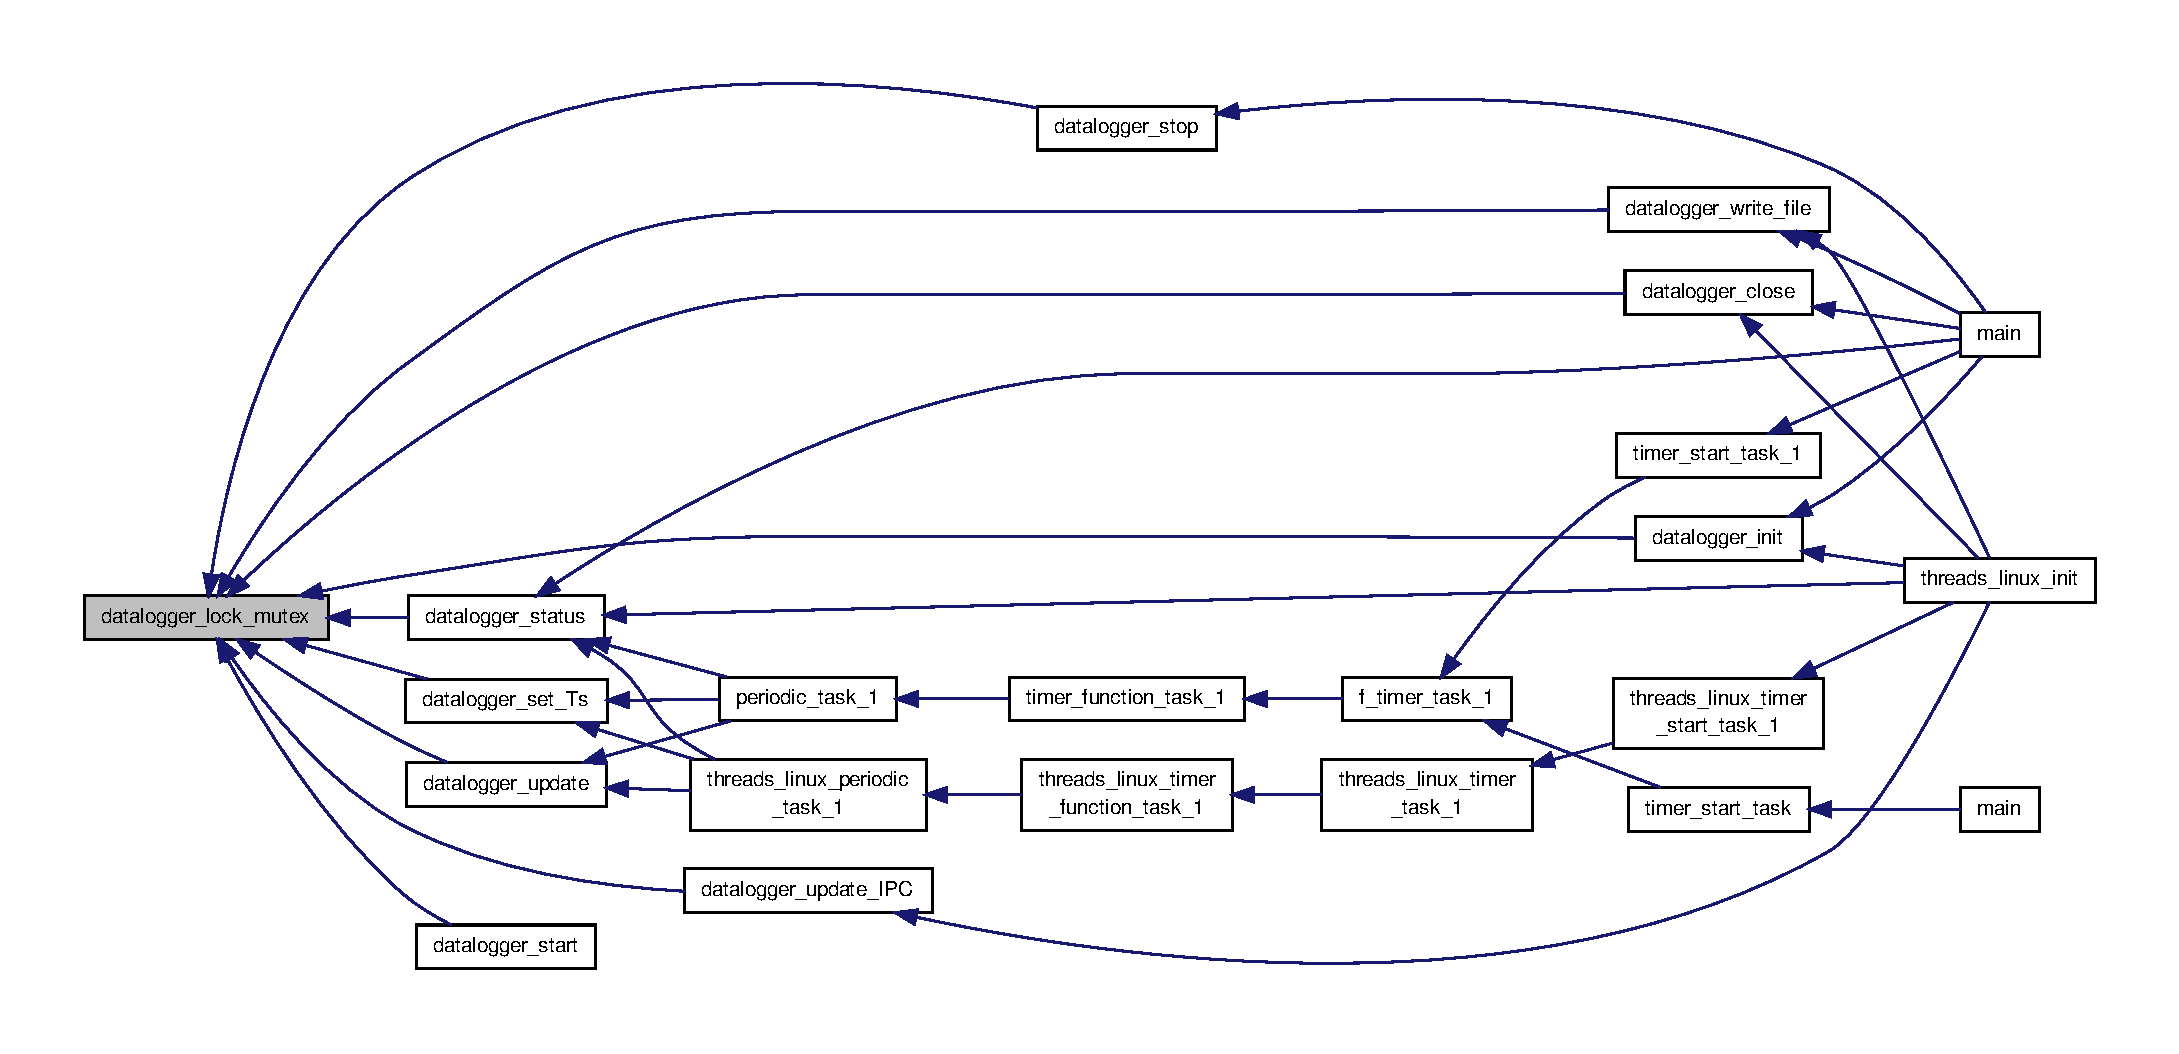
\includegraphics[width=350pt]{datalogger_8c_a54b06d9395b2e370a5a72beb7f9524b2_icgraph}
\end{center}
\end{figure}


\hypertarget{datalogger_8c_afb69d166f8d53042825174cee225ea49}{\index{datalogger.\-c@{datalogger.\-c}!datalogger\-\_\-set\-\_\-\-Ts@{datalogger\-\_\-set\-\_\-\-Ts}}
\index{datalogger\-\_\-set\-\_\-\-Ts@{datalogger\-\_\-set\-\_\-\-Ts}!datalogger.c@{datalogger.\-c}}
\subsubsection[{datalogger\-\_\-set\-\_\-\-Ts}]{\setlength{\rightskip}{0pt plus 5cm}int datalogger\-\_\-set\-\_\-\-Ts (
\begin{DoxyParamCaption}
\item[{double}]{Ts}
\end{DoxyParamCaption}
)}}\label{datalogger_8c_afb69d166f8d53042825174cee225ea49}


Definition at line 540 of file datalogger.\-c.



References D\-A\-T\-A\-L\-O\-G\-G\-E\-R\-\_\-\-E\-R\-R\-O\-R\-\_\-\-N\-O\-T\-\_\-\-I\-N\-I\-T\-I\-A\-L\-I\-Z\-E\-D, D\-A\-T\-A\-L\-O\-G\-G\-E\-R\-\_\-\-I\-N\-I\-T\-I\-A\-L\-I\-Z\-E\-D, datalogger\-\_\-initialized, datalogger\-\_\-lock\-\_\-mutex(), D\-A\-T\-A\-L\-O\-G\-G\-E\-R\-\_\-\-S\-U\-C\-C\-E\-S\-S, datalogger\-\_\-unlock\-\_\-mutex(), D\-A\-T\-A\-L\-O\-G\-G\-E\-R\-\_\-\-V\-A\-R\-I\-A\-B\-L\-E\-\_\-\-I\-N\-S\-E\-R\-T\-E\-D, D\-A\-T\-A\-L\-O\-G\-G\-E\-R\-\_\-\-V\-A\-R\-I\-A\-B\-L\-E\-\_\-\-N\-O\-T\-\_\-\-I\-N\-S\-E\-R\-T\-E\-D, D\-A\-T\-A\-L\-O\-G\-G\-E\-R\-\_\-\-V\-A\-R\-I\-B\-A\-L\-E\-\_\-\-A\-L\-R\-E\-A\-D\-Y\-\_\-\-I\-N\-S\-E\-R\-T\-E\-D, and g\-Data\-Logger\-\_\-\-Insert\-Variable().



Referenced by periodic\-\_\-task\-\_\-1(), and threads\-\_\-linux\-\_\-periodic\-\_\-task\-\_\-1().


\begin{DoxyCode}
\{
    \textcolor{keyword}{static} \textcolor{keywordtype}{int} datalogger\_Ts\_inserted = \hyperlink{datalogger_8h_a1f4fd2dbd981cf35467ab688c9157a74}{DATALOGGER\_VARIABLE\_NOT\_INSERTED}
      ;

    \hyperlink{datalogger_8c_a54b06d9395b2e370a5a72beb7f9524b2}{datalogger\_lock\_mutex}();

    \textcolor{keywordflow}{if}(\hyperlink{datalogger_8c_a35e8fbe04b90452afdc3c1be16ff6187}{datalogger\_initialized} != \hyperlink{datalogger_8h_a684c343d340004b77ca2b782934c96ca}{DATALOGGER\_INITIALIZED}
      )
    \{
        \hyperlink{datalogger_8c_a85453211c0c809083c36cc56b275aeeb}{datalogger\_unlock\_mutex}();
        \textcolor{keywordflow}{return} \hyperlink{datalogger_8h_a60df7fe0e61b757ad6a9db106b0eb43e}{DATALOGGER\_ERROR\_NOT\_INITIALIZED}
      ;
    \}

\textcolor{preprocessor}{    #if DATALOGGER\_LOG\_TIME}
\textcolor{preprocessor}{}    \textcolor{keywordflow}{if}(datalogger\_Ts\_inserted == \hyperlink{datalogger_8h_a1f4fd2dbd981cf35467ab688c9157a74}{DATALOGGER\_VARIABLE\_NOT\_INSERTED}
      )
    \{
        datalogger\_Ts\_inserted = \hyperlink{datalogger_8h_a181f9a0649abd26c74ed1a8a1710e25f}{DATALOGGER\_VARIABLE\_INSERTED}
      ;
        \hyperlink{gdatalogger_8c_a32674e7c2afa8b78e99a0070cf4bcaf9}{gDataLogger\_InsertVariable}(&\hyperlink{datalogger_8c_abe3b9c2c4e21e79c7b046b5986d13acc}{gDataLogger}
      , \textcolor{stringliteral}{"Ts"}, &Ts);
    \}
    \textcolor{keywordflow}{else}
        \{
        \hyperlink{datalogger_8c_a85453211c0c809083c36cc56b275aeeb}{datalogger\_unlock\_mutex}();
        \textcolor{keywordflow}{return} \hyperlink{datalogger_8h_ac76269a113d60c063e857d14e4a2f640}{DATALOGGER\_VARIBALE\_ALREADY\_INSERTED}
      ;
        \}
\textcolor{preprocessor}{    #else}
\textcolor{preprocessor}{}    \textcolor{keywordtype}{double} tmp = Ts; \textcolor{comment}{// Remove warning}
\textcolor{preprocessor}{    #endif // DATALOGGER\_LOG\_TIME}
\textcolor{preprocessor}{}
    \hyperlink{datalogger_8c_a85453211c0c809083c36cc56b275aeeb}{datalogger\_unlock\_mutex}();
    \textcolor{keywordflow}{return} \hyperlink{datalogger_8h_abddebaf71d26d40183fccbb1a766b983}{DATALOGGER\_SUCCESS};
\}
\end{DoxyCode}


Here is the call graph for this function\-:\nopagebreak
\begin{figure}[H]
\begin{center}
\leavevmode
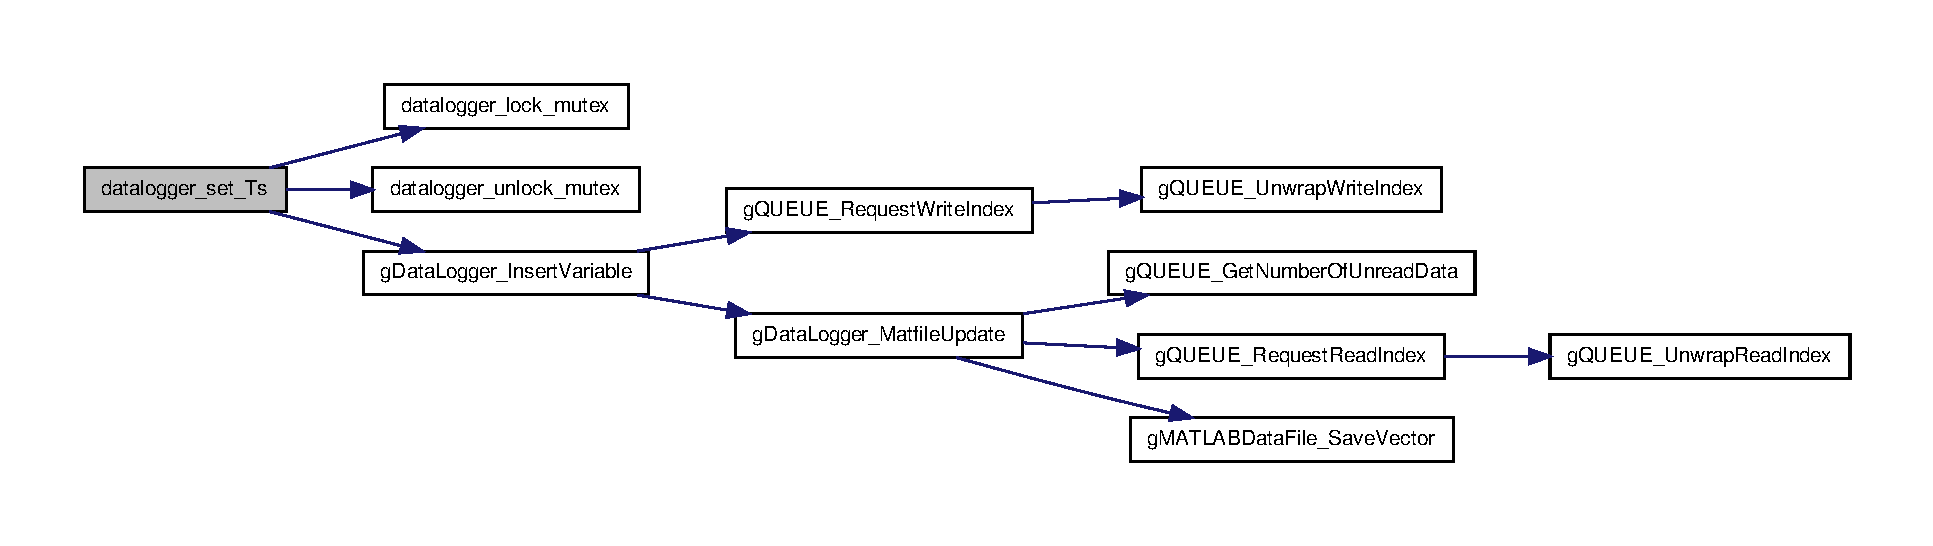
\includegraphics[width=350pt]{datalogger_8c_afb69d166f8d53042825174cee225ea49_cgraph}
\end{center}
\end{figure}




Here is the caller graph for this function\-:\nopagebreak
\begin{figure}[H]
\begin{center}
\leavevmode
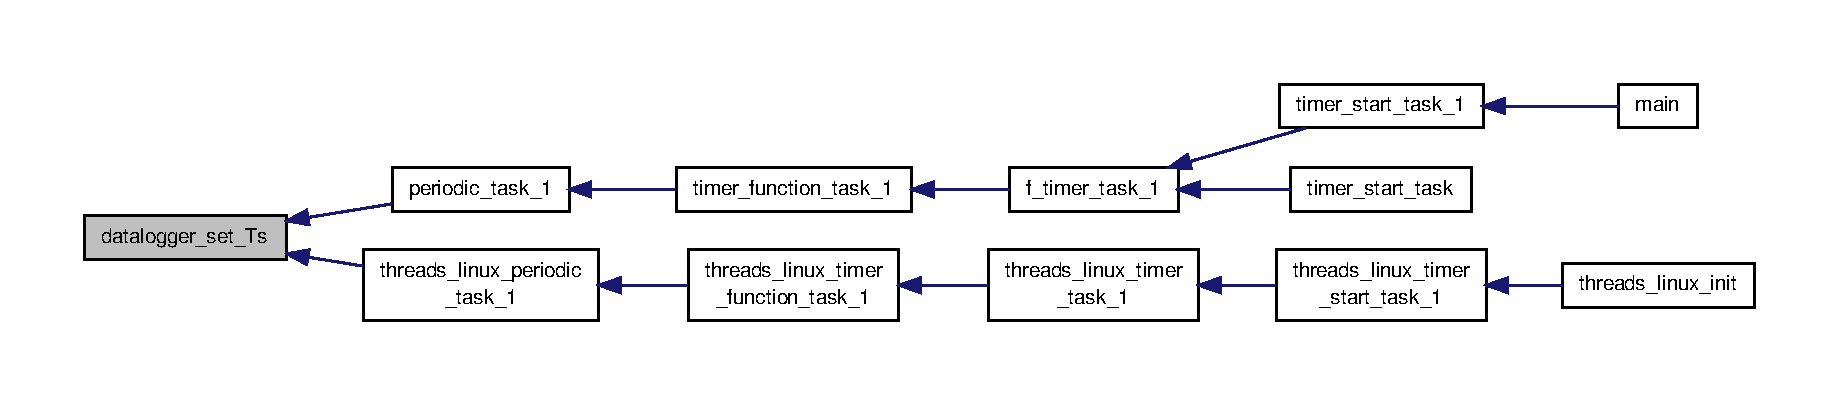
\includegraphics[width=350pt]{datalogger_8c_afb69d166f8d53042825174cee225ea49_icgraph}
\end{center}
\end{figure}


\hypertarget{datalogger_8c_a1f254ef380d595d6605c10811fd0dee6}{\index{datalogger.\-c@{datalogger.\-c}!datalogger\-\_\-start@{datalogger\-\_\-start}}
\index{datalogger\-\_\-start@{datalogger\-\_\-start}!datalogger.c@{datalogger.\-c}}
\subsubsection[{datalogger\-\_\-start}]{\setlength{\rightskip}{0pt plus 5cm}int datalogger\-\_\-start (
\begin{DoxyParamCaption}
\item[{void}]{}
\end{DoxyParamCaption}
)}}\label{datalogger_8c_a1f254ef380d595d6605c10811fd0dee6}


Definition at line 584 of file datalogger.\-c.



References D\-A\-T\-A\-L\-O\-G\-G\-E\-R\-\_\-\-E\-R\-R\-O\-R\-\_\-\-N\-O\-T\-\_\-\-I\-N\-I\-T\-I\-A\-L\-I\-Z\-E\-D, D\-A\-T\-A\-L\-O\-G\-G\-E\-R\-\_\-\-I\-N\-I\-T\-I\-A\-L\-I\-Z\-E\-D, datalogger\-\_\-initialized, datalogger\-\_\-lock\-\_\-mutex(), datalogger\-\_\-running, D\-A\-T\-A\-L\-O\-G\-G\-E\-R\-\_\-\-R\-U\-N\-N\-I\-N\-G, D\-A\-T\-A\-L\-O\-G\-G\-E\-R\-\_\-\-S\-U\-C\-C\-E\-S\-S, and datalogger\-\_\-unlock\-\_\-mutex().



Referenced by ui\-\_\-update().


\begin{DoxyCode}
\{
\textcolor{preprocessor}{    #if DATALOGGER\_MODULE\_ENABLED}
\textcolor{preprocessor}{}    \hyperlink{datalogger_8c_a54b06d9395b2e370a5a72beb7f9524b2}{datalogger\_lock\_mutex}();
    \textcolor{keywordflow}{if}(\hyperlink{datalogger_8c_a35e8fbe04b90452afdc3c1be16ff6187}{datalogger\_initialized} != \hyperlink{datalogger_8h_a684c343d340004b77ca2b782934c96ca}{DATALOGGER\_INITIALIZED}
      )
    \{
        \hyperlink{datalogger_8c_a85453211c0c809083c36cc56b275aeeb}{datalogger\_unlock\_mutex}();
        \textcolor{keywordflow}{return} \hyperlink{datalogger_8h_a60df7fe0e61b757ad6a9db106b0eb43e}{DATALOGGER\_ERROR\_NOT\_INITIALIZED}
      ;
    \}

    \hyperlink{datalogger_8c_a185c3ede96449d14f330fe5ac664e799}{datalogger\_running} = \hyperlink{datalogger_8h_a2cf92051a019c8ec1b5c4f5380758f62}{DATALOGGER\_RUNNING}
      ;
    \hyperlink{datalogger_8c_a85453211c0c809083c36cc56b275aeeb}{datalogger\_unlock\_mutex}();
\textcolor{preprocessor}{    #endif}
\textcolor{preprocessor}{}
    \textcolor{keywordflow}{return} \hyperlink{datalogger_8h_abddebaf71d26d40183fccbb1a766b983}{DATALOGGER\_SUCCESS};
\}
\end{DoxyCode}


Here is the call graph for this function\-:\nopagebreak
\begin{figure}[H]
\begin{center}
\leavevmode
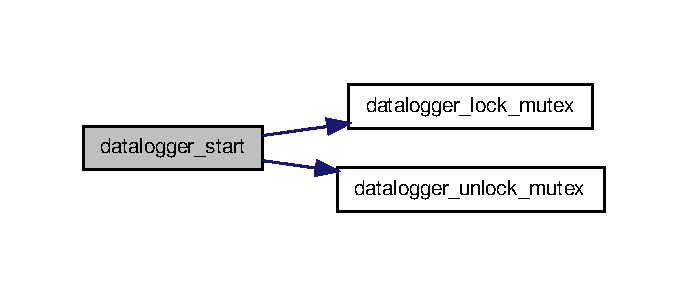
\includegraphics[width=330pt]{datalogger_8c_a1f254ef380d595d6605c10811fd0dee6_cgraph}
\end{center}
\end{figure}




Here is the caller graph for this function\-:
\nopagebreak
\begin{figure}[H]
\begin{center}
\leavevmode
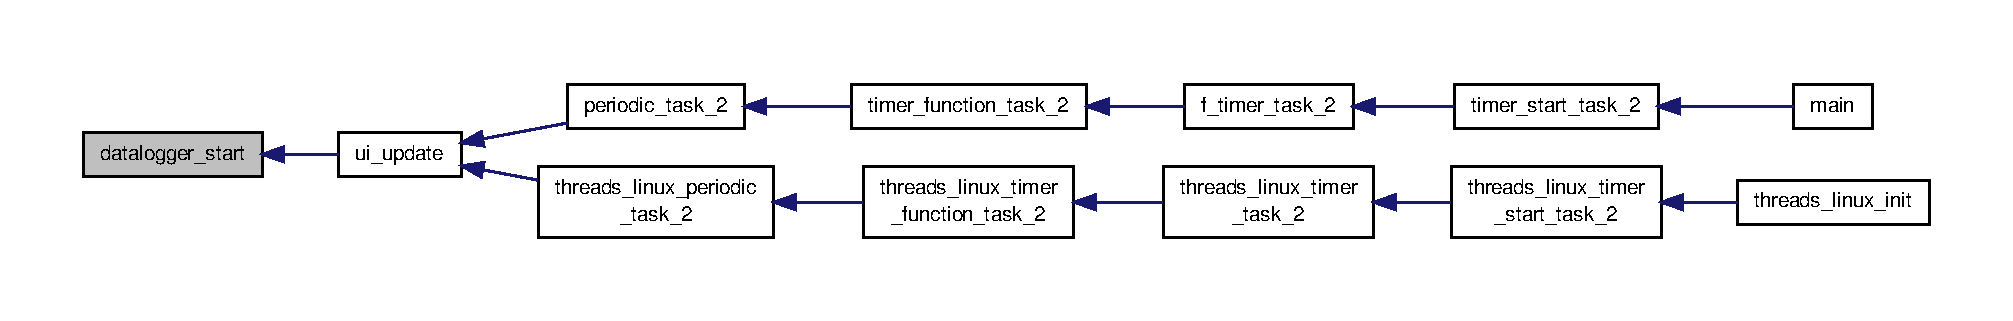
\includegraphics[width=350pt]{datalogger_8c_a1f254ef380d595d6605c10811fd0dee6_icgraph}
\end{center}
\end{figure}


\hypertarget{datalogger_8c_a46fd1290d9ee97d5fc7171e1e0dcb0aa}{\index{datalogger.\-c@{datalogger.\-c}!datalogger\-\_\-status@{datalogger\-\_\-status}}
\index{datalogger\-\_\-status@{datalogger\-\_\-status}!datalogger.c@{datalogger.\-c}}
\subsubsection[{datalogger\-\_\-status}]{\setlength{\rightskip}{0pt plus 5cm}int datalogger\-\_\-status (
\begin{DoxyParamCaption}
\item[{void}]{}
\end{DoxyParamCaption}
)}}\label{datalogger_8c_a46fd1290d9ee97d5fc7171e1e0dcb0aa}


Definition at line 571 of file datalogger.\-c.



References D\-A\-T\-A\-L\-O\-G\-G\-E\-R\-\_\-\-E\-R\-R\-O\-R\-\_\-\-N\-O\-T\-\_\-\-I\-N\-I\-T\-I\-A\-L\-I\-Z\-E\-D, D\-A\-T\-A\-L\-O\-G\-G\-E\-R\-\_\-\-I\-N\-I\-T\-I\-A\-L\-I\-Z\-E\-D, datalogger\-\_\-initialized, datalogger\-\_\-lock\-\_\-mutex(), datalogger\-\_\-running, and datalogger\-\_\-unlock\-\_\-mutex().



Referenced by main(), periodic\-\_\-task\-\_\-1(), threads\-\_\-linux\-\_\-init(), threads\-\_\-linux\-\_\-periodic\-\_\-task\-\_\-1(), ui\-\_\-overview\-\_\-data(), and ui\-\_\-update().


\begin{DoxyCode}
\{
    \hyperlink{datalogger_8c_a54b06d9395b2e370a5a72beb7f9524b2}{datalogger\_lock\_mutex}();
    \textcolor{keywordflow}{if}(\hyperlink{datalogger_8c_a35e8fbe04b90452afdc3c1be16ff6187}{datalogger\_initialized} != \hyperlink{datalogger_8h_a684c343d340004b77ca2b782934c96ca}{DATALOGGER\_INITIALIZED}
      )
    \{
        \hyperlink{datalogger_8c_a85453211c0c809083c36cc56b275aeeb}{datalogger\_unlock\_mutex}();
        \textcolor{keywordflow}{return} \hyperlink{datalogger_8h_a60df7fe0e61b757ad6a9db106b0eb43e}{DATALOGGER\_ERROR\_NOT\_INITIALIZED}
      ;
    \}

    \hyperlink{datalogger_8c_a85453211c0c809083c36cc56b275aeeb}{datalogger\_unlock\_mutex}();
    \textcolor{keywordflow}{return} \hyperlink{datalogger_8c_a185c3ede96449d14f330fe5ac664e799}{datalogger\_running};
\}
\end{DoxyCode}


Here is the call graph for this function\-:\nopagebreak
\begin{figure}[H]
\begin{center}
\leavevmode
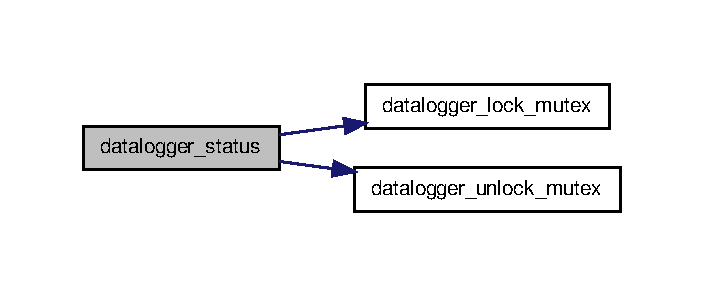
\includegraphics[width=338pt]{datalogger_8c_a46fd1290d9ee97d5fc7171e1e0dcb0aa_cgraph}
\end{center}
\end{figure}




Here is the caller graph for this function\-:
\nopagebreak
\begin{figure}[H]
\begin{center}
\leavevmode
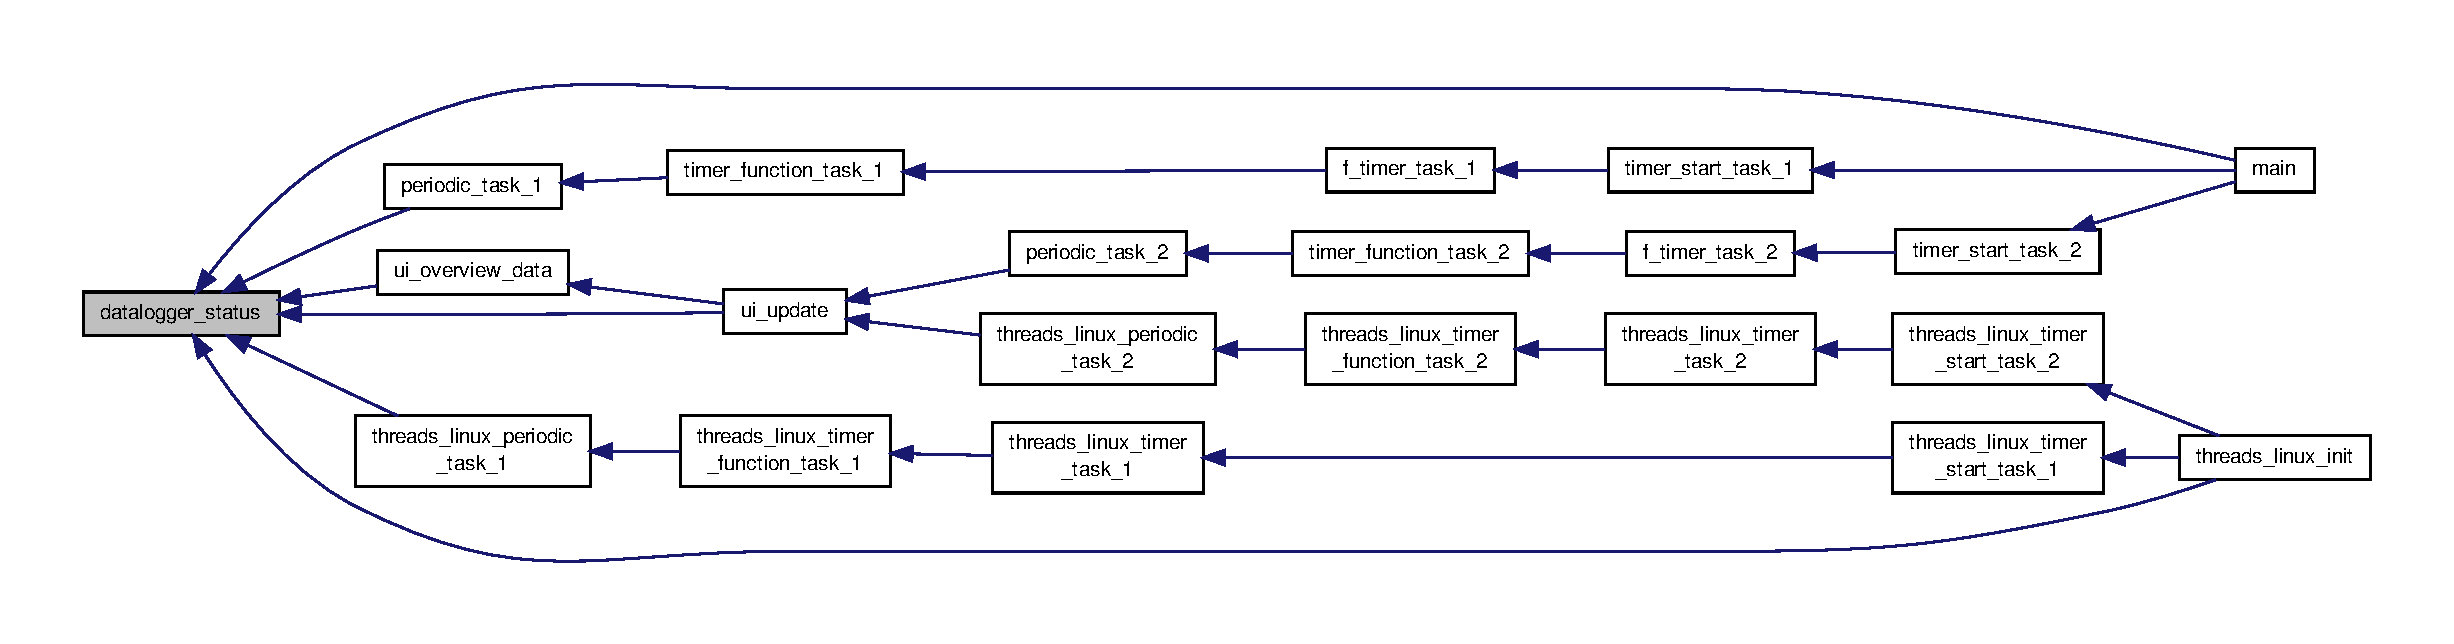
\includegraphics[width=350pt]{datalogger_8c_a46fd1290d9ee97d5fc7171e1e0dcb0aa_icgraph}
\end{center}
\end{figure}


\hypertarget{datalogger_8c_aae2ffbc6cbf8f1cfecceb42c5139530a}{\index{datalogger.\-c@{datalogger.\-c}!datalogger\-\_\-stop@{datalogger\-\_\-stop}}
\index{datalogger\-\_\-stop@{datalogger\-\_\-stop}!datalogger.c@{datalogger.\-c}}
\subsubsection[{datalogger\-\_\-stop}]{\setlength{\rightskip}{0pt plus 5cm}int datalogger\-\_\-stop (
\begin{DoxyParamCaption}
\item[{void}]{}
\end{DoxyParamCaption}
)}}\label{datalogger_8c_aae2ffbc6cbf8f1cfecceb42c5139530a}


Definition at line 601 of file datalogger.\-c.



References D\-A\-T\-A\-L\-O\-G\-G\-E\-R\-\_\-\-E\-R\-R\-O\-R\-\_\-\-N\-O\-T\-\_\-\-I\-N\-I\-T\-I\-A\-L\-I\-Z\-E\-D, D\-A\-T\-A\-L\-O\-G\-G\-E\-R\-\_\-\-I\-N\-I\-T\-I\-A\-L\-I\-Z\-E\-D, datalogger\-\_\-initialized, datalogger\-\_\-lock\-\_\-mutex(), D\-A\-T\-A\-L\-O\-G\-G\-E\-R\-\_\-\-N\-O\-T\-\_\-\-R\-U\-N\-N\-I\-N\-G, datalogger\-\_\-running, D\-A\-T\-A\-L\-O\-G\-G\-E\-R\-\_\-\-S\-U\-C\-C\-E\-S\-S, and datalogger\-\_\-unlock\-\_\-mutex().



Referenced by main(), and ui\-\_\-update().


\begin{DoxyCode}
\{
\textcolor{preprocessor}{    #if DATALOGGER\_MODULE\_ENABLED}
\textcolor{preprocessor}{}    \hyperlink{datalogger_8c_a54b06d9395b2e370a5a72beb7f9524b2}{datalogger\_lock\_mutex}();
    \textcolor{keywordflow}{if}(\hyperlink{datalogger_8c_a35e8fbe04b90452afdc3c1be16ff6187}{datalogger\_initialized} != \hyperlink{datalogger_8h_a684c343d340004b77ca2b782934c96ca}{DATALOGGER\_INITIALIZED}
      )
    \{
        \hyperlink{datalogger_8c_a85453211c0c809083c36cc56b275aeeb}{datalogger\_unlock\_mutex}();
        \textcolor{keywordflow}{return} \hyperlink{datalogger_8h_a60df7fe0e61b757ad6a9db106b0eb43e}{DATALOGGER\_ERROR\_NOT\_INITIALIZED}
      ;
    \}

    \hyperlink{datalogger_8c_a185c3ede96449d14f330fe5ac664e799}{datalogger\_running} = \hyperlink{datalogger_8h_a1a224da36800f52f56f30619849f7f5d}{DATALOGGER\_NOT\_RUNNING}
      ;
    \hyperlink{datalogger_8c_a85453211c0c809083c36cc56b275aeeb}{datalogger\_unlock\_mutex}();
\textcolor{preprocessor}{    #endif}
\textcolor{preprocessor}{}
    \textcolor{keywordflow}{return} \hyperlink{datalogger_8h_abddebaf71d26d40183fccbb1a766b983}{DATALOGGER\_SUCCESS};
\}
\end{DoxyCode}


Here is the call graph for this function\-:\nopagebreak
\begin{figure}[H]
\begin{center}
\leavevmode
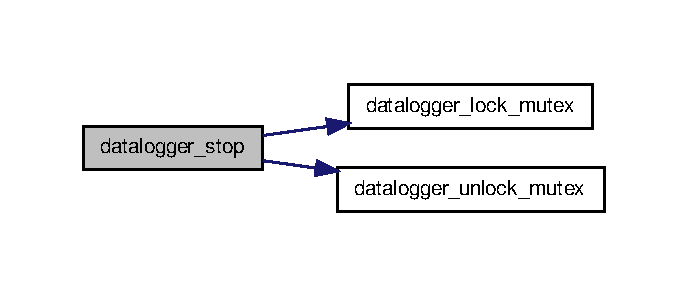
\includegraphics[width=330pt]{datalogger_8c_aae2ffbc6cbf8f1cfecceb42c5139530a_cgraph}
\end{center}
\end{figure}




Here is the caller graph for this function\-:
\nopagebreak
\begin{figure}[H]
\begin{center}
\leavevmode
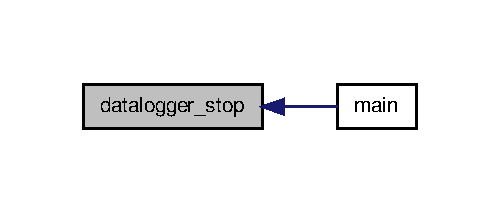
\includegraphics[width=350pt]{datalogger_8c_aae2ffbc6cbf8f1cfecceb42c5139530a_icgraph}
\end{center}
\end{figure}


\hypertarget{datalogger_8c_a85453211c0c809083c36cc56b275aeeb}{\index{datalogger.\-c@{datalogger.\-c}!datalogger\-\_\-unlock\-\_\-mutex@{datalogger\-\_\-unlock\-\_\-mutex}}
\index{datalogger\-\_\-unlock\-\_\-mutex@{datalogger\-\_\-unlock\-\_\-mutex}!datalogger.c@{datalogger.\-c}}
\subsubsection[{datalogger\-\_\-unlock\-\_\-mutex}]{\setlength{\rightskip}{0pt plus 5cm}int datalogger\-\_\-unlock\-\_\-mutex (
\begin{DoxyParamCaption}
\item[{void}]{}
\end{DoxyParamCaption}
)}}\label{datalogger_8c_a85453211c0c809083c36cc56b275aeeb}


Definition at line 639 of file datalogger.\-c.



References datalogger\-\_\-mutex, and D\-A\-T\-A\-L\-O\-G\-G\-E\-R\-\_\-\-S\-U\-C\-C\-E\-S\-S.



Referenced by datalogger\-\_\-close(), datalogger\-\_\-init(), datalogger\-\_\-set\-\_\-\-Ts(), datalogger\-\_\-start(), datalogger\-\_\-status(), datalogger\-\_\-stop(), datalogger\-\_\-update(), datalogger\-\_\-update\-\_\-\-I\-P\-C(), and datalogger\-\_\-write\-\_\-file().


\begin{DoxyCode}
\{
\textcolor{preprocessor}{        #if ANU\_COMPILE\_FOR\_XENOMAI}
\textcolor{preprocessor}{}        rt\_mutex\_release(&\hyperlink{datalogger_8c_a824d6f7fd1d3898ba0b1100ba37875c6}{datalogger\_mutex});
\textcolor{preprocessor}{        #else}
\textcolor{preprocessor}{}        pthread\_mutex\_unlock(&\hyperlink{datalogger_8c_a824d6f7fd1d3898ba0b1100ba37875c6}{datalogger\_mutex});
\textcolor{preprocessor}{        #endif}
\textcolor{preprocessor}{}        \textcolor{keywordflow}{return} \hyperlink{datalogger_8h_abddebaf71d26d40183fccbb1a766b983}{DATALOGGER\_SUCCESS};
\}
\end{DoxyCode}


Here is the caller graph for this function\-:
\nopagebreak
\begin{figure}[H]
\begin{center}
\leavevmode
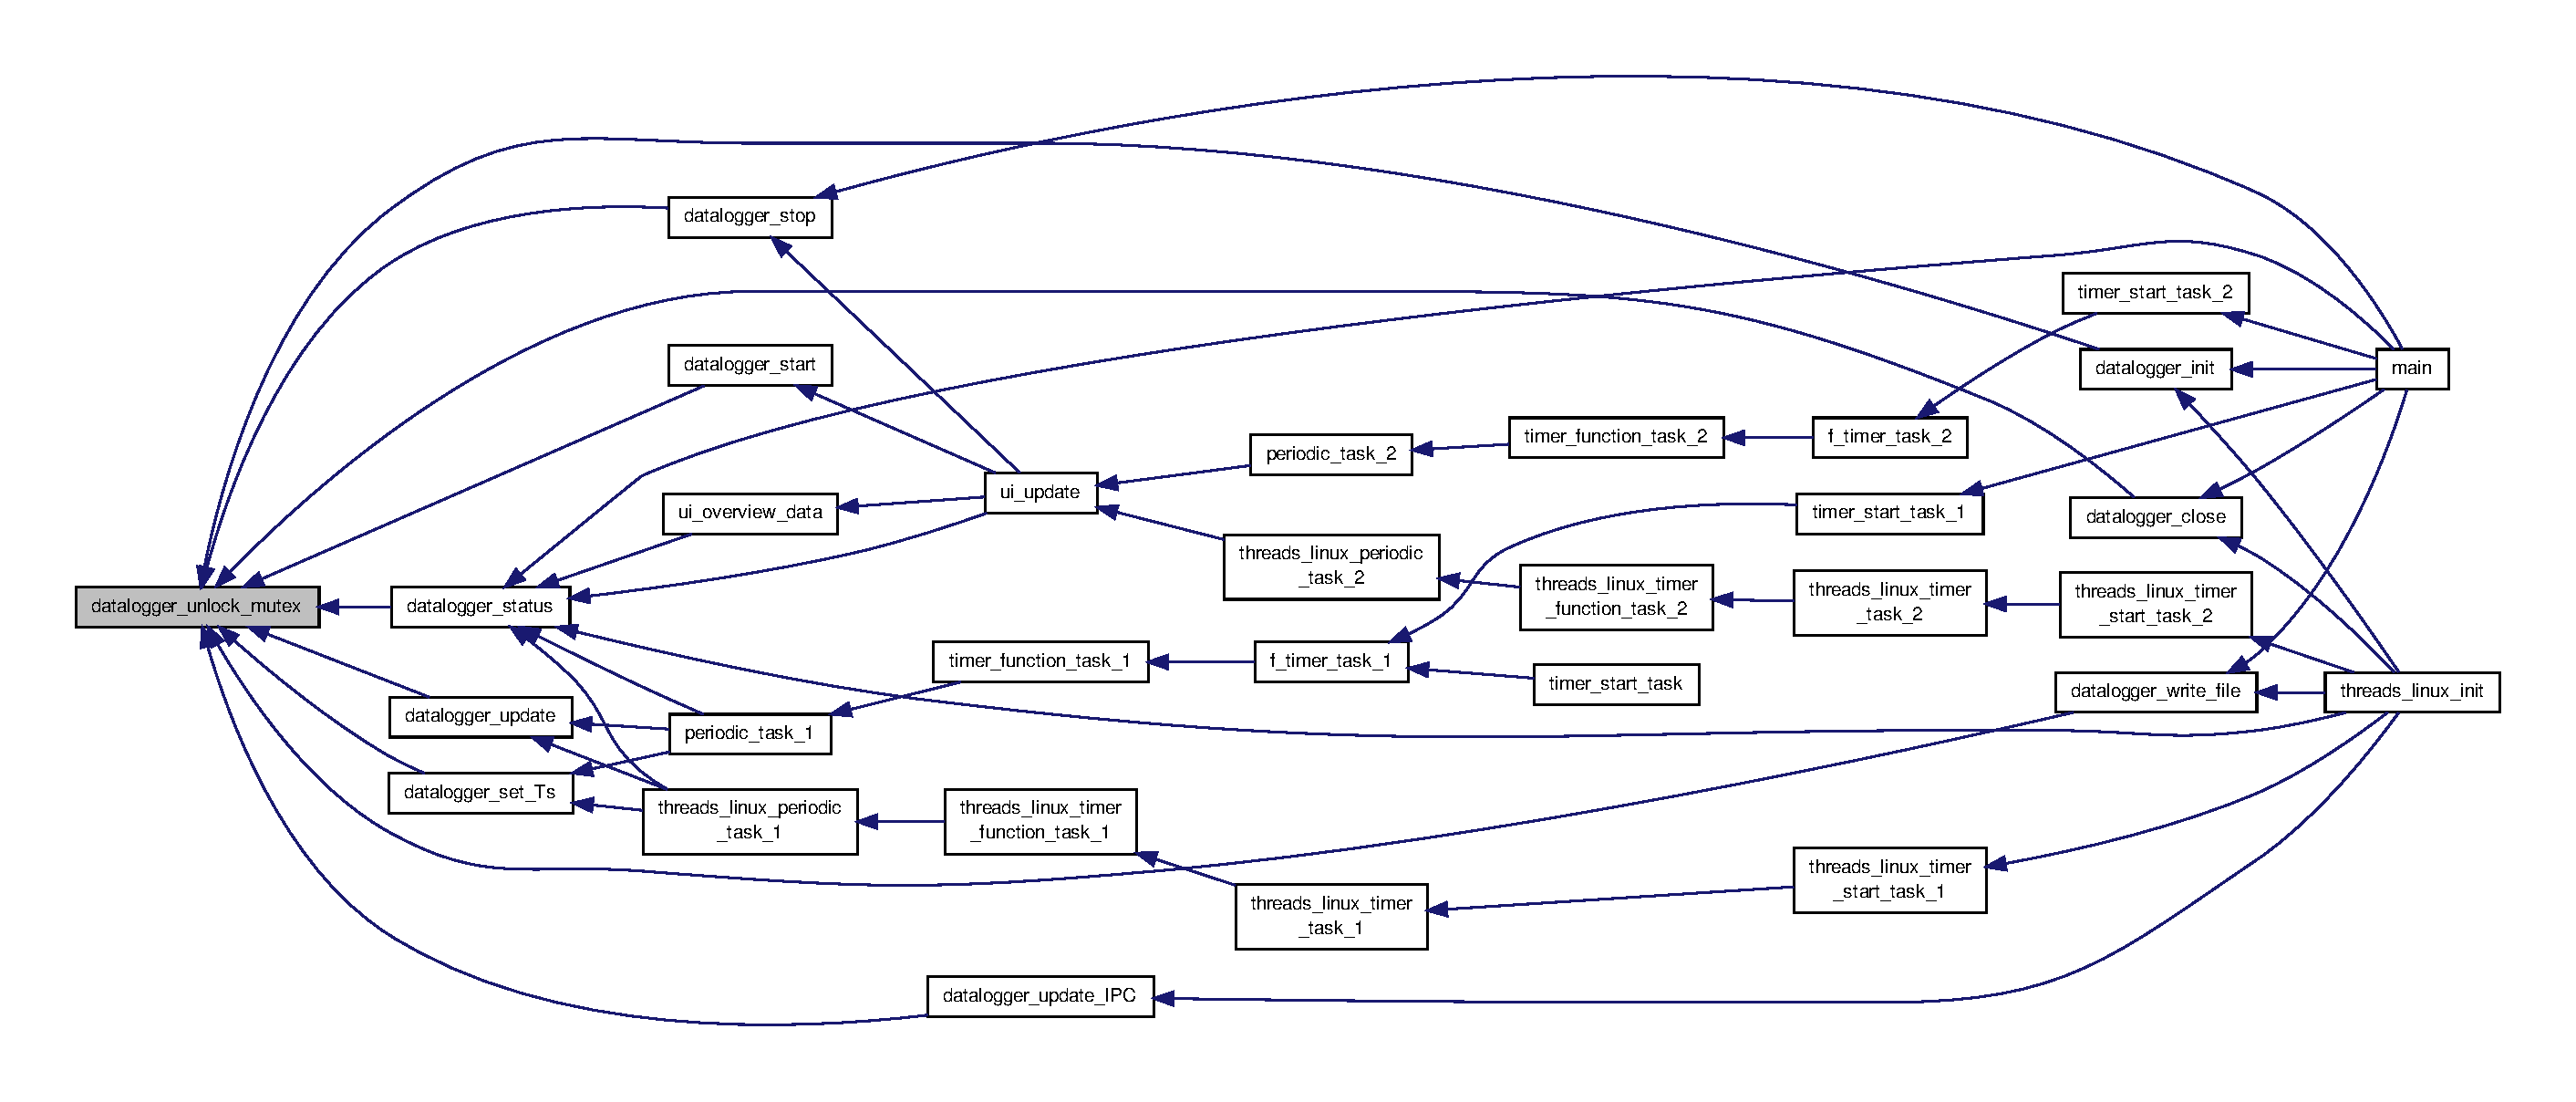
\includegraphics[width=350pt]{datalogger_8c_a85453211c0c809083c36cc56b275aeeb_icgraph}
\end{center}
\end{figure}


\hypertarget{datalogger_8c_ad89a56e2f057ace8c28d78eb67703e7d}{\index{datalogger.\-c@{datalogger.\-c}!datalogger\-\_\-update@{datalogger\-\_\-update}}
\index{datalogger\-\_\-update@{datalogger\-\_\-update}!datalogger.c@{datalogger.\-c}}
\subsubsection[{datalogger\-\_\-update}]{\setlength{\rightskip}{0pt plus 5cm}int datalogger\-\_\-update (
\begin{DoxyParamCaption}
\item[{double}]{t\-\_\-s, }
\item[{double}]{t\-\_\-control\-\_\-exec\-\_\-s, }
\item[{double}]{t\-\_\-ui\-\_\-exec\-\_\-s, }
\item[{double}]{t0\-\_\-s, }
\item[{{\bf I\-M\-U\-\_\-\-D\-A\-T\-A\-\_\-\-S\-T\-R\-U\-C\-T} $\ast$}]{pimu\-\_\-data, }
\item[{{\bf E\-F\-F\-\_\-\-D\-A\-T\-A\-\_\-\-S\-T\-R\-U\-C\-T} $\ast$}]{peff\-\_\-data, }
\item[{{\bf M\-R\-A\-\_\-\-D\-A\-T\-A\-\_\-\-S\-T\-R\-U\-C\-T} $\ast$}]{pmra\-\_\-data}
\end{DoxyParamCaption}
)}}\label{datalogger_8c_ad89a56e2f057ace8c28d78eb67703e7d}


Definition at line 272 of file datalogger.\-c.



References I\-M\-U\-\_\-\-D\-A\-T\-A\-\_\-\-S\-T\-R\-U\-C\-T\-::acc, I\-M\-U\-\_\-\-D\-A\-T\-A\-\_\-\-S\-T\-R\-U\-C\-T\-::calibrated\-::acc, I\-M\-U\-\_\-\-D\-A\-T\-A\-\_\-\-S\-T\-R\-U\-C\-T\-::calib, D\-A\-T\-A\-L\-O\-G\-G\-E\-R\-\_\-\-E\-R\-R\-O\-R\-\_\-\-N\-O\-T\-\_\-\-I\-N\-I\-T\-I\-A\-L\-I\-Z\-E\-D, D\-A\-T\-A\-L\-O\-G\-G\-E\-R\-\_\-\-I\-N\-I\-T\-I\-A\-L\-I\-Z\-E\-D, datalogger\-\_\-initialized, datalogger\-\_\-lock\-\_\-mutex(), D\-A\-T\-A\-L\-O\-G\-G\-E\-R\-\_\-\-S\-U\-C\-C\-E\-S\-S, datalogger\-\_\-unlock\-\_\-mutex(), E\-F\-F\-\_\-\-D\-A\-T\-A\-\_\-\-S\-T\-R\-U\-C\-T\-::\-F, g\-Data\-Logger\-\_\-\-Insert\-Variable(), I\-M\-U\-\_\-\-D\-A\-T\-A\-\_\-\-S\-T\-R\-U\-C\-T\-::gyr, I\-M\-U\-\_\-\-D\-A\-T\-A\-\_\-\-S\-T\-R\-U\-C\-T\-::calibrated\-::gyr, I\-M\-U\-\_\-\-D\-A\-T\-A\-\_\-\-S\-T\-R\-U\-C\-T\-::mag, I\-M\-U\-\_\-\-D\-A\-T\-A\-\_\-\-S\-T\-R\-U\-C\-T\-::calibrated\-::mag, I\-M\-U\-\_\-\-D\-A\-T\-A\-\_\-\-S\-T\-R\-U\-C\-T\-::new\-\_\-data, E\-F\-F\-\_\-\-D\-A\-T\-A\-\_\-\-S\-T\-R\-U\-C\-T\-::new\-\_\-data, M\-R\-A\-\_\-\-D\-A\-T\-A\-\_\-\-S\-T\-R\-U\-C\-T\-::v\-\_\-ctl, M\-R\-A\-\_\-\-D\-A\-T\-A\-\_\-\-S\-T\-R\-U\-C\-T\-::v\-\_\-ctl\-\_\-read, D\-A\-T\-A\-\_\-\-X\-Y\-Z\-::x, D\-A\-T\-A\-\_\-\-X\-Y\-Z\-\_\-\-D\-O\-U\-B\-L\-E\-::x, D\-A\-T\-A\-\_\-\-X\-Y\-Z\-::y, D\-A\-T\-A\-\_\-\-X\-Y\-Z\-\_\-\-D\-O\-U\-B\-L\-E\-::y, D\-A\-T\-A\-\_\-\-X\-Y\-Z\-::z, and D\-A\-T\-A\-\_\-\-X\-Y\-Z\-\_\-\-D\-O\-U\-B\-L\-E\-::z.



Referenced by periodic\-\_\-task\-\_\-1(), and threads\-\_\-linux\-\_\-periodic\-\_\-task\-\_\-1().


\begin{DoxyCode}
\{
    \textcolor{keywordtype}{double} tmp = 0.0;

    \hyperlink{datalogger_8c_a54b06d9395b2e370a5a72beb7f9524b2}{datalogger\_lock\_mutex}();

    \textcolor{keywordflow}{if}(\hyperlink{datalogger_8c_a35e8fbe04b90452afdc3c1be16ff6187}{datalogger\_initialized} != \hyperlink{datalogger_8h_a684c343d340004b77ca2b782934c96ca}{DATALOGGER\_INITIALIZED}
      )
    \{
        \hyperlink{datalogger_8c_a85453211c0c809083c36cc56b275aeeb}{datalogger\_unlock\_mutex}();
        \textcolor{keywordflow}{return} \hyperlink{datalogger_8h_a60df7fe0e61b757ad6a9db106b0eb43e}{DATALOGGER\_ERROR\_NOT\_INITIALIZED}
      ;
    \}

\textcolor{preprocessor}{    #if DATALOGGER\_LOG\_TIME}
\textcolor{preprocessor}{}    \textcolor{keywordtype}{double} tmp\_t = t\_s - t0\_s;
    \hyperlink{gdatalogger_8c_a32674e7c2afa8b78e99a0070cf4bcaf9}{gDataLogger\_InsertVariable}(&\hyperlink{datalogger_8c_abe3b9c2c4e21e79c7b046b5986d13acc}{gDataLogger}
      , \textcolor{stringliteral}{"t"}, &tmp\_t);
\textcolor{preprocessor}{    #else}
\textcolor{preprocessor}{}    \textcolor{keywordtype}{double} tmp\_t = 0.0;
    tmp\_t = t\_s; \textcolor{comment}{// Remove warning}
\textcolor{preprocessor}{    #endif // DATALOGGER\_LOG\_TIME}
\textcolor{preprocessor}{}
\textcolor{preprocessor}{    #if DATALOGGER\_LOG\_EXECTIMES}
\textcolor{preprocessor}{}    \hyperlink{gdatalogger_8c_a32674e7c2afa8b78e99a0070cf4bcaf9}{gDataLogger\_InsertVariable}(&\hyperlink{datalogger_8c_abe3b9c2c4e21e79c7b046b5986d13acc}{gDataLogger}
      , \textcolor{stringliteral}{"t\_control\_exec"}, &t\_control\_exec\_s);
    \hyperlink{gdatalogger_8c_a32674e7c2afa8b78e99a0070cf4bcaf9}{gDataLogger\_InsertVariable}(&\hyperlink{datalogger_8c_abe3b9c2c4e21e79c7b046b5986d13acc}{gDataLogger}
      , \textcolor{stringliteral}{"t\_ui\_exec"}, &t\_ui\_exec\_s);
\textcolor{preprocessor}{    #else}
\textcolor{preprocessor}{}    \textcolor{keywordtype}{double} tmp\_e = 0.0; \textcolor{comment}{// Remove warning}
    tmp\_e = t\_control\_exec\_s; \textcolor{comment}{// Remove warning}
    tmp\_e = t\_ui\_exec\_s; \textcolor{comment}{// Remove warning}
\textcolor{preprocessor}{    #endif // DATALOGGER\_LOG\_EXECTIMES}
\textcolor{preprocessor}{}

\textcolor{preprocessor}{    #if DATALOGGER\_LOG\_RAW\_IMU}
\textcolor{preprocessor}{}    tmp = (double) pimu\_data->\hyperlink{structIMU__DATA__STRUCT_a448f284bf44eb503affda586ad5fa9d2}{acc}.\hyperlink{structDATA__XYZ_a54c1596e9f9969fd9c21e8458024ecfb}{x};
    \hyperlink{gdatalogger_8c_a32674e7c2afa8b78e99a0070cf4bcaf9}{gDataLogger\_InsertVariable}(&\hyperlink{datalogger_8c_abe3b9c2c4e21e79c7b046b5986d13acc}{gDataLogger}
      , \textcolor{stringliteral}{"imu\_accelerometer\_x\_raw"}, &tmp);
    tmp = (double) pimu\_data->\hyperlink{structIMU__DATA__STRUCT_a448f284bf44eb503affda586ad5fa9d2}{acc}.\hyperlink{structDATA__XYZ_a94bbb1c889bf53eb6a5fffa2b39322cf}{y};
    \hyperlink{gdatalogger_8c_a32674e7c2afa8b78e99a0070cf4bcaf9}{gDataLogger\_InsertVariable}(&\hyperlink{datalogger_8c_abe3b9c2c4e21e79c7b046b5986d13acc}{gDataLogger}
      , \textcolor{stringliteral}{"imu\_accelerometer\_y\_raw"}, &tmp);
    tmp = (double) pimu\_data->\hyperlink{structIMU__DATA__STRUCT_a448f284bf44eb503affda586ad5fa9d2}{acc}.\hyperlink{structDATA__XYZ_a69e89ab0ec6e5d72fc5d54f62cc07fb5}{z};
    \hyperlink{gdatalogger_8c_a32674e7c2afa8b78e99a0070cf4bcaf9}{gDataLogger\_InsertVariable}(&\hyperlink{datalogger_8c_abe3b9c2c4e21e79c7b046b5986d13acc}{gDataLogger}
      , \textcolor{stringliteral}{"imu\_accelerometer\_z\_raw"}, &tmp);
    tmp = (double) pimu\_data->\hyperlink{structIMU__DATA__STRUCT_a40c7df8b6d49297aa52873cfd9b60daa}{mag}.\hyperlink{structDATA__XYZ_a54c1596e9f9969fd9c21e8458024ecfb}{x};
    \hyperlink{gdatalogger_8c_a32674e7c2afa8b78e99a0070cf4bcaf9}{gDataLogger\_InsertVariable}(&\hyperlink{datalogger_8c_abe3b9c2c4e21e79c7b046b5986d13acc}{gDataLogger}
      , \textcolor{stringliteral}{"imu\_magnetometer\_x\_raw"}, &tmp);
    tmp = (double) pimu\_data->\hyperlink{structIMU__DATA__STRUCT_a40c7df8b6d49297aa52873cfd9b60daa}{mag}.\hyperlink{structDATA__XYZ_a94bbb1c889bf53eb6a5fffa2b39322cf}{y};
    \hyperlink{gdatalogger_8c_a32674e7c2afa8b78e99a0070cf4bcaf9}{gDataLogger\_InsertVariable}(&\hyperlink{datalogger_8c_abe3b9c2c4e21e79c7b046b5986d13acc}{gDataLogger}
      , \textcolor{stringliteral}{"imu\_magnetometer\_y\_raw"}, &tmp);
    tmp = (double) pimu\_data->\hyperlink{structIMU__DATA__STRUCT_a40c7df8b6d49297aa52873cfd9b60daa}{mag}.\hyperlink{structDATA__XYZ_a69e89ab0ec6e5d72fc5d54f62cc07fb5}{z};
    \hyperlink{gdatalogger_8c_a32674e7c2afa8b78e99a0070cf4bcaf9}{gDataLogger\_InsertVariable}(&\hyperlink{datalogger_8c_abe3b9c2c4e21e79c7b046b5986d13acc}{gDataLogger}
      , \textcolor{stringliteral}{"imu\_magnetometer\_z\_raw"}, &tmp);
    tmp = (double) pimu\_data->\hyperlink{structIMU__DATA__STRUCT_a0c1ac26626e4434a2ee124a1928a23a1}{gyr}.\hyperlink{structDATA__XYZ_a54c1596e9f9969fd9c21e8458024ecfb}{x};
    \hyperlink{gdatalogger_8c_a32674e7c2afa8b78e99a0070cf4bcaf9}{gDataLogger\_InsertVariable}(&\hyperlink{datalogger_8c_abe3b9c2c4e21e79c7b046b5986d13acc}{gDataLogger}
      , \textcolor{stringliteral}{"imu\_gyrometer\_x\_raw"}, &tmp);
    tmp = (double) pimu\_data->\hyperlink{structIMU__DATA__STRUCT_a0c1ac26626e4434a2ee124a1928a23a1}{gyr}.\hyperlink{structDATA__XYZ_a94bbb1c889bf53eb6a5fffa2b39322cf}{y};
    \hyperlink{gdatalogger_8c_a32674e7c2afa8b78e99a0070cf4bcaf9}{gDataLogger\_InsertVariable}(&\hyperlink{datalogger_8c_abe3b9c2c4e21e79c7b046b5986d13acc}{gDataLogger}
      , \textcolor{stringliteral}{"imu\_gyrometer\_y\_raw"}, &tmp);
    tmp = (double) pimu\_data->\hyperlink{structIMU__DATA__STRUCT_a0c1ac26626e4434a2ee124a1928a23a1}{gyr}.\hyperlink{structDATA__XYZ_a69e89ab0ec6e5d72fc5d54f62cc07fb5}{z};
    \hyperlink{gdatalogger_8c_a32674e7c2afa8b78e99a0070cf4bcaf9}{gDataLogger\_InsertVariable}(&\hyperlink{datalogger_8c_abe3b9c2c4e21e79c7b046b5986d13acc}{gDataLogger}
      , \textcolor{stringliteral}{"imu\_gyrometer\_z\_raw"}, &tmp);
    tmp = (double) pimu\_data->\hyperlink{structIMU__DATA__STRUCT_a99924252176326418863e511d4fa437b}{new\_data};
    \hyperlink{gdatalogger_8c_a32674e7c2afa8b78e99a0070cf4bcaf9}{gDataLogger\_InsertVariable}(&\hyperlink{datalogger_8c_abe3b9c2c4e21e79c7b046b5986d13acc}{gDataLogger}
      , \textcolor{stringliteral}{"imu\_valid\_data"}, &tmp);
\textcolor{preprocessor}{    #else}
\textcolor{preprocessor}{}    \textcolor{keywordtype}{double} tmp\_ri = 0; \textcolor{comment}{// Remove warning}
    tmp\_ri = pimu\_data->\hyperlink{structIMU__DATA__STRUCT_a99924252176326418863e511d4fa437b}{new\_data}; \textcolor{comment}{// Remove warning ???}
\textcolor{preprocessor}{    #endif //DATALOGGER\_LOG\_RAW\_IMU}
\textcolor{preprocessor}{}    
\textcolor{preprocessor}{    #if DATALOGGER\_LOG\_EFFORTS}
\textcolor{preprocessor}{}    tmp = (double) peff\_data->\hyperlink{structEFF__DATA__STRUCT_abe8952947b54bf9c247f3429ee3aeb44}{F}.\hyperlink{structDATA__XYZ_a54c1596e9f9969fd9c21e8458024ecfb}{x};
    \hyperlink{gdatalogger_8c_a32674e7c2afa8b78e99a0070cf4bcaf9}{gDataLogger\_InsertVariable}(&\hyperlink{datalogger_8c_abe3b9c2c4e21e79c7b046b5986d13acc}{gDataLogger}
      , \textcolor{stringliteral}{"Vin0"}, &tmp);
    tmp = (double) peff\_data->\hyperlink{structEFF__DATA__STRUCT_aa42ebc512dd79fa6ebf998162a149446}{new\_data};
    \hyperlink{gdatalogger_8c_a32674e7c2afa8b78e99a0070cf4bcaf9}{gDataLogger\_InsertVariable}(&\hyperlink{datalogger_8c_abe3b9c2c4e21e79c7b046b5986d13acc}{gDataLogger}
      , \textcolor{stringliteral}{"Vin0\_valid\_data"}, &tmp);
\textcolor{preprocessor}{    #endif}
\textcolor{preprocessor}{}    
\textcolor{preprocessor}{    #if DATALOGGER\_LOG\_MRA}
\textcolor{preprocessor}{}    tmp = (double) pmra\_data->\hyperlink{structMRA__DATA__STRUCT_a64b4e6bb604e58de593a60c87942b966}{v\_ctl};
    \hyperlink{gdatalogger_8c_a32674e7c2afa8b78e99a0070cf4bcaf9}{gDataLogger\_InsertVariable}(&\hyperlink{datalogger_8c_abe3b9c2c4e21e79c7b046b5986d13acc}{gDataLogger}
      , \textcolor{stringliteral}{"v\_ctl"}, &tmp);
    tmp = (double) pmra\_data->\hyperlink{structMRA__DATA__STRUCT_a3a31d57268c33b21ac915fdc27dfe474}{v\_ctl\_read};
    \hyperlink{gdatalogger_8c_a32674e7c2afa8b78e99a0070cf4bcaf9}{gDataLogger\_InsertVariable}(&\hyperlink{datalogger_8c_abe3b9c2c4e21e79c7b046b5986d13acc}{gDataLogger}
      , \textcolor{stringliteral}{"v\_ctl\_read"}, &tmp);
\textcolor{preprocessor}{    #endif}
\textcolor{preprocessor}{}    
    
       
\textcolor{preprocessor}{    #if DATALOGGER\_LOG\_CALIBRATED\_IMU}
\textcolor{preprocessor}{}    \hyperlink{gdatalogger_8c_a32674e7c2afa8b78e99a0070cf4bcaf9}{gDataLogger\_InsertVariable}(&\hyperlink{datalogger_8c_abe3b9c2c4e21e79c7b046b5986d13acc}{gDataLogger}
      , \textcolor{stringliteral}{"imu\_accelerometer\_x\_g"}, &(pimu\_data->\hyperlink{structIMU__DATA__STRUCT_aeffe3c3c5a7191a5cef16e7aab6c3795}{calib}.\hyperlink{structIMU__DATA__STRUCT_1_1calibrated_a281a7fdb40a05ed97388f18b9bb90c81}{acc}.\hyperlink{structDATA__XYZ__DOUBLE_a22868cc99a423900e7b82d015a5eb91f}{x}));
    \hyperlink{gdatalogger_8c_a32674e7c2afa8b78e99a0070cf4bcaf9}{gDataLogger\_InsertVariable}(&\hyperlink{datalogger_8c_abe3b9c2c4e21e79c7b046b5986d13acc}{gDataLogger}
      , \textcolor{stringliteral}{"imu\_accelerometer\_y\_g"}, &(pimu\_data->\hyperlink{structIMU__DATA__STRUCT_aeffe3c3c5a7191a5cef16e7aab6c3795}{calib}.\hyperlink{structIMU__DATA__STRUCT_1_1calibrated_a281a7fdb40a05ed97388f18b9bb90c81}{acc}.\hyperlink{structDATA__XYZ__DOUBLE_a198a27b5df3b5b0bf461b0e481e22a82}{y}));
    \hyperlink{gdatalogger_8c_a32674e7c2afa8b78e99a0070cf4bcaf9}{gDataLogger\_InsertVariable}(&\hyperlink{datalogger_8c_abe3b9c2c4e21e79c7b046b5986d13acc}{gDataLogger}
      , \textcolor{stringliteral}{"imu\_accelerometer\_z\_g"}, &(pimu\_data->\hyperlink{structIMU__DATA__STRUCT_aeffe3c3c5a7191a5cef16e7aab6c3795}{calib}.\hyperlink{structIMU__DATA__STRUCT_1_1calibrated_a281a7fdb40a05ed97388f18b9bb90c81}{acc}.\hyperlink{structDATA__XYZ__DOUBLE_a9556e8868c223ff3e28756ea18a284c0}{z}));
    \hyperlink{gdatalogger_8c_a32674e7c2afa8b78e99a0070cf4bcaf9}{gDataLogger\_InsertVariable}(&\hyperlink{datalogger_8c_abe3b9c2c4e21e79c7b046b5986d13acc}{gDataLogger}
      , \textcolor{stringliteral}{"imu\_magnetometer\_x\_B"}, &(pimu\_data->\hyperlink{structIMU__DATA__STRUCT_aeffe3c3c5a7191a5cef16e7aab6c3795}{calib}.\hyperlink{structIMU__DATA__STRUCT_1_1calibrated_a2fde6c6759e0fda17e272c32096cb9ec}{mag}.\hyperlink{structDATA__XYZ__DOUBLE_a22868cc99a423900e7b82d015a5eb91f}{x}));
    \hyperlink{gdatalogger_8c_a32674e7c2afa8b78e99a0070cf4bcaf9}{gDataLogger\_InsertVariable}(&\hyperlink{datalogger_8c_abe3b9c2c4e21e79c7b046b5986d13acc}{gDataLogger}
      , \textcolor{stringliteral}{"imu\_magnetometer\_y\_B"}, &(pimu\_data->\hyperlink{structIMU__DATA__STRUCT_aeffe3c3c5a7191a5cef16e7aab6c3795}{calib}.\hyperlink{structIMU__DATA__STRUCT_1_1calibrated_a2fde6c6759e0fda17e272c32096cb9ec}{mag}.\hyperlink{structDATA__XYZ__DOUBLE_a198a27b5df3b5b0bf461b0e481e22a82}{y}));
    \hyperlink{gdatalogger_8c_a32674e7c2afa8b78e99a0070cf4bcaf9}{gDataLogger\_InsertVariable}(&\hyperlink{datalogger_8c_abe3b9c2c4e21e79c7b046b5986d13acc}{gDataLogger}
      , \textcolor{stringliteral}{"imu\_magnetometer\_z\_B"}, &(pimu\_data->\hyperlink{structIMU__DATA__STRUCT_aeffe3c3c5a7191a5cef16e7aab6c3795}{calib}.\hyperlink{structIMU__DATA__STRUCT_1_1calibrated_a2fde6c6759e0fda17e272c32096cb9ec}{mag}.\hyperlink{structDATA__XYZ__DOUBLE_a9556e8868c223ff3e28756ea18a284c0}{z}));
    \hyperlink{gdatalogger_8c_a32674e7c2afa8b78e99a0070cf4bcaf9}{gDataLogger\_InsertVariable}(&\hyperlink{datalogger_8c_abe3b9c2c4e21e79c7b046b5986d13acc}{gDataLogger}
      , \textcolor{stringliteral}{"imu\_gyrometer\_x\_rads"}, &(pimu\_data->\hyperlink{structIMU__DATA__STRUCT_aeffe3c3c5a7191a5cef16e7aab6c3795}{calib}.\hyperlink{structIMU__DATA__STRUCT_1_1calibrated_a8a54aded6ce608f1b7d2b4a0c52c248b}{gyr}.\hyperlink{structDATA__XYZ__DOUBLE_a22868cc99a423900e7b82d015a5eb91f}{x}));
    \hyperlink{gdatalogger_8c_a32674e7c2afa8b78e99a0070cf4bcaf9}{gDataLogger\_InsertVariable}(&\hyperlink{datalogger_8c_abe3b9c2c4e21e79c7b046b5986d13acc}{gDataLogger}
      , \textcolor{stringliteral}{"imu\_gyrometer\_y\_rads"}, &(pimu\_data->\hyperlink{structIMU__DATA__STRUCT_aeffe3c3c5a7191a5cef16e7aab6c3795}{calib}.\hyperlink{structIMU__DATA__STRUCT_1_1calibrated_a8a54aded6ce608f1b7d2b4a0c52c248b}{gyr}.\hyperlink{structDATA__XYZ__DOUBLE_a198a27b5df3b5b0bf461b0e481e22a82}{y}));
    \hyperlink{gdatalogger_8c_a32674e7c2afa8b78e99a0070cf4bcaf9}{gDataLogger\_InsertVariable}(&\hyperlink{datalogger_8c_abe3b9c2c4e21e79c7b046b5986d13acc}{gDataLogger}
      , \textcolor{stringliteral}{"imu\_gyrometer\_z\_rads"}, &(pimu\_data->\hyperlink{structIMU__DATA__STRUCT_aeffe3c3c5a7191a5cef16e7aab6c3795}{calib}.\hyperlink{structIMU__DATA__STRUCT_1_1calibrated_a8a54aded6ce608f1b7d2b4a0c52c248b}{gyr}.\hyperlink{structDATA__XYZ__DOUBLE_a9556e8868c223ff3e28756ea18a284c0}{z}));
    tmp = (double) pimu\_data->\hyperlink{structIMU__DATA__STRUCT_a99924252176326418863e511d4fa437b}{new\_data};
    \hyperlink{gdatalogger_8c_a32674e7c2afa8b78e99a0070cf4bcaf9}{gDataLogger\_InsertVariable}(&\hyperlink{datalogger_8c_abe3b9c2c4e21e79c7b046b5986d13acc}{gDataLogger}
      , \textcolor{stringliteral}{"imu\_calibrated\_valid\_data"}, &tmp);
    \textcolor{comment}{//tmp = pimu\_measure->FlagValidAccerometerMeasure;}
    \textcolor{comment}{//gDataLogger\_InsertVariable(&gDataLogger,
       "imu\_calibrated\_valid\_accelerometer\_data", &tmp);}
    \textcolor{comment}{//tmp = pimu\_measure->FlagValidGyrometerMeasure;}
    \textcolor{comment}{//gDataLogger\_InsertVariable(&gDataLogger,
       "imu\_calibrated\_valid\_gyrometer\_data", &tmp);}
    \textcolor{comment}{//tmp = pmagnetometer\_measure->FlagValidMeasure;}
    \textcolor{comment}{//gDataLogger\_InsertVariable(&gDataLogger,
       "imu\_calibrated\_valid\_magnetometer\_data", &tmp);}
\textcolor{preprocessor}{    #else}
\textcolor{preprocessor}{}    \textcolor{keywordtype}{double} tmp\_ci = 0.0;
    tmp\_ci = pimu\_measure->ax; \textcolor{comment}{// Remove warning}
    tmp\_ci = pmagnetometer\_measure->mx; \textcolor{comment}{// Remove warning}
\textcolor{preprocessor}{    #endif // DATALOGGER\_LOG\_CALIBRATED\_IMU}
\textcolor{preprocessor}{}
 \textcolor{comment}{/*}
\textcolor{comment}{    #if DATALOGGER\_LOG\_ESTIMATOR}
\textcolor{comment}{    gDataLogger\_InsertVariable(&gDataLogger, "estimated\_roll\_angle\_radians",
       &(pestimation\_data->roll\_angle\_radians));}
\textcolor{comment}{    gDataLogger\_InsertVariable(&gDataLogger, "estimated\_pitch\_angle\_radians",
       &(pestimation\_data->pitch\_angle\_radians));}
\textcolor{comment}{    gDataLogger\_InsertVariable(&gDataLogger, "estimated\_yaw\_angle\_radians",
       &(pestimation\_data->yaw\_angle\_radians));}
\textcolor{comment}{    gDataLogger\_InsertVariable(&gDataLogger, "estimated\_q0",
       &(pestimation\_data->q0));}
\textcolor{comment}{    gDataLogger\_InsertVariable(&gDataLogger, "estimated\_q1",
       &(pestimation\_data->q1));}
\textcolor{comment}{    gDataLogger\_InsertVariable(&gDataLogger, "estimated\_q2",
       &(pestimation\_data->q2));}
\textcolor{comment}{    gDataLogger\_InsertVariable(&gDataLogger, "estimated\_q3",
       &(pestimation\_data->q3));}
\textcolor{comment}{    gDataLogger\_InsertVariable(&gDataLogger, "estimated\_x\_position\_meters",
       &(pestimation\_data->x\_position\_meters));}
\textcolor{comment}{    gDataLogger\_InsertVariable(&gDataLogger, "estimated\_y\_position\_meters",
       &(pestimation\_data->y\_position\_meters));}
\textcolor{comment}{    gDataLogger\_InsertVariable(&gDataLogger, "estimated\_z\_position\_meters",
       &(pestimation\_data->z\_position\_meters));}
\textcolor{comment}{    gDataLogger\_InsertVariable(&gDataLogger,
       "estimated\_x\_velocity\_meters\_second", &(pestimation\_data->x\_velocity\_meters\_second));}
\textcolor{comment}{    gDataLogger\_InsertVariable(&gDataLogger,
       "estimated\_y\_velocity\_meters\_second", &(pestimation\_data->y\_velocity\_meters\_second));}
\textcolor{comment}{    gDataLogger\_InsertVariable(&gDataLogger,
       "estimated\_z\_velocity\_meters\_second", &(pestimation\_data->z\_velocity\_meters\_second));}
\textcolor{comment}{        #else}
\textcolor{comment}{    double tmp\_est = 0.0;}
\textcolor{comment}{        tmp\_est = pestimation\_data->roll\_angle\_radians; // Remove warning}
\textcolor{comment}{    #endif // DATALOGGER\_LOG\_ESTIMATOR}
\textcolor{comment}{}
\textcolor{comment}{    #if DATALOGGER\_LOG\_CONTROLLERS}
\textcolor{comment}{        gDataLogger\_InsertVariable(&gDataLogger,
       "control\_roll\_angle\_trim\_radians", &(pcontrol\_data->roll\_angle\_trim\_radians));}
\textcolor{comment}{        gDataLogger\_InsertVariable(&gDataLogger,
       "control\_pitch\_angle\_trim\_radians", &(pcontrol\_data->pitch\_angle\_trim\_radians));}
\textcolor{comment}{        gDataLogger\_InsertVariable(&gDataLogger,
       "control\_yaw\_angle\_trim\_radians", &(pcontrol\_data->yaw\_angle\_trim\_radians));}
\textcolor{comment}{        gDataLogger\_InsertVariable(&gDataLogger, "control\_left\_aileron\_trim",
       &(pcontrol\_data->left\_aileron\_trim));}
\textcolor{comment}{        gDataLogger\_InsertVariable(&gDataLogger, "control\_right\_aileron\_trim",
       &(pcontrol\_data->right\_aileron\_trim));}
\textcolor{comment}{        gDataLogger\_InsertVariable(&gDataLogger, "control\_elevator\_trim",
       &(pcontrol\_data->elevator\_trim));}
\textcolor{comment}{        gDataLogger\_InsertVariable(&gDataLogger, "control\_rudder\_trim",
       &(pcontrol\_data->rudder\_trim));}
\textcolor{comment}{        gDataLogger\_InsertVariable(&gDataLogger,
       "control\_roll\_angle\_reference\_radians", &(pcontrol\_data->roll\_angle\_reference\_radians));}
\textcolor{comment}{        gDataLogger\_InsertVariable(&gDataLogger,
       "control\_pitch\_angle\_reference\_radians", &(pcontrol\_data->pitch\_angle\_reference\_radians));}
\textcolor{comment}{        gDataLogger\_InsertVariable(&gDataLogger,
       "control\_yaw\_angle\_reference\_radians", &(pcontrol\_data->yaw\_angle\_reference\_radians));}
\textcolor{comment}{    #else}
\textcolor{comment}{    double tmp\_control = 0.0;}
\textcolor{comment}{    tmp\_control = pcontrol\_data->roll\_angle\_trim\_radians;}
\textcolor{comment}{    #endif // DATALOGGER\_LOG\_CONTROLLERS}
\textcolor{comment}{*/}
    \hyperlink{datalogger_8c_a85453211c0c809083c36cc56b275aeeb}{datalogger\_unlock\_mutex}();

    \textcolor{keywordflow}{return} \hyperlink{datalogger_8h_abddebaf71d26d40183fccbb1a766b983}{DATALOGGER\_SUCCESS};
\}
\end{DoxyCode}


Here is the call graph for this function\-:\nopagebreak
\begin{figure}[H]
\begin{center}
\leavevmode
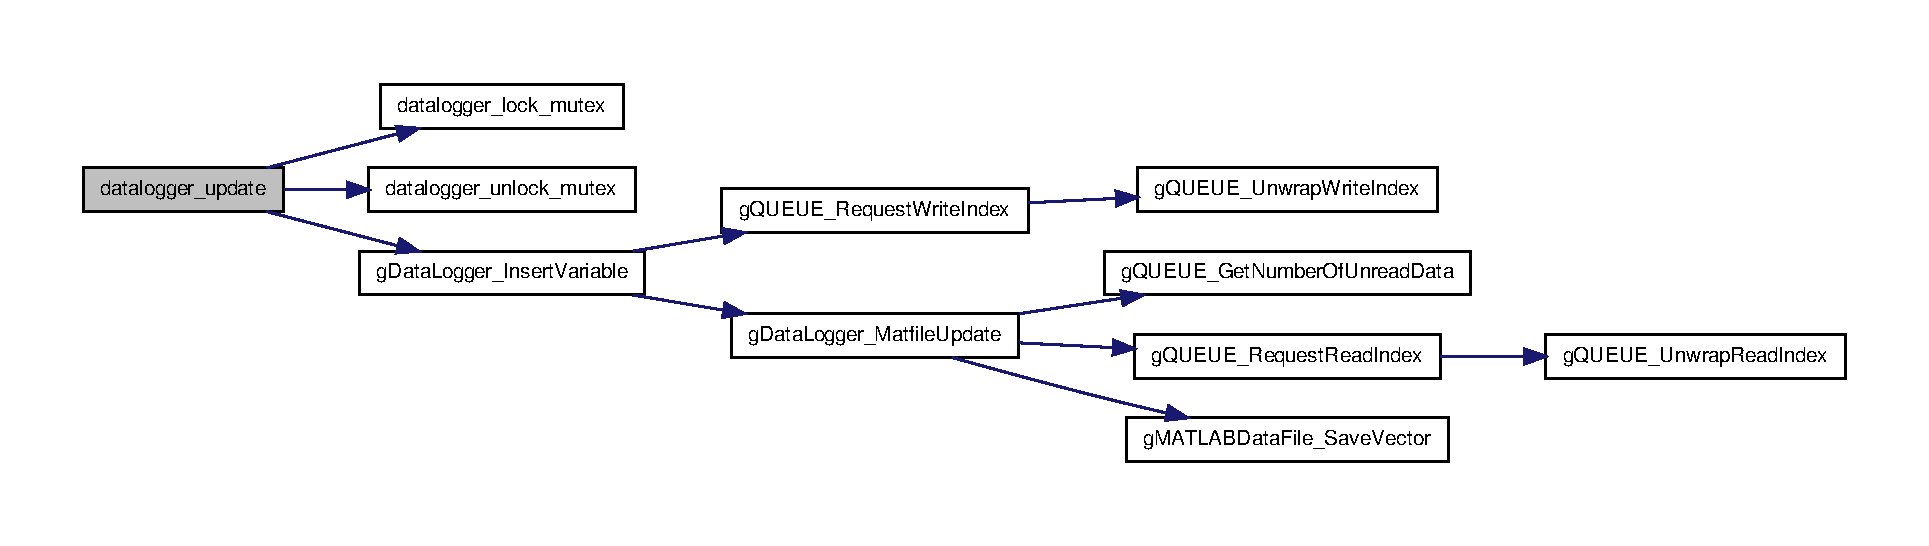
\includegraphics[width=350pt]{datalogger_8c_ad89a56e2f057ace8c28d78eb67703e7d_cgraph}
\end{center}
\end{figure}




Here is the caller graph for this function\-:\nopagebreak
\begin{figure}[H]
\begin{center}
\leavevmode
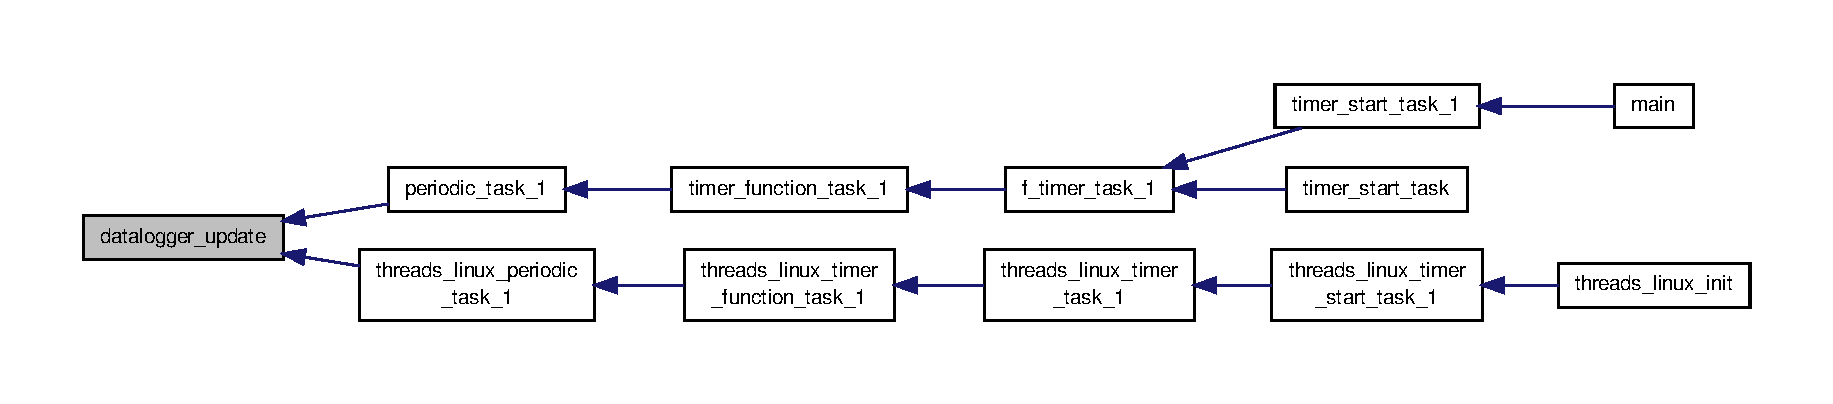
\includegraphics[width=350pt]{datalogger_8c_ad89a56e2f057ace8c28d78eb67703e7d_icgraph}
\end{center}
\end{figure}


\hypertarget{datalogger_8c_a25bb814a0877f419ae09b08cd7e91ee9}{\index{datalogger.\-c@{datalogger.\-c}!datalogger\-\_\-update\-\_\-\-I\-P\-C@{datalogger\-\_\-update\-\_\-\-I\-P\-C}}
\index{datalogger\-\_\-update\-\_\-\-I\-P\-C@{datalogger\-\_\-update\-\_\-\-I\-P\-C}!datalogger.c@{datalogger.\-c}}
\subsubsection[{datalogger\-\_\-update\-\_\-\-I\-P\-C}]{\setlength{\rightskip}{0pt plus 5cm}int datalogger\-\_\-update\-\_\-\-I\-P\-C (
\begin{DoxyParamCaption}
\item[{void}]{}
\end{DoxyParamCaption}
)}}\label{datalogger_8c_a25bb814a0877f419ae09b08cd7e91ee9}


Definition at line 256 of file datalogger.\-c.



References D\-A\-T\-A\-L\-O\-G\-G\-E\-R\-\_\-\-E\-R\-R\-O\-R\-\_\-\-N\-O\-T\-\_\-\-I\-N\-I\-T\-I\-A\-L\-I\-Z\-E\-D, D\-A\-T\-A\-L\-O\-G\-G\-E\-R\-\_\-\-I\-N\-I\-T\-I\-A\-L\-I\-Z\-E\-D, datalogger\-\_\-initialized, datalogger\-\_\-lock\-\_\-mutex(), D\-A\-T\-A\-L\-O\-G\-G\-E\-R\-\_\-\-S\-U\-C\-C\-E\-S\-S, datalogger\-\_\-unlock\-\_\-mutex(), and g\-Data\-Logger\-\_\-\-I\-P\-C\-Update().



Referenced by threads\-\_\-linux\-\_\-init().


\begin{DoxyCode}
\{
\textcolor{preprocessor}{    #if DATALOGGER\_MODULE\_ENABLED}
\textcolor{preprocessor}{}    \hyperlink{datalogger_8c_a54b06d9395b2e370a5a72beb7f9524b2}{datalogger\_lock\_mutex}();
    \textcolor{keywordflow}{if}(\hyperlink{datalogger_8c_a35e8fbe04b90452afdc3c1be16ff6187}{datalogger\_initialized} != \hyperlink{datalogger_8h_a684c343d340004b77ca2b782934c96ca}{DATALOGGER\_INITIALIZED}
      )
    \{
        \hyperlink{datalogger_8c_a85453211c0c809083c36cc56b275aeeb}{datalogger\_unlock\_mutex}();
        \textcolor{keywordflow}{return} \hyperlink{datalogger_8h_a60df7fe0e61b757ad6a9db106b0eb43e}{DATALOGGER\_ERROR\_NOT\_INITIALIZED}
      ;
    \}

    \hyperlink{gdatalogger_8c_afa42a993493cf98d32da11e4279816f7}{gDataLogger\_IPCUpdate}(&\hyperlink{datalogger_8c_abe3b9c2c4e21e79c7b046b5986d13acc}{gDataLogger}); \textcolor{comment}{//
       Manages IPC}
    \hyperlink{datalogger_8c_a85453211c0c809083c36cc56b275aeeb}{datalogger\_unlock\_mutex}();
\textcolor{preprocessor}{    #endif}
\textcolor{preprocessor}{}    \textcolor{keywordflow}{return} \hyperlink{datalogger_8h_abddebaf71d26d40183fccbb1a766b983}{DATALOGGER\_SUCCESS};
\}
\end{DoxyCode}


Here is the call graph for this function\-:\nopagebreak
\begin{figure}[H]
\begin{center}
\leavevmode
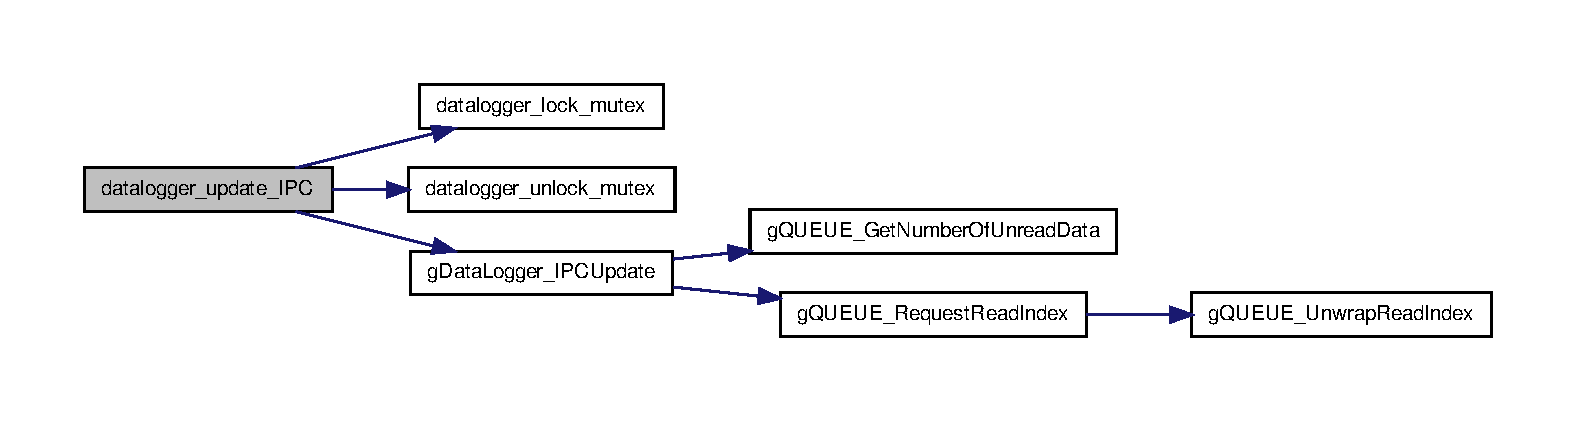
\includegraphics[width=350pt]{datalogger_8c_a25bb814a0877f419ae09b08cd7e91ee9_cgraph}
\end{center}
\end{figure}




Here is the caller graph for this function\-:\nopagebreak
\begin{figure}[H]
\begin{center}
\leavevmode
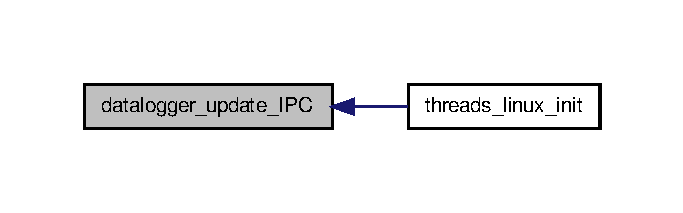
\includegraphics[width=328pt]{datalogger_8c_a25bb814a0877f419ae09b08cd7e91ee9_icgraph}
\end{center}
\end{figure}


\hypertarget{datalogger_8c_a2aedecfce53e1935a41615ceaf378013}{\index{datalogger.\-c@{datalogger.\-c}!datalogger\-\_\-write\-\_\-file@{datalogger\-\_\-write\-\_\-file}}
\index{datalogger\-\_\-write\-\_\-file@{datalogger\-\_\-write\-\_\-file}!datalogger.c@{datalogger.\-c}}
\subsubsection[{datalogger\-\_\-write\-\_\-file}]{\setlength{\rightskip}{0pt plus 5cm}int datalogger\-\_\-write\-\_\-file (
\begin{DoxyParamCaption}
\item[{void}]{}
\end{DoxyParamCaption}
)}}\label{datalogger_8c_a2aedecfce53e1935a41615ceaf378013}


Definition at line 240 of file datalogger.\-c.



References D\-A\-T\-A\-L\-O\-G\-G\-E\-R\-\_\-\-E\-R\-R\-O\-R\-\_\-\-N\-O\-T\-\_\-\-I\-N\-I\-T\-I\-A\-L\-I\-Z\-E\-D, D\-A\-T\-A\-L\-O\-G\-G\-E\-R\-\_\-\-I\-N\-I\-T\-I\-A\-L\-I\-Z\-E\-D, datalogger\-\_\-initialized, datalogger\-\_\-lock\-\_\-mutex(), D\-A\-T\-A\-L\-O\-G\-G\-E\-R\-\_\-\-S\-U\-C\-C\-E\-S\-S, datalogger\-\_\-unlock\-\_\-mutex(), and g\-Data\-Logger\-\_\-\-Matfile\-Update().



Referenced by main(), and threads\-\_\-linux\-\_\-init().


\begin{DoxyCode}
\{
\textcolor{preprocessor}{    #if DATALOGGER\_MODULE\_ENABLED}
\textcolor{preprocessor}{}    \hyperlink{datalogger_8c_a54b06d9395b2e370a5a72beb7f9524b2}{datalogger\_lock\_mutex}();
    \textcolor{keywordflow}{if}(\hyperlink{datalogger_8c_a35e8fbe04b90452afdc3c1be16ff6187}{datalogger\_initialized} != \hyperlink{datalogger_8h_a684c343d340004b77ca2b782934c96ca}{DATALOGGER\_INITIALIZED}
      )
    \{
        \hyperlink{datalogger_8c_a85453211c0c809083c36cc56b275aeeb}{datalogger\_unlock\_mutex}();
        \textcolor{keywordflow}{return} \hyperlink{datalogger_8h_a60df7fe0e61b757ad6a9db106b0eb43e}{DATALOGGER\_ERROR\_NOT\_INITIALIZED}
      ;
    \}
    \hyperlink{gdatalogger_8c_a05dc8ce832b941280d7de26057992640}{gDataLogger\_MatfileUpdate}(&\hyperlink{datalogger_8c_abe3b9c2c4e21e79c7b046b5986d13acc}{gDataLogger})
      ; \textcolor{comment}{// Empty buffers in the file}
    \hyperlink{datalogger_8c_a85453211c0c809083c36cc56b275aeeb}{datalogger\_unlock\_mutex}();
\textcolor{preprocessor}{    #endif}
\textcolor{preprocessor}{}
    \textcolor{keywordflow}{return} \hyperlink{datalogger_8h_abddebaf71d26d40183fccbb1a766b983}{DATALOGGER\_SUCCESS};
\}
\end{DoxyCode}


Here is the call graph for this function\-:\nopagebreak
\begin{figure}[H]
\begin{center}
\leavevmode
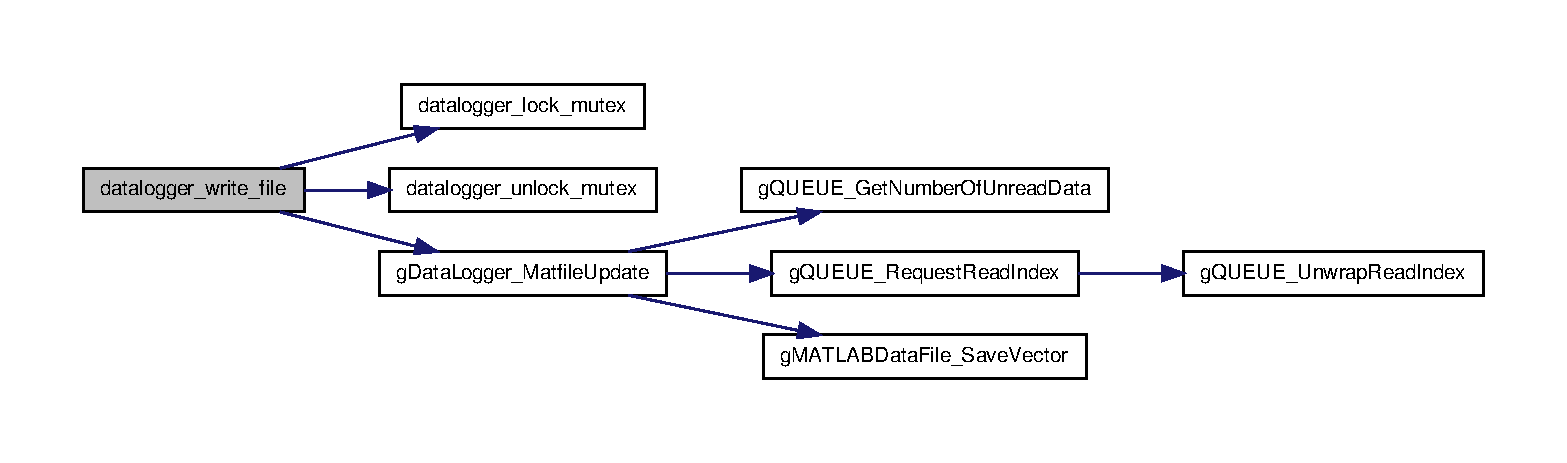
\includegraphics[width=350pt]{datalogger_8c_a2aedecfce53e1935a41615ceaf378013_cgraph}
\end{center}
\end{figure}




Here is the caller graph for this function\-:\nopagebreak
\begin{figure}[H]
\begin{center}
\leavevmode
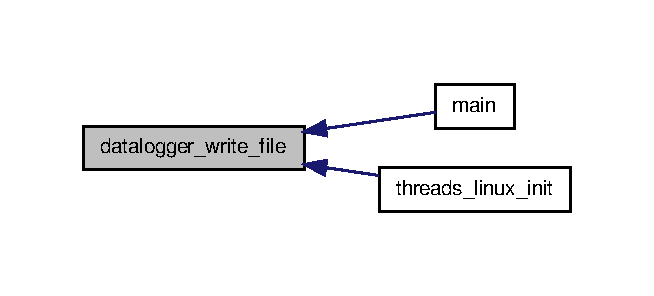
\includegraphics[width=314pt]{datalogger_8c_a2aedecfce53e1935a41615ceaf378013_icgraph}
\end{center}
\end{figure}




\subsection{Variable Documentation}
\hypertarget{datalogger_8c_a35e8fbe04b90452afdc3c1be16ff6187}{\index{datalogger.\-c@{datalogger.\-c}!datalogger\-\_\-initialized@{datalogger\-\_\-initialized}}
\index{datalogger\-\_\-initialized@{datalogger\-\_\-initialized}!datalogger.c@{datalogger.\-c}}
\subsubsection[{datalogger\-\_\-initialized}]{\setlength{\rightskip}{0pt plus 5cm}unsigned int datalogger\-\_\-initialized = {\bf D\-A\-T\-A\-L\-O\-G\-G\-E\-R\-\_\-\-N\-O\-T\-\_\-\-I\-N\-I\-T\-I\-A\-L\-I\-Z\-E\-D}}}\label{datalogger_8c_a35e8fbe04b90452afdc3c1be16ff6187}


Definition at line 29 of file datalogger.\-c.



Referenced by datalogger\-\_\-close(), datalogger\-\_\-init(), datalogger\-\_\-set\-\_\-\-Ts(), datalogger\-\_\-start(), datalogger\-\_\-status(), datalogger\-\_\-stop(), datalogger\-\_\-update(), datalogger\-\_\-update\-\_\-\-I\-P\-C(), and datalogger\-\_\-write\-\_\-file().

\hypertarget{datalogger_8c_a824d6f7fd1d3898ba0b1100ba37875c6}{\index{datalogger.\-c@{datalogger.\-c}!datalogger\-\_\-mutex@{datalogger\-\_\-mutex}}
\index{datalogger\-\_\-mutex@{datalogger\-\_\-mutex}!datalogger.c@{datalogger.\-c}}
\subsubsection[{datalogger\-\_\-mutex}]{\setlength{\rightskip}{0pt plus 5cm}pthread\-\_\-mutex\-\_\-t datalogger\-\_\-mutex = P\-T\-H\-R\-E\-A\-D\-\_\-\-M\-U\-T\-E\-X\-\_\-\-I\-N\-I\-T\-I\-A\-L\-I\-Z\-E\-R}}\label{datalogger_8c_a824d6f7fd1d3898ba0b1100ba37875c6}


Definition at line 34 of file datalogger.\-c.



Referenced by datalogger\-\_\-close(), datalogger\-\_\-init(), datalogger\-\_\-lock\-\_\-mutex(), and datalogger\-\_\-unlock\-\_\-mutex().

\hypertarget{datalogger_8c_a185c3ede96449d14f330fe5ac664e799}{\index{datalogger.\-c@{datalogger.\-c}!datalogger\-\_\-running@{datalogger\-\_\-running}}
\index{datalogger\-\_\-running@{datalogger\-\_\-running}!datalogger.c@{datalogger.\-c}}
\subsubsection[{datalogger\-\_\-running}]{\setlength{\rightskip}{0pt plus 5cm}unsigned int datalogger\-\_\-running = {\bf D\-A\-T\-A\-L\-O\-G\-G\-E\-R\-\_\-\-N\-O\-T\-\_\-\-R\-U\-N\-N\-I\-N\-G}}}\label{datalogger_8c_a185c3ede96449d14f330fe5ac664e799}


Definition at line 30 of file datalogger.\-c.



Referenced by datalogger\-\_\-init(), datalogger\-\_\-start(), datalogger\-\_\-status(), and datalogger\-\_\-stop().

\hypertarget{datalogger_8c_abe3b9c2c4e21e79c7b046b5986d13acc}{\index{datalogger.\-c@{datalogger.\-c}!g\-Data\-Logger@{g\-Data\-Logger}}
\index{g\-Data\-Logger@{g\-Data\-Logger}!datalogger.c@{datalogger.\-c}}
\subsubsection[{g\-Data\-Logger}]{\setlength{\rightskip}{0pt plus 5cm}{\bf G\-D\-A\-T\-A\-L\-O\-G\-G\-E\-R} g\-Data\-Logger}}\label{datalogger_8c_abe3b9c2c4e21e79c7b046b5986d13acc}


Definition at line 28 of file datalogger.\-c.


\hypertarget{datalogger_8h}{\section{datalogger.\-h File Reference}
\label{datalogger_8h}\index{datalogger.\-h@{datalogger.\-h}}
}
This graph shows which files directly or indirectly include this file\-:
\nopagebreak
\begin{figure}[H]
\begin{center}
\leavevmode
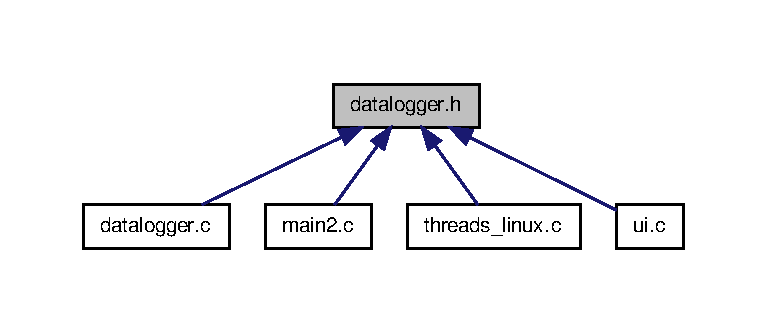
\includegraphics[width=350pt]{datalogger_8h__dep__incl}
\end{center}
\end{figure}
\subsection*{Macros}
\begin{DoxyCompactItemize}
\item 
\#define \hyperlink{datalogger_8h_ac8cb2695f86c0cbaffc8a955d446bcd8}{D\-A\-T\-A\-L\-O\-G\-G\-E\-R\-\_\-\-M\-O\-D\-U\-L\-E\-\_\-\-E\-N\-A\-B\-L\-E\-D}~0
\item 
\#define \hyperlink{datalogger_8h_ae7698fd72f0fc0920eba24d963a25d5a}{D\-A\-T\-A\-L\-O\-G\-G\-E\-R\-\_\-\-D\-E\-B\-U\-G\-\_\-\-M\-O\-D\-E}~0
\item 
\#define \hyperlink{datalogger_8h_a88583f16b8f2052b817854218252cd3e}{D\-A\-T\-A\-L\-O\-G\-G\-E\-R\-\_\-\-E\-N\-A\-B\-L\-E\-\_\-\-N\-E\-W\-\_\-\-F\-I\-L\-E\-\_\-\-E\-N\-N\-U\-M\-E\-R\-A\-T\-I\-O\-N}~1
\item 
\#define \hyperlink{datalogger_8h_a23bf1fb88a2adab92e7c477d927b241c}{D\-A\-T\-A\-L\-O\-G\-G\-E\-R\-\_\-\-F\-I\-L\-E\-\_\-\-N\-A\-M\-E}~\char`\"{}rleg\char`\"{}
\item 
\#define \hyperlink{datalogger_8h_a29791c024463d251eeab6973a0299e7b}{D\-A\-T\-A\-L\-O\-G\-G\-E\-R\-\_\-\-F\-O\-L\-D\-E\-R}~\char`\"{}matlabdatafiles\char`\"{}
\item 
\#define \hyperlink{datalogger_8h_ac244ccff7e47d7f9e79c1b606664f4fa}{D\-A\-T\-A\-L\-O\-G\-G\-E\-R\-\_\-\-S\-T\-A\-N\-D\-A\-R\-D\-\_\-\-Q\-U\-E\-U\-E\-\_\-\-S\-I\-Z\-E}~750
\item 
\#define \hyperlink{datalogger_8h_a9796dd7063d48a850456a4542c5a5fb5}{D\-A\-T\-A\-L\-O\-G\-G\-E\-R\-\_\-\-L\-O\-G\-\_\-\-T\-I\-M\-E}~1
\item 
\#define \hyperlink{datalogger_8h_ade62d89afc68e01d78fa75ae491a9980}{D\-A\-T\-A\-L\-O\-G\-G\-E\-R\-\_\-\-L\-O\-G\-\_\-\-E\-X\-E\-C\-T\-I\-M\-E\-S}~1
\item 
\#define \hyperlink{datalogger_8h_a1c623aa143d8b2e0d507e23425a02275}{D\-A\-T\-A\-L\-O\-G\-G\-E\-R\-\_\-\-L\-O\-G\-\_\-\-R\-A\-W\-\_\-\-I\-M\-U}~1
\item 
\#define \hyperlink{datalogger_8h_a210c5f76b25cb165226a337189a9715f}{D\-A\-T\-A\-L\-O\-G\-G\-E\-R\-\_\-\-L\-O\-G\-\_\-\-E\-F\-F\-O\-R\-T\-S}~1
\item 
\#define \hyperlink{datalogger_8h_ab2e9ad670e20d71c67230b1f064a0dcb}{D\-A\-T\-A\-L\-O\-G\-G\-E\-R\-\_\-\-L\-O\-G\-\_\-\-M\-R\-A}~1
\item 
\#define \hyperlink{datalogger_8h_aa80b147e8c585f7f630658025c24cd8c}{D\-A\-T\-A\-L\-O\-G\-G\-E\-R\-\_\-\-L\-O\-G\-\_\-\-C\-A\-L\-I\-B\-R\-A\-T\-E\-D\-\_\-\-I\-M\-U}~1
\item 
\#define \hyperlink{datalogger_8h_a4602a65fdfa920dfe832cfa50b7ee4c8}{D\-A\-T\-A\-L\-O\-G\-G\-E\-R\-\_\-\-N\-O\-T\-\_\-\-I\-N\-I\-T\-I\-A\-L\-I\-Z\-E\-D}~0
\item 
\#define \hyperlink{datalogger_8h_a684c343d340004b77ca2b782934c96ca}{D\-A\-T\-A\-L\-O\-G\-G\-E\-R\-\_\-\-I\-N\-I\-T\-I\-A\-L\-I\-Z\-E\-D}~1
\item 
\#define \hyperlink{datalogger_8h_a1a224da36800f52f56f30619849f7f5d}{D\-A\-T\-A\-L\-O\-G\-G\-E\-R\-\_\-\-N\-O\-T\-\_\-\-R\-U\-N\-N\-I\-N\-G}~0
\item 
\#define \hyperlink{datalogger_8h_a2cf92051a019c8ec1b5c4f5380758f62}{D\-A\-T\-A\-L\-O\-G\-G\-E\-R\-\_\-\-R\-U\-N\-N\-I\-N\-G}~1
\item 
\#define \hyperlink{datalogger_8h_a1f4fd2dbd981cf35467ab688c9157a74}{D\-A\-T\-A\-L\-O\-G\-G\-E\-R\-\_\-\-V\-A\-R\-I\-A\-B\-L\-E\-\_\-\-N\-O\-T\-\_\-\-I\-N\-S\-E\-R\-T\-E\-D}~0
\item 
\#define \hyperlink{datalogger_8h_a181f9a0649abd26c74ed1a8a1710e25f}{D\-A\-T\-A\-L\-O\-G\-G\-E\-R\-\_\-\-V\-A\-R\-I\-A\-B\-L\-E\-\_\-\-I\-N\-S\-E\-R\-T\-E\-D}~1
\item 
\#define \hyperlink{datalogger_8h_abddebaf71d26d40183fccbb1a766b983}{D\-A\-T\-A\-L\-O\-G\-G\-E\-R\-\_\-\-S\-U\-C\-C\-E\-S\-S}~1
\item 
\#define \hyperlink{datalogger_8h_ac52138ca42979f6e1f1d589020ff9f83}{D\-A\-T\-A\-L\-O\-G\-G\-E\-R\-\_\-\-F\-A\-I\-L\-U\-R\-E}~-\/1
\item 
\#define \hyperlink{datalogger_8h_a60df7fe0e61b757ad6a9db106b0eb43e}{D\-A\-T\-A\-L\-O\-G\-G\-E\-R\-\_\-\-E\-R\-R\-O\-R\-\_\-\-N\-O\-T\-\_\-\-I\-N\-I\-T\-I\-A\-L\-I\-Z\-E\-D}~-\/2
\item 
\#define \hyperlink{datalogger_8h_ac76269a113d60c063e857d14e4a2f640}{D\-A\-T\-A\-L\-O\-G\-G\-E\-R\-\_\-\-V\-A\-R\-I\-B\-A\-L\-E\-\_\-\-A\-L\-R\-E\-A\-D\-Y\-\_\-\-I\-N\-S\-E\-R\-T\-E\-D}~-\/3
\end{DoxyCompactItemize}
\subsection*{Functions}
\begin{DoxyCompactItemize}
\item 
int \hyperlink{datalogger_8h_a1977ef253746fd8c008a3641d9822551}{datalogger\-\_\-init} (void)
\item 
int \hyperlink{datalogger_8h_ad22dbe9e235e7ae5737a23796d13ffbd}{datalogger\-\_\-close} (void)
\item 
int \hyperlink{datalogger_8h_a2aedecfce53e1935a41615ceaf378013}{datalogger\-\_\-write\-\_\-file} (void)
\item 
int \hyperlink{datalogger_8h_a25bb814a0877f419ae09b08cd7e91ee9}{datalogger\-\_\-update\-\_\-\-I\-P\-C} (void)
\item 
int \hyperlink{datalogger_8h_ad89a56e2f057ace8c28d78eb67703e7d}{datalogger\-\_\-update} (double t\-\_\-s, double t\-\_\-control\-\_\-exec\-\_\-s, double t\-\_\-ui\-\_\-exec\-\_\-s, double t0\-\_\-s, \hyperlink{structIMU__DATA__STRUCT}{I\-M\-U\-\_\-\-D\-A\-T\-A\-\_\-\-S\-T\-R\-U\-C\-T} $\ast$pimu\-\_\-data, \hyperlink{structEFF__DATA__STRUCT}{E\-F\-F\-\_\-\-D\-A\-T\-A\-\_\-\-S\-T\-R\-U\-C\-T} $\ast$peff\-\_\-data, \hyperlink{structMRA__DATA__STRUCT}{M\-R\-A\-\_\-\-D\-A\-T\-A\-\_\-\-S\-T\-R\-U\-C\-T} $\ast$pmra\-\_\-data)
\item 
int \hyperlink{datalogger_8h_afb69d166f8d53042825174cee225ea49}{datalogger\-\_\-set\-\_\-\-Ts} (double Ts)
\item 
int \hyperlink{datalogger_8h_a46fd1290d9ee97d5fc7171e1e0dcb0aa}{datalogger\-\_\-status} (void)
\item 
int \hyperlink{datalogger_8h_a1f254ef380d595d6605c10811fd0dee6}{datalogger\-\_\-start} (void)
\item 
int \hyperlink{datalogger_8h_aae2ffbc6cbf8f1cfecceb42c5139530a}{datalogger\-\_\-stop} (void)
\item 
int \hyperlink{datalogger_8h_a29bc3190cba1f225ad3b2eed899a6762}{datalogger\-\_\-file\-\_\-exists} (const char $\ast$filename)
\end{DoxyCompactItemize}


\subsection{Macro Definition Documentation}
\hypertarget{datalogger_8h_ae7698fd72f0fc0920eba24d963a25d5a}{\index{datalogger.\-h@{datalogger.\-h}!D\-A\-T\-A\-L\-O\-G\-G\-E\-R\-\_\-\-D\-E\-B\-U\-G\-\_\-\-M\-O\-D\-E@{D\-A\-T\-A\-L\-O\-G\-G\-E\-R\-\_\-\-D\-E\-B\-U\-G\-\_\-\-M\-O\-D\-E}}
\index{D\-A\-T\-A\-L\-O\-G\-G\-E\-R\-\_\-\-D\-E\-B\-U\-G\-\_\-\-M\-O\-D\-E@{D\-A\-T\-A\-L\-O\-G\-G\-E\-R\-\_\-\-D\-E\-B\-U\-G\-\_\-\-M\-O\-D\-E}!datalogger.h@{datalogger.\-h}}
\subsubsection[{D\-A\-T\-A\-L\-O\-G\-G\-E\-R\-\_\-\-D\-E\-B\-U\-G\-\_\-\-M\-O\-D\-E}]{\setlength{\rightskip}{0pt plus 5cm}\#define D\-A\-T\-A\-L\-O\-G\-G\-E\-R\-\_\-\-D\-E\-B\-U\-G\-\_\-\-M\-O\-D\-E~0}}\label{datalogger_8h_ae7698fd72f0fc0920eba24d963a25d5a}


Definition at line 6 of file datalogger.\-h.

\hypertarget{datalogger_8h_a88583f16b8f2052b817854218252cd3e}{\index{datalogger.\-h@{datalogger.\-h}!D\-A\-T\-A\-L\-O\-G\-G\-E\-R\-\_\-\-E\-N\-A\-B\-L\-E\-\_\-\-N\-E\-W\-\_\-\-F\-I\-L\-E\-\_\-\-E\-N\-N\-U\-M\-E\-R\-A\-T\-I\-O\-N@{D\-A\-T\-A\-L\-O\-G\-G\-E\-R\-\_\-\-E\-N\-A\-B\-L\-E\-\_\-\-N\-E\-W\-\_\-\-F\-I\-L\-E\-\_\-\-E\-N\-N\-U\-M\-E\-R\-A\-T\-I\-O\-N}}
\index{D\-A\-T\-A\-L\-O\-G\-G\-E\-R\-\_\-\-E\-N\-A\-B\-L\-E\-\_\-\-N\-E\-W\-\_\-\-F\-I\-L\-E\-\_\-\-E\-N\-N\-U\-M\-E\-R\-A\-T\-I\-O\-N@{D\-A\-T\-A\-L\-O\-G\-G\-E\-R\-\_\-\-E\-N\-A\-B\-L\-E\-\_\-\-N\-E\-W\-\_\-\-F\-I\-L\-E\-\_\-\-E\-N\-N\-U\-M\-E\-R\-A\-T\-I\-O\-N}!datalogger.h@{datalogger.\-h}}
\subsubsection[{D\-A\-T\-A\-L\-O\-G\-G\-E\-R\-\_\-\-E\-N\-A\-B\-L\-E\-\_\-\-N\-E\-W\-\_\-\-F\-I\-L\-E\-\_\-\-E\-N\-N\-U\-M\-E\-R\-A\-T\-I\-O\-N}]{\setlength{\rightskip}{0pt plus 5cm}\#define D\-A\-T\-A\-L\-O\-G\-G\-E\-R\-\_\-\-E\-N\-A\-B\-L\-E\-\_\-\-N\-E\-W\-\_\-\-F\-I\-L\-E\-\_\-\-E\-N\-N\-U\-M\-E\-R\-A\-T\-I\-O\-N~1}}\label{datalogger_8h_a88583f16b8f2052b817854218252cd3e}


Definition at line 9 of file datalogger.\-h.

\hypertarget{datalogger_8h_a60df7fe0e61b757ad6a9db106b0eb43e}{\index{datalogger.\-h@{datalogger.\-h}!D\-A\-T\-A\-L\-O\-G\-G\-E\-R\-\_\-\-E\-R\-R\-O\-R\-\_\-\-N\-O\-T\-\_\-\-I\-N\-I\-T\-I\-A\-L\-I\-Z\-E\-D@{D\-A\-T\-A\-L\-O\-G\-G\-E\-R\-\_\-\-E\-R\-R\-O\-R\-\_\-\-N\-O\-T\-\_\-\-I\-N\-I\-T\-I\-A\-L\-I\-Z\-E\-D}}
\index{D\-A\-T\-A\-L\-O\-G\-G\-E\-R\-\_\-\-E\-R\-R\-O\-R\-\_\-\-N\-O\-T\-\_\-\-I\-N\-I\-T\-I\-A\-L\-I\-Z\-E\-D@{D\-A\-T\-A\-L\-O\-G\-G\-E\-R\-\_\-\-E\-R\-R\-O\-R\-\_\-\-N\-O\-T\-\_\-\-I\-N\-I\-T\-I\-A\-L\-I\-Z\-E\-D}!datalogger.h@{datalogger.\-h}}
\subsubsection[{D\-A\-T\-A\-L\-O\-G\-G\-E\-R\-\_\-\-E\-R\-R\-O\-R\-\_\-\-N\-O\-T\-\_\-\-I\-N\-I\-T\-I\-A\-L\-I\-Z\-E\-D}]{\setlength{\rightskip}{0pt plus 5cm}\#define D\-A\-T\-A\-L\-O\-G\-G\-E\-R\-\_\-\-E\-R\-R\-O\-R\-\_\-\-N\-O\-T\-\_\-\-I\-N\-I\-T\-I\-A\-L\-I\-Z\-E\-D~-\/2}}\label{datalogger_8h_a60df7fe0e61b757ad6a9db106b0eb43e}


Definition at line 37 of file datalogger.\-h.



Referenced by datalogger\-\_\-close(), datalogger\-\_\-set\-\_\-\-Ts(), datalogger\-\_\-start(), datalogger\-\_\-status(), datalogger\-\_\-stop(), datalogger\-\_\-update(), datalogger\-\_\-update\-\_\-\-I\-P\-C(), and datalogger\-\_\-write\-\_\-file().

\hypertarget{datalogger_8h_ac52138ca42979f6e1f1d589020ff9f83}{\index{datalogger.\-h@{datalogger.\-h}!D\-A\-T\-A\-L\-O\-G\-G\-E\-R\-\_\-\-F\-A\-I\-L\-U\-R\-E@{D\-A\-T\-A\-L\-O\-G\-G\-E\-R\-\_\-\-F\-A\-I\-L\-U\-R\-E}}
\index{D\-A\-T\-A\-L\-O\-G\-G\-E\-R\-\_\-\-F\-A\-I\-L\-U\-R\-E@{D\-A\-T\-A\-L\-O\-G\-G\-E\-R\-\_\-\-F\-A\-I\-L\-U\-R\-E}!datalogger.h@{datalogger.\-h}}
\subsubsection[{D\-A\-T\-A\-L\-O\-G\-G\-E\-R\-\_\-\-F\-A\-I\-L\-U\-R\-E}]{\setlength{\rightskip}{0pt plus 5cm}\#define D\-A\-T\-A\-L\-O\-G\-G\-E\-R\-\_\-\-F\-A\-I\-L\-U\-R\-E~-\/1}}\label{datalogger_8h_ac52138ca42979f6e1f1d589020ff9f83}


Definition at line 36 of file datalogger.\-h.



Referenced by datalogger\-\_\-file\-\_\-exists(), and datalogger\-\_\-init().

\hypertarget{datalogger_8h_a23bf1fb88a2adab92e7c477d927b241c}{\index{datalogger.\-h@{datalogger.\-h}!D\-A\-T\-A\-L\-O\-G\-G\-E\-R\-\_\-\-F\-I\-L\-E\-\_\-\-N\-A\-M\-E@{D\-A\-T\-A\-L\-O\-G\-G\-E\-R\-\_\-\-F\-I\-L\-E\-\_\-\-N\-A\-M\-E}}
\index{D\-A\-T\-A\-L\-O\-G\-G\-E\-R\-\_\-\-F\-I\-L\-E\-\_\-\-N\-A\-M\-E@{D\-A\-T\-A\-L\-O\-G\-G\-E\-R\-\_\-\-F\-I\-L\-E\-\_\-\-N\-A\-M\-E}!datalogger.h@{datalogger.\-h}}
\subsubsection[{D\-A\-T\-A\-L\-O\-G\-G\-E\-R\-\_\-\-F\-I\-L\-E\-\_\-\-N\-A\-M\-E}]{\setlength{\rightskip}{0pt plus 5cm}\#define D\-A\-T\-A\-L\-O\-G\-G\-E\-R\-\_\-\-F\-I\-L\-E\-\_\-\-N\-A\-M\-E~\char`\"{}rleg\char`\"{}}}\label{datalogger_8h_a23bf1fb88a2adab92e7c477d927b241c}


Definition at line 10 of file datalogger.\-h.



Referenced by datalogger\-\_\-init().

\hypertarget{datalogger_8h_a29791c024463d251eeab6973a0299e7b}{\index{datalogger.\-h@{datalogger.\-h}!D\-A\-T\-A\-L\-O\-G\-G\-E\-R\-\_\-\-F\-O\-L\-D\-E\-R@{D\-A\-T\-A\-L\-O\-G\-G\-E\-R\-\_\-\-F\-O\-L\-D\-E\-R}}
\index{D\-A\-T\-A\-L\-O\-G\-G\-E\-R\-\_\-\-F\-O\-L\-D\-E\-R@{D\-A\-T\-A\-L\-O\-G\-G\-E\-R\-\_\-\-F\-O\-L\-D\-E\-R}!datalogger.h@{datalogger.\-h}}
\subsubsection[{D\-A\-T\-A\-L\-O\-G\-G\-E\-R\-\_\-\-F\-O\-L\-D\-E\-R}]{\setlength{\rightskip}{0pt plus 5cm}\#define D\-A\-T\-A\-L\-O\-G\-G\-E\-R\-\_\-\-F\-O\-L\-D\-E\-R~\char`\"{}matlabdatafiles\char`\"{}}}\label{datalogger_8h_a29791c024463d251eeab6973a0299e7b}


Definition at line 11 of file datalogger.\-h.



Referenced by datalogger\-\_\-init().

\hypertarget{datalogger_8h_a684c343d340004b77ca2b782934c96ca}{\index{datalogger.\-h@{datalogger.\-h}!D\-A\-T\-A\-L\-O\-G\-G\-E\-R\-\_\-\-I\-N\-I\-T\-I\-A\-L\-I\-Z\-E\-D@{D\-A\-T\-A\-L\-O\-G\-G\-E\-R\-\_\-\-I\-N\-I\-T\-I\-A\-L\-I\-Z\-E\-D}}
\index{D\-A\-T\-A\-L\-O\-G\-G\-E\-R\-\_\-\-I\-N\-I\-T\-I\-A\-L\-I\-Z\-E\-D@{D\-A\-T\-A\-L\-O\-G\-G\-E\-R\-\_\-\-I\-N\-I\-T\-I\-A\-L\-I\-Z\-E\-D}!datalogger.h@{datalogger.\-h}}
\subsubsection[{D\-A\-T\-A\-L\-O\-G\-G\-E\-R\-\_\-\-I\-N\-I\-T\-I\-A\-L\-I\-Z\-E\-D}]{\setlength{\rightskip}{0pt plus 5cm}\#define D\-A\-T\-A\-L\-O\-G\-G\-E\-R\-\_\-\-I\-N\-I\-T\-I\-A\-L\-I\-Z\-E\-D~1}}\label{datalogger_8h_a684c343d340004b77ca2b782934c96ca}


Definition at line 28 of file datalogger.\-h.



Referenced by datalogger\-\_\-close(), datalogger\-\_\-init(), datalogger\-\_\-set\-\_\-\-Ts(), datalogger\-\_\-start(), datalogger\-\_\-status(), datalogger\-\_\-stop(), datalogger\-\_\-update(), datalogger\-\_\-update\-\_\-\-I\-P\-C(), and datalogger\-\_\-write\-\_\-file().

\hypertarget{datalogger_8h_aa80b147e8c585f7f630658025c24cd8c}{\index{datalogger.\-h@{datalogger.\-h}!D\-A\-T\-A\-L\-O\-G\-G\-E\-R\-\_\-\-L\-O\-G\-\_\-\-C\-A\-L\-I\-B\-R\-A\-T\-E\-D\-\_\-\-I\-M\-U@{D\-A\-T\-A\-L\-O\-G\-G\-E\-R\-\_\-\-L\-O\-G\-\_\-\-C\-A\-L\-I\-B\-R\-A\-T\-E\-D\-\_\-\-I\-M\-U}}
\index{D\-A\-T\-A\-L\-O\-G\-G\-E\-R\-\_\-\-L\-O\-G\-\_\-\-C\-A\-L\-I\-B\-R\-A\-T\-E\-D\-\_\-\-I\-M\-U@{D\-A\-T\-A\-L\-O\-G\-G\-E\-R\-\_\-\-L\-O\-G\-\_\-\-C\-A\-L\-I\-B\-R\-A\-T\-E\-D\-\_\-\-I\-M\-U}!datalogger.h@{datalogger.\-h}}
\subsubsection[{D\-A\-T\-A\-L\-O\-G\-G\-E\-R\-\_\-\-L\-O\-G\-\_\-\-C\-A\-L\-I\-B\-R\-A\-T\-E\-D\-\_\-\-I\-M\-U}]{\setlength{\rightskip}{0pt plus 5cm}\#define D\-A\-T\-A\-L\-O\-G\-G\-E\-R\-\_\-\-L\-O\-G\-\_\-\-C\-A\-L\-I\-B\-R\-A\-T\-E\-D\-\_\-\-I\-M\-U~1}}\label{datalogger_8h_aa80b147e8c585f7f630658025c24cd8c}


Definition at line 22 of file datalogger.\-h.



Referenced by datalogger\-\_\-init().

\hypertarget{datalogger_8h_a210c5f76b25cb165226a337189a9715f}{\index{datalogger.\-h@{datalogger.\-h}!D\-A\-T\-A\-L\-O\-G\-G\-E\-R\-\_\-\-L\-O\-G\-\_\-\-E\-F\-F\-O\-R\-T\-S@{D\-A\-T\-A\-L\-O\-G\-G\-E\-R\-\_\-\-L\-O\-G\-\_\-\-E\-F\-F\-O\-R\-T\-S}}
\index{D\-A\-T\-A\-L\-O\-G\-G\-E\-R\-\_\-\-L\-O\-G\-\_\-\-E\-F\-F\-O\-R\-T\-S@{D\-A\-T\-A\-L\-O\-G\-G\-E\-R\-\_\-\-L\-O\-G\-\_\-\-E\-F\-F\-O\-R\-T\-S}!datalogger.h@{datalogger.\-h}}
\subsubsection[{D\-A\-T\-A\-L\-O\-G\-G\-E\-R\-\_\-\-L\-O\-G\-\_\-\-E\-F\-F\-O\-R\-T\-S}]{\setlength{\rightskip}{0pt plus 5cm}\#define D\-A\-T\-A\-L\-O\-G\-G\-E\-R\-\_\-\-L\-O\-G\-\_\-\-E\-F\-F\-O\-R\-T\-S~1}}\label{datalogger_8h_a210c5f76b25cb165226a337189a9715f}


Definition at line 18 of file datalogger.\-h.



Referenced by datalogger\-\_\-init().

\hypertarget{datalogger_8h_ade62d89afc68e01d78fa75ae491a9980}{\index{datalogger.\-h@{datalogger.\-h}!D\-A\-T\-A\-L\-O\-G\-G\-E\-R\-\_\-\-L\-O\-G\-\_\-\-E\-X\-E\-C\-T\-I\-M\-E\-S@{D\-A\-T\-A\-L\-O\-G\-G\-E\-R\-\_\-\-L\-O\-G\-\_\-\-E\-X\-E\-C\-T\-I\-M\-E\-S}}
\index{D\-A\-T\-A\-L\-O\-G\-G\-E\-R\-\_\-\-L\-O\-G\-\_\-\-E\-X\-E\-C\-T\-I\-M\-E\-S@{D\-A\-T\-A\-L\-O\-G\-G\-E\-R\-\_\-\-L\-O\-G\-\_\-\-E\-X\-E\-C\-T\-I\-M\-E\-S}!datalogger.h@{datalogger.\-h}}
\subsubsection[{D\-A\-T\-A\-L\-O\-G\-G\-E\-R\-\_\-\-L\-O\-G\-\_\-\-E\-X\-E\-C\-T\-I\-M\-E\-S}]{\setlength{\rightskip}{0pt plus 5cm}\#define D\-A\-T\-A\-L\-O\-G\-G\-E\-R\-\_\-\-L\-O\-G\-\_\-\-E\-X\-E\-C\-T\-I\-M\-E\-S~1}}\label{datalogger_8h_ade62d89afc68e01d78fa75ae491a9980}


Definition at line 16 of file datalogger.\-h.



Referenced by datalogger\-\_\-init().

\hypertarget{datalogger_8h_ab2e9ad670e20d71c67230b1f064a0dcb}{\index{datalogger.\-h@{datalogger.\-h}!D\-A\-T\-A\-L\-O\-G\-G\-E\-R\-\_\-\-L\-O\-G\-\_\-\-M\-R\-A@{D\-A\-T\-A\-L\-O\-G\-G\-E\-R\-\_\-\-L\-O\-G\-\_\-\-M\-R\-A}}
\index{D\-A\-T\-A\-L\-O\-G\-G\-E\-R\-\_\-\-L\-O\-G\-\_\-\-M\-R\-A@{D\-A\-T\-A\-L\-O\-G\-G\-E\-R\-\_\-\-L\-O\-G\-\_\-\-M\-R\-A}!datalogger.h@{datalogger.\-h}}
\subsubsection[{D\-A\-T\-A\-L\-O\-G\-G\-E\-R\-\_\-\-L\-O\-G\-\_\-\-M\-R\-A}]{\setlength{\rightskip}{0pt plus 5cm}\#define D\-A\-T\-A\-L\-O\-G\-G\-E\-R\-\_\-\-L\-O\-G\-\_\-\-M\-R\-A~1}}\label{datalogger_8h_ab2e9ad670e20d71c67230b1f064a0dcb}


Definition at line 19 of file datalogger.\-h.



Referenced by datalogger\-\_\-init().

\hypertarget{datalogger_8h_a1c623aa143d8b2e0d507e23425a02275}{\index{datalogger.\-h@{datalogger.\-h}!D\-A\-T\-A\-L\-O\-G\-G\-E\-R\-\_\-\-L\-O\-G\-\_\-\-R\-A\-W\-\_\-\-I\-M\-U@{D\-A\-T\-A\-L\-O\-G\-G\-E\-R\-\_\-\-L\-O\-G\-\_\-\-R\-A\-W\-\_\-\-I\-M\-U}}
\index{D\-A\-T\-A\-L\-O\-G\-G\-E\-R\-\_\-\-L\-O\-G\-\_\-\-R\-A\-W\-\_\-\-I\-M\-U@{D\-A\-T\-A\-L\-O\-G\-G\-E\-R\-\_\-\-L\-O\-G\-\_\-\-R\-A\-W\-\_\-\-I\-M\-U}!datalogger.h@{datalogger.\-h}}
\subsubsection[{D\-A\-T\-A\-L\-O\-G\-G\-E\-R\-\_\-\-L\-O\-G\-\_\-\-R\-A\-W\-\_\-\-I\-M\-U}]{\setlength{\rightskip}{0pt plus 5cm}\#define D\-A\-T\-A\-L\-O\-G\-G\-E\-R\-\_\-\-L\-O\-G\-\_\-\-R\-A\-W\-\_\-\-I\-M\-U~1}}\label{datalogger_8h_a1c623aa143d8b2e0d507e23425a02275}


Definition at line 17 of file datalogger.\-h.



Referenced by datalogger\-\_\-init().

\hypertarget{datalogger_8h_a9796dd7063d48a850456a4542c5a5fb5}{\index{datalogger.\-h@{datalogger.\-h}!D\-A\-T\-A\-L\-O\-G\-G\-E\-R\-\_\-\-L\-O\-G\-\_\-\-T\-I\-M\-E@{D\-A\-T\-A\-L\-O\-G\-G\-E\-R\-\_\-\-L\-O\-G\-\_\-\-T\-I\-M\-E}}
\index{D\-A\-T\-A\-L\-O\-G\-G\-E\-R\-\_\-\-L\-O\-G\-\_\-\-T\-I\-M\-E@{D\-A\-T\-A\-L\-O\-G\-G\-E\-R\-\_\-\-L\-O\-G\-\_\-\-T\-I\-M\-E}!datalogger.h@{datalogger.\-h}}
\subsubsection[{D\-A\-T\-A\-L\-O\-G\-G\-E\-R\-\_\-\-L\-O\-G\-\_\-\-T\-I\-M\-E}]{\setlength{\rightskip}{0pt plus 5cm}\#define D\-A\-T\-A\-L\-O\-G\-G\-E\-R\-\_\-\-L\-O\-G\-\_\-\-T\-I\-M\-E~1}}\label{datalogger_8h_a9796dd7063d48a850456a4542c5a5fb5}


Definition at line 15 of file datalogger.\-h.



Referenced by datalogger\-\_\-init().

\hypertarget{datalogger_8h_ac8cb2695f86c0cbaffc8a955d446bcd8}{\index{datalogger.\-h@{datalogger.\-h}!D\-A\-T\-A\-L\-O\-G\-G\-E\-R\-\_\-\-M\-O\-D\-U\-L\-E\-\_\-\-E\-N\-A\-B\-L\-E\-D@{D\-A\-T\-A\-L\-O\-G\-G\-E\-R\-\_\-\-M\-O\-D\-U\-L\-E\-\_\-\-E\-N\-A\-B\-L\-E\-D}}
\index{D\-A\-T\-A\-L\-O\-G\-G\-E\-R\-\_\-\-M\-O\-D\-U\-L\-E\-\_\-\-E\-N\-A\-B\-L\-E\-D@{D\-A\-T\-A\-L\-O\-G\-G\-E\-R\-\_\-\-M\-O\-D\-U\-L\-E\-\_\-\-E\-N\-A\-B\-L\-E\-D}!datalogger.h@{datalogger.\-h}}
\subsubsection[{D\-A\-T\-A\-L\-O\-G\-G\-E\-R\-\_\-\-M\-O\-D\-U\-L\-E\-\_\-\-E\-N\-A\-B\-L\-E\-D}]{\setlength{\rightskip}{0pt plus 5cm}\#define D\-A\-T\-A\-L\-O\-G\-G\-E\-R\-\_\-\-M\-O\-D\-U\-L\-E\-\_\-\-E\-N\-A\-B\-L\-E\-D~0}}\label{datalogger_8h_ac8cb2695f86c0cbaffc8a955d446bcd8}


Definition at line 5 of file datalogger.\-h.

\hypertarget{datalogger_8h_a4602a65fdfa920dfe832cfa50b7ee4c8}{\index{datalogger.\-h@{datalogger.\-h}!D\-A\-T\-A\-L\-O\-G\-G\-E\-R\-\_\-\-N\-O\-T\-\_\-\-I\-N\-I\-T\-I\-A\-L\-I\-Z\-E\-D@{D\-A\-T\-A\-L\-O\-G\-G\-E\-R\-\_\-\-N\-O\-T\-\_\-\-I\-N\-I\-T\-I\-A\-L\-I\-Z\-E\-D}}
\index{D\-A\-T\-A\-L\-O\-G\-G\-E\-R\-\_\-\-N\-O\-T\-\_\-\-I\-N\-I\-T\-I\-A\-L\-I\-Z\-E\-D@{D\-A\-T\-A\-L\-O\-G\-G\-E\-R\-\_\-\-N\-O\-T\-\_\-\-I\-N\-I\-T\-I\-A\-L\-I\-Z\-E\-D}!datalogger.h@{datalogger.\-h}}
\subsubsection[{D\-A\-T\-A\-L\-O\-G\-G\-E\-R\-\_\-\-N\-O\-T\-\_\-\-I\-N\-I\-T\-I\-A\-L\-I\-Z\-E\-D}]{\setlength{\rightskip}{0pt plus 5cm}\#define D\-A\-T\-A\-L\-O\-G\-G\-E\-R\-\_\-\-N\-O\-T\-\_\-\-I\-N\-I\-T\-I\-A\-L\-I\-Z\-E\-D~0}}\label{datalogger_8h_a4602a65fdfa920dfe832cfa50b7ee4c8}


Definition at line 27 of file datalogger.\-h.



Referenced by datalogger\-\_\-close().

\hypertarget{datalogger_8h_a1a224da36800f52f56f30619849f7f5d}{\index{datalogger.\-h@{datalogger.\-h}!D\-A\-T\-A\-L\-O\-G\-G\-E\-R\-\_\-\-N\-O\-T\-\_\-\-R\-U\-N\-N\-I\-N\-G@{D\-A\-T\-A\-L\-O\-G\-G\-E\-R\-\_\-\-N\-O\-T\-\_\-\-R\-U\-N\-N\-I\-N\-G}}
\index{D\-A\-T\-A\-L\-O\-G\-G\-E\-R\-\_\-\-N\-O\-T\-\_\-\-R\-U\-N\-N\-I\-N\-G@{D\-A\-T\-A\-L\-O\-G\-G\-E\-R\-\_\-\-N\-O\-T\-\_\-\-R\-U\-N\-N\-I\-N\-G}!datalogger.h@{datalogger.\-h}}
\subsubsection[{D\-A\-T\-A\-L\-O\-G\-G\-E\-R\-\_\-\-N\-O\-T\-\_\-\-R\-U\-N\-N\-I\-N\-G}]{\setlength{\rightskip}{0pt plus 5cm}\#define D\-A\-T\-A\-L\-O\-G\-G\-E\-R\-\_\-\-N\-O\-T\-\_\-\-R\-U\-N\-N\-I\-N\-G~0}}\label{datalogger_8h_a1a224da36800f52f56f30619849f7f5d}


Definition at line 29 of file datalogger.\-h.



Referenced by datalogger\-\_\-init(), datalogger\-\_\-stop(), periodic\-\_\-task\-\_\-1(), and threads\-\_\-linux\-\_\-periodic\-\_\-task\-\_\-1().

\hypertarget{datalogger_8h_a2cf92051a019c8ec1b5c4f5380758f62}{\index{datalogger.\-h@{datalogger.\-h}!D\-A\-T\-A\-L\-O\-G\-G\-E\-R\-\_\-\-R\-U\-N\-N\-I\-N\-G@{D\-A\-T\-A\-L\-O\-G\-G\-E\-R\-\_\-\-R\-U\-N\-N\-I\-N\-G}}
\index{D\-A\-T\-A\-L\-O\-G\-G\-E\-R\-\_\-\-R\-U\-N\-N\-I\-N\-G@{D\-A\-T\-A\-L\-O\-G\-G\-E\-R\-\_\-\-R\-U\-N\-N\-I\-N\-G}!datalogger.h@{datalogger.\-h}}
\subsubsection[{D\-A\-T\-A\-L\-O\-G\-G\-E\-R\-\_\-\-R\-U\-N\-N\-I\-N\-G}]{\setlength{\rightskip}{0pt plus 5cm}\#define D\-A\-T\-A\-L\-O\-G\-G\-E\-R\-\_\-\-R\-U\-N\-N\-I\-N\-G~1}}\label{datalogger_8h_a2cf92051a019c8ec1b5c4f5380758f62}


Definition at line 30 of file datalogger.\-h.



Referenced by datalogger\-\_\-start(), main(), periodic\-\_\-task\-\_\-1(), threads\-\_\-linux\-\_\-init(), and threads\-\_\-linux\-\_\-periodic\-\_\-task\-\_\-1().

\hypertarget{datalogger_8h_ac244ccff7e47d7f9e79c1b606664f4fa}{\index{datalogger.\-h@{datalogger.\-h}!D\-A\-T\-A\-L\-O\-G\-G\-E\-R\-\_\-\-S\-T\-A\-N\-D\-A\-R\-D\-\_\-\-Q\-U\-E\-U\-E\-\_\-\-S\-I\-Z\-E@{D\-A\-T\-A\-L\-O\-G\-G\-E\-R\-\_\-\-S\-T\-A\-N\-D\-A\-R\-D\-\_\-\-Q\-U\-E\-U\-E\-\_\-\-S\-I\-Z\-E}}
\index{D\-A\-T\-A\-L\-O\-G\-G\-E\-R\-\_\-\-S\-T\-A\-N\-D\-A\-R\-D\-\_\-\-Q\-U\-E\-U\-E\-\_\-\-S\-I\-Z\-E@{D\-A\-T\-A\-L\-O\-G\-G\-E\-R\-\_\-\-S\-T\-A\-N\-D\-A\-R\-D\-\_\-\-Q\-U\-E\-U\-E\-\_\-\-S\-I\-Z\-E}!datalogger.h@{datalogger.\-h}}
\subsubsection[{D\-A\-T\-A\-L\-O\-G\-G\-E\-R\-\_\-\-S\-T\-A\-N\-D\-A\-R\-D\-\_\-\-Q\-U\-E\-U\-E\-\_\-\-S\-I\-Z\-E}]{\setlength{\rightskip}{0pt plus 5cm}\#define D\-A\-T\-A\-L\-O\-G\-G\-E\-R\-\_\-\-S\-T\-A\-N\-D\-A\-R\-D\-\_\-\-Q\-U\-E\-U\-E\-\_\-\-S\-I\-Z\-E~750}}\label{datalogger_8h_ac244ccff7e47d7f9e79c1b606664f4fa}


Definition at line 12 of file datalogger.\-h.



Referenced by datalogger\-\_\-init().

\hypertarget{datalogger_8h_abddebaf71d26d40183fccbb1a766b983}{\index{datalogger.\-h@{datalogger.\-h}!D\-A\-T\-A\-L\-O\-G\-G\-E\-R\-\_\-\-S\-U\-C\-C\-E\-S\-S@{D\-A\-T\-A\-L\-O\-G\-G\-E\-R\-\_\-\-S\-U\-C\-C\-E\-S\-S}}
\index{D\-A\-T\-A\-L\-O\-G\-G\-E\-R\-\_\-\-S\-U\-C\-C\-E\-S\-S@{D\-A\-T\-A\-L\-O\-G\-G\-E\-R\-\_\-\-S\-U\-C\-C\-E\-S\-S}!datalogger.h@{datalogger.\-h}}
\subsubsection[{D\-A\-T\-A\-L\-O\-G\-G\-E\-R\-\_\-\-S\-U\-C\-C\-E\-S\-S}]{\setlength{\rightskip}{0pt plus 5cm}\#define D\-A\-T\-A\-L\-O\-G\-G\-E\-R\-\_\-\-S\-U\-C\-C\-E\-S\-S~1}}\label{datalogger_8h_abddebaf71d26d40183fccbb1a766b983}


Definition at line 35 of file datalogger.\-h.



Referenced by datalogger\-\_\-close(), datalogger\-\_\-file\-\_\-exists(), datalogger\-\_\-init(), datalogger\-\_\-lock\-\_\-mutex(), datalogger\-\_\-set\-\_\-\-Ts(), datalogger\-\_\-start(), datalogger\-\_\-stop(), datalogger\-\_\-unlock\-\_\-mutex(), datalogger\-\_\-update(), datalogger\-\_\-update\-\_\-\-I\-P\-C(), datalogger\-\_\-write\-\_\-file(), main(), and threads\-\_\-linux\-\_\-init().

\hypertarget{datalogger_8h_a181f9a0649abd26c74ed1a8a1710e25f}{\index{datalogger.\-h@{datalogger.\-h}!D\-A\-T\-A\-L\-O\-G\-G\-E\-R\-\_\-\-V\-A\-R\-I\-A\-B\-L\-E\-\_\-\-I\-N\-S\-E\-R\-T\-E\-D@{D\-A\-T\-A\-L\-O\-G\-G\-E\-R\-\_\-\-V\-A\-R\-I\-A\-B\-L\-E\-\_\-\-I\-N\-S\-E\-R\-T\-E\-D}}
\index{D\-A\-T\-A\-L\-O\-G\-G\-E\-R\-\_\-\-V\-A\-R\-I\-A\-B\-L\-E\-\_\-\-I\-N\-S\-E\-R\-T\-E\-D@{D\-A\-T\-A\-L\-O\-G\-G\-E\-R\-\_\-\-V\-A\-R\-I\-A\-B\-L\-E\-\_\-\-I\-N\-S\-E\-R\-T\-E\-D}!datalogger.h@{datalogger.\-h}}
\subsubsection[{D\-A\-T\-A\-L\-O\-G\-G\-E\-R\-\_\-\-V\-A\-R\-I\-A\-B\-L\-E\-\_\-\-I\-N\-S\-E\-R\-T\-E\-D}]{\setlength{\rightskip}{0pt plus 5cm}\#define D\-A\-T\-A\-L\-O\-G\-G\-E\-R\-\_\-\-V\-A\-R\-I\-A\-B\-L\-E\-\_\-\-I\-N\-S\-E\-R\-T\-E\-D~1}}\label{datalogger_8h_a181f9a0649abd26c74ed1a8a1710e25f}


Definition at line 32 of file datalogger.\-h.



Referenced by datalogger\-\_\-set\-\_\-\-Ts().

\hypertarget{datalogger_8h_a1f4fd2dbd981cf35467ab688c9157a74}{\index{datalogger.\-h@{datalogger.\-h}!D\-A\-T\-A\-L\-O\-G\-G\-E\-R\-\_\-\-V\-A\-R\-I\-A\-B\-L\-E\-\_\-\-N\-O\-T\-\_\-\-I\-N\-S\-E\-R\-T\-E\-D@{D\-A\-T\-A\-L\-O\-G\-G\-E\-R\-\_\-\-V\-A\-R\-I\-A\-B\-L\-E\-\_\-\-N\-O\-T\-\_\-\-I\-N\-S\-E\-R\-T\-E\-D}}
\index{D\-A\-T\-A\-L\-O\-G\-G\-E\-R\-\_\-\-V\-A\-R\-I\-A\-B\-L\-E\-\_\-\-N\-O\-T\-\_\-\-I\-N\-S\-E\-R\-T\-E\-D@{D\-A\-T\-A\-L\-O\-G\-G\-E\-R\-\_\-\-V\-A\-R\-I\-A\-B\-L\-E\-\_\-\-N\-O\-T\-\_\-\-I\-N\-S\-E\-R\-T\-E\-D}!datalogger.h@{datalogger.\-h}}
\subsubsection[{D\-A\-T\-A\-L\-O\-G\-G\-E\-R\-\_\-\-V\-A\-R\-I\-A\-B\-L\-E\-\_\-\-N\-O\-T\-\_\-\-I\-N\-S\-E\-R\-T\-E\-D}]{\setlength{\rightskip}{0pt plus 5cm}\#define D\-A\-T\-A\-L\-O\-G\-G\-E\-R\-\_\-\-V\-A\-R\-I\-A\-B\-L\-E\-\_\-\-N\-O\-T\-\_\-\-I\-N\-S\-E\-R\-T\-E\-D~0}}\label{datalogger_8h_a1f4fd2dbd981cf35467ab688c9157a74}


Definition at line 31 of file datalogger.\-h.



Referenced by datalogger\-\_\-set\-\_\-\-Ts().

\hypertarget{datalogger_8h_ac76269a113d60c063e857d14e4a2f640}{\index{datalogger.\-h@{datalogger.\-h}!D\-A\-T\-A\-L\-O\-G\-G\-E\-R\-\_\-\-V\-A\-R\-I\-B\-A\-L\-E\-\_\-\-A\-L\-R\-E\-A\-D\-Y\-\_\-\-I\-N\-S\-E\-R\-T\-E\-D@{D\-A\-T\-A\-L\-O\-G\-G\-E\-R\-\_\-\-V\-A\-R\-I\-B\-A\-L\-E\-\_\-\-A\-L\-R\-E\-A\-D\-Y\-\_\-\-I\-N\-S\-E\-R\-T\-E\-D}}
\index{D\-A\-T\-A\-L\-O\-G\-G\-E\-R\-\_\-\-V\-A\-R\-I\-B\-A\-L\-E\-\_\-\-A\-L\-R\-E\-A\-D\-Y\-\_\-\-I\-N\-S\-E\-R\-T\-E\-D@{D\-A\-T\-A\-L\-O\-G\-G\-E\-R\-\_\-\-V\-A\-R\-I\-B\-A\-L\-E\-\_\-\-A\-L\-R\-E\-A\-D\-Y\-\_\-\-I\-N\-S\-E\-R\-T\-E\-D}!datalogger.h@{datalogger.\-h}}
\subsubsection[{D\-A\-T\-A\-L\-O\-G\-G\-E\-R\-\_\-\-V\-A\-R\-I\-B\-A\-L\-E\-\_\-\-A\-L\-R\-E\-A\-D\-Y\-\_\-\-I\-N\-S\-E\-R\-T\-E\-D}]{\setlength{\rightskip}{0pt plus 5cm}\#define D\-A\-T\-A\-L\-O\-G\-G\-E\-R\-\_\-\-V\-A\-R\-I\-B\-A\-L\-E\-\_\-\-A\-L\-R\-E\-A\-D\-Y\-\_\-\-I\-N\-S\-E\-R\-T\-E\-D~-\/3}}\label{datalogger_8h_ac76269a113d60c063e857d14e4a2f640}


Definition at line 38 of file datalogger.\-h.



Referenced by datalogger\-\_\-set\-\_\-\-Ts().



\subsection{Function Documentation}
\hypertarget{datalogger_8h_ad22dbe9e235e7ae5737a23796d13ffbd}{\index{datalogger.\-h@{datalogger.\-h}!datalogger\-\_\-close@{datalogger\-\_\-close}}
\index{datalogger\-\_\-close@{datalogger\-\_\-close}!datalogger.h@{datalogger.\-h}}
\subsubsection[{datalogger\-\_\-close}]{\setlength{\rightskip}{0pt plus 5cm}int datalogger\-\_\-close (
\begin{DoxyParamCaption}
\item[{void}]{}
\end{DoxyParamCaption}
)}}\label{datalogger_8h_ad22dbe9e235e7ae5737a23796d13ffbd}


Definition at line 215 of file datalogger.\-c.



References D\-A\-T\-A\-L\-O\-G\-G\-E\-R\-\_\-\-E\-R\-R\-O\-R\-\_\-\-N\-O\-T\-\_\-\-I\-N\-I\-T\-I\-A\-L\-I\-Z\-E\-D, D\-A\-T\-A\-L\-O\-G\-G\-E\-R\-\_\-\-I\-N\-I\-T\-I\-A\-L\-I\-Z\-E\-D, datalogger\-\_\-initialized, datalogger\-\_\-lock\-\_\-mutex(), datalogger\-\_\-mutex, D\-A\-T\-A\-L\-O\-G\-G\-E\-R\-\_\-\-N\-O\-T\-\_\-\-I\-N\-I\-T\-I\-A\-L\-I\-Z\-E\-D, D\-A\-T\-A\-L\-O\-G\-G\-E\-R\-\_\-\-S\-U\-C\-C\-E\-S\-S, datalogger\-\_\-unlock\-\_\-mutex(), g\-Data\-Logger\-\_\-\-Close(), and g\-Data\-Logger\-\_\-\-Matfile\-Update().



Referenced by main(), and threads\-\_\-linux\-\_\-init().


\begin{DoxyCode}
\{
\textcolor{preprocessor}{    #if DATALOGGER\_MODULE\_ENABLED}
\textcolor{preprocessor}{}        \hyperlink{datalogger_8c_a54b06d9395b2e370a5a72beb7f9524b2}{datalogger\_lock\_mutex}();
        \textcolor{keywordflow}{if}(\hyperlink{datalogger_8c_a35e8fbe04b90452afdc3c1be16ff6187}{datalogger\_initialized} != 
      \hyperlink{datalogger_8h_a684c343d340004b77ca2b782934c96ca}{DATALOGGER\_INITIALIZED})
    \{
            \hyperlink{datalogger_8c_a85453211c0c809083c36cc56b275aeeb}{datalogger\_unlock\_mutex}();
        \textcolor{keywordflow}{return} \hyperlink{datalogger_8h_a60df7fe0e61b757ad6a9db106b0eb43e}{DATALOGGER\_ERROR\_NOT\_INITIALIZED}
      ;
    \}

    \hyperlink{gdatalogger_8c_a05dc8ce832b941280d7de26057992640}{gDataLogger\_MatfileUpdate}(&\hyperlink{datalogger_8c_abe3b9c2c4e21e79c7b046b5986d13acc}{gDataLogger})
      ; \textcolor{comment}{// Update data}
    \hyperlink{gdatalogger_8c_a0ac95f84c6ee484c4ad0351530f1c468}{gDataLogger\_Close}(&\hyperlink{datalogger_8c_abe3b9c2c4e21e79c7b046b5986d13acc}{gDataLogger}); \textcolor{comment}{// Close
       datalogger}

    \hyperlink{datalogger_8c_a35e8fbe04b90452afdc3c1be16ff6187}{datalogger\_initialized} = \hyperlink{datalogger_8h_a4602a65fdfa920dfe832cfa50b7ee4c8}{DATALOGGER\_NOT\_INITIALIZED}
      ;
    \hyperlink{datalogger_8c_a85453211c0c809083c36cc56b275aeeb}{datalogger\_unlock\_mutex}();

\textcolor{preprocessor}{        #if ANU\_COMPILE\_FOR\_XENOMAI}
\textcolor{preprocessor}{}    rt\_mutex\_delete(&\hyperlink{datalogger_8c_a824d6f7fd1d3898ba0b1100ba37875c6}{datalogger\_mutex});
\textcolor{preprocessor}{        #endif  //ANU\_COMPILE\_FOR\_XENOMAI}
\textcolor{preprocessor}{}
\textcolor{preprocessor}{    #endif //DATALOGGER\_MODULE\_ENABLED}
\textcolor{preprocessor}{}
    \textcolor{keywordflow}{return} \hyperlink{datalogger_8h_abddebaf71d26d40183fccbb1a766b983}{DATALOGGER\_SUCCESS};
\}
\end{DoxyCode}


Here is the call graph for this function\-:
\nopagebreak
\begin{figure}[H]
\begin{center}
\leavevmode
\includegraphics[width=350pt]{datalogger_8h_ad22dbe9e235e7ae5737a23796d13ffbd_cgraph}
\end{center}
\end{figure}




Here is the caller graph for this function\-:
\nopagebreak
\begin{figure}[H]
\begin{center}
\leavevmode
\includegraphics[width=298pt]{datalogger_8h_ad22dbe9e235e7ae5737a23796d13ffbd_icgraph}
\end{center}
\end{figure}


\hypertarget{datalogger_8h_a29bc3190cba1f225ad3b2eed899a6762}{\index{datalogger.\-h@{datalogger.\-h}!datalogger\-\_\-file\-\_\-exists@{datalogger\-\_\-file\-\_\-exists}}
\index{datalogger\-\_\-file\-\_\-exists@{datalogger\-\_\-file\-\_\-exists}!datalogger.h@{datalogger.\-h}}
\subsubsection[{datalogger\-\_\-file\-\_\-exists}]{\setlength{\rightskip}{0pt plus 5cm}int datalogger\-\_\-file\-\_\-exists (
\begin{DoxyParamCaption}
\item[{const char $\ast$}]{filename}
\end{DoxyParamCaption}
)}}\label{datalogger_8h_a29bc3190cba1f225ad3b2eed899a6762}


Definition at line 618 of file datalogger.\-c.



References D\-A\-T\-A\-L\-O\-G\-G\-E\-R\-\_\-\-F\-A\-I\-L\-U\-R\-E, and D\-A\-T\-A\-L\-O\-G\-G\-E\-R\-\_\-\-S\-U\-C\-C\-E\-S\-S.



Referenced by datalogger\-\_\-init().


\begin{DoxyCode}
\{
    FILE *file;
    \textcolor{keywordflow}{if}((file = fopen(filename, \textcolor{stringliteral}{"r"})))
    \{
        fclose(file);
        \textcolor{keywordflow}{return} \hyperlink{datalogger_8h_abddebaf71d26d40183fccbb1a766b983}{DATALOGGER\_SUCCESS};
    \}
    \textcolor{keywordflow}{return} \hyperlink{datalogger_8h_ac52138ca42979f6e1f1d589020ff9f83}{DATALOGGER\_FAILURE};
\}
\end{DoxyCode}


Here is the caller graph for this function\-:
\nopagebreak
\begin{figure}[H]
\begin{center}
\leavevmode
\includegraphics[width=350pt]{datalogger_8h_a29bc3190cba1f225ad3b2eed899a6762_icgraph}
\end{center}
\end{figure}


\hypertarget{datalogger_8h_a1977ef253746fd8c008a3641d9822551}{\index{datalogger.\-h@{datalogger.\-h}!datalogger\-\_\-init@{datalogger\-\_\-init}}
\index{datalogger\-\_\-init@{datalogger\-\_\-init}!datalogger.h@{datalogger.\-h}}
\subsubsection[{datalogger\-\_\-init}]{\setlength{\rightskip}{0pt plus 5cm}int datalogger\-\_\-init (
\begin{DoxyParamCaption}
\item[{void}]{}
\end{DoxyParamCaption}
)}}\label{datalogger_8h_a1977ef253746fd8c008a3641d9822551}


Definition at line 41 of file datalogger.\-c.



References D\-A\-T\-A\-L\-O\-G\-G\-E\-R\-\_\-\-F\-A\-I\-L\-U\-R\-E, datalogger\-\_\-file\-\_\-exists(), D\-A\-T\-A\-L\-O\-G\-G\-E\-R\-\_\-\-F\-I\-L\-E\-\_\-\-N\-A\-M\-E, D\-A\-T\-A\-L\-O\-G\-G\-E\-R\-\_\-\-F\-O\-L\-D\-E\-R, D\-A\-T\-A\-L\-O\-G\-G\-E\-R\-\_\-\-I\-N\-I\-T\-I\-A\-L\-I\-Z\-E\-D, datalogger\-\_\-initialized, datalogger\-\_\-lock\-\_\-mutex(), D\-A\-T\-A\-L\-O\-G\-G\-E\-R\-\_\-\-L\-O\-G\-\_\-\-C\-A\-L\-I\-B\-R\-A\-T\-E\-D\-\_\-\-I\-M\-U, D\-A\-T\-A\-L\-O\-G\-G\-E\-R\-\_\-\-L\-O\-G\-\_\-\-E\-F\-F\-O\-R\-T\-S, D\-A\-T\-A\-L\-O\-G\-G\-E\-R\-\_\-\-L\-O\-G\-\_\-\-E\-X\-E\-C\-T\-I\-M\-E\-S, D\-A\-T\-A\-L\-O\-G\-G\-E\-R\-\_\-\-L\-O\-G\-\_\-\-M\-R\-A, D\-A\-T\-A\-L\-O\-G\-G\-E\-R\-\_\-\-L\-O\-G\-\_\-\-R\-A\-W\-\_\-\-I\-M\-U, D\-A\-T\-A\-L\-O\-G\-G\-E\-R\-\_\-\-L\-O\-G\-\_\-\-T\-I\-M\-E, datalogger\-\_\-mutex, D\-A\-T\-A\-L\-O\-G\-G\-E\-R\-\_\-\-N\-O\-T\-\_\-\-R\-U\-N\-N\-I\-N\-G, datalogger\-\_\-running, D\-A\-T\-A\-L\-O\-G\-G\-E\-R\-\_\-\-S\-T\-A\-N\-D\-A\-R\-D\-\_\-\-Q\-U\-E\-U\-E\-\_\-\-S\-I\-Z\-E, D\-A\-T\-A\-L\-O\-G\-G\-E\-R\-\_\-\-S\-U\-C\-C\-E\-S\-S, datalogger\-\_\-unlock\-\_\-mutex(), g\-Data\-Logger\-\_\-\-Declare\-Variable(), g\-Data\-Logger\-\_\-\-Init(), and g\-Data\-Logger\-\_\-\-Insert\-Variable().



Referenced by main(), and threads\-\_\-linux\-\_\-init().


\begin{DoxyCode}
\{
\textcolor{preprocessor}{    #if DATALOGGER\_MODULE\_ENABLED}
\textcolor{preprocessor}{}    \textcolor{keywordtype}{double} enabled\_variables[16][1];
    \textcolor{keywordtype}{char} datalogger\_filename[256];
\textcolor{preprocessor}{        #if ANU\_COMPILE\_FOR\_XENOMAI}
\textcolor{preprocessor}{}    rt\_mutex\_create(&\hyperlink{datalogger_8c_a824d6f7fd1d3898ba0b1100ba37875c6}{datalogger\_mutex},\textcolor{stringliteral}{"Data Logger Mutex"});
\textcolor{preprocessor}{        #endif}
\textcolor{preprocessor}{}    \hyperlink{datalogger_8c_a54b06d9395b2e370a5a72beb7f9524b2}{datalogger\_lock\_mutex}();

    \textcolor{keywordflow}{if}(\hyperlink{datalogger_8c_a35e8fbe04b90452afdc3c1be16ff6187}{datalogger\_initialized} == \hyperlink{datalogger_8h_a684c343d340004b77ca2b782934c96ca}{DATALOGGER\_INITIALIZED}
      )
    \{
        \hyperlink{datalogger_8c_a85453211c0c809083c36cc56b275aeeb}{datalogger\_unlock\_mutex}();
        \textcolor{keywordflow}{return} \hyperlink{datalogger_8h_ac52138ca42979f6e1f1d589020ff9f83}{DATALOGGER\_FAILURE};
    \}

    \hyperlink{datalogger_8c_a185c3ede96449d14f330fe5ac664e799}{datalogger\_running} = \hyperlink{datalogger_8h_a1a224da36800f52f56f30619849f7f5d}{DATALOGGER\_NOT\_RUNNING}
      ;

        \textcolor{comment}{// Init datalogger}
    strcpy(datalogger\_filename, \hyperlink{datalogger_8h_a29791c024463d251eeab6973a0299e7b}{DATALOGGER\_FOLDER});
    strcat(datalogger\_filename, \textcolor{stringliteral}{"/"});
    strcat(datalogger\_filename, \hyperlink{datalogger_8h_a23bf1fb88a2adab92e7c477d927b241c}{DATALOGGER\_FILE\_NAME});
    strcat(datalogger\_filename, \textcolor{stringliteral}{".mat"});
\textcolor{preprocessor}{        #if DATALOGGER\_ENABLE\_NEW\_FILE\_ENNUMERATION}
\textcolor{preprocessor}{}    \textcolor{keywordtype}{char} datalogger\_tmp[256];
    \textcolor{keywordtype}{int} i = 0;
    \textcolor{keywordflow}{if}(\hyperlink{datalogger_8c_a29bc3190cba1f225ad3b2eed899a6762}{datalogger\_file\_exists}(datalogger\_filename) == 
      \hyperlink{datalogger_8h_abddebaf71d26d40183fccbb1a766b983}{DATALOGGER\_SUCCESS}) \textcolor{comment}{// File exists}
    \{
        strcpy(datalogger\_tmp, \hyperlink{datalogger_8h_a29791c024463d251eeab6973a0299e7b}{DATALOGGER\_FOLDER});
        strcat(datalogger\_tmp, \textcolor{stringliteral}{"/"});
        strcat(datalogger\_tmp, \hyperlink{datalogger_8h_a23bf1fb88a2adab92e7c477d927b241c}{DATALOGGER\_FILE\_NAME});
        strcat(datalogger\_tmp, \textcolor{stringliteral}{"\_%d.mat"});
        \textcolor{keywordflow}{do}
        \{
            sprintf(datalogger\_filename, datalogger\_tmp, ++i);
        \}
        \textcolor{keywordflow}{while}((\hyperlink{datalogger_8c_a29bc3190cba1f225ad3b2eed899a6762}{datalogger\_file\_exists}(datalogger\_filename
      ) == \hyperlink{datalogger_8h_abddebaf71d26d40183fccbb1a766b983}{DATALOGGER\_SUCCESS}) && (i<100));
        \textcolor{keywordflow}{if}(i == 100)
        \{
            \hyperlink{datalogger_8c_a85453211c0c809083c36cc56b275aeeb}{datalogger\_unlock\_mutex}();
            \textcolor{keywordflow}{return} \hyperlink{datalogger_8h_ac52138ca42979f6e1f1d589020ff9f83}{DATALOGGER\_FAILURE};
        \}
    \}
\textcolor{preprocessor}{        #endif //DATALOGGER\_ENABLE\_NEW\_FILE\_ENNUMERATION}
\textcolor{preprocessor}{}
    \textcolor{keywordflow}{if}(!\hyperlink{gdatalogger_8c_ab5eeb22d60836d57bae0dde821337045}{gDataLogger\_Init}(&\hyperlink{datalogger_8c_abe3b9c2c4e21e79c7b046b5986d13acc}{gDataLogger}, 
      datalogger\_filename, NULL))
    \{
        \hyperlink{datalogger_8c_a85453211c0c809083c36cc56b275aeeb}{datalogger\_unlock\_mutex}();
        \textcolor{keywordflow}{return} \hyperlink{datalogger_8h_ac52138ca42979f6e1f1d589020ff9f83}{DATALOGGER\_FAILURE};
    \}

        \textcolor{comment}{// Declare variables}
        \textcolor{comment}{// Arguments for gDataLogger\_DeclareVariable:}
        \textcolor{comment}{// datalogger pointer, variable name, units, number of rows, number of
       columns, queue size}

        \textcolor{comment}{// Variable that tells MATLAB which variables are enabled}
    enabled\_variables[0][0] = (double) \hyperlink{datalogger_8h_a9796dd7063d48a850456a4542c5a5fb5}{DATALOGGER\_LOG\_TIME};
    enabled\_variables[1][0] = (double) \hyperlink{datalogger_8h_ade62d89afc68e01d78fa75ae491a9980}{DATALOGGER\_LOG\_EXECTIMES}
      ;
    enabled\_variables[2][0] = (double) \hyperlink{datalogger_8h_a1c623aa143d8b2e0d507e23425a02275}{DATALOGGER\_LOG\_RAW\_IMU}
      ;
    enabled\_variables[3][0] = (double) \hyperlink{datalogger_8h_aa80b147e8c585f7f630658025c24cd8c}{DATALOGGER\_LOG\_CALIBRATED\_IMU}
      ;
    enabled\_variables[4][0] = (double) \hyperlink{datalogger_8h_a210c5f76b25cb165226a337189a9715f}{DATALOGGER\_LOG\_EFFORTS}
      ;
    enabled\_variables[5][0] = (double) \hyperlink{datalogger_8h_ab2e9ad670e20d71c67230b1f064a0dcb}{DATALOGGER\_LOG\_MRA};
    \textcolor{comment}{//enabled\_variables[12][0] = (double)
       DATALOGGER\_LOG\_LOCAL\_COORDINATE\_SYSTEM;}
    \textcolor{comment}{//enabled\_variables[13][0] = (double) DATALOGGER\_LOG\_LOCAL\_FIELDS;}
    \textcolor{comment}{//enabled\_variables[14][0] = (double) DATALOGGER\_LOG\_ESTIMATOR;}
    \textcolor{comment}{//enabled\_variables[15][0] = (double) DATALOGGER\_LOG\_CONTROLLERS;}

    \hyperlink{gdatalogger_8c_a3f8f2b3c3f5edc72c3a1887965a544c1}{gDataLogger\_DeclareVariable}(&\hyperlink{datalogger_8c_abe3b9c2c4e21e79c7b046b5986d13acc}{gDataLogger}
      , \textcolor{stringliteral}{"enabled\_vars"}, \textcolor{stringliteral}{""}, 6, 1, 1);
    \hyperlink{gdatalogger_8c_a32674e7c2afa8b78e99a0070cf4bcaf9}{gDataLogger\_InsertVariable}(&\hyperlink{datalogger_8c_abe3b9c2c4e21e79c7b046b5986d13acc}{gDataLogger}
      , \textcolor{stringliteral}{"enabled\_vars"}, &enabled\_variables[0][0]);

\textcolor{preprocessor}{        #if DATALOGGER\_LOG\_TIME}
\textcolor{preprocessor}{}        \hyperlink{gdatalogger_8c_a3f8f2b3c3f5edc72c3a1887965a544c1}{gDataLogger\_DeclareVariable}(&\hyperlink{datalogger_8c_abe3b9c2c4e21e79c7b046b5986d13acc}{gDataLogger}
      , \textcolor{stringliteral}{"t"}, \textcolor{stringliteral}{"s"}, 1, 1, \hyperlink{datalogger_8h_ac244ccff7e47d7f9e79c1b606664f4fa}{DATALOGGER\_STANDARD\_QUEUE\_SIZE});
    \hyperlink{gdatalogger_8c_a3f8f2b3c3f5edc72c3a1887965a544c1}{gDataLogger\_DeclareVariable}(&\hyperlink{datalogger_8c_abe3b9c2c4e21e79c7b046b5986d13acc}{gDataLogger}
      , \textcolor{stringliteral}{"Ts"}, \textcolor{stringliteral}{"s"}, 1, 1, 1);
\textcolor{preprocessor}{    #endif // DATALOGGER\_LOG\_TIME}
\textcolor{preprocessor}{}
\textcolor{preprocessor}{    #if DATALOGGER\_LOG\_EXECTIMES}
\textcolor{preprocessor}{}    \hyperlink{gdatalogger_8c_a3f8f2b3c3f5edc72c3a1887965a544c1}{gDataLogger\_DeclareVariable}(&\hyperlink{datalogger_8c_abe3b9c2c4e21e79c7b046b5986d13acc}{gDataLogger}
      , \textcolor{stringliteral}{"t\_control\_exec"}, \textcolor{stringliteral}{"s"}, 1, 1, \hyperlink{datalogger_8h_ac244ccff7e47d7f9e79c1b606664f4fa}{DATALOGGER\_STANDARD\_QUEUE\_SIZE}
      );
    \hyperlink{gdatalogger_8c_a3f8f2b3c3f5edc72c3a1887965a544c1}{gDataLogger\_DeclareVariable}(&\hyperlink{datalogger_8c_abe3b9c2c4e21e79c7b046b5986d13acc}{gDataLogger}
      , \textcolor{stringliteral}{"t\_ui\_exec"}, \textcolor{stringliteral}{"s"}, 1, 1, \hyperlink{datalogger_8h_ac244ccff7e47d7f9e79c1b606664f4fa}{DATALOGGER\_STANDARD\_QUEUE\_SIZE}
      );
\textcolor{preprocessor}{    #endif // DATALOGGER\_LOG\_EXECTIMES}
\textcolor{preprocessor}{}
\textcolor{preprocessor}{        #if DATALOGGER\_LOG\_RAW\_IMU}
\textcolor{preprocessor}{}        \hyperlink{gdatalogger_8c_a3f8f2b3c3f5edc72c3a1887965a544c1}{gDataLogger\_DeclareVariable}(&\hyperlink{datalogger_8c_abe3b9c2c4e21e79c7b046b5986d13acc}{gDataLogger}
      , \textcolor{stringliteral}{"imu\_accelerometer\_x\_raw"}, \textcolor{stringliteral}{"raw"}, 1, 1, \hyperlink{datalogger_8h_ac244ccff7e47d7f9e79c1b606664f4fa}{DATALOGGER\_STANDARD\_QUEUE\_SIZE}
      );
        \hyperlink{gdatalogger_8c_a3f8f2b3c3f5edc72c3a1887965a544c1}{gDataLogger\_DeclareVariable}(&\hyperlink{datalogger_8c_abe3b9c2c4e21e79c7b046b5986d13acc}{gDataLogger}
      , \textcolor{stringliteral}{"imu\_accelerometer\_y\_raw"}, \textcolor{stringliteral}{"raw"}, 1, 1, \hyperlink{datalogger_8h_ac244ccff7e47d7f9e79c1b606664f4fa}{DATALOGGER\_STANDARD\_QUEUE\_SIZE}
      );
        \hyperlink{gdatalogger_8c_a3f8f2b3c3f5edc72c3a1887965a544c1}{gDataLogger\_DeclareVariable}(&\hyperlink{datalogger_8c_abe3b9c2c4e21e79c7b046b5986d13acc}{gDataLogger}
      , \textcolor{stringliteral}{"imu\_accelerometer\_z\_raw"}, \textcolor{stringliteral}{"raw"}, 1, 1, \hyperlink{datalogger_8h_ac244ccff7e47d7f9e79c1b606664f4fa}{DATALOGGER\_STANDARD\_QUEUE\_SIZE}
      );
        \hyperlink{gdatalogger_8c_a3f8f2b3c3f5edc72c3a1887965a544c1}{gDataLogger\_DeclareVariable}(&\hyperlink{datalogger_8c_abe3b9c2c4e21e79c7b046b5986d13acc}{gDataLogger}
      , \textcolor{stringliteral}{"imu\_magnetometer\_x\_raw"}, \textcolor{stringliteral}{"raw"}, 1, 1, \hyperlink{datalogger_8h_ac244ccff7e47d7f9e79c1b606664f4fa}{DATALOGGER\_STANDARD\_QUEUE\_SIZE}
      );
        \hyperlink{gdatalogger_8c_a3f8f2b3c3f5edc72c3a1887965a544c1}{gDataLogger\_DeclareVariable}(&\hyperlink{datalogger_8c_abe3b9c2c4e21e79c7b046b5986d13acc}{gDataLogger}
      , \textcolor{stringliteral}{"imu\_magnetometer\_y\_raw"}, \textcolor{stringliteral}{"raw"}, 1, 1, \hyperlink{datalogger_8h_ac244ccff7e47d7f9e79c1b606664f4fa}{DATALOGGER\_STANDARD\_QUEUE\_SIZE}
      );
        \hyperlink{gdatalogger_8c_a3f8f2b3c3f5edc72c3a1887965a544c1}{gDataLogger\_DeclareVariable}(&\hyperlink{datalogger_8c_abe3b9c2c4e21e79c7b046b5986d13acc}{gDataLogger}
      , \textcolor{stringliteral}{"imu\_magnetometer\_z\_raw"}, \textcolor{stringliteral}{"raw"}, 1, 1, \hyperlink{datalogger_8h_ac244ccff7e47d7f9e79c1b606664f4fa}{DATALOGGER\_STANDARD\_QUEUE\_SIZE}
      );
        \hyperlink{gdatalogger_8c_a3f8f2b3c3f5edc72c3a1887965a544c1}{gDataLogger\_DeclareVariable}(&\hyperlink{datalogger_8c_abe3b9c2c4e21e79c7b046b5986d13acc}{gDataLogger}
      , \textcolor{stringliteral}{"imu\_gyrometer\_x\_raw"}, \textcolor{stringliteral}{"raw"}, 1, 1, \hyperlink{datalogger_8h_ac244ccff7e47d7f9e79c1b606664f4fa}{DATALOGGER\_STANDARD\_QUEUE\_SIZE}
      );
        \hyperlink{gdatalogger_8c_a3f8f2b3c3f5edc72c3a1887965a544c1}{gDataLogger\_DeclareVariable}(&\hyperlink{datalogger_8c_abe3b9c2c4e21e79c7b046b5986d13acc}{gDataLogger}
      , \textcolor{stringliteral}{"imu\_gyrometer\_y\_raw"}, \textcolor{stringliteral}{"raw"}, 1, 1, \hyperlink{datalogger_8h_ac244ccff7e47d7f9e79c1b606664f4fa}{DATALOGGER\_STANDARD\_QUEUE\_SIZE}
      );
        \hyperlink{gdatalogger_8c_a3f8f2b3c3f5edc72c3a1887965a544c1}{gDataLogger\_DeclareVariable}(&\hyperlink{datalogger_8c_abe3b9c2c4e21e79c7b046b5986d13acc}{gDataLogger}
      , \textcolor{stringliteral}{"imu\_gyrometer\_z\_raw"}, \textcolor{stringliteral}{"raw"}, 1, 1, \hyperlink{datalogger_8h_ac244ccff7e47d7f9e79c1b606664f4fa}{DATALOGGER\_STANDARD\_QUEUE\_SIZE}
      );
    \hyperlink{gdatalogger_8c_a3f8f2b3c3f5edc72c3a1887965a544c1}{gDataLogger\_DeclareVariable}(&\hyperlink{datalogger_8c_abe3b9c2c4e21e79c7b046b5986d13acc}{gDataLogger}
      , \textcolor{stringliteral}{"imu\_valid\_data"}, \textcolor{stringliteral}{""}, 1, 1, \hyperlink{datalogger_8h_ac244ccff7e47d7f9e79c1b606664f4fa}{DATALOGGER\_STANDARD\_QUEUE\_SIZE}
      );
\textcolor{preprocessor}{        #endif // DATALOGGER\_LOG\_IMU}
\textcolor{preprocessor}{}        
\textcolor{preprocessor}{    #if DATALOGGER\_LOG\_EFFORTS}
\textcolor{preprocessor}{}    \hyperlink{gdatalogger_8c_a3f8f2b3c3f5edc72c3a1887965a544c1}{gDataLogger\_DeclareVariable}(&\hyperlink{datalogger_8c_abe3b9c2c4e21e79c7b046b5986d13acc}{gDataLogger}
      , \textcolor{stringliteral}{"Vin0"}, \textcolor{stringliteral}{"mV"}, 1, 1, \hyperlink{datalogger_8h_ac244ccff7e47d7f9e79c1b606664f4fa}{DATALOGGER\_STANDARD\_QUEUE\_SIZE}
      );
    \hyperlink{gdatalogger_8c_a3f8f2b3c3f5edc72c3a1887965a544c1}{gDataLogger\_DeclareVariable}(&\hyperlink{datalogger_8c_abe3b9c2c4e21e79c7b046b5986d13acc}{gDataLogger}
      , \textcolor{stringliteral}{"Vin0\_valid\_data"}, \textcolor{stringliteral}{""}, 1, 1, \hyperlink{datalogger_8h_ac244ccff7e47d7f9e79c1b606664f4fa}{DATALOGGER\_STANDARD\_QUEUE\_SIZE}
      );
\textcolor{preprocessor}{    #endif}
\textcolor{preprocessor}{}    
\textcolor{preprocessor}{    #if DATALOGGER\_LOG\_MRA}
\textcolor{preprocessor}{}    \hyperlink{gdatalogger_8c_a3f8f2b3c3f5edc72c3a1887965a544c1}{gDataLogger\_DeclareVariable}(&\hyperlink{datalogger_8c_abe3b9c2c4e21e79c7b046b5986d13acc}{gDataLogger}
      , \textcolor{stringliteral}{"v\_ctl"}, \textcolor{stringliteral}{"mV"}, 1, 1, \hyperlink{datalogger_8h_ac244ccff7e47d7f9e79c1b606664f4fa}{DATALOGGER\_STANDARD\_QUEUE\_SIZE}
      );
    \hyperlink{gdatalogger_8c_a3f8f2b3c3f5edc72c3a1887965a544c1}{gDataLogger\_DeclareVariable}(&\hyperlink{datalogger_8c_abe3b9c2c4e21e79c7b046b5986d13acc}{gDataLogger}
      , \textcolor{stringliteral}{"v\_ctl\_read"}, \textcolor{stringliteral}{"mV"}, 1, 1, \hyperlink{datalogger_8h_ac244ccff7e47d7f9e79c1b606664f4fa}{DATALOGGER\_STANDARD\_QUEUE\_SIZE}
      );
\textcolor{preprocessor}{    #endif}
\textcolor{preprocessor}{}
\textcolor{preprocessor}{    #if DATALOGGER\_LOG\_CALIBRATED\_IMU}
\textcolor{preprocessor}{}    \hyperlink{gdatalogger_8c_a3f8f2b3c3f5edc72c3a1887965a544c1}{gDataLogger\_DeclareVariable}(&\hyperlink{datalogger_8c_abe3b9c2c4e21e79c7b046b5986d13acc}{gDataLogger}
      , \textcolor{stringliteral}{"imu\_accelerometer\_x\_g"}, \textcolor{stringliteral}{"g"}, 1, 1, \hyperlink{datalogger_8h_ac244ccff7e47d7f9e79c1b606664f4fa}{DATALOGGER\_STANDARD\_QUEUE\_SIZE}
      );
    \hyperlink{gdatalogger_8c_a3f8f2b3c3f5edc72c3a1887965a544c1}{gDataLogger\_DeclareVariable}(&\hyperlink{datalogger_8c_abe3b9c2c4e21e79c7b046b5986d13acc}{gDataLogger}
      , \textcolor{stringliteral}{"imu\_accelerometer\_y\_g"}, \textcolor{stringliteral}{"g"}, 1, 1, \hyperlink{datalogger_8h_ac244ccff7e47d7f9e79c1b606664f4fa}{DATALOGGER\_STANDARD\_QUEUE\_SIZE}
      );
    \hyperlink{gdatalogger_8c_a3f8f2b3c3f5edc72c3a1887965a544c1}{gDataLogger\_DeclareVariable}(&\hyperlink{datalogger_8c_abe3b9c2c4e21e79c7b046b5986d13acc}{gDataLogger}
      , \textcolor{stringliteral}{"imu\_accelerometer\_z\_g"}, \textcolor{stringliteral}{"g"}, 1, 1, \hyperlink{datalogger_8h_ac244ccff7e47d7f9e79c1b606664f4fa}{DATALOGGER\_STANDARD\_QUEUE\_SIZE}
      );
    \hyperlink{gdatalogger_8c_a3f8f2b3c3f5edc72c3a1887965a544c1}{gDataLogger\_DeclareVariable}(&\hyperlink{datalogger_8c_abe3b9c2c4e21e79c7b046b5986d13acc}{gDataLogger}
      , \textcolor{stringliteral}{"imu\_magnetometer\_x\_B"}, \textcolor{stringliteral}{"B"}, 1, 1, \hyperlink{datalogger_8h_ac244ccff7e47d7f9e79c1b606664f4fa}{DATALOGGER\_STANDARD\_QUEUE\_SIZE}
      );
    \hyperlink{gdatalogger_8c_a3f8f2b3c3f5edc72c3a1887965a544c1}{gDataLogger\_DeclareVariable}(&\hyperlink{datalogger_8c_abe3b9c2c4e21e79c7b046b5986d13acc}{gDataLogger}
      , \textcolor{stringliteral}{"imu\_magnetometer\_y\_B"}, \textcolor{stringliteral}{"B"}, 1, 1, \hyperlink{datalogger_8h_ac244ccff7e47d7f9e79c1b606664f4fa}{DATALOGGER\_STANDARD\_QUEUE\_SIZE}
      );
    \hyperlink{gdatalogger_8c_a3f8f2b3c3f5edc72c3a1887965a544c1}{gDataLogger\_DeclareVariable}(&\hyperlink{datalogger_8c_abe3b9c2c4e21e79c7b046b5986d13acc}{gDataLogger}
      , \textcolor{stringliteral}{"imu\_magnetometer\_z\_B"}, \textcolor{stringliteral}{"B"}, 1, 1, \hyperlink{datalogger_8h_ac244ccff7e47d7f9e79c1b606664f4fa}{DATALOGGER\_STANDARD\_QUEUE\_SIZE}
      );
    \hyperlink{gdatalogger_8c_a3f8f2b3c3f5edc72c3a1887965a544c1}{gDataLogger\_DeclareVariable}(&\hyperlink{datalogger_8c_abe3b9c2c4e21e79c7b046b5986d13acc}{gDataLogger}
      , \textcolor{stringliteral}{"imu\_gyrometer\_x\_rads"}, \textcolor{stringliteral}{"rads"}, 1, 1, \hyperlink{datalogger_8h_ac244ccff7e47d7f9e79c1b606664f4fa}{DATALOGGER\_STANDARD\_QUEUE\_SIZE}
      );
    \hyperlink{gdatalogger_8c_a3f8f2b3c3f5edc72c3a1887965a544c1}{gDataLogger\_DeclareVariable}(&\hyperlink{datalogger_8c_abe3b9c2c4e21e79c7b046b5986d13acc}{gDataLogger}
      , \textcolor{stringliteral}{"imu\_gyrometer\_y\_rads"}, \textcolor{stringliteral}{"rads"}, 1, 1, \hyperlink{datalogger_8h_ac244ccff7e47d7f9e79c1b606664f4fa}{DATALOGGER\_STANDARD\_QUEUE\_SIZE}
      );
    \hyperlink{gdatalogger_8c_a3f8f2b3c3f5edc72c3a1887965a544c1}{gDataLogger\_DeclareVariable}(&\hyperlink{datalogger_8c_abe3b9c2c4e21e79c7b046b5986d13acc}{gDataLogger}
      , \textcolor{stringliteral}{"imu\_gyrometer\_z\_rads"}, \textcolor{stringliteral}{"rads"}, 1, 1, \hyperlink{datalogger_8h_ac244ccff7e47d7f9e79c1b606664f4fa}{DATALOGGER\_STANDARD\_QUEUE\_SIZE}
      );
    \hyperlink{gdatalogger_8c_a3f8f2b3c3f5edc72c3a1887965a544c1}{gDataLogger\_DeclareVariable}(&\hyperlink{datalogger_8c_abe3b9c2c4e21e79c7b046b5986d13acc}{gDataLogger}
      , \textcolor{stringliteral}{"imu\_calibrated\_valid\_data"}, \textcolor{stringliteral}{""}, 1, 1, \hyperlink{datalogger_8h_ac244ccff7e47d7f9e79c1b606664f4fa}{DATALOGGER\_STANDARD\_QUEUE\_SIZE}
      );
    \textcolor{comment}{//gDataLogger\_DeclareVariable(&gDataLogger,
       "imu\_calibrated\_valid\_accelerometer\_data", "", 1, 1, DATALOGGER\_STANDARD\_QUEUE\_SIZE);}
    \textcolor{comment}{//gDataLogger\_DeclareVariable(&gDataLogger,
       "imu\_calibrated\_valid\_gyrometer\_data", "", 1, 1, DATALOGGER\_STANDARD\_QUEUE\_SIZE);}
    \textcolor{comment}{//gDataLogger\_DeclareVariable(&gDataLogger,
       "imu\_calibrated\_valid\_magnetometer\_data", "", 1, 1, DATALOGGER\_STANDARD\_QUEUE\_SIZE);}
\textcolor{preprocessor}{    #endif // DATALOGGER\_LOG\_CALIBRATED\_IMU}
\textcolor{preprocessor}{}

\textcolor{comment}{/*}
\textcolor{comment}{    #if DATALOGGER\_LOG\_LOCAL\_COORDINATE\_SYSTEM}
\textcolor{comment}{    gDataLogger\_DeclareVariable(&gDataLogger, "initial\_altitude", "m", 1, 1,
       1);}
\textcolor{comment}{    gDataLogger\_DeclareVariable(&gDataLogger, "initial\_latitude", "radians", 1,
       1, 1);}
\textcolor{comment}{    gDataLogger\_DeclareVariable(&gDataLogger, "initial\_longitude", "radians",
       1, 1, 1);}
\textcolor{comment}{    gDataLogger\_DeclareVariable(&gDataLogger, "initial\_ecef\_x", "m", 1, 1, 1);}
\textcolor{comment}{    gDataLogger\_DeclareVariable(&gDataLogger, "initial\_ecef\_y", "m", 1, 1, 1);}
\textcolor{comment}{    gDataLogger\_DeclareVariable(&gDataLogger, "initial\_ecef\_z", "m", 1, 1, 1);}
\textcolor{comment}{    gDataLogger\_DeclareVariable(&gDataLogger, "rotation\_matrix", "matrix", 3,
       3, 1);}
\textcolor{comment}{    #endif // DATALOGGER\_LOG\_LOCAL\_COORDINATE\_SYSTEM}
\textcolor{comment}{}
\textcolor{comment}{    #if DATALOGGER\_LOG\_LOCAL\_FIELDS}
\textcolor{comment}{    gDataLogger\_DeclareVariable(&gDataLogger, "local\_magnetic", "field", 3, 1,
       1);}
\textcolor{comment}{    gDataLogger\_DeclareVariable(&gDataLogger, "local\_gravity", "field", 3, 1,
       1);}
\textcolor{comment}{    gDataLogger\_DeclareVariable(&gDataLogger, "magnetic\_magnitude", "uT", 1, 1,
       1);}
\textcolor{comment}{    gDataLogger\_DeclareVariable(&gDataLogger, "gravity\_magnitude", "ms2", 1, 1,
       1);}
\textcolor{comment}{    #endif // DATALOGGER\_LOG\_LOCAL\_FIELDS}
\textcolor{comment}{}
\textcolor{comment}{    #if DATALOGGER\_LOG\_ESTIMATOR}
\textcolor{comment}{    gDataLogger\_DeclareVariable(&gDataLogger, "estimated\_roll\_angle\_radians",
       "radians", 1, 1, DATALOGGER\_STANDARD\_QUEUE\_SIZE);}
\textcolor{comment}{    gDataLogger\_DeclareVariable(&gDataLogger, "estimated\_pitch\_angle\_radians",
       "radians", 1, 1, DATALOGGER\_STANDARD\_QUEUE\_SIZE);}
\textcolor{comment}{    gDataLogger\_DeclareVariable(&gDataLogger, "estimated\_yaw\_angle\_radians",
       "radians", 1, 1, DATALOGGER\_STANDARD\_QUEUE\_SIZE);}
\textcolor{comment}{    gDataLogger\_DeclareVariable(&gDataLogger, "estimated\_q0", "quaternion", 1,
       1, DATALOGGER\_STANDARD\_QUEUE\_SIZE);}
\textcolor{comment}{    gDataLogger\_DeclareVariable(&gDataLogger, "estimated\_q1", "quaternion", 1,
       1, DATALOGGER\_STANDARD\_QUEUE\_SIZE);}
\textcolor{comment}{    gDataLogger\_DeclareVariable(&gDataLogger, "estimated\_q2", "quaternion", 1,
       1, DATALOGGER\_STANDARD\_QUEUE\_SIZE);}
\textcolor{comment}{    gDataLogger\_DeclareVariable(&gDataLogger, "estimated\_q3", "quaternion", 1,
       1, DATALOGGER\_STANDARD\_QUEUE\_SIZE);}
\textcolor{comment}{    gDataLogger\_DeclareVariable(&gDataLogger, "estimated\_x\_position\_meters",
       "meters", 1, 1, DATALOGGER\_STANDARD\_QUEUE\_SIZE);}
\textcolor{comment}{    gDataLogger\_DeclareVariable(&gDataLogger, "estimated\_y\_position\_meters",
       "meters", 1, 1, DATALOGGER\_STANDARD\_QUEUE\_SIZE);}
\textcolor{comment}{    gDataLogger\_DeclareVariable(&gDataLogger, "estimated\_z\_position\_meters",
       "meters", 1, 1, DATALOGGER\_STANDARD\_QUEUE\_SIZE);}
\textcolor{comment}{    gDataLogger\_DeclareVariable(&gDataLogger,
       "estimated\_x\_velocity\_meters\_second", "meters", 1, 1, DATALOGGER\_STANDARD\_QUEUE\_SIZE);}
\textcolor{comment}{    gDataLogger\_DeclareVariable(&gDataLogger,
       "estimated\_y\_velocity\_meters\_second", "meters", 1, 1, DATALOGGER\_STANDARD\_QUEUE\_SIZE);}
\textcolor{comment}{    gDataLogger\_DeclareVariable(&gDataLogger,
       "estimated\_z\_velocity\_meters\_second", "meters", 1, 1, DATALOGGER\_STANDARD\_QUEUE\_SIZE);}
\textcolor{comment}{    #endif // DATALOGGER\_LOG\_ESTIMATOR}
\textcolor{comment}{}
\textcolor{comment}{    #if DATALOGGER\_LOG\_CONTROLLERS}
\textcolor{comment}{    gDataLogger\_DeclareVariable(&gDataLogger,
       "control\_roll\_angle\_trim\_radians", "radians", 1, 1, DATALOGGER\_STANDARD\_QUEUE\_SIZE);}
\textcolor{comment}{    gDataLogger\_DeclareVariable(&gDataLogger,
       "control\_pitch\_angle\_trim\_radians", "radians", 1, 1, DATALOGGER\_STANDARD\_QUEUE\_SIZE);}
\textcolor{comment}{    gDataLogger\_DeclareVariable(&gDataLogger, "control\_yaw\_angle\_trim\_radians",
       "radians", 1, 1, DATALOGGER\_STANDARD\_QUEUE\_SIZE);}
\textcolor{comment}{    gDataLogger\_DeclareVariable(&gDataLogger, "control\_left\_aileron\_trim",
       "us", 1, 1, DATALOGGER\_STANDARD\_QUEUE\_SIZE);}
\textcolor{comment}{    gDataLogger\_DeclareVariable(&gDataLogger, "control\_right\_aileron\_trim",
       "us", 1, 1, DATALOGGER\_STANDARD\_QUEUE\_SIZE);}
\textcolor{comment}{    gDataLogger\_DeclareVariable(&gDataLogger, "control\_elevator\_trim", "us", 1,
       1, DATALOGGER\_STANDARD\_QUEUE\_SIZE);}
\textcolor{comment}{    gDataLogger\_DeclareVariable(&gDataLogger, "control\_rudder\_trim", "us", 1,
       1, DATALOGGER\_STANDARD\_QUEUE\_SIZE);}
\textcolor{comment}{    gDataLogger\_DeclareVariable(&gDataLogger,
       "control\_roll\_angle\_reference\_radians", "radians", 1, 1, DATALOGGER\_STANDARD\_QUEUE\_SIZE);}
\textcolor{comment}{    gDataLogger\_DeclareVariable(&gDataLogger,
       "control\_pitch\_angle\_reference\_radians", "radians", 1, 1, DATALOGGER\_STANDARD\_QUEUE\_SIZE);}
\textcolor{comment}{    gDataLogger\_DeclareVariable(&gDataLogger,
       "control\_yaw\_angle\_reference\_radians", "radians", 1, 1, DATALOGGER\_STANDARD\_QUEUE\_SIZE);}
\textcolor{comment}{    #endif // DATALOGGER\_LOG\_CONTROLLERS}
\textcolor{comment}{*/}
    \hyperlink{datalogger_8c_a35e8fbe04b90452afdc3c1be16ff6187}{datalogger\_initialized} = \hyperlink{datalogger_8h_a684c343d340004b77ca2b782934c96ca}{DATALOGGER\_INITIALIZED}
      ;
    \hyperlink{datalogger_8c_a85453211c0c809083c36cc56b275aeeb}{datalogger\_unlock\_mutex}();
\textcolor{preprocessor}{    #endif //DATALOGGER\_MODULE\_ENABLED}
\textcolor{preprocessor}{}
    \textcolor{keywordflow}{return} \hyperlink{datalogger_8h_abddebaf71d26d40183fccbb1a766b983}{DATALOGGER\_SUCCESS};
\}
\end{DoxyCode}


Here is the call graph for this function\-:
\nopagebreak
\begin{figure}[H]
\begin{center}
\leavevmode
\includegraphics[width=350pt]{datalogger_8h_a1977ef253746fd8c008a3641d9822551_cgraph}
\end{center}
\end{figure}




Here is the caller graph for this function\-:
\nopagebreak
\begin{figure}[H]
\begin{center}
\leavevmode
\includegraphics[width=288pt]{datalogger_8h_a1977ef253746fd8c008a3641d9822551_icgraph}
\end{center}
\end{figure}


\hypertarget{datalogger_8h_afb69d166f8d53042825174cee225ea49}{\index{datalogger.\-h@{datalogger.\-h}!datalogger\-\_\-set\-\_\-\-Ts@{datalogger\-\_\-set\-\_\-\-Ts}}
\index{datalogger\-\_\-set\-\_\-\-Ts@{datalogger\-\_\-set\-\_\-\-Ts}!datalogger.h@{datalogger.\-h}}
\subsubsection[{datalogger\-\_\-set\-\_\-\-Ts}]{\setlength{\rightskip}{0pt plus 5cm}int datalogger\-\_\-set\-\_\-\-Ts (
\begin{DoxyParamCaption}
\item[{double}]{Ts}
\end{DoxyParamCaption}
)}}\label{datalogger_8h_afb69d166f8d53042825174cee225ea49}


Definition at line 540 of file datalogger.\-c.



References D\-A\-T\-A\-L\-O\-G\-G\-E\-R\-\_\-\-E\-R\-R\-O\-R\-\_\-\-N\-O\-T\-\_\-\-I\-N\-I\-T\-I\-A\-L\-I\-Z\-E\-D, D\-A\-T\-A\-L\-O\-G\-G\-E\-R\-\_\-\-I\-N\-I\-T\-I\-A\-L\-I\-Z\-E\-D, datalogger\-\_\-initialized, datalogger\-\_\-lock\-\_\-mutex(), D\-A\-T\-A\-L\-O\-G\-G\-E\-R\-\_\-\-S\-U\-C\-C\-E\-S\-S, datalogger\-\_\-unlock\-\_\-mutex(), D\-A\-T\-A\-L\-O\-G\-G\-E\-R\-\_\-\-V\-A\-R\-I\-A\-B\-L\-E\-\_\-\-I\-N\-S\-E\-R\-T\-E\-D, D\-A\-T\-A\-L\-O\-G\-G\-E\-R\-\_\-\-V\-A\-R\-I\-A\-B\-L\-E\-\_\-\-N\-O\-T\-\_\-\-I\-N\-S\-E\-R\-T\-E\-D, D\-A\-T\-A\-L\-O\-G\-G\-E\-R\-\_\-\-V\-A\-R\-I\-B\-A\-L\-E\-\_\-\-A\-L\-R\-E\-A\-D\-Y\-\_\-\-I\-N\-S\-E\-R\-T\-E\-D, and g\-Data\-Logger\-\_\-\-Insert\-Variable().



Referenced by periodic\-\_\-task\-\_\-1(), and threads\-\_\-linux\-\_\-periodic\-\_\-task\-\_\-1().


\begin{DoxyCode}
\{
    \textcolor{keyword}{static} \textcolor{keywordtype}{int} datalogger\_Ts\_inserted = \hyperlink{datalogger_8h_a1f4fd2dbd981cf35467ab688c9157a74}{DATALOGGER\_VARIABLE\_NOT\_INSERTED}
      ;

    \hyperlink{datalogger_8c_a54b06d9395b2e370a5a72beb7f9524b2}{datalogger\_lock\_mutex}();

    \textcolor{keywordflow}{if}(\hyperlink{datalogger_8c_a35e8fbe04b90452afdc3c1be16ff6187}{datalogger\_initialized} != \hyperlink{datalogger_8h_a684c343d340004b77ca2b782934c96ca}{DATALOGGER\_INITIALIZED}
      )
    \{
        \hyperlink{datalogger_8c_a85453211c0c809083c36cc56b275aeeb}{datalogger\_unlock\_mutex}();
        \textcolor{keywordflow}{return} \hyperlink{datalogger_8h_a60df7fe0e61b757ad6a9db106b0eb43e}{DATALOGGER\_ERROR\_NOT\_INITIALIZED}
      ;
    \}

\textcolor{preprocessor}{    #if DATALOGGER\_LOG\_TIME}
\textcolor{preprocessor}{}    \textcolor{keywordflow}{if}(datalogger\_Ts\_inserted == \hyperlink{datalogger_8h_a1f4fd2dbd981cf35467ab688c9157a74}{DATALOGGER\_VARIABLE\_NOT\_INSERTED}
      )
    \{
        datalogger\_Ts\_inserted = \hyperlink{datalogger_8h_a181f9a0649abd26c74ed1a8a1710e25f}{DATALOGGER\_VARIABLE\_INSERTED}
      ;
        \hyperlink{gdatalogger_8c_a32674e7c2afa8b78e99a0070cf4bcaf9}{gDataLogger\_InsertVariable}(&\hyperlink{datalogger_8c_abe3b9c2c4e21e79c7b046b5986d13acc}{gDataLogger}
      , \textcolor{stringliteral}{"Ts"}, &Ts);
    \}
    \textcolor{keywordflow}{else}
        \{
        \hyperlink{datalogger_8c_a85453211c0c809083c36cc56b275aeeb}{datalogger\_unlock\_mutex}();
        \textcolor{keywordflow}{return} \hyperlink{datalogger_8h_ac76269a113d60c063e857d14e4a2f640}{DATALOGGER\_VARIBALE\_ALREADY\_INSERTED}
      ;
        \}
\textcolor{preprocessor}{    #else}
\textcolor{preprocessor}{}    \textcolor{keywordtype}{double} tmp = Ts; \textcolor{comment}{// Remove warning}
\textcolor{preprocessor}{    #endif // DATALOGGER\_LOG\_TIME}
\textcolor{preprocessor}{}
    \hyperlink{datalogger_8c_a85453211c0c809083c36cc56b275aeeb}{datalogger\_unlock\_mutex}();
    \textcolor{keywordflow}{return} \hyperlink{datalogger_8h_abddebaf71d26d40183fccbb1a766b983}{DATALOGGER\_SUCCESS};
\}
\end{DoxyCode}


Here is the call graph for this function\-:
\nopagebreak
\begin{figure}[H]
\begin{center}
\leavevmode
\includegraphics[width=350pt]{datalogger_8h_afb69d166f8d53042825174cee225ea49_cgraph}
\end{center}
\end{figure}




Here is the caller graph for this function\-:
\nopagebreak
\begin{figure}[H]
\begin{center}
\leavevmode
\includegraphics[width=350pt]{datalogger_8h_afb69d166f8d53042825174cee225ea49_icgraph}
\end{center}
\end{figure}


\hypertarget{datalogger_8h_a1f254ef380d595d6605c10811fd0dee6}{\index{datalogger.\-h@{datalogger.\-h}!datalogger\-\_\-start@{datalogger\-\_\-start}}
\index{datalogger\-\_\-start@{datalogger\-\_\-start}!datalogger.h@{datalogger.\-h}}
\subsubsection[{datalogger\-\_\-start}]{\setlength{\rightskip}{0pt plus 5cm}int datalogger\-\_\-start (
\begin{DoxyParamCaption}
\item[{void}]{}
\end{DoxyParamCaption}
)}}\label{datalogger_8h_a1f254ef380d595d6605c10811fd0dee6}


Definition at line 584 of file datalogger.\-c.



References D\-A\-T\-A\-L\-O\-G\-G\-E\-R\-\_\-\-E\-R\-R\-O\-R\-\_\-\-N\-O\-T\-\_\-\-I\-N\-I\-T\-I\-A\-L\-I\-Z\-E\-D, D\-A\-T\-A\-L\-O\-G\-G\-E\-R\-\_\-\-I\-N\-I\-T\-I\-A\-L\-I\-Z\-E\-D, datalogger\-\_\-initialized, datalogger\-\_\-lock\-\_\-mutex(), datalogger\-\_\-running, D\-A\-T\-A\-L\-O\-G\-G\-E\-R\-\_\-\-R\-U\-N\-N\-I\-N\-G, D\-A\-T\-A\-L\-O\-G\-G\-E\-R\-\_\-\-S\-U\-C\-C\-E\-S\-S, and datalogger\-\_\-unlock\-\_\-mutex().


\begin{DoxyCode}
\{
\textcolor{preprocessor}{    #if DATALOGGER\_MODULE\_ENABLED}
\textcolor{preprocessor}{}    \hyperlink{datalogger_8c_a54b06d9395b2e370a5a72beb7f9524b2}{datalogger\_lock\_mutex}();
    \textcolor{keywordflow}{if}(\hyperlink{datalogger_8c_a35e8fbe04b90452afdc3c1be16ff6187}{datalogger\_initialized} != \hyperlink{datalogger_8h_a684c343d340004b77ca2b782934c96ca}{DATALOGGER\_INITIALIZED}
      )
    \{
        \hyperlink{datalogger_8c_a85453211c0c809083c36cc56b275aeeb}{datalogger\_unlock\_mutex}();
        \textcolor{keywordflow}{return} \hyperlink{datalogger_8h_a60df7fe0e61b757ad6a9db106b0eb43e}{DATALOGGER\_ERROR\_NOT\_INITIALIZED}
      ;
    \}

    \hyperlink{datalogger_8c_a185c3ede96449d14f330fe5ac664e799}{datalogger\_running} = \hyperlink{datalogger_8h_a2cf92051a019c8ec1b5c4f5380758f62}{DATALOGGER\_RUNNING}
      ;
    \hyperlink{datalogger_8c_a85453211c0c809083c36cc56b275aeeb}{datalogger\_unlock\_mutex}();
\textcolor{preprocessor}{    #endif}
\textcolor{preprocessor}{}
    \textcolor{keywordflow}{return} \hyperlink{datalogger_8h_abddebaf71d26d40183fccbb1a766b983}{DATALOGGER\_SUCCESS};
\}
\end{DoxyCode}


Here is the call graph for this function\-:
\nopagebreak
\begin{figure}[H]
\begin{center}
\leavevmode
\includegraphics[width=330pt]{datalogger_8h_a1f254ef380d595d6605c10811fd0dee6_cgraph}
\end{center}
\end{figure}


\hypertarget{datalogger_8h_a46fd1290d9ee97d5fc7171e1e0dcb0aa}{\index{datalogger.\-h@{datalogger.\-h}!datalogger\-\_\-status@{datalogger\-\_\-status}}
\index{datalogger\-\_\-status@{datalogger\-\_\-status}!datalogger.h@{datalogger.\-h}}
\subsubsection[{datalogger\-\_\-status}]{\setlength{\rightskip}{0pt plus 5cm}int datalogger\-\_\-status (
\begin{DoxyParamCaption}
\item[{void}]{}
\end{DoxyParamCaption}
)}}\label{datalogger_8h_a46fd1290d9ee97d5fc7171e1e0dcb0aa}


Definition at line 571 of file datalogger.\-c.



References D\-A\-T\-A\-L\-O\-G\-G\-E\-R\-\_\-\-E\-R\-R\-O\-R\-\_\-\-N\-O\-T\-\_\-\-I\-N\-I\-T\-I\-A\-L\-I\-Z\-E\-D, D\-A\-T\-A\-L\-O\-G\-G\-E\-R\-\_\-\-I\-N\-I\-T\-I\-A\-L\-I\-Z\-E\-D, datalogger\-\_\-initialized, datalogger\-\_\-lock\-\_\-mutex(), datalogger\-\_\-running, and datalogger\-\_\-unlock\-\_\-mutex().



Referenced by main(), periodic\-\_\-task\-\_\-1(), threads\-\_\-linux\-\_\-init(), and threads\-\_\-linux\-\_\-periodic\-\_\-task\-\_\-1().


\begin{DoxyCode}
\{
    \hyperlink{datalogger_8c_a54b06d9395b2e370a5a72beb7f9524b2}{datalogger\_lock\_mutex}();
    \textcolor{keywordflow}{if}(\hyperlink{datalogger_8c_a35e8fbe04b90452afdc3c1be16ff6187}{datalogger\_initialized} != \hyperlink{datalogger_8h_a684c343d340004b77ca2b782934c96ca}{DATALOGGER\_INITIALIZED}
      )
    \{
        \hyperlink{datalogger_8c_a85453211c0c809083c36cc56b275aeeb}{datalogger\_unlock\_mutex}();
        \textcolor{keywordflow}{return} \hyperlink{datalogger_8h_a60df7fe0e61b757ad6a9db106b0eb43e}{DATALOGGER\_ERROR\_NOT\_INITIALIZED}
      ;
    \}

    \hyperlink{datalogger_8c_a85453211c0c809083c36cc56b275aeeb}{datalogger\_unlock\_mutex}();
    \textcolor{keywordflow}{return} \hyperlink{datalogger_8c_a185c3ede96449d14f330fe5ac664e799}{datalogger\_running};
\}
\end{DoxyCode}


Here is the call graph for this function\-:
\nopagebreak
\begin{figure}[H]
\begin{center}
\leavevmode
\includegraphics[width=338pt]{datalogger_8h_a46fd1290d9ee97d5fc7171e1e0dcb0aa_cgraph}
\end{center}
\end{figure}




Here is the caller graph for this function\-:
\nopagebreak
\begin{figure}[H]
\begin{center}
\leavevmode
\includegraphics[width=350pt]{datalogger_8h_a46fd1290d9ee97d5fc7171e1e0dcb0aa_icgraph}
\end{center}
\end{figure}


\hypertarget{datalogger_8h_aae2ffbc6cbf8f1cfecceb42c5139530a}{\index{datalogger.\-h@{datalogger.\-h}!datalogger\-\_\-stop@{datalogger\-\_\-stop}}
\index{datalogger\-\_\-stop@{datalogger\-\_\-stop}!datalogger.h@{datalogger.\-h}}
\subsubsection[{datalogger\-\_\-stop}]{\setlength{\rightskip}{0pt plus 5cm}int datalogger\-\_\-stop (
\begin{DoxyParamCaption}
\item[{void}]{}
\end{DoxyParamCaption}
)}}\label{datalogger_8h_aae2ffbc6cbf8f1cfecceb42c5139530a}


Definition at line 601 of file datalogger.\-c.



References D\-A\-T\-A\-L\-O\-G\-G\-E\-R\-\_\-\-E\-R\-R\-O\-R\-\_\-\-N\-O\-T\-\_\-\-I\-N\-I\-T\-I\-A\-L\-I\-Z\-E\-D, D\-A\-T\-A\-L\-O\-G\-G\-E\-R\-\_\-\-I\-N\-I\-T\-I\-A\-L\-I\-Z\-E\-D, datalogger\-\_\-initialized, datalogger\-\_\-lock\-\_\-mutex(), D\-A\-T\-A\-L\-O\-G\-G\-E\-R\-\_\-\-N\-O\-T\-\_\-\-R\-U\-N\-N\-I\-N\-G, datalogger\-\_\-running, D\-A\-T\-A\-L\-O\-G\-G\-E\-R\-\_\-\-S\-U\-C\-C\-E\-S\-S, and datalogger\-\_\-unlock\-\_\-mutex().



Referenced by main().


\begin{DoxyCode}
\{
\textcolor{preprocessor}{    #if DATALOGGER\_MODULE\_ENABLED}
\textcolor{preprocessor}{}    \hyperlink{datalogger_8c_a54b06d9395b2e370a5a72beb7f9524b2}{datalogger\_lock\_mutex}();
    \textcolor{keywordflow}{if}(\hyperlink{datalogger_8c_a35e8fbe04b90452afdc3c1be16ff6187}{datalogger\_initialized} != \hyperlink{datalogger_8h_a684c343d340004b77ca2b782934c96ca}{DATALOGGER\_INITIALIZED}
      )
    \{
        \hyperlink{datalogger_8c_a85453211c0c809083c36cc56b275aeeb}{datalogger\_unlock\_mutex}();
        \textcolor{keywordflow}{return} \hyperlink{datalogger_8h_a60df7fe0e61b757ad6a9db106b0eb43e}{DATALOGGER\_ERROR\_NOT\_INITIALIZED}
      ;
    \}

    \hyperlink{datalogger_8c_a185c3ede96449d14f330fe5ac664e799}{datalogger\_running} = \hyperlink{datalogger_8h_a1a224da36800f52f56f30619849f7f5d}{DATALOGGER\_NOT\_RUNNING}
      ;
    \hyperlink{datalogger_8c_a85453211c0c809083c36cc56b275aeeb}{datalogger\_unlock\_mutex}();
\textcolor{preprocessor}{    #endif}
\textcolor{preprocessor}{}
    \textcolor{keywordflow}{return} \hyperlink{datalogger_8h_abddebaf71d26d40183fccbb1a766b983}{DATALOGGER\_SUCCESS};
\}
\end{DoxyCode}


Here is the call graph for this function\-:
\nopagebreak
\begin{figure}[H]
\begin{center}
\leavevmode
\includegraphics[width=330pt]{datalogger_8h_aae2ffbc6cbf8f1cfecceb42c5139530a_cgraph}
\end{center}
\end{figure}




Here is the caller graph for this function\-:
\nopagebreak
\begin{figure}[H]
\begin{center}
\leavevmode
\includegraphics[width=240pt]{datalogger_8h_aae2ffbc6cbf8f1cfecceb42c5139530a_icgraph}
\end{center}
\end{figure}


\hypertarget{datalogger_8h_ad89a56e2f057ace8c28d78eb67703e7d}{\index{datalogger.\-h@{datalogger.\-h}!datalogger\-\_\-update@{datalogger\-\_\-update}}
\index{datalogger\-\_\-update@{datalogger\-\_\-update}!datalogger.h@{datalogger.\-h}}
\subsubsection[{datalogger\-\_\-update}]{\setlength{\rightskip}{0pt plus 5cm}int datalogger\-\_\-update (
\begin{DoxyParamCaption}
\item[{double}]{t\-\_\-s, }
\item[{double}]{t\-\_\-control\-\_\-exec\-\_\-s, }
\item[{double}]{t\-\_\-ui\-\_\-exec\-\_\-s, }
\item[{double}]{t0\-\_\-s, }
\item[{{\bf I\-M\-U\-\_\-\-D\-A\-T\-A\-\_\-\-S\-T\-R\-U\-C\-T} $\ast$}]{pimu\-\_\-data, }
\item[{{\bf E\-F\-F\-\_\-\-D\-A\-T\-A\-\_\-\-S\-T\-R\-U\-C\-T} $\ast$}]{peff\-\_\-data, }
\item[{{\bf M\-R\-A\-\_\-\-D\-A\-T\-A\-\_\-\-S\-T\-R\-U\-C\-T} $\ast$}]{pmra\-\_\-data}
\end{DoxyParamCaption}
)}}\label{datalogger_8h_ad89a56e2f057ace8c28d78eb67703e7d}


Definition at line 272 of file datalogger.\-c.



References I\-M\-U\-\_\-\-D\-A\-T\-A\-\_\-\-S\-T\-R\-U\-C\-T\-::acc, I\-M\-U\-\_\-\-D\-A\-T\-A\-\_\-\-S\-T\-R\-U\-C\-T\-::calibrated\-::acc, I\-M\-U\-\_\-\-D\-A\-T\-A\-\_\-\-S\-T\-R\-U\-C\-T\-::calib, D\-A\-T\-A\-L\-O\-G\-G\-E\-R\-\_\-\-E\-R\-R\-O\-R\-\_\-\-N\-O\-T\-\_\-\-I\-N\-I\-T\-I\-A\-L\-I\-Z\-E\-D, D\-A\-T\-A\-L\-O\-G\-G\-E\-R\-\_\-\-I\-N\-I\-T\-I\-A\-L\-I\-Z\-E\-D, datalogger\-\_\-initialized, datalogger\-\_\-lock\-\_\-mutex(), D\-A\-T\-A\-L\-O\-G\-G\-E\-R\-\_\-\-S\-U\-C\-C\-E\-S\-S, datalogger\-\_\-unlock\-\_\-mutex(), E\-F\-F\-\_\-\-D\-A\-T\-A\-\_\-\-S\-T\-R\-U\-C\-T\-::\-F, g\-Data\-Logger\-\_\-\-Insert\-Variable(), I\-M\-U\-\_\-\-D\-A\-T\-A\-\_\-\-S\-T\-R\-U\-C\-T\-::gyr, I\-M\-U\-\_\-\-D\-A\-T\-A\-\_\-\-S\-T\-R\-U\-C\-T\-::calibrated\-::gyr, I\-M\-U\-\_\-\-D\-A\-T\-A\-\_\-\-S\-T\-R\-U\-C\-T\-::mag, I\-M\-U\-\_\-\-D\-A\-T\-A\-\_\-\-S\-T\-R\-U\-C\-T\-::calibrated\-::mag, I\-M\-U\-\_\-\-D\-A\-T\-A\-\_\-\-S\-T\-R\-U\-C\-T\-::new\-\_\-data, E\-F\-F\-\_\-\-D\-A\-T\-A\-\_\-\-S\-T\-R\-U\-C\-T\-::new\-\_\-data, M\-R\-A\-\_\-\-D\-A\-T\-A\-\_\-\-S\-T\-R\-U\-C\-T\-::v\-\_\-ctl, M\-R\-A\-\_\-\-D\-A\-T\-A\-\_\-\-S\-T\-R\-U\-C\-T\-::v\-\_\-ctl\-\_\-read, D\-A\-T\-A\-\_\-\-X\-Y\-Z\-::x, D\-A\-T\-A\-\_\-\-X\-Y\-Z\-\_\-\-D\-O\-U\-B\-L\-E\-::x, D\-A\-T\-A\-\_\-\-X\-Y\-Z\-::y, D\-A\-T\-A\-\_\-\-X\-Y\-Z\-\_\-\-D\-O\-U\-B\-L\-E\-::y, D\-A\-T\-A\-\_\-\-X\-Y\-Z\-::z, and D\-A\-T\-A\-\_\-\-X\-Y\-Z\-\_\-\-D\-O\-U\-B\-L\-E\-::z.



Referenced by periodic\-\_\-task\-\_\-1(), and threads\-\_\-linux\-\_\-periodic\-\_\-task\-\_\-1().


\begin{DoxyCode}
\{
    \textcolor{keywordtype}{double} tmp = 0.0;

    \hyperlink{datalogger_8c_a54b06d9395b2e370a5a72beb7f9524b2}{datalogger\_lock\_mutex}();

    \textcolor{keywordflow}{if}(\hyperlink{datalogger_8c_a35e8fbe04b90452afdc3c1be16ff6187}{datalogger\_initialized} != \hyperlink{datalogger_8h_a684c343d340004b77ca2b782934c96ca}{DATALOGGER\_INITIALIZED}
      )
    \{
        \hyperlink{datalogger_8c_a85453211c0c809083c36cc56b275aeeb}{datalogger\_unlock\_mutex}();
        \textcolor{keywordflow}{return} \hyperlink{datalogger_8h_a60df7fe0e61b757ad6a9db106b0eb43e}{DATALOGGER\_ERROR\_NOT\_INITIALIZED}
      ;
    \}

\textcolor{preprocessor}{    #if DATALOGGER\_LOG\_TIME}
\textcolor{preprocessor}{}    \textcolor{keywordtype}{double} tmp\_t = t\_s - t0\_s;
    \hyperlink{gdatalogger_8c_a32674e7c2afa8b78e99a0070cf4bcaf9}{gDataLogger\_InsertVariable}(&\hyperlink{datalogger_8c_abe3b9c2c4e21e79c7b046b5986d13acc}{gDataLogger}
      , \textcolor{stringliteral}{"t"}, &tmp\_t);
\textcolor{preprocessor}{    #else}
\textcolor{preprocessor}{}    \textcolor{keywordtype}{double} tmp\_t = 0.0;
    tmp\_t = t\_s; \textcolor{comment}{// Remove warning}
\textcolor{preprocessor}{    #endif // DATALOGGER\_LOG\_TIME}
\textcolor{preprocessor}{}
\textcolor{preprocessor}{    #if DATALOGGER\_LOG\_EXECTIMES}
\textcolor{preprocessor}{}    \hyperlink{gdatalogger_8c_a32674e7c2afa8b78e99a0070cf4bcaf9}{gDataLogger\_InsertVariable}(&\hyperlink{datalogger_8c_abe3b9c2c4e21e79c7b046b5986d13acc}{gDataLogger}
      , \textcolor{stringliteral}{"t\_control\_exec"}, &t\_control\_exec\_s);
    \hyperlink{gdatalogger_8c_a32674e7c2afa8b78e99a0070cf4bcaf9}{gDataLogger\_InsertVariable}(&\hyperlink{datalogger_8c_abe3b9c2c4e21e79c7b046b5986d13acc}{gDataLogger}
      , \textcolor{stringliteral}{"t\_ui\_exec"}, &t\_ui\_exec\_s);
\textcolor{preprocessor}{    #else}
\textcolor{preprocessor}{}    \textcolor{keywordtype}{double} tmp\_e = 0.0; \textcolor{comment}{// Remove warning}
    tmp\_e = t\_control\_exec\_s; \textcolor{comment}{// Remove warning}
    tmp\_e = t\_ui\_exec\_s; \textcolor{comment}{// Remove warning}
\textcolor{preprocessor}{    #endif // DATALOGGER\_LOG\_EXECTIMES}
\textcolor{preprocessor}{}

\textcolor{preprocessor}{    #if DATALOGGER\_LOG\_RAW\_IMU}
\textcolor{preprocessor}{}    tmp = (double) pimu\_data->\hyperlink{structIMU__DATA__STRUCT_a448f284bf44eb503affda586ad5fa9d2}{acc}.\hyperlink{structDATA__XYZ_a54c1596e9f9969fd9c21e8458024ecfb}{x};
    \hyperlink{gdatalogger_8c_a32674e7c2afa8b78e99a0070cf4bcaf9}{gDataLogger\_InsertVariable}(&\hyperlink{datalogger_8c_abe3b9c2c4e21e79c7b046b5986d13acc}{gDataLogger}
      , \textcolor{stringliteral}{"imu\_accelerometer\_x\_raw"}, &tmp);
    tmp = (double) pimu\_data->\hyperlink{structIMU__DATA__STRUCT_a448f284bf44eb503affda586ad5fa9d2}{acc}.\hyperlink{structDATA__XYZ_a94bbb1c889bf53eb6a5fffa2b39322cf}{y};
    \hyperlink{gdatalogger_8c_a32674e7c2afa8b78e99a0070cf4bcaf9}{gDataLogger\_InsertVariable}(&\hyperlink{datalogger_8c_abe3b9c2c4e21e79c7b046b5986d13acc}{gDataLogger}
      , \textcolor{stringliteral}{"imu\_accelerometer\_y\_raw"}, &tmp);
    tmp = (double) pimu\_data->\hyperlink{structIMU__DATA__STRUCT_a448f284bf44eb503affda586ad5fa9d2}{acc}.\hyperlink{structDATA__XYZ_a69e89ab0ec6e5d72fc5d54f62cc07fb5}{z};
    \hyperlink{gdatalogger_8c_a32674e7c2afa8b78e99a0070cf4bcaf9}{gDataLogger\_InsertVariable}(&\hyperlink{datalogger_8c_abe3b9c2c4e21e79c7b046b5986d13acc}{gDataLogger}
      , \textcolor{stringliteral}{"imu\_accelerometer\_z\_raw"}, &tmp);
    tmp = (double) pimu\_data->\hyperlink{structIMU__DATA__STRUCT_a40c7df8b6d49297aa52873cfd9b60daa}{mag}.\hyperlink{structDATA__XYZ_a54c1596e9f9969fd9c21e8458024ecfb}{x};
    \hyperlink{gdatalogger_8c_a32674e7c2afa8b78e99a0070cf4bcaf9}{gDataLogger\_InsertVariable}(&\hyperlink{datalogger_8c_abe3b9c2c4e21e79c7b046b5986d13acc}{gDataLogger}
      , \textcolor{stringliteral}{"imu\_magnetometer\_x\_raw"}, &tmp);
    tmp = (double) pimu\_data->\hyperlink{structIMU__DATA__STRUCT_a40c7df8b6d49297aa52873cfd9b60daa}{mag}.\hyperlink{structDATA__XYZ_a94bbb1c889bf53eb6a5fffa2b39322cf}{y};
    \hyperlink{gdatalogger_8c_a32674e7c2afa8b78e99a0070cf4bcaf9}{gDataLogger\_InsertVariable}(&\hyperlink{datalogger_8c_abe3b9c2c4e21e79c7b046b5986d13acc}{gDataLogger}
      , \textcolor{stringliteral}{"imu\_magnetometer\_y\_raw"}, &tmp);
    tmp = (double) pimu\_data->\hyperlink{structIMU__DATA__STRUCT_a40c7df8b6d49297aa52873cfd9b60daa}{mag}.\hyperlink{structDATA__XYZ_a69e89ab0ec6e5d72fc5d54f62cc07fb5}{z};
    \hyperlink{gdatalogger_8c_a32674e7c2afa8b78e99a0070cf4bcaf9}{gDataLogger\_InsertVariable}(&\hyperlink{datalogger_8c_abe3b9c2c4e21e79c7b046b5986d13acc}{gDataLogger}
      , \textcolor{stringliteral}{"imu\_magnetometer\_z\_raw"}, &tmp);
    tmp = (double) pimu\_data->\hyperlink{structIMU__DATA__STRUCT_a0c1ac26626e4434a2ee124a1928a23a1}{gyr}.\hyperlink{structDATA__XYZ_a54c1596e9f9969fd9c21e8458024ecfb}{x};
    \hyperlink{gdatalogger_8c_a32674e7c2afa8b78e99a0070cf4bcaf9}{gDataLogger\_InsertVariable}(&\hyperlink{datalogger_8c_abe3b9c2c4e21e79c7b046b5986d13acc}{gDataLogger}
      , \textcolor{stringliteral}{"imu\_gyrometer\_x\_raw"}, &tmp);
    tmp = (double) pimu\_data->\hyperlink{structIMU__DATA__STRUCT_a0c1ac26626e4434a2ee124a1928a23a1}{gyr}.\hyperlink{structDATA__XYZ_a94bbb1c889bf53eb6a5fffa2b39322cf}{y};
    \hyperlink{gdatalogger_8c_a32674e7c2afa8b78e99a0070cf4bcaf9}{gDataLogger\_InsertVariable}(&\hyperlink{datalogger_8c_abe3b9c2c4e21e79c7b046b5986d13acc}{gDataLogger}
      , \textcolor{stringliteral}{"imu\_gyrometer\_y\_raw"}, &tmp);
    tmp = (double) pimu\_data->\hyperlink{structIMU__DATA__STRUCT_a0c1ac26626e4434a2ee124a1928a23a1}{gyr}.\hyperlink{structDATA__XYZ_a69e89ab0ec6e5d72fc5d54f62cc07fb5}{z};
    \hyperlink{gdatalogger_8c_a32674e7c2afa8b78e99a0070cf4bcaf9}{gDataLogger\_InsertVariable}(&\hyperlink{datalogger_8c_abe3b9c2c4e21e79c7b046b5986d13acc}{gDataLogger}
      , \textcolor{stringliteral}{"imu\_gyrometer\_z\_raw"}, &tmp);
    tmp = (double) pimu\_data->\hyperlink{structIMU__DATA__STRUCT_a99924252176326418863e511d4fa437b}{new\_data};
    \hyperlink{gdatalogger_8c_a32674e7c2afa8b78e99a0070cf4bcaf9}{gDataLogger\_InsertVariable}(&\hyperlink{datalogger_8c_abe3b9c2c4e21e79c7b046b5986d13acc}{gDataLogger}
      , \textcolor{stringliteral}{"imu\_valid\_data"}, &tmp);
\textcolor{preprocessor}{    #else}
\textcolor{preprocessor}{}    \textcolor{keywordtype}{double} tmp\_ri = 0; \textcolor{comment}{// Remove warning}
    tmp\_ri = pimu\_data->\hyperlink{structIMU__DATA__STRUCT_a99924252176326418863e511d4fa437b}{new\_data}; \textcolor{comment}{// Remove warning ???}
\textcolor{preprocessor}{    #endif //DATALOGGER\_LOG\_RAW\_IMU}
\textcolor{preprocessor}{}    
\textcolor{preprocessor}{    #if DATALOGGER\_LOG\_EFFORTS}
\textcolor{preprocessor}{}    tmp = (double) peff\_data->\hyperlink{structEFF__DATA__STRUCT_abe8952947b54bf9c247f3429ee3aeb44}{F}.\hyperlink{structDATA__XYZ_a54c1596e9f9969fd9c21e8458024ecfb}{x};
    \hyperlink{gdatalogger_8c_a32674e7c2afa8b78e99a0070cf4bcaf9}{gDataLogger\_InsertVariable}(&\hyperlink{datalogger_8c_abe3b9c2c4e21e79c7b046b5986d13acc}{gDataLogger}
      , \textcolor{stringliteral}{"Vin0"}, &tmp);
    tmp = (double) peff\_data->\hyperlink{structEFF__DATA__STRUCT_aa42ebc512dd79fa6ebf998162a149446}{new\_data};
    \hyperlink{gdatalogger_8c_a32674e7c2afa8b78e99a0070cf4bcaf9}{gDataLogger\_InsertVariable}(&\hyperlink{datalogger_8c_abe3b9c2c4e21e79c7b046b5986d13acc}{gDataLogger}
      , \textcolor{stringliteral}{"Vin0\_valid\_data"}, &tmp);
\textcolor{preprocessor}{    #endif}
\textcolor{preprocessor}{}    
\textcolor{preprocessor}{    #if DATALOGGER\_LOG\_MRA}
\textcolor{preprocessor}{}    tmp = (double) pmra\_data->\hyperlink{structMRA__DATA__STRUCT_a64b4e6bb604e58de593a60c87942b966}{v\_ctl};
    \hyperlink{gdatalogger_8c_a32674e7c2afa8b78e99a0070cf4bcaf9}{gDataLogger\_InsertVariable}(&\hyperlink{datalogger_8c_abe3b9c2c4e21e79c7b046b5986d13acc}{gDataLogger}
      , \textcolor{stringliteral}{"v\_ctl"}, &tmp);
    tmp = (double) pmra\_data->\hyperlink{structMRA__DATA__STRUCT_a3a31d57268c33b21ac915fdc27dfe474}{v\_ctl\_read};
    \hyperlink{gdatalogger_8c_a32674e7c2afa8b78e99a0070cf4bcaf9}{gDataLogger\_InsertVariable}(&\hyperlink{datalogger_8c_abe3b9c2c4e21e79c7b046b5986d13acc}{gDataLogger}
      , \textcolor{stringliteral}{"v\_ctl\_read"}, &tmp);
\textcolor{preprocessor}{    #endif}
\textcolor{preprocessor}{}    
    
       
\textcolor{preprocessor}{    #if DATALOGGER\_LOG\_CALIBRATED\_IMU}
\textcolor{preprocessor}{}    \hyperlink{gdatalogger_8c_a32674e7c2afa8b78e99a0070cf4bcaf9}{gDataLogger\_InsertVariable}(&\hyperlink{datalogger_8c_abe3b9c2c4e21e79c7b046b5986d13acc}{gDataLogger}
      , \textcolor{stringliteral}{"imu\_accelerometer\_x\_g"}, &(pimu\_data->\hyperlink{structIMU__DATA__STRUCT_aeffe3c3c5a7191a5cef16e7aab6c3795}{calib}.\hyperlink{structIMU__DATA__STRUCT_1_1calibrated_a281a7fdb40a05ed97388f18b9bb90c81}{acc}.\hyperlink{structDATA__XYZ__DOUBLE_a22868cc99a423900e7b82d015a5eb91f}{x}));
    \hyperlink{gdatalogger_8c_a32674e7c2afa8b78e99a0070cf4bcaf9}{gDataLogger\_InsertVariable}(&\hyperlink{datalogger_8c_abe3b9c2c4e21e79c7b046b5986d13acc}{gDataLogger}
      , \textcolor{stringliteral}{"imu\_accelerometer\_y\_g"}, &(pimu\_data->\hyperlink{structIMU__DATA__STRUCT_aeffe3c3c5a7191a5cef16e7aab6c3795}{calib}.\hyperlink{structIMU__DATA__STRUCT_1_1calibrated_a281a7fdb40a05ed97388f18b9bb90c81}{acc}.\hyperlink{structDATA__XYZ__DOUBLE_a198a27b5df3b5b0bf461b0e481e22a82}{y}));
    \hyperlink{gdatalogger_8c_a32674e7c2afa8b78e99a0070cf4bcaf9}{gDataLogger\_InsertVariable}(&\hyperlink{datalogger_8c_abe3b9c2c4e21e79c7b046b5986d13acc}{gDataLogger}
      , \textcolor{stringliteral}{"imu\_accelerometer\_z\_g"}, &(pimu\_data->\hyperlink{structIMU__DATA__STRUCT_aeffe3c3c5a7191a5cef16e7aab6c3795}{calib}.\hyperlink{structIMU__DATA__STRUCT_1_1calibrated_a281a7fdb40a05ed97388f18b9bb90c81}{acc}.\hyperlink{structDATA__XYZ__DOUBLE_a9556e8868c223ff3e28756ea18a284c0}{z}));
    \hyperlink{gdatalogger_8c_a32674e7c2afa8b78e99a0070cf4bcaf9}{gDataLogger\_InsertVariable}(&\hyperlink{datalogger_8c_abe3b9c2c4e21e79c7b046b5986d13acc}{gDataLogger}
      , \textcolor{stringliteral}{"imu\_magnetometer\_x\_B"}, &(pimu\_data->\hyperlink{structIMU__DATA__STRUCT_aeffe3c3c5a7191a5cef16e7aab6c3795}{calib}.\hyperlink{structIMU__DATA__STRUCT_1_1calibrated_a2fde6c6759e0fda17e272c32096cb9ec}{mag}.\hyperlink{structDATA__XYZ__DOUBLE_a22868cc99a423900e7b82d015a5eb91f}{x}));
    \hyperlink{gdatalogger_8c_a32674e7c2afa8b78e99a0070cf4bcaf9}{gDataLogger\_InsertVariable}(&\hyperlink{datalogger_8c_abe3b9c2c4e21e79c7b046b5986d13acc}{gDataLogger}
      , \textcolor{stringliteral}{"imu\_magnetometer\_y\_B"}, &(pimu\_data->\hyperlink{structIMU__DATA__STRUCT_aeffe3c3c5a7191a5cef16e7aab6c3795}{calib}.\hyperlink{structIMU__DATA__STRUCT_1_1calibrated_a2fde6c6759e0fda17e272c32096cb9ec}{mag}.\hyperlink{structDATA__XYZ__DOUBLE_a198a27b5df3b5b0bf461b0e481e22a82}{y}));
    \hyperlink{gdatalogger_8c_a32674e7c2afa8b78e99a0070cf4bcaf9}{gDataLogger\_InsertVariable}(&\hyperlink{datalogger_8c_abe3b9c2c4e21e79c7b046b5986d13acc}{gDataLogger}
      , \textcolor{stringliteral}{"imu\_magnetometer\_z\_B"}, &(pimu\_data->\hyperlink{structIMU__DATA__STRUCT_aeffe3c3c5a7191a5cef16e7aab6c3795}{calib}.\hyperlink{structIMU__DATA__STRUCT_1_1calibrated_a2fde6c6759e0fda17e272c32096cb9ec}{mag}.\hyperlink{structDATA__XYZ__DOUBLE_a9556e8868c223ff3e28756ea18a284c0}{z}));
    \hyperlink{gdatalogger_8c_a32674e7c2afa8b78e99a0070cf4bcaf9}{gDataLogger\_InsertVariable}(&\hyperlink{datalogger_8c_abe3b9c2c4e21e79c7b046b5986d13acc}{gDataLogger}
      , \textcolor{stringliteral}{"imu\_gyrometer\_x\_rads"}, &(pimu\_data->\hyperlink{structIMU__DATA__STRUCT_aeffe3c3c5a7191a5cef16e7aab6c3795}{calib}.\hyperlink{structIMU__DATA__STRUCT_1_1calibrated_a8a54aded6ce608f1b7d2b4a0c52c248b}{gyr}.\hyperlink{structDATA__XYZ__DOUBLE_a22868cc99a423900e7b82d015a5eb91f}{x}));
    \hyperlink{gdatalogger_8c_a32674e7c2afa8b78e99a0070cf4bcaf9}{gDataLogger\_InsertVariable}(&\hyperlink{datalogger_8c_abe3b9c2c4e21e79c7b046b5986d13acc}{gDataLogger}
      , \textcolor{stringliteral}{"imu\_gyrometer\_y\_rads"}, &(pimu\_data->\hyperlink{structIMU__DATA__STRUCT_aeffe3c3c5a7191a5cef16e7aab6c3795}{calib}.\hyperlink{structIMU__DATA__STRUCT_1_1calibrated_a8a54aded6ce608f1b7d2b4a0c52c248b}{gyr}.\hyperlink{structDATA__XYZ__DOUBLE_a198a27b5df3b5b0bf461b0e481e22a82}{y}));
    \hyperlink{gdatalogger_8c_a32674e7c2afa8b78e99a0070cf4bcaf9}{gDataLogger\_InsertVariable}(&\hyperlink{datalogger_8c_abe3b9c2c4e21e79c7b046b5986d13acc}{gDataLogger}
      , \textcolor{stringliteral}{"imu\_gyrometer\_z\_rads"}, &(pimu\_data->\hyperlink{structIMU__DATA__STRUCT_aeffe3c3c5a7191a5cef16e7aab6c3795}{calib}.\hyperlink{structIMU__DATA__STRUCT_1_1calibrated_a8a54aded6ce608f1b7d2b4a0c52c248b}{gyr}.\hyperlink{structDATA__XYZ__DOUBLE_a9556e8868c223ff3e28756ea18a284c0}{z}));
    tmp = (double) pimu\_data->\hyperlink{structIMU__DATA__STRUCT_a99924252176326418863e511d4fa437b}{new\_data};
    \hyperlink{gdatalogger_8c_a32674e7c2afa8b78e99a0070cf4bcaf9}{gDataLogger\_InsertVariable}(&\hyperlink{datalogger_8c_abe3b9c2c4e21e79c7b046b5986d13acc}{gDataLogger}
      , \textcolor{stringliteral}{"imu\_calibrated\_valid\_data"}, &tmp);
    \textcolor{comment}{//tmp = pimu\_measure->FlagValidAccerometerMeasure;}
    \textcolor{comment}{//gDataLogger\_InsertVariable(&gDataLogger,
       "imu\_calibrated\_valid\_accelerometer\_data", &tmp);}
    \textcolor{comment}{//tmp = pimu\_measure->FlagValidGyrometerMeasure;}
    \textcolor{comment}{//gDataLogger\_InsertVariable(&gDataLogger,
       "imu\_calibrated\_valid\_gyrometer\_data", &tmp);}
    \textcolor{comment}{//tmp = pmagnetometer\_measure->FlagValidMeasure;}
    \textcolor{comment}{//gDataLogger\_InsertVariable(&gDataLogger,
       "imu\_calibrated\_valid\_magnetometer\_data", &tmp);}
\textcolor{preprocessor}{    #else}
\textcolor{preprocessor}{}    \textcolor{keywordtype}{double} tmp\_ci = 0.0;
    tmp\_ci = pimu\_measure->ax; \textcolor{comment}{// Remove warning}
    tmp\_ci = pmagnetometer\_measure->mx; \textcolor{comment}{// Remove warning}
\textcolor{preprocessor}{    #endif // DATALOGGER\_LOG\_CALIBRATED\_IMU}
\textcolor{preprocessor}{}
 \textcolor{comment}{/*}
\textcolor{comment}{    #if DATALOGGER\_LOG\_ESTIMATOR}
\textcolor{comment}{    gDataLogger\_InsertVariable(&gDataLogger, "estimated\_roll\_angle\_radians",
       &(pestimation\_data->roll\_angle\_radians));}
\textcolor{comment}{    gDataLogger\_InsertVariable(&gDataLogger, "estimated\_pitch\_angle\_radians",
       &(pestimation\_data->pitch\_angle\_radians));}
\textcolor{comment}{    gDataLogger\_InsertVariable(&gDataLogger, "estimated\_yaw\_angle\_radians",
       &(pestimation\_data->yaw\_angle\_radians));}
\textcolor{comment}{    gDataLogger\_InsertVariable(&gDataLogger, "estimated\_q0",
       &(pestimation\_data->q0));}
\textcolor{comment}{    gDataLogger\_InsertVariable(&gDataLogger, "estimated\_q1",
       &(pestimation\_data->q1));}
\textcolor{comment}{    gDataLogger\_InsertVariable(&gDataLogger, "estimated\_q2",
       &(pestimation\_data->q2));}
\textcolor{comment}{    gDataLogger\_InsertVariable(&gDataLogger, "estimated\_q3",
       &(pestimation\_data->q3));}
\textcolor{comment}{    gDataLogger\_InsertVariable(&gDataLogger, "estimated\_x\_position\_meters",
       &(pestimation\_data->x\_position\_meters));}
\textcolor{comment}{    gDataLogger\_InsertVariable(&gDataLogger, "estimated\_y\_position\_meters",
       &(pestimation\_data->y\_position\_meters));}
\textcolor{comment}{    gDataLogger\_InsertVariable(&gDataLogger, "estimated\_z\_position\_meters",
       &(pestimation\_data->z\_position\_meters));}
\textcolor{comment}{    gDataLogger\_InsertVariable(&gDataLogger,
       "estimated\_x\_velocity\_meters\_second", &(pestimation\_data->x\_velocity\_meters\_second));}
\textcolor{comment}{    gDataLogger\_InsertVariable(&gDataLogger,
       "estimated\_y\_velocity\_meters\_second", &(pestimation\_data->y\_velocity\_meters\_second));}
\textcolor{comment}{    gDataLogger\_InsertVariable(&gDataLogger,
       "estimated\_z\_velocity\_meters\_second", &(pestimation\_data->z\_velocity\_meters\_second));}
\textcolor{comment}{        #else}
\textcolor{comment}{    double tmp\_est = 0.0;}
\textcolor{comment}{        tmp\_est = pestimation\_data->roll\_angle\_radians; // Remove warning}
\textcolor{comment}{    #endif // DATALOGGER\_LOG\_ESTIMATOR}
\textcolor{comment}{}
\textcolor{comment}{    #if DATALOGGER\_LOG\_CONTROLLERS}
\textcolor{comment}{        gDataLogger\_InsertVariable(&gDataLogger,
       "control\_roll\_angle\_trim\_radians", &(pcontrol\_data->roll\_angle\_trim\_radians));}
\textcolor{comment}{        gDataLogger\_InsertVariable(&gDataLogger,
       "control\_pitch\_angle\_trim\_radians", &(pcontrol\_data->pitch\_angle\_trim\_radians));}
\textcolor{comment}{        gDataLogger\_InsertVariable(&gDataLogger,
       "control\_yaw\_angle\_trim\_radians", &(pcontrol\_data->yaw\_angle\_trim\_radians));}
\textcolor{comment}{        gDataLogger\_InsertVariable(&gDataLogger, "control\_left\_aileron\_trim",
       &(pcontrol\_data->left\_aileron\_trim));}
\textcolor{comment}{        gDataLogger\_InsertVariable(&gDataLogger, "control\_right\_aileron\_trim",
       &(pcontrol\_data->right\_aileron\_trim));}
\textcolor{comment}{        gDataLogger\_InsertVariable(&gDataLogger, "control\_elevator\_trim",
       &(pcontrol\_data->elevator\_trim));}
\textcolor{comment}{        gDataLogger\_InsertVariable(&gDataLogger, "control\_rudder\_trim",
       &(pcontrol\_data->rudder\_trim));}
\textcolor{comment}{        gDataLogger\_InsertVariable(&gDataLogger,
       "control\_roll\_angle\_reference\_radians", &(pcontrol\_data->roll\_angle\_reference\_radians));}
\textcolor{comment}{        gDataLogger\_InsertVariable(&gDataLogger,
       "control\_pitch\_angle\_reference\_radians", &(pcontrol\_data->pitch\_angle\_reference\_radians));}
\textcolor{comment}{        gDataLogger\_InsertVariable(&gDataLogger,
       "control\_yaw\_angle\_reference\_radians", &(pcontrol\_data->yaw\_angle\_reference\_radians));}
\textcolor{comment}{    #else}
\textcolor{comment}{    double tmp\_control = 0.0;}
\textcolor{comment}{    tmp\_control = pcontrol\_data->roll\_angle\_trim\_radians;}
\textcolor{comment}{    #endif // DATALOGGER\_LOG\_CONTROLLERS}
\textcolor{comment}{*/}
    \hyperlink{datalogger_8c_a85453211c0c809083c36cc56b275aeeb}{datalogger\_unlock\_mutex}();

    \textcolor{keywordflow}{return} \hyperlink{datalogger_8h_abddebaf71d26d40183fccbb1a766b983}{DATALOGGER\_SUCCESS};
\}
\end{DoxyCode}


Here is the call graph for this function\-:
\nopagebreak
\begin{figure}[H]
\begin{center}
\leavevmode
\includegraphics[width=350pt]{datalogger_8h_ad89a56e2f057ace8c28d78eb67703e7d_cgraph}
\end{center}
\end{figure}




Here is the caller graph for this function\-:
\nopagebreak
\begin{figure}[H]
\begin{center}
\leavevmode
\includegraphics[width=350pt]{datalogger_8h_ad89a56e2f057ace8c28d78eb67703e7d_icgraph}
\end{center}
\end{figure}


\hypertarget{datalogger_8h_a25bb814a0877f419ae09b08cd7e91ee9}{\index{datalogger.\-h@{datalogger.\-h}!datalogger\-\_\-update\-\_\-\-I\-P\-C@{datalogger\-\_\-update\-\_\-\-I\-P\-C}}
\index{datalogger\-\_\-update\-\_\-\-I\-P\-C@{datalogger\-\_\-update\-\_\-\-I\-P\-C}!datalogger.h@{datalogger.\-h}}
\subsubsection[{datalogger\-\_\-update\-\_\-\-I\-P\-C}]{\setlength{\rightskip}{0pt plus 5cm}int datalogger\-\_\-update\-\_\-\-I\-P\-C (
\begin{DoxyParamCaption}
\item[{void}]{}
\end{DoxyParamCaption}
)}}\label{datalogger_8h_a25bb814a0877f419ae09b08cd7e91ee9}


Definition at line 256 of file datalogger.\-c.



References D\-A\-T\-A\-L\-O\-G\-G\-E\-R\-\_\-\-E\-R\-R\-O\-R\-\_\-\-N\-O\-T\-\_\-\-I\-N\-I\-T\-I\-A\-L\-I\-Z\-E\-D, D\-A\-T\-A\-L\-O\-G\-G\-E\-R\-\_\-\-I\-N\-I\-T\-I\-A\-L\-I\-Z\-E\-D, datalogger\-\_\-initialized, datalogger\-\_\-lock\-\_\-mutex(), D\-A\-T\-A\-L\-O\-G\-G\-E\-R\-\_\-\-S\-U\-C\-C\-E\-S\-S, datalogger\-\_\-unlock\-\_\-mutex(), and g\-Data\-Logger\-\_\-\-I\-P\-C\-Update().



Referenced by threads\-\_\-linux\-\_\-init().


\begin{DoxyCode}
\{
\textcolor{preprocessor}{    #if DATALOGGER\_MODULE\_ENABLED}
\textcolor{preprocessor}{}    \hyperlink{datalogger_8c_a54b06d9395b2e370a5a72beb7f9524b2}{datalogger\_lock\_mutex}();
    \textcolor{keywordflow}{if}(\hyperlink{datalogger_8c_a35e8fbe04b90452afdc3c1be16ff6187}{datalogger\_initialized} != \hyperlink{datalogger_8h_a684c343d340004b77ca2b782934c96ca}{DATALOGGER\_INITIALIZED}
      )
    \{
        \hyperlink{datalogger_8c_a85453211c0c809083c36cc56b275aeeb}{datalogger\_unlock\_mutex}();
        \textcolor{keywordflow}{return} \hyperlink{datalogger_8h_a60df7fe0e61b757ad6a9db106b0eb43e}{DATALOGGER\_ERROR\_NOT\_INITIALIZED}
      ;
    \}

    \hyperlink{gdatalogger_8c_afa42a993493cf98d32da11e4279816f7}{gDataLogger\_IPCUpdate}(&\hyperlink{datalogger_8c_abe3b9c2c4e21e79c7b046b5986d13acc}{gDataLogger}); \textcolor{comment}{//
       Manages IPC}
    \hyperlink{datalogger_8c_a85453211c0c809083c36cc56b275aeeb}{datalogger\_unlock\_mutex}();
\textcolor{preprocessor}{    #endif}
\textcolor{preprocessor}{}    \textcolor{keywordflow}{return} \hyperlink{datalogger_8h_abddebaf71d26d40183fccbb1a766b983}{DATALOGGER\_SUCCESS};
\}
\end{DoxyCode}


Here is the call graph for this function\-:
\nopagebreak
\begin{figure}[H]
\begin{center}
\leavevmode
\includegraphics[width=350pt]{datalogger_8h_a25bb814a0877f419ae09b08cd7e91ee9_cgraph}
\end{center}
\end{figure}




Here is the caller graph for this function\-:
\nopagebreak
\begin{figure}[H]
\begin{center}
\leavevmode
\includegraphics[width=328pt]{datalogger_8h_a25bb814a0877f419ae09b08cd7e91ee9_icgraph}
\end{center}
\end{figure}


\hypertarget{datalogger_8h_a2aedecfce53e1935a41615ceaf378013}{\index{datalogger.\-h@{datalogger.\-h}!datalogger\-\_\-write\-\_\-file@{datalogger\-\_\-write\-\_\-file}}
\index{datalogger\-\_\-write\-\_\-file@{datalogger\-\_\-write\-\_\-file}!datalogger.h@{datalogger.\-h}}
\subsubsection[{datalogger\-\_\-write\-\_\-file}]{\setlength{\rightskip}{0pt plus 5cm}int datalogger\-\_\-write\-\_\-file (
\begin{DoxyParamCaption}
\item[{void}]{}
\end{DoxyParamCaption}
)}}\label{datalogger_8h_a2aedecfce53e1935a41615ceaf378013}


Definition at line 240 of file datalogger.\-c.



References D\-A\-T\-A\-L\-O\-G\-G\-E\-R\-\_\-\-E\-R\-R\-O\-R\-\_\-\-N\-O\-T\-\_\-\-I\-N\-I\-T\-I\-A\-L\-I\-Z\-E\-D, D\-A\-T\-A\-L\-O\-G\-G\-E\-R\-\_\-\-I\-N\-I\-T\-I\-A\-L\-I\-Z\-E\-D, datalogger\-\_\-initialized, datalogger\-\_\-lock\-\_\-mutex(), D\-A\-T\-A\-L\-O\-G\-G\-E\-R\-\_\-\-S\-U\-C\-C\-E\-S\-S, datalogger\-\_\-unlock\-\_\-mutex(), and g\-Data\-Logger\-\_\-\-Matfile\-Update().



Referenced by main(), and threads\-\_\-linux\-\_\-init().


\begin{DoxyCode}
\{
\textcolor{preprocessor}{    #if DATALOGGER\_MODULE\_ENABLED}
\textcolor{preprocessor}{}    \hyperlink{datalogger_8c_a54b06d9395b2e370a5a72beb7f9524b2}{datalogger\_lock\_mutex}();
    \textcolor{keywordflow}{if}(\hyperlink{datalogger_8c_a35e8fbe04b90452afdc3c1be16ff6187}{datalogger\_initialized} != \hyperlink{datalogger_8h_a684c343d340004b77ca2b782934c96ca}{DATALOGGER\_INITIALIZED}
      )
    \{
        \hyperlink{datalogger_8c_a85453211c0c809083c36cc56b275aeeb}{datalogger\_unlock\_mutex}();
        \textcolor{keywordflow}{return} \hyperlink{datalogger_8h_a60df7fe0e61b757ad6a9db106b0eb43e}{DATALOGGER\_ERROR\_NOT\_INITIALIZED}
      ;
    \}
    \hyperlink{gdatalogger_8c_a05dc8ce832b941280d7de26057992640}{gDataLogger\_MatfileUpdate}(&\hyperlink{datalogger_8c_abe3b9c2c4e21e79c7b046b5986d13acc}{gDataLogger})
      ; \textcolor{comment}{// Empty buffers in the file}
    \hyperlink{datalogger_8c_a85453211c0c809083c36cc56b275aeeb}{datalogger\_unlock\_mutex}();
\textcolor{preprocessor}{    #endif}
\textcolor{preprocessor}{}
    \textcolor{keywordflow}{return} \hyperlink{datalogger_8h_abddebaf71d26d40183fccbb1a766b983}{DATALOGGER\_SUCCESS};
\}
\end{DoxyCode}


Here is the call graph for this function\-:
\nopagebreak
\begin{figure}[H]
\begin{center}
\leavevmode
\includegraphics[width=350pt]{datalogger_8h_a2aedecfce53e1935a41615ceaf378013_cgraph}
\end{center}
\end{figure}




Here is the caller graph for this function\-:
\nopagebreak
\begin{figure}[H]
\begin{center}
\leavevmode
\includegraphics[width=314pt]{datalogger_8h_a2aedecfce53e1935a41615ceaf378013_icgraph}
\end{center}
\end{figure}



\include{dummie_8c}
\hypertarget{gdatalogger_8c}{\section{gdatalogger/gdatalogger.c File Reference}
\label{gdatalogger_8c}\index{gdatalogger/gdatalogger.\-c@{gdatalogger/gdatalogger.\-c}}
}
{\ttfamily \#include $<$math.\-h$>$}\\*
{\ttfamily \#include $<$stdio.\-h$>$}\\*
{\ttfamily \#include $<$stdlib.\-h$>$}\\*
{\ttfamily \#include $<$string.\-h$>$}\\*
{\ttfamily \#include $<$sys/types.\-h$>$}\\*
{\ttfamily \#include $<$unistd.\-h$>$}\\*
{\ttfamily \#include $<$sys/mman.\-h$>$}\\*
{\ttfamily \#include $<$fcntl.\-h$>$}\\*
{\ttfamily \#include $<$sys/stat.\-h$>$}\\*
{\ttfamily \#include $<$errno.\-h$>$}\\*
{\ttfamily \#include \char`\"{}gqueue.\-h\char`\"{}}\\*
{\ttfamily \#include \char`\"{}gmatlabdatafile.\-h\char`\"{}}\\*
{\ttfamily \#include \char`\"{}gdatalogger.\-h\char`\"{}}\\*
Include dependency graph for gdatalogger.\-c\-:\nopagebreak
\begin{figure}[H]
\begin{center}
\leavevmode
\includegraphics[width=350pt]{gdatalogger_8c__incl}
\end{center}
\end{figure}
\subsection*{Functions}
\begin{DoxyCompactItemize}
\item 
int \hyperlink{gdatalogger_8c_ab5eeb22d60836d57bae0dde821337045}{g\-Data\-Logger\-\_\-\-Init} (\hyperlink{gdatalogger_8h_af0f750acdddf86730aeeec5c2b5254b4}{P\-G\-D\-A\-T\-A\-L\-O\-G\-G\-E\-R} pg\-Data\-Logger, char $\ast$filename, char $\ast$dirname)
\item 
int \hyperlink{gdatalogger_8c_a3f8f2b3c3f5edc72c3a1887965a544c1}{g\-Data\-Logger\-\_\-\-Declare\-Variable} (\hyperlink{gdatalogger_8h_af0f750acdddf86730aeeec5c2b5254b4}{P\-G\-D\-A\-T\-A\-L\-O\-G\-G\-E\-R} pg\-Data\-Logger, char $\ast$varname, char $\ast$varunit, int nrows, int ncols, int queuesize)
\item 
int \hyperlink{gdatalogger_8c_a32674e7c2afa8b78e99a0070cf4bcaf9}{g\-Data\-Logger\-\_\-\-Insert\-Variable} (\hyperlink{gdatalogger_8h_af0f750acdddf86730aeeec5c2b5254b4}{P\-G\-D\-A\-T\-A\-L\-O\-G\-G\-E\-R} pg\-Data\-Logger, char $\ast$varname, double $\ast$varvalue)
\item 
int \hyperlink{gdatalogger_8c_a05dc8ce832b941280d7de26057992640}{g\-Data\-Logger\-\_\-\-Matfile\-Update} (\hyperlink{gdatalogger_8h_af0f750acdddf86730aeeec5c2b5254b4}{P\-G\-D\-A\-T\-A\-L\-O\-G\-G\-E\-R} pg\-Data\-Logger)
\item 
int \hyperlink{gdatalogger_8c_afa42a993493cf98d32da11e4279816f7}{g\-Data\-Logger\-\_\-\-I\-P\-C\-Update} (\hyperlink{gdatalogger_8h_af0f750acdddf86730aeeec5c2b5254b4}{P\-G\-D\-A\-T\-A\-L\-O\-G\-G\-E\-R} pg\-Data\-Logger)
\item 
int \hyperlink{gdatalogger_8c_a555a2628f1bfa33692e5f51961d287a5}{g\-Data\-Logger\-\_\-\-I\-P\-C\-\_\-\-Retrieve\-Variable} (char $\ast$varname, char $\ast$varunit, double $\ast$pbuffer, int $\ast$bufferlen)
\item 
int \hyperlink{gdatalogger_8c_a0ac95f84c6ee484c4ad0351530f1c468}{g\-Data\-Logger\-\_\-\-Close} (\hyperlink{gdatalogger_8h_af0f750acdddf86730aeeec5c2b5254b4}{P\-G\-D\-A\-T\-A\-L\-O\-G\-G\-E\-R} pg\-Data\-Logger)
\end{DoxyCompactItemize}
\subsection*{Variables}
\begin{DoxyCompactItemize}
\item 
static \hyperlink{structGDATALOGGERIPC__SHM}{G\-D\-A\-T\-A\-L\-O\-G\-G\-E\-R\-I\-P\-C\-\_\-\-S\-H\-M} $\ast$ \hyperlink{gdatalogger_8c_af7df326df930ef7f72e0a173e443db7e}{pg\-Data\-Logger\-I\-P\-C\-\_\-\-S\-H\-M} = N\-U\-L\-L
\item 
static int \hyperlink{gdatalogger_8c_ab05e4213b873bbf0185738b7fd8a6e4a}{g\-Data\-Logger\-I\-P\-C\-\_\-\-S\-H\-M\-\_\-flagmodeserver} = 1
\item 
static int \hyperlink{gdatalogger_8c_a0400c04ba687b9806fc9543f817388d0}{g\-Data\-Logger\-I\-P\-C\-\_\-\-S\-H\-M\-\_\-fd} = 0
\end{DoxyCompactItemize}


\subsection{Function Documentation}
\hypertarget{gdatalogger_8c_a0ac95f84c6ee484c4ad0351530f1c468}{\index{gdatalogger.\-c@{gdatalogger.\-c}!g\-Data\-Logger\-\_\-\-Close@{g\-Data\-Logger\-\_\-\-Close}}
\index{g\-Data\-Logger\-\_\-\-Close@{g\-Data\-Logger\-\_\-\-Close}!gdatalogger.c@{gdatalogger.\-c}}
\subsubsection[{g\-Data\-Logger\-\_\-\-Close}]{\setlength{\rightskip}{0pt plus 5cm}int g\-Data\-Logger\-\_\-\-Close (
\begin{DoxyParamCaption}
\item[{{\bf P\-G\-D\-A\-T\-A\-L\-O\-G\-G\-E\-R}}]{pg\-Data\-Logger}
\end{DoxyParamCaption}
)}}\label{gdatalogger_8c_a0ac95f84c6ee484c4ad0351530f1c468}


Definition at line 362 of file gdatalogger.\-c.



References G\-D\-A\-T\-A\-L\-O\-G\-G\-E\-R\-V\-A\-R\-I\-A\-B\-L\-E\-::\-Circular\-Queue, G\-D\-A\-T\-A\-L\-O\-G\-G\-E\-R\-\_\-\-I\-P\-C\-\_\-\-S\-T\-A\-T\-E\-F\-I\-L\-E, g\-Data\-Logger\-\_\-\-Matfile\-Update(), g\-Data\-Logger\-I\-P\-C\-\_\-\-S\-H\-M\-\_\-fd, g\-Data\-Logger\-I\-P\-C\-\_\-\-S\-H\-M\-\_\-flagmodeserver, g\-M\-A\-T\-L\-A\-B\-Data\-File\-\_\-\-Close(), g\-M\-A\-T\-L\-A\-B\-Data\-File\-\_\-\-Save\-Vector(), G\-D\-A\-T\-A\-L\-O\-G\-G\-E\-R\-::\-G\-Matlab\-Data\-File\-Config, G\-D\-A\-T\-A\-L\-O\-G\-G\-E\-R\-V\-A\-R\-I\-A\-B\-L\-E\-::\-G\-Matlab\-Data\-File\-Index, G\-D\-A\-T\-A\-L\-O\-G\-G\-E\-R\-V\-A\-R\-I\-A\-B\-L\-E\-::\-Has\-Been\-Written, G\-D\-A\-T\-A\-L\-O\-G\-G\-E\-R\-::m\-\_\-\-Number\-Of\-Variables, G\-D\-A\-T\-A\-L\-O\-G\-G\-E\-R\-V\-A\-R\-I\-A\-B\-L\-E\-::\-Nc, G\-D\-A\-T\-A\-L\-O\-G\-G\-E\-R\-V\-A\-R\-I\-A\-B\-L\-E\-::\-Nr, T\-R\-U\-E, G\-D\-A\-T\-A\-L\-O\-G\-G\-E\-R\-V\-A\-R\-I\-A\-B\-L\-E\-::\-Variable\-Name, G\-D\-A\-T\-A\-L\-O\-G\-G\-E\-R\-::\-Variables, and G\-D\-A\-T\-A\-L\-O\-G\-G\-E\-R\-V\-A\-R\-I\-A\-B\-L\-E\-::\-Variable\-Unit.



Referenced by datalogger\-\_\-close().


\begin{DoxyCode}
\{
        \textcolor{keywordtype}{int} nvar,datasize;
        \textcolor{keywordtype}{double} v;
    \textcolor{keywordtype}{double} *value;
        \textcolor{keywordtype}{char} matvarname[70];

        \textcolor{comment}{/* Garante salvar ultimos dados inseridos: */}
        \textcolor{keywordflow}{if}(pgDataLogger!=NULL)\{
                \hyperlink{gdatalogger_8c_a05dc8ce832b941280d7de26057992640}{gDataLogger\_MatfileUpdate}(pgDataLogger
      );

                \textcolor{comment}{/* Se for um unico escalar, trata de forma especial: */}
        \textcolor{keywordflow}{for}(nvar=0;nvar<pgDataLogger->\hyperlink{structGDATALOGGER_a2ac727ee6c50f7e04030cbe531158f08}{m\_NumberOfVariables};++
      nvar)\{
            \textcolor{keywordflow}{if}((pgDataLogger->\hyperlink{structGDATALOGGER_a6af9584d8665205b950cb2dcc5f90a94}{Variables}[nvar].\hyperlink{structGDATALOGGERVARIABLE_abd1db7599f09e121cd125e665cb9c460}{Nc} == 1)&&(
      pgDataLogger->\hyperlink{structGDATALOGGER_a6af9584d8665205b950cb2dcc5f90a94}{Variables}[nvar].\hyperlink{structGDATALOGGERVARIABLE_a68c3eb0f57a786afe9a2658fc42b61d6}{Nr} == 1))\{
                    \textcolor{keywordflow}{if}(pgDataLogger->\hyperlink{structGDATALOGGER_a6af9584d8665205b950cb2dcc5f90a94}{Variables}[nvar].\hyperlink{structGDATALOGGERVARIABLE_ad982aef10e8496c2a1c6b9bb1f1dc5c3}{HasBeenWritten}
       == 1)\{
                        value = (\textcolor{keywordtype}{double} *) malloc(\textcolor{keyword}{sizeof}(\textcolor{keywordtype}{double}));
                        value[0] = pgDataLogger->\hyperlink{structGDATALOGGER_a6af9584d8665205b950cb2dcc5f90a94}{Variables}[nvar].
      \hyperlink{structGDATALOGGERVARIABLE_ae17ad02442f31da9518c99ce13607c8b}{CircularQueue}[0];
                        sprintf(matvarname,\textcolor{stringliteral}{"%s\_%li\_%li"},pgDataLogger->\hyperlink{structGDATALOGGER_a6af9584d8665205b950cb2dcc5f90a94}{Variables}
      [nvar].\hyperlink{structGDATALOGGERVARIABLE_a336b7b6cbfc9cdebc7e1ade3de17ac3f}{VariableName}, (\textcolor{keywordtype}{long} \textcolor{keywordtype}{int})0, (\textcolor{keywordtype}{long} \textcolor{keywordtype}{int})0);
                        \hyperlink{gmatlabdatafile_8c_a3ecf28836f545707551fe8b8005c8954}{gMATLABDataFile\_SaveVector}(&
      pgDataLogger->\hyperlink{structGDATALOGGER_a062fd3836dbd0b1bec129ab372bff04a}{GMatlabDataFileConfig}, matvarname, value, 1);
                        free(value);
                        pgDataLogger->\hyperlink{structGDATALOGGER_a6af9584d8665205b950cb2dcc5f90a94}{Variables}[nvar].
      \hyperlink{structGDATALOGGERVARIABLE_aa1cd5b838d8655734e7d4499b25bf22a}{GMatlabDataFileIndex} = 1;
                    \}
            \}
        \}

                \textcolor{comment}{/* Cria variaveis que indicam o numero de cada variavel salva: 
      */}
                \textcolor{keywordflow}{for}(nvar=0;nvar<pgDataLogger->\hyperlink{structGDATALOGGER_a2ac727ee6c50f7e04030cbe531158f08}{m\_NumberOfVariables}
      ;++nvar)\{
                        v = (double)(pgDataLogger->\hyperlink{structGDATALOGGER_a6af9584d8665205b950cb2dcc5f90a94}{Variables}[nvar].
      \hyperlink{structGDATALOGGERVARIABLE_aa1cd5b838d8655734e7d4499b25bf22a}{GMatlabDataFileIndex});
                        datasize = 1;
                        sprintf(matvarname,\textcolor{stringliteral}{"%s\_size"},pgDataLogger->\hyperlink{structGDATALOGGER_a6af9584d8665205b950cb2dcc5f90a94}{Variables}
      [nvar].\hyperlink{structGDATALOGGERVARIABLE_a336b7b6cbfc9cdebc7e1ade3de17ac3f}{VariableName});
                        \hyperlink{gmatlabdatafile_8c_a3ecf28836f545707551fe8b8005c8954}{gMATLABDataFile\_SaveVector}(&
      pgDataLogger->\hyperlink{structGDATALOGGER_a062fd3836dbd0b1bec129ab372bff04a}{GMatlabDataFileConfig}, matvarname, &v, 
      datasize);
                \}

                \textcolor{comment}{/* Salva o numero de linhas: */}
                \textcolor{keywordflow}{for}(nvar=0;nvar<pgDataLogger->\hyperlink{structGDATALOGGER_a2ac727ee6c50f7e04030cbe531158f08}{m\_NumberOfVariables}
      ;++nvar)\{
                        v = (double)(pgDataLogger->\hyperlink{structGDATALOGGER_a6af9584d8665205b950cb2dcc5f90a94}{Variables}[nvar].\hyperlink{structGDATALOGGERVARIABLE_a68c3eb0f57a786afe9a2658fc42b61d6}{Nr}
      );
                        datasize = 1;
                        sprintf(matvarname,\textcolor{stringliteral}{"%s\_nr"},pgDataLogger->\hyperlink{structGDATALOGGER_a6af9584d8665205b950cb2dcc5f90a94}{Variables}
      [nvar].\hyperlink{structGDATALOGGERVARIABLE_a336b7b6cbfc9cdebc7e1ade3de17ac3f}{VariableName});
                        \hyperlink{gmatlabdatafile_8c_a3ecf28836f545707551fe8b8005c8954}{gMATLABDataFile\_SaveVector}(&
      pgDataLogger->\hyperlink{structGDATALOGGER_a062fd3836dbd0b1bec129ab372bff04a}{GMatlabDataFileConfig}, matvarname, &v, 
      datasize);
                \}

                \textcolor{comment}{/* Salva o numero de colunas: */}
                \textcolor{keywordflow}{for}(nvar=0;nvar<pgDataLogger->\hyperlink{structGDATALOGGER_a2ac727ee6c50f7e04030cbe531158f08}{m\_NumberOfVariables}
      ;++nvar)\{
                        v = (double)(pgDataLogger->\hyperlink{structGDATALOGGER_a6af9584d8665205b950cb2dcc5f90a94}{Variables}[nvar].\hyperlink{structGDATALOGGERVARIABLE_abd1db7599f09e121cd125e665cb9c460}{Nc}
      );
                        datasize = 1;
                        sprintf(matvarname,\textcolor{stringliteral}{"%s\_nc"},pgDataLogger->\hyperlink{structGDATALOGGER_a6af9584d8665205b950cb2dcc5f90a94}{Variables}
      [nvar].\hyperlink{structGDATALOGGERVARIABLE_a336b7b6cbfc9cdebc7e1ade3de17ac3f}{VariableName});
                        \hyperlink{gmatlabdatafile_8c_a3ecf28836f545707551fe8b8005c8954}{gMATLABDataFile\_SaveVector}(&
      pgDataLogger->\hyperlink{structGDATALOGGER_a062fd3836dbd0b1bec129ab372bff04a}{GMatlabDataFileConfig}, matvarname, &v, 
      datasize);
                \}

                \textcolor{comment}{/* Fecha o arquivo. */}
                \hyperlink{gmatlabdatafile_8c_ad38283a16cbd66a2834b2ca9f5c6c6e0}{gMATLABDataFile\_Close}(&pgDataLogger->
      \hyperlink{structGDATALOGGER_a062fd3836dbd0b1bec129ab372bff04a}{GMatlabDataFileConfig});

                \textcolor{comment}{/* Deletar as filas: */}
                \textcolor{keywordflow}{for}(nvar=0;nvar<pgDataLogger->\hyperlink{structGDATALOGGER_a2ac727ee6c50f7e04030cbe531158f08}{m\_NumberOfVariables}
      ;++nvar)\{
                        sprintf(pgDataLogger->\hyperlink{structGDATALOGGER_a6af9584d8665205b950cb2dcc5f90a94}{Variables}[nvar].
      \hyperlink{structGDATALOGGERVARIABLE_a336b7b6cbfc9cdebc7e1ade3de17ac3f}{VariableName},\textcolor{stringliteral}{" "});
                        sprintf(pgDataLogger->\hyperlink{structGDATALOGGER_a6af9584d8665205b950cb2dcc5f90a94}{Variables}[nvar].
      \hyperlink{structGDATALOGGERVARIABLE_a0d42da63f3f904774cbf2ee8d92ee135}{VariableUnit},\textcolor{stringliteral}{" "});
                        free(pgDataLogger->\hyperlink{structGDATALOGGER_a6af9584d8665205b950cb2dcc5f90a94}{Variables}[nvar].
      \hyperlink{structGDATALOGGERVARIABLE_ae17ad02442f31da9518c99ce13607c8b}{CircularQueue});
                        pgDataLogger->\hyperlink{structGDATALOGGER_a6af9584d8665205b950cb2dcc5f90a94}{Variables}[nvar].\hyperlink{structGDATALOGGERVARIABLE_ae17ad02442f31da9518c99ce13607c8b}{CircularQueue}
       = NULL;
                        pgDataLogger->\hyperlink{structGDATALOGGER_a6af9584d8665205b950cb2dcc5f90a94}{Variables}[nvar].
      \hyperlink{structGDATALOGGERVARIABLE_aa1cd5b838d8655734e7d4499b25bf22a}{GMatlabDataFileIndex} = 0;
                \}
                pgDataLogger->\hyperlink{structGDATALOGGER_a2ac727ee6c50f7e04030cbe531158f08}{m\_NumberOfVariables} = 0;
        \}
        
        \textcolor{comment}{/* IPC: */}
\textcolor{preprocessor}{#if DATALOGGER\_COMPILE\_FOR\_XENOMAI
}
\textcolor{preprocessor}{}        \textcolor{keywordflow}{if}(\hyperlink{gdatalogger_8c_ab05e4213b873bbf0185738b7fd8a6e4a}{gDataLoggerIPC\_SHM\_flagmodeserver})\{
                rt\_heap\_free(&gDataLoggerIPC\_SHM\_hd,\hyperlink{gdatalogger_8c_af7df326df930ef7f72e0a173e443db7e}{pgDataLoggerIPC\_SHM}
      );
                rt\_heap\_delete(&gDataLoggerIPC\_SHM\_hd);
        \} \textcolor{keywordflow}{else}\{
                rt\_heap\_unbind(&gDataLoggerIPC\_SHM\_hd);
        \}
\textcolor{preprocessor}{#else
}
\textcolor{preprocessor}{}        munmap(\hyperlink{gdatalogger_8c_af7df326df930ef7f72e0a173e443db7e}{pgDataLoggerIPC\_SHM}, \textcolor{keyword}{sizeof}(\hyperlink{structGDATALOGGERIPC__SHM}{
      GDATALOGGERIPC\_SHM}));
        close(\hyperlink{gdatalogger_8c_a0400c04ba687b9806fc9543f817388d0}{gDataLoggerIPC\_SHM\_fd});
        shm\_unlink(\hyperlink{gdatalogger_8h_aa0e5ac4945c0f7143f7337d187cb07ae}{GDATALOGGER\_IPC\_STATEFILE});
\textcolor{preprocessor}{#endif
}
\textcolor{preprocessor}{}        
        \textcolor{keywordflow}{return}(\hyperlink{gmatlabdatafile_8h_aa8cecfc5c5c054d2875c03e77b7be15d}{TRUE});
\}
\end{DoxyCode}


Here is the call graph for this function\-:\nopagebreak
\begin{figure}[H]
\begin{center}
\leavevmode
\includegraphics[width=350pt]{gdatalogger_8c_a0ac95f84c6ee484c4ad0351530f1c468_cgraph}
\end{center}
\end{figure}




Here is the caller graph for this function\-:\nopagebreak
\begin{figure}[H]
\begin{center}
\leavevmode
\includegraphics[width=350pt]{gdatalogger_8c_a0ac95f84c6ee484c4ad0351530f1c468_icgraph}
\end{center}
\end{figure}


\hypertarget{gdatalogger_8c_a3f8f2b3c3f5edc72c3a1887965a544c1}{\index{gdatalogger.\-c@{gdatalogger.\-c}!g\-Data\-Logger\-\_\-\-Declare\-Variable@{g\-Data\-Logger\-\_\-\-Declare\-Variable}}
\index{g\-Data\-Logger\-\_\-\-Declare\-Variable@{g\-Data\-Logger\-\_\-\-Declare\-Variable}!gdatalogger.c@{gdatalogger.\-c}}
\subsubsection[{g\-Data\-Logger\-\_\-\-Declare\-Variable}]{\setlength{\rightskip}{0pt plus 5cm}int g\-Data\-Logger\-\_\-\-Declare\-Variable (
\begin{DoxyParamCaption}
\item[{{\bf P\-G\-D\-A\-T\-A\-L\-O\-G\-G\-E\-R}}]{pg\-Data\-Logger, }
\item[{char $\ast$}]{varname, }
\item[{char $\ast$}]{varunit, }
\item[{int}]{nrows, }
\item[{int}]{ncols, }
\item[{int}]{queuesize}
\end{DoxyParamCaption}
)}}\label{gdatalogger_8c_a3f8f2b3c3f5edc72c3a1887965a544c1}


Definition at line 173 of file gdatalogger.\-c.



References G\-D\-A\-T\-A\-L\-O\-G\-G\-E\-R\-V\-A\-R\-I\-A\-B\-L\-E\-::\-Circular\-Queue, G\-D\-A\-T\-A\-L\-O\-G\-G\-E\-R\-V\-A\-R\-I\-A\-B\-L\-E\-::\-Circular\-Queue\-Control, F\-A\-L\-S\-E, G\-D\-A\-T\-A\-L\-O\-G\-G\-E\-R\-\_\-\-M\-A\-X\-V\-A\-R\-I\-A\-B\-L\-E\-S, G\-D\-A\-T\-A\-L\-O\-G\-G\-E\-R\-V\-A\-R\-I\-A\-B\-L\-E\-::\-G\-Matlab\-Data\-File\-Index, g\-Q\-U\-E\-U\-E\-\_\-\-Init(), G\-D\-A\-T\-A\-L\-O\-G\-G\-E\-R\-::m\-\_\-\-Number\-Of\-Variables, G\-D\-A\-T\-A\-L\-O\-G\-G\-E\-R\-V\-A\-R\-I\-A\-B\-L\-E\-::\-Nc, G\-D\-A\-T\-A\-L\-O\-G\-G\-E\-R\-V\-A\-R\-I\-A\-B\-L\-E\-::\-Nr, Q\-U\-E\-U\-E\-\_\-\-M\-A\-X\-D\-E\-S\-T\-I\-N\-A\-T\-I\-O\-N\-S, T\-R\-U\-E, G\-D\-A\-T\-A\-L\-O\-G\-G\-E\-R\-V\-A\-R\-I\-A\-B\-L\-E\-::\-Variable\-Name, G\-D\-A\-T\-A\-L\-O\-G\-G\-E\-R\-::\-Variables, and G\-D\-A\-T\-A\-L\-O\-G\-G\-E\-R\-V\-A\-R\-I\-A\-B\-L\-E\-::\-Variable\-Unit.



Referenced by datalogger\-\_\-init().


\begin{DoxyCode}
\{
        \textcolor{keywordflow}{if}(pgDataLogger->\hyperlink{structGDATALOGGER_a2ac727ee6c50f7e04030cbe531158f08}{m\_NumberOfVariables}>=
      \hyperlink{gdatalogger_8h_a2ddc529b6734b7a9222a5fbd1305581e}{GDATALOGGER\_MAXVARIABLES}-1)\{
                \textcolor{keywordflow}{return}(\hyperlink{gmatlabdatafile_8h_aa93f0eb578d23995850d61f7d61c55c1}{FALSE});
        \}
        queuesize = queuesize * nrows * ncols; \textcolor{comment}{/* no caso, o tamanho da fila eh
       calculado em numero de elementos double. */}
        sprintf(pgDataLogger->\hyperlink{structGDATALOGGER_a6af9584d8665205b950cb2dcc5f90a94}{Variables}[pgDataLogger->
      \hyperlink{structGDATALOGGER_a2ac727ee6c50f7e04030cbe531158f08}{m\_NumberOfVariables}].\hyperlink{structGDATALOGGERVARIABLE_a336b7b6cbfc9cdebc7e1ade3de17ac3f}{VariableName},\textcolor{stringliteral}{"%s"},varname);
        sprintf(pgDataLogger->\hyperlink{structGDATALOGGER_a6af9584d8665205b950cb2dcc5f90a94}{Variables}[pgDataLogger->
      \hyperlink{structGDATALOGGER_a2ac727ee6c50f7e04030cbe531158f08}{m\_NumberOfVariables}].\hyperlink{structGDATALOGGERVARIABLE_a0d42da63f3f904774cbf2ee8d92ee135}{VariableUnit},\textcolor{stringliteral}{"%s"},varunit);
        pgDataLogger->\hyperlink{structGDATALOGGER_a6af9584d8665205b950cb2dcc5f90a94}{Variables}[pgDataLogger->\hyperlink{structGDATALOGGER_a2ac727ee6c50f7e04030cbe531158f08}{m\_NumberOfVariables}
      ].\hyperlink{structGDATALOGGERVARIABLE_ae17ad02442f31da9518c99ce13607c8b}{CircularQueue} = (\textcolor{keywordtype}{double} *) malloc(queuesize * nrows * ncols * \textcolor{keyword}{
      sizeof}(\textcolor{keywordtype}{double}));
        \textcolor{keywordflow}{if}(pgDataLogger->\hyperlink{structGDATALOGGER_a6af9584d8665205b950cb2dcc5f90a94}{Variables}[pgDataLogger->\hyperlink{structGDATALOGGER_a2ac727ee6c50f7e04030cbe531158f08}{m\_NumberOfVariables}
      ].\hyperlink{structGDATALOGGERVARIABLE_ae17ad02442f31da9518c99ce13607c8b}{CircularQueue}==NULL)\{
                \textcolor{keywordflow}{return}(\hyperlink{gmatlabdatafile_8h_aa93f0eb578d23995850d61f7d61c55c1}{FALSE});
        \}
        pgDataLogger->\hyperlink{structGDATALOGGER_a6af9584d8665205b950cb2dcc5f90a94}{Variables}[pgDataLogger->\hyperlink{structGDATALOGGER_a2ac727ee6c50f7e04030cbe531158f08}{m\_NumberOfVariables}
      ].\hyperlink{structGDATALOGGERVARIABLE_a68c3eb0f57a786afe9a2658fc42b61d6}{Nr} = nrows;
        pgDataLogger->\hyperlink{structGDATALOGGER_a6af9584d8665205b950cb2dcc5f90a94}{Variables}[pgDataLogger->\hyperlink{structGDATALOGGER_a2ac727ee6c50f7e04030cbe531158f08}{m\_NumberOfVariables}
      ].\hyperlink{structGDATALOGGERVARIABLE_abd1db7599f09e121cd125e665cb9c460}{Nc} = ncols;
        \hyperlink{gqueue_8c_a6edb74779d40a7a4328e32012fad8c0c}{gQUEUE\_Init}(&pgDataLogger->\hyperlink{structGDATALOGGER_a6af9584d8665205b950cb2dcc5f90a94}{Variables}[pgDataLogger->
      \hyperlink{structGDATALOGGER_a2ac727ee6c50f7e04030cbe531158f08}{m\_NumberOfVariables}].\hyperlink{structGDATALOGGERVARIABLE_a1a50747d2223f228288b4656470d9bbc}{CircularQueueControl}
      , queuesize, \hyperlink{gdatalogger_8h_addb46d3c73aa6e1b2a3dfb4de2211424}{QUEUE\_MAXDESTINATIONS});
        pgDataLogger->\hyperlink{structGDATALOGGER_a6af9584d8665205b950cb2dcc5f90a94}{Variables}[pgDataLogger->\hyperlink{structGDATALOGGER_a2ac727ee6c50f7e04030cbe531158f08}{m\_NumberOfVariables}
      ].\hyperlink{structGDATALOGGERVARIABLE_aa1cd5b838d8655734e7d4499b25bf22a}{GMatlabDataFileIndex} = 0;
        
        ++pgDataLogger->\hyperlink{structGDATALOGGER_a2ac727ee6c50f7e04030cbe531158f08}{m\_NumberOfVariables};

        \textcolor{keywordflow}{return}(\hyperlink{gmatlabdatafile_8h_aa8cecfc5c5c054d2875c03e77b7be15d}{TRUE});
\}
\end{DoxyCode}


Here is the call graph for this function\-:\nopagebreak
\begin{figure}[H]
\begin{center}
\leavevmode
\includegraphics[width=340pt]{gdatalogger_8c_a3f8f2b3c3f5edc72c3a1887965a544c1_cgraph}
\end{center}
\end{figure}




Here is the caller graph for this function\-:\nopagebreak
\begin{figure}[H]
\begin{center}
\leavevmode
\includegraphics[width=350pt]{gdatalogger_8c_a3f8f2b3c3f5edc72c3a1887965a544c1_icgraph}
\end{center}
\end{figure}


\hypertarget{gdatalogger_8c_ab5eeb22d60836d57bae0dde821337045}{\index{gdatalogger.\-c@{gdatalogger.\-c}!g\-Data\-Logger\-\_\-\-Init@{g\-Data\-Logger\-\_\-\-Init}}
\index{g\-Data\-Logger\-\_\-\-Init@{g\-Data\-Logger\-\_\-\-Init}!gdatalogger.c@{gdatalogger.\-c}}
\subsubsection[{g\-Data\-Logger\-\_\-\-Init}]{\setlength{\rightskip}{0pt plus 5cm}int g\-Data\-Logger\-\_\-\-Init (
\begin{DoxyParamCaption}
\item[{{\bf P\-G\-D\-A\-T\-A\-L\-O\-G\-G\-E\-R}}]{pg\-Data\-Logger, }
\item[{char $\ast$}]{filename, }
\item[{char $\ast$}]{dirname}
\end{DoxyParamCaption}
)}}\label{gdatalogger_8c_ab5eeb22d60836d57bae0dde821337045}


Definition at line 42 of file gdatalogger.\-c.



References G\-D\-A\-T\-A\-L\-O\-G\-G\-E\-R\-V\-A\-R\-I\-A\-B\-L\-E\-::\-Circular\-Queue, F\-A\-L\-S\-E, G\-D\-A\-T\-A\-L\-O\-G\-G\-E\-R\-I\-P\-C\-\_\-\-S\-H\-M\-::\-Flag, G\-D\-A\-T\-A\-L\-O\-G\-G\-E\-R\-\_\-\-I\-P\-C\-\_\-\-F\-L\-A\-G\-I\-D\-D\-L\-E, G\-D\-A\-T\-A\-L\-O\-G\-G\-E\-R\-\_\-\-I\-P\-C\-\_\-\-S\-T\-A\-T\-E\-F\-I\-L\-E, G\-D\-A\-T\-A\-L\-O\-G\-G\-E\-R\-\_\-\-M\-A\-X\-V\-A\-R\-I\-A\-B\-L\-E\-S, g\-Data\-Logger\-I\-P\-C\-\_\-\-S\-H\-M\-\_\-fd, g\-Data\-Logger\-I\-P\-C\-\_\-\-S\-H\-M\-\_\-flagmodeserver, g\-M\-A\-T\-L\-A\-B\-Data\-File\-\_\-\-Open\-Write(), G\-D\-A\-T\-A\-L\-O\-G\-G\-E\-R\-::\-G\-Matlab\-Data\-File\-Config, G\-D\-A\-T\-A\-L\-O\-G\-G\-E\-R\-V\-A\-R\-I\-A\-B\-L\-E\-::\-G\-Matlab\-Data\-File\-Index, G\-D\-A\-T\-A\-L\-O\-G\-G\-E\-R\-V\-A\-R\-I\-A\-B\-L\-E\-::\-Has\-Been\-Written, G\-D\-A\-T\-A\-L\-O\-G\-G\-E\-R\-::m\-\_\-\-Number\-Of\-Variables, G\-D\-A\-T\-A\-L\-O\-G\-G\-E\-R\-V\-A\-R\-I\-A\-B\-L\-E\-::\-Nc, G\-D\-A\-T\-A\-L\-O\-G\-G\-E\-R\-V\-A\-R\-I\-A\-B\-L\-E\-::\-Nr, status, T\-R\-U\-E, G\-D\-A\-T\-A\-L\-O\-G\-G\-E\-R\-V\-A\-R\-I\-A\-B\-L\-E\-::\-Variable\-Name, G\-D\-A\-T\-A\-L\-O\-G\-G\-E\-R\-::\-Variables, and G\-D\-A\-T\-A\-L\-O\-G\-G\-E\-R\-V\-A\-R\-I\-A\-B\-L\-E\-::\-Variable\-Unit.



Referenced by datalogger\-\_\-init().


\begin{DoxyCode}
\{
        \textcolor{keywordtype}{int} i;
        \textcolor{keywordtype}{int} first = 0;
\textcolor{preprocessor}{#if DATALOGGER\_COMPILE\_FOR\_XENOMAI
}
\textcolor{preprocessor}{}        \textcolor{keywordtype}{int} err;
\textcolor{preprocessor}{#else
}
\textcolor{preprocessor}{}        \textcolor{keywordtype}{int} \hyperlink{communication_01_07C_xC3_xB3pia_01em_01conflito_01de_01Caio_01Gustavo_01Mesquita_01Angelo_012013-05-17_08_8c_a6e27f49150e9a14580fb313cc2777e00}{status} = 0;
\textcolor{preprocessor}{#endif
}
\textcolor{preprocessor}{}
        \textcolor{comment}{/* GQueue */}
        \textcolor{keywordflow}{if}(pgDataLogger!=NULL)\{
                \textcolor{keywordflow}{for} (i=0;i<\hyperlink{gdatalogger_8h_a2ddc529b6734b7a9222a5fbd1305581e}{GDATALOGGER\_MAXVARIABLES};++i
      )\{
                        sprintf(pgDataLogger->\hyperlink{structGDATALOGGER_a6af9584d8665205b950cb2dcc5f90a94}{Variables}[i].\hyperlink{structGDATALOGGERVARIABLE_a336b7b6cbfc9cdebc7e1ade3de17ac3f}{
      VariableName},\textcolor{stringliteral}{" "});
                        sprintf(pgDataLogger->\hyperlink{structGDATALOGGER_a6af9584d8665205b950cb2dcc5f90a94}{Variables}[i].\hyperlink{structGDATALOGGERVARIABLE_a0d42da63f3f904774cbf2ee8d92ee135}{
      VariableUnit},\textcolor{stringliteral}{" "});
                        pgDataLogger->\hyperlink{structGDATALOGGER_a6af9584d8665205b950cb2dcc5f90a94}{Variables}[i].\hyperlink{structGDATALOGGERVARIABLE_ae17ad02442f31da9518c99ce13607c8b}{CircularQueue}
       = NULL;
                        pgDataLogger->\hyperlink{structGDATALOGGER_a6af9584d8665205b950cb2dcc5f90a94}{Variables}[i].\hyperlink{structGDATALOGGERVARIABLE_aa1cd5b838d8655734e7d4499b25bf22a}{
      GMatlabDataFileIndex} = 0;
                        pgDataLogger->\hyperlink{structGDATALOGGER_a6af9584d8665205b950cb2dcc5f90a94}{Variables}[i].\hyperlink{structGDATALOGGERVARIABLE_abd1db7599f09e121cd125e665cb9c460}{Nc} = 1;
                        pgDataLogger->\hyperlink{structGDATALOGGER_a6af9584d8665205b950cb2dcc5f90a94}{Variables}[i].\hyperlink{structGDATALOGGERVARIABLE_a68c3eb0f57a786afe9a2658fc42b61d6}{Nr} = 1;
            pgDataLogger->\hyperlink{structGDATALOGGER_a6af9584d8665205b950cb2dcc5f90a94}{Variables}[i].\hyperlink{structGDATALOGGERVARIABLE_ad982aef10e8496c2a1c6b9bb1f1dc5c3}{HasBeenWritten} = 
      0;
                \}
                pgDataLogger->\hyperlink{structGDATALOGGER_a2ac727ee6c50f7e04030cbe531158f08}{m\_NumberOfVariables} = 0;
        \}

        \textcolor{comment}{/* IPC */}
\textcolor{preprocessor}{#if DATALOGGER\_COMPILE\_FOR\_XENOMAI
}
\textcolor{preprocessor}{}        \textcolor{keywordflow}{if}(pgDataLogger!=NULL)\{
                \textcolor{comment}{/* cria memoria compartilhada */}
                \textcolor{keywordtype}{int} heapsize;
                \textcolor{keywordflow}{if}(\textcolor{keyword}{sizeof}(\hyperlink{structGDATALOGGERIPC__SHM}{GDATALOGGERIPC\_SHM}) > ((256*1024)))
      \{
                        heapsize = \textcolor{keyword}{sizeof}(\hyperlink{structGDATALOGGERIPC__SHM}{GDATALOGGERIPC\_SHM})
      ;
                \}
                \textcolor{keywordflow}{else}\{
                        heapsize = ((256*1024));
                \}
                
                \textcolor{keywordflow}{if}((err=rt\_heap\_create(&gDataLoggerIPC\_SHM\_hd,
      \hyperlink{gdatalogger_8h_aa0e5ac4945c0f7143f7337d187cb07ae}{GDATALOGGER\_IPC\_STATEFILE},\textcolor{keyword}{sizeof}(\hyperlink{structGDATALOGGERIPC__SHM}{GDATALOGGERIPC\_SHM}
      ),H\_SHARED))!=0)\{
                        printf(\textcolor{stringliteral}{"gDataLogger\_Init: Could not create xenomai heap
       object (return %i)\(\backslash\)n"}, err);
                        printf(\textcolor{stringliteral}{"\(\backslash\)n EEXIST = %i"},EEXIST);
                        printf(\textcolor{stringliteral}{"\(\backslash\)n EINVAL = %i"},EINVAL);
                        printf(\textcolor{stringliteral}{"\(\backslash\)n ENOMEM = %i"},ENOMEM);
                        printf(\textcolor{stringliteral}{"\(\backslash\)n EPERM = %i"},EPERM);
                        printf(\textcolor{stringliteral}{"\(\backslash\)n EIDRM = %i"},EIDRM);
                        printf(\textcolor{stringliteral}{"\(\backslash\)n ENOSYS = %i"},ENOSYS);
                        \textcolor{keywordflow}{if}(err==-EEXIST)\{
                                err=rt\_heap\_delete(&gDataLoggerIPC\_SHM\_hd);
                                printf(\textcolor{stringliteral}{"gDataLogger\_Init: Deleting xenomai heap
       object (return %i)\(\backslash\)n"}, err);
                        \}
                        \textcolor{keywordflow}{return} \hyperlink{gmatlabdatafile_8h_aa93f0eb578d23995850d61f7d61c55c1}{FALSE};
                \}

                \textcolor{keywordflow}{if}(rt\_heap\_alloc(&gDataLoggerIPC\_SHM\_hd,\textcolor{keyword}{sizeof}(
      \hyperlink{structGDATALOGGERIPC__SHM}{GDATALOGGERIPC\_SHM}),TM\_NONBLOCK,(\textcolor{keywordtype}{void}**)&\hyperlink{gdatalogger_8c_af7df326df930ef7f72e0a173e443db7e}{pgDataLoggerIPC\_SHM}
      )!=0)\{
                        printf(\textcolor{stringliteral}{"gDataLogger\_Init: Could not allocated xenomai
       heap object. (return %i)\(\backslash\)n"}, err);
                        \textcolor{keywordflow}{return} \hyperlink{gmatlabdatafile_8h_aa93f0eb578d23995850d61f7d61c55c1}{FALSE};
                \}

                first = 1; \textcolor{comment}{/* We are the first instance */}
                \hyperlink{gdatalogger_8c_ab05e4213b873bbf0185738b7fd8a6e4a}{gDataLoggerIPC\_SHM\_flagmodeserver}
       = 1;
        \}
        \textcolor{keywordflow}{else}\{
                \textcolor{comment}{/* abre memoria compartilhada */}
                \textcolor{keywordflow}{if}((err=rt\_heap\_bind(&gDataLoggerIPC\_SHM\_hd,
      \hyperlink{gdatalogger_8h_aa0e5ac4945c0f7143f7337d187cb07ae}{GDATALOGGER\_IPC\_STATEFILE},TM\_NONBLOCK))!=0)\{
                        \textcolor{comment}{/* printf("gDataLogger\_Init: Could not create xenomai
       heap object (return %i)\(\backslash\)n", err); */}
\textcolor{comment}{/*                      printf("\(\backslash\)n EEXIST = %i",EEXIST);
}
\textcolor{comment}{                        printf("\(\backslash\)n EINVAL = %i",EINVAL);
}
\textcolor{comment}{                        printf("\(\backslash\)n ENOMEM = %i",ENOMEM);
}
\textcolor{comment}{                        printf("\(\backslash\)n EPERM = %i",EPERM);
}
\textcolor{comment}{                        printf("\(\backslash\)n EIDRM = %i",EIDRM);
}
\textcolor{comment}{                        printf("\(\backslash\)n ENOSYS = %i",ENOSYS);*/}
                        \textcolor{keywordflow}{return} \hyperlink{gmatlabdatafile_8h_aa93f0eb578d23995850d61f7d61c55c1}{FALSE};
                \}

                \textcolor{keywordflow}{if}(rt\_heap\_alloc(&gDataLoggerIPC\_SHM\_hd,0,TM\_NONBLOCK,(\textcolor{keywordtype}{void}**)&
      \hyperlink{gdatalogger_8c_af7df326df930ef7f72e0a173e443db7e}{pgDataLoggerIPC\_SHM})!=0)\{
                        printf(\textcolor{stringliteral}{"gDataLogger\_Init: Could not allocated xenomai
       heap object. (return %i)\(\backslash\)n"}, err);
                        \textcolor{keywordflow}{return} \hyperlink{gmatlabdatafile_8h_aa93f0eb578d23995850d61f7d61c55c1}{FALSE};
                \}

                \hyperlink{gdatalogger_8c_ab05e4213b873bbf0185738b7fd8a6e4a}{gDataLoggerIPC\_SHM\_flagmodeserver}
       = 0;
        \}

\textcolor{preprocessor}{#else
}
\textcolor{preprocessor}{}        \textcolor{comment}{/* Try to open the shm instance with  O\_EXCL, this tests if the shm is
       already opened by someone else */}
        \textcolor{keywordflow}{if}((\hyperlink{gdatalogger_8c_a0400c04ba687b9806fc9543f817388d0}{gDataLoggerIPC\_SHM\_fd} = shm\_open(
      \hyperlink{gdatalogger_8h_aa0e5ac4945c0f7143f7337d187cb07ae}{GDATALOGGER\_IPC\_STATEFILE}, (O\_CREAT | O\_RDWR),(S\_IREAD
       | S\_IWRITE))) < 0) \{
                \textcolor{comment}{/* Try to open the shm instance normally and share it with
       existing clients */}
                printf(\textcolor{stringliteral}{"gDataLogger\_Init: Could not create shm object. %s\(\backslash\)n"}, 
      strerror(errno));
                \textcolor{keywordflow}{return} \hyperlink{gmatlabdatafile_8h_aa93f0eb578d23995850d61f7d61c55c1}{FALSE};
        \}       
        \textcolor{keywordflow}{if}(pgDataLogger!=NULL)\{
                \hyperlink{gdatalogger_8c_ab05e4213b873bbf0185738b7fd8a6e4a}{gDataLoggerIPC\_SHM\_flagmodeserver}
       = 1;
                first = 1;
        \} \textcolor{keywordflow}{else}\{
                \hyperlink{gdatalogger_8c_ab05e4213b873bbf0185738b7fd8a6e4a}{gDataLoggerIPC\_SHM\_flagmodeserver}
       = 0;
                first = 0;
        \}
\textcolor{comment}{/*      if((gDataLoggerIPC\_SHM\_fd = shm\_open(GDATALOGGER\_IPC\_STATEFILE,
       (O\_CREAT | O\_EXCL | O\_RDWR),(S\_IREAD | S\_IWRITE))) > 0 ) \{
}
\textcolor{comment}{*/}                first = 1; \textcolor{comment}{/* We are the first instance */}
\textcolor{comment}{/*                gDataLoggerIPC\_SHM\_flagmodeserver = 1;
}
\textcolor{comment}{        \}
}
\textcolor{comment}{        else if((gDataLoggerIPC\_SHM\_fd = shm\_open(GDATALOGGER\_IPC\_STATEFILE,
       (O\_CREAT | O\_RDWR),(S\_IREAD | S\_IWRITE))) < 0) \{
}
\textcolor{comment}{*/}              \textcolor{comment}{/* Try to open the shm instance normally and share it with
       existing clients */}
\textcolor{comment}{/*              printf("gDataLogger\_Init: Could not create shm object. %s\(\backslash\)n",
       strerror(errno));
}
\textcolor{comment}{                return FALSE;
}
\textcolor{comment}{        \} 
}
\textcolor{comment}{*/}      \textcolor{comment}{/* Set the size of the SHM to be the size of the struct. */}
        status = ftruncate(\hyperlink{gdatalogger_8c_a0400c04ba687b9806fc9543f817388d0}{gDataLoggerIPC\_SHM\_fd}, \textcolor{keyword}{sizeof}(
      \hyperlink{structGDATALOGGERIPC__SHM}{GDATALOGGERIPC\_SHM}));

        \textcolor{comment}{/* Connect the conf pointer to set to the shared memory area, with
       desired permissions */}
        \textcolor{keywordflow}{if}((\hyperlink{gdatalogger_8c_af7df326df930ef7f72e0a173e443db7e}{pgDataLoggerIPC\_SHM} =  mmap(0, \textcolor{keyword}{sizeof}(
      \hyperlink{structGDATALOGGERIPC__SHM}{GDATALOGGERIPC\_SHM}), (PROT\_READ | PROT\_WRITE), MAP\_SHARED, 
      \hyperlink{gdatalogger_8c_a0400c04ba687b9806fc9543f817388d0}{gDataLoggerIPC\_SHM\_fd}, 0)) == MAP\_FAILED) \{
                \textcolor{keywordflow}{return} \hyperlink{gmatlabdatafile_8h_aa93f0eb578d23995850d61f7d61c55c1}{FALSE};
        \}

        \textcolor{comment}{/* Set permission so all can read/write to shared memory */}
    status = fchmod(\hyperlink{gdatalogger_8c_a0400c04ba687b9806fc9543f817388d0}{gDataLoggerIPC\_SHM\_fd}, (S\_IRUSR|
      S\_IWUSR|S\_IXUSR|S\_IRGRP|S\_IWGRP|S\_IXGRP|S\_IROTH|S\_IWOTH|S\_IXOTH));

\textcolor{preprocessor}{#endif
}
\textcolor{preprocessor}{}        
        \textcolor{keywordflow}{if}(first)\{
                \hyperlink{gdatalogger_8c_af7df326df930ef7f72e0a173e443db7e}{pgDataLoggerIPC\_SHM}->\hyperlink{structGDATALOGGERIPC__SHM_a346eca077a97246740a6ed4f7c08833c}{Flag} = 
      \hyperlink{gdatalogger_8h_af1565d64ddabc6f1a1c3fc5fa3e7a123}{GDATALOGGER\_IPC\_FLAGIDDLE};
        \}

        \textcolor{comment}{/* GMatlabDataFile */}
        \textcolor{keywordflow}{if}((pgDataLogger!=NULL)&&(filename!=NULL))\{
                \textcolor{keywordflow}{return}(\hyperlink{gmatlabdatafile_8c_af53051d93a0e13032b8735451b077fb9}{gMATLABDataFile\_OpenWrite}(&
      pgDataLogger->\hyperlink{structGDATALOGGER_a062fd3836dbd0b1bec129ab372bff04a}{GMatlabDataFileConfig}, filename, dirname));
        \}
        
        \textcolor{keywordflow}{return} \hyperlink{gmatlabdatafile_8h_aa8cecfc5c5c054d2875c03e77b7be15d}{TRUE};
\}
\end{DoxyCode}


Here is the call graph for this function\-:\nopagebreak
\begin{figure}[H]
\begin{center}
\leavevmode
\includegraphics[width=350pt]{gdatalogger_8c_ab5eeb22d60836d57bae0dde821337045_cgraph}
\end{center}
\end{figure}




Here is the caller graph for this function\-:\nopagebreak
\begin{figure}[H]
\begin{center}
\leavevmode
\includegraphics[width=350pt]{gdatalogger_8c_ab5eeb22d60836d57bae0dde821337045_icgraph}
\end{center}
\end{figure}


\hypertarget{gdatalogger_8c_a32674e7c2afa8b78e99a0070cf4bcaf9}{\index{gdatalogger.\-c@{gdatalogger.\-c}!g\-Data\-Logger\-\_\-\-Insert\-Variable@{g\-Data\-Logger\-\_\-\-Insert\-Variable}}
\index{g\-Data\-Logger\-\_\-\-Insert\-Variable@{g\-Data\-Logger\-\_\-\-Insert\-Variable}!gdatalogger.c@{gdatalogger.\-c}}
\subsubsection[{g\-Data\-Logger\-\_\-\-Insert\-Variable}]{\setlength{\rightskip}{0pt plus 5cm}int g\-Data\-Logger\-\_\-\-Insert\-Variable (
\begin{DoxyParamCaption}
\item[{{\bf P\-G\-D\-A\-T\-A\-L\-O\-G\-G\-E\-R}}]{pg\-Data\-Logger, }
\item[{char $\ast$}]{varname, }
\item[{double $\ast$}]{varvalue}
\end{DoxyParamCaption}
)}}\label{gdatalogger_8c_a32674e7c2afa8b78e99a0070cf4bcaf9}


Definition at line 199 of file gdatalogger.\-c.



References G\-D\-A\-T\-A\-L\-O\-G\-G\-E\-R\-V\-A\-R\-I\-A\-B\-L\-E\-::\-Circular\-Queue, G\-D\-A\-T\-A\-L\-O\-G\-G\-E\-R\-V\-A\-R\-I\-A\-B\-L\-E\-::\-Circular\-Queue\-Control, F\-A\-L\-S\-E, G\-Q\-U\-E\-U\-E\-C\-O\-N\-T\-R\-O\-L\-::\-Flag\-Full, g\-Data\-Logger\-\_\-\-Matfile\-Update(), g\-Q\-U\-E\-U\-E\-\_\-\-Request\-Write\-Index(), G\-D\-A\-T\-A\-L\-O\-G\-G\-E\-R\-V\-A\-R\-I\-A\-B\-L\-E\-::\-Has\-Been\-Written, G\-D\-A\-T\-A\-L\-O\-G\-G\-E\-R\-::m\-\_\-\-Number\-Of\-Variables, G\-D\-A\-T\-A\-L\-O\-G\-G\-E\-R\-V\-A\-R\-I\-A\-B\-L\-E\-::\-Nc, G\-D\-A\-T\-A\-L\-O\-G\-G\-E\-R\-V\-A\-R\-I\-A\-B\-L\-E\-::\-Nr, Q\-U\-E\-U\-E\-\_\-\-D\-E\-S\-T\-I\-N\-A\-T\-I\-O\-N\-\_\-\-F\-I\-L\-E, T\-R\-U\-E, G\-D\-A\-T\-A\-L\-O\-G\-G\-E\-R\-V\-A\-R\-I\-A\-B\-L\-E\-::\-Variable\-Name, and G\-D\-A\-T\-A\-L\-O\-G\-G\-E\-R\-::\-Variables.



Referenced by datalogger\-\_\-init(), datalogger\-\_\-set\-\_\-\-Ts(), and datalogger\-\_\-update().


\begin{DoxyCode}
\{
        \textcolor{keywordtype}{int} queueindex,varindex,n;
        \textcolor{keywordtype}{long} \textcolor{keywordtype}{int} nr,nc;
        \textcolor{keywordtype}{int} FlagQueueFull;
        
        \textcolor{comment}{/* Procura pela variavel */}
        varindex = -1;
        \textcolor{keywordflow}{for}(n=0;n<pgDataLogger->\hyperlink{structGDATALOGGER_a2ac727ee6c50f7e04030cbe531158f08}{m\_NumberOfVariables};++n)\{
                \textcolor{keywordflow}{if}(strcmp(varname,pgDataLogger->\hyperlink{structGDATALOGGER_a6af9584d8665205b950cb2dcc5f90a94}{Variables}[n].
      \hyperlink{structGDATALOGGERVARIABLE_a336b7b6cbfc9cdebc7e1ade3de17ac3f}{VariableName})==0)\{
                        varindex = n;
                        \textcolor{keywordflow}{break};
                \}
        \}
        \textcolor{keywordflow}{if}(varindex<0)\{
                \textcolor{keywordflow}{return}(\hyperlink{gmatlabdatafile_8h_aa93f0eb578d23995850d61f7d61c55c1}{FALSE});
        \}

    \textcolor{keywordflow}{if}(pgDataLogger->\hyperlink{structGDATALOGGER_a6af9584d8665205b950cb2dcc5f90a94}{Variables}[varindex].\hyperlink{structGDATALOGGERVARIABLE_ad982aef10e8496c2a1c6b9bb1f1dc5c3}{HasBeenWritten} 
      == 1) pgDataLogger->\hyperlink{structGDATALOGGER_a6af9584d8665205b950cb2dcc5f90a94}{Variables}[varindex].\hyperlink{structGDATALOGGERVARIABLE_ad982aef10e8496c2a1c6b9bb1f1dc5c3}{HasBeenWritten} = 
      2; \textcolor{comment}{// Second write}
    \textcolor{keywordflow}{if}(pgDataLogger->\hyperlink{structGDATALOGGER_a6af9584d8665205b950cb2dcc5f90a94}{Variables}[varindex].\hyperlink{structGDATALOGGERVARIABLE_ad982aef10e8496c2a1c6b9bb1f1dc5c3}{HasBeenWritten} 
      == 0) pgDataLogger->\hyperlink{structGDATALOGGER_a6af9584d8665205b950cb2dcc5f90a94}{Variables}[varindex].\hyperlink{structGDATALOGGERVARIABLE_ad982aef10e8496c2a1c6b9bb1f1dc5c3}{HasBeenWritten} = 
      1; \textcolor{comment}{// First write (1 data point)}

        \textcolor{comment}{/* Insere o conteudo */}
        \textcolor{keywordflow}{for}(nr=0;nr<pgDataLogger->\hyperlink{structGDATALOGGER_a6af9584d8665205b950cb2dcc5f90a94}{Variables}[varindex].\hyperlink{structGDATALOGGERVARIABLE_a68c3eb0f57a786afe9a2658fc42b61d6}{Nr};++nr)\{
                \textcolor{keywordflow}{for}(nc=0;nc<pgDataLogger->\hyperlink{structGDATALOGGER_a6af9584d8665205b950cb2dcc5f90a94}{Variables}[varindex].\hyperlink{structGDATALOGGERVARIABLE_abd1db7599f09e121cd125e665cb9c460}{Nc};++
      nc)\{
                        FlagQueueFull = \hyperlink{gqueue_8c_a7324fa957e7713c05cab4eb7993dc2ee}{gQUEUE\_RequestWriteIndex}
      (&pgDataLogger->\hyperlink{structGDATALOGGER_a6af9584d8665205b950cb2dcc5f90a94}{Variables}[varindex].\hyperlink{structGDATALOGGERVARIABLE_a1a50747d2223f228288b4656470d9bbc}{CircularQueueControl}
      , &queueindex);

                        pgDataLogger->\hyperlink{structGDATALOGGER_a6af9584d8665205b950cb2dcc5f90a94}{Variables}[varindex].\hyperlink{structGDATALOGGERVARIABLE_ae17ad02442f31da9518c99ce13607c8b}{
      CircularQueue}[queueindex] = varvalue[nr+(nc)*pgDataLogger->\hyperlink{structGDATALOGGER_a6af9584d8665205b950cb2dcc5f90a94}{Variables}[
      varindex].\hyperlink{structGDATALOGGERVARIABLE_a68c3eb0f57a786afe9a2658fc42b61d6}{Nr}];

                        \textcolor{keywordflow}{if}(!FlagQueueFull)\{
                                \textcolor{comment}{/* The queue is full. Test if it is the reading
       head associated to matlab data files. */}
                                \textcolor{keywordflow}{if}(pgDataLogger->\hyperlink{structGDATALOGGER_a6af9584d8665205b950cb2dcc5f90a94}{Variables}[varindex].
      \hyperlink{structGDATALOGGERVARIABLE_a1a50747d2223f228288b4656470d9bbc}{CircularQueueControl}.\hyperlink{structGQUEUECONTROL_a5f54a26afa8554ed2f161b83aba14f5c}{FlagFull}[\hyperlink{gdatalogger_8h_a56fdd07b22a8488e0d8f2c1a53fe20cc}{
      QUEUE\_DESTINATION\_FILE}]==\hyperlink{gmatlabdatafile_8h_aa8cecfc5c5c054d2875c03e77b7be15d}{TRUE})\{
                                        \textcolor{comment}{/* Empty in matlab data file. */}
                                        \hyperlink{gdatalogger_8c_a05dc8ce832b941280d7de26057992640}{gDataLogger\_MatfileUpdate}
      (pgDataLogger);
                                        \textcolor{comment}{/* Clear flag: */}
                                        pgDataLogger->\hyperlink{structGDATALOGGER_a6af9584d8665205b950cb2dcc5f90a94}{Variables}[
      varindex].\hyperlink{structGDATALOGGERVARIABLE_a1a50747d2223f228288b4656470d9bbc}{CircularQueueControl}.\hyperlink{structGQUEUECONTROL_a5f54a26afa8554ed2f161b83aba14f5c}{FlagFull}[
      \hyperlink{gdatalogger_8h_a56fdd07b22a8488e0d8f2c1a53fe20cc}{QUEUE\_DESTINATION\_FILE}] = \hyperlink{gmatlabdatafile_8h_aa93f0eb578d23995850d61f7d61c55c1}{FALSE};
                                \}
                        \}
                \}
        \}

        \textcolor{keywordflow}{return}(\hyperlink{gmatlabdatafile_8h_aa8cecfc5c5c054d2875c03e77b7be15d}{TRUE});
\}
\end{DoxyCode}


Here is the call graph for this function\-:\nopagebreak
\begin{figure}[H]
\begin{center}
\leavevmode
\includegraphics[width=350pt]{gdatalogger_8c_a32674e7c2afa8b78e99a0070cf4bcaf9_cgraph}
\end{center}
\end{figure}




Here is the caller graph for this function\-:\nopagebreak
\begin{figure}[H]
\begin{center}
\leavevmode
\includegraphics[width=350pt]{gdatalogger_8c_a32674e7c2afa8b78e99a0070cf4bcaf9_icgraph}
\end{center}
\end{figure}


\hypertarget{gdatalogger_8c_a555a2628f1bfa33692e5f51961d287a5}{\index{gdatalogger.\-c@{gdatalogger.\-c}!g\-Data\-Logger\-\_\-\-I\-P\-C\-\_\-\-Retrieve\-Variable@{g\-Data\-Logger\-\_\-\-I\-P\-C\-\_\-\-Retrieve\-Variable}}
\index{g\-Data\-Logger\-\_\-\-I\-P\-C\-\_\-\-Retrieve\-Variable@{g\-Data\-Logger\-\_\-\-I\-P\-C\-\_\-\-Retrieve\-Variable}!gdatalogger.c@{gdatalogger.\-c}}
\subsubsection[{g\-Data\-Logger\-\_\-\-I\-P\-C\-\_\-\-Retrieve\-Variable}]{\setlength{\rightskip}{0pt plus 5cm}int g\-Data\-Logger\-\_\-\-I\-P\-C\-\_\-\-Retrieve\-Variable (
\begin{DoxyParamCaption}
\item[{char $\ast$}]{varname, }
\item[{char $\ast$}]{varunit, }
\item[{double $\ast$}]{pbuffer, }
\item[{int $\ast$}]{bufferlen}
\end{DoxyParamCaption}
)}}\label{gdatalogger_8c_a555a2628f1bfa33692e5f51961d287a5}


Definition at line 319 of file gdatalogger.\-c.



References G\-D\-A\-T\-A\-L\-O\-G\-G\-E\-R\-I\-P\-C\-\_\-\-S\-H\-M\-::\-Flag, G\-D\-A\-T\-A\-L\-O\-G\-G\-E\-R\-\_\-\-I\-P\-C\-\_\-\-F\-L\-A\-G\-D\-A\-T\-A\-A\-V\-A\-I\-L\-A\-B\-L\-E, G\-D\-A\-T\-A\-L\-O\-G\-G\-E\-R\-\_\-\-I\-P\-C\-\_\-\-F\-L\-A\-G\-I\-D\-D\-L\-E, G\-D\-A\-T\-A\-L\-O\-G\-G\-E\-R\-\_\-\-I\-P\-C\-\_\-\-F\-L\-A\-G\-N\-O\-T\-E\-X\-I\-S\-T, G\-D\-A\-T\-A\-L\-O\-G\-G\-E\-R\-\_\-\-I\-P\-C\-\_\-\-F\-L\-A\-G\-R\-E\-Q\-U\-E\-S\-T\-D\-A\-T\-A, G\-D\-A\-T\-A\-L\-O\-G\-G\-E\-R\-\_\-\-I\-P\-C\-\_\-\-F\-L\-A\-G\-T\-I\-M\-E\-O\-U\-T, G\-D\-A\-T\-A\-L\-O\-G\-G\-E\-R\-I\-P\-C\-\_\-\-S\-H\-M\-::\-Queue\-Data, G\-D\-A\-T\-A\-L\-O\-G\-G\-E\-R\-I\-P\-C\-\_\-\-S\-H\-M\-::\-Queue\-Size, G\-D\-A\-T\-A\-L\-O\-G\-G\-E\-R\-I\-P\-C\-\_\-\-S\-H\-M\-::\-Variable\-Name, and G\-D\-A\-T\-A\-L\-O\-G\-G\-E\-R\-I\-P\-C\-\_\-\-S\-H\-M\-::\-Variable\-Unit.


\begin{DoxyCode}
\{
        \textcolor{keywordtype}{int} counter;
        
        sprintf(\hyperlink{gdatalogger_8c_af7df326df930ef7f72e0a173e443db7e}{pgDataLoggerIPC\_SHM}->\hyperlink{structGDATALOGGERIPC__SHM_afb130e15f688a18e52e2037f4bb17e89}{VariableName}
      , \textcolor{stringliteral}{"%s"}, varname);
        \hyperlink{gdatalogger_8c_af7df326df930ef7f72e0a173e443db7e}{pgDataLoggerIPC\_SHM}->\hyperlink{structGDATALOGGERIPC__SHM_a346eca077a97246740a6ed4f7c08833c}{Flag} = 
      \hyperlink{gdatalogger_8h_af760bb7f990f73e634afb534bc64068e}{GDATALOGGER\_IPC\_FLAGREQUESTDATA};
        
\textcolor{comment}{/*      printf("\(\backslash\)ngDataLogger\_IPC\_RetrieveVariable: solicitação feita pela
       variavel %s",varname); */}

        counter = 0;
        \textcolor{keywordflow}{while}(\hyperlink{gdatalogger_8c_af7df326df930ef7f72e0a173e443db7e}{pgDataLoggerIPC\_SHM}->\hyperlink{structGDATALOGGERIPC__SHM_a346eca077a97246740a6ed4f7c08833c}{Flag} == 
      \hyperlink{gdatalogger_8h_af760bb7f990f73e634afb534bc64068e}{GDATALOGGER\_IPC\_FLAGREQUESTDATA})\{
                usleep(10000);
                \textcolor{keywordflow}{if}(++counter > 100)\{
                        *bufferlen = 0;
                        \hyperlink{gdatalogger_8c_af7df326df930ef7f72e0a173e443db7e}{pgDataLoggerIPC\_SHM}->\hyperlink{structGDATALOGGERIPC__SHM_a346eca077a97246740a6ed4f7c08833c}{Flag} = 
      \hyperlink{gdatalogger_8h_af1565d64ddabc6f1a1c3fc5fa3e7a123}{GDATALOGGER\_IPC\_FLAGIDDLE};
                        \textcolor{comment}{/* printf("\(\backslash\)ngDataLogger\_IPC\_RetrieveVariable:
       solicitação não atendida"); */}
                        \textcolor{keywordflow}{return} \hyperlink{gdatalogger_8h_a719ff7948a9cc265bd0c180f521ad069}{GDATALOGGER\_IPC\_FLAGTIMEOUT}
      ;
                \}
        \}
        
        \textcolor{keywordflow}{if}(\hyperlink{gdatalogger_8c_af7df326df930ef7f72e0a173e443db7e}{pgDataLoggerIPC\_SHM}->\hyperlink{structGDATALOGGERIPC__SHM_a346eca077a97246740a6ed4f7c08833c}{Flag}==
      \hyperlink{gdatalogger_8h_a3ffb6bf6a27e2f09d4a3fcac933f8dd4}{GDATALOGGER\_IPC\_FLAGDATAAVAILABLE})\{
                memcpy(pbuffer,\hyperlink{gdatalogger_8c_af7df326df930ef7f72e0a173e443db7e}{pgDataLoggerIPC\_SHM}->\hyperlink{structGDATALOGGERIPC__SHM_ac495752de142e6697c08f713505ed55c}{
      QueueData}, \hyperlink{gdatalogger_8c_af7df326df930ef7f72e0a173e443db7e}{pgDataLoggerIPC\_SHM}->\hyperlink{structGDATALOGGERIPC__SHM_a7d392777d231e1b0cece66cb51b0945b}{QueueSize} * \textcolor{keyword}{sizeof}(\textcolor{keywordtype}{
      double}));
                sprintf(varunit, \textcolor{stringliteral}{"%s"}, \hyperlink{gdatalogger_8c_af7df326df930ef7f72e0a173e443db7e}{pgDataLoggerIPC\_SHM}->
      \hyperlink{structGDATALOGGERIPC__SHM_a8efd7b2ed8ff087f9694cb47a8c25a13}{VariableUnit});
                *bufferlen = \hyperlink{gdatalogger_8c_af7df326df930ef7f72e0a173e443db7e}{pgDataLoggerIPC\_SHM}->\hyperlink{structGDATALOGGERIPC__SHM_a7d392777d231e1b0cece66cb51b0945b}{QueueSize}
      ;
                \hyperlink{gdatalogger_8c_af7df326df930ef7f72e0a173e443db7e}{pgDataLoggerIPC\_SHM}->\hyperlink{structGDATALOGGERIPC__SHM_a346eca077a97246740a6ed4f7c08833c}{Flag} = 
      \hyperlink{gdatalogger_8h_af1565d64ddabc6f1a1c3fc5fa3e7a123}{GDATALOGGER\_IPC\_FLAGIDDLE};
                \textcolor{keywordflow}{return} \hyperlink{gdatalogger_8h_a3ffb6bf6a27e2f09d4a3fcac933f8dd4}{GDATALOGGER\_IPC\_FLAGDATAAVAILABLE}
      ;
        \}

        \textcolor{keywordflow}{if}(\hyperlink{gdatalogger_8c_af7df326df930ef7f72e0a173e443db7e}{pgDataLoggerIPC\_SHM}->\hyperlink{structGDATALOGGERIPC__SHM_a346eca077a97246740a6ed4f7c08833c}{Flag}==
      \hyperlink{gdatalogger_8h_ade1120d52c09baae1bd54b6a1efbf97b}{GDATALOGGER\_IPC\_FLAGNOTEXIST})\{
                *bufferlen = 0;
                \hyperlink{gdatalogger_8c_af7df326df930ef7f72e0a173e443db7e}{pgDataLoggerIPC\_SHM}->\hyperlink{structGDATALOGGERIPC__SHM_a346eca077a97246740a6ed4f7c08833c}{Flag} = 
      \hyperlink{gdatalogger_8h_af1565d64ddabc6f1a1c3fc5fa3e7a123}{GDATALOGGER\_IPC\_FLAGIDDLE};
                \textcolor{keywordflow}{return} \hyperlink{gdatalogger_8h_ade1120d52c09baae1bd54b6a1efbf97b}{GDATALOGGER\_IPC\_FLAGNOTEXIST}
      ;
        \}
        
        *bufferlen = 0;
        \hyperlink{gdatalogger_8c_af7df326df930ef7f72e0a173e443db7e}{pgDataLoggerIPC\_SHM}->\hyperlink{structGDATALOGGERIPC__SHM_a346eca077a97246740a6ed4f7c08833c}{Flag} = 
      \hyperlink{gdatalogger_8h_af1565d64ddabc6f1a1c3fc5fa3e7a123}{GDATALOGGER\_IPC\_FLAGIDDLE};
        \textcolor{keywordflow}{return} \hyperlink{gdatalogger_8h_af1565d64ddabc6f1a1c3fc5fa3e7a123}{GDATALOGGER\_IPC\_FLAGIDDLE};
\}
\end{DoxyCode}
\hypertarget{gdatalogger_8c_afa42a993493cf98d32da11e4279816f7}{\index{gdatalogger.\-c@{gdatalogger.\-c}!g\-Data\-Logger\-\_\-\-I\-P\-C\-Update@{g\-Data\-Logger\-\_\-\-I\-P\-C\-Update}}
\index{g\-Data\-Logger\-\_\-\-I\-P\-C\-Update@{g\-Data\-Logger\-\_\-\-I\-P\-C\-Update}!gdatalogger.c@{gdatalogger.\-c}}
\subsubsection[{g\-Data\-Logger\-\_\-\-I\-P\-C\-Update}]{\setlength{\rightskip}{0pt plus 5cm}int g\-Data\-Logger\-\_\-\-I\-P\-C\-Update (
\begin{DoxyParamCaption}
\item[{{\bf P\-G\-D\-A\-T\-A\-L\-O\-G\-G\-E\-R}}]{pg\-Data\-Logger}
\end{DoxyParamCaption}
)}}\label{gdatalogger_8c_afa42a993493cf98d32da11e4279816f7}


Definition at line 274 of file gdatalogger.\-c.



References G\-D\-A\-T\-A\-L\-O\-G\-G\-E\-R\-V\-A\-R\-I\-A\-B\-L\-E\-::\-Circular\-Queue, G\-D\-A\-T\-A\-L\-O\-G\-G\-E\-R\-V\-A\-R\-I\-A\-B\-L\-E\-::\-Circular\-Queue\-Control, F\-A\-L\-S\-E, G\-D\-A\-T\-A\-L\-O\-G\-G\-E\-R\-I\-P\-C\-\_\-\-S\-H\-M\-::\-Flag, G\-D\-A\-T\-A\-L\-O\-G\-G\-E\-R\-\_\-\-I\-P\-C\-\_\-\-F\-L\-A\-G\-D\-A\-T\-A\-A\-V\-A\-I\-L\-A\-B\-L\-E, G\-D\-A\-T\-A\-L\-O\-G\-G\-E\-R\-\_\-\-I\-P\-C\-\_\-\-F\-L\-A\-G\-N\-O\-T\-E\-X\-I\-S\-T, G\-D\-A\-T\-A\-L\-O\-G\-G\-E\-R\-\_\-\-I\-P\-C\-\_\-\-F\-L\-A\-G\-R\-E\-Q\-U\-E\-S\-T\-D\-A\-T\-A, g\-Data\-Logger\-I\-P\-C\-\_\-\-S\-H\-M\-\_\-flagmodeserver, g\-Q\-U\-E\-U\-E\-\_\-\-Get\-Number\-Of\-Unread\-Data(), g\-Q\-U\-E\-U\-E\-\_\-\-Request\-Read\-Index(), G\-D\-A\-T\-A\-L\-O\-G\-G\-E\-R\-::m\-\_\-\-Number\-Of\-Variables, Q\-U\-E\-U\-E\-\_\-\-D\-E\-S\-T\-I\-N\-A\-T\-I\-O\-N\-\_\-\-I\-P\-C, G\-D\-A\-T\-A\-L\-O\-G\-G\-E\-R\-I\-P\-C\-\_\-\-S\-H\-M\-::\-Queue\-Data, G\-D\-A\-T\-A\-L\-O\-G\-G\-E\-R\-I\-P\-C\-\_\-\-S\-H\-M\-::\-Queue\-Size, T\-R\-U\-E, G\-D\-A\-T\-A\-L\-O\-G\-G\-E\-R\-V\-A\-R\-I\-A\-B\-L\-E\-::\-Variable\-Name, G\-D\-A\-T\-A\-L\-O\-G\-G\-E\-R\-I\-P\-C\-\_\-\-S\-H\-M\-::\-Variable\-Name, G\-D\-A\-T\-A\-L\-O\-G\-G\-E\-R\-::\-Variables, G\-D\-A\-T\-A\-L\-O\-G\-G\-E\-R\-V\-A\-R\-I\-A\-B\-L\-E\-::\-Variable\-Unit, and G\-D\-A\-T\-A\-L\-O\-G\-G\-E\-R\-I\-P\-C\-\_\-\-S\-H\-M\-::\-Variable\-Unit.



Referenced by datalogger\-\_\-update\-\_\-\-I\-P\-C().


\begin{DoxyCode}
\{
        \textcolor{keywordtype}{int} QueueIndex,nvar,n,i;

        \textcolor{comment}{/********** IPC **********/}
        \textcolor{keywordflow}{if}(\hyperlink{gdatalogger_8c_ab05e4213b873bbf0185738b7fd8a6e4a}{gDataLoggerIPC\_SHM\_flagmodeserver}==
      0)\{
                \textcolor{keywordflow}{return} \hyperlink{gmatlabdatafile_8h_aa93f0eb578d23995850d61f7d61c55c1}{FALSE};
        \}
        
        \textcolor{keywordflow}{if}(\hyperlink{gdatalogger_8c_af7df326df930ef7f72e0a173e443db7e}{pgDataLoggerIPC\_SHM}->\hyperlink{structGDATALOGGERIPC__SHM_a346eca077a97246740a6ed4f7c08833c}{Flag} == 
      \hyperlink{gdatalogger_8h_af760bb7f990f73e634afb534bc64068e}{GDATALOGGER\_IPC\_FLAGREQUESTDATA})\{
                
                \textcolor{comment}{/* Procura pela variavel */}
                nvar = -1;
                \textcolor{keywordflow}{for}(n=0;n<pgDataLogger->\hyperlink{structGDATALOGGER_a2ac727ee6c50f7e04030cbe531158f08}{m\_NumberOfVariables};
      ++n)\{
                        \textcolor{keywordflow}{if}(strcmp(\hyperlink{gdatalogger_8c_af7df326df930ef7f72e0a173e443db7e}{pgDataLoggerIPC\_SHM}->
      \hyperlink{structGDATALOGGERIPC__SHM_afb130e15f688a18e52e2037f4bb17e89}{VariableName},pgDataLogger->\hyperlink{structGDATALOGGER_a6af9584d8665205b950cb2dcc5f90a94}{Variables}[n].\hyperlink{structGDATALOGGERVARIABLE_a336b7b6cbfc9cdebc7e1ade3de17ac3f}{VariableName}
      )==0)\{
                                nvar = n;
                                \textcolor{keywordflow}{break};
                        \}
                \}
                \textcolor{keywordflow}{if}(nvar<0)\{
                        \hyperlink{gdatalogger_8c_af7df326df930ef7f72e0a173e443db7e}{pgDataLoggerIPC\_SHM}->\hyperlink{structGDATALOGGERIPC__SHM_a346eca077a97246740a6ed4f7c08833c}{Flag} = 
      \hyperlink{gdatalogger_8h_ade1120d52c09baae1bd54b6a1efbf97b}{GDATALOGGER\_IPC\_FLAGNOTEXIST};
                        \textcolor{keywordflow}{return} \hyperlink{gmatlabdatafile_8h_aa93f0eb578d23995850d61f7d61c55c1}{FALSE}; 
                \}

                \textcolor{comment}{/* Metodo otimizado, que salva em uma variavel MATLAB todas as
       ultimas leituras. */}
                \textcolor{keywordflow}{if}(!\hyperlink{gqueue_8c_a7138af0e73adef329c891210ba747a2e}{gQUEUE\_GetNumberOfUnreadData}(&
      pgDataLogger->\hyperlink{structGDATALOGGER_a6af9584d8665205b950cb2dcc5f90a94}{Variables}[nvar].\hyperlink{structGDATALOGGERVARIABLE_a1a50747d2223f228288b4656470d9bbc}{CircularQueueControl}, 
      \hyperlink{gdatalogger_8h_ad022a1a3ec941cb515402542b2d8a1c4}{QUEUE\_DESTINATION\_IPC}, &\hyperlink{gdatalogger_8c_af7df326df930ef7f72e0a173e443db7e}{pgDataLoggerIPC\_SHM}
      ->\hyperlink{structGDATALOGGERIPC__SHM_a7d392777d231e1b0cece66cb51b0945b}{QueueSize}))\{
                        \hyperlink{gdatalogger_8c_af7df326df930ef7f72e0a173e443db7e}{pgDataLoggerIPC\_SHM}->\hyperlink{structGDATALOGGERIPC__SHM_a7d392777d231e1b0cece66cb51b0945b}{QueueSize}
       = 0;
                \}
                \textcolor{keywordflow}{if}(\hyperlink{gdatalogger_8c_af7df326df930ef7f72e0a173e443db7e}{pgDataLoggerIPC\_SHM}->\hyperlink{structGDATALOGGERIPC__SHM_a7d392777d231e1b0cece66cb51b0945b}{QueueSize}>0
      )\{ \textcolor{comment}{/* Existem dados a serem salvos. */}
                        \textcolor{keywordflow}{for}(i=0;i<\hyperlink{gdatalogger_8c_af7df326df930ef7f72e0a173e443db7e}{pgDataLoggerIPC\_SHM}->
      \hyperlink{structGDATALOGGERIPC__SHM_a7d392777d231e1b0cece66cb51b0945b}{QueueSize};++i)\{
                                \hyperlink{gqueue_8c_ab5ba087de92285fb4f9ed8c46440ac6f}{gQUEUE\_RequestReadIndex}(
      &pgDataLogger->\hyperlink{structGDATALOGGER_a6af9584d8665205b950cb2dcc5f90a94}{Variables}[nvar].\hyperlink{structGDATALOGGERVARIABLE_a1a50747d2223f228288b4656470d9bbc}{CircularQueueControl}
      , \hyperlink{gdatalogger_8h_ad022a1a3ec941cb515402542b2d8a1c4}{QUEUE\_DESTINATION\_IPC}, &QueueIndex);
                                \hyperlink{gdatalogger_8c_af7df326df930ef7f72e0a173e443db7e}{pgDataLoggerIPC\_SHM}->
      \hyperlink{structGDATALOGGERIPC__SHM_ac495752de142e6697c08f713505ed55c}{QueueData}[i] = pgDataLogger->\hyperlink{structGDATALOGGER_a6af9584d8665205b950cb2dcc5f90a94}{Variables}[nvar].\hyperlink{structGDATALOGGERVARIABLE_ae17ad02442f31da9518c99ce13607c8b}{CircularQueue}
      [QueueIndex];
                        \}
                \}
                
                sprintf(\hyperlink{gdatalogger_8c_af7df326df930ef7f72e0a173e443db7e}{pgDataLoggerIPC\_SHM}->\hyperlink{structGDATALOGGERIPC__SHM_a8efd7b2ed8ff087f9694cb47a8c25a13}{VariableUnit}
      , \textcolor{stringliteral}{"%s"}, pgDataLogger->\hyperlink{structGDATALOGGER_a6af9584d8665205b950cb2dcc5f90a94}{Variables}[nvar].\hyperlink{structGDATALOGGERVARIABLE_a0d42da63f3f904774cbf2ee8d92ee135}{VariableUnit});
                \hyperlink{gdatalogger_8c_af7df326df930ef7f72e0a173e443db7e}{pgDataLoggerIPC\_SHM}->\hyperlink{structGDATALOGGERIPC__SHM_a346eca077a97246740a6ed4f7c08833c}{Flag} = 
      \hyperlink{gdatalogger_8h_a3ffb6bf6a27e2f09d4a3fcac933f8dd4}{GDATALOGGER\_IPC\_FLAGDATAAVAILABLE};
        \}

        \textcolor{keywordflow}{return}(\hyperlink{gmatlabdatafile_8h_aa8cecfc5c5c054d2875c03e77b7be15d}{TRUE});
\}
\end{DoxyCode}


Here is the call graph for this function\-:\nopagebreak
\begin{figure}[H]
\begin{center}
\leavevmode
\includegraphics[width=350pt]{gdatalogger_8c_afa42a993493cf98d32da11e4279816f7_cgraph}
\end{center}
\end{figure}




Here is the caller graph for this function\-:\nopagebreak
\begin{figure}[H]
\begin{center}
\leavevmode
\includegraphics[width=350pt]{gdatalogger_8c_afa42a993493cf98d32da11e4279816f7_icgraph}
\end{center}
\end{figure}


\hypertarget{gdatalogger_8c_a05dc8ce832b941280d7de26057992640}{\index{gdatalogger.\-c@{gdatalogger.\-c}!g\-Data\-Logger\-\_\-\-Matfile\-Update@{g\-Data\-Logger\-\_\-\-Matfile\-Update}}
\index{g\-Data\-Logger\-\_\-\-Matfile\-Update@{g\-Data\-Logger\-\_\-\-Matfile\-Update}!gdatalogger.c@{gdatalogger.\-c}}
\subsubsection[{g\-Data\-Logger\-\_\-\-Matfile\-Update}]{\setlength{\rightskip}{0pt plus 5cm}int g\-Data\-Logger\-\_\-\-Matfile\-Update (
\begin{DoxyParamCaption}
\item[{{\bf P\-G\-D\-A\-T\-A\-L\-O\-G\-G\-E\-R}}]{pg\-Data\-Logger}
\end{DoxyParamCaption}
)}}\label{gdatalogger_8c_a05dc8ce832b941280d7de26057992640}


Definition at line 245 of file gdatalogger.\-c.



References G\-D\-A\-T\-A\-L\-O\-G\-G\-E\-R\-V\-A\-R\-I\-A\-B\-L\-E\-::\-Circular\-Queue, G\-D\-A\-T\-A\-L\-O\-G\-G\-E\-R\-V\-A\-R\-I\-A\-B\-L\-E\-::\-Circular\-Queue\-Control, F\-A\-L\-S\-E, g\-M\-A\-T\-L\-A\-B\-Data\-File\-\_\-\-Save\-Vector(), G\-D\-A\-T\-A\-L\-O\-G\-G\-E\-R\-::\-G\-Matlab\-Data\-File\-Config, G\-D\-A\-T\-A\-L\-O\-G\-G\-E\-R\-V\-A\-R\-I\-A\-B\-L\-E\-::\-G\-Matlab\-Data\-File\-Index, g\-Q\-U\-E\-U\-E\-\_\-\-Get\-Number\-Of\-Unread\-Data(), g\-Q\-U\-E\-U\-E\-\_\-\-Request\-Read\-Index(), G\-D\-A\-T\-A\-L\-O\-G\-G\-E\-R\-::m\-\_\-\-Number\-Of\-Variables, Q\-U\-E\-U\-E\-\_\-\-D\-E\-S\-T\-I\-N\-A\-T\-I\-O\-N\-\_\-\-F\-I\-L\-E, T\-R\-U\-E, G\-D\-A\-T\-A\-L\-O\-G\-G\-E\-R\-V\-A\-R\-I\-A\-B\-L\-E\-::\-Variable\-Name, and G\-D\-A\-T\-A\-L\-O\-G\-G\-E\-R\-::\-Variables.



Referenced by datalogger\-\_\-close(), datalogger\-\_\-write\-\_\-file(), g\-Data\-Logger\-\_\-\-Close(), and g\-Data\-Logger\-\_\-\-Insert\-Variable().


\begin{DoxyCode}
\{
        \textcolor{keywordtype}{int} QueueIndex,nvar,datasize,i;
        \textcolor{keywordtype}{double} *v;
        \textcolor{keywordtype}{char} matvarname[70];

        \textcolor{comment}{/********** MATFILE **********/}
        \textcolor{comment}{/* Esvaziar queues de todas as variaveis que vao para o arquivo: */}
        \textcolor{keywordflow}{for}(nvar=0;nvar<pgDataLogger->\hyperlink{structGDATALOGGER_a2ac727ee6c50f7e04030cbe531158f08}{m\_NumberOfVariables};++
      nvar)\{
                \textcolor{comment}{/* Metodo otimizado, que salva em uma variavel MATLAB todas as
       ultimas leituras. */}
                \textcolor{keywordflow}{if}(!\hyperlink{gqueue_8c_a7138af0e73adef329c891210ba747a2e}{gQUEUE\_GetNumberOfUnreadData}(&
      pgDataLogger->\hyperlink{structGDATALOGGER_a6af9584d8665205b950cb2dcc5f90a94}{Variables}[nvar].\hyperlink{structGDATALOGGERVARIABLE_a1a50747d2223f228288b4656470d9bbc}{CircularQueueControl}, 
      \hyperlink{gdatalogger_8h_a56fdd07b22a8488e0d8f2c1a53fe20cc}{QUEUE\_DESTINATION\_FILE}, &datasize))\{
                        \textcolor{keywordflow}{return}(\hyperlink{gmatlabdatafile_8h_aa93f0eb578d23995850d61f7d61c55c1}{FALSE});
                \}
                \textcolor{keywordflow}{if}(datasize>0)\{ \textcolor{comment}{/* Existem dados a serem salvos. */}
                        v = (\textcolor{keywordtype}{double} *) malloc(datasize * \textcolor{keyword}{sizeof}(\textcolor{keywordtype}{double}));
                        \textcolor{keywordflow}{for}(i=0;i<datasize;++i)\{
                                \hyperlink{gqueue_8c_ab5ba087de92285fb4f9ed8c46440ac6f}{gQUEUE\_RequestReadIndex}(
      &pgDataLogger->\hyperlink{structGDATALOGGER_a6af9584d8665205b950cb2dcc5f90a94}{Variables}[nvar].\hyperlink{structGDATALOGGERVARIABLE_a1a50747d2223f228288b4656470d9bbc}{CircularQueueControl}
      , \hyperlink{gdatalogger_8h_a56fdd07b22a8488e0d8f2c1a53fe20cc}{QUEUE\_DESTINATION\_FILE}, &QueueIndex);
                                v[i] = pgDataLogger->\hyperlink{structGDATALOGGER_a6af9584d8665205b950cb2dcc5f90a94}{Variables}[nvar].
      \hyperlink{structGDATALOGGERVARIABLE_ae17ad02442f31da9518c99ce13607c8b}{CircularQueue}[QueueIndex];
                        \}
                        sprintf(matvarname,\textcolor{stringliteral}{"%s\_%li\_%li"},pgDataLogger->\hyperlink{structGDATALOGGER_a6af9584d8665205b950cb2dcc5f90a94}{Variables}
      [nvar].\hyperlink{structGDATALOGGERVARIABLE_a336b7b6cbfc9cdebc7e1ade3de17ac3f}{VariableName},pgDataLogger->\hyperlink{structGDATALOGGER_a6af9584d8665205b950cb2dcc5f90a94}{Variables}[nvar].
      \hyperlink{structGDATALOGGERVARIABLE_aa1cd5b838d8655734e7d4499b25bf22a}{GMatlabDataFileIndex},pgDataLogger->\hyperlink{structGDATALOGGER_a6af9584d8665205b950cb2dcc5f90a94}{Variables}[nvar]
      .\hyperlink{structGDATALOGGERVARIABLE_aa1cd5b838d8655734e7d4499b25bf22a}{GMatlabDataFileIndex}+datasize-1);
                        \hyperlink{gmatlabdatafile_8c_a3ecf28836f545707551fe8b8005c8954}{gMATLABDataFile\_SaveVector}(&
      pgDataLogger->\hyperlink{structGDATALOGGER_a062fd3836dbd0b1bec129ab372bff04a}{GMatlabDataFileConfig}, matvarname, v, datasize
      );
                        free(v);
                        pgDataLogger->\hyperlink{structGDATALOGGER_a6af9584d8665205b950cb2dcc5f90a94}{Variables}[nvar].
      \hyperlink{structGDATALOGGERVARIABLE_aa1cd5b838d8655734e7d4499b25bf22a}{GMatlabDataFileIndex} += datasize;
                \}
        \}

        \textcolor{keywordflow}{return}(\hyperlink{gmatlabdatafile_8h_aa8cecfc5c5c054d2875c03e77b7be15d}{TRUE});
\}
\end{DoxyCode}


Here is the call graph for this function\-:\nopagebreak
\begin{figure}[H]
\begin{center}
\leavevmode
\includegraphics[width=350pt]{gdatalogger_8c_a05dc8ce832b941280d7de26057992640_cgraph}
\end{center}
\end{figure}




Here is the caller graph for this function\-:\nopagebreak
\begin{figure}[H]
\begin{center}
\leavevmode
\includegraphics[width=350pt]{gdatalogger_8c_a05dc8ce832b941280d7de26057992640_icgraph}
\end{center}
\end{figure}




\subsection{Variable Documentation}
\hypertarget{gdatalogger_8c_a0400c04ba687b9806fc9543f817388d0}{\index{gdatalogger.\-c@{gdatalogger.\-c}!g\-Data\-Logger\-I\-P\-C\-\_\-\-S\-H\-M\-\_\-fd@{g\-Data\-Logger\-I\-P\-C\-\_\-\-S\-H\-M\-\_\-fd}}
\index{g\-Data\-Logger\-I\-P\-C\-\_\-\-S\-H\-M\-\_\-fd@{g\-Data\-Logger\-I\-P\-C\-\_\-\-S\-H\-M\-\_\-fd}!gdatalogger.c@{gdatalogger.\-c}}
\subsubsection[{g\-Data\-Logger\-I\-P\-C\-\_\-\-S\-H\-M\-\_\-fd}]{\setlength{\rightskip}{0pt plus 5cm}int g\-Data\-Logger\-I\-P\-C\-\_\-\-S\-H\-M\-\_\-fd = 0\hspace{0.3cm}{\ttfamily [static]}}}\label{gdatalogger_8c_a0400c04ba687b9806fc9543f817388d0}


Definition at line 36 of file gdatalogger.\-c.



Referenced by g\-Data\-Logger\-\_\-\-Close(), and g\-Data\-Logger\-\_\-\-Init().

\hypertarget{gdatalogger_8c_ab05e4213b873bbf0185738b7fd8a6e4a}{\index{gdatalogger.\-c@{gdatalogger.\-c}!g\-Data\-Logger\-I\-P\-C\-\_\-\-S\-H\-M\-\_\-flagmodeserver@{g\-Data\-Logger\-I\-P\-C\-\_\-\-S\-H\-M\-\_\-flagmodeserver}}
\index{g\-Data\-Logger\-I\-P\-C\-\_\-\-S\-H\-M\-\_\-flagmodeserver@{g\-Data\-Logger\-I\-P\-C\-\_\-\-S\-H\-M\-\_\-flagmodeserver}!gdatalogger.c@{gdatalogger.\-c}}
\subsubsection[{g\-Data\-Logger\-I\-P\-C\-\_\-\-S\-H\-M\-\_\-flagmodeserver}]{\setlength{\rightskip}{0pt plus 5cm}int g\-Data\-Logger\-I\-P\-C\-\_\-\-S\-H\-M\-\_\-flagmodeserver = 1\hspace{0.3cm}{\ttfamily [static]}}}\label{gdatalogger_8c_ab05e4213b873bbf0185738b7fd8a6e4a}


Definition at line 31 of file gdatalogger.\-c.



Referenced by g\-Data\-Logger\-\_\-\-Close(), g\-Data\-Logger\-\_\-\-Init(), and g\-Data\-Logger\-\_\-\-I\-P\-C\-Update().

\hypertarget{gdatalogger_8c_af7df326df930ef7f72e0a173e443db7e}{\index{gdatalogger.\-c@{gdatalogger.\-c}!pg\-Data\-Logger\-I\-P\-C\-\_\-\-S\-H\-M@{pg\-Data\-Logger\-I\-P\-C\-\_\-\-S\-H\-M}}
\index{pg\-Data\-Logger\-I\-P\-C\-\_\-\-S\-H\-M@{pg\-Data\-Logger\-I\-P\-C\-\_\-\-S\-H\-M}!gdatalogger.c@{gdatalogger.\-c}}
\subsubsection[{pg\-Data\-Logger\-I\-P\-C\-\_\-\-S\-H\-M}]{\setlength{\rightskip}{0pt plus 5cm}{\bf G\-D\-A\-T\-A\-L\-O\-G\-G\-E\-R\-I\-P\-C\-\_\-\-S\-H\-M}$\ast$ pg\-Data\-Logger\-I\-P\-C\-\_\-\-S\-H\-M = N\-U\-L\-L\hspace{0.3cm}{\ttfamily [static]}}}\label{gdatalogger_8c_af7df326df930ef7f72e0a173e443db7e}


Definition at line 30 of file gdatalogger.\-c.


\hypertarget{gdatalogger_8h}{\section{gdatalogger/gdatalogger.h File Reference}
\label{gdatalogger_8h}\index{gdatalogger/gdatalogger.\-h@{gdatalogger/gdatalogger.\-h}}
}
\subsection*{Data Structures}
\begin{DoxyCompactItemize}
\item 
struct \hyperlink{structGDATALOGGERVARIABLE}{G\-D\-A\-T\-A\-L\-O\-G\-G\-E\-R\-V\-A\-R\-I\-A\-B\-L\-E}
\item 
struct \hyperlink{structGDATALOGGER}{G\-D\-A\-T\-A\-L\-O\-G\-G\-E\-R}
\item 
struct \hyperlink{structGDATALOGGERIPC__SHM}{G\-D\-A\-T\-A\-L\-O\-G\-G\-E\-R\-I\-P\-C\-\_\-\-S\-H\-M}
\end{DoxyCompactItemize}
\subsection*{Macros}
\begin{DoxyCompactItemize}
\item 
\#define \hyperlink{gdatalogger_8h_a2ddc529b6734b7a9222a5fbd1305581e}{G\-D\-A\-T\-A\-L\-O\-G\-G\-E\-R\-\_\-\-M\-A\-X\-V\-A\-R\-I\-A\-B\-L\-E\-S}~150
\item 
\#define \hyperlink{gdatalogger_8h_addb46d3c73aa6e1b2a3dfb4de2211424}{Q\-U\-E\-U\-E\-\_\-\-M\-A\-X\-D\-E\-S\-T\-I\-N\-A\-T\-I\-O\-N\-S}~4
\item 
\#define \hyperlink{gdatalogger_8h_a56fdd07b22a8488e0d8f2c1a53fe20cc}{Q\-U\-E\-U\-E\-\_\-\-D\-E\-S\-T\-I\-N\-A\-T\-I\-O\-N\-\_\-\-F\-I\-L\-E}~\hyperlink{gqueue_8h_a8b86910c01a28f01838c038cc34672e1}{Q\-U\-E\-U\-E\-\_\-\-R\-E\-A\-D\-\_\-\-G\-A\-T\-E\-\_\-0}
\item 
\#define \hyperlink{gdatalogger_8h_ad022a1a3ec941cb515402542b2d8a1c4}{Q\-U\-E\-U\-E\-\_\-\-D\-E\-S\-T\-I\-N\-A\-T\-I\-O\-N\-\_\-\-I\-P\-C}~\hyperlink{gqueue_8h_aaaaea04d929e35142e01be4c56516370}{Q\-U\-E\-U\-E\-\_\-\-R\-E\-A\-D\-\_\-\-G\-A\-T\-E\-\_\-1}
\item 
\#define \hyperlink{gdatalogger_8h_a846b906ef420cb120cc8ae822bf2ab80}{Q\-U\-E\-U\-E\-\_\-\-D\-E\-S\-T\-I\-N\-A\-T\-I\-O\-N\-\_\-\-U\-S\-E\-R1}~\hyperlink{gqueue_8h_abf70c568abf45a19626d44ae6ce335f1}{Q\-U\-E\-U\-E\-\_\-\-R\-E\-A\-D\-\_\-\-G\-A\-T\-E\-\_\-2}
\item 
\#define \hyperlink{gdatalogger_8h_a87a1b67f6568d2978d23385e37a6eb02}{Q\-U\-E\-U\-E\-\_\-\-D\-E\-S\-T\-I\-N\-A\-T\-I\-O\-N\-\_\-\-U\-S\-E\-R2}~\hyperlink{gqueue_8h_a59e133f0d1912726949366d6b08cd3f5}{Q\-U\-E\-U\-E\-\_\-\-R\-E\-A\-D\-\_\-\-G\-A\-T\-E\-\_\-3}
\item 
\#define \hyperlink{gdatalogger_8h_a00f4336631a938f844b41833ca088ca2}{G\-D\-A\-T\-A\-L\-O\-G\-G\-E\-R\-\_\-\-I\-P\-C\-\_\-\-M\-A\-X\-Q\-U\-E\-U\-E\-S\-I\-Z\-E}~1000
\item 
\#define \hyperlink{gdatalogger_8h_af1565d64ddabc6f1a1c3fc5fa3e7a123}{G\-D\-A\-T\-A\-L\-O\-G\-G\-E\-R\-\_\-\-I\-P\-C\-\_\-\-F\-L\-A\-G\-I\-D\-D\-L\-E}~0
\item 
\#define \hyperlink{gdatalogger_8h_af760bb7f990f73e634afb534bc64068e}{G\-D\-A\-T\-A\-L\-O\-G\-G\-E\-R\-\_\-\-I\-P\-C\-\_\-\-F\-L\-A\-G\-R\-E\-Q\-U\-E\-S\-T\-D\-A\-T\-A}~1
\item 
\#define \hyperlink{gdatalogger_8h_a3ffb6bf6a27e2f09d4a3fcac933f8dd4}{G\-D\-A\-T\-A\-L\-O\-G\-G\-E\-R\-\_\-\-I\-P\-C\-\_\-\-F\-L\-A\-G\-D\-A\-T\-A\-A\-V\-A\-I\-L\-A\-B\-L\-E}~2
\item 
\#define \hyperlink{gdatalogger_8h_ade1120d52c09baae1bd54b6a1efbf97b}{G\-D\-A\-T\-A\-L\-O\-G\-G\-E\-R\-\_\-\-I\-P\-C\-\_\-\-F\-L\-A\-G\-N\-O\-T\-E\-X\-I\-S\-T}~3
\item 
\#define \hyperlink{gdatalogger_8h_a719ff7948a9cc265bd0c180f521ad069}{G\-D\-A\-T\-A\-L\-O\-G\-G\-E\-R\-\_\-\-I\-P\-C\-\_\-\-F\-L\-A\-G\-T\-I\-M\-E\-O\-U\-T}~4
\item 
\#define \hyperlink{gdatalogger_8h_aa0e5ac4945c0f7143f7337d187cb07ae}{G\-D\-A\-T\-A\-L\-O\-G\-G\-E\-R\-\_\-\-I\-P\-C\-\_\-\-S\-T\-A\-T\-E\-F\-I\-L\-E}~\char`\"{}/gdatalogger.\-shm\char`\"{}
\end{DoxyCompactItemize}
\subsection*{Typedefs}
\begin{DoxyCompactItemize}
\item 
typedef struct \\*
\hyperlink{structGDATALOGGERVARIABLE}{G\-D\-A\-T\-A\-L\-O\-G\-G\-E\-R\-V\-A\-R\-I\-A\-B\-L\-E} $\ast$ \hyperlink{gdatalogger_8h_a6ad1b1fa4c8c70b9aa6487a0095e6a89}{P\-G\-D\-A\-T\-A\-L\-O\-G\-G\-E\-R\-V\-A\-R\-I\-A\-B\-L\-E}
\item 
typedef struct \hyperlink{structGDATALOGGER}{G\-D\-A\-T\-A\-L\-O\-G\-G\-E\-R} $\ast$ \hyperlink{gdatalogger_8h_af0f750acdddf86730aeeec5c2b5254b4}{P\-G\-D\-A\-T\-A\-L\-O\-G\-G\-E\-R}
\end{DoxyCompactItemize}
\subsection*{Functions}
\begin{DoxyCompactItemize}
\item 
int \hyperlink{gdatalogger_8h_ab5eeb22d60836d57bae0dde821337045}{g\-Data\-Logger\-\_\-\-Init} (\hyperlink{gdatalogger_8h_af0f750acdddf86730aeeec5c2b5254b4}{P\-G\-D\-A\-T\-A\-L\-O\-G\-G\-E\-R} pg\-Data\-Logger, char $\ast$filename, char $\ast$dirname)
\item 
int \hyperlink{gdatalogger_8h_a3f8f2b3c3f5edc72c3a1887965a544c1}{g\-Data\-Logger\-\_\-\-Declare\-Variable} (\hyperlink{gdatalogger_8h_af0f750acdddf86730aeeec5c2b5254b4}{P\-G\-D\-A\-T\-A\-L\-O\-G\-G\-E\-R} pg\-Data\-Logger, char $\ast$varname, char $\ast$varunit, int nrows, int ncols, int queuesize)
\item 
int \hyperlink{gdatalogger_8h_a32674e7c2afa8b78e99a0070cf4bcaf9}{g\-Data\-Logger\-\_\-\-Insert\-Variable} (\hyperlink{gdatalogger_8h_af0f750acdddf86730aeeec5c2b5254b4}{P\-G\-D\-A\-T\-A\-L\-O\-G\-G\-E\-R} pg\-Data\-Logger, char $\ast$varname, double $\ast$varvalue)
\item 
int \hyperlink{gdatalogger_8h_a555a2628f1bfa33692e5f51961d287a5}{g\-Data\-Logger\-\_\-\-I\-P\-C\-\_\-\-Retrieve\-Variable} (char $\ast$varname, char $\ast$varunit, double $\ast$pbuffer, int $\ast$bufferlen)
\item 
int \hyperlink{gdatalogger_8h_a05dc8ce832b941280d7de26057992640}{g\-Data\-Logger\-\_\-\-Matfile\-Update} (\hyperlink{gdatalogger_8h_af0f750acdddf86730aeeec5c2b5254b4}{P\-G\-D\-A\-T\-A\-L\-O\-G\-G\-E\-R} pg\-Data\-Logger)
\item 
int \hyperlink{gdatalogger_8h_afa42a993493cf98d32da11e4279816f7}{g\-Data\-Logger\-\_\-\-I\-P\-C\-Update} (\hyperlink{gdatalogger_8h_af0f750acdddf86730aeeec5c2b5254b4}{P\-G\-D\-A\-T\-A\-L\-O\-G\-G\-E\-R} pg\-Data\-Logger)
\item 
int \hyperlink{gdatalogger_8h_a0ac95f84c6ee484c4ad0351530f1c468}{g\-Data\-Logger\-\_\-\-Close} (\hyperlink{gdatalogger_8h_af0f750acdddf86730aeeec5c2b5254b4}{P\-G\-D\-A\-T\-A\-L\-O\-G\-G\-E\-R} pg\-Data\-Logger)
\end{DoxyCompactItemize}


\subsection{Macro Definition Documentation}
\hypertarget{gdatalogger_8h_a3ffb6bf6a27e2f09d4a3fcac933f8dd4}{\index{gdatalogger.\-h@{gdatalogger.\-h}!G\-D\-A\-T\-A\-L\-O\-G\-G\-E\-R\-\_\-\-I\-P\-C\-\_\-\-F\-L\-A\-G\-D\-A\-T\-A\-A\-V\-A\-I\-L\-A\-B\-L\-E@{G\-D\-A\-T\-A\-L\-O\-G\-G\-E\-R\-\_\-\-I\-P\-C\-\_\-\-F\-L\-A\-G\-D\-A\-T\-A\-A\-V\-A\-I\-L\-A\-B\-L\-E}}
\index{G\-D\-A\-T\-A\-L\-O\-G\-G\-E\-R\-\_\-\-I\-P\-C\-\_\-\-F\-L\-A\-G\-D\-A\-T\-A\-A\-V\-A\-I\-L\-A\-B\-L\-E@{G\-D\-A\-T\-A\-L\-O\-G\-G\-E\-R\-\_\-\-I\-P\-C\-\_\-\-F\-L\-A\-G\-D\-A\-T\-A\-A\-V\-A\-I\-L\-A\-B\-L\-E}!gdatalogger.h@{gdatalogger.\-h}}
\subsubsection[{G\-D\-A\-T\-A\-L\-O\-G\-G\-E\-R\-\_\-\-I\-P\-C\-\_\-\-F\-L\-A\-G\-D\-A\-T\-A\-A\-V\-A\-I\-L\-A\-B\-L\-E}]{\setlength{\rightskip}{0pt plus 5cm}\#define G\-D\-A\-T\-A\-L\-O\-G\-G\-E\-R\-\_\-\-I\-P\-C\-\_\-\-F\-L\-A\-G\-D\-A\-T\-A\-A\-V\-A\-I\-L\-A\-B\-L\-E~2}}\label{gdatalogger_8h_a3ffb6bf6a27e2f09d4a3fcac933f8dd4}


Definition at line 41 of file gdatalogger.\-h.



Referenced by g\-Data\-Logger\-\_\-\-I\-P\-C\-\_\-\-Retrieve\-Variable(), and g\-Data\-Logger\-\_\-\-I\-P\-C\-Update().

\hypertarget{gdatalogger_8h_af1565d64ddabc6f1a1c3fc5fa3e7a123}{\index{gdatalogger.\-h@{gdatalogger.\-h}!G\-D\-A\-T\-A\-L\-O\-G\-G\-E\-R\-\_\-\-I\-P\-C\-\_\-\-F\-L\-A\-G\-I\-D\-D\-L\-E@{G\-D\-A\-T\-A\-L\-O\-G\-G\-E\-R\-\_\-\-I\-P\-C\-\_\-\-F\-L\-A\-G\-I\-D\-D\-L\-E}}
\index{G\-D\-A\-T\-A\-L\-O\-G\-G\-E\-R\-\_\-\-I\-P\-C\-\_\-\-F\-L\-A\-G\-I\-D\-D\-L\-E@{G\-D\-A\-T\-A\-L\-O\-G\-G\-E\-R\-\_\-\-I\-P\-C\-\_\-\-F\-L\-A\-G\-I\-D\-D\-L\-E}!gdatalogger.h@{gdatalogger.\-h}}
\subsubsection[{G\-D\-A\-T\-A\-L\-O\-G\-G\-E\-R\-\_\-\-I\-P\-C\-\_\-\-F\-L\-A\-G\-I\-D\-D\-L\-E}]{\setlength{\rightskip}{0pt plus 5cm}\#define G\-D\-A\-T\-A\-L\-O\-G\-G\-E\-R\-\_\-\-I\-P\-C\-\_\-\-F\-L\-A\-G\-I\-D\-D\-L\-E~0}}\label{gdatalogger_8h_af1565d64ddabc6f1a1c3fc5fa3e7a123}


Definition at line 39 of file gdatalogger.\-h.



Referenced by g\-Data\-Logger\-\_\-\-Init(), and g\-Data\-Logger\-\_\-\-I\-P\-C\-\_\-\-Retrieve\-Variable().

\hypertarget{gdatalogger_8h_ade1120d52c09baae1bd54b6a1efbf97b}{\index{gdatalogger.\-h@{gdatalogger.\-h}!G\-D\-A\-T\-A\-L\-O\-G\-G\-E\-R\-\_\-\-I\-P\-C\-\_\-\-F\-L\-A\-G\-N\-O\-T\-E\-X\-I\-S\-T@{G\-D\-A\-T\-A\-L\-O\-G\-G\-E\-R\-\_\-\-I\-P\-C\-\_\-\-F\-L\-A\-G\-N\-O\-T\-E\-X\-I\-S\-T}}
\index{G\-D\-A\-T\-A\-L\-O\-G\-G\-E\-R\-\_\-\-I\-P\-C\-\_\-\-F\-L\-A\-G\-N\-O\-T\-E\-X\-I\-S\-T@{G\-D\-A\-T\-A\-L\-O\-G\-G\-E\-R\-\_\-\-I\-P\-C\-\_\-\-F\-L\-A\-G\-N\-O\-T\-E\-X\-I\-S\-T}!gdatalogger.h@{gdatalogger.\-h}}
\subsubsection[{G\-D\-A\-T\-A\-L\-O\-G\-G\-E\-R\-\_\-\-I\-P\-C\-\_\-\-F\-L\-A\-G\-N\-O\-T\-E\-X\-I\-S\-T}]{\setlength{\rightskip}{0pt plus 5cm}\#define G\-D\-A\-T\-A\-L\-O\-G\-G\-E\-R\-\_\-\-I\-P\-C\-\_\-\-F\-L\-A\-G\-N\-O\-T\-E\-X\-I\-S\-T~3}}\label{gdatalogger_8h_ade1120d52c09baae1bd54b6a1efbf97b}


Definition at line 42 of file gdatalogger.\-h.



Referenced by g\-Data\-Logger\-\_\-\-I\-P\-C\-\_\-\-Retrieve\-Variable(), and g\-Data\-Logger\-\_\-\-I\-P\-C\-Update().

\hypertarget{gdatalogger_8h_af760bb7f990f73e634afb534bc64068e}{\index{gdatalogger.\-h@{gdatalogger.\-h}!G\-D\-A\-T\-A\-L\-O\-G\-G\-E\-R\-\_\-\-I\-P\-C\-\_\-\-F\-L\-A\-G\-R\-E\-Q\-U\-E\-S\-T\-D\-A\-T\-A@{G\-D\-A\-T\-A\-L\-O\-G\-G\-E\-R\-\_\-\-I\-P\-C\-\_\-\-F\-L\-A\-G\-R\-E\-Q\-U\-E\-S\-T\-D\-A\-T\-A}}
\index{G\-D\-A\-T\-A\-L\-O\-G\-G\-E\-R\-\_\-\-I\-P\-C\-\_\-\-F\-L\-A\-G\-R\-E\-Q\-U\-E\-S\-T\-D\-A\-T\-A@{G\-D\-A\-T\-A\-L\-O\-G\-G\-E\-R\-\_\-\-I\-P\-C\-\_\-\-F\-L\-A\-G\-R\-E\-Q\-U\-E\-S\-T\-D\-A\-T\-A}!gdatalogger.h@{gdatalogger.\-h}}
\subsubsection[{G\-D\-A\-T\-A\-L\-O\-G\-G\-E\-R\-\_\-\-I\-P\-C\-\_\-\-F\-L\-A\-G\-R\-E\-Q\-U\-E\-S\-T\-D\-A\-T\-A}]{\setlength{\rightskip}{0pt plus 5cm}\#define G\-D\-A\-T\-A\-L\-O\-G\-G\-E\-R\-\_\-\-I\-P\-C\-\_\-\-F\-L\-A\-G\-R\-E\-Q\-U\-E\-S\-T\-D\-A\-T\-A~1}}\label{gdatalogger_8h_af760bb7f990f73e634afb534bc64068e}


Definition at line 40 of file gdatalogger.\-h.



Referenced by g\-Data\-Logger\-\_\-\-I\-P\-C\-\_\-\-Retrieve\-Variable(), and g\-Data\-Logger\-\_\-\-I\-P\-C\-Update().

\hypertarget{gdatalogger_8h_a719ff7948a9cc265bd0c180f521ad069}{\index{gdatalogger.\-h@{gdatalogger.\-h}!G\-D\-A\-T\-A\-L\-O\-G\-G\-E\-R\-\_\-\-I\-P\-C\-\_\-\-F\-L\-A\-G\-T\-I\-M\-E\-O\-U\-T@{G\-D\-A\-T\-A\-L\-O\-G\-G\-E\-R\-\_\-\-I\-P\-C\-\_\-\-F\-L\-A\-G\-T\-I\-M\-E\-O\-U\-T}}
\index{G\-D\-A\-T\-A\-L\-O\-G\-G\-E\-R\-\_\-\-I\-P\-C\-\_\-\-F\-L\-A\-G\-T\-I\-M\-E\-O\-U\-T@{G\-D\-A\-T\-A\-L\-O\-G\-G\-E\-R\-\_\-\-I\-P\-C\-\_\-\-F\-L\-A\-G\-T\-I\-M\-E\-O\-U\-T}!gdatalogger.h@{gdatalogger.\-h}}
\subsubsection[{G\-D\-A\-T\-A\-L\-O\-G\-G\-E\-R\-\_\-\-I\-P\-C\-\_\-\-F\-L\-A\-G\-T\-I\-M\-E\-O\-U\-T}]{\setlength{\rightskip}{0pt plus 5cm}\#define G\-D\-A\-T\-A\-L\-O\-G\-G\-E\-R\-\_\-\-I\-P\-C\-\_\-\-F\-L\-A\-G\-T\-I\-M\-E\-O\-U\-T~4}}\label{gdatalogger_8h_a719ff7948a9cc265bd0c180f521ad069}


Definition at line 43 of file gdatalogger.\-h.



Referenced by g\-Data\-Logger\-\_\-\-I\-P\-C\-\_\-\-Retrieve\-Variable().

\hypertarget{gdatalogger_8h_a00f4336631a938f844b41833ca088ca2}{\index{gdatalogger.\-h@{gdatalogger.\-h}!G\-D\-A\-T\-A\-L\-O\-G\-G\-E\-R\-\_\-\-I\-P\-C\-\_\-\-M\-A\-X\-Q\-U\-E\-U\-E\-S\-I\-Z\-E@{G\-D\-A\-T\-A\-L\-O\-G\-G\-E\-R\-\_\-\-I\-P\-C\-\_\-\-M\-A\-X\-Q\-U\-E\-U\-E\-S\-I\-Z\-E}}
\index{G\-D\-A\-T\-A\-L\-O\-G\-G\-E\-R\-\_\-\-I\-P\-C\-\_\-\-M\-A\-X\-Q\-U\-E\-U\-E\-S\-I\-Z\-E@{G\-D\-A\-T\-A\-L\-O\-G\-G\-E\-R\-\_\-\-I\-P\-C\-\_\-\-M\-A\-X\-Q\-U\-E\-U\-E\-S\-I\-Z\-E}!gdatalogger.h@{gdatalogger.\-h}}
\subsubsection[{G\-D\-A\-T\-A\-L\-O\-G\-G\-E\-R\-\_\-\-I\-P\-C\-\_\-\-M\-A\-X\-Q\-U\-E\-U\-E\-S\-I\-Z\-E}]{\setlength{\rightskip}{0pt plus 5cm}\#define G\-D\-A\-T\-A\-L\-O\-G\-G\-E\-R\-\_\-\-I\-P\-C\-\_\-\-M\-A\-X\-Q\-U\-E\-U\-E\-S\-I\-Z\-E~1000}}\label{gdatalogger_8h_a00f4336631a938f844b41833ca088ca2}


Definition at line 38 of file gdatalogger.\-h.

\hypertarget{gdatalogger_8h_aa0e5ac4945c0f7143f7337d187cb07ae}{\index{gdatalogger.\-h@{gdatalogger.\-h}!G\-D\-A\-T\-A\-L\-O\-G\-G\-E\-R\-\_\-\-I\-P\-C\-\_\-\-S\-T\-A\-T\-E\-F\-I\-L\-E@{G\-D\-A\-T\-A\-L\-O\-G\-G\-E\-R\-\_\-\-I\-P\-C\-\_\-\-S\-T\-A\-T\-E\-F\-I\-L\-E}}
\index{G\-D\-A\-T\-A\-L\-O\-G\-G\-E\-R\-\_\-\-I\-P\-C\-\_\-\-S\-T\-A\-T\-E\-F\-I\-L\-E@{G\-D\-A\-T\-A\-L\-O\-G\-G\-E\-R\-\_\-\-I\-P\-C\-\_\-\-S\-T\-A\-T\-E\-F\-I\-L\-E}!gdatalogger.h@{gdatalogger.\-h}}
\subsubsection[{G\-D\-A\-T\-A\-L\-O\-G\-G\-E\-R\-\_\-\-I\-P\-C\-\_\-\-S\-T\-A\-T\-E\-F\-I\-L\-E}]{\setlength{\rightskip}{0pt plus 5cm}\#define G\-D\-A\-T\-A\-L\-O\-G\-G\-E\-R\-\_\-\-I\-P\-C\-\_\-\-S\-T\-A\-T\-E\-F\-I\-L\-E~\char`\"{}/gdatalogger.\-shm\char`\"{}}}\label{gdatalogger_8h_aa0e5ac4945c0f7143f7337d187cb07ae}


Definition at line 56 of file gdatalogger.\-h.



Referenced by g\-Data\-Logger\-\_\-\-Close(), and g\-Data\-Logger\-\_\-\-Init().

\hypertarget{gdatalogger_8h_a2ddc529b6734b7a9222a5fbd1305581e}{\index{gdatalogger.\-h@{gdatalogger.\-h}!G\-D\-A\-T\-A\-L\-O\-G\-G\-E\-R\-\_\-\-M\-A\-X\-V\-A\-R\-I\-A\-B\-L\-E\-S@{G\-D\-A\-T\-A\-L\-O\-G\-G\-E\-R\-\_\-\-M\-A\-X\-V\-A\-R\-I\-A\-B\-L\-E\-S}}
\index{G\-D\-A\-T\-A\-L\-O\-G\-G\-E\-R\-\_\-\-M\-A\-X\-V\-A\-R\-I\-A\-B\-L\-E\-S@{G\-D\-A\-T\-A\-L\-O\-G\-G\-E\-R\-\_\-\-M\-A\-X\-V\-A\-R\-I\-A\-B\-L\-E\-S}!gdatalogger.h@{gdatalogger.\-h}}
\subsubsection[{G\-D\-A\-T\-A\-L\-O\-G\-G\-E\-R\-\_\-\-M\-A\-X\-V\-A\-R\-I\-A\-B\-L\-E\-S}]{\setlength{\rightskip}{0pt plus 5cm}\#define G\-D\-A\-T\-A\-L\-O\-G\-G\-E\-R\-\_\-\-M\-A\-X\-V\-A\-R\-I\-A\-B\-L\-E\-S~150}}\label{gdatalogger_8h_a2ddc529b6734b7a9222a5fbd1305581e}


Definition at line 13 of file gdatalogger.\-h.



Referenced by g\-Data\-Logger\-\_\-\-Declare\-Variable(), and g\-Data\-Logger\-\_\-\-Init().

\hypertarget{gdatalogger_8h_a56fdd07b22a8488e0d8f2c1a53fe20cc}{\index{gdatalogger.\-h@{gdatalogger.\-h}!Q\-U\-E\-U\-E\-\_\-\-D\-E\-S\-T\-I\-N\-A\-T\-I\-O\-N\-\_\-\-F\-I\-L\-E@{Q\-U\-E\-U\-E\-\_\-\-D\-E\-S\-T\-I\-N\-A\-T\-I\-O\-N\-\_\-\-F\-I\-L\-E}}
\index{Q\-U\-E\-U\-E\-\_\-\-D\-E\-S\-T\-I\-N\-A\-T\-I\-O\-N\-\_\-\-F\-I\-L\-E@{Q\-U\-E\-U\-E\-\_\-\-D\-E\-S\-T\-I\-N\-A\-T\-I\-O\-N\-\_\-\-F\-I\-L\-E}!gdatalogger.h@{gdatalogger.\-h}}
\subsubsection[{Q\-U\-E\-U\-E\-\_\-\-D\-E\-S\-T\-I\-N\-A\-T\-I\-O\-N\-\_\-\-F\-I\-L\-E}]{\setlength{\rightskip}{0pt plus 5cm}\#define Q\-U\-E\-U\-E\-\_\-\-D\-E\-S\-T\-I\-N\-A\-T\-I\-O\-N\-\_\-\-F\-I\-L\-E~{\bf Q\-U\-E\-U\-E\-\_\-\-R\-E\-A\-D\-\_\-\-G\-A\-T\-E\-\_\-0}}}\label{gdatalogger_8h_a56fdd07b22a8488e0d8f2c1a53fe20cc}


Definition at line 33 of file gdatalogger.\-h.



Referenced by g\-Data\-Logger\-\_\-\-Insert\-Variable(), and g\-Data\-Logger\-\_\-\-Matfile\-Update().

\hypertarget{gdatalogger_8h_ad022a1a3ec941cb515402542b2d8a1c4}{\index{gdatalogger.\-h@{gdatalogger.\-h}!Q\-U\-E\-U\-E\-\_\-\-D\-E\-S\-T\-I\-N\-A\-T\-I\-O\-N\-\_\-\-I\-P\-C@{Q\-U\-E\-U\-E\-\_\-\-D\-E\-S\-T\-I\-N\-A\-T\-I\-O\-N\-\_\-\-I\-P\-C}}
\index{Q\-U\-E\-U\-E\-\_\-\-D\-E\-S\-T\-I\-N\-A\-T\-I\-O\-N\-\_\-\-I\-P\-C@{Q\-U\-E\-U\-E\-\_\-\-D\-E\-S\-T\-I\-N\-A\-T\-I\-O\-N\-\_\-\-I\-P\-C}!gdatalogger.h@{gdatalogger.\-h}}
\subsubsection[{Q\-U\-E\-U\-E\-\_\-\-D\-E\-S\-T\-I\-N\-A\-T\-I\-O\-N\-\_\-\-I\-P\-C}]{\setlength{\rightskip}{0pt plus 5cm}\#define Q\-U\-E\-U\-E\-\_\-\-D\-E\-S\-T\-I\-N\-A\-T\-I\-O\-N\-\_\-\-I\-P\-C~{\bf Q\-U\-E\-U\-E\-\_\-\-R\-E\-A\-D\-\_\-\-G\-A\-T\-E\-\_\-1}}}\label{gdatalogger_8h_ad022a1a3ec941cb515402542b2d8a1c4}


Definition at line 34 of file gdatalogger.\-h.



Referenced by g\-Data\-Logger\-\_\-\-I\-P\-C\-Update().

\hypertarget{gdatalogger_8h_a846b906ef420cb120cc8ae822bf2ab80}{\index{gdatalogger.\-h@{gdatalogger.\-h}!Q\-U\-E\-U\-E\-\_\-\-D\-E\-S\-T\-I\-N\-A\-T\-I\-O\-N\-\_\-\-U\-S\-E\-R1@{Q\-U\-E\-U\-E\-\_\-\-D\-E\-S\-T\-I\-N\-A\-T\-I\-O\-N\-\_\-\-U\-S\-E\-R1}}
\index{Q\-U\-E\-U\-E\-\_\-\-D\-E\-S\-T\-I\-N\-A\-T\-I\-O\-N\-\_\-\-U\-S\-E\-R1@{Q\-U\-E\-U\-E\-\_\-\-D\-E\-S\-T\-I\-N\-A\-T\-I\-O\-N\-\_\-\-U\-S\-E\-R1}!gdatalogger.h@{gdatalogger.\-h}}
\subsubsection[{Q\-U\-E\-U\-E\-\_\-\-D\-E\-S\-T\-I\-N\-A\-T\-I\-O\-N\-\_\-\-U\-S\-E\-R1}]{\setlength{\rightskip}{0pt plus 5cm}\#define Q\-U\-E\-U\-E\-\_\-\-D\-E\-S\-T\-I\-N\-A\-T\-I\-O\-N\-\_\-\-U\-S\-E\-R1~{\bf Q\-U\-E\-U\-E\-\_\-\-R\-E\-A\-D\-\_\-\-G\-A\-T\-E\-\_\-2}}}\label{gdatalogger_8h_a846b906ef420cb120cc8ae822bf2ab80}


Definition at line 35 of file gdatalogger.\-h.

\hypertarget{gdatalogger_8h_a87a1b67f6568d2978d23385e37a6eb02}{\index{gdatalogger.\-h@{gdatalogger.\-h}!Q\-U\-E\-U\-E\-\_\-\-D\-E\-S\-T\-I\-N\-A\-T\-I\-O\-N\-\_\-\-U\-S\-E\-R2@{Q\-U\-E\-U\-E\-\_\-\-D\-E\-S\-T\-I\-N\-A\-T\-I\-O\-N\-\_\-\-U\-S\-E\-R2}}
\index{Q\-U\-E\-U\-E\-\_\-\-D\-E\-S\-T\-I\-N\-A\-T\-I\-O\-N\-\_\-\-U\-S\-E\-R2@{Q\-U\-E\-U\-E\-\_\-\-D\-E\-S\-T\-I\-N\-A\-T\-I\-O\-N\-\_\-\-U\-S\-E\-R2}!gdatalogger.h@{gdatalogger.\-h}}
\subsubsection[{Q\-U\-E\-U\-E\-\_\-\-D\-E\-S\-T\-I\-N\-A\-T\-I\-O\-N\-\_\-\-U\-S\-E\-R2}]{\setlength{\rightskip}{0pt plus 5cm}\#define Q\-U\-E\-U\-E\-\_\-\-D\-E\-S\-T\-I\-N\-A\-T\-I\-O\-N\-\_\-\-U\-S\-E\-R2~{\bf Q\-U\-E\-U\-E\-\_\-\-R\-E\-A\-D\-\_\-\-G\-A\-T\-E\-\_\-3}}}\label{gdatalogger_8h_a87a1b67f6568d2978d23385e37a6eb02}


Definition at line 36 of file gdatalogger.\-h.

\hypertarget{gdatalogger_8h_addb46d3c73aa6e1b2a3dfb4de2211424}{\index{gdatalogger.\-h@{gdatalogger.\-h}!Q\-U\-E\-U\-E\-\_\-\-M\-A\-X\-D\-E\-S\-T\-I\-N\-A\-T\-I\-O\-N\-S@{Q\-U\-E\-U\-E\-\_\-\-M\-A\-X\-D\-E\-S\-T\-I\-N\-A\-T\-I\-O\-N\-S}}
\index{Q\-U\-E\-U\-E\-\_\-\-M\-A\-X\-D\-E\-S\-T\-I\-N\-A\-T\-I\-O\-N\-S@{Q\-U\-E\-U\-E\-\_\-\-M\-A\-X\-D\-E\-S\-T\-I\-N\-A\-T\-I\-O\-N\-S}!gdatalogger.h@{gdatalogger.\-h}}
\subsubsection[{Q\-U\-E\-U\-E\-\_\-\-M\-A\-X\-D\-E\-S\-T\-I\-N\-A\-T\-I\-O\-N\-S}]{\setlength{\rightskip}{0pt plus 5cm}\#define Q\-U\-E\-U\-E\-\_\-\-M\-A\-X\-D\-E\-S\-T\-I\-N\-A\-T\-I\-O\-N\-S~4}}\label{gdatalogger_8h_addb46d3c73aa6e1b2a3dfb4de2211424}


Definition at line 32 of file gdatalogger.\-h.



Referenced by g\-Data\-Logger\-\_\-\-Declare\-Variable().



\subsection{Typedef Documentation}
\hypertarget{gdatalogger_8h_af0f750acdddf86730aeeec5c2b5254b4}{\index{gdatalogger.\-h@{gdatalogger.\-h}!P\-G\-D\-A\-T\-A\-L\-O\-G\-G\-E\-R@{P\-G\-D\-A\-T\-A\-L\-O\-G\-G\-E\-R}}
\index{P\-G\-D\-A\-T\-A\-L\-O\-G\-G\-E\-R@{P\-G\-D\-A\-T\-A\-L\-O\-G\-G\-E\-R}!gdatalogger.h@{gdatalogger.\-h}}
\subsubsection[{P\-G\-D\-A\-T\-A\-L\-O\-G\-G\-E\-R}]{\setlength{\rightskip}{0pt plus 5cm}typedef  struct {\bf G\-D\-A\-T\-A\-L\-O\-G\-G\-E\-R}$\ast$ {\bf P\-G\-D\-A\-T\-A\-L\-O\-G\-G\-E\-R}}}\label{gdatalogger_8h_af0f750acdddf86730aeeec5c2b5254b4}
\hypertarget{gdatalogger_8h_a6ad1b1fa4c8c70b9aa6487a0095e6a89}{\index{gdatalogger.\-h@{gdatalogger.\-h}!P\-G\-D\-A\-T\-A\-L\-O\-G\-G\-E\-R\-V\-A\-R\-I\-A\-B\-L\-E@{P\-G\-D\-A\-T\-A\-L\-O\-G\-G\-E\-R\-V\-A\-R\-I\-A\-B\-L\-E}}
\index{P\-G\-D\-A\-T\-A\-L\-O\-G\-G\-E\-R\-V\-A\-R\-I\-A\-B\-L\-E@{P\-G\-D\-A\-T\-A\-L\-O\-G\-G\-E\-R\-V\-A\-R\-I\-A\-B\-L\-E}!gdatalogger.h@{gdatalogger.\-h}}
\subsubsection[{P\-G\-D\-A\-T\-A\-L\-O\-G\-G\-E\-R\-V\-A\-R\-I\-A\-B\-L\-E}]{\setlength{\rightskip}{0pt plus 5cm}typedef  struct {\bf G\-D\-A\-T\-A\-L\-O\-G\-G\-E\-R\-V\-A\-R\-I\-A\-B\-L\-E}$\ast$ {\bf P\-G\-D\-A\-T\-A\-L\-O\-G\-G\-E\-R\-V\-A\-R\-I\-A\-B\-L\-E}}}\label{gdatalogger_8h_a6ad1b1fa4c8c70b9aa6487a0095e6a89}


\subsection{Function Documentation}
\hypertarget{gdatalogger_8h_a0ac95f84c6ee484c4ad0351530f1c468}{\index{gdatalogger.\-h@{gdatalogger.\-h}!g\-Data\-Logger\-\_\-\-Close@{g\-Data\-Logger\-\_\-\-Close}}
\index{g\-Data\-Logger\-\_\-\-Close@{g\-Data\-Logger\-\_\-\-Close}!gdatalogger.h@{gdatalogger.\-h}}
\subsubsection[{g\-Data\-Logger\-\_\-\-Close}]{\setlength{\rightskip}{0pt plus 5cm}int g\-Data\-Logger\-\_\-\-Close (
\begin{DoxyParamCaption}
\item[{{\bf P\-G\-D\-A\-T\-A\-L\-O\-G\-G\-E\-R}}]{pg\-Data\-Logger}
\end{DoxyParamCaption}
)}}\label{gdatalogger_8h_a0ac95f84c6ee484c4ad0351530f1c468}


Definition at line 362 of file gdatalogger.\-c.



References G\-D\-A\-T\-A\-L\-O\-G\-G\-E\-R\-V\-A\-R\-I\-A\-B\-L\-E\-::\-Circular\-Queue, G\-D\-A\-T\-A\-L\-O\-G\-G\-E\-R\-\_\-\-I\-P\-C\-\_\-\-S\-T\-A\-T\-E\-F\-I\-L\-E, g\-Data\-Logger\-\_\-\-Matfile\-Update(), g\-Data\-Logger\-I\-P\-C\-\_\-\-S\-H\-M\-\_\-fd, g\-Data\-Logger\-I\-P\-C\-\_\-\-S\-H\-M\-\_\-flagmodeserver, g\-M\-A\-T\-L\-A\-B\-Data\-File\-\_\-\-Close(), g\-M\-A\-T\-L\-A\-B\-Data\-File\-\_\-\-Save\-Vector(), G\-D\-A\-T\-A\-L\-O\-G\-G\-E\-R\-::\-G\-Matlab\-Data\-File\-Config, G\-D\-A\-T\-A\-L\-O\-G\-G\-E\-R\-V\-A\-R\-I\-A\-B\-L\-E\-::\-G\-Matlab\-Data\-File\-Index, G\-D\-A\-T\-A\-L\-O\-G\-G\-E\-R\-V\-A\-R\-I\-A\-B\-L\-E\-::\-Has\-Been\-Written, G\-D\-A\-T\-A\-L\-O\-G\-G\-E\-R\-::m\-\_\-\-Number\-Of\-Variables, G\-D\-A\-T\-A\-L\-O\-G\-G\-E\-R\-V\-A\-R\-I\-A\-B\-L\-E\-::\-Nc, G\-D\-A\-T\-A\-L\-O\-G\-G\-E\-R\-V\-A\-R\-I\-A\-B\-L\-E\-::\-Nr, T\-R\-U\-E, G\-D\-A\-T\-A\-L\-O\-G\-G\-E\-R\-V\-A\-R\-I\-A\-B\-L\-E\-::\-Variable\-Name, G\-D\-A\-T\-A\-L\-O\-G\-G\-E\-R\-::\-Variables, and G\-D\-A\-T\-A\-L\-O\-G\-G\-E\-R\-V\-A\-R\-I\-A\-B\-L\-E\-::\-Variable\-Unit.



Referenced by datalogger\-\_\-close().


\begin{DoxyCode}
\{
        \textcolor{keywordtype}{int} nvar,datasize;
        \textcolor{keywordtype}{double} v;
    \textcolor{keywordtype}{double} *value;
        \textcolor{keywordtype}{char} matvarname[70];

        \textcolor{comment}{/* Garante salvar ultimos dados inseridos: */}
        \textcolor{keywordflow}{if}(pgDataLogger!=NULL)\{
                \hyperlink{gdatalogger_8c_a05dc8ce832b941280d7de26057992640}{gDataLogger\_MatfileUpdate}(pgDataLogger
      );

                \textcolor{comment}{/* Se for um unico escalar, trata de forma especial: */}
        \textcolor{keywordflow}{for}(nvar=0;nvar<pgDataLogger->\hyperlink{structGDATALOGGER_a2ac727ee6c50f7e04030cbe531158f08}{m\_NumberOfVariables};++
      nvar)\{
            \textcolor{keywordflow}{if}((pgDataLogger->\hyperlink{structGDATALOGGER_a6af9584d8665205b950cb2dcc5f90a94}{Variables}[nvar].\hyperlink{structGDATALOGGERVARIABLE_abd1db7599f09e121cd125e665cb9c460}{Nc} == 1)&&(
      pgDataLogger->\hyperlink{structGDATALOGGER_a6af9584d8665205b950cb2dcc5f90a94}{Variables}[nvar].\hyperlink{structGDATALOGGERVARIABLE_a68c3eb0f57a786afe9a2658fc42b61d6}{Nr} == 1))\{
                    \textcolor{keywordflow}{if}(pgDataLogger->\hyperlink{structGDATALOGGER_a6af9584d8665205b950cb2dcc5f90a94}{Variables}[nvar].\hyperlink{structGDATALOGGERVARIABLE_ad982aef10e8496c2a1c6b9bb1f1dc5c3}{HasBeenWritten}
       == 1)\{
                        value = (\textcolor{keywordtype}{double} *) malloc(\textcolor{keyword}{sizeof}(\textcolor{keywordtype}{double}));
                        value[0] = pgDataLogger->\hyperlink{structGDATALOGGER_a6af9584d8665205b950cb2dcc5f90a94}{Variables}[nvar].
      \hyperlink{structGDATALOGGERVARIABLE_ae17ad02442f31da9518c99ce13607c8b}{CircularQueue}[0];
                        sprintf(matvarname,\textcolor{stringliteral}{"%s\_%li\_%li"},pgDataLogger->\hyperlink{structGDATALOGGER_a6af9584d8665205b950cb2dcc5f90a94}{Variables}
      [nvar].\hyperlink{structGDATALOGGERVARIABLE_a336b7b6cbfc9cdebc7e1ade3de17ac3f}{VariableName}, (\textcolor{keywordtype}{long} \textcolor{keywordtype}{int})0, (\textcolor{keywordtype}{long} \textcolor{keywordtype}{int})0);
                        \hyperlink{gmatlabdatafile_8c_a3ecf28836f545707551fe8b8005c8954}{gMATLABDataFile\_SaveVector}(&
      pgDataLogger->\hyperlink{structGDATALOGGER_a062fd3836dbd0b1bec129ab372bff04a}{GMatlabDataFileConfig}, matvarname, value, 1);
                        free(value);
                        pgDataLogger->\hyperlink{structGDATALOGGER_a6af9584d8665205b950cb2dcc5f90a94}{Variables}[nvar].
      \hyperlink{structGDATALOGGERVARIABLE_aa1cd5b838d8655734e7d4499b25bf22a}{GMatlabDataFileIndex} = 1;
                    \}
            \}
        \}

                \textcolor{comment}{/* Cria variaveis que indicam o numero de cada variavel salva: 
      */}
                \textcolor{keywordflow}{for}(nvar=0;nvar<pgDataLogger->\hyperlink{structGDATALOGGER_a2ac727ee6c50f7e04030cbe531158f08}{m\_NumberOfVariables}
      ;++nvar)\{
                        v = (double)(pgDataLogger->\hyperlink{structGDATALOGGER_a6af9584d8665205b950cb2dcc5f90a94}{Variables}[nvar].
      \hyperlink{structGDATALOGGERVARIABLE_aa1cd5b838d8655734e7d4499b25bf22a}{GMatlabDataFileIndex});
                        datasize = 1;
                        sprintf(matvarname,\textcolor{stringliteral}{"%s\_size"},pgDataLogger->\hyperlink{structGDATALOGGER_a6af9584d8665205b950cb2dcc5f90a94}{Variables}
      [nvar].\hyperlink{structGDATALOGGERVARIABLE_a336b7b6cbfc9cdebc7e1ade3de17ac3f}{VariableName});
                        \hyperlink{gmatlabdatafile_8c_a3ecf28836f545707551fe8b8005c8954}{gMATLABDataFile\_SaveVector}(&
      pgDataLogger->\hyperlink{structGDATALOGGER_a062fd3836dbd0b1bec129ab372bff04a}{GMatlabDataFileConfig}, matvarname, &v, 
      datasize);
                \}

                \textcolor{comment}{/* Salva o numero de linhas: */}
                \textcolor{keywordflow}{for}(nvar=0;nvar<pgDataLogger->\hyperlink{structGDATALOGGER_a2ac727ee6c50f7e04030cbe531158f08}{m\_NumberOfVariables}
      ;++nvar)\{
                        v = (double)(pgDataLogger->\hyperlink{structGDATALOGGER_a6af9584d8665205b950cb2dcc5f90a94}{Variables}[nvar].\hyperlink{structGDATALOGGERVARIABLE_a68c3eb0f57a786afe9a2658fc42b61d6}{Nr}
      );
                        datasize = 1;
                        sprintf(matvarname,\textcolor{stringliteral}{"%s\_nr"},pgDataLogger->\hyperlink{structGDATALOGGER_a6af9584d8665205b950cb2dcc5f90a94}{Variables}
      [nvar].\hyperlink{structGDATALOGGERVARIABLE_a336b7b6cbfc9cdebc7e1ade3de17ac3f}{VariableName});
                        \hyperlink{gmatlabdatafile_8c_a3ecf28836f545707551fe8b8005c8954}{gMATLABDataFile\_SaveVector}(&
      pgDataLogger->\hyperlink{structGDATALOGGER_a062fd3836dbd0b1bec129ab372bff04a}{GMatlabDataFileConfig}, matvarname, &v, 
      datasize);
                \}

                \textcolor{comment}{/* Salva o numero de colunas: */}
                \textcolor{keywordflow}{for}(nvar=0;nvar<pgDataLogger->\hyperlink{structGDATALOGGER_a2ac727ee6c50f7e04030cbe531158f08}{m\_NumberOfVariables}
      ;++nvar)\{
                        v = (double)(pgDataLogger->\hyperlink{structGDATALOGGER_a6af9584d8665205b950cb2dcc5f90a94}{Variables}[nvar].\hyperlink{structGDATALOGGERVARIABLE_abd1db7599f09e121cd125e665cb9c460}{Nc}
      );
                        datasize = 1;
                        sprintf(matvarname,\textcolor{stringliteral}{"%s\_nc"},pgDataLogger->\hyperlink{structGDATALOGGER_a6af9584d8665205b950cb2dcc5f90a94}{Variables}
      [nvar].\hyperlink{structGDATALOGGERVARIABLE_a336b7b6cbfc9cdebc7e1ade3de17ac3f}{VariableName});
                        \hyperlink{gmatlabdatafile_8c_a3ecf28836f545707551fe8b8005c8954}{gMATLABDataFile\_SaveVector}(&
      pgDataLogger->\hyperlink{structGDATALOGGER_a062fd3836dbd0b1bec129ab372bff04a}{GMatlabDataFileConfig}, matvarname, &v, 
      datasize);
                \}

                \textcolor{comment}{/* Fecha o arquivo. */}
                \hyperlink{gmatlabdatafile_8c_ad38283a16cbd66a2834b2ca9f5c6c6e0}{gMATLABDataFile\_Close}(&pgDataLogger->
      \hyperlink{structGDATALOGGER_a062fd3836dbd0b1bec129ab372bff04a}{GMatlabDataFileConfig});

                \textcolor{comment}{/* Deletar as filas: */}
                \textcolor{keywordflow}{for}(nvar=0;nvar<pgDataLogger->\hyperlink{structGDATALOGGER_a2ac727ee6c50f7e04030cbe531158f08}{m\_NumberOfVariables}
      ;++nvar)\{
                        sprintf(pgDataLogger->\hyperlink{structGDATALOGGER_a6af9584d8665205b950cb2dcc5f90a94}{Variables}[nvar].
      \hyperlink{structGDATALOGGERVARIABLE_a336b7b6cbfc9cdebc7e1ade3de17ac3f}{VariableName},\textcolor{stringliteral}{" "});
                        sprintf(pgDataLogger->\hyperlink{structGDATALOGGER_a6af9584d8665205b950cb2dcc5f90a94}{Variables}[nvar].
      \hyperlink{structGDATALOGGERVARIABLE_a0d42da63f3f904774cbf2ee8d92ee135}{VariableUnit},\textcolor{stringliteral}{" "});
                        free(pgDataLogger->\hyperlink{structGDATALOGGER_a6af9584d8665205b950cb2dcc5f90a94}{Variables}[nvar].
      \hyperlink{structGDATALOGGERVARIABLE_ae17ad02442f31da9518c99ce13607c8b}{CircularQueue});
                        pgDataLogger->\hyperlink{structGDATALOGGER_a6af9584d8665205b950cb2dcc5f90a94}{Variables}[nvar].\hyperlink{structGDATALOGGERVARIABLE_ae17ad02442f31da9518c99ce13607c8b}{CircularQueue}
       = NULL;
                        pgDataLogger->\hyperlink{structGDATALOGGER_a6af9584d8665205b950cb2dcc5f90a94}{Variables}[nvar].
      \hyperlink{structGDATALOGGERVARIABLE_aa1cd5b838d8655734e7d4499b25bf22a}{GMatlabDataFileIndex} = 0;
                \}
                pgDataLogger->\hyperlink{structGDATALOGGER_a2ac727ee6c50f7e04030cbe531158f08}{m\_NumberOfVariables} = 0;
        \}
        
        \textcolor{comment}{/* IPC: */}
\textcolor{preprocessor}{#if DATALOGGER\_COMPILE\_FOR\_XENOMAI
}
\textcolor{preprocessor}{}        \textcolor{keywordflow}{if}(\hyperlink{gdatalogger_8c_ab05e4213b873bbf0185738b7fd8a6e4a}{gDataLoggerIPC\_SHM\_flagmodeserver})\{
                rt\_heap\_free(&gDataLoggerIPC\_SHM\_hd,\hyperlink{gdatalogger_8c_af7df326df930ef7f72e0a173e443db7e}{pgDataLoggerIPC\_SHM}
      );
                rt\_heap\_delete(&gDataLoggerIPC\_SHM\_hd);
        \} \textcolor{keywordflow}{else}\{
                rt\_heap\_unbind(&gDataLoggerIPC\_SHM\_hd);
        \}
\textcolor{preprocessor}{#else
}
\textcolor{preprocessor}{}        munmap(\hyperlink{gdatalogger_8c_af7df326df930ef7f72e0a173e443db7e}{pgDataLoggerIPC\_SHM}, \textcolor{keyword}{sizeof}(\hyperlink{structGDATALOGGERIPC__SHM}{
      GDATALOGGERIPC\_SHM}));
        close(\hyperlink{gdatalogger_8c_a0400c04ba687b9806fc9543f817388d0}{gDataLoggerIPC\_SHM\_fd});
        shm\_unlink(\hyperlink{gdatalogger_8h_aa0e5ac4945c0f7143f7337d187cb07ae}{GDATALOGGER\_IPC\_STATEFILE});
\textcolor{preprocessor}{#endif
}
\textcolor{preprocessor}{}        
        \textcolor{keywordflow}{return}(\hyperlink{gmatlabdatafile_8h_aa8cecfc5c5c054d2875c03e77b7be15d}{TRUE});
\}
\end{DoxyCode}
\hypertarget{gdatalogger_8h_a3f8f2b3c3f5edc72c3a1887965a544c1}{\index{gdatalogger.\-h@{gdatalogger.\-h}!g\-Data\-Logger\-\_\-\-Declare\-Variable@{g\-Data\-Logger\-\_\-\-Declare\-Variable}}
\index{g\-Data\-Logger\-\_\-\-Declare\-Variable@{g\-Data\-Logger\-\_\-\-Declare\-Variable}!gdatalogger.h@{gdatalogger.\-h}}
\subsubsection[{g\-Data\-Logger\-\_\-\-Declare\-Variable}]{\setlength{\rightskip}{0pt plus 5cm}int g\-Data\-Logger\-\_\-\-Declare\-Variable (
\begin{DoxyParamCaption}
\item[{{\bf P\-G\-D\-A\-T\-A\-L\-O\-G\-G\-E\-R}}]{pg\-Data\-Logger, }
\item[{char $\ast$}]{varname, }
\item[{char $\ast$}]{varunit, }
\item[{int}]{nrows, }
\item[{int}]{ncols, }
\item[{int}]{queuesize}
\end{DoxyParamCaption}
)}}\label{gdatalogger_8h_a3f8f2b3c3f5edc72c3a1887965a544c1}


Definition at line 173 of file gdatalogger.\-c.



References G\-D\-A\-T\-A\-L\-O\-G\-G\-E\-R\-V\-A\-R\-I\-A\-B\-L\-E\-::\-Circular\-Queue, G\-D\-A\-T\-A\-L\-O\-G\-G\-E\-R\-V\-A\-R\-I\-A\-B\-L\-E\-::\-Circular\-Queue\-Control, F\-A\-L\-S\-E, G\-D\-A\-T\-A\-L\-O\-G\-G\-E\-R\-\_\-\-M\-A\-X\-V\-A\-R\-I\-A\-B\-L\-E\-S, G\-D\-A\-T\-A\-L\-O\-G\-G\-E\-R\-V\-A\-R\-I\-A\-B\-L\-E\-::\-G\-Matlab\-Data\-File\-Index, g\-Q\-U\-E\-U\-E\-\_\-\-Init(), G\-D\-A\-T\-A\-L\-O\-G\-G\-E\-R\-::m\-\_\-\-Number\-Of\-Variables, G\-D\-A\-T\-A\-L\-O\-G\-G\-E\-R\-V\-A\-R\-I\-A\-B\-L\-E\-::\-Nc, G\-D\-A\-T\-A\-L\-O\-G\-G\-E\-R\-V\-A\-R\-I\-A\-B\-L\-E\-::\-Nr, Q\-U\-E\-U\-E\-\_\-\-M\-A\-X\-D\-E\-S\-T\-I\-N\-A\-T\-I\-O\-N\-S, T\-R\-U\-E, G\-D\-A\-T\-A\-L\-O\-G\-G\-E\-R\-V\-A\-R\-I\-A\-B\-L\-E\-::\-Variable\-Name, G\-D\-A\-T\-A\-L\-O\-G\-G\-E\-R\-::\-Variables, and G\-D\-A\-T\-A\-L\-O\-G\-G\-E\-R\-V\-A\-R\-I\-A\-B\-L\-E\-::\-Variable\-Unit.



Referenced by datalogger\-\_\-init().


\begin{DoxyCode}
\{
        \textcolor{keywordflow}{if}(pgDataLogger->\hyperlink{structGDATALOGGER_a2ac727ee6c50f7e04030cbe531158f08}{m\_NumberOfVariables}>=
      \hyperlink{gdatalogger_8h_a2ddc529b6734b7a9222a5fbd1305581e}{GDATALOGGER\_MAXVARIABLES}-1)\{
                \textcolor{keywordflow}{return}(\hyperlink{gmatlabdatafile_8h_aa93f0eb578d23995850d61f7d61c55c1}{FALSE});
        \}
        queuesize = queuesize * nrows * ncols; \textcolor{comment}{/* no caso, o tamanho da fila eh
       calculado em numero de elementos double. */}
        sprintf(pgDataLogger->\hyperlink{structGDATALOGGER_a6af9584d8665205b950cb2dcc5f90a94}{Variables}[pgDataLogger->
      \hyperlink{structGDATALOGGER_a2ac727ee6c50f7e04030cbe531158f08}{m\_NumberOfVariables}].\hyperlink{structGDATALOGGERVARIABLE_a336b7b6cbfc9cdebc7e1ade3de17ac3f}{VariableName},\textcolor{stringliteral}{"%s"},varname);
        sprintf(pgDataLogger->\hyperlink{structGDATALOGGER_a6af9584d8665205b950cb2dcc5f90a94}{Variables}[pgDataLogger->
      \hyperlink{structGDATALOGGER_a2ac727ee6c50f7e04030cbe531158f08}{m\_NumberOfVariables}].\hyperlink{structGDATALOGGERVARIABLE_a0d42da63f3f904774cbf2ee8d92ee135}{VariableUnit},\textcolor{stringliteral}{"%s"},varunit);
        pgDataLogger->\hyperlink{structGDATALOGGER_a6af9584d8665205b950cb2dcc5f90a94}{Variables}[pgDataLogger->\hyperlink{structGDATALOGGER_a2ac727ee6c50f7e04030cbe531158f08}{m\_NumberOfVariables}
      ].\hyperlink{structGDATALOGGERVARIABLE_ae17ad02442f31da9518c99ce13607c8b}{CircularQueue} = (\textcolor{keywordtype}{double} *) malloc(queuesize * nrows * ncols * \textcolor{keyword}{
      sizeof}(\textcolor{keywordtype}{double}));
        \textcolor{keywordflow}{if}(pgDataLogger->\hyperlink{structGDATALOGGER_a6af9584d8665205b950cb2dcc5f90a94}{Variables}[pgDataLogger->\hyperlink{structGDATALOGGER_a2ac727ee6c50f7e04030cbe531158f08}{m\_NumberOfVariables}
      ].\hyperlink{structGDATALOGGERVARIABLE_ae17ad02442f31da9518c99ce13607c8b}{CircularQueue}==NULL)\{
                \textcolor{keywordflow}{return}(\hyperlink{gmatlabdatafile_8h_aa93f0eb578d23995850d61f7d61c55c1}{FALSE});
        \}
        pgDataLogger->\hyperlink{structGDATALOGGER_a6af9584d8665205b950cb2dcc5f90a94}{Variables}[pgDataLogger->\hyperlink{structGDATALOGGER_a2ac727ee6c50f7e04030cbe531158f08}{m\_NumberOfVariables}
      ].\hyperlink{structGDATALOGGERVARIABLE_a68c3eb0f57a786afe9a2658fc42b61d6}{Nr} = nrows;
        pgDataLogger->\hyperlink{structGDATALOGGER_a6af9584d8665205b950cb2dcc5f90a94}{Variables}[pgDataLogger->\hyperlink{structGDATALOGGER_a2ac727ee6c50f7e04030cbe531158f08}{m\_NumberOfVariables}
      ].\hyperlink{structGDATALOGGERVARIABLE_abd1db7599f09e121cd125e665cb9c460}{Nc} = ncols;
        \hyperlink{gqueue_8c_a6edb74779d40a7a4328e32012fad8c0c}{gQUEUE\_Init}(&pgDataLogger->\hyperlink{structGDATALOGGER_a6af9584d8665205b950cb2dcc5f90a94}{Variables}[pgDataLogger->
      \hyperlink{structGDATALOGGER_a2ac727ee6c50f7e04030cbe531158f08}{m\_NumberOfVariables}].\hyperlink{structGDATALOGGERVARIABLE_a1a50747d2223f228288b4656470d9bbc}{CircularQueueControl}
      , queuesize, \hyperlink{gdatalogger_8h_addb46d3c73aa6e1b2a3dfb4de2211424}{QUEUE\_MAXDESTINATIONS});
        pgDataLogger->\hyperlink{structGDATALOGGER_a6af9584d8665205b950cb2dcc5f90a94}{Variables}[pgDataLogger->\hyperlink{structGDATALOGGER_a2ac727ee6c50f7e04030cbe531158f08}{m\_NumberOfVariables}
      ].\hyperlink{structGDATALOGGERVARIABLE_aa1cd5b838d8655734e7d4499b25bf22a}{GMatlabDataFileIndex} = 0;
        
        ++pgDataLogger->\hyperlink{structGDATALOGGER_a2ac727ee6c50f7e04030cbe531158f08}{m\_NumberOfVariables};

        \textcolor{keywordflow}{return}(\hyperlink{gmatlabdatafile_8h_aa8cecfc5c5c054d2875c03e77b7be15d}{TRUE});
\}
\end{DoxyCode}
\hypertarget{gdatalogger_8h_ab5eeb22d60836d57bae0dde821337045}{\index{gdatalogger.\-h@{gdatalogger.\-h}!g\-Data\-Logger\-\_\-\-Init@{g\-Data\-Logger\-\_\-\-Init}}
\index{g\-Data\-Logger\-\_\-\-Init@{g\-Data\-Logger\-\_\-\-Init}!gdatalogger.h@{gdatalogger.\-h}}
\subsubsection[{g\-Data\-Logger\-\_\-\-Init}]{\setlength{\rightskip}{0pt plus 5cm}int g\-Data\-Logger\-\_\-\-Init (
\begin{DoxyParamCaption}
\item[{{\bf P\-G\-D\-A\-T\-A\-L\-O\-G\-G\-E\-R}}]{pg\-Data\-Logger, }
\item[{char $\ast$}]{filename, }
\item[{char $\ast$}]{dirname}
\end{DoxyParamCaption}
)}}\label{gdatalogger_8h_ab5eeb22d60836d57bae0dde821337045}


Definition at line 42 of file gdatalogger.\-c.



References G\-D\-A\-T\-A\-L\-O\-G\-G\-E\-R\-V\-A\-R\-I\-A\-B\-L\-E\-::\-Circular\-Queue, F\-A\-L\-S\-E, G\-D\-A\-T\-A\-L\-O\-G\-G\-E\-R\-I\-P\-C\-\_\-\-S\-H\-M\-::\-Flag, G\-D\-A\-T\-A\-L\-O\-G\-G\-E\-R\-\_\-\-I\-P\-C\-\_\-\-F\-L\-A\-G\-I\-D\-D\-L\-E, G\-D\-A\-T\-A\-L\-O\-G\-G\-E\-R\-\_\-\-I\-P\-C\-\_\-\-S\-T\-A\-T\-E\-F\-I\-L\-E, G\-D\-A\-T\-A\-L\-O\-G\-G\-E\-R\-\_\-\-M\-A\-X\-V\-A\-R\-I\-A\-B\-L\-E\-S, g\-Data\-Logger\-I\-P\-C\-\_\-\-S\-H\-M\-\_\-fd, g\-Data\-Logger\-I\-P\-C\-\_\-\-S\-H\-M\-\_\-flagmodeserver, g\-M\-A\-T\-L\-A\-B\-Data\-File\-\_\-\-Open\-Write(), G\-D\-A\-T\-A\-L\-O\-G\-G\-E\-R\-::\-G\-Matlab\-Data\-File\-Config, G\-D\-A\-T\-A\-L\-O\-G\-G\-E\-R\-V\-A\-R\-I\-A\-B\-L\-E\-::\-G\-Matlab\-Data\-File\-Index, G\-D\-A\-T\-A\-L\-O\-G\-G\-E\-R\-V\-A\-R\-I\-A\-B\-L\-E\-::\-Has\-Been\-Written, G\-D\-A\-T\-A\-L\-O\-G\-G\-E\-R\-::m\-\_\-\-Number\-Of\-Variables, G\-D\-A\-T\-A\-L\-O\-G\-G\-E\-R\-V\-A\-R\-I\-A\-B\-L\-E\-::\-Nc, G\-D\-A\-T\-A\-L\-O\-G\-G\-E\-R\-V\-A\-R\-I\-A\-B\-L\-E\-::\-Nr, status, T\-R\-U\-E, G\-D\-A\-T\-A\-L\-O\-G\-G\-E\-R\-V\-A\-R\-I\-A\-B\-L\-E\-::\-Variable\-Name, G\-D\-A\-T\-A\-L\-O\-G\-G\-E\-R\-::\-Variables, and G\-D\-A\-T\-A\-L\-O\-G\-G\-E\-R\-V\-A\-R\-I\-A\-B\-L\-E\-::\-Variable\-Unit.



Referenced by datalogger\-\_\-init().


\begin{DoxyCode}
\{
        \textcolor{keywordtype}{int} i;
        \textcolor{keywordtype}{int} first = 0;
\textcolor{preprocessor}{#if DATALOGGER\_COMPILE\_FOR\_XENOMAI
}
\textcolor{preprocessor}{}        \textcolor{keywordtype}{int} err;
\textcolor{preprocessor}{#else
}
\textcolor{preprocessor}{}        \textcolor{keywordtype}{int} \hyperlink{communication_01_07C_xC3_xB3pia_01em_01conflito_01de_01Caio_01Gustavo_01Mesquita_01Angelo_012013-05-17_08_8c_a6e27f49150e9a14580fb313cc2777e00}{status} = 0;
\textcolor{preprocessor}{#endif
}
\textcolor{preprocessor}{}
        \textcolor{comment}{/* GQueue */}
        \textcolor{keywordflow}{if}(pgDataLogger!=NULL)\{
                \textcolor{keywordflow}{for} (i=0;i<\hyperlink{gdatalogger_8h_a2ddc529b6734b7a9222a5fbd1305581e}{GDATALOGGER\_MAXVARIABLES};++i
      )\{
                        sprintf(pgDataLogger->\hyperlink{structGDATALOGGER_a6af9584d8665205b950cb2dcc5f90a94}{Variables}[i].\hyperlink{structGDATALOGGERVARIABLE_a336b7b6cbfc9cdebc7e1ade3de17ac3f}{
      VariableName},\textcolor{stringliteral}{" "});
                        sprintf(pgDataLogger->\hyperlink{structGDATALOGGER_a6af9584d8665205b950cb2dcc5f90a94}{Variables}[i].\hyperlink{structGDATALOGGERVARIABLE_a0d42da63f3f904774cbf2ee8d92ee135}{
      VariableUnit},\textcolor{stringliteral}{" "});
                        pgDataLogger->\hyperlink{structGDATALOGGER_a6af9584d8665205b950cb2dcc5f90a94}{Variables}[i].\hyperlink{structGDATALOGGERVARIABLE_ae17ad02442f31da9518c99ce13607c8b}{CircularQueue}
       = NULL;
                        pgDataLogger->\hyperlink{structGDATALOGGER_a6af9584d8665205b950cb2dcc5f90a94}{Variables}[i].\hyperlink{structGDATALOGGERVARIABLE_aa1cd5b838d8655734e7d4499b25bf22a}{
      GMatlabDataFileIndex} = 0;
                        pgDataLogger->\hyperlink{structGDATALOGGER_a6af9584d8665205b950cb2dcc5f90a94}{Variables}[i].\hyperlink{structGDATALOGGERVARIABLE_abd1db7599f09e121cd125e665cb9c460}{Nc} = 1;
                        pgDataLogger->\hyperlink{structGDATALOGGER_a6af9584d8665205b950cb2dcc5f90a94}{Variables}[i].\hyperlink{structGDATALOGGERVARIABLE_a68c3eb0f57a786afe9a2658fc42b61d6}{Nr} = 1;
            pgDataLogger->\hyperlink{structGDATALOGGER_a6af9584d8665205b950cb2dcc5f90a94}{Variables}[i].\hyperlink{structGDATALOGGERVARIABLE_ad982aef10e8496c2a1c6b9bb1f1dc5c3}{HasBeenWritten} = 
      0;
                \}
                pgDataLogger->\hyperlink{structGDATALOGGER_a2ac727ee6c50f7e04030cbe531158f08}{m\_NumberOfVariables} = 0;
        \}

        \textcolor{comment}{/* IPC */}
\textcolor{preprocessor}{#if DATALOGGER\_COMPILE\_FOR\_XENOMAI
}
\textcolor{preprocessor}{}        \textcolor{keywordflow}{if}(pgDataLogger!=NULL)\{
                \textcolor{comment}{/* cria memoria compartilhada */}
                \textcolor{keywordtype}{int} heapsize;
                \textcolor{keywordflow}{if}(\textcolor{keyword}{sizeof}(\hyperlink{structGDATALOGGERIPC__SHM}{GDATALOGGERIPC\_SHM}) > ((256*1024)))
      \{
                        heapsize = \textcolor{keyword}{sizeof}(\hyperlink{structGDATALOGGERIPC__SHM}{GDATALOGGERIPC\_SHM})
      ;
                \}
                \textcolor{keywordflow}{else}\{
                        heapsize = ((256*1024));
                \}
                
                \textcolor{keywordflow}{if}((err=rt\_heap\_create(&gDataLoggerIPC\_SHM\_hd,
      \hyperlink{gdatalogger_8h_aa0e5ac4945c0f7143f7337d187cb07ae}{GDATALOGGER\_IPC\_STATEFILE},\textcolor{keyword}{sizeof}(\hyperlink{structGDATALOGGERIPC__SHM}{GDATALOGGERIPC\_SHM}
      ),H\_SHARED))!=0)\{
                        printf(\textcolor{stringliteral}{"gDataLogger\_Init: Could not create xenomai heap
       object (return %i)\(\backslash\)n"}, err);
                        printf(\textcolor{stringliteral}{"\(\backslash\)n EEXIST = %i"},EEXIST);
                        printf(\textcolor{stringliteral}{"\(\backslash\)n EINVAL = %i"},EINVAL);
                        printf(\textcolor{stringliteral}{"\(\backslash\)n ENOMEM = %i"},ENOMEM);
                        printf(\textcolor{stringliteral}{"\(\backslash\)n EPERM = %i"},EPERM);
                        printf(\textcolor{stringliteral}{"\(\backslash\)n EIDRM = %i"},EIDRM);
                        printf(\textcolor{stringliteral}{"\(\backslash\)n ENOSYS = %i"},ENOSYS);
                        \textcolor{keywordflow}{if}(err==-EEXIST)\{
                                err=rt\_heap\_delete(&gDataLoggerIPC\_SHM\_hd);
                                printf(\textcolor{stringliteral}{"gDataLogger\_Init: Deleting xenomai heap
       object (return %i)\(\backslash\)n"}, err);
                        \}
                        \textcolor{keywordflow}{return} \hyperlink{gmatlabdatafile_8h_aa93f0eb578d23995850d61f7d61c55c1}{FALSE};
                \}

                \textcolor{keywordflow}{if}(rt\_heap\_alloc(&gDataLoggerIPC\_SHM\_hd,\textcolor{keyword}{sizeof}(
      \hyperlink{structGDATALOGGERIPC__SHM}{GDATALOGGERIPC\_SHM}),TM\_NONBLOCK,(\textcolor{keywordtype}{void}**)&\hyperlink{gdatalogger_8c_af7df326df930ef7f72e0a173e443db7e}{pgDataLoggerIPC\_SHM}
      )!=0)\{
                        printf(\textcolor{stringliteral}{"gDataLogger\_Init: Could not allocated xenomai
       heap object. (return %i)\(\backslash\)n"}, err);
                        \textcolor{keywordflow}{return} \hyperlink{gmatlabdatafile_8h_aa93f0eb578d23995850d61f7d61c55c1}{FALSE};
                \}

                first = 1; \textcolor{comment}{/* We are the first instance */}
                \hyperlink{gdatalogger_8c_ab05e4213b873bbf0185738b7fd8a6e4a}{gDataLoggerIPC\_SHM\_flagmodeserver}
       = 1;
        \}
        \textcolor{keywordflow}{else}\{
                \textcolor{comment}{/* abre memoria compartilhada */}
                \textcolor{keywordflow}{if}((err=rt\_heap\_bind(&gDataLoggerIPC\_SHM\_hd,
      \hyperlink{gdatalogger_8h_aa0e5ac4945c0f7143f7337d187cb07ae}{GDATALOGGER\_IPC\_STATEFILE},TM\_NONBLOCK))!=0)\{
                        \textcolor{comment}{/* printf("gDataLogger\_Init: Could not create xenomai
       heap object (return %i)\(\backslash\)n", err); */}
\textcolor{comment}{/*                      printf("\(\backslash\)n EEXIST = %i",EEXIST);
}
\textcolor{comment}{                        printf("\(\backslash\)n EINVAL = %i",EINVAL);
}
\textcolor{comment}{                        printf("\(\backslash\)n ENOMEM = %i",ENOMEM);
}
\textcolor{comment}{                        printf("\(\backslash\)n EPERM = %i",EPERM);
}
\textcolor{comment}{                        printf("\(\backslash\)n EIDRM = %i",EIDRM);
}
\textcolor{comment}{                        printf("\(\backslash\)n ENOSYS = %i",ENOSYS);*/}
                        \textcolor{keywordflow}{return} \hyperlink{gmatlabdatafile_8h_aa93f0eb578d23995850d61f7d61c55c1}{FALSE};
                \}

                \textcolor{keywordflow}{if}(rt\_heap\_alloc(&gDataLoggerIPC\_SHM\_hd,0,TM\_NONBLOCK,(\textcolor{keywordtype}{void}**)&
      \hyperlink{gdatalogger_8c_af7df326df930ef7f72e0a173e443db7e}{pgDataLoggerIPC\_SHM})!=0)\{
                        printf(\textcolor{stringliteral}{"gDataLogger\_Init: Could not allocated xenomai
       heap object. (return %i)\(\backslash\)n"}, err);
                        \textcolor{keywordflow}{return} \hyperlink{gmatlabdatafile_8h_aa93f0eb578d23995850d61f7d61c55c1}{FALSE};
                \}

                \hyperlink{gdatalogger_8c_ab05e4213b873bbf0185738b7fd8a6e4a}{gDataLoggerIPC\_SHM\_flagmodeserver}
       = 0;
        \}

\textcolor{preprocessor}{#else
}
\textcolor{preprocessor}{}        \textcolor{comment}{/* Try to open the shm instance with  O\_EXCL, this tests if the shm is
       already opened by someone else */}
        \textcolor{keywordflow}{if}((\hyperlink{gdatalogger_8c_a0400c04ba687b9806fc9543f817388d0}{gDataLoggerIPC\_SHM\_fd} = shm\_open(
      \hyperlink{gdatalogger_8h_aa0e5ac4945c0f7143f7337d187cb07ae}{GDATALOGGER\_IPC\_STATEFILE}, (O\_CREAT | O\_RDWR),(S\_IREAD
       | S\_IWRITE))) < 0) \{
                \textcolor{comment}{/* Try to open the shm instance normally and share it with
       existing clients */}
                printf(\textcolor{stringliteral}{"gDataLogger\_Init: Could not create shm object. %s\(\backslash\)n"}, 
      strerror(errno));
                \textcolor{keywordflow}{return} \hyperlink{gmatlabdatafile_8h_aa93f0eb578d23995850d61f7d61c55c1}{FALSE};
        \}       
        \textcolor{keywordflow}{if}(pgDataLogger!=NULL)\{
                \hyperlink{gdatalogger_8c_ab05e4213b873bbf0185738b7fd8a6e4a}{gDataLoggerIPC\_SHM\_flagmodeserver}
       = 1;
                first = 1;
        \} \textcolor{keywordflow}{else}\{
                \hyperlink{gdatalogger_8c_ab05e4213b873bbf0185738b7fd8a6e4a}{gDataLoggerIPC\_SHM\_flagmodeserver}
       = 0;
                first = 0;
        \}
\textcolor{comment}{/*      if((gDataLoggerIPC\_SHM\_fd = shm\_open(GDATALOGGER\_IPC\_STATEFILE,
       (O\_CREAT | O\_EXCL | O\_RDWR),(S\_IREAD | S\_IWRITE))) > 0 ) \{
}
\textcolor{comment}{*/}                first = 1; \textcolor{comment}{/* We are the first instance */}
\textcolor{comment}{/*                gDataLoggerIPC\_SHM\_flagmodeserver = 1;
}
\textcolor{comment}{        \}
}
\textcolor{comment}{        else if((gDataLoggerIPC\_SHM\_fd = shm\_open(GDATALOGGER\_IPC\_STATEFILE,
       (O\_CREAT | O\_RDWR),(S\_IREAD | S\_IWRITE))) < 0) \{
}
\textcolor{comment}{*/}              \textcolor{comment}{/* Try to open the shm instance normally and share it with
       existing clients */}
\textcolor{comment}{/*              printf("gDataLogger\_Init: Could not create shm object. %s\(\backslash\)n",
       strerror(errno));
}
\textcolor{comment}{                return FALSE;
}
\textcolor{comment}{        \} 
}
\textcolor{comment}{*/}      \textcolor{comment}{/* Set the size of the SHM to be the size of the struct. */}
        status = ftruncate(\hyperlink{gdatalogger_8c_a0400c04ba687b9806fc9543f817388d0}{gDataLoggerIPC\_SHM\_fd}, \textcolor{keyword}{sizeof}(
      \hyperlink{structGDATALOGGERIPC__SHM}{GDATALOGGERIPC\_SHM}));

        \textcolor{comment}{/* Connect the conf pointer to set to the shared memory area, with
       desired permissions */}
        \textcolor{keywordflow}{if}((\hyperlink{gdatalogger_8c_af7df326df930ef7f72e0a173e443db7e}{pgDataLoggerIPC\_SHM} =  mmap(0, \textcolor{keyword}{sizeof}(
      \hyperlink{structGDATALOGGERIPC__SHM}{GDATALOGGERIPC\_SHM}), (PROT\_READ | PROT\_WRITE), MAP\_SHARED, 
      \hyperlink{gdatalogger_8c_a0400c04ba687b9806fc9543f817388d0}{gDataLoggerIPC\_SHM\_fd}, 0)) == MAP\_FAILED) \{
                \textcolor{keywordflow}{return} \hyperlink{gmatlabdatafile_8h_aa93f0eb578d23995850d61f7d61c55c1}{FALSE};
        \}

        \textcolor{comment}{/* Set permission so all can read/write to shared memory */}
    status = fchmod(\hyperlink{gdatalogger_8c_a0400c04ba687b9806fc9543f817388d0}{gDataLoggerIPC\_SHM\_fd}, (S\_IRUSR|
      S\_IWUSR|S\_IXUSR|S\_IRGRP|S\_IWGRP|S\_IXGRP|S\_IROTH|S\_IWOTH|S\_IXOTH));

\textcolor{preprocessor}{#endif
}
\textcolor{preprocessor}{}        
        \textcolor{keywordflow}{if}(first)\{
                \hyperlink{gdatalogger_8c_af7df326df930ef7f72e0a173e443db7e}{pgDataLoggerIPC\_SHM}->\hyperlink{structGDATALOGGERIPC__SHM_a346eca077a97246740a6ed4f7c08833c}{Flag} = 
      \hyperlink{gdatalogger_8h_af1565d64ddabc6f1a1c3fc5fa3e7a123}{GDATALOGGER\_IPC\_FLAGIDDLE};
        \}

        \textcolor{comment}{/* GMatlabDataFile */}
        \textcolor{keywordflow}{if}((pgDataLogger!=NULL)&&(filename!=NULL))\{
                \textcolor{keywordflow}{return}(\hyperlink{gmatlabdatafile_8c_af53051d93a0e13032b8735451b077fb9}{gMATLABDataFile\_OpenWrite}(&
      pgDataLogger->\hyperlink{structGDATALOGGER_a062fd3836dbd0b1bec129ab372bff04a}{GMatlabDataFileConfig}, filename, dirname));
        \}
        
        \textcolor{keywordflow}{return} \hyperlink{gmatlabdatafile_8h_aa8cecfc5c5c054d2875c03e77b7be15d}{TRUE};
\}
\end{DoxyCode}
\hypertarget{gdatalogger_8h_a32674e7c2afa8b78e99a0070cf4bcaf9}{\index{gdatalogger.\-h@{gdatalogger.\-h}!g\-Data\-Logger\-\_\-\-Insert\-Variable@{g\-Data\-Logger\-\_\-\-Insert\-Variable}}
\index{g\-Data\-Logger\-\_\-\-Insert\-Variable@{g\-Data\-Logger\-\_\-\-Insert\-Variable}!gdatalogger.h@{gdatalogger.\-h}}
\subsubsection[{g\-Data\-Logger\-\_\-\-Insert\-Variable}]{\setlength{\rightskip}{0pt plus 5cm}int g\-Data\-Logger\-\_\-\-Insert\-Variable (
\begin{DoxyParamCaption}
\item[{{\bf P\-G\-D\-A\-T\-A\-L\-O\-G\-G\-E\-R}}]{pg\-Data\-Logger, }
\item[{char $\ast$}]{varname, }
\item[{double $\ast$}]{varvalue}
\end{DoxyParamCaption}
)}}\label{gdatalogger_8h_a32674e7c2afa8b78e99a0070cf4bcaf9}


Definition at line 199 of file gdatalogger.\-c.



References G\-D\-A\-T\-A\-L\-O\-G\-G\-E\-R\-V\-A\-R\-I\-A\-B\-L\-E\-::\-Circular\-Queue, G\-D\-A\-T\-A\-L\-O\-G\-G\-E\-R\-V\-A\-R\-I\-A\-B\-L\-E\-::\-Circular\-Queue\-Control, F\-A\-L\-S\-E, G\-Q\-U\-E\-U\-E\-C\-O\-N\-T\-R\-O\-L\-::\-Flag\-Full, g\-Data\-Logger\-\_\-\-Matfile\-Update(), g\-Q\-U\-E\-U\-E\-\_\-\-Request\-Write\-Index(), G\-D\-A\-T\-A\-L\-O\-G\-G\-E\-R\-V\-A\-R\-I\-A\-B\-L\-E\-::\-Has\-Been\-Written, G\-D\-A\-T\-A\-L\-O\-G\-G\-E\-R\-::m\-\_\-\-Number\-Of\-Variables, G\-D\-A\-T\-A\-L\-O\-G\-G\-E\-R\-V\-A\-R\-I\-A\-B\-L\-E\-::\-Nc, G\-D\-A\-T\-A\-L\-O\-G\-G\-E\-R\-V\-A\-R\-I\-A\-B\-L\-E\-::\-Nr, Q\-U\-E\-U\-E\-\_\-\-D\-E\-S\-T\-I\-N\-A\-T\-I\-O\-N\-\_\-\-F\-I\-L\-E, T\-R\-U\-E, G\-D\-A\-T\-A\-L\-O\-G\-G\-E\-R\-V\-A\-R\-I\-A\-B\-L\-E\-::\-Variable\-Name, and G\-D\-A\-T\-A\-L\-O\-G\-G\-E\-R\-::\-Variables.



Referenced by datalogger\-\_\-init(), datalogger\-\_\-set\-\_\-\-Ts(), and datalogger\-\_\-update().


\begin{DoxyCode}
\{
        \textcolor{keywordtype}{int} queueindex,varindex,n;
        \textcolor{keywordtype}{long} \textcolor{keywordtype}{int} nr,nc;
        \textcolor{keywordtype}{int} FlagQueueFull;
        
        \textcolor{comment}{/* Procura pela variavel */}
        varindex = -1;
        \textcolor{keywordflow}{for}(n=0;n<pgDataLogger->\hyperlink{structGDATALOGGER_a2ac727ee6c50f7e04030cbe531158f08}{m\_NumberOfVariables};++n)\{
                \textcolor{keywordflow}{if}(strcmp(varname,pgDataLogger->\hyperlink{structGDATALOGGER_a6af9584d8665205b950cb2dcc5f90a94}{Variables}[n].
      \hyperlink{structGDATALOGGERVARIABLE_a336b7b6cbfc9cdebc7e1ade3de17ac3f}{VariableName})==0)\{
                        varindex = n;
                        \textcolor{keywordflow}{break};
                \}
        \}
        \textcolor{keywordflow}{if}(varindex<0)\{
                \textcolor{keywordflow}{return}(\hyperlink{gmatlabdatafile_8h_aa93f0eb578d23995850d61f7d61c55c1}{FALSE});
        \}

    \textcolor{keywordflow}{if}(pgDataLogger->\hyperlink{structGDATALOGGER_a6af9584d8665205b950cb2dcc5f90a94}{Variables}[varindex].\hyperlink{structGDATALOGGERVARIABLE_ad982aef10e8496c2a1c6b9bb1f1dc5c3}{HasBeenWritten} 
      == 1) pgDataLogger->\hyperlink{structGDATALOGGER_a6af9584d8665205b950cb2dcc5f90a94}{Variables}[varindex].\hyperlink{structGDATALOGGERVARIABLE_ad982aef10e8496c2a1c6b9bb1f1dc5c3}{HasBeenWritten} = 
      2; \textcolor{comment}{// Second write}
    \textcolor{keywordflow}{if}(pgDataLogger->\hyperlink{structGDATALOGGER_a6af9584d8665205b950cb2dcc5f90a94}{Variables}[varindex].\hyperlink{structGDATALOGGERVARIABLE_ad982aef10e8496c2a1c6b9bb1f1dc5c3}{HasBeenWritten} 
      == 0) pgDataLogger->\hyperlink{structGDATALOGGER_a6af9584d8665205b950cb2dcc5f90a94}{Variables}[varindex].\hyperlink{structGDATALOGGERVARIABLE_ad982aef10e8496c2a1c6b9bb1f1dc5c3}{HasBeenWritten} = 
      1; \textcolor{comment}{// First write (1 data point)}

        \textcolor{comment}{/* Insere o conteudo */}
        \textcolor{keywordflow}{for}(nr=0;nr<pgDataLogger->\hyperlink{structGDATALOGGER_a6af9584d8665205b950cb2dcc5f90a94}{Variables}[varindex].\hyperlink{structGDATALOGGERVARIABLE_a68c3eb0f57a786afe9a2658fc42b61d6}{Nr};++nr)\{
                \textcolor{keywordflow}{for}(nc=0;nc<pgDataLogger->\hyperlink{structGDATALOGGER_a6af9584d8665205b950cb2dcc5f90a94}{Variables}[varindex].\hyperlink{structGDATALOGGERVARIABLE_abd1db7599f09e121cd125e665cb9c460}{Nc};++
      nc)\{
                        FlagQueueFull = \hyperlink{gqueue_8c_a7324fa957e7713c05cab4eb7993dc2ee}{gQUEUE\_RequestWriteIndex}
      (&pgDataLogger->\hyperlink{structGDATALOGGER_a6af9584d8665205b950cb2dcc5f90a94}{Variables}[varindex].\hyperlink{structGDATALOGGERVARIABLE_a1a50747d2223f228288b4656470d9bbc}{CircularQueueControl}
      , &queueindex);

                        pgDataLogger->\hyperlink{structGDATALOGGER_a6af9584d8665205b950cb2dcc5f90a94}{Variables}[varindex].\hyperlink{structGDATALOGGERVARIABLE_ae17ad02442f31da9518c99ce13607c8b}{
      CircularQueue}[queueindex] = varvalue[nr+(nc)*pgDataLogger->\hyperlink{structGDATALOGGER_a6af9584d8665205b950cb2dcc5f90a94}{Variables}[
      varindex].\hyperlink{structGDATALOGGERVARIABLE_a68c3eb0f57a786afe9a2658fc42b61d6}{Nr}];

                        \textcolor{keywordflow}{if}(!FlagQueueFull)\{
                                \textcolor{comment}{/* The queue is full. Test if it is the reading
       head associated to matlab data files. */}
                                \textcolor{keywordflow}{if}(pgDataLogger->\hyperlink{structGDATALOGGER_a6af9584d8665205b950cb2dcc5f90a94}{Variables}[varindex].
      \hyperlink{structGDATALOGGERVARIABLE_a1a50747d2223f228288b4656470d9bbc}{CircularQueueControl}.\hyperlink{structGQUEUECONTROL_a5f54a26afa8554ed2f161b83aba14f5c}{FlagFull}[\hyperlink{gdatalogger_8h_a56fdd07b22a8488e0d8f2c1a53fe20cc}{
      QUEUE\_DESTINATION\_FILE}]==\hyperlink{gmatlabdatafile_8h_aa8cecfc5c5c054d2875c03e77b7be15d}{TRUE})\{
                                        \textcolor{comment}{/* Empty in matlab data file. */}
                                        \hyperlink{gdatalogger_8c_a05dc8ce832b941280d7de26057992640}{gDataLogger\_MatfileUpdate}
      (pgDataLogger);
                                        \textcolor{comment}{/* Clear flag: */}
                                        pgDataLogger->\hyperlink{structGDATALOGGER_a6af9584d8665205b950cb2dcc5f90a94}{Variables}[
      varindex].\hyperlink{structGDATALOGGERVARIABLE_a1a50747d2223f228288b4656470d9bbc}{CircularQueueControl}.\hyperlink{structGQUEUECONTROL_a5f54a26afa8554ed2f161b83aba14f5c}{FlagFull}[
      \hyperlink{gdatalogger_8h_a56fdd07b22a8488e0d8f2c1a53fe20cc}{QUEUE\_DESTINATION\_FILE}] = \hyperlink{gmatlabdatafile_8h_aa93f0eb578d23995850d61f7d61c55c1}{FALSE};
                                \}
                        \}
                \}
        \}

        \textcolor{keywordflow}{return}(\hyperlink{gmatlabdatafile_8h_aa8cecfc5c5c054d2875c03e77b7be15d}{TRUE});
\}
\end{DoxyCode}
\hypertarget{gdatalogger_8h_a555a2628f1bfa33692e5f51961d287a5}{\index{gdatalogger.\-h@{gdatalogger.\-h}!g\-Data\-Logger\-\_\-\-I\-P\-C\-\_\-\-Retrieve\-Variable@{g\-Data\-Logger\-\_\-\-I\-P\-C\-\_\-\-Retrieve\-Variable}}
\index{g\-Data\-Logger\-\_\-\-I\-P\-C\-\_\-\-Retrieve\-Variable@{g\-Data\-Logger\-\_\-\-I\-P\-C\-\_\-\-Retrieve\-Variable}!gdatalogger.h@{gdatalogger.\-h}}
\subsubsection[{g\-Data\-Logger\-\_\-\-I\-P\-C\-\_\-\-Retrieve\-Variable}]{\setlength{\rightskip}{0pt plus 5cm}int g\-Data\-Logger\-\_\-\-I\-P\-C\-\_\-\-Retrieve\-Variable (
\begin{DoxyParamCaption}
\item[{char $\ast$}]{varname, }
\item[{char $\ast$}]{varunit, }
\item[{double $\ast$}]{pbuffer, }
\item[{int $\ast$}]{bufferlen}
\end{DoxyParamCaption}
)}}\label{gdatalogger_8h_a555a2628f1bfa33692e5f51961d287a5}


Definition at line 319 of file gdatalogger.\-c.



References G\-D\-A\-T\-A\-L\-O\-G\-G\-E\-R\-I\-P\-C\-\_\-\-S\-H\-M\-::\-Flag, G\-D\-A\-T\-A\-L\-O\-G\-G\-E\-R\-\_\-\-I\-P\-C\-\_\-\-F\-L\-A\-G\-D\-A\-T\-A\-A\-V\-A\-I\-L\-A\-B\-L\-E, G\-D\-A\-T\-A\-L\-O\-G\-G\-E\-R\-\_\-\-I\-P\-C\-\_\-\-F\-L\-A\-G\-I\-D\-D\-L\-E, G\-D\-A\-T\-A\-L\-O\-G\-G\-E\-R\-\_\-\-I\-P\-C\-\_\-\-F\-L\-A\-G\-N\-O\-T\-E\-X\-I\-S\-T, G\-D\-A\-T\-A\-L\-O\-G\-G\-E\-R\-\_\-\-I\-P\-C\-\_\-\-F\-L\-A\-G\-R\-E\-Q\-U\-E\-S\-T\-D\-A\-T\-A, G\-D\-A\-T\-A\-L\-O\-G\-G\-E\-R\-\_\-\-I\-P\-C\-\_\-\-F\-L\-A\-G\-T\-I\-M\-E\-O\-U\-T, G\-D\-A\-T\-A\-L\-O\-G\-G\-E\-R\-I\-P\-C\-\_\-\-S\-H\-M\-::\-Queue\-Data, G\-D\-A\-T\-A\-L\-O\-G\-G\-E\-R\-I\-P\-C\-\_\-\-S\-H\-M\-::\-Queue\-Size, G\-D\-A\-T\-A\-L\-O\-G\-G\-E\-R\-I\-P\-C\-\_\-\-S\-H\-M\-::\-Variable\-Name, and G\-D\-A\-T\-A\-L\-O\-G\-G\-E\-R\-I\-P\-C\-\_\-\-S\-H\-M\-::\-Variable\-Unit.


\begin{DoxyCode}
\{
        \textcolor{keywordtype}{int} counter;
        
        sprintf(\hyperlink{gdatalogger_8c_af7df326df930ef7f72e0a173e443db7e}{pgDataLoggerIPC\_SHM}->\hyperlink{structGDATALOGGERIPC__SHM_afb130e15f688a18e52e2037f4bb17e89}{VariableName}
      , \textcolor{stringliteral}{"%s"}, varname);
        \hyperlink{gdatalogger_8c_af7df326df930ef7f72e0a173e443db7e}{pgDataLoggerIPC\_SHM}->\hyperlink{structGDATALOGGERIPC__SHM_a346eca077a97246740a6ed4f7c08833c}{Flag} = 
      \hyperlink{gdatalogger_8h_af760bb7f990f73e634afb534bc64068e}{GDATALOGGER\_IPC\_FLAGREQUESTDATA};
        
\textcolor{comment}{/*      printf("\(\backslash\)ngDataLogger\_IPC\_RetrieveVariable: solicitação feita pela
       variavel %s",varname); */}

        counter = 0;
        \textcolor{keywordflow}{while}(\hyperlink{gdatalogger_8c_af7df326df930ef7f72e0a173e443db7e}{pgDataLoggerIPC\_SHM}->\hyperlink{structGDATALOGGERIPC__SHM_a346eca077a97246740a6ed4f7c08833c}{Flag} == 
      \hyperlink{gdatalogger_8h_af760bb7f990f73e634afb534bc64068e}{GDATALOGGER\_IPC\_FLAGREQUESTDATA})\{
                usleep(10000);
                \textcolor{keywordflow}{if}(++counter > 100)\{
                        *bufferlen = 0;
                        \hyperlink{gdatalogger_8c_af7df326df930ef7f72e0a173e443db7e}{pgDataLoggerIPC\_SHM}->\hyperlink{structGDATALOGGERIPC__SHM_a346eca077a97246740a6ed4f7c08833c}{Flag} = 
      \hyperlink{gdatalogger_8h_af1565d64ddabc6f1a1c3fc5fa3e7a123}{GDATALOGGER\_IPC\_FLAGIDDLE};
                        \textcolor{comment}{/* printf("\(\backslash\)ngDataLogger\_IPC\_RetrieveVariable:
       solicitação não atendida"); */}
                        \textcolor{keywordflow}{return} \hyperlink{gdatalogger_8h_a719ff7948a9cc265bd0c180f521ad069}{GDATALOGGER\_IPC\_FLAGTIMEOUT}
      ;
                \}
        \}
        
        \textcolor{keywordflow}{if}(\hyperlink{gdatalogger_8c_af7df326df930ef7f72e0a173e443db7e}{pgDataLoggerIPC\_SHM}->\hyperlink{structGDATALOGGERIPC__SHM_a346eca077a97246740a6ed4f7c08833c}{Flag}==
      \hyperlink{gdatalogger_8h_a3ffb6bf6a27e2f09d4a3fcac933f8dd4}{GDATALOGGER\_IPC\_FLAGDATAAVAILABLE})\{
                memcpy(pbuffer,\hyperlink{gdatalogger_8c_af7df326df930ef7f72e0a173e443db7e}{pgDataLoggerIPC\_SHM}->\hyperlink{structGDATALOGGERIPC__SHM_ac495752de142e6697c08f713505ed55c}{
      QueueData}, \hyperlink{gdatalogger_8c_af7df326df930ef7f72e0a173e443db7e}{pgDataLoggerIPC\_SHM}->\hyperlink{structGDATALOGGERIPC__SHM_a7d392777d231e1b0cece66cb51b0945b}{QueueSize} * \textcolor{keyword}{sizeof}(\textcolor{keywordtype}{
      double}));
                sprintf(varunit, \textcolor{stringliteral}{"%s"}, \hyperlink{gdatalogger_8c_af7df326df930ef7f72e0a173e443db7e}{pgDataLoggerIPC\_SHM}->
      \hyperlink{structGDATALOGGERIPC__SHM_a8efd7b2ed8ff087f9694cb47a8c25a13}{VariableUnit});
                *bufferlen = \hyperlink{gdatalogger_8c_af7df326df930ef7f72e0a173e443db7e}{pgDataLoggerIPC\_SHM}->\hyperlink{structGDATALOGGERIPC__SHM_a7d392777d231e1b0cece66cb51b0945b}{QueueSize}
      ;
                \hyperlink{gdatalogger_8c_af7df326df930ef7f72e0a173e443db7e}{pgDataLoggerIPC\_SHM}->\hyperlink{structGDATALOGGERIPC__SHM_a346eca077a97246740a6ed4f7c08833c}{Flag} = 
      \hyperlink{gdatalogger_8h_af1565d64ddabc6f1a1c3fc5fa3e7a123}{GDATALOGGER\_IPC\_FLAGIDDLE};
                \textcolor{keywordflow}{return} \hyperlink{gdatalogger_8h_a3ffb6bf6a27e2f09d4a3fcac933f8dd4}{GDATALOGGER\_IPC\_FLAGDATAAVAILABLE}
      ;
        \}

        \textcolor{keywordflow}{if}(\hyperlink{gdatalogger_8c_af7df326df930ef7f72e0a173e443db7e}{pgDataLoggerIPC\_SHM}->\hyperlink{structGDATALOGGERIPC__SHM_a346eca077a97246740a6ed4f7c08833c}{Flag}==
      \hyperlink{gdatalogger_8h_ade1120d52c09baae1bd54b6a1efbf97b}{GDATALOGGER\_IPC\_FLAGNOTEXIST})\{
                *bufferlen = 0;
                \hyperlink{gdatalogger_8c_af7df326df930ef7f72e0a173e443db7e}{pgDataLoggerIPC\_SHM}->\hyperlink{structGDATALOGGERIPC__SHM_a346eca077a97246740a6ed4f7c08833c}{Flag} = 
      \hyperlink{gdatalogger_8h_af1565d64ddabc6f1a1c3fc5fa3e7a123}{GDATALOGGER\_IPC\_FLAGIDDLE};
                \textcolor{keywordflow}{return} \hyperlink{gdatalogger_8h_ade1120d52c09baae1bd54b6a1efbf97b}{GDATALOGGER\_IPC\_FLAGNOTEXIST}
      ;
        \}
        
        *bufferlen = 0;
        \hyperlink{gdatalogger_8c_af7df326df930ef7f72e0a173e443db7e}{pgDataLoggerIPC\_SHM}->\hyperlink{structGDATALOGGERIPC__SHM_a346eca077a97246740a6ed4f7c08833c}{Flag} = 
      \hyperlink{gdatalogger_8h_af1565d64ddabc6f1a1c3fc5fa3e7a123}{GDATALOGGER\_IPC\_FLAGIDDLE};
        \textcolor{keywordflow}{return} \hyperlink{gdatalogger_8h_af1565d64ddabc6f1a1c3fc5fa3e7a123}{GDATALOGGER\_IPC\_FLAGIDDLE};
\}
\end{DoxyCode}
\hypertarget{gdatalogger_8h_afa42a993493cf98d32da11e4279816f7}{\index{gdatalogger.\-h@{gdatalogger.\-h}!g\-Data\-Logger\-\_\-\-I\-P\-C\-Update@{g\-Data\-Logger\-\_\-\-I\-P\-C\-Update}}
\index{g\-Data\-Logger\-\_\-\-I\-P\-C\-Update@{g\-Data\-Logger\-\_\-\-I\-P\-C\-Update}!gdatalogger.h@{gdatalogger.\-h}}
\subsubsection[{g\-Data\-Logger\-\_\-\-I\-P\-C\-Update}]{\setlength{\rightskip}{0pt plus 5cm}int g\-Data\-Logger\-\_\-\-I\-P\-C\-Update (
\begin{DoxyParamCaption}
\item[{{\bf P\-G\-D\-A\-T\-A\-L\-O\-G\-G\-E\-R}}]{pg\-Data\-Logger}
\end{DoxyParamCaption}
)}}\label{gdatalogger_8h_afa42a993493cf98d32da11e4279816f7}


Definition at line 274 of file gdatalogger.\-c.



References G\-D\-A\-T\-A\-L\-O\-G\-G\-E\-R\-V\-A\-R\-I\-A\-B\-L\-E\-::\-Circular\-Queue, G\-D\-A\-T\-A\-L\-O\-G\-G\-E\-R\-V\-A\-R\-I\-A\-B\-L\-E\-::\-Circular\-Queue\-Control, F\-A\-L\-S\-E, G\-D\-A\-T\-A\-L\-O\-G\-G\-E\-R\-I\-P\-C\-\_\-\-S\-H\-M\-::\-Flag, G\-D\-A\-T\-A\-L\-O\-G\-G\-E\-R\-\_\-\-I\-P\-C\-\_\-\-F\-L\-A\-G\-D\-A\-T\-A\-A\-V\-A\-I\-L\-A\-B\-L\-E, G\-D\-A\-T\-A\-L\-O\-G\-G\-E\-R\-\_\-\-I\-P\-C\-\_\-\-F\-L\-A\-G\-N\-O\-T\-E\-X\-I\-S\-T, G\-D\-A\-T\-A\-L\-O\-G\-G\-E\-R\-\_\-\-I\-P\-C\-\_\-\-F\-L\-A\-G\-R\-E\-Q\-U\-E\-S\-T\-D\-A\-T\-A, g\-Data\-Logger\-I\-P\-C\-\_\-\-S\-H\-M\-\_\-flagmodeserver, g\-Q\-U\-E\-U\-E\-\_\-\-Get\-Number\-Of\-Unread\-Data(), g\-Q\-U\-E\-U\-E\-\_\-\-Request\-Read\-Index(), G\-D\-A\-T\-A\-L\-O\-G\-G\-E\-R\-::m\-\_\-\-Number\-Of\-Variables, Q\-U\-E\-U\-E\-\_\-\-D\-E\-S\-T\-I\-N\-A\-T\-I\-O\-N\-\_\-\-I\-P\-C, G\-D\-A\-T\-A\-L\-O\-G\-G\-E\-R\-I\-P\-C\-\_\-\-S\-H\-M\-::\-Queue\-Data, G\-D\-A\-T\-A\-L\-O\-G\-G\-E\-R\-I\-P\-C\-\_\-\-S\-H\-M\-::\-Queue\-Size, T\-R\-U\-E, G\-D\-A\-T\-A\-L\-O\-G\-G\-E\-R\-V\-A\-R\-I\-A\-B\-L\-E\-::\-Variable\-Name, G\-D\-A\-T\-A\-L\-O\-G\-G\-E\-R\-I\-P\-C\-\_\-\-S\-H\-M\-::\-Variable\-Name, G\-D\-A\-T\-A\-L\-O\-G\-G\-E\-R\-::\-Variables, G\-D\-A\-T\-A\-L\-O\-G\-G\-E\-R\-V\-A\-R\-I\-A\-B\-L\-E\-::\-Variable\-Unit, and G\-D\-A\-T\-A\-L\-O\-G\-G\-E\-R\-I\-P\-C\-\_\-\-S\-H\-M\-::\-Variable\-Unit.



Referenced by datalogger\-\_\-update\-\_\-\-I\-P\-C().


\begin{DoxyCode}
\{
        \textcolor{keywordtype}{int} QueueIndex,nvar,n,i;

        \textcolor{comment}{/********** IPC **********/}
        \textcolor{keywordflow}{if}(\hyperlink{gdatalogger_8c_ab05e4213b873bbf0185738b7fd8a6e4a}{gDataLoggerIPC\_SHM\_flagmodeserver}==
      0)\{
                \textcolor{keywordflow}{return} \hyperlink{gmatlabdatafile_8h_aa93f0eb578d23995850d61f7d61c55c1}{FALSE};
        \}
        
        \textcolor{keywordflow}{if}(\hyperlink{gdatalogger_8c_af7df326df930ef7f72e0a173e443db7e}{pgDataLoggerIPC\_SHM}->\hyperlink{structGDATALOGGERIPC__SHM_a346eca077a97246740a6ed4f7c08833c}{Flag} == 
      \hyperlink{gdatalogger_8h_af760bb7f990f73e634afb534bc64068e}{GDATALOGGER\_IPC\_FLAGREQUESTDATA})\{
                
                \textcolor{comment}{/* Procura pela variavel */}
                nvar = -1;
                \textcolor{keywordflow}{for}(n=0;n<pgDataLogger->\hyperlink{structGDATALOGGER_a2ac727ee6c50f7e04030cbe531158f08}{m\_NumberOfVariables};
      ++n)\{
                        \textcolor{keywordflow}{if}(strcmp(\hyperlink{gdatalogger_8c_af7df326df930ef7f72e0a173e443db7e}{pgDataLoggerIPC\_SHM}->
      \hyperlink{structGDATALOGGERIPC__SHM_afb130e15f688a18e52e2037f4bb17e89}{VariableName},pgDataLogger->\hyperlink{structGDATALOGGER_a6af9584d8665205b950cb2dcc5f90a94}{Variables}[n].\hyperlink{structGDATALOGGERVARIABLE_a336b7b6cbfc9cdebc7e1ade3de17ac3f}{VariableName}
      )==0)\{
                                nvar = n;
                                \textcolor{keywordflow}{break};
                        \}
                \}
                \textcolor{keywordflow}{if}(nvar<0)\{
                        \hyperlink{gdatalogger_8c_af7df326df930ef7f72e0a173e443db7e}{pgDataLoggerIPC\_SHM}->\hyperlink{structGDATALOGGERIPC__SHM_a346eca077a97246740a6ed4f7c08833c}{Flag} = 
      \hyperlink{gdatalogger_8h_ade1120d52c09baae1bd54b6a1efbf97b}{GDATALOGGER\_IPC\_FLAGNOTEXIST};
                        \textcolor{keywordflow}{return} \hyperlink{gmatlabdatafile_8h_aa93f0eb578d23995850d61f7d61c55c1}{FALSE}; 
                \}

                \textcolor{comment}{/* Metodo otimizado, que salva em uma variavel MATLAB todas as
       ultimas leituras. */}
                \textcolor{keywordflow}{if}(!\hyperlink{gqueue_8c_a7138af0e73adef329c891210ba747a2e}{gQUEUE\_GetNumberOfUnreadData}(&
      pgDataLogger->\hyperlink{structGDATALOGGER_a6af9584d8665205b950cb2dcc5f90a94}{Variables}[nvar].\hyperlink{structGDATALOGGERVARIABLE_a1a50747d2223f228288b4656470d9bbc}{CircularQueueControl}, 
      \hyperlink{gdatalogger_8h_ad022a1a3ec941cb515402542b2d8a1c4}{QUEUE\_DESTINATION\_IPC}, &\hyperlink{gdatalogger_8c_af7df326df930ef7f72e0a173e443db7e}{pgDataLoggerIPC\_SHM}
      ->\hyperlink{structGDATALOGGERIPC__SHM_a7d392777d231e1b0cece66cb51b0945b}{QueueSize}))\{
                        \hyperlink{gdatalogger_8c_af7df326df930ef7f72e0a173e443db7e}{pgDataLoggerIPC\_SHM}->\hyperlink{structGDATALOGGERIPC__SHM_a7d392777d231e1b0cece66cb51b0945b}{QueueSize}
       = 0;
                \}
                \textcolor{keywordflow}{if}(\hyperlink{gdatalogger_8c_af7df326df930ef7f72e0a173e443db7e}{pgDataLoggerIPC\_SHM}->\hyperlink{structGDATALOGGERIPC__SHM_a7d392777d231e1b0cece66cb51b0945b}{QueueSize}>0
      )\{ \textcolor{comment}{/* Existem dados a serem salvos. */}
                        \textcolor{keywordflow}{for}(i=0;i<\hyperlink{gdatalogger_8c_af7df326df930ef7f72e0a173e443db7e}{pgDataLoggerIPC\_SHM}->
      \hyperlink{structGDATALOGGERIPC__SHM_a7d392777d231e1b0cece66cb51b0945b}{QueueSize};++i)\{
                                \hyperlink{gqueue_8c_ab5ba087de92285fb4f9ed8c46440ac6f}{gQUEUE\_RequestReadIndex}(
      &pgDataLogger->\hyperlink{structGDATALOGGER_a6af9584d8665205b950cb2dcc5f90a94}{Variables}[nvar].\hyperlink{structGDATALOGGERVARIABLE_a1a50747d2223f228288b4656470d9bbc}{CircularQueueControl}
      , \hyperlink{gdatalogger_8h_ad022a1a3ec941cb515402542b2d8a1c4}{QUEUE\_DESTINATION\_IPC}, &QueueIndex);
                                \hyperlink{gdatalogger_8c_af7df326df930ef7f72e0a173e443db7e}{pgDataLoggerIPC\_SHM}->
      \hyperlink{structGDATALOGGERIPC__SHM_ac495752de142e6697c08f713505ed55c}{QueueData}[i] = pgDataLogger->\hyperlink{structGDATALOGGER_a6af9584d8665205b950cb2dcc5f90a94}{Variables}[nvar].\hyperlink{structGDATALOGGERVARIABLE_ae17ad02442f31da9518c99ce13607c8b}{CircularQueue}
      [QueueIndex];
                        \}
                \}
                
                sprintf(\hyperlink{gdatalogger_8c_af7df326df930ef7f72e0a173e443db7e}{pgDataLoggerIPC\_SHM}->\hyperlink{structGDATALOGGERIPC__SHM_a8efd7b2ed8ff087f9694cb47a8c25a13}{VariableUnit}
      , \textcolor{stringliteral}{"%s"}, pgDataLogger->\hyperlink{structGDATALOGGER_a6af9584d8665205b950cb2dcc5f90a94}{Variables}[nvar].\hyperlink{structGDATALOGGERVARIABLE_a0d42da63f3f904774cbf2ee8d92ee135}{VariableUnit});
                \hyperlink{gdatalogger_8c_af7df326df930ef7f72e0a173e443db7e}{pgDataLoggerIPC\_SHM}->\hyperlink{structGDATALOGGERIPC__SHM_a346eca077a97246740a6ed4f7c08833c}{Flag} = 
      \hyperlink{gdatalogger_8h_a3ffb6bf6a27e2f09d4a3fcac933f8dd4}{GDATALOGGER\_IPC\_FLAGDATAAVAILABLE};
        \}

        \textcolor{keywordflow}{return}(\hyperlink{gmatlabdatafile_8h_aa8cecfc5c5c054d2875c03e77b7be15d}{TRUE});
\}
\end{DoxyCode}
\hypertarget{gdatalogger_8h_a05dc8ce832b941280d7de26057992640}{\index{gdatalogger.\-h@{gdatalogger.\-h}!g\-Data\-Logger\-\_\-\-Matfile\-Update@{g\-Data\-Logger\-\_\-\-Matfile\-Update}}
\index{g\-Data\-Logger\-\_\-\-Matfile\-Update@{g\-Data\-Logger\-\_\-\-Matfile\-Update}!gdatalogger.h@{gdatalogger.\-h}}
\subsubsection[{g\-Data\-Logger\-\_\-\-Matfile\-Update}]{\setlength{\rightskip}{0pt plus 5cm}int g\-Data\-Logger\-\_\-\-Matfile\-Update (
\begin{DoxyParamCaption}
\item[{{\bf P\-G\-D\-A\-T\-A\-L\-O\-G\-G\-E\-R}}]{pg\-Data\-Logger}
\end{DoxyParamCaption}
)}}\label{gdatalogger_8h_a05dc8ce832b941280d7de26057992640}


Definition at line 245 of file gdatalogger.\-c.



References G\-D\-A\-T\-A\-L\-O\-G\-G\-E\-R\-V\-A\-R\-I\-A\-B\-L\-E\-::\-Circular\-Queue, G\-D\-A\-T\-A\-L\-O\-G\-G\-E\-R\-V\-A\-R\-I\-A\-B\-L\-E\-::\-Circular\-Queue\-Control, F\-A\-L\-S\-E, g\-M\-A\-T\-L\-A\-B\-Data\-File\-\_\-\-Save\-Vector(), G\-D\-A\-T\-A\-L\-O\-G\-G\-E\-R\-::\-G\-Matlab\-Data\-File\-Config, G\-D\-A\-T\-A\-L\-O\-G\-G\-E\-R\-V\-A\-R\-I\-A\-B\-L\-E\-::\-G\-Matlab\-Data\-File\-Index, g\-Q\-U\-E\-U\-E\-\_\-\-Get\-Number\-Of\-Unread\-Data(), g\-Q\-U\-E\-U\-E\-\_\-\-Request\-Read\-Index(), G\-D\-A\-T\-A\-L\-O\-G\-G\-E\-R\-::m\-\_\-\-Number\-Of\-Variables, Q\-U\-E\-U\-E\-\_\-\-D\-E\-S\-T\-I\-N\-A\-T\-I\-O\-N\-\_\-\-F\-I\-L\-E, T\-R\-U\-E, G\-D\-A\-T\-A\-L\-O\-G\-G\-E\-R\-V\-A\-R\-I\-A\-B\-L\-E\-::\-Variable\-Name, and G\-D\-A\-T\-A\-L\-O\-G\-G\-E\-R\-::\-Variables.



Referenced by datalogger\-\_\-close(), datalogger\-\_\-write\-\_\-file(), g\-Data\-Logger\-\_\-\-Close(), and g\-Data\-Logger\-\_\-\-Insert\-Variable().


\begin{DoxyCode}
\{
        \textcolor{keywordtype}{int} QueueIndex,nvar,datasize,i;
        \textcolor{keywordtype}{double} *v;
        \textcolor{keywordtype}{char} matvarname[70];

        \textcolor{comment}{/********** MATFILE **********/}
        \textcolor{comment}{/* Esvaziar queues de todas as variaveis que vao para o arquivo: */}
        \textcolor{keywordflow}{for}(nvar=0;nvar<pgDataLogger->\hyperlink{structGDATALOGGER_a2ac727ee6c50f7e04030cbe531158f08}{m\_NumberOfVariables};++
      nvar)\{
                \textcolor{comment}{/* Metodo otimizado, que salva em uma variavel MATLAB todas as
       ultimas leituras. */}
                \textcolor{keywordflow}{if}(!\hyperlink{gqueue_8c_a7138af0e73adef329c891210ba747a2e}{gQUEUE\_GetNumberOfUnreadData}(&
      pgDataLogger->\hyperlink{structGDATALOGGER_a6af9584d8665205b950cb2dcc5f90a94}{Variables}[nvar].\hyperlink{structGDATALOGGERVARIABLE_a1a50747d2223f228288b4656470d9bbc}{CircularQueueControl}, 
      \hyperlink{gdatalogger_8h_a56fdd07b22a8488e0d8f2c1a53fe20cc}{QUEUE\_DESTINATION\_FILE}, &datasize))\{
                        \textcolor{keywordflow}{return}(\hyperlink{gmatlabdatafile_8h_aa93f0eb578d23995850d61f7d61c55c1}{FALSE});
                \}
                \textcolor{keywordflow}{if}(datasize>0)\{ \textcolor{comment}{/* Existem dados a serem salvos. */}
                        v = (\textcolor{keywordtype}{double} *) malloc(datasize * \textcolor{keyword}{sizeof}(\textcolor{keywordtype}{double}));
                        \textcolor{keywordflow}{for}(i=0;i<datasize;++i)\{
                                \hyperlink{gqueue_8c_ab5ba087de92285fb4f9ed8c46440ac6f}{gQUEUE\_RequestReadIndex}(
      &pgDataLogger->\hyperlink{structGDATALOGGER_a6af9584d8665205b950cb2dcc5f90a94}{Variables}[nvar].\hyperlink{structGDATALOGGERVARIABLE_a1a50747d2223f228288b4656470d9bbc}{CircularQueueControl}
      , \hyperlink{gdatalogger_8h_a56fdd07b22a8488e0d8f2c1a53fe20cc}{QUEUE\_DESTINATION\_FILE}, &QueueIndex);
                                v[i] = pgDataLogger->\hyperlink{structGDATALOGGER_a6af9584d8665205b950cb2dcc5f90a94}{Variables}[nvar].
      \hyperlink{structGDATALOGGERVARIABLE_ae17ad02442f31da9518c99ce13607c8b}{CircularQueue}[QueueIndex];
                        \}
                        sprintf(matvarname,\textcolor{stringliteral}{"%s\_%li\_%li"},pgDataLogger->\hyperlink{structGDATALOGGER_a6af9584d8665205b950cb2dcc5f90a94}{Variables}
      [nvar].\hyperlink{structGDATALOGGERVARIABLE_a336b7b6cbfc9cdebc7e1ade3de17ac3f}{VariableName},pgDataLogger->\hyperlink{structGDATALOGGER_a6af9584d8665205b950cb2dcc5f90a94}{Variables}[nvar].
      \hyperlink{structGDATALOGGERVARIABLE_aa1cd5b838d8655734e7d4499b25bf22a}{GMatlabDataFileIndex},pgDataLogger->\hyperlink{structGDATALOGGER_a6af9584d8665205b950cb2dcc5f90a94}{Variables}[nvar]
      .\hyperlink{structGDATALOGGERVARIABLE_aa1cd5b838d8655734e7d4499b25bf22a}{GMatlabDataFileIndex}+datasize-1);
                        \hyperlink{gmatlabdatafile_8c_a3ecf28836f545707551fe8b8005c8954}{gMATLABDataFile\_SaveVector}(&
      pgDataLogger->\hyperlink{structGDATALOGGER_a062fd3836dbd0b1bec129ab372bff04a}{GMatlabDataFileConfig}, matvarname, v, datasize
      );
                        free(v);
                        pgDataLogger->\hyperlink{structGDATALOGGER_a6af9584d8665205b950cb2dcc5f90a94}{Variables}[nvar].
      \hyperlink{structGDATALOGGERVARIABLE_aa1cd5b838d8655734e7d4499b25bf22a}{GMatlabDataFileIndex} += datasize;
                \}
        \}

        \textcolor{keywordflow}{return}(\hyperlink{gmatlabdatafile_8h_aa8cecfc5c5c054d2875c03e77b7be15d}{TRUE});
\}
\end{DoxyCode}

\hypertarget{gmatlabdatafile_8c}{\section{gdatalogger/gmatlabdatafile.c File Reference}
\label{gmatlabdatafile_8c}\index{gdatalogger/gmatlabdatafile.\-c@{gdatalogger/gmatlabdatafile.\-c}}
}
{\ttfamily \#include $<$stdio.\-h$>$}\\*
{\ttfamily \#include $<$stdlib.\-h$>$}\\*
{\ttfamily \#include $<$string.\-h$>$}\\*
{\ttfamily \#include \char`\"{}gmatlabdatafile.\-h\char`\"{}}\\*
\subsection*{Data Structures}
\begin{DoxyCompactItemize}
\item 
struct \hyperlink{structMATLAB__DATAHEAD}{M\-A\-T\-L\-A\-B\-\_\-\-D\-A\-T\-A\-H\-E\-A\-D}
\end{DoxyCompactItemize}
\subsection*{Typedefs}
\begin{DoxyCompactItemize}
\item 
typedef struct \hyperlink{structMATLAB__DATAHEAD}{M\-A\-T\-L\-A\-B\-\_\-\-D\-A\-T\-A\-H\-E\-A\-D} $\ast$ \hyperlink{gmatlabdatafile_8c_a558f122e40bebf320e29b4720893a94a}{P\-M\-A\-T\-L\-A\-B\-\_\-\-D\-A\-T\-A\-H\-E\-A\-D}
\end{DoxyCompactItemize}
\subsection*{Functions}
\begin{DoxyCompactItemize}
\item 
int \hyperlink{gmatlabdatafile_8c_af53051d93a0e13032b8735451b077fb9}{g\-M\-A\-T\-L\-A\-B\-Data\-File\-\_\-\-Open\-Write} (\hyperlink{gmatlabdatafile_8h_ad671f2b5835bd3d8489ff011d38eace0}{P\-G\-M\-A\-T\-L\-A\-B\-D\-A\-T\-A\-F\-I\-L\-E\-C\-O\-N\-F\-I\-G} p\-G\-Matlab\-Data\-File\-Config, char $\ast$filename, char $\ast$dirname)
\item 
int \hyperlink{gmatlabdatafile_8c_a82d0dd8169ca82a67bb2d78ee1efbafe}{g\-M\-A\-T\-L\-A\-B\-Data\-File\-\_\-\-Open\-Read} (\hyperlink{gmatlabdatafile_8h_ad671f2b5835bd3d8489ff011d38eace0}{P\-G\-M\-A\-T\-L\-A\-B\-D\-A\-T\-A\-F\-I\-L\-E\-C\-O\-N\-F\-I\-G} p\-G\-Matlab\-Data\-File\-Config, char $\ast$filename, char $\ast$dirname)
\item 
void \hyperlink{gmatlabdatafile_8c_ad38283a16cbd66a2834b2ca9f5c6c6e0}{g\-M\-A\-T\-L\-A\-B\-Data\-File\-\_\-\-Close} (\hyperlink{gmatlabdatafile_8h_ad671f2b5835bd3d8489ff011d38eace0}{P\-G\-M\-A\-T\-L\-A\-B\-D\-A\-T\-A\-F\-I\-L\-E\-C\-O\-N\-F\-I\-G} p\-G\-Matlab\-Data\-File\-Config)
\item 
int \hyperlink{gmatlabdatafile_8c_a3ecf28836f545707551fe8b8005c8954}{g\-M\-A\-T\-L\-A\-B\-Data\-File\-\_\-\-Save\-Vector} (\hyperlink{gmatlabdatafile_8h_ad671f2b5835bd3d8489ff011d38eace0}{P\-G\-M\-A\-T\-L\-A\-B\-D\-A\-T\-A\-F\-I\-L\-E\-C\-O\-N\-F\-I\-G} p\-G\-Matlab\-Data\-File\-Config, const char $\ast$varname, double $\ast$v, long nlin)
\item 
int \hyperlink{gmatlabdatafile_8c_a4c928bd4ef71adea00c53f157ab00bea}{g\-M\-A\-T\-L\-A\-B\-Data\-File\-\_\-\-Save\-Matrix} (\hyperlink{gmatlabdatafile_8h_ad671f2b5835bd3d8489ff011d38eace0}{P\-G\-M\-A\-T\-L\-A\-B\-D\-A\-T\-A\-F\-I\-L\-E\-C\-O\-N\-F\-I\-G} p\-G\-Matlab\-Data\-File\-Config, const char $\ast$varname, double $\ast$$\ast$m, long nlin, long ncol)
\end{DoxyCompactItemize}


\subsection{Typedef Documentation}
\hypertarget{gmatlabdatafile_8c_a558f122e40bebf320e29b4720893a94a}{\index{gmatlabdatafile.\-c@{gmatlabdatafile.\-c}!P\-M\-A\-T\-L\-A\-B\-\_\-\-D\-A\-T\-A\-H\-E\-A\-D@{P\-M\-A\-T\-L\-A\-B\-\_\-\-D\-A\-T\-A\-H\-E\-A\-D}}
\index{P\-M\-A\-T\-L\-A\-B\-\_\-\-D\-A\-T\-A\-H\-E\-A\-D@{P\-M\-A\-T\-L\-A\-B\-\_\-\-D\-A\-T\-A\-H\-E\-A\-D}!gmatlabdatafile.c@{gmatlabdatafile.\-c}}
\subsubsection[{P\-M\-A\-T\-L\-A\-B\-\_\-\-D\-A\-T\-A\-H\-E\-A\-D}]{\setlength{\rightskip}{0pt plus 5cm}typedef  struct {\bf M\-A\-T\-L\-A\-B\-\_\-\-D\-A\-T\-A\-H\-E\-A\-D} $\ast$ {\bf P\-M\-A\-T\-L\-A\-B\-\_\-\-D\-A\-T\-A\-H\-E\-A\-D}}}\label{gmatlabdatafile_8c_a558f122e40bebf320e29b4720893a94a}


\subsection{Function Documentation}
\hypertarget{gmatlabdatafile_8c_ad38283a16cbd66a2834b2ca9f5c6c6e0}{\index{gmatlabdatafile.\-c@{gmatlabdatafile.\-c}!g\-M\-A\-T\-L\-A\-B\-Data\-File\-\_\-\-Close@{g\-M\-A\-T\-L\-A\-B\-Data\-File\-\_\-\-Close}}
\index{g\-M\-A\-T\-L\-A\-B\-Data\-File\-\_\-\-Close@{g\-M\-A\-T\-L\-A\-B\-Data\-File\-\_\-\-Close}!gmatlabdatafile.c@{gmatlabdatafile.\-c}}
\subsubsection[{g\-M\-A\-T\-L\-A\-B\-Data\-File\-\_\-\-Close}]{\setlength{\rightskip}{0pt plus 5cm}void g\-M\-A\-T\-L\-A\-B\-Data\-File\-\_\-\-Close (
\begin{DoxyParamCaption}
\item[{{\bf P\-G\-M\-A\-T\-L\-A\-B\-D\-A\-T\-A\-F\-I\-L\-E\-C\-O\-N\-F\-I\-G}}]{p\-G\-Matlab\-Data\-File\-Config}
\end{DoxyParamCaption}
)}}\label{gmatlabdatafile_8c_ad38283a16cbd66a2834b2ca9f5c6c6e0}


Definition at line 58 of file gmatlabdatafile.\-c.



References G\-M\-A\-T\-L\-A\-B\-D\-A\-T\-A\-F\-I\-L\-E\-C\-O\-N\-F\-I\-G\-::fp.



Referenced by g\-Data\-Logger\-\_\-\-Close().


\begin{DoxyCode}
\{
        fclose(pGMatlabDataFileConfig->\hyperlink{structGMATLABDATAFILECONFIG_a900bde88d01e7b5380101446c89a06a6}{fp});

\}
\end{DoxyCode}
\hypertarget{gmatlabdatafile_8c_a82d0dd8169ca82a67bb2d78ee1efbafe}{\index{gmatlabdatafile.\-c@{gmatlabdatafile.\-c}!g\-M\-A\-T\-L\-A\-B\-Data\-File\-\_\-\-Open\-Read@{g\-M\-A\-T\-L\-A\-B\-Data\-File\-\_\-\-Open\-Read}}
\index{g\-M\-A\-T\-L\-A\-B\-Data\-File\-\_\-\-Open\-Read@{g\-M\-A\-T\-L\-A\-B\-Data\-File\-\_\-\-Open\-Read}!gmatlabdatafile.c@{gmatlabdatafile.\-c}}
\subsubsection[{g\-M\-A\-T\-L\-A\-B\-Data\-File\-\_\-\-Open\-Read}]{\setlength{\rightskip}{0pt plus 5cm}int g\-M\-A\-T\-L\-A\-B\-Data\-File\-\_\-\-Open\-Read (
\begin{DoxyParamCaption}
\item[{{\bf P\-G\-M\-A\-T\-L\-A\-B\-D\-A\-T\-A\-F\-I\-L\-E\-C\-O\-N\-F\-I\-G}}]{p\-G\-Matlab\-Data\-File\-Config, }
\item[{char $\ast$}]{filename, }
\item[{char $\ast$}]{dirname}
\end{DoxyParamCaption}
)}}\label{gmatlabdatafile_8c_a82d0dd8169ca82a67bb2d78ee1efbafe}


Definition at line 40 of file gmatlabdatafile.\-c.



References F\-A\-L\-S\-E, G\-M\-A\-T\-L\-A\-B\-D\-A\-T\-A\-F\-I\-L\-E\-C\-O\-N\-F\-I\-G\-::\-File\-Name, G\-M\-A\-T\-L\-A\-B\-D\-A\-T\-A\-F\-I\-L\-E\-C\-O\-N\-F\-I\-G\-::\-Flag\-Still\-Not\-Saved, G\-M\-A\-T\-L\-A\-B\-D\-A\-T\-A\-F\-I\-L\-E\-C\-O\-N\-F\-I\-G\-::fp, and T\-R\-U\-E.


\begin{DoxyCode}
\{
        pGMatlabDataFileConfig->\hyperlink{structGMATLABDATAFILECONFIG_ada4eb3a8fbcfdcb41723f31d09e0bd19}{FileName}[0] = \textcolor{charliteral}{'\(\backslash\)0'};
        \textcolor{keywordflow}{if}(dirname!=NULL)
                sprintf(pGMatlabDataFileConfig->\hyperlink{structGMATLABDATAFILECONFIG_ada4eb3a8fbcfdcb41723f31d09e0bd19}{FileName},\textcolor{stringliteral}{"%s"},dirname);
        strcat(pGMatlabDataFileConfig->\hyperlink{structGMATLABDATAFILECONFIG_ada4eb3a8fbcfdcb41723f31d09e0bd19}{FileName},filename);
        pGMatlabDataFileConfig->\hyperlink{structGMATLABDATAFILECONFIG_a58d1c2a70b22c7c08eccaaea77990db2}{FlagStillNotSaved} = \hyperlink{gmatlabdatafile_8h_aa8cecfc5c5c054d2875c03e77b7be15d}{TRUE};

        pGMatlabDataFileConfig->\hyperlink{structGMATLABDATAFILECONFIG_a900bde88d01e7b5380101446c89a06a6}{fp} = fopen(pGMatlabDataFileConfig->\hyperlink{structGMATLABDATAFILECONFIG_ada4eb3a8fbcfdcb41723f31d09e0bd19}{FileName}
      , \textcolor{stringliteral}{"r"});
        \textcolor{keywordflow}{if}(pGMatlabDataFileConfig->\hyperlink{structGMATLABDATAFILECONFIG_a900bde88d01e7b5380101446c89a06a6}{fp}==NULL)\{
                \textcolor{keywordflow}{return} \hyperlink{gmatlabdatafile_8h_aa93f0eb578d23995850d61f7d61c55c1}{FALSE};
        \}
        rewind(pGMatlabDataFileConfig->\hyperlink{structGMATLABDATAFILECONFIG_a900bde88d01e7b5380101446c89a06a6}{fp});

        \textcolor{keywordflow}{return} \hyperlink{gmatlabdatafile_8h_aa8cecfc5c5c054d2875c03e77b7be15d}{TRUE};

\}
\end{DoxyCode}
\hypertarget{gmatlabdatafile_8c_af53051d93a0e13032b8735451b077fb9}{\index{gmatlabdatafile.\-c@{gmatlabdatafile.\-c}!g\-M\-A\-T\-L\-A\-B\-Data\-File\-\_\-\-Open\-Write@{g\-M\-A\-T\-L\-A\-B\-Data\-File\-\_\-\-Open\-Write}}
\index{g\-M\-A\-T\-L\-A\-B\-Data\-File\-\_\-\-Open\-Write@{g\-M\-A\-T\-L\-A\-B\-Data\-File\-\_\-\-Open\-Write}!gmatlabdatafile.c@{gmatlabdatafile.\-c}}
\subsubsection[{g\-M\-A\-T\-L\-A\-B\-Data\-File\-\_\-\-Open\-Write}]{\setlength{\rightskip}{0pt plus 5cm}int g\-M\-A\-T\-L\-A\-B\-Data\-File\-\_\-\-Open\-Write (
\begin{DoxyParamCaption}
\item[{{\bf P\-G\-M\-A\-T\-L\-A\-B\-D\-A\-T\-A\-F\-I\-L\-E\-C\-O\-N\-F\-I\-G}}]{p\-G\-Matlab\-Data\-File\-Config, }
\item[{char $\ast$}]{filename, }
\item[{char $\ast$}]{dirname}
\end{DoxyParamCaption}
)}}\label{gmatlabdatafile_8c_af53051d93a0e13032b8735451b077fb9}


Definition at line 21 of file gmatlabdatafile.\-c.



References F\-A\-L\-S\-E, G\-M\-A\-T\-L\-A\-B\-D\-A\-T\-A\-F\-I\-L\-E\-C\-O\-N\-F\-I\-G\-::\-File\-Name, G\-M\-A\-T\-L\-A\-B\-D\-A\-T\-A\-F\-I\-L\-E\-C\-O\-N\-F\-I\-G\-::\-Flag\-Still\-Not\-Saved, G\-M\-A\-T\-L\-A\-B\-D\-A\-T\-A\-F\-I\-L\-E\-C\-O\-N\-F\-I\-G\-::fp, and T\-R\-U\-E.



Referenced by g\-Data\-Logger\-\_\-\-Init().


\begin{DoxyCode}
\{
        pGMatlabDataFileConfig->\hyperlink{structGMATLABDATAFILECONFIG_ada4eb3a8fbcfdcb41723f31d09e0bd19}{FileName}[0] = \textcolor{charliteral}{'\(\backslash\)0'};
        \textcolor{keywordflow}{if}(dirname!=NULL)
                sprintf(pGMatlabDataFileConfig->\hyperlink{structGMATLABDATAFILECONFIG_ada4eb3a8fbcfdcb41723f31d09e0bd19}{FileName},\textcolor{stringliteral}{"%s"},dirname);
        strcat(pGMatlabDataFileConfig->\hyperlink{structGMATLABDATAFILECONFIG_ada4eb3a8fbcfdcb41723f31d09e0bd19}{FileName},filename);
        pGMatlabDataFileConfig->\hyperlink{structGMATLABDATAFILECONFIG_a58d1c2a70b22c7c08eccaaea77990db2}{FlagStillNotSaved} = \hyperlink{gmatlabdatafile_8h_aa8cecfc5c5c054d2875c03e77b7be15d}{TRUE};

        pGMatlabDataFileConfig->\hyperlink{structGMATLABDATAFILECONFIG_a900bde88d01e7b5380101446c89a06a6}{fp} = fopen(pGMatlabDataFileConfig->\hyperlink{structGMATLABDATAFILECONFIG_ada4eb3a8fbcfdcb41723f31d09e0bd19}{FileName}
      , \textcolor{stringliteral}{"w"});
        \textcolor{keywordflow}{if}(pGMatlabDataFileConfig->\hyperlink{structGMATLABDATAFILECONFIG_a900bde88d01e7b5380101446c89a06a6}{fp}==NULL)\{
                printf(\textcolor{stringliteral}{"\(\backslash\)n pGMatlabDataFileConfig->fp==NULL: %s"},
      pGMatlabDataFileConfig->\hyperlink{structGMATLABDATAFILECONFIG_ada4eb3a8fbcfdcb41723f31d09e0bd19}{FileName});
                \textcolor{keywordflow}{return} \hyperlink{gmatlabdatafile_8h_aa93f0eb578d23995850d61f7d61c55c1}{FALSE};
        \}
        rewind(pGMatlabDataFileConfig->\hyperlink{structGMATLABDATAFILECONFIG_a900bde88d01e7b5380101446c89a06a6}{fp});

        \textcolor{keywordflow}{return} \hyperlink{gmatlabdatafile_8h_aa8cecfc5c5c054d2875c03e77b7be15d}{TRUE};

\}
\end{DoxyCode}
\hypertarget{gmatlabdatafile_8c_a4c928bd4ef71adea00c53f157ab00bea}{\index{gmatlabdatafile.\-c@{gmatlabdatafile.\-c}!g\-M\-A\-T\-L\-A\-B\-Data\-File\-\_\-\-Save\-Matrix@{g\-M\-A\-T\-L\-A\-B\-Data\-File\-\_\-\-Save\-Matrix}}
\index{g\-M\-A\-T\-L\-A\-B\-Data\-File\-\_\-\-Save\-Matrix@{g\-M\-A\-T\-L\-A\-B\-Data\-File\-\_\-\-Save\-Matrix}!gmatlabdatafile.c@{gmatlabdatafile.\-c}}
\subsubsection[{g\-M\-A\-T\-L\-A\-B\-Data\-File\-\_\-\-Save\-Matrix}]{\setlength{\rightskip}{0pt plus 5cm}int g\-M\-A\-T\-L\-A\-B\-Data\-File\-\_\-\-Save\-Matrix (
\begin{DoxyParamCaption}
\item[{{\bf P\-G\-M\-A\-T\-L\-A\-B\-D\-A\-T\-A\-F\-I\-L\-E\-C\-O\-N\-F\-I\-G}}]{p\-G\-Matlab\-Data\-File\-Config, }
\item[{const char $\ast$}]{varname, }
\item[{double $\ast$$\ast$}]{m, }
\item[{long}]{nlin, }
\item[{long}]{ncol}
\end{DoxyParamCaption}
)}}\label{gmatlabdatafile_8c_a4c928bd4ef71adea00c53f157ab00bea}


Definition at line 92 of file gmatlabdatafile.\-c.



References F\-A\-L\-S\-E, G\-M\-A\-T\-L\-A\-B\-D\-A\-T\-A\-F\-I\-L\-E\-C\-O\-N\-F\-I\-G\-::\-Flag\-Still\-Not\-Saved, G\-M\-A\-T\-L\-A\-B\-D\-A\-T\-A\-F\-I\-L\-E\-C\-O\-N\-F\-I\-G\-::fp, M\-A\-T\-L\-A\-B\-\_\-\-D\-A\-T\-A\-H\-E\-A\-D\-::imagf, M\-A\-T\-L\-A\-B\-\_\-\-D\-A\-T\-A\-H\-E\-A\-D\-::mrows, M\-A\-T\-L\-A\-B\-\_\-\-D\-A\-T\-A\-H\-E\-A\-D\-::namlen, M\-A\-T\-L\-A\-B\-\_\-\-D\-A\-T\-A\-H\-E\-A\-D\-::ncols, T\-R\-U\-E, and M\-A\-T\-L\-A\-B\-\_\-\-D\-A\-T\-A\-H\-E\-A\-D\-::type.


\begin{DoxyCode}
\{
        \hyperlink{structMATLAB__DATAHEAD}{MATLAB\_DATAHEAD} DataHead;
        \textcolor{keywordtype}{int} nl,nc;
        \textcolor{keywordtype}{double} *vcol;

        DataHead.\hyperlink{structMATLAB__DATAHEAD_ad3587e58da5ca6cbe3cd98d5e2f46202}{type}  = (long)(0);         
        DataHead.\hyperlink{structMATLAB__DATAHEAD_abf1ef02c93522915bd7fdf9f72df44b7}{mrows} = (long)(nlin);     
        DataHead.\hyperlink{structMATLAB__DATAHEAD_ae87d8eca5290fa03d01c79061498626f}{ncols} = (long)(ncol);
        DataHead.\hyperlink{structMATLAB__DATAHEAD_a7831e4f01682863fce4ba98071a7db08}{imagf} = (long)(0);
        DataHead.\hyperlink{structMATLAB__DATAHEAD_ad6e65844dcff1eb1cf7bf8752ba9a91c}{namlen} = (long)(strlen(varname)+1);

        \textcolor{keywordflow}{if}(! fwrite(&DataHead, \textcolor{keyword}{sizeof}(\hyperlink{structMATLAB__DATAHEAD}{MATLAB\_DATAHEAD}), 1, 
      pGMatlabDataFileConfig->\hyperlink{structGMATLABDATAFILECONFIG_a900bde88d01e7b5380101446c89a06a6}{fp}) )\{
                \textcolor{keywordflow}{return} \hyperlink{gmatlabdatafile_8h_aa93f0eb578d23995850d61f7d61c55c1}{FALSE};
        \}

        \textcolor{keywordflow}{if}(! fwrite(varname, \textcolor{keyword}{sizeof}(\textcolor{keywordtype}{char}), (strlen(varname)+1), 
      pGMatlabDataFileConfig->\hyperlink{structGMATLABDATAFILECONFIG_a900bde88d01e7b5380101446c89a06a6}{fp}))\{
                \textcolor{keywordflow}{return} \hyperlink{gmatlabdatafile_8h_aa93f0eb578d23995850d61f7d61c55c1}{FALSE};
        \}

        vcol = (\textcolor{keywordtype}{double}*)malloc(nlin*\textcolor{keyword}{sizeof}(\textcolor{keywordtype}{double}));

        \textcolor{keywordflow}{for}(nc=0;nc<ncol;++nc)\{
                \textcolor{keywordflow}{for}(nl=0;nl<nlin;++nl)\{
                        vcol[nl] = m[nl][nc];
                \}
                \textcolor{keywordflow}{if}(! fwrite(vcol, \textcolor{keyword}{sizeof}(\textcolor{keywordtype}{double}), nlin, pGMatlabDataFileConfig
      ->\hyperlink{structGMATLABDATAFILECONFIG_a900bde88d01e7b5380101446c89a06a6}{fp}))\{
                        free(vcol);
                        \textcolor{keywordflow}{return} \hyperlink{gmatlabdatafile_8h_aa93f0eb578d23995850d61f7d61c55c1}{FALSE};
                \}
        \}
        free(vcol);

        pGMatlabDataFileConfig->\hyperlink{structGMATLABDATAFILECONFIG_a58d1c2a70b22c7c08eccaaea77990db2}{FlagStillNotSaved} = \hyperlink{gmatlabdatafile_8h_aa93f0eb578d23995850d61f7d61c55c1}{FALSE}
      ;

        \textcolor{keywordflow}{return}(\hyperlink{gmatlabdatafile_8h_aa8cecfc5c5c054d2875c03e77b7be15d}{TRUE});

\}
\end{DoxyCode}
\hypertarget{gmatlabdatafile_8c_a3ecf28836f545707551fe8b8005c8954}{\index{gmatlabdatafile.\-c@{gmatlabdatafile.\-c}!g\-M\-A\-T\-L\-A\-B\-Data\-File\-\_\-\-Save\-Vector@{g\-M\-A\-T\-L\-A\-B\-Data\-File\-\_\-\-Save\-Vector}}
\index{g\-M\-A\-T\-L\-A\-B\-Data\-File\-\_\-\-Save\-Vector@{g\-M\-A\-T\-L\-A\-B\-Data\-File\-\_\-\-Save\-Vector}!gmatlabdatafile.c@{gmatlabdatafile.\-c}}
\subsubsection[{g\-M\-A\-T\-L\-A\-B\-Data\-File\-\_\-\-Save\-Vector}]{\setlength{\rightskip}{0pt plus 5cm}int g\-M\-A\-T\-L\-A\-B\-Data\-File\-\_\-\-Save\-Vector (
\begin{DoxyParamCaption}
\item[{{\bf P\-G\-M\-A\-T\-L\-A\-B\-D\-A\-T\-A\-F\-I\-L\-E\-C\-O\-N\-F\-I\-G}}]{p\-G\-Matlab\-Data\-File\-Config, }
\item[{const char $\ast$}]{varname, }
\item[{double $\ast$}]{v, }
\item[{long}]{nlin}
\end{DoxyParamCaption}
)}}\label{gmatlabdatafile_8c_a3ecf28836f545707551fe8b8005c8954}


Definition at line 64 of file gmatlabdatafile.\-c.



References F\-A\-L\-S\-E, G\-M\-A\-T\-L\-A\-B\-D\-A\-T\-A\-F\-I\-L\-E\-C\-O\-N\-F\-I\-G\-::\-Flag\-Still\-Not\-Saved, G\-M\-A\-T\-L\-A\-B\-D\-A\-T\-A\-F\-I\-L\-E\-C\-O\-N\-F\-I\-G\-::fp, M\-A\-T\-L\-A\-B\-\_\-\-D\-A\-T\-A\-H\-E\-A\-D\-::imagf, M\-A\-T\-L\-A\-B\-\_\-\-D\-A\-T\-A\-H\-E\-A\-D\-::mrows, M\-A\-T\-L\-A\-B\-\_\-\-D\-A\-T\-A\-H\-E\-A\-D\-::namlen, M\-A\-T\-L\-A\-B\-\_\-\-D\-A\-T\-A\-H\-E\-A\-D\-::ncols, T\-R\-U\-E, and M\-A\-T\-L\-A\-B\-\_\-\-D\-A\-T\-A\-H\-E\-A\-D\-::type.



Referenced by g\-Data\-Logger\-\_\-\-Close(), and g\-Data\-Logger\-\_\-\-Matfile\-Update().


\begin{DoxyCode}
\{
        \hyperlink{structMATLAB__DATAHEAD}{MATLAB\_DATAHEAD} DataHead;

        DataHead.\hyperlink{structMATLAB__DATAHEAD_ad3587e58da5ca6cbe3cd98d5e2f46202}{type}  = (long)(0);         
        DataHead.\hyperlink{structMATLAB__DATAHEAD_abf1ef02c93522915bd7fdf9f72df44b7}{mrows} = (long)(nlin);     
        DataHead.\hyperlink{structMATLAB__DATAHEAD_ae87d8eca5290fa03d01c79061498626f}{ncols} = (long)(1);
        DataHead.\hyperlink{structMATLAB__DATAHEAD_a7831e4f01682863fce4ba98071a7db08}{imagf} = (long)(0);
        DataHead.\hyperlink{structMATLAB__DATAHEAD_ad6e65844dcff1eb1cf7bf8752ba9a91c}{namlen} = (long)(strlen(varname)+1);

        \textcolor{keywordflow}{if}(! fwrite(&DataHead, \textcolor{keyword}{sizeof}(\hyperlink{structMATLAB__DATAHEAD}{MATLAB\_DATAHEAD}), 1, 
      pGMatlabDataFileConfig->\hyperlink{structGMATLABDATAFILECONFIG_a900bde88d01e7b5380101446c89a06a6}{fp}) )\{
                \textcolor{keywordflow}{return} \hyperlink{gmatlabdatafile_8h_aa93f0eb578d23995850d61f7d61c55c1}{FALSE};
        \}

        \textcolor{keywordflow}{if}(! fwrite(varname, \textcolor{keyword}{sizeof}(\textcolor{keywordtype}{char}), (strlen(varname)+1), 
      pGMatlabDataFileConfig->\hyperlink{structGMATLABDATAFILECONFIG_a900bde88d01e7b5380101446c89a06a6}{fp}))\{
                \textcolor{keywordflow}{return} \hyperlink{gmatlabdatafile_8h_aa93f0eb578d23995850d61f7d61c55c1}{FALSE};
        \}

        \textcolor{keywordflow}{if}(! fwrite(v, \textcolor{keyword}{sizeof}(\textcolor{keywordtype}{double}), nlin, pGMatlabDataFileConfig->\hyperlink{structGMATLABDATAFILECONFIG_a900bde88d01e7b5380101446c89a06a6}{fp}))\{
                \textcolor{keywordflow}{return} \hyperlink{gmatlabdatafile_8h_aa93f0eb578d23995850d61f7d61c55c1}{FALSE};
        \}

        pGMatlabDataFileConfig->\hyperlink{structGMATLABDATAFILECONFIG_a58d1c2a70b22c7c08eccaaea77990db2}{FlagStillNotSaved} = \hyperlink{gmatlabdatafile_8h_aa93f0eb578d23995850d61f7d61c55c1}{FALSE}
      ;

        \textcolor{keywordflow}{return}(\hyperlink{gmatlabdatafile_8h_aa8cecfc5c5c054d2875c03e77b7be15d}{TRUE});

\}
\end{DoxyCode}

\hypertarget{gmatlabdatafile_8h}{\section{gdatalogger/gmatlabdatafile.h File Reference}
\label{gmatlabdatafile_8h}\index{gdatalogger/gmatlabdatafile.\-h@{gdatalogger/gmatlabdatafile.\-h}}
}
\subsection*{Data Structures}
\begin{DoxyCompactItemize}
\item 
struct \hyperlink{structGMATLABDATAFILECONFIG}{G\-M\-A\-T\-L\-A\-B\-D\-A\-T\-A\-F\-I\-L\-E\-C\-O\-N\-F\-I\-G}
\end{DoxyCompactItemize}
\subsection*{Macros}
\begin{DoxyCompactItemize}
\item 
\#define \hyperlink{gmatlabdatafile_8h_aa8cecfc5c5c054d2875c03e77b7be15d}{T\-R\-U\-E}~1
\item 
\#define \hyperlink{gmatlabdatafile_8h_aa93f0eb578d23995850d61f7d61c55c1}{F\-A\-L\-S\-E}~0
\end{DoxyCompactItemize}
\subsection*{Typedefs}
\begin{DoxyCompactItemize}
\item 
typedef struct \\*
\hyperlink{structGMATLABDATAFILECONFIG}{G\-M\-A\-T\-L\-A\-B\-D\-A\-T\-A\-F\-I\-L\-E\-C\-O\-N\-F\-I\-G} $\ast$ \hyperlink{gmatlabdatafile_8h_ad671f2b5835bd3d8489ff011d38eace0}{P\-G\-M\-A\-T\-L\-A\-B\-D\-A\-T\-A\-F\-I\-L\-E\-C\-O\-N\-F\-I\-G}
\end{DoxyCompactItemize}
\subsection*{Functions}
\begin{DoxyCompactItemize}
\item 
int \hyperlink{gmatlabdatafile_8h_af53051d93a0e13032b8735451b077fb9}{g\-M\-A\-T\-L\-A\-B\-Data\-File\-\_\-\-Open\-Write} (\hyperlink{gmatlabdatafile_8h_ad671f2b5835bd3d8489ff011d38eace0}{P\-G\-M\-A\-T\-L\-A\-B\-D\-A\-T\-A\-F\-I\-L\-E\-C\-O\-N\-F\-I\-G} p\-G\-Matlab\-Data\-File\-Config, char $\ast$filename, char $\ast$dirname)
\item 
int \hyperlink{gmatlabdatafile_8h_a82d0dd8169ca82a67bb2d78ee1efbafe}{g\-M\-A\-T\-L\-A\-B\-Data\-File\-\_\-\-Open\-Read} (\hyperlink{gmatlabdatafile_8h_ad671f2b5835bd3d8489ff011d38eace0}{P\-G\-M\-A\-T\-L\-A\-B\-D\-A\-T\-A\-F\-I\-L\-E\-C\-O\-N\-F\-I\-G} p\-G\-Matlab\-Data\-File\-Config, char $\ast$filename, char $\ast$dirname)
\item 
void \hyperlink{gmatlabdatafile_8h_ad38283a16cbd66a2834b2ca9f5c6c6e0}{g\-M\-A\-T\-L\-A\-B\-Data\-File\-\_\-\-Close} (\hyperlink{gmatlabdatafile_8h_ad671f2b5835bd3d8489ff011d38eace0}{P\-G\-M\-A\-T\-L\-A\-B\-D\-A\-T\-A\-F\-I\-L\-E\-C\-O\-N\-F\-I\-G} p\-G\-Matlab\-Data\-File\-Config)
\item 
int \hyperlink{gmatlabdatafile_8h_a3ecf28836f545707551fe8b8005c8954}{g\-M\-A\-T\-L\-A\-B\-Data\-File\-\_\-\-Save\-Vector} (\hyperlink{gmatlabdatafile_8h_ad671f2b5835bd3d8489ff011d38eace0}{P\-G\-M\-A\-T\-L\-A\-B\-D\-A\-T\-A\-F\-I\-L\-E\-C\-O\-N\-F\-I\-G} p\-G\-Matlab\-Data\-File\-Config, const char $\ast$varname, double $\ast$v, long nlin)
\item 
int \hyperlink{gmatlabdatafile_8h_a4c928bd4ef71adea00c53f157ab00bea}{g\-M\-A\-T\-L\-A\-B\-Data\-File\-\_\-\-Save\-Matrix} (\hyperlink{gmatlabdatafile_8h_ad671f2b5835bd3d8489ff011d38eace0}{P\-G\-M\-A\-T\-L\-A\-B\-D\-A\-T\-A\-F\-I\-L\-E\-C\-O\-N\-F\-I\-G} p\-G\-Matlab\-Data\-File\-Config, const char $\ast$varname, double $\ast$$\ast$m, long nlin, long ncol)
\end{DoxyCompactItemize}


\subsection{Macro Definition Documentation}
\hypertarget{gmatlabdatafile_8h_aa93f0eb578d23995850d61f7d61c55c1}{\index{gmatlabdatafile.\-h@{gmatlabdatafile.\-h}!F\-A\-L\-S\-E@{F\-A\-L\-S\-E}}
\index{F\-A\-L\-S\-E@{F\-A\-L\-S\-E}!gmatlabdatafile.h@{gmatlabdatafile.\-h}}
\subsubsection[{F\-A\-L\-S\-E}]{\setlength{\rightskip}{0pt plus 5cm}\#define F\-A\-L\-S\-E~0}}\label{gmatlabdatafile_8h_aa93f0eb578d23995850d61f7d61c55c1}


Definition at line 11 of file gmatlabdatafile.\-h.



Referenced by Cartesian\-\_\-pose\-\_\-controller\-::control(), Cartesian\-\_\-velocity\-\_\-controller\-::control(), g\-Data\-Logger\-\_\-\-Declare\-Variable(), g\-Data\-Logger\-\_\-\-Init(), g\-Data\-Logger\-\_\-\-Insert\-Variable(), g\-Data\-Logger\-\_\-\-I\-P\-C\-Update(), g\-Data\-Logger\-\_\-\-Matfile\-Update(), g\-M\-A\-T\-L\-A\-B\-Data\-File\-\_\-\-Open\-Read(), g\-M\-A\-T\-L\-A\-B\-Data\-File\-\_\-\-Open\-Write(), g\-M\-A\-T\-L\-A\-B\-Data\-File\-\_\-\-Save\-Matrix(), g\-M\-A\-T\-L\-A\-B\-Data\-File\-\_\-\-Save\-Vector(), g\-Q\-U\-E\-U\-E\-\_\-\-Get\-Number\-Of\-Unread\-Data(), g\-Q\-U\-E\-U\-E\-\_\-\-Get\-Read\-Index(), g\-Q\-U\-E\-U\-E\-\_\-\-Get\-Write\-Index(), g\-Q\-U\-E\-U\-E\-\_\-\-Init(), g\-Q\-U\-E\-U\-E\-\_\-\-Request\-Last\-Read\-Index(), g\-Q\-U\-E\-U\-E\-\_\-\-Request\-Read\-Index(), g\-Q\-U\-E\-U\-E\-\_\-\-Request\-Write\-Index(), and g\-Q\-U\-E\-U\-E\-\_\-\-Unwrap\-Read\-Index().

\hypertarget{gmatlabdatafile_8h_aa8cecfc5c5c054d2875c03e77b7be15d}{\index{gmatlabdatafile.\-h@{gmatlabdatafile.\-h}!T\-R\-U\-E@{T\-R\-U\-E}}
\index{T\-R\-U\-E@{T\-R\-U\-E}!gmatlabdatafile.h@{gmatlabdatafile.\-h}}
\subsubsection[{T\-R\-U\-E}]{\setlength{\rightskip}{0pt plus 5cm}\#define T\-R\-U\-E~1}}\label{gmatlabdatafile_8h_aa8cecfc5c5c054d2875c03e77b7be15d}


Definition at line 10 of file gmatlabdatafile.\-h.



Referenced by Cartesian\-\_\-pose\-\_\-controller\-::control(), Cartesian\-\_\-velocity\-\_\-controller\-::control(), g\-Data\-Logger\-\_\-\-Close(), g\-Data\-Logger\-\_\-\-Declare\-Variable(), g\-Data\-Logger\-\_\-\-Init(), g\-Data\-Logger\-\_\-\-Insert\-Variable(), g\-Data\-Logger\-\_\-\-I\-P\-C\-Update(), g\-Data\-Logger\-\_\-\-Matfile\-Update(), g\-M\-A\-T\-L\-A\-B\-Data\-File\-\_\-\-Open\-Read(), g\-M\-A\-T\-L\-A\-B\-Data\-File\-\_\-\-Open\-Write(), g\-M\-A\-T\-L\-A\-B\-Data\-File\-\_\-\-Save\-Matrix(), g\-M\-A\-T\-L\-A\-B\-Data\-File\-\_\-\-Save\-Vector(), g\-Q\-U\-E\-U\-E\-\_\-\-Get\-Number\-Of\-Unread\-Data(), g\-Q\-U\-E\-U\-E\-\_\-\-Get\-Read\-Index(), g\-Q\-U\-E\-U\-E\-\_\-\-Get\-Write\-Index(), g\-Q\-U\-E\-U\-E\-\_\-\-Init(), g\-Q\-U\-E\-U\-E\-\_\-\-Request\-Last\-Read\-Index(), g\-Q\-U\-E\-U\-E\-\_\-\-Request\-Read\-Index(), g\-Q\-U\-E\-U\-E\-\_\-\-Request\-Write\-Index(), g\-Q\-U\-E\-U\-E\-\_\-\-Unwrap\-Read\-Index(), g\-Q\-U\-E\-U\-E\-\_\-\-Unwrap\-Write\-Index(), and ui\-\_\-init().



\subsection{Typedef Documentation}
\hypertarget{gmatlabdatafile_8h_ad671f2b5835bd3d8489ff011d38eace0}{\index{gmatlabdatafile.\-h@{gmatlabdatafile.\-h}!P\-G\-M\-A\-T\-L\-A\-B\-D\-A\-T\-A\-F\-I\-L\-E\-C\-O\-N\-F\-I\-G@{P\-G\-M\-A\-T\-L\-A\-B\-D\-A\-T\-A\-F\-I\-L\-E\-C\-O\-N\-F\-I\-G}}
\index{P\-G\-M\-A\-T\-L\-A\-B\-D\-A\-T\-A\-F\-I\-L\-E\-C\-O\-N\-F\-I\-G@{P\-G\-M\-A\-T\-L\-A\-B\-D\-A\-T\-A\-F\-I\-L\-E\-C\-O\-N\-F\-I\-G}!gmatlabdatafile.h@{gmatlabdatafile.\-h}}
\subsubsection[{P\-G\-M\-A\-T\-L\-A\-B\-D\-A\-T\-A\-F\-I\-L\-E\-C\-O\-N\-F\-I\-G}]{\setlength{\rightskip}{0pt plus 5cm}typedef  struct {\bf G\-M\-A\-T\-L\-A\-B\-D\-A\-T\-A\-F\-I\-L\-E\-C\-O\-N\-F\-I\-G} $\ast$ {\bf P\-G\-M\-A\-T\-L\-A\-B\-D\-A\-T\-A\-F\-I\-L\-E\-C\-O\-N\-F\-I\-G}}}\label{gmatlabdatafile_8h_ad671f2b5835bd3d8489ff011d38eace0}


\subsection{Function Documentation}
\hypertarget{gmatlabdatafile_8h_ad38283a16cbd66a2834b2ca9f5c6c6e0}{\index{gmatlabdatafile.\-h@{gmatlabdatafile.\-h}!g\-M\-A\-T\-L\-A\-B\-Data\-File\-\_\-\-Close@{g\-M\-A\-T\-L\-A\-B\-Data\-File\-\_\-\-Close}}
\index{g\-M\-A\-T\-L\-A\-B\-Data\-File\-\_\-\-Close@{g\-M\-A\-T\-L\-A\-B\-Data\-File\-\_\-\-Close}!gmatlabdatafile.h@{gmatlabdatafile.\-h}}
\subsubsection[{g\-M\-A\-T\-L\-A\-B\-Data\-File\-\_\-\-Close}]{\setlength{\rightskip}{0pt plus 5cm}void g\-M\-A\-T\-L\-A\-B\-Data\-File\-\_\-\-Close (
\begin{DoxyParamCaption}
\item[{{\bf P\-G\-M\-A\-T\-L\-A\-B\-D\-A\-T\-A\-F\-I\-L\-E\-C\-O\-N\-F\-I\-G}}]{p\-G\-Matlab\-Data\-File\-Config}
\end{DoxyParamCaption}
)}}\label{gmatlabdatafile_8h_ad38283a16cbd66a2834b2ca9f5c6c6e0}


Definition at line 58 of file gmatlabdatafile.\-c.



References G\-M\-A\-T\-L\-A\-B\-D\-A\-T\-A\-F\-I\-L\-E\-C\-O\-N\-F\-I\-G\-::fp.



Referenced by g\-Data\-Logger\-\_\-\-Close().


\begin{DoxyCode}
\{
        fclose(pGMatlabDataFileConfig->\hyperlink{structGMATLABDATAFILECONFIG_a900bde88d01e7b5380101446c89a06a6}{fp});

\}
\end{DoxyCode}
\hypertarget{gmatlabdatafile_8h_a82d0dd8169ca82a67bb2d78ee1efbafe}{\index{gmatlabdatafile.\-h@{gmatlabdatafile.\-h}!g\-M\-A\-T\-L\-A\-B\-Data\-File\-\_\-\-Open\-Read@{g\-M\-A\-T\-L\-A\-B\-Data\-File\-\_\-\-Open\-Read}}
\index{g\-M\-A\-T\-L\-A\-B\-Data\-File\-\_\-\-Open\-Read@{g\-M\-A\-T\-L\-A\-B\-Data\-File\-\_\-\-Open\-Read}!gmatlabdatafile.h@{gmatlabdatafile.\-h}}
\subsubsection[{g\-M\-A\-T\-L\-A\-B\-Data\-File\-\_\-\-Open\-Read}]{\setlength{\rightskip}{0pt plus 5cm}int g\-M\-A\-T\-L\-A\-B\-Data\-File\-\_\-\-Open\-Read (
\begin{DoxyParamCaption}
\item[{{\bf P\-G\-M\-A\-T\-L\-A\-B\-D\-A\-T\-A\-F\-I\-L\-E\-C\-O\-N\-F\-I\-G}}]{p\-G\-Matlab\-Data\-File\-Config, }
\item[{char $\ast$}]{filename, }
\item[{char $\ast$}]{dirname}
\end{DoxyParamCaption}
)}}\label{gmatlabdatafile_8h_a82d0dd8169ca82a67bb2d78ee1efbafe}


Definition at line 40 of file gmatlabdatafile.\-c.



References F\-A\-L\-S\-E, G\-M\-A\-T\-L\-A\-B\-D\-A\-T\-A\-F\-I\-L\-E\-C\-O\-N\-F\-I\-G\-::\-File\-Name, G\-M\-A\-T\-L\-A\-B\-D\-A\-T\-A\-F\-I\-L\-E\-C\-O\-N\-F\-I\-G\-::\-Flag\-Still\-Not\-Saved, G\-M\-A\-T\-L\-A\-B\-D\-A\-T\-A\-F\-I\-L\-E\-C\-O\-N\-F\-I\-G\-::fp, and T\-R\-U\-E.


\begin{DoxyCode}
\{
        pGMatlabDataFileConfig->\hyperlink{structGMATLABDATAFILECONFIG_ada4eb3a8fbcfdcb41723f31d09e0bd19}{FileName}[0] = \textcolor{charliteral}{'\(\backslash\)0'};
        \textcolor{keywordflow}{if}(dirname!=NULL)
                sprintf(pGMatlabDataFileConfig->\hyperlink{structGMATLABDATAFILECONFIG_ada4eb3a8fbcfdcb41723f31d09e0bd19}{FileName},\textcolor{stringliteral}{"%s"},dirname);
        strcat(pGMatlabDataFileConfig->\hyperlink{structGMATLABDATAFILECONFIG_ada4eb3a8fbcfdcb41723f31d09e0bd19}{FileName},filename);
        pGMatlabDataFileConfig->\hyperlink{structGMATLABDATAFILECONFIG_a58d1c2a70b22c7c08eccaaea77990db2}{FlagStillNotSaved} = \hyperlink{gmatlabdatafile_8h_aa8cecfc5c5c054d2875c03e77b7be15d}{TRUE};

        pGMatlabDataFileConfig->\hyperlink{structGMATLABDATAFILECONFIG_a900bde88d01e7b5380101446c89a06a6}{fp} = fopen(pGMatlabDataFileConfig->\hyperlink{structGMATLABDATAFILECONFIG_ada4eb3a8fbcfdcb41723f31d09e0bd19}{FileName}
      , \textcolor{stringliteral}{"r"});
        \textcolor{keywordflow}{if}(pGMatlabDataFileConfig->\hyperlink{structGMATLABDATAFILECONFIG_a900bde88d01e7b5380101446c89a06a6}{fp}==NULL)\{
                \textcolor{keywordflow}{return} \hyperlink{gmatlabdatafile_8h_aa93f0eb578d23995850d61f7d61c55c1}{FALSE};
        \}
        rewind(pGMatlabDataFileConfig->\hyperlink{structGMATLABDATAFILECONFIG_a900bde88d01e7b5380101446c89a06a6}{fp});

        \textcolor{keywordflow}{return} \hyperlink{gmatlabdatafile_8h_aa8cecfc5c5c054d2875c03e77b7be15d}{TRUE};

\}
\end{DoxyCode}
\hypertarget{gmatlabdatafile_8h_af53051d93a0e13032b8735451b077fb9}{\index{gmatlabdatafile.\-h@{gmatlabdatafile.\-h}!g\-M\-A\-T\-L\-A\-B\-Data\-File\-\_\-\-Open\-Write@{g\-M\-A\-T\-L\-A\-B\-Data\-File\-\_\-\-Open\-Write}}
\index{g\-M\-A\-T\-L\-A\-B\-Data\-File\-\_\-\-Open\-Write@{g\-M\-A\-T\-L\-A\-B\-Data\-File\-\_\-\-Open\-Write}!gmatlabdatafile.h@{gmatlabdatafile.\-h}}
\subsubsection[{g\-M\-A\-T\-L\-A\-B\-Data\-File\-\_\-\-Open\-Write}]{\setlength{\rightskip}{0pt plus 5cm}int g\-M\-A\-T\-L\-A\-B\-Data\-File\-\_\-\-Open\-Write (
\begin{DoxyParamCaption}
\item[{{\bf P\-G\-M\-A\-T\-L\-A\-B\-D\-A\-T\-A\-F\-I\-L\-E\-C\-O\-N\-F\-I\-G}}]{p\-G\-Matlab\-Data\-File\-Config, }
\item[{char $\ast$}]{filename, }
\item[{char $\ast$}]{dirname}
\end{DoxyParamCaption}
)}}\label{gmatlabdatafile_8h_af53051d93a0e13032b8735451b077fb9}


Definition at line 21 of file gmatlabdatafile.\-c.



References F\-A\-L\-S\-E, G\-M\-A\-T\-L\-A\-B\-D\-A\-T\-A\-F\-I\-L\-E\-C\-O\-N\-F\-I\-G\-::\-File\-Name, G\-M\-A\-T\-L\-A\-B\-D\-A\-T\-A\-F\-I\-L\-E\-C\-O\-N\-F\-I\-G\-::\-Flag\-Still\-Not\-Saved, G\-M\-A\-T\-L\-A\-B\-D\-A\-T\-A\-F\-I\-L\-E\-C\-O\-N\-F\-I\-G\-::fp, and T\-R\-U\-E.



Referenced by g\-Data\-Logger\-\_\-\-Init().


\begin{DoxyCode}
\{
        pGMatlabDataFileConfig->\hyperlink{structGMATLABDATAFILECONFIG_ada4eb3a8fbcfdcb41723f31d09e0bd19}{FileName}[0] = \textcolor{charliteral}{'\(\backslash\)0'};
        \textcolor{keywordflow}{if}(dirname!=NULL)
                sprintf(pGMatlabDataFileConfig->\hyperlink{structGMATLABDATAFILECONFIG_ada4eb3a8fbcfdcb41723f31d09e0bd19}{FileName},\textcolor{stringliteral}{"%s"},dirname);
        strcat(pGMatlabDataFileConfig->\hyperlink{structGMATLABDATAFILECONFIG_ada4eb3a8fbcfdcb41723f31d09e0bd19}{FileName},filename);
        pGMatlabDataFileConfig->\hyperlink{structGMATLABDATAFILECONFIG_a58d1c2a70b22c7c08eccaaea77990db2}{FlagStillNotSaved} = \hyperlink{gmatlabdatafile_8h_aa8cecfc5c5c054d2875c03e77b7be15d}{TRUE};

        pGMatlabDataFileConfig->\hyperlink{structGMATLABDATAFILECONFIG_a900bde88d01e7b5380101446c89a06a6}{fp} = fopen(pGMatlabDataFileConfig->\hyperlink{structGMATLABDATAFILECONFIG_ada4eb3a8fbcfdcb41723f31d09e0bd19}{FileName}
      , \textcolor{stringliteral}{"w"});
        \textcolor{keywordflow}{if}(pGMatlabDataFileConfig->\hyperlink{structGMATLABDATAFILECONFIG_a900bde88d01e7b5380101446c89a06a6}{fp}==NULL)\{
                printf(\textcolor{stringliteral}{"\(\backslash\)n pGMatlabDataFileConfig->fp==NULL: %s"},
      pGMatlabDataFileConfig->\hyperlink{structGMATLABDATAFILECONFIG_ada4eb3a8fbcfdcb41723f31d09e0bd19}{FileName});
                \textcolor{keywordflow}{return} \hyperlink{gmatlabdatafile_8h_aa93f0eb578d23995850d61f7d61c55c1}{FALSE};
        \}
        rewind(pGMatlabDataFileConfig->\hyperlink{structGMATLABDATAFILECONFIG_a900bde88d01e7b5380101446c89a06a6}{fp});

        \textcolor{keywordflow}{return} \hyperlink{gmatlabdatafile_8h_aa8cecfc5c5c054d2875c03e77b7be15d}{TRUE};

\}
\end{DoxyCode}
\hypertarget{gmatlabdatafile_8h_a4c928bd4ef71adea00c53f157ab00bea}{\index{gmatlabdatafile.\-h@{gmatlabdatafile.\-h}!g\-M\-A\-T\-L\-A\-B\-Data\-File\-\_\-\-Save\-Matrix@{g\-M\-A\-T\-L\-A\-B\-Data\-File\-\_\-\-Save\-Matrix}}
\index{g\-M\-A\-T\-L\-A\-B\-Data\-File\-\_\-\-Save\-Matrix@{g\-M\-A\-T\-L\-A\-B\-Data\-File\-\_\-\-Save\-Matrix}!gmatlabdatafile.h@{gmatlabdatafile.\-h}}
\subsubsection[{g\-M\-A\-T\-L\-A\-B\-Data\-File\-\_\-\-Save\-Matrix}]{\setlength{\rightskip}{0pt plus 5cm}int g\-M\-A\-T\-L\-A\-B\-Data\-File\-\_\-\-Save\-Matrix (
\begin{DoxyParamCaption}
\item[{{\bf P\-G\-M\-A\-T\-L\-A\-B\-D\-A\-T\-A\-F\-I\-L\-E\-C\-O\-N\-F\-I\-G}}]{p\-G\-Matlab\-Data\-File\-Config, }
\item[{const char $\ast$}]{varname, }
\item[{double $\ast$$\ast$}]{m, }
\item[{long}]{nlin, }
\item[{long}]{ncol}
\end{DoxyParamCaption}
)}}\label{gmatlabdatafile_8h_a4c928bd4ef71adea00c53f157ab00bea}


Definition at line 92 of file gmatlabdatafile.\-c.



References F\-A\-L\-S\-E, G\-M\-A\-T\-L\-A\-B\-D\-A\-T\-A\-F\-I\-L\-E\-C\-O\-N\-F\-I\-G\-::\-Flag\-Still\-Not\-Saved, G\-M\-A\-T\-L\-A\-B\-D\-A\-T\-A\-F\-I\-L\-E\-C\-O\-N\-F\-I\-G\-::fp, M\-A\-T\-L\-A\-B\-\_\-\-D\-A\-T\-A\-H\-E\-A\-D\-::imagf, M\-A\-T\-L\-A\-B\-\_\-\-D\-A\-T\-A\-H\-E\-A\-D\-::mrows, M\-A\-T\-L\-A\-B\-\_\-\-D\-A\-T\-A\-H\-E\-A\-D\-::namlen, M\-A\-T\-L\-A\-B\-\_\-\-D\-A\-T\-A\-H\-E\-A\-D\-::ncols, T\-R\-U\-E, and M\-A\-T\-L\-A\-B\-\_\-\-D\-A\-T\-A\-H\-E\-A\-D\-::type.


\begin{DoxyCode}
\{
        \hyperlink{structMATLAB__DATAHEAD}{MATLAB\_DATAHEAD} DataHead;
        \textcolor{keywordtype}{int} nl,nc;
        \textcolor{keywordtype}{double} *vcol;

        DataHead.\hyperlink{structMATLAB__DATAHEAD_ad3587e58da5ca6cbe3cd98d5e2f46202}{type}  = (long)(0);         
        DataHead.\hyperlink{structMATLAB__DATAHEAD_abf1ef02c93522915bd7fdf9f72df44b7}{mrows} = (long)(nlin);     
        DataHead.\hyperlink{structMATLAB__DATAHEAD_ae87d8eca5290fa03d01c79061498626f}{ncols} = (long)(ncol);
        DataHead.\hyperlink{structMATLAB__DATAHEAD_a7831e4f01682863fce4ba98071a7db08}{imagf} = (long)(0);
        DataHead.\hyperlink{structMATLAB__DATAHEAD_ad6e65844dcff1eb1cf7bf8752ba9a91c}{namlen} = (long)(strlen(varname)+1);

        \textcolor{keywordflow}{if}(! fwrite(&DataHead, \textcolor{keyword}{sizeof}(\hyperlink{structMATLAB__DATAHEAD}{MATLAB\_DATAHEAD}), 1, 
      pGMatlabDataFileConfig->\hyperlink{structGMATLABDATAFILECONFIG_a900bde88d01e7b5380101446c89a06a6}{fp}) )\{
                \textcolor{keywordflow}{return} \hyperlink{gmatlabdatafile_8h_aa93f0eb578d23995850d61f7d61c55c1}{FALSE};
        \}

        \textcolor{keywordflow}{if}(! fwrite(varname, \textcolor{keyword}{sizeof}(\textcolor{keywordtype}{char}), (strlen(varname)+1), 
      pGMatlabDataFileConfig->\hyperlink{structGMATLABDATAFILECONFIG_a900bde88d01e7b5380101446c89a06a6}{fp}))\{
                \textcolor{keywordflow}{return} \hyperlink{gmatlabdatafile_8h_aa93f0eb578d23995850d61f7d61c55c1}{FALSE};
        \}

        vcol = (\textcolor{keywordtype}{double}*)malloc(nlin*\textcolor{keyword}{sizeof}(\textcolor{keywordtype}{double}));

        \textcolor{keywordflow}{for}(nc=0;nc<ncol;++nc)\{
                \textcolor{keywordflow}{for}(nl=0;nl<nlin;++nl)\{
                        vcol[nl] = m[nl][nc];
                \}
                \textcolor{keywordflow}{if}(! fwrite(vcol, \textcolor{keyword}{sizeof}(\textcolor{keywordtype}{double}), nlin, pGMatlabDataFileConfig
      ->\hyperlink{structGMATLABDATAFILECONFIG_a900bde88d01e7b5380101446c89a06a6}{fp}))\{
                        free(vcol);
                        \textcolor{keywordflow}{return} \hyperlink{gmatlabdatafile_8h_aa93f0eb578d23995850d61f7d61c55c1}{FALSE};
                \}
        \}
        free(vcol);

        pGMatlabDataFileConfig->\hyperlink{structGMATLABDATAFILECONFIG_a58d1c2a70b22c7c08eccaaea77990db2}{FlagStillNotSaved} = \hyperlink{gmatlabdatafile_8h_aa93f0eb578d23995850d61f7d61c55c1}{FALSE}
      ;

        \textcolor{keywordflow}{return}(\hyperlink{gmatlabdatafile_8h_aa8cecfc5c5c054d2875c03e77b7be15d}{TRUE});

\}
\end{DoxyCode}
\hypertarget{gmatlabdatafile_8h_a3ecf28836f545707551fe8b8005c8954}{\index{gmatlabdatafile.\-h@{gmatlabdatafile.\-h}!g\-M\-A\-T\-L\-A\-B\-Data\-File\-\_\-\-Save\-Vector@{g\-M\-A\-T\-L\-A\-B\-Data\-File\-\_\-\-Save\-Vector}}
\index{g\-M\-A\-T\-L\-A\-B\-Data\-File\-\_\-\-Save\-Vector@{g\-M\-A\-T\-L\-A\-B\-Data\-File\-\_\-\-Save\-Vector}!gmatlabdatafile.h@{gmatlabdatafile.\-h}}
\subsubsection[{g\-M\-A\-T\-L\-A\-B\-Data\-File\-\_\-\-Save\-Vector}]{\setlength{\rightskip}{0pt plus 5cm}int g\-M\-A\-T\-L\-A\-B\-Data\-File\-\_\-\-Save\-Vector (
\begin{DoxyParamCaption}
\item[{{\bf P\-G\-M\-A\-T\-L\-A\-B\-D\-A\-T\-A\-F\-I\-L\-E\-C\-O\-N\-F\-I\-G}}]{p\-G\-Matlab\-Data\-File\-Config, }
\item[{const char $\ast$}]{varname, }
\item[{double $\ast$}]{v, }
\item[{long}]{nlin}
\end{DoxyParamCaption}
)}}\label{gmatlabdatafile_8h_a3ecf28836f545707551fe8b8005c8954}


Definition at line 64 of file gmatlabdatafile.\-c.



References F\-A\-L\-S\-E, G\-M\-A\-T\-L\-A\-B\-D\-A\-T\-A\-F\-I\-L\-E\-C\-O\-N\-F\-I\-G\-::\-Flag\-Still\-Not\-Saved, G\-M\-A\-T\-L\-A\-B\-D\-A\-T\-A\-F\-I\-L\-E\-C\-O\-N\-F\-I\-G\-::fp, M\-A\-T\-L\-A\-B\-\_\-\-D\-A\-T\-A\-H\-E\-A\-D\-::imagf, M\-A\-T\-L\-A\-B\-\_\-\-D\-A\-T\-A\-H\-E\-A\-D\-::mrows, M\-A\-T\-L\-A\-B\-\_\-\-D\-A\-T\-A\-H\-E\-A\-D\-::namlen, M\-A\-T\-L\-A\-B\-\_\-\-D\-A\-T\-A\-H\-E\-A\-D\-::ncols, T\-R\-U\-E, and M\-A\-T\-L\-A\-B\-\_\-\-D\-A\-T\-A\-H\-E\-A\-D\-::type.



Referenced by g\-Data\-Logger\-\_\-\-Close(), and g\-Data\-Logger\-\_\-\-Matfile\-Update().


\begin{DoxyCode}
\{
        \hyperlink{structMATLAB__DATAHEAD}{MATLAB\_DATAHEAD} DataHead;

        DataHead.\hyperlink{structMATLAB__DATAHEAD_ad3587e58da5ca6cbe3cd98d5e2f46202}{type}  = (long)(0);         
        DataHead.\hyperlink{structMATLAB__DATAHEAD_abf1ef02c93522915bd7fdf9f72df44b7}{mrows} = (long)(nlin);     
        DataHead.\hyperlink{structMATLAB__DATAHEAD_ae87d8eca5290fa03d01c79061498626f}{ncols} = (long)(1);
        DataHead.\hyperlink{structMATLAB__DATAHEAD_a7831e4f01682863fce4ba98071a7db08}{imagf} = (long)(0);
        DataHead.\hyperlink{structMATLAB__DATAHEAD_ad6e65844dcff1eb1cf7bf8752ba9a91c}{namlen} = (long)(strlen(varname)+1);

        \textcolor{keywordflow}{if}(! fwrite(&DataHead, \textcolor{keyword}{sizeof}(\hyperlink{structMATLAB__DATAHEAD}{MATLAB\_DATAHEAD}), 1, 
      pGMatlabDataFileConfig->\hyperlink{structGMATLABDATAFILECONFIG_a900bde88d01e7b5380101446c89a06a6}{fp}) )\{
                \textcolor{keywordflow}{return} \hyperlink{gmatlabdatafile_8h_aa93f0eb578d23995850d61f7d61c55c1}{FALSE};
        \}

        \textcolor{keywordflow}{if}(! fwrite(varname, \textcolor{keyword}{sizeof}(\textcolor{keywordtype}{char}), (strlen(varname)+1), 
      pGMatlabDataFileConfig->\hyperlink{structGMATLABDATAFILECONFIG_a900bde88d01e7b5380101446c89a06a6}{fp}))\{
                \textcolor{keywordflow}{return} \hyperlink{gmatlabdatafile_8h_aa93f0eb578d23995850d61f7d61c55c1}{FALSE};
        \}

        \textcolor{keywordflow}{if}(! fwrite(v, \textcolor{keyword}{sizeof}(\textcolor{keywordtype}{double}), nlin, pGMatlabDataFileConfig->\hyperlink{structGMATLABDATAFILECONFIG_a900bde88d01e7b5380101446c89a06a6}{fp}))\{
                \textcolor{keywordflow}{return} \hyperlink{gmatlabdatafile_8h_aa93f0eb578d23995850d61f7d61c55c1}{FALSE};
        \}

        pGMatlabDataFileConfig->\hyperlink{structGMATLABDATAFILECONFIG_a58d1c2a70b22c7c08eccaaea77990db2}{FlagStillNotSaved} = \hyperlink{gmatlabdatafile_8h_aa93f0eb578d23995850d61f7d61c55c1}{FALSE}
      ;

        \textcolor{keywordflow}{return}(\hyperlink{gmatlabdatafile_8h_aa8cecfc5c5c054d2875c03e77b7be15d}{TRUE});

\}
\end{DoxyCode}

\hypertarget{gqueue_8c}{\section{gdatalogger/gqueue.c File Reference}
\label{gqueue_8c}\index{gdatalogger/gqueue.\-c@{gdatalogger/gqueue.\-c}}
}
{\ttfamily \#include $<$math.\-h$>$}\\*
{\ttfamily \#include $<$stdio.\-h$>$}\\*
{\ttfamily \#include \char`\"{}gqueue.\-h\char`\"{}}\\*
\subsection*{Macros}
\begin{DoxyCompactItemize}
\item 
\#define \hyperlink{gqueue_8c_a4dbeb573edcedfa8f803e1891730e526}{B\-E\-G\-I\-N\-\_\-\-A\-T\-O\-M\-I\-C}()
\item 
\#define \hyperlink{gqueue_8c_a8980cf83b4c1f4b1d693d1c9d2a54535}{E\-N\-D\-\_\-\-A\-T\-O\-M\-I\-C}()
\end{DoxyCompactItemize}
\subsection*{Functions}
\begin{DoxyCompactItemize}
\item 
int \hyperlink{gqueue_8c_a6edb74779d40a7a4328e32012fad8c0c}{g\-Q\-U\-E\-U\-E\-\_\-\-Init} (\hyperlink{gqueue_8h_ae87815147ae3a01555f1b9cb639d236a}{P\-G\-Q\-U\-E\-U\-E\-C\-O\-N\-T\-R\-O\-L} p\-Queue\-Control, int Size, int N\-Readers)
\item 
int \hyperlink{gqueue_8c_a61763c54eaa8dd611c81c75745e9b3b2}{g\-Q\-U\-E\-U\-E\-\_\-\-Request\-Last\-Read\-Index} (\hyperlink{gqueue_8h_ae87815147ae3a01555f1b9cb639d236a}{P\-G\-Q\-U\-E\-U\-E\-C\-O\-N\-T\-R\-O\-L} p\-Queue\-Control, int N\-Reader, int $\ast$Index)
\item 
int \hyperlink{gqueue_8c_ab5ba087de92285fb4f9ed8c46440ac6f}{g\-Q\-U\-E\-U\-E\-\_\-\-Request\-Read\-Index} (\hyperlink{gqueue_8h_ae87815147ae3a01555f1b9cb639d236a}{P\-G\-Q\-U\-E\-U\-E\-C\-O\-N\-T\-R\-O\-L} p\-Queue\-Control, int N\-Reader, int $\ast$Index)
\item 
int \hyperlink{gqueue_8c_a273e65bb0fa92f17904f052a4def072d}{g\-Q\-U\-E\-U\-E\-\_\-\-Get\-Read\-Index} (\hyperlink{gqueue_8h_ae87815147ae3a01555f1b9cb639d236a}{P\-G\-Q\-U\-E\-U\-E\-C\-O\-N\-T\-R\-O\-L} p\-Queue\-Control, int N\-Reader, int $\ast$Index, int Index\-Horizon)
\item 
int \hyperlink{gqueue_8c_ae52e32b31c201f0ffc5134e30a4056ba}{g\-Q\-U\-E\-U\-E\-\_\-\-Get\-Write\-Index} (\hyperlink{gqueue_8h_ae87815147ae3a01555f1b9cb639d236a}{P\-G\-Q\-U\-E\-U\-E\-C\-O\-N\-T\-R\-O\-L} p\-Queue\-Control, int $\ast$Index, int Index\-Horizon)
\item 
int \hyperlink{gqueue_8c_a7324fa957e7713c05cab4eb7993dc2ee}{g\-Q\-U\-E\-U\-E\-\_\-\-Request\-Write\-Index} (\hyperlink{gqueue_8h_ae87815147ae3a01555f1b9cb639d236a}{P\-G\-Q\-U\-E\-U\-E\-C\-O\-N\-T\-R\-O\-L} p\-Queue\-Control, int $\ast$Index)
\item 
int \hyperlink{gqueue_8c_abab4c6aeb3d57e43aa16285fe4f59f66}{g\-Q\-U\-E\-U\-E\-\_\-\-Unwrap\-Read\-Index} (\hyperlink{gqueue_8h_ae87815147ae3a01555f1b9cb639d236a}{P\-G\-Q\-U\-E\-U\-E\-C\-O\-N\-T\-R\-O\-L} p\-Queue\-Control, int N\-Reader)
\item 
int \hyperlink{gqueue_8c_a070de567ba00fb02d6c480840c15d31d}{g\-Q\-U\-E\-U\-E\-\_\-\-Unwrap\-Write\-Index} (\hyperlink{gqueue_8h_ae87815147ae3a01555f1b9cb639d236a}{P\-G\-Q\-U\-E\-U\-E\-C\-O\-N\-T\-R\-O\-L} p\-Queue\-Control)
\item 
int \hyperlink{gqueue_8c_a7138af0e73adef329c891210ba747a2e}{g\-Q\-U\-E\-U\-E\-\_\-\-Get\-Number\-Of\-Unread\-Data} (\hyperlink{gqueue_8h_ae87815147ae3a01555f1b9cb639d236a}{P\-G\-Q\-U\-E\-U\-E\-C\-O\-N\-T\-R\-O\-L} p\-Queue\-Control, int N\-Reader, int $\ast$Index)
\end{DoxyCompactItemize}


\subsection{Macro Definition Documentation}
\hypertarget{gqueue_8c_a4dbeb573edcedfa8f803e1891730e526}{\index{gqueue.\-c@{gqueue.\-c}!B\-E\-G\-I\-N\-\_\-\-A\-T\-O\-M\-I\-C@{B\-E\-G\-I\-N\-\_\-\-A\-T\-O\-M\-I\-C}}
\index{B\-E\-G\-I\-N\-\_\-\-A\-T\-O\-M\-I\-C@{B\-E\-G\-I\-N\-\_\-\-A\-T\-O\-M\-I\-C}!gqueue.c@{gqueue.\-c}}
\subsubsection[{B\-E\-G\-I\-N\-\_\-\-A\-T\-O\-M\-I\-C}]{\setlength{\rightskip}{0pt plus 5cm}\#define B\-E\-G\-I\-N\-\_\-\-A\-T\-O\-M\-I\-C(
\begin{DoxyParamCaption}
{}
\end{DoxyParamCaption}
)}}\label{gqueue_8c_a4dbeb573edcedfa8f803e1891730e526}


Definition at line 17 of file gqueue.\-c.



Referenced by g\-Q\-U\-E\-U\-E\-\_\-\-Get\-Read\-Index(), g\-Q\-U\-E\-U\-E\-\_\-\-Get\-Write\-Index(), g\-Q\-U\-E\-U\-E\-\_\-\-Request\-Last\-Read\-Index(), g\-Q\-U\-E\-U\-E\-\_\-\-Request\-Read\-Index(), and g\-Q\-U\-E\-U\-E\-\_\-\-Request\-Write\-Index().

\hypertarget{gqueue_8c_a8980cf83b4c1f4b1d693d1c9d2a54535}{\index{gqueue.\-c@{gqueue.\-c}!E\-N\-D\-\_\-\-A\-T\-O\-M\-I\-C@{E\-N\-D\-\_\-\-A\-T\-O\-M\-I\-C}}
\index{E\-N\-D\-\_\-\-A\-T\-O\-M\-I\-C@{E\-N\-D\-\_\-\-A\-T\-O\-M\-I\-C}!gqueue.c@{gqueue.\-c}}
\subsubsection[{E\-N\-D\-\_\-\-A\-T\-O\-M\-I\-C}]{\setlength{\rightskip}{0pt plus 5cm}\#define E\-N\-D\-\_\-\-A\-T\-O\-M\-I\-C(
\begin{DoxyParamCaption}
{}
\end{DoxyParamCaption}
)}}\label{gqueue_8c_a8980cf83b4c1f4b1d693d1c9d2a54535}


Definition at line 18 of file gqueue.\-c.



Referenced by g\-Q\-U\-E\-U\-E\-\_\-\-Get\-Read\-Index(), g\-Q\-U\-E\-U\-E\-\_\-\-Get\-Write\-Index(), g\-Q\-U\-E\-U\-E\-\_\-\-Request\-Last\-Read\-Index(), g\-Q\-U\-E\-U\-E\-\_\-\-Request\-Read\-Index(), and g\-Q\-U\-E\-U\-E\-\_\-\-Request\-Write\-Index().



\subsection{Function Documentation}
\hypertarget{gqueue_8c_a7138af0e73adef329c891210ba747a2e}{\index{gqueue.\-c@{gqueue.\-c}!g\-Q\-U\-E\-U\-E\-\_\-\-Get\-Number\-Of\-Unread\-Data@{g\-Q\-U\-E\-U\-E\-\_\-\-Get\-Number\-Of\-Unread\-Data}}
\index{g\-Q\-U\-E\-U\-E\-\_\-\-Get\-Number\-Of\-Unread\-Data@{g\-Q\-U\-E\-U\-E\-\_\-\-Get\-Number\-Of\-Unread\-Data}!gqueue.c@{gqueue.\-c}}
\subsubsection[{g\-Q\-U\-E\-U\-E\-\_\-\-Get\-Number\-Of\-Unread\-Data}]{\setlength{\rightskip}{0pt plus 5cm}int g\-Q\-U\-E\-U\-E\-\_\-\-Get\-Number\-Of\-Unread\-Data (
\begin{DoxyParamCaption}
\item[{{\bf P\-G\-Q\-U\-E\-U\-E\-C\-O\-N\-T\-R\-O\-L}}]{p\-Queue\-Control, }
\item[{int}]{N\-Reader, }
\item[{int $\ast$}]{Index}
\end{DoxyParamCaption}
)}}\label{gqueue_8c_a7138af0e73adef329c891210ba747a2e}


Definition at line 314 of file gqueue.\-c.



References F\-A\-L\-S\-E, G\-Q\-U\-E\-U\-E\-C\-O\-N\-T\-R\-O\-L\-::\-N\-Readers, G\-Q\-U\-E\-U\-E\-C\-O\-N\-T\-R\-O\-L\-::\-Read\-Index, G\-Q\-U\-E\-U\-E\-C\-O\-N\-T\-R\-O\-L\-::\-Size, T\-R\-U\-E, and G\-Q\-U\-E\-U\-E\-C\-O\-N\-T\-R\-O\-L\-::\-Write\-Index.



Referenced by g\-Data\-Logger\-\_\-\-I\-P\-C\-Update(), and g\-Data\-Logger\-\_\-\-Matfile\-Update().


\begin{DoxyCode}
\{
        \textcolor{keywordflow}{if}(NReader>=pQueueControl->\hyperlink{structGQUEUECONTROL_a790618cf693d7e4249fec2f5074b40e3}{NReaders})\{
                \textcolor{keywordflow}{return} \hyperlink{gmatlabdatafile_8h_aa93f0eb578d23995850d61f7d61c55c1}{FALSE};
        \}

        \textcolor{keywordflow}{if}(pQueueControl->\hyperlink{structGQUEUECONTROL_a614237a6b5ee3fca394e40a0274d5b43}{WriteIndex} >= pQueueControl->\hyperlink{structGQUEUECONTROL_aed43ab94887b0e203a23877fb26988b6}{ReadIndex}
      [NReader])\{
                *Index = pQueueControl->\hyperlink{structGQUEUECONTROL_a614237a6b5ee3fca394e40a0274d5b43}{WriteIndex}-pQueueControl->
      \hyperlink{structGQUEUECONTROL_aed43ab94887b0e203a23877fb26988b6}{ReadIndex}[NReader];
        \}
        \textcolor{keywordflow}{else}\{
                *Index = pQueueControl->\hyperlink{structGQUEUECONTROL_a4db75bcca77dbc6ea7d8d5c3cd3a365f}{Size}-(pQueueControl->\hyperlink{structGQUEUECONTROL_aed43ab94887b0e203a23877fb26988b6}{ReadIndex}
      [NReader]-pQueueControl->\hyperlink{structGQUEUECONTROL_a614237a6b5ee3fca394e40a0274d5b43}{WriteIndex});
        \}
        
        \textcolor{keywordflow}{return} \hyperlink{gmatlabdatafile_8h_aa8cecfc5c5c054d2875c03e77b7be15d}{TRUE};
\}                      
\end{DoxyCode}
\hypertarget{gqueue_8c_a273e65bb0fa92f17904f052a4def072d}{\index{gqueue.\-c@{gqueue.\-c}!g\-Q\-U\-E\-U\-E\-\_\-\-Get\-Read\-Index@{g\-Q\-U\-E\-U\-E\-\_\-\-Get\-Read\-Index}}
\index{g\-Q\-U\-E\-U\-E\-\_\-\-Get\-Read\-Index@{g\-Q\-U\-E\-U\-E\-\_\-\-Get\-Read\-Index}!gqueue.c@{gqueue.\-c}}
\subsubsection[{g\-Q\-U\-E\-U\-E\-\_\-\-Get\-Read\-Index}]{\setlength{\rightskip}{0pt plus 5cm}int g\-Q\-U\-E\-U\-E\-\_\-\-Get\-Read\-Index (
\begin{DoxyParamCaption}
\item[{{\bf P\-G\-Q\-U\-E\-U\-E\-C\-O\-N\-T\-R\-O\-L}}]{p\-Queue\-Control, }
\item[{int}]{N\-Reader, }
\item[{int $\ast$}]{Index, }
\item[{int}]{Index\-Horizon}
\end{DoxyParamCaption}
)}}\label{gqueue_8c_a273e65bb0fa92f17904f052a4def072d}


Definition at line 166 of file gqueue.\-c.



References B\-E\-G\-I\-N\-\_\-\-A\-T\-O\-M\-I\-C, E\-N\-D\-\_\-\-A\-T\-O\-M\-I\-C, F\-A\-L\-S\-E, G\-Q\-U\-E\-U\-E\-C\-O\-N\-T\-R\-O\-L\-::\-Flag\-Still\-Not\-Written, g\-Q\-U\-E\-U\-E\-\_\-\-Unwrap\-Read\-Index(), G\-Q\-U\-E\-U\-E\-C\-O\-N\-T\-R\-O\-L\-::\-N\-Readers, G\-Q\-U\-E\-U\-E\-C\-O\-N\-T\-R\-O\-L\-::\-Read\-Index, G\-Q\-U\-E\-U\-E\-C\-O\-N\-T\-R\-O\-L\-::\-Size, and T\-R\-U\-E.


\begin{DoxyCode}
\{
        \textcolor{keywordflow}{if}(NReader>=pQueueControl->\hyperlink{structGQUEUECONTROL_a790618cf693d7e4249fec2f5074b40e3}{NReaders})\{
                \textcolor{keywordflow}{return} \hyperlink{gmatlabdatafile_8h_aa93f0eb578d23995850d61f7d61c55c1}{FALSE};
        \}

        \textcolor{keywordflow}{if}(pQueueControl->\hyperlink{structGQUEUECONTROL_a4d58bdb6b0dc93bb6034c4209b6e7915}{FlagStillNotWritten} == \hyperlink{gmatlabdatafile_8h_aa8cecfc5c5c054d2875c03e77b7be15d}{TRUE})\{
                \textcolor{keywordflow}{return} \hyperlink{gmatlabdatafile_8h_aa93f0eb578d23995850d61f7d61c55c1}{FALSE};
        \}
    
\hyperlink{gqueue_8c_a4dbeb573edcedfa8f803e1891730e526}{BEGIN\_ATOMIC}();

        *Index = (pQueueControl->\hyperlink{structGQUEUECONTROL_aed43ab94887b0e203a23877fb26988b6}{ReadIndex}[NReader]-IndexHorizon);
        \textcolor{keywordflow}{if}(*Index<0)\{
                *Index += pQueueControl->\hyperlink{structGQUEUECONTROL_a4db75bcca77dbc6ea7d8d5c3cd3a365f}{Size};
        \}
        \hyperlink{gqueue_8c_abab4c6aeb3d57e43aa16285fe4f59f66}{gQUEUE\_UnwrapReadIndex}(pQueueControl, NReader);

\hyperlink{gqueue_8c_a8980cf83b4c1f4b1d693d1c9d2a54535}{END\_ATOMIC}();


    \textcolor{keywordflow}{return} \hyperlink{gmatlabdatafile_8h_aa8cecfc5c5c054d2875c03e77b7be15d}{TRUE};
\}                      
\end{DoxyCode}
\hypertarget{gqueue_8c_ae52e32b31c201f0ffc5134e30a4056ba}{\index{gqueue.\-c@{gqueue.\-c}!g\-Q\-U\-E\-U\-E\-\_\-\-Get\-Write\-Index@{g\-Q\-U\-E\-U\-E\-\_\-\-Get\-Write\-Index}}
\index{g\-Q\-U\-E\-U\-E\-\_\-\-Get\-Write\-Index@{g\-Q\-U\-E\-U\-E\-\_\-\-Get\-Write\-Index}!gqueue.c@{gqueue.\-c}}
\subsubsection[{g\-Q\-U\-E\-U\-E\-\_\-\-Get\-Write\-Index}]{\setlength{\rightskip}{0pt plus 5cm}int g\-Q\-U\-E\-U\-E\-\_\-\-Get\-Write\-Index (
\begin{DoxyParamCaption}
\item[{{\bf P\-G\-Q\-U\-E\-U\-E\-C\-O\-N\-T\-R\-O\-L}}]{p\-Queue\-Control, }
\item[{int $\ast$}]{Index, }
\item[{int}]{Index\-Horizon}
\end{DoxyParamCaption}
)}}\label{gqueue_8c_ae52e32b31c201f0ffc5134e30a4056ba}


Definition at line 203 of file gqueue.\-c.



References B\-E\-G\-I\-N\-\_\-\-A\-T\-O\-M\-I\-C, E\-N\-D\-\_\-\-A\-T\-O\-M\-I\-C, F\-A\-L\-S\-E, G\-Q\-U\-E\-U\-E\-C\-O\-N\-T\-R\-O\-L\-::\-Flag\-Still\-Not\-Written, g\-Q\-U\-E\-U\-E\-\_\-\-Unwrap\-Write\-Index(), G\-Q\-U\-E\-U\-E\-C\-O\-N\-T\-R\-O\-L\-::\-Size, T\-R\-U\-E, and G\-Q\-U\-E\-U\-E\-C\-O\-N\-T\-R\-O\-L\-::\-Write\-Index.


\begin{DoxyCode}
\{

    \textcolor{keywordflow}{if}(pQueueControl->\hyperlink{structGQUEUECONTROL_a4d58bdb6b0dc93bb6034c4209b6e7915}{FlagStillNotWritten} == \hyperlink{gmatlabdatafile_8h_aa8cecfc5c5c054d2875c03e77b7be15d}{TRUE})\{
        \textcolor{keywordflow}{return} \hyperlink{gmatlabdatafile_8h_aa93f0eb578d23995850d61f7d61c55c1}{FALSE};
    \}

\hyperlink{gqueue_8c_a4dbeb573edcedfa8f803e1891730e526}{BEGIN\_ATOMIC}();
    
        *Index = (pQueueControl->\hyperlink{structGQUEUECONTROL_a614237a6b5ee3fca394e40a0274d5b43}{WriteIndex}-IndexHorizon);
        \textcolor{keywordflow}{if}(*Index<0)\{
                *Index += pQueueControl->\hyperlink{structGQUEUECONTROL_a4db75bcca77dbc6ea7d8d5c3cd3a365f}{Size};
        \}
        \hyperlink{gqueue_8c_a070de567ba00fb02d6c480840c15d31d}{gQUEUE\_UnwrapWriteIndex}(pQueueControl);

\hyperlink{gqueue_8c_a8980cf83b4c1f4b1d693d1c9d2a54535}{END\_ATOMIC}();

    \textcolor{keywordflow}{return} \hyperlink{gmatlabdatafile_8h_aa8cecfc5c5c054d2875c03e77b7be15d}{TRUE};
\}                      
\end{DoxyCode}
\hypertarget{gqueue_8c_a6edb74779d40a7a4328e32012fad8c0c}{\index{gqueue.\-c@{gqueue.\-c}!g\-Q\-U\-E\-U\-E\-\_\-\-Init@{g\-Q\-U\-E\-U\-E\-\_\-\-Init}}
\index{g\-Q\-U\-E\-U\-E\-\_\-\-Init@{g\-Q\-U\-E\-U\-E\-\_\-\-Init}!gqueue.c@{gqueue.\-c}}
\subsubsection[{g\-Q\-U\-E\-U\-E\-\_\-\-Init}]{\setlength{\rightskip}{0pt plus 5cm}int g\-Q\-U\-E\-U\-E\-\_\-\-Init (
\begin{DoxyParamCaption}
\item[{{\bf P\-G\-Q\-U\-E\-U\-E\-C\-O\-N\-T\-R\-O\-L}}]{p\-Queue\-Control, }
\item[{int}]{Size, }
\item[{int}]{N\-Readers}
\end{DoxyParamCaption}
)}}\label{gqueue_8c_a6edb74779d40a7a4328e32012fad8c0c}


Definition at line 31 of file gqueue.\-c.



References F\-A\-L\-S\-E, G\-Q\-U\-E\-U\-E\-C\-O\-N\-T\-R\-O\-L\-::\-Flag\-Full, G\-Q\-U\-E\-U\-E\-C\-O\-N\-T\-R\-O\-L\-::\-Flag\-Still\-Not\-Read, G\-Q\-U\-E\-U\-E\-C\-O\-N\-T\-R\-O\-L\-::\-Flag\-Still\-Not\-Written, M\-A\-X\-S\-I\-Z\-E\-\_\-\-Q\-U\-E\-U\-E\-\_\-\-R\-E\-A\-D\-\_\-\-G\-A\-T\-E\-S, G\-Q\-U\-E\-U\-E\-C\-O\-N\-T\-R\-O\-L\-::\-N\-Readers, G\-Q\-U\-E\-U\-E\-C\-O\-N\-T\-R\-O\-L\-::\-Read\-Index, G\-Q\-U\-E\-U\-E\-C\-O\-N\-T\-R\-O\-L\-::\-Size, T\-R\-U\-E, and G\-Q\-U\-E\-U\-E\-C\-O\-N\-T\-R\-O\-L\-::\-Write\-Index.



Referenced by g\-Data\-Logger\-\_\-\-Declare\-Variable().


\begin{DoxyCode}
\{
        \textcolor{keywordtype}{int} n;

        \textcolor{keywordflow}{if}(NReaders > \hyperlink{gqueue_8h_ac3f84fecc52fe0f23ea7d5157cb92997}{MAXSIZE\_QUEUE\_READ\_GATES})\{
                \textcolor{keywordflow}{return} \hyperlink{gmatlabdatafile_8h_aa93f0eb578d23995850d61f7d61c55c1}{FALSE};
        \}

        pQueueControl->\hyperlink{structGQUEUECONTROL_a4db75bcca77dbc6ea7d8d5c3cd3a365f}{Size} = Size,
        pQueueControl->\hyperlink{structGQUEUECONTROL_a790618cf693d7e4249fec2f5074b40e3}{NReaders} = NReaders;
        pQueueControl->\hyperlink{structGQUEUECONTROL_a4d58bdb6b0dc93bb6034c4209b6e7915}{FlagStillNotWritten} = \hyperlink{gmatlabdatafile_8h_aa8cecfc5c5c054d2875c03e77b7be15d}{TRUE};
        \textcolor{keywordflow}{for}(n=0;n<NReaders;++n)\{
                pQueueControl->\hyperlink{structGQUEUECONTROL_aed43ab94887b0e203a23877fb26988b6}{ReadIndex}[n] = 0;
                pQueueControl->\hyperlink{structGQUEUECONTROL_a9336a08f0410235b38b78638b0e3f882}{FlagStillNotRead}[n] = \hyperlink{gmatlabdatafile_8h_aa8cecfc5c5c054d2875c03e77b7be15d}{TRUE};
                pQueueControl->\hyperlink{structGQUEUECONTROL_a5f54a26afa8554ed2f161b83aba14f5c}{FlagFull}[n] = \hyperlink{gmatlabdatafile_8h_aa93f0eb578d23995850d61f7d61c55c1}{FALSE};
        \}
        pQueueControl->\hyperlink{structGQUEUECONTROL_a614237a6b5ee3fca394e40a0274d5b43}{WriteIndex} = 0;

\textcolor{preprocessor}{#if GQUEUE\_RTAI\_SUPPORT
}
\textcolor{preprocessor}{}        rt\_spl\_init(&pQueueControl->SPLAtomicAccess);
\textcolor{preprocessor}{#endif
}
\textcolor{preprocessor}{}    \textcolor{keywordflow}{return} \hyperlink{gmatlabdatafile_8h_aa8cecfc5c5c054d2875c03e77b7be15d}{TRUE};
\}                      
\end{DoxyCode}
\hypertarget{gqueue_8c_a61763c54eaa8dd611c81c75745e9b3b2}{\index{gqueue.\-c@{gqueue.\-c}!g\-Q\-U\-E\-U\-E\-\_\-\-Request\-Last\-Read\-Index@{g\-Q\-U\-E\-U\-E\-\_\-\-Request\-Last\-Read\-Index}}
\index{g\-Q\-U\-E\-U\-E\-\_\-\-Request\-Last\-Read\-Index@{g\-Q\-U\-E\-U\-E\-\_\-\-Request\-Last\-Read\-Index}!gqueue.c@{gqueue.\-c}}
\subsubsection[{g\-Q\-U\-E\-U\-E\-\_\-\-Request\-Last\-Read\-Index}]{\setlength{\rightskip}{0pt plus 5cm}int g\-Q\-U\-E\-U\-E\-\_\-\-Request\-Last\-Read\-Index (
\begin{DoxyParamCaption}
\item[{{\bf P\-G\-Q\-U\-E\-U\-E\-C\-O\-N\-T\-R\-O\-L}}]{p\-Queue\-Control, }
\item[{int}]{N\-Reader, }
\item[{int $\ast$}]{Index}
\end{DoxyParamCaption}
)}}\label{gqueue_8c_a61763c54eaa8dd611c81c75745e9b3b2}


Definition at line 67 of file gqueue.\-c.



References B\-E\-G\-I\-N\-\_\-\-A\-T\-O\-M\-I\-C, E\-N\-D\-\_\-\-A\-T\-O\-M\-I\-C, F\-A\-L\-S\-E, G\-Q\-U\-E\-U\-E\-C\-O\-N\-T\-R\-O\-L\-::\-Flag\-Full, G\-Q\-U\-E\-U\-E\-C\-O\-N\-T\-R\-O\-L\-::\-Flag\-Still\-Not\-Read, G\-Q\-U\-E\-U\-E\-C\-O\-N\-T\-R\-O\-L\-::\-Flag\-Still\-Not\-Written, g\-Q\-U\-E\-U\-E\-\_\-\-Unwrap\-Read\-Index(), G\-Q\-U\-E\-U\-E\-C\-O\-N\-T\-R\-O\-L\-::\-N\-Readers, G\-Q\-U\-E\-U\-E\-C\-O\-N\-T\-R\-O\-L\-::\-Read\-Index, T\-R\-U\-E, and G\-Q\-U\-E\-U\-E\-C\-O\-N\-T\-R\-O\-L\-::\-Write\-Index.


\begin{DoxyCode}
\{
        \textcolor{keywordflow}{if}(NReader>=pQueueControl->\hyperlink{structGQUEUECONTROL_a790618cf693d7e4249fec2f5074b40e3}{NReaders})\{
                \textcolor{keywordflow}{return} \hyperlink{gmatlabdatafile_8h_aa93f0eb578d23995850d61f7d61c55c1}{FALSE};
        \}
        
        \textcolor{keywordflow}{if}(pQueueControl->\hyperlink{structGQUEUECONTROL_a4d58bdb6b0dc93bb6034c4209b6e7915}{FlagStillNotWritten} == \hyperlink{gmatlabdatafile_8h_aa8cecfc5c5c054d2875c03e77b7be15d}{TRUE})\{
                \textcolor{keywordflow}{return} \hyperlink{gmatlabdatafile_8h_aa93f0eb578d23995850d61f7d61c55c1}{FALSE};
        \}

\hyperlink{gqueue_8c_a4dbeb573edcedfa8f803e1891730e526}{BEGIN\_ATOMIC}();
        
        \textcolor{keywordflow}{if}(pQueueControl->\hyperlink{structGQUEUECONTROL_a9336a08f0410235b38b78638b0e3f882}{FlagStillNotRead}[NReader] == \hyperlink{gmatlabdatafile_8h_aa8cecfc5c5c054d2875c03e77b7be15d}{TRUE}
      )\{
                pQueueControl->\hyperlink{structGQUEUECONTROL_aed43ab94887b0e203a23877fb26988b6}{ReadIndex}[NReader] = pQueueControl->
      \hyperlink{structGQUEUECONTROL_a614237a6b5ee3fca394e40a0274d5b43}{WriteIndex};
                *Index = pQueueControl->\hyperlink{structGQUEUECONTROL_aed43ab94887b0e203a23877fb26988b6}{ReadIndex}[NReader];
                pQueueControl->\hyperlink{structGQUEUECONTROL_a9336a08f0410235b38b78638b0e3f882}{FlagStillNotRead}[NReader] = \hyperlink{gmatlabdatafile_8h_aa93f0eb578d23995850d61f7d61c55c1}{
      FALSE};
        \}
        \textcolor{keywordflow}{else}\{
                \textcolor{keywordflow}{if}(pQueueControl->\hyperlink{structGQUEUECONTROL_aed43ab94887b0e203a23877fb26988b6}{ReadIndex}[NReader] == pQueueControl
      ->\hyperlink{structGQUEUECONTROL_a614237a6b5ee3fca394e40a0274d5b43}{WriteIndex})\{
                        pQueueControl->\hyperlink{structGQUEUECONTROL_a5f54a26afa8554ed2f161b83aba14f5c}{FlagFull}[NReader] = \hyperlink{gmatlabdatafile_8h_aa93f0eb578d23995850d61f7d61c55c1}{FALSE};  
                        *Index = -1;
                \}
                \textcolor{keywordflow}{else}\{
                        pQueueControl->\hyperlink{structGQUEUECONTROL_aed43ab94887b0e203a23877fb26988b6}{ReadIndex}[NReader] = 
      pQueueControl->\hyperlink{structGQUEUECONTROL_a614237a6b5ee3fca394e40a0274d5b43}{WriteIndex};
                        \hyperlink{gqueue_8c_abab4c6aeb3d57e43aa16285fe4f59f66}{gQUEUE\_UnwrapReadIndex}(
      pQueueControl,NReader);
                        *Index = pQueueControl->\hyperlink{structGQUEUECONTROL_aed43ab94887b0e203a23877fb26988b6}{ReadIndex}[NReader];
                \}
        \}

\hyperlink{gqueue_8c_a8980cf83b4c1f4b1d693d1c9d2a54535}{END\_ATOMIC}();

        \textcolor{keywordflow}{if}(*Index==-1)\{
                \textcolor{keywordflow}{return} \hyperlink{gmatlabdatafile_8h_aa93f0eb578d23995850d61f7d61c55c1}{FALSE};
        \}  

    \textcolor{keywordflow}{return} \hyperlink{gmatlabdatafile_8h_aa8cecfc5c5c054d2875c03e77b7be15d}{TRUE};
\}                      
\end{DoxyCode}
\hypertarget{gqueue_8c_ab5ba087de92285fb4f9ed8c46440ac6f}{\index{gqueue.\-c@{gqueue.\-c}!g\-Q\-U\-E\-U\-E\-\_\-\-Request\-Read\-Index@{g\-Q\-U\-E\-U\-E\-\_\-\-Request\-Read\-Index}}
\index{g\-Q\-U\-E\-U\-E\-\_\-\-Request\-Read\-Index@{g\-Q\-U\-E\-U\-E\-\_\-\-Request\-Read\-Index}!gqueue.c@{gqueue.\-c}}
\subsubsection[{g\-Q\-U\-E\-U\-E\-\_\-\-Request\-Read\-Index}]{\setlength{\rightskip}{0pt plus 5cm}int g\-Q\-U\-E\-U\-E\-\_\-\-Request\-Read\-Index (
\begin{DoxyParamCaption}
\item[{{\bf P\-G\-Q\-U\-E\-U\-E\-C\-O\-N\-T\-R\-O\-L}}]{p\-Queue\-Control, }
\item[{int}]{N\-Reader, }
\item[{int $\ast$}]{Index}
\end{DoxyParamCaption}
)}}\label{gqueue_8c_ab5ba087de92285fb4f9ed8c46440ac6f}


Definition at line 117 of file gqueue.\-c.



References B\-E\-G\-I\-N\-\_\-\-A\-T\-O\-M\-I\-C, E\-N\-D\-\_\-\-A\-T\-O\-M\-I\-C, F\-A\-L\-S\-E, G\-Q\-U\-E\-U\-E\-C\-O\-N\-T\-R\-O\-L\-::\-Flag\-Full, G\-Q\-U\-E\-U\-E\-C\-O\-N\-T\-R\-O\-L\-::\-Flag\-Still\-Not\-Read, G\-Q\-U\-E\-U\-E\-C\-O\-N\-T\-R\-O\-L\-::\-Flag\-Still\-Not\-Written, g\-Q\-U\-E\-U\-E\-\_\-\-Unwrap\-Read\-Index(), G\-Q\-U\-E\-U\-E\-C\-O\-N\-T\-R\-O\-L\-::\-N\-Readers, G\-Q\-U\-E\-U\-E\-C\-O\-N\-T\-R\-O\-L\-::\-Read\-Index, T\-R\-U\-E, and G\-Q\-U\-E\-U\-E\-C\-O\-N\-T\-R\-O\-L\-::\-Write\-Index.



Referenced by g\-Data\-Logger\-\_\-\-I\-P\-C\-Update(), and g\-Data\-Logger\-\_\-\-Matfile\-Update().


\begin{DoxyCode}
\{
        \textcolor{keywordflow}{if}(NReader>=pQueueControl->\hyperlink{structGQUEUECONTROL_a790618cf693d7e4249fec2f5074b40e3}{NReaders})\{
                \textcolor{keywordflow}{return} \hyperlink{gmatlabdatafile_8h_aa93f0eb578d23995850d61f7d61c55c1}{FALSE};
        \}

        \textcolor{keywordflow}{if}(pQueueControl->\hyperlink{structGQUEUECONTROL_a4d58bdb6b0dc93bb6034c4209b6e7915}{FlagStillNotWritten} == \hyperlink{gmatlabdatafile_8h_aa8cecfc5c5c054d2875c03e77b7be15d}{TRUE})\{
                \textcolor{keywordflow}{return} \hyperlink{gmatlabdatafile_8h_aa93f0eb578d23995850d61f7d61c55c1}{FALSE};
        \}
    
\hyperlink{gqueue_8c_a4dbeb573edcedfa8f803e1891730e526}{BEGIN\_ATOMIC}();
        \textcolor{keywordflow}{if}(pQueueControl->\hyperlink{structGQUEUECONTROL_a9336a08f0410235b38b78638b0e3f882}{FlagStillNotRead}[NReader] == \hyperlink{gmatlabdatafile_8h_aa8cecfc5c5c054d2875c03e77b7be15d}{TRUE}
      )\{
                *Index = pQueueControl->\hyperlink{structGQUEUECONTROL_aed43ab94887b0e203a23877fb26988b6}{ReadIndex}[NReader];
                pQueueControl->\hyperlink{structGQUEUECONTROL_a9336a08f0410235b38b78638b0e3f882}{FlagStillNotRead}[NReader] = \hyperlink{gmatlabdatafile_8h_aa93f0eb578d23995850d61f7d61c55c1}{
      FALSE};
        \}
        \textcolor{keywordflow}{else}\{
                \textcolor{keywordflow}{if}(pQueueControl->\hyperlink{structGQUEUECONTROL_aed43ab94887b0e203a23877fb26988b6}{ReadIndex}[NReader] == pQueueControl
      ->\hyperlink{structGQUEUECONTROL_a614237a6b5ee3fca394e40a0274d5b43}{WriteIndex})\{
                        pQueueControl->\hyperlink{structGQUEUECONTROL_a5f54a26afa8554ed2f161b83aba14f5c}{FlagFull}[NReader] = \hyperlink{gmatlabdatafile_8h_aa93f0eb578d23995850d61f7d61c55c1}{FALSE};  
                        *Index = -1;
                \}
                \textcolor{keywordflow}{else}\{
                        ++pQueueControl->\hyperlink{structGQUEUECONTROL_aed43ab94887b0e203a23877fb26988b6}{ReadIndex}[NReader];
                        \hyperlink{gqueue_8c_abab4c6aeb3d57e43aa16285fe4f59f66}{gQUEUE\_UnwrapReadIndex}(
      pQueueControl,NReader);
                        *Index = pQueueControl->\hyperlink{structGQUEUECONTROL_aed43ab94887b0e203a23877fb26988b6}{ReadIndex}[NReader];
                \}
        \}
\hyperlink{gqueue_8c_a8980cf83b4c1f4b1d693d1c9d2a54535}{END\_ATOMIC}();

        \textcolor{keywordflow}{if}(*Index==-1)\{
                \textcolor{keywordflow}{return} \hyperlink{gmatlabdatafile_8h_aa93f0eb578d23995850d61f7d61c55c1}{FALSE};
        \}  

    \textcolor{keywordflow}{return} \hyperlink{gmatlabdatafile_8h_aa8cecfc5c5c054d2875c03e77b7be15d}{TRUE};
\}                      
\end{DoxyCode}
\hypertarget{gqueue_8c_a7324fa957e7713c05cab4eb7993dc2ee}{\index{gqueue.\-c@{gqueue.\-c}!g\-Q\-U\-E\-U\-E\-\_\-\-Request\-Write\-Index@{g\-Q\-U\-E\-U\-E\-\_\-\-Request\-Write\-Index}}
\index{g\-Q\-U\-E\-U\-E\-\_\-\-Request\-Write\-Index@{g\-Q\-U\-E\-U\-E\-\_\-\-Request\-Write\-Index}!gqueue.c@{gqueue.\-c}}
\subsubsection[{g\-Q\-U\-E\-U\-E\-\_\-\-Request\-Write\-Index}]{\setlength{\rightskip}{0pt plus 5cm}int g\-Q\-U\-E\-U\-E\-\_\-\-Request\-Write\-Index (
\begin{DoxyParamCaption}
\item[{{\bf P\-G\-Q\-U\-E\-U\-E\-C\-O\-N\-T\-R\-O\-L}}]{p\-Queue\-Control, }
\item[{int $\ast$}]{Index}
\end{DoxyParamCaption}
)}}\label{gqueue_8c_a7324fa957e7713c05cab4eb7993dc2ee}


Definition at line 233 of file gqueue.\-c.



References B\-E\-G\-I\-N\-\_\-\-A\-T\-O\-M\-I\-C, E\-N\-D\-\_\-\-A\-T\-O\-M\-I\-C, F\-A\-L\-S\-E, G\-Q\-U\-E\-U\-E\-C\-O\-N\-T\-R\-O\-L\-::\-Flag\-Full, G\-Q\-U\-E\-U\-E\-C\-O\-N\-T\-R\-O\-L\-::\-Flag\-Still\-Not\-Written, g\-Q\-U\-E\-U\-E\-\_\-\-Unwrap\-Write\-Index(), G\-Q\-U\-E\-U\-E\-C\-O\-N\-T\-R\-O\-L\-::\-N\-Readers, G\-Q\-U\-E\-U\-E\-C\-O\-N\-T\-R\-O\-L\-::\-Read\-Index, G\-Q\-U\-E\-U\-E\-C\-O\-N\-T\-R\-O\-L\-::\-Size, T\-R\-U\-E, and G\-Q\-U\-E\-U\-E\-C\-O\-N\-T\-R\-O\-L\-::\-Write\-Index.



Referenced by g\-Data\-Logger\-\_\-\-Insert\-Variable().


\begin{DoxyCode}
\{
        \textcolor{keywordtype}{int} n;
        \textcolor{keywordtype}{int}     FlagNotFull = \hyperlink{gmatlabdatafile_8h_aa8cecfc5c5c054d2875c03e77b7be15d}{TRUE};

\hyperlink{gqueue_8c_a4dbeb573edcedfa8f803e1891730e526}{BEGIN\_ATOMIC}();
    
    \textcolor{keywordflow}{if}(pQueueControl->\hyperlink{structGQUEUECONTROL_a4d58bdb6b0dc93bb6034c4209b6e7915}{FlagStillNotWritten} == \hyperlink{gmatlabdatafile_8h_aa8cecfc5c5c054d2875c03e77b7be15d}{TRUE})\{
        *Index = pQueueControl->\hyperlink{structGQUEUECONTROL_a614237a6b5ee3fca394e40a0274d5b43}{WriteIndex};
        pQueueControl->\hyperlink{structGQUEUECONTROL_a4d58bdb6b0dc93bb6034c4209b6e7915}{FlagStillNotWritten} = \hyperlink{gmatlabdatafile_8h_aa93f0eb578d23995850d61f7d61c55c1}{FALSE};
        \}
    \textcolor{keywordflow}{else}\{
                \textcolor{comment}{/* Increment write index in two positions to test if queue is
       full */}
        pQueueControl->\hyperlink{structGQUEUECONTROL_a614237a6b5ee3fca394e40a0274d5b43}{WriteIndex} += 2; 
        \hyperlink{gqueue_8c_a070de567ba00fb02d6c480840c15d31d}{gQUEUE\_UnwrapWriteIndex}(pQueueControl);
        
                \textcolor{keywordflow}{for}(n=0;n<pQueueControl->\hyperlink{structGQUEUECONTROL_a790618cf693d7e4249fec2f5074b40e3}{NReaders};++n)\{    
                        \textcolor{keywordflow}{if}(pQueueControl->\hyperlink{structGQUEUECONTROL_aed43ab94887b0e203a23877fb26988b6}{ReadIndex}[n] == 
      pQueueControl->\hyperlink{structGQUEUECONTROL_a614237a6b5ee3fca394e40a0274d5b43}{WriteIndex})\{
                                pQueueControl->\hyperlink{structGQUEUECONTROL_a5f54a26afa8554ed2f161b83aba14f5c}{FlagFull}[n] = \hyperlink{gmatlabdatafile_8h_aa8cecfc5c5c054d2875c03e77b7be15d}{TRUE};
                                FlagNotFull = \hyperlink{gmatlabdatafile_8h_aa93f0eb578d23995850d61f7d61c55c1}{FALSE};
                        \}
                \}

                \textcolor{comment}{/* Decrement write index of one position to return to the
       correct state */}
        pQueueControl->\hyperlink{structGQUEUECONTROL_a614237a6b5ee3fca394e40a0274d5b43}{WriteIndex} += pQueueControl->\hyperlink{structGQUEUECONTROL_a4db75bcca77dbc6ea7d8d5c3cd3a365f}{Size}-1; 
        \hyperlink{gqueue_8c_a070de567ba00fb02d6c480840c15d31d}{gQUEUE\_UnwrapWriteIndex}(pQueueControl);

                *Index = pQueueControl->\hyperlink{structGQUEUECONTROL_a614237a6b5ee3fca394e40a0274d5b43}{WriteIndex};
    \}

\hyperlink{gqueue_8c_a8980cf83b4c1f4b1d693d1c9d2a54535}{END\_ATOMIC}();

    \textcolor{keywordflow}{return} FlagNotFull;
\}                      
\end{DoxyCode}
\hypertarget{gqueue_8c_abab4c6aeb3d57e43aa16285fe4f59f66}{\index{gqueue.\-c@{gqueue.\-c}!g\-Q\-U\-E\-U\-E\-\_\-\-Unwrap\-Read\-Index@{g\-Q\-U\-E\-U\-E\-\_\-\-Unwrap\-Read\-Index}}
\index{g\-Q\-U\-E\-U\-E\-\_\-\-Unwrap\-Read\-Index@{g\-Q\-U\-E\-U\-E\-\_\-\-Unwrap\-Read\-Index}!gqueue.c@{gqueue.\-c}}
\subsubsection[{g\-Q\-U\-E\-U\-E\-\_\-\-Unwrap\-Read\-Index}]{\setlength{\rightskip}{0pt plus 5cm}int g\-Q\-U\-E\-U\-E\-\_\-\-Unwrap\-Read\-Index (
\begin{DoxyParamCaption}
\item[{{\bf P\-G\-Q\-U\-E\-U\-E\-C\-O\-N\-T\-R\-O\-L}}]{p\-Queue\-Control, }
\item[{int}]{N\-Reader}
\end{DoxyParamCaption}
)}}\label{gqueue_8c_abab4c6aeb3d57e43aa16285fe4f59f66}


Definition at line 277 of file gqueue.\-c.



References F\-A\-L\-S\-E, G\-Q\-U\-E\-U\-E\-C\-O\-N\-T\-R\-O\-L\-::\-N\-Readers, G\-Q\-U\-E\-U\-E\-C\-O\-N\-T\-R\-O\-L\-::\-Read\-Index, G\-Q\-U\-E\-U\-E\-C\-O\-N\-T\-R\-O\-L\-::\-Size, and T\-R\-U\-E.



Referenced by g\-Q\-U\-E\-U\-E\-\_\-\-Get\-Read\-Index(), g\-Q\-U\-E\-U\-E\-\_\-\-Request\-Last\-Read\-Index(), and g\-Q\-U\-E\-U\-E\-\_\-\-Request\-Read\-Index().


\begin{DoxyCode}
\{
        \textcolor{keywordflow}{if}(NReader>=pQueueControl->\hyperlink{structGQUEUECONTROL_a790618cf693d7e4249fec2f5074b40e3}{NReaders})\{
                \textcolor{keywordflow}{return} \hyperlink{gmatlabdatafile_8h_aa93f0eb578d23995850d61f7d61c55c1}{FALSE};
        \}

        pQueueControl->\hyperlink{structGQUEUECONTROL_aed43ab94887b0e203a23877fb26988b6}{ReadIndex}[NReader] = (pQueueControl->\hyperlink{structGQUEUECONTROL_aed43ab94887b0e203a23877fb26988b6}{ReadIndex}
      [NReader]) % (pQueueControl->\hyperlink{structGQUEUECONTROL_a4db75bcca77dbc6ea7d8d5c3cd3a365f}{Size}); 
  
        \textcolor{keywordflow}{return} \hyperlink{gmatlabdatafile_8h_aa8cecfc5c5c054d2875c03e77b7be15d}{TRUE};
\}                      
\end{DoxyCode}
\hypertarget{gqueue_8c_a070de567ba00fb02d6c480840c15d31d}{\index{gqueue.\-c@{gqueue.\-c}!g\-Q\-U\-E\-U\-E\-\_\-\-Unwrap\-Write\-Index@{g\-Q\-U\-E\-U\-E\-\_\-\-Unwrap\-Write\-Index}}
\index{g\-Q\-U\-E\-U\-E\-\_\-\-Unwrap\-Write\-Index@{g\-Q\-U\-E\-U\-E\-\_\-\-Unwrap\-Write\-Index}!gqueue.c@{gqueue.\-c}}
\subsubsection[{g\-Q\-U\-E\-U\-E\-\_\-\-Unwrap\-Write\-Index}]{\setlength{\rightskip}{0pt plus 5cm}int g\-Q\-U\-E\-U\-E\-\_\-\-Unwrap\-Write\-Index (
\begin{DoxyParamCaption}
\item[{{\bf P\-G\-Q\-U\-E\-U\-E\-C\-O\-N\-T\-R\-O\-L}}]{p\-Queue\-Control}
\end{DoxyParamCaption}
)}}\label{gqueue_8c_a070de567ba00fb02d6c480840c15d31d}


Definition at line 297 of file gqueue.\-c.



References G\-Q\-U\-E\-U\-E\-C\-O\-N\-T\-R\-O\-L\-::\-Size, T\-R\-U\-E, and G\-Q\-U\-E\-U\-E\-C\-O\-N\-T\-R\-O\-L\-::\-Write\-Index.



Referenced by g\-Q\-U\-E\-U\-E\-\_\-\-Get\-Write\-Index(), and g\-Q\-U\-E\-U\-E\-\_\-\-Request\-Write\-Index().


\begin{DoxyCode}
\{
        pQueueControl->\hyperlink{structGQUEUECONTROL_a614237a6b5ee3fca394e40a0274d5b43}{WriteIndex} = (pQueueControl->\hyperlink{structGQUEUECONTROL_a614237a6b5ee3fca394e40a0274d5b43}{WriteIndex}
      ) % (pQueueControl->\hyperlink{structGQUEUECONTROL_a4db75bcca77dbc6ea7d8d5c3cd3a365f}{Size}); 
        
        \textcolor{keywordflow}{return} \hyperlink{gmatlabdatafile_8h_aa8cecfc5c5c054d2875c03e77b7be15d}{TRUE};
\}                      
\end{DoxyCode}

\hypertarget{gqueue_8h}{\section{gdatalogger/gqueue.h File Reference}
\label{gqueue_8h}\index{gdatalogger/gqueue.\-h@{gdatalogger/gqueue.\-h}}
}
This graph shows which files directly or indirectly include this file\-:\nopagebreak
\begin{figure}[H]
\begin{center}
\leavevmode
\includegraphics[width=350pt]{gqueue_8h__dep__incl}
\end{center}
\end{figure}
\subsection*{Data Structures}
\begin{DoxyCompactItemize}
\item 
struct \hyperlink{structGQUEUECONTROL}{G\-Q\-U\-E\-U\-E\-C\-O\-N\-T\-R\-O\-L}
\end{DoxyCompactItemize}
\subsection*{Macros}
\begin{DoxyCompactItemize}
\item 
\#define \hyperlink{gqueue_8h_aa8cecfc5c5c054d2875c03e77b7be15d}{T\-R\-U\-E}~1
\item 
\#define \hyperlink{gqueue_8h_aa93f0eb578d23995850d61f7d61c55c1}{F\-A\-L\-S\-E}~0
\item 
\#define \hyperlink{gqueue_8h_ac3f84fecc52fe0f23ea7d5157cb92997}{M\-A\-X\-S\-I\-Z\-E\-\_\-\-Q\-U\-E\-U\-E\-\_\-\-R\-E\-A\-D\-\_\-\-G\-A\-T\-E\-S}~5
\item 
\#define \hyperlink{gqueue_8h_a8b86910c01a28f01838c038cc34672e1}{Q\-U\-E\-U\-E\-\_\-\-R\-E\-A\-D\-\_\-\-G\-A\-T\-E\-\_\-0}~0
\item 
\#define \hyperlink{gqueue_8h_aaaaea04d929e35142e01be4c56516370}{Q\-U\-E\-U\-E\-\_\-\-R\-E\-A\-D\-\_\-\-G\-A\-T\-E\-\_\-1}~1
\item 
\#define \hyperlink{gqueue_8h_abf70c568abf45a19626d44ae6ce335f1}{Q\-U\-E\-U\-E\-\_\-\-R\-E\-A\-D\-\_\-\-G\-A\-T\-E\-\_\-2}~2
\item 
\#define \hyperlink{gqueue_8h_a59e133f0d1912726949366d6b08cd3f5}{Q\-U\-E\-U\-E\-\_\-\-R\-E\-A\-D\-\_\-\-G\-A\-T\-E\-\_\-3}~3
\item 
\#define \hyperlink{gqueue_8h_a4771f3ff5f05b3a182aae96aed1e4509}{Q\-U\-E\-U\-E\-\_\-\-R\-E\-A\-D\-\_\-\-G\-A\-T\-E\-\_\-4}~4
\item 
\#define \hyperlink{gqueue_8h_acc22fd2421f798402da9d60eb1306a77}{G\-Q\-U\-E\-U\-E\-\_\-\-R\-T\-A\-I\-\_\-\-S\-U\-P\-P\-O\-R\-T}~0
\end{DoxyCompactItemize}
\subsection*{Typedefs}
\begin{DoxyCompactItemize}
\item 
typedef struct \hyperlink{structGQUEUECONTROL}{G\-Q\-U\-E\-U\-E\-C\-O\-N\-T\-R\-O\-L} $\ast$ \hyperlink{gqueue_8h_ae87815147ae3a01555f1b9cb639d236a}{P\-G\-Q\-U\-E\-U\-E\-C\-O\-N\-T\-R\-O\-L}
\end{DoxyCompactItemize}
\subsection*{Functions}
\begin{DoxyCompactItemize}
\item 
int \hyperlink{gqueue_8h_a6edb74779d40a7a4328e32012fad8c0c}{g\-Q\-U\-E\-U\-E\-\_\-\-Init} (\hyperlink{gqueue_8h_ae87815147ae3a01555f1b9cb639d236a}{P\-G\-Q\-U\-E\-U\-E\-C\-O\-N\-T\-R\-O\-L} p\-Queue\-Control, int Size, int N\-Readers)
\item 
int \hyperlink{gqueue_8h_a273e65bb0fa92f17904f052a4def072d}{g\-Q\-U\-E\-U\-E\-\_\-\-Get\-Read\-Index} (\hyperlink{gqueue_8h_ae87815147ae3a01555f1b9cb639d236a}{P\-G\-Q\-U\-E\-U\-E\-C\-O\-N\-T\-R\-O\-L} p\-Queue\-Control, int N\-Reader, int $\ast$Index, int Index\-Horizon)
\item 
int \hyperlink{gqueue_8h_ae52e32b31c201f0ffc5134e30a4056ba}{g\-Q\-U\-E\-U\-E\-\_\-\-Get\-Write\-Index} (\hyperlink{gqueue_8h_ae87815147ae3a01555f1b9cb639d236a}{P\-G\-Q\-U\-E\-U\-E\-C\-O\-N\-T\-R\-O\-L} p\-Queue\-Control, int $\ast$Index, int Index\-Horizon)
\item 
int \hyperlink{gqueue_8h_ab5ba087de92285fb4f9ed8c46440ac6f}{g\-Q\-U\-E\-U\-E\-\_\-\-Request\-Read\-Index} (\hyperlink{gqueue_8h_ae87815147ae3a01555f1b9cb639d236a}{P\-G\-Q\-U\-E\-U\-E\-C\-O\-N\-T\-R\-O\-L} p\-Queue\-Control, int N\-Reader, int $\ast$Index)
\item 
int \hyperlink{gqueue_8h_a7324fa957e7713c05cab4eb7993dc2ee}{g\-Q\-U\-E\-U\-E\-\_\-\-Request\-Write\-Index} (\hyperlink{gqueue_8h_ae87815147ae3a01555f1b9cb639d236a}{P\-G\-Q\-U\-E\-U\-E\-C\-O\-N\-T\-R\-O\-L} p\-Queue\-Control, int $\ast$Index)
\item 
int \hyperlink{gqueue_8h_a61763c54eaa8dd611c81c75745e9b3b2}{g\-Q\-U\-E\-U\-E\-\_\-\-Request\-Last\-Read\-Index} (\hyperlink{gqueue_8h_ae87815147ae3a01555f1b9cb639d236a}{P\-G\-Q\-U\-E\-U\-E\-C\-O\-N\-T\-R\-O\-L} p\-Queue\-Control, int N\-Reader, int $\ast$Index)
\item 
int \hyperlink{gqueue_8h_a070de567ba00fb02d6c480840c15d31d}{g\-Q\-U\-E\-U\-E\-\_\-\-Unwrap\-Write\-Index} (\hyperlink{gqueue_8h_ae87815147ae3a01555f1b9cb639d236a}{P\-G\-Q\-U\-E\-U\-E\-C\-O\-N\-T\-R\-O\-L} p\-Queue\-Control)
\item 
int \hyperlink{gqueue_8h_abab4c6aeb3d57e43aa16285fe4f59f66}{g\-Q\-U\-E\-U\-E\-\_\-\-Unwrap\-Read\-Index} (\hyperlink{gqueue_8h_ae87815147ae3a01555f1b9cb639d236a}{P\-G\-Q\-U\-E\-U\-E\-C\-O\-N\-T\-R\-O\-L} p\-Queue\-Control, int N\-Reader)
\item 
int \hyperlink{gqueue_8h_a7138af0e73adef329c891210ba747a2e}{g\-Q\-U\-E\-U\-E\-\_\-\-Get\-Number\-Of\-Unread\-Data} (\hyperlink{gqueue_8h_ae87815147ae3a01555f1b9cb639d236a}{P\-G\-Q\-U\-E\-U\-E\-C\-O\-N\-T\-R\-O\-L} p\-Queue\-Control, int N\-Reader, int $\ast$Index)
\end{DoxyCompactItemize}


\subsection{Macro Definition Documentation}
\hypertarget{gqueue_8h_aa93f0eb578d23995850d61f7d61c55c1}{\index{gqueue.\-h@{gqueue.\-h}!F\-A\-L\-S\-E@{F\-A\-L\-S\-E}}
\index{F\-A\-L\-S\-E@{F\-A\-L\-S\-E}!gqueue.h@{gqueue.\-h}}
\subsubsection[{F\-A\-L\-S\-E}]{\setlength{\rightskip}{0pt plus 5cm}\#define F\-A\-L\-S\-E~0}}\label{gqueue_8h_aa93f0eb578d23995850d61f7d61c55c1}


Definition at line 20 of file gqueue.\-h.

\hypertarget{gqueue_8h_acc22fd2421f798402da9d60eb1306a77}{\index{gqueue.\-h@{gqueue.\-h}!G\-Q\-U\-E\-U\-E\-\_\-\-R\-T\-A\-I\-\_\-\-S\-U\-P\-P\-O\-R\-T@{G\-Q\-U\-E\-U\-E\-\_\-\-R\-T\-A\-I\-\_\-\-S\-U\-P\-P\-O\-R\-T}}
\index{G\-Q\-U\-E\-U\-E\-\_\-\-R\-T\-A\-I\-\_\-\-S\-U\-P\-P\-O\-R\-T@{G\-Q\-U\-E\-U\-E\-\_\-\-R\-T\-A\-I\-\_\-\-S\-U\-P\-P\-O\-R\-T}!gqueue.h@{gqueue.\-h}}
\subsubsection[{G\-Q\-U\-E\-U\-E\-\_\-\-R\-T\-A\-I\-\_\-\-S\-U\-P\-P\-O\-R\-T}]{\setlength{\rightskip}{0pt plus 5cm}\#define G\-Q\-U\-E\-U\-E\-\_\-\-R\-T\-A\-I\-\_\-\-S\-U\-P\-P\-O\-R\-T~0}}\label{gqueue_8h_acc22fd2421f798402da9d60eb1306a77}


Definition at line 29 of file gqueue.\-h.

\hypertarget{gqueue_8h_ac3f84fecc52fe0f23ea7d5157cb92997}{\index{gqueue.\-h@{gqueue.\-h}!M\-A\-X\-S\-I\-Z\-E\-\_\-\-Q\-U\-E\-U\-E\-\_\-\-R\-E\-A\-D\-\_\-\-G\-A\-T\-E\-S@{M\-A\-X\-S\-I\-Z\-E\-\_\-\-Q\-U\-E\-U\-E\-\_\-\-R\-E\-A\-D\-\_\-\-G\-A\-T\-E\-S}}
\index{M\-A\-X\-S\-I\-Z\-E\-\_\-\-Q\-U\-E\-U\-E\-\_\-\-R\-E\-A\-D\-\_\-\-G\-A\-T\-E\-S@{M\-A\-X\-S\-I\-Z\-E\-\_\-\-Q\-U\-E\-U\-E\-\_\-\-R\-E\-A\-D\-\_\-\-G\-A\-T\-E\-S}!gqueue.h@{gqueue.\-h}}
\subsubsection[{M\-A\-X\-S\-I\-Z\-E\-\_\-\-Q\-U\-E\-U\-E\-\_\-\-R\-E\-A\-D\-\_\-\-G\-A\-T\-E\-S}]{\setlength{\rightskip}{0pt plus 5cm}\#define M\-A\-X\-S\-I\-Z\-E\-\_\-\-Q\-U\-E\-U\-E\-\_\-\-R\-E\-A\-D\-\_\-\-G\-A\-T\-E\-S~5}}\label{gqueue_8h_ac3f84fecc52fe0f23ea7d5157cb92997}


Definition at line 22 of file gqueue.\-h.



Referenced by g\-Q\-U\-E\-U\-E\-\_\-\-Init().

\hypertarget{gqueue_8h_a8b86910c01a28f01838c038cc34672e1}{\index{gqueue.\-h@{gqueue.\-h}!Q\-U\-E\-U\-E\-\_\-\-R\-E\-A\-D\-\_\-\-G\-A\-T\-E\-\_\-0@{Q\-U\-E\-U\-E\-\_\-\-R\-E\-A\-D\-\_\-\-G\-A\-T\-E\-\_\-0}}
\index{Q\-U\-E\-U\-E\-\_\-\-R\-E\-A\-D\-\_\-\-G\-A\-T\-E\-\_\-0@{Q\-U\-E\-U\-E\-\_\-\-R\-E\-A\-D\-\_\-\-G\-A\-T\-E\-\_\-0}!gqueue.h@{gqueue.\-h}}
\subsubsection[{Q\-U\-E\-U\-E\-\_\-\-R\-E\-A\-D\-\_\-\-G\-A\-T\-E\-\_\-0}]{\setlength{\rightskip}{0pt plus 5cm}\#define Q\-U\-E\-U\-E\-\_\-\-R\-E\-A\-D\-\_\-\-G\-A\-T\-E\-\_\-0~0}}\label{gqueue_8h_a8b86910c01a28f01838c038cc34672e1}


Definition at line 23 of file gqueue.\-h.

\hypertarget{gqueue_8h_aaaaea04d929e35142e01be4c56516370}{\index{gqueue.\-h@{gqueue.\-h}!Q\-U\-E\-U\-E\-\_\-\-R\-E\-A\-D\-\_\-\-G\-A\-T\-E\-\_\-1@{Q\-U\-E\-U\-E\-\_\-\-R\-E\-A\-D\-\_\-\-G\-A\-T\-E\-\_\-1}}
\index{Q\-U\-E\-U\-E\-\_\-\-R\-E\-A\-D\-\_\-\-G\-A\-T\-E\-\_\-1@{Q\-U\-E\-U\-E\-\_\-\-R\-E\-A\-D\-\_\-\-G\-A\-T\-E\-\_\-1}!gqueue.h@{gqueue.\-h}}
\subsubsection[{Q\-U\-E\-U\-E\-\_\-\-R\-E\-A\-D\-\_\-\-G\-A\-T\-E\-\_\-1}]{\setlength{\rightskip}{0pt plus 5cm}\#define Q\-U\-E\-U\-E\-\_\-\-R\-E\-A\-D\-\_\-\-G\-A\-T\-E\-\_\-1~1}}\label{gqueue_8h_aaaaea04d929e35142e01be4c56516370}


Definition at line 24 of file gqueue.\-h.

\hypertarget{gqueue_8h_abf70c568abf45a19626d44ae6ce335f1}{\index{gqueue.\-h@{gqueue.\-h}!Q\-U\-E\-U\-E\-\_\-\-R\-E\-A\-D\-\_\-\-G\-A\-T\-E\-\_\-2@{Q\-U\-E\-U\-E\-\_\-\-R\-E\-A\-D\-\_\-\-G\-A\-T\-E\-\_\-2}}
\index{Q\-U\-E\-U\-E\-\_\-\-R\-E\-A\-D\-\_\-\-G\-A\-T\-E\-\_\-2@{Q\-U\-E\-U\-E\-\_\-\-R\-E\-A\-D\-\_\-\-G\-A\-T\-E\-\_\-2}!gqueue.h@{gqueue.\-h}}
\subsubsection[{Q\-U\-E\-U\-E\-\_\-\-R\-E\-A\-D\-\_\-\-G\-A\-T\-E\-\_\-2}]{\setlength{\rightskip}{0pt plus 5cm}\#define Q\-U\-E\-U\-E\-\_\-\-R\-E\-A\-D\-\_\-\-G\-A\-T\-E\-\_\-2~2}}\label{gqueue_8h_abf70c568abf45a19626d44ae6ce335f1}


Definition at line 25 of file gqueue.\-h.

\hypertarget{gqueue_8h_a59e133f0d1912726949366d6b08cd3f5}{\index{gqueue.\-h@{gqueue.\-h}!Q\-U\-E\-U\-E\-\_\-\-R\-E\-A\-D\-\_\-\-G\-A\-T\-E\-\_\-3@{Q\-U\-E\-U\-E\-\_\-\-R\-E\-A\-D\-\_\-\-G\-A\-T\-E\-\_\-3}}
\index{Q\-U\-E\-U\-E\-\_\-\-R\-E\-A\-D\-\_\-\-G\-A\-T\-E\-\_\-3@{Q\-U\-E\-U\-E\-\_\-\-R\-E\-A\-D\-\_\-\-G\-A\-T\-E\-\_\-3}!gqueue.h@{gqueue.\-h}}
\subsubsection[{Q\-U\-E\-U\-E\-\_\-\-R\-E\-A\-D\-\_\-\-G\-A\-T\-E\-\_\-3}]{\setlength{\rightskip}{0pt plus 5cm}\#define Q\-U\-E\-U\-E\-\_\-\-R\-E\-A\-D\-\_\-\-G\-A\-T\-E\-\_\-3~3}}\label{gqueue_8h_a59e133f0d1912726949366d6b08cd3f5}


Definition at line 26 of file gqueue.\-h.

\hypertarget{gqueue_8h_a4771f3ff5f05b3a182aae96aed1e4509}{\index{gqueue.\-h@{gqueue.\-h}!Q\-U\-E\-U\-E\-\_\-\-R\-E\-A\-D\-\_\-\-G\-A\-T\-E\-\_\-4@{Q\-U\-E\-U\-E\-\_\-\-R\-E\-A\-D\-\_\-\-G\-A\-T\-E\-\_\-4}}
\index{Q\-U\-E\-U\-E\-\_\-\-R\-E\-A\-D\-\_\-\-G\-A\-T\-E\-\_\-4@{Q\-U\-E\-U\-E\-\_\-\-R\-E\-A\-D\-\_\-\-G\-A\-T\-E\-\_\-4}!gqueue.h@{gqueue.\-h}}
\subsubsection[{Q\-U\-E\-U\-E\-\_\-\-R\-E\-A\-D\-\_\-\-G\-A\-T\-E\-\_\-4}]{\setlength{\rightskip}{0pt plus 5cm}\#define Q\-U\-E\-U\-E\-\_\-\-R\-E\-A\-D\-\_\-\-G\-A\-T\-E\-\_\-4~4}}\label{gqueue_8h_a4771f3ff5f05b3a182aae96aed1e4509}


Definition at line 27 of file gqueue.\-h.

\hypertarget{gqueue_8h_aa8cecfc5c5c054d2875c03e77b7be15d}{\index{gqueue.\-h@{gqueue.\-h}!T\-R\-U\-E@{T\-R\-U\-E}}
\index{T\-R\-U\-E@{T\-R\-U\-E}!gqueue.h@{gqueue.\-h}}
\subsubsection[{T\-R\-U\-E}]{\setlength{\rightskip}{0pt plus 5cm}\#define T\-R\-U\-E~1}}\label{gqueue_8h_aa8cecfc5c5c054d2875c03e77b7be15d}


Definition at line 19 of file gqueue.\-h.



\subsection{Typedef Documentation}
\hypertarget{gqueue_8h_ae87815147ae3a01555f1b9cb639d236a}{\index{gqueue.\-h@{gqueue.\-h}!P\-G\-Q\-U\-E\-U\-E\-C\-O\-N\-T\-R\-O\-L@{P\-G\-Q\-U\-E\-U\-E\-C\-O\-N\-T\-R\-O\-L}}
\index{P\-G\-Q\-U\-E\-U\-E\-C\-O\-N\-T\-R\-O\-L@{P\-G\-Q\-U\-E\-U\-E\-C\-O\-N\-T\-R\-O\-L}!gqueue.h@{gqueue.\-h}}
\subsubsection[{P\-G\-Q\-U\-E\-U\-E\-C\-O\-N\-T\-R\-O\-L}]{\setlength{\rightskip}{0pt plus 5cm}typedef  struct {\bf G\-Q\-U\-E\-U\-E\-C\-O\-N\-T\-R\-O\-L} $\ast$ {\bf P\-G\-Q\-U\-E\-U\-E\-C\-O\-N\-T\-R\-O\-L}}}\label{gqueue_8h_ae87815147ae3a01555f1b9cb639d236a}


\subsection{Function Documentation}
\hypertarget{gqueue_8h_a7138af0e73adef329c891210ba747a2e}{\index{gqueue.\-h@{gqueue.\-h}!g\-Q\-U\-E\-U\-E\-\_\-\-Get\-Number\-Of\-Unread\-Data@{g\-Q\-U\-E\-U\-E\-\_\-\-Get\-Number\-Of\-Unread\-Data}}
\index{g\-Q\-U\-E\-U\-E\-\_\-\-Get\-Number\-Of\-Unread\-Data@{g\-Q\-U\-E\-U\-E\-\_\-\-Get\-Number\-Of\-Unread\-Data}!gqueue.h@{gqueue.\-h}}
\subsubsection[{g\-Q\-U\-E\-U\-E\-\_\-\-Get\-Number\-Of\-Unread\-Data}]{\setlength{\rightskip}{0pt plus 5cm}int g\-Q\-U\-E\-U\-E\-\_\-\-Get\-Number\-Of\-Unread\-Data (
\begin{DoxyParamCaption}
\item[{{\bf P\-G\-Q\-U\-E\-U\-E\-C\-O\-N\-T\-R\-O\-L}}]{p\-Queue\-Control, }
\item[{int}]{N\-Reader, }
\item[{int $\ast$}]{Index}
\end{DoxyParamCaption}
)}}\label{gqueue_8h_a7138af0e73adef329c891210ba747a2e}


Definition at line 314 of file gqueue.\-c.



References F\-A\-L\-S\-E, G\-Q\-U\-E\-U\-E\-C\-O\-N\-T\-R\-O\-L\-::\-N\-Readers, G\-Q\-U\-E\-U\-E\-C\-O\-N\-T\-R\-O\-L\-::\-Read\-Index, G\-Q\-U\-E\-U\-E\-C\-O\-N\-T\-R\-O\-L\-::\-Size, T\-R\-U\-E, and G\-Q\-U\-E\-U\-E\-C\-O\-N\-T\-R\-O\-L\-::\-Write\-Index.



Referenced by g\-Data\-Logger\-\_\-\-I\-P\-C\-Update(), and g\-Data\-Logger\-\_\-\-Matfile\-Update().


\begin{DoxyCode}
\{
        \textcolor{keywordflow}{if}(NReader>=pQueueControl->\hyperlink{structGQUEUECONTROL_a790618cf693d7e4249fec2f5074b40e3}{NReaders})\{
                \textcolor{keywordflow}{return} \hyperlink{gmatlabdatafile_8h_aa93f0eb578d23995850d61f7d61c55c1}{FALSE};
        \}

        \textcolor{keywordflow}{if}(pQueueControl->\hyperlink{structGQUEUECONTROL_a614237a6b5ee3fca394e40a0274d5b43}{WriteIndex} >= pQueueControl->\hyperlink{structGQUEUECONTROL_aed43ab94887b0e203a23877fb26988b6}{ReadIndex}
      [NReader])\{
                *Index = pQueueControl->\hyperlink{structGQUEUECONTROL_a614237a6b5ee3fca394e40a0274d5b43}{WriteIndex}-pQueueControl->
      \hyperlink{structGQUEUECONTROL_aed43ab94887b0e203a23877fb26988b6}{ReadIndex}[NReader];
        \}
        \textcolor{keywordflow}{else}\{
                *Index = pQueueControl->\hyperlink{structGQUEUECONTROL_a4db75bcca77dbc6ea7d8d5c3cd3a365f}{Size}-(pQueueControl->\hyperlink{structGQUEUECONTROL_aed43ab94887b0e203a23877fb26988b6}{ReadIndex}
      [NReader]-pQueueControl->\hyperlink{structGQUEUECONTROL_a614237a6b5ee3fca394e40a0274d5b43}{WriteIndex});
        \}
        
        \textcolor{keywordflow}{return} \hyperlink{gmatlabdatafile_8h_aa8cecfc5c5c054d2875c03e77b7be15d}{TRUE};
\}                      
\end{DoxyCode}


Here is the caller graph for this function\-:
\nopagebreak
\begin{figure}[H]
\begin{center}
\leavevmode
\includegraphics[width=350pt]{gqueue_8h_a7138af0e73adef329c891210ba747a2e_icgraph}
\end{center}
\end{figure}


\hypertarget{gqueue_8h_a273e65bb0fa92f17904f052a4def072d}{\index{gqueue.\-h@{gqueue.\-h}!g\-Q\-U\-E\-U\-E\-\_\-\-Get\-Read\-Index@{g\-Q\-U\-E\-U\-E\-\_\-\-Get\-Read\-Index}}
\index{g\-Q\-U\-E\-U\-E\-\_\-\-Get\-Read\-Index@{g\-Q\-U\-E\-U\-E\-\_\-\-Get\-Read\-Index}!gqueue.h@{gqueue.\-h}}
\subsubsection[{g\-Q\-U\-E\-U\-E\-\_\-\-Get\-Read\-Index}]{\setlength{\rightskip}{0pt plus 5cm}int g\-Q\-U\-E\-U\-E\-\_\-\-Get\-Read\-Index (
\begin{DoxyParamCaption}
\item[{{\bf P\-G\-Q\-U\-E\-U\-E\-C\-O\-N\-T\-R\-O\-L}}]{p\-Queue\-Control, }
\item[{int}]{N\-Reader, }
\item[{int $\ast$}]{Index, }
\item[{int}]{Index\-Horizon}
\end{DoxyParamCaption}
)}}\label{gqueue_8h_a273e65bb0fa92f17904f052a4def072d}


Definition at line 166 of file gqueue.\-c.



References B\-E\-G\-I\-N\-\_\-\-A\-T\-O\-M\-I\-C, E\-N\-D\-\_\-\-A\-T\-O\-M\-I\-C, F\-A\-L\-S\-E, G\-Q\-U\-E\-U\-E\-C\-O\-N\-T\-R\-O\-L\-::\-Flag\-Still\-Not\-Written, g\-Q\-U\-E\-U\-E\-\_\-\-Unwrap\-Read\-Index(), G\-Q\-U\-E\-U\-E\-C\-O\-N\-T\-R\-O\-L\-::\-N\-Readers, G\-Q\-U\-E\-U\-E\-C\-O\-N\-T\-R\-O\-L\-::\-Read\-Index, G\-Q\-U\-E\-U\-E\-C\-O\-N\-T\-R\-O\-L\-::\-Size, and T\-R\-U\-E.


\begin{DoxyCode}
\{
        \textcolor{keywordflow}{if}(NReader>=pQueueControl->\hyperlink{structGQUEUECONTROL_a790618cf693d7e4249fec2f5074b40e3}{NReaders})\{
                \textcolor{keywordflow}{return} \hyperlink{gmatlabdatafile_8h_aa93f0eb578d23995850d61f7d61c55c1}{FALSE};
        \}

        \textcolor{keywordflow}{if}(pQueueControl->\hyperlink{structGQUEUECONTROL_a4d58bdb6b0dc93bb6034c4209b6e7915}{FlagStillNotWritten} == \hyperlink{gmatlabdatafile_8h_aa8cecfc5c5c054d2875c03e77b7be15d}{TRUE})\{
                \textcolor{keywordflow}{return} \hyperlink{gmatlabdatafile_8h_aa93f0eb578d23995850d61f7d61c55c1}{FALSE};
        \}
    
\hyperlink{gqueue_8c_a4dbeb573edcedfa8f803e1891730e526}{BEGIN\_ATOMIC}();

        *Index = (pQueueControl->\hyperlink{structGQUEUECONTROL_aed43ab94887b0e203a23877fb26988b6}{ReadIndex}[NReader]-IndexHorizon);
        \textcolor{keywordflow}{if}(*Index<0)\{
                *Index += pQueueControl->\hyperlink{structGQUEUECONTROL_a4db75bcca77dbc6ea7d8d5c3cd3a365f}{Size};
        \}
        \hyperlink{gqueue_8c_abab4c6aeb3d57e43aa16285fe4f59f66}{gQUEUE\_UnwrapReadIndex}(pQueueControl, NReader);

\hyperlink{gqueue_8c_a8980cf83b4c1f4b1d693d1c9d2a54535}{END\_ATOMIC}();


    \textcolor{keywordflow}{return} \hyperlink{gmatlabdatafile_8h_aa8cecfc5c5c054d2875c03e77b7be15d}{TRUE};
\}                      
\end{DoxyCode}


Here is the call graph for this function\-:\nopagebreak
\begin{figure}[H]
\begin{center}
\leavevmode
\includegraphics[width=350pt]{gqueue_8h_a273e65bb0fa92f17904f052a4def072d_cgraph}
\end{center}
\end{figure}


\hypertarget{gqueue_8h_ae52e32b31c201f0ffc5134e30a4056ba}{\index{gqueue.\-h@{gqueue.\-h}!g\-Q\-U\-E\-U\-E\-\_\-\-Get\-Write\-Index@{g\-Q\-U\-E\-U\-E\-\_\-\-Get\-Write\-Index}}
\index{g\-Q\-U\-E\-U\-E\-\_\-\-Get\-Write\-Index@{g\-Q\-U\-E\-U\-E\-\_\-\-Get\-Write\-Index}!gqueue.h@{gqueue.\-h}}
\subsubsection[{g\-Q\-U\-E\-U\-E\-\_\-\-Get\-Write\-Index}]{\setlength{\rightskip}{0pt plus 5cm}int g\-Q\-U\-E\-U\-E\-\_\-\-Get\-Write\-Index (
\begin{DoxyParamCaption}
\item[{{\bf P\-G\-Q\-U\-E\-U\-E\-C\-O\-N\-T\-R\-O\-L}}]{p\-Queue\-Control, }
\item[{int $\ast$}]{Index, }
\item[{int}]{Index\-Horizon}
\end{DoxyParamCaption}
)}}\label{gqueue_8h_ae52e32b31c201f0ffc5134e30a4056ba}


Definition at line 203 of file gqueue.\-c.



References B\-E\-G\-I\-N\-\_\-\-A\-T\-O\-M\-I\-C, E\-N\-D\-\_\-\-A\-T\-O\-M\-I\-C, F\-A\-L\-S\-E, G\-Q\-U\-E\-U\-E\-C\-O\-N\-T\-R\-O\-L\-::\-Flag\-Still\-Not\-Written, g\-Q\-U\-E\-U\-E\-\_\-\-Unwrap\-Write\-Index(), G\-Q\-U\-E\-U\-E\-C\-O\-N\-T\-R\-O\-L\-::\-Size, T\-R\-U\-E, and G\-Q\-U\-E\-U\-E\-C\-O\-N\-T\-R\-O\-L\-::\-Write\-Index.


\begin{DoxyCode}
\{

    \textcolor{keywordflow}{if}(pQueueControl->\hyperlink{structGQUEUECONTROL_a4d58bdb6b0dc93bb6034c4209b6e7915}{FlagStillNotWritten} == \hyperlink{gmatlabdatafile_8h_aa8cecfc5c5c054d2875c03e77b7be15d}{TRUE})\{
        \textcolor{keywordflow}{return} \hyperlink{gmatlabdatafile_8h_aa93f0eb578d23995850d61f7d61c55c1}{FALSE};
    \}

\hyperlink{gqueue_8c_a4dbeb573edcedfa8f803e1891730e526}{BEGIN\_ATOMIC}();
    
        *Index = (pQueueControl->\hyperlink{structGQUEUECONTROL_a614237a6b5ee3fca394e40a0274d5b43}{WriteIndex}-IndexHorizon);
        \textcolor{keywordflow}{if}(*Index<0)\{
                *Index += pQueueControl->\hyperlink{structGQUEUECONTROL_a4db75bcca77dbc6ea7d8d5c3cd3a365f}{Size};
        \}
        \hyperlink{gqueue_8c_a070de567ba00fb02d6c480840c15d31d}{gQUEUE\_UnwrapWriteIndex}(pQueueControl);

\hyperlink{gqueue_8c_a8980cf83b4c1f4b1d693d1c9d2a54535}{END\_ATOMIC}();

    \textcolor{keywordflow}{return} \hyperlink{gmatlabdatafile_8h_aa8cecfc5c5c054d2875c03e77b7be15d}{TRUE};
\}                      
\end{DoxyCode}


Here is the call graph for this function\-:\nopagebreak
\begin{figure}[H]
\begin{center}
\leavevmode
\includegraphics[width=350pt]{gqueue_8h_ae52e32b31c201f0ffc5134e30a4056ba_cgraph}
\end{center}
\end{figure}


\hypertarget{gqueue_8h_a6edb74779d40a7a4328e32012fad8c0c}{\index{gqueue.\-h@{gqueue.\-h}!g\-Q\-U\-E\-U\-E\-\_\-\-Init@{g\-Q\-U\-E\-U\-E\-\_\-\-Init}}
\index{g\-Q\-U\-E\-U\-E\-\_\-\-Init@{g\-Q\-U\-E\-U\-E\-\_\-\-Init}!gqueue.h@{gqueue.\-h}}
\subsubsection[{g\-Q\-U\-E\-U\-E\-\_\-\-Init}]{\setlength{\rightskip}{0pt plus 5cm}int g\-Q\-U\-E\-U\-E\-\_\-\-Init (
\begin{DoxyParamCaption}
\item[{{\bf P\-G\-Q\-U\-E\-U\-E\-C\-O\-N\-T\-R\-O\-L}}]{p\-Queue\-Control, }
\item[{int}]{Size, }
\item[{int}]{N\-Readers}
\end{DoxyParamCaption}
)}}\label{gqueue_8h_a6edb74779d40a7a4328e32012fad8c0c}


Definition at line 31 of file gqueue.\-c.



References F\-A\-L\-S\-E, G\-Q\-U\-E\-U\-E\-C\-O\-N\-T\-R\-O\-L\-::\-Flag\-Full, G\-Q\-U\-E\-U\-E\-C\-O\-N\-T\-R\-O\-L\-::\-Flag\-Still\-Not\-Read, G\-Q\-U\-E\-U\-E\-C\-O\-N\-T\-R\-O\-L\-::\-Flag\-Still\-Not\-Written, M\-A\-X\-S\-I\-Z\-E\-\_\-\-Q\-U\-E\-U\-E\-\_\-\-R\-E\-A\-D\-\_\-\-G\-A\-T\-E\-S, G\-Q\-U\-E\-U\-E\-C\-O\-N\-T\-R\-O\-L\-::\-N\-Readers, G\-Q\-U\-E\-U\-E\-C\-O\-N\-T\-R\-O\-L\-::\-Read\-Index, G\-Q\-U\-E\-U\-E\-C\-O\-N\-T\-R\-O\-L\-::\-Size, T\-R\-U\-E, and G\-Q\-U\-E\-U\-E\-C\-O\-N\-T\-R\-O\-L\-::\-Write\-Index.



Referenced by g\-Data\-Logger\-\_\-\-Declare\-Variable().


\begin{DoxyCode}
\{
        \textcolor{keywordtype}{int} n;

        \textcolor{keywordflow}{if}(NReaders > \hyperlink{gqueue_8h_ac3f84fecc52fe0f23ea7d5157cb92997}{MAXSIZE\_QUEUE\_READ\_GATES})\{
                \textcolor{keywordflow}{return} \hyperlink{gmatlabdatafile_8h_aa93f0eb578d23995850d61f7d61c55c1}{FALSE};
        \}

        pQueueControl->\hyperlink{structGQUEUECONTROL_a4db75bcca77dbc6ea7d8d5c3cd3a365f}{Size} = Size,
        pQueueControl->\hyperlink{structGQUEUECONTROL_a790618cf693d7e4249fec2f5074b40e3}{NReaders} = NReaders;
        pQueueControl->\hyperlink{structGQUEUECONTROL_a4d58bdb6b0dc93bb6034c4209b6e7915}{FlagStillNotWritten} = \hyperlink{gmatlabdatafile_8h_aa8cecfc5c5c054d2875c03e77b7be15d}{TRUE};
        \textcolor{keywordflow}{for}(n=0;n<NReaders;++n)\{
                pQueueControl->\hyperlink{structGQUEUECONTROL_aed43ab94887b0e203a23877fb26988b6}{ReadIndex}[n] = 0;
                pQueueControl->\hyperlink{structGQUEUECONTROL_a9336a08f0410235b38b78638b0e3f882}{FlagStillNotRead}[n] = \hyperlink{gmatlabdatafile_8h_aa8cecfc5c5c054d2875c03e77b7be15d}{TRUE};
                pQueueControl->\hyperlink{structGQUEUECONTROL_a5f54a26afa8554ed2f161b83aba14f5c}{FlagFull}[n] = \hyperlink{gmatlabdatafile_8h_aa93f0eb578d23995850d61f7d61c55c1}{FALSE};
        \}
        pQueueControl->\hyperlink{structGQUEUECONTROL_a614237a6b5ee3fca394e40a0274d5b43}{WriteIndex} = 0;

\textcolor{preprocessor}{#if GQUEUE\_RTAI\_SUPPORT
}
\textcolor{preprocessor}{}        rt\_spl\_init(&pQueueControl->SPLAtomicAccess);
\textcolor{preprocessor}{#endif
}
\textcolor{preprocessor}{}    \textcolor{keywordflow}{return} \hyperlink{gmatlabdatafile_8h_aa8cecfc5c5c054d2875c03e77b7be15d}{TRUE};
\}                      
\end{DoxyCode}


Here is the caller graph for this function\-:\nopagebreak
\begin{figure}[H]
\begin{center}
\leavevmode
\includegraphics[width=350pt]{gqueue_8h_a6edb74779d40a7a4328e32012fad8c0c_icgraph}
\end{center}
\end{figure}


\hypertarget{gqueue_8h_a61763c54eaa8dd611c81c75745e9b3b2}{\index{gqueue.\-h@{gqueue.\-h}!g\-Q\-U\-E\-U\-E\-\_\-\-Request\-Last\-Read\-Index@{g\-Q\-U\-E\-U\-E\-\_\-\-Request\-Last\-Read\-Index}}
\index{g\-Q\-U\-E\-U\-E\-\_\-\-Request\-Last\-Read\-Index@{g\-Q\-U\-E\-U\-E\-\_\-\-Request\-Last\-Read\-Index}!gqueue.h@{gqueue.\-h}}
\subsubsection[{g\-Q\-U\-E\-U\-E\-\_\-\-Request\-Last\-Read\-Index}]{\setlength{\rightskip}{0pt plus 5cm}int g\-Q\-U\-E\-U\-E\-\_\-\-Request\-Last\-Read\-Index (
\begin{DoxyParamCaption}
\item[{{\bf P\-G\-Q\-U\-E\-U\-E\-C\-O\-N\-T\-R\-O\-L}}]{p\-Queue\-Control, }
\item[{int}]{N\-Reader, }
\item[{int $\ast$}]{Index}
\end{DoxyParamCaption}
)}}\label{gqueue_8h_a61763c54eaa8dd611c81c75745e9b3b2}


Definition at line 67 of file gqueue.\-c.



References B\-E\-G\-I\-N\-\_\-\-A\-T\-O\-M\-I\-C, E\-N\-D\-\_\-\-A\-T\-O\-M\-I\-C, F\-A\-L\-S\-E, G\-Q\-U\-E\-U\-E\-C\-O\-N\-T\-R\-O\-L\-::\-Flag\-Full, G\-Q\-U\-E\-U\-E\-C\-O\-N\-T\-R\-O\-L\-::\-Flag\-Still\-Not\-Read, G\-Q\-U\-E\-U\-E\-C\-O\-N\-T\-R\-O\-L\-::\-Flag\-Still\-Not\-Written, g\-Q\-U\-E\-U\-E\-\_\-\-Unwrap\-Read\-Index(), G\-Q\-U\-E\-U\-E\-C\-O\-N\-T\-R\-O\-L\-::\-N\-Readers, G\-Q\-U\-E\-U\-E\-C\-O\-N\-T\-R\-O\-L\-::\-Read\-Index, T\-R\-U\-E, and G\-Q\-U\-E\-U\-E\-C\-O\-N\-T\-R\-O\-L\-::\-Write\-Index.


\begin{DoxyCode}
\{
        \textcolor{keywordflow}{if}(NReader>=pQueueControl->\hyperlink{structGQUEUECONTROL_a790618cf693d7e4249fec2f5074b40e3}{NReaders})\{
                \textcolor{keywordflow}{return} \hyperlink{gmatlabdatafile_8h_aa93f0eb578d23995850d61f7d61c55c1}{FALSE};
        \}
        
        \textcolor{keywordflow}{if}(pQueueControl->\hyperlink{structGQUEUECONTROL_a4d58bdb6b0dc93bb6034c4209b6e7915}{FlagStillNotWritten} == \hyperlink{gmatlabdatafile_8h_aa8cecfc5c5c054d2875c03e77b7be15d}{TRUE})\{
                \textcolor{keywordflow}{return} \hyperlink{gmatlabdatafile_8h_aa93f0eb578d23995850d61f7d61c55c1}{FALSE};
        \}

\hyperlink{gqueue_8c_a4dbeb573edcedfa8f803e1891730e526}{BEGIN\_ATOMIC}();
        
        \textcolor{keywordflow}{if}(pQueueControl->\hyperlink{structGQUEUECONTROL_a9336a08f0410235b38b78638b0e3f882}{FlagStillNotRead}[NReader] == \hyperlink{gmatlabdatafile_8h_aa8cecfc5c5c054d2875c03e77b7be15d}{TRUE}
      )\{
                pQueueControl->\hyperlink{structGQUEUECONTROL_aed43ab94887b0e203a23877fb26988b6}{ReadIndex}[NReader] = pQueueControl->
      \hyperlink{structGQUEUECONTROL_a614237a6b5ee3fca394e40a0274d5b43}{WriteIndex};
                *Index = pQueueControl->\hyperlink{structGQUEUECONTROL_aed43ab94887b0e203a23877fb26988b6}{ReadIndex}[NReader];
                pQueueControl->\hyperlink{structGQUEUECONTROL_a9336a08f0410235b38b78638b0e3f882}{FlagStillNotRead}[NReader] = \hyperlink{gmatlabdatafile_8h_aa93f0eb578d23995850d61f7d61c55c1}{
      FALSE};
        \}
        \textcolor{keywordflow}{else}\{
                \textcolor{keywordflow}{if}(pQueueControl->\hyperlink{structGQUEUECONTROL_aed43ab94887b0e203a23877fb26988b6}{ReadIndex}[NReader] == pQueueControl
      ->\hyperlink{structGQUEUECONTROL_a614237a6b5ee3fca394e40a0274d5b43}{WriteIndex})\{
                        pQueueControl->\hyperlink{structGQUEUECONTROL_a5f54a26afa8554ed2f161b83aba14f5c}{FlagFull}[NReader] = \hyperlink{gmatlabdatafile_8h_aa93f0eb578d23995850d61f7d61c55c1}{FALSE};  
                        *Index = -1;
                \}
                \textcolor{keywordflow}{else}\{
                        pQueueControl->\hyperlink{structGQUEUECONTROL_aed43ab94887b0e203a23877fb26988b6}{ReadIndex}[NReader] = 
      pQueueControl->\hyperlink{structGQUEUECONTROL_a614237a6b5ee3fca394e40a0274d5b43}{WriteIndex};
                        \hyperlink{gqueue_8c_abab4c6aeb3d57e43aa16285fe4f59f66}{gQUEUE\_UnwrapReadIndex}(
      pQueueControl,NReader);
                        *Index = pQueueControl->\hyperlink{structGQUEUECONTROL_aed43ab94887b0e203a23877fb26988b6}{ReadIndex}[NReader];
                \}
        \}

\hyperlink{gqueue_8c_a8980cf83b4c1f4b1d693d1c9d2a54535}{END\_ATOMIC}();

        \textcolor{keywordflow}{if}(*Index==-1)\{
                \textcolor{keywordflow}{return} \hyperlink{gmatlabdatafile_8h_aa93f0eb578d23995850d61f7d61c55c1}{FALSE};
        \}  

    \textcolor{keywordflow}{return} \hyperlink{gmatlabdatafile_8h_aa8cecfc5c5c054d2875c03e77b7be15d}{TRUE};
\}                      
\end{DoxyCode}


Here is the call graph for this function\-:\nopagebreak
\begin{figure}[H]
\begin{center}
\leavevmode
\includegraphics[width=350pt]{gqueue_8h_a61763c54eaa8dd611c81c75745e9b3b2_cgraph}
\end{center}
\end{figure}


\hypertarget{gqueue_8h_ab5ba087de92285fb4f9ed8c46440ac6f}{\index{gqueue.\-h@{gqueue.\-h}!g\-Q\-U\-E\-U\-E\-\_\-\-Request\-Read\-Index@{g\-Q\-U\-E\-U\-E\-\_\-\-Request\-Read\-Index}}
\index{g\-Q\-U\-E\-U\-E\-\_\-\-Request\-Read\-Index@{g\-Q\-U\-E\-U\-E\-\_\-\-Request\-Read\-Index}!gqueue.h@{gqueue.\-h}}
\subsubsection[{g\-Q\-U\-E\-U\-E\-\_\-\-Request\-Read\-Index}]{\setlength{\rightskip}{0pt plus 5cm}int g\-Q\-U\-E\-U\-E\-\_\-\-Request\-Read\-Index (
\begin{DoxyParamCaption}
\item[{{\bf P\-G\-Q\-U\-E\-U\-E\-C\-O\-N\-T\-R\-O\-L}}]{p\-Queue\-Control, }
\item[{int}]{N\-Reader, }
\item[{int $\ast$}]{Index}
\end{DoxyParamCaption}
)}}\label{gqueue_8h_ab5ba087de92285fb4f9ed8c46440ac6f}


Definition at line 117 of file gqueue.\-c.



References B\-E\-G\-I\-N\-\_\-\-A\-T\-O\-M\-I\-C, E\-N\-D\-\_\-\-A\-T\-O\-M\-I\-C, F\-A\-L\-S\-E, G\-Q\-U\-E\-U\-E\-C\-O\-N\-T\-R\-O\-L\-::\-Flag\-Full, G\-Q\-U\-E\-U\-E\-C\-O\-N\-T\-R\-O\-L\-::\-Flag\-Still\-Not\-Read, G\-Q\-U\-E\-U\-E\-C\-O\-N\-T\-R\-O\-L\-::\-Flag\-Still\-Not\-Written, g\-Q\-U\-E\-U\-E\-\_\-\-Unwrap\-Read\-Index(), G\-Q\-U\-E\-U\-E\-C\-O\-N\-T\-R\-O\-L\-::\-N\-Readers, G\-Q\-U\-E\-U\-E\-C\-O\-N\-T\-R\-O\-L\-::\-Read\-Index, T\-R\-U\-E, and G\-Q\-U\-E\-U\-E\-C\-O\-N\-T\-R\-O\-L\-::\-Write\-Index.



Referenced by g\-Data\-Logger\-\_\-\-I\-P\-C\-Update(), and g\-Data\-Logger\-\_\-\-Matfile\-Update().


\begin{DoxyCode}
\{
        \textcolor{keywordflow}{if}(NReader>=pQueueControl->\hyperlink{structGQUEUECONTROL_a790618cf693d7e4249fec2f5074b40e3}{NReaders})\{
                \textcolor{keywordflow}{return} \hyperlink{gmatlabdatafile_8h_aa93f0eb578d23995850d61f7d61c55c1}{FALSE};
        \}

        \textcolor{keywordflow}{if}(pQueueControl->\hyperlink{structGQUEUECONTROL_a4d58bdb6b0dc93bb6034c4209b6e7915}{FlagStillNotWritten} == \hyperlink{gmatlabdatafile_8h_aa8cecfc5c5c054d2875c03e77b7be15d}{TRUE})\{
                \textcolor{keywordflow}{return} \hyperlink{gmatlabdatafile_8h_aa93f0eb578d23995850d61f7d61c55c1}{FALSE};
        \}
    
\hyperlink{gqueue_8c_a4dbeb573edcedfa8f803e1891730e526}{BEGIN\_ATOMIC}();
        \textcolor{keywordflow}{if}(pQueueControl->\hyperlink{structGQUEUECONTROL_a9336a08f0410235b38b78638b0e3f882}{FlagStillNotRead}[NReader] == \hyperlink{gmatlabdatafile_8h_aa8cecfc5c5c054d2875c03e77b7be15d}{TRUE}
      )\{
                *Index = pQueueControl->\hyperlink{structGQUEUECONTROL_aed43ab94887b0e203a23877fb26988b6}{ReadIndex}[NReader];
                pQueueControl->\hyperlink{structGQUEUECONTROL_a9336a08f0410235b38b78638b0e3f882}{FlagStillNotRead}[NReader] = \hyperlink{gmatlabdatafile_8h_aa93f0eb578d23995850d61f7d61c55c1}{
      FALSE};
        \}
        \textcolor{keywordflow}{else}\{
                \textcolor{keywordflow}{if}(pQueueControl->\hyperlink{structGQUEUECONTROL_aed43ab94887b0e203a23877fb26988b6}{ReadIndex}[NReader] == pQueueControl
      ->\hyperlink{structGQUEUECONTROL_a614237a6b5ee3fca394e40a0274d5b43}{WriteIndex})\{
                        pQueueControl->\hyperlink{structGQUEUECONTROL_a5f54a26afa8554ed2f161b83aba14f5c}{FlagFull}[NReader] = \hyperlink{gmatlabdatafile_8h_aa93f0eb578d23995850d61f7d61c55c1}{FALSE};  
                        *Index = -1;
                \}
                \textcolor{keywordflow}{else}\{
                        ++pQueueControl->\hyperlink{structGQUEUECONTROL_aed43ab94887b0e203a23877fb26988b6}{ReadIndex}[NReader];
                        \hyperlink{gqueue_8c_abab4c6aeb3d57e43aa16285fe4f59f66}{gQUEUE\_UnwrapReadIndex}(
      pQueueControl,NReader);
                        *Index = pQueueControl->\hyperlink{structGQUEUECONTROL_aed43ab94887b0e203a23877fb26988b6}{ReadIndex}[NReader];
                \}
        \}
\hyperlink{gqueue_8c_a8980cf83b4c1f4b1d693d1c9d2a54535}{END\_ATOMIC}();

        \textcolor{keywordflow}{if}(*Index==-1)\{
                \textcolor{keywordflow}{return} \hyperlink{gmatlabdatafile_8h_aa93f0eb578d23995850d61f7d61c55c1}{FALSE};
        \}  

    \textcolor{keywordflow}{return} \hyperlink{gmatlabdatafile_8h_aa8cecfc5c5c054d2875c03e77b7be15d}{TRUE};
\}                      
\end{DoxyCode}


Here is the call graph for this function\-:\nopagebreak
\begin{figure}[H]
\begin{center}
\leavevmode
\includegraphics[width=350pt]{gqueue_8h_ab5ba087de92285fb4f9ed8c46440ac6f_cgraph}
\end{center}
\end{figure}




Here is the caller graph for this function\-:
\nopagebreak
\begin{figure}[H]
\begin{center}
\leavevmode
\includegraphics[width=350pt]{gqueue_8h_ab5ba087de92285fb4f9ed8c46440ac6f_icgraph}
\end{center}
\end{figure}


\hypertarget{gqueue_8h_a7324fa957e7713c05cab4eb7993dc2ee}{\index{gqueue.\-h@{gqueue.\-h}!g\-Q\-U\-E\-U\-E\-\_\-\-Request\-Write\-Index@{g\-Q\-U\-E\-U\-E\-\_\-\-Request\-Write\-Index}}
\index{g\-Q\-U\-E\-U\-E\-\_\-\-Request\-Write\-Index@{g\-Q\-U\-E\-U\-E\-\_\-\-Request\-Write\-Index}!gqueue.h@{gqueue.\-h}}
\subsubsection[{g\-Q\-U\-E\-U\-E\-\_\-\-Request\-Write\-Index}]{\setlength{\rightskip}{0pt plus 5cm}int g\-Q\-U\-E\-U\-E\-\_\-\-Request\-Write\-Index (
\begin{DoxyParamCaption}
\item[{{\bf P\-G\-Q\-U\-E\-U\-E\-C\-O\-N\-T\-R\-O\-L}}]{p\-Queue\-Control, }
\item[{int $\ast$}]{Index}
\end{DoxyParamCaption}
)}}\label{gqueue_8h_a7324fa957e7713c05cab4eb7993dc2ee}


Definition at line 233 of file gqueue.\-c.



References B\-E\-G\-I\-N\-\_\-\-A\-T\-O\-M\-I\-C, E\-N\-D\-\_\-\-A\-T\-O\-M\-I\-C, F\-A\-L\-S\-E, G\-Q\-U\-E\-U\-E\-C\-O\-N\-T\-R\-O\-L\-::\-Flag\-Full, G\-Q\-U\-E\-U\-E\-C\-O\-N\-T\-R\-O\-L\-::\-Flag\-Still\-Not\-Written, g\-Q\-U\-E\-U\-E\-\_\-\-Unwrap\-Write\-Index(), G\-Q\-U\-E\-U\-E\-C\-O\-N\-T\-R\-O\-L\-::\-N\-Readers, G\-Q\-U\-E\-U\-E\-C\-O\-N\-T\-R\-O\-L\-::\-Read\-Index, G\-Q\-U\-E\-U\-E\-C\-O\-N\-T\-R\-O\-L\-::\-Size, T\-R\-U\-E, and G\-Q\-U\-E\-U\-E\-C\-O\-N\-T\-R\-O\-L\-::\-Write\-Index.



Referenced by g\-Data\-Logger\-\_\-\-Insert\-Variable().


\begin{DoxyCode}
\{
        \textcolor{keywordtype}{int} n;
        \textcolor{keywordtype}{int}     FlagNotFull = \hyperlink{gmatlabdatafile_8h_aa8cecfc5c5c054d2875c03e77b7be15d}{TRUE};

\hyperlink{gqueue_8c_a4dbeb573edcedfa8f803e1891730e526}{BEGIN\_ATOMIC}();
    
    \textcolor{keywordflow}{if}(pQueueControl->\hyperlink{structGQUEUECONTROL_a4d58bdb6b0dc93bb6034c4209b6e7915}{FlagStillNotWritten} == \hyperlink{gmatlabdatafile_8h_aa8cecfc5c5c054d2875c03e77b7be15d}{TRUE})\{
        *Index = pQueueControl->\hyperlink{structGQUEUECONTROL_a614237a6b5ee3fca394e40a0274d5b43}{WriteIndex};
        pQueueControl->\hyperlink{structGQUEUECONTROL_a4d58bdb6b0dc93bb6034c4209b6e7915}{FlagStillNotWritten} = \hyperlink{gmatlabdatafile_8h_aa93f0eb578d23995850d61f7d61c55c1}{FALSE};
        \}
    \textcolor{keywordflow}{else}\{
                \textcolor{comment}{/* Increment write index in two positions to test if queue is
       full */}
        pQueueControl->\hyperlink{structGQUEUECONTROL_a614237a6b5ee3fca394e40a0274d5b43}{WriteIndex} += 2; 
        \hyperlink{gqueue_8c_a070de567ba00fb02d6c480840c15d31d}{gQUEUE\_UnwrapWriteIndex}(pQueueControl);
        
                \textcolor{keywordflow}{for}(n=0;n<pQueueControl->\hyperlink{structGQUEUECONTROL_a790618cf693d7e4249fec2f5074b40e3}{NReaders};++n)\{    
                        \textcolor{keywordflow}{if}(pQueueControl->\hyperlink{structGQUEUECONTROL_aed43ab94887b0e203a23877fb26988b6}{ReadIndex}[n] == 
      pQueueControl->\hyperlink{structGQUEUECONTROL_a614237a6b5ee3fca394e40a0274d5b43}{WriteIndex})\{
                                pQueueControl->\hyperlink{structGQUEUECONTROL_a5f54a26afa8554ed2f161b83aba14f5c}{FlagFull}[n] = \hyperlink{gmatlabdatafile_8h_aa8cecfc5c5c054d2875c03e77b7be15d}{TRUE};
                                FlagNotFull = \hyperlink{gmatlabdatafile_8h_aa93f0eb578d23995850d61f7d61c55c1}{FALSE};
                        \}
                \}

                \textcolor{comment}{/* Decrement write index of one position to return to the
       correct state */}
        pQueueControl->\hyperlink{structGQUEUECONTROL_a614237a6b5ee3fca394e40a0274d5b43}{WriteIndex} += pQueueControl->\hyperlink{structGQUEUECONTROL_a4db75bcca77dbc6ea7d8d5c3cd3a365f}{Size}-1; 
        \hyperlink{gqueue_8c_a070de567ba00fb02d6c480840c15d31d}{gQUEUE\_UnwrapWriteIndex}(pQueueControl);

                *Index = pQueueControl->\hyperlink{structGQUEUECONTROL_a614237a6b5ee3fca394e40a0274d5b43}{WriteIndex};
    \}

\hyperlink{gqueue_8c_a8980cf83b4c1f4b1d693d1c9d2a54535}{END\_ATOMIC}();

    \textcolor{keywordflow}{return} FlagNotFull;
\}                      
\end{DoxyCode}


Here is the call graph for this function\-:\nopagebreak
\begin{figure}[H]
\begin{center}
\leavevmode
\includegraphics[width=350pt]{gqueue_8h_a7324fa957e7713c05cab4eb7993dc2ee_cgraph}
\end{center}
\end{figure}




Here is the caller graph for this function\-:
\nopagebreak
\begin{figure}[H]
\begin{center}
\leavevmode
\includegraphics[width=350pt]{gqueue_8h_a7324fa957e7713c05cab4eb7993dc2ee_icgraph}
\end{center}
\end{figure}


\hypertarget{gqueue_8h_abab4c6aeb3d57e43aa16285fe4f59f66}{\index{gqueue.\-h@{gqueue.\-h}!g\-Q\-U\-E\-U\-E\-\_\-\-Unwrap\-Read\-Index@{g\-Q\-U\-E\-U\-E\-\_\-\-Unwrap\-Read\-Index}}
\index{g\-Q\-U\-E\-U\-E\-\_\-\-Unwrap\-Read\-Index@{g\-Q\-U\-E\-U\-E\-\_\-\-Unwrap\-Read\-Index}!gqueue.h@{gqueue.\-h}}
\subsubsection[{g\-Q\-U\-E\-U\-E\-\_\-\-Unwrap\-Read\-Index}]{\setlength{\rightskip}{0pt plus 5cm}int g\-Q\-U\-E\-U\-E\-\_\-\-Unwrap\-Read\-Index (
\begin{DoxyParamCaption}
\item[{{\bf P\-G\-Q\-U\-E\-U\-E\-C\-O\-N\-T\-R\-O\-L}}]{p\-Queue\-Control, }
\item[{int}]{N\-Reader}
\end{DoxyParamCaption}
)}}\label{gqueue_8h_abab4c6aeb3d57e43aa16285fe4f59f66}


Definition at line 277 of file gqueue.\-c.



References F\-A\-L\-S\-E, G\-Q\-U\-E\-U\-E\-C\-O\-N\-T\-R\-O\-L\-::\-N\-Readers, G\-Q\-U\-E\-U\-E\-C\-O\-N\-T\-R\-O\-L\-::\-Read\-Index, G\-Q\-U\-E\-U\-E\-C\-O\-N\-T\-R\-O\-L\-::\-Size, and T\-R\-U\-E.



Referenced by g\-Q\-U\-E\-U\-E\-\_\-\-Get\-Read\-Index(), g\-Q\-U\-E\-U\-E\-\_\-\-Request\-Last\-Read\-Index(), and g\-Q\-U\-E\-U\-E\-\_\-\-Request\-Read\-Index().


\begin{DoxyCode}
\{
        \textcolor{keywordflow}{if}(NReader>=pQueueControl->\hyperlink{structGQUEUECONTROL_a790618cf693d7e4249fec2f5074b40e3}{NReaders})\{
                \textcolor{keywordflow}{return} \hyperlink{gmatlabdatafile_8h_aa93f0eb578d23995850d61f7d61c55c1}{FALSE};
        \}

        pQueueControl->\hyperlink{structGQUEUECONTROL_aed43ab94887b0e203a23877fb26988b6}{ReadIndex}[NReader] = (pQueueControl->\hyperlink{structGQUEUECONTROL_aed43ab94887b0e203a23877fb26988b6}{ReadIndex}
      [NReader]) % (pQueueControl->\hyperlink{structGQUEUECONTROL_a4db75bcca77dbc6ea7d8d5c3cd3a365f}{Size}); 
  
        \textcolor{keywordflow}{return} \hyperlink{gmatlabdatafile_8h_aa8cecfc5c5c054d2875c03e77b7be15d}{TRUE};
\}                      
\end{DoxyCode}


Here is the caller graph for this function\-:
\nopagebreak
\begin{figure}[H]
\begin{center}
\leavevmode
\includegraphics[width=350pt]{gqueue_8h_abab4c6aeb3d57e43aa16285fe4f59f66_icgraph}
\end{center}
\end{figure}


\hypertarget{gqueue_8h_a070de567ba00fb02d6c480840c15d31d}{\index{gqueue.\-h@{gqueue.\-h}!g\-Q\-U\-E\-U\-E\-\_\-\-Unwrap\-Write\-Index@{g\-Q\-U\-E\-U\-E\-\_\-\-Unwrap\-Write\-Index}}
\index{g\-Q\-U\-E\-U\-E\-\_\-\-Unwrap\-Write\-Index@{g\-Q\-U\-E\-U\-E\-\_\-\-Unwrap\-Write\-Index}!gqueue.h@{gqueue.\-h}}
\subsubsection[{g\-Q\-U\-E\-U\-E\-\_\-\-Unwrap\-Write\-Index}]{\setlength{\rightskip}{0pt plus 5cm}int g\-Q\-U\-E\-U\-E\-\_\-\-Unwrap\-Write\-Index (
\begin{DoxyParamCaption}
\item[{{\bf P\-G\-Q\-U\-E\-U\-E\-C\-O\-N\-T\-R\-O\-L}}]{p\-Queue\-Control}
\end{DoxyParamCaption}
)}}\label{gqueue_8h_a070de567ba00fb02d6c480840c15d31d}


Definition at line 297 of file gqueue.\-c.



References G\-Q\-U\-E\-U\-E\-C\-O\-N\-T\-R\-O\-L\-::\-Size, T\-R\-U\-E, and G\-Q\-U\-E\-U\-E\-C\-O\-N\-T\-R\-O\-L\-::\-Write\-Index.



Referenced by g\-Q\-U\-E\-U\-E\-\_\-\-Get\-Write\-Index(), and g\-Q\-U\-E\-U\-E\-\_\-\-Request\-Write\-Index().


\begin{DoxyCode}
\{
        pQueueControl->\hyperlink{structGQUEUECONTROL_a614237a6b5ee3fca394e40a0274d5b43}{WriteIndex} = (pQueueControl->\hyperlink{structGQUEUECONTROL_a614237a6b5ee3fca394e40a0274d5b43}{WriteIndex}
      ) % (pQueueControl->\hyperlink{structGQUEUECONTROL_a4db75bcca77dbc6ea7d8d5c3cd3a365f}{Size}); 
        
        \textcolor{keywordflow}{return} \hyperlink{gmatlabdatafile_8h_aa8cecfc5c5c054d2875c03e77b7be15d}{TRUE};
\}                      
\end{DoxyCode}


Here is the caller graph for this function\-:
\nopagebreak
\begin{figure}[H]
\begin{center}
\leavevmode
\includegraphics[width=350pt]{gqueue_8h_a070de567ba00fb02d6c480840c15d31d_icgraph}
\end{center}
\end{figure}



\hypertarget{main_8c}{
\section{main.c File Reference}
\label{main_8c}\index{main.c@{main.c}}
}
{\ttfamily \#include $<$stdio.h$>$}\par
{\ttfamily \#include $<$math.h$>$}\par
{\ttfamily \#include \char`\"{}communication/communication.h\char`\"{}}\par
{\ttfamily \#include \char`\"{}main.h\char`\"{}}\par
{\ttfamily \#include \char`\"{}taskScheduler.h\char`\"{}}\par
Include dependency graph for main.c:This graph shows which files directly or indirectly include this file:\subsection*{Defines}
\begin{DoxyCompactItemize}
\item 
\#define \hyperlink{main_8c_a065f7d947c9b50d14bac945e152e007a}{TASK\_\-UI\_\-PERIOD}~100000
\end{DoxyCompactItemize}
\subsection*{Functions}
\begin{DoxyCompactItemize}
\item 
int \hyperlink{main_8c_a840291bc02cba5474a4cb46a9b9566fe}{main} (void)
\item 
static void \hyperlink{main_8c_ad6a9f022b4d089093836712320731f6a}{ui\_\-task} (int signo)
\item 
static void \hyperlink{main_8c_af2478600d5d8aaeda10d1eb1ce463919}{control\_\-task} (int signo)
\item 
int \hyperlink{main_8c_a5b2b1fdd5e517470c10e84a2b2bcc5c8}{get\_\-time} (double $\ast$time\_\-control\_\-task\_\-s, double $\ast$Ts\_\-control\_\-task\_\-s, double $\ast$mean\_\-time\_\-control\_\-task\_\-s, double $\ast$t0\_\-control\_\-task\_\-s)
\item 
void \hyperlink{main_8c_a5f05ce725141ddfab683e059b1cd95ea}{exit\_\-program} (void)
\begin{DoxyCompactList}\small\item\em Internal function to end program. \item\end{DoxyCompactList}\end{DoxyCompactItemize}
\subsection*{Variables}
\begin{DoxyCompactItemize}
\item 
\hyperlink{structTASK__S}{TASK\_\-S} \hyperlink{main_8c_ab7d681ab68ca1c465fa993dd21ef096e}{task1}
\begin{DoxyCompactList}\small\item\em Main rotine for control: \item\end{DoxyCompactList}\item 
\hyperlink{structTASK__S}{TASK\_\-S} \hyperlink{main_8c_a432cbf231acb83d48e31879bd7afc71a}{task2}
\item 
\hyperlink{structIMU__PARAM__STRUCT}{IMU\_\-PARAM\_\-STRUCT} \hyperlink{main_8c_a9c6b2109fb9402446f92995db60951b5}{imu\_\-param}
\item 
\hyperlink{structSPI__PARAM__STRUCT}{SPI\_\-PARAM\_\-STRUCT} \hyperlink{main_8c_adec2468b88cf50b20e5cf399a3b7e994}{spi\_\-param}
\item 
\hyperlink{structEFF__DATA__STRUCT}{EFF\_\-DATA\_\-STRUCT} \hyperlink{main_8c_a5650ece8c3a277c7f158d75ae65265fa}{eff\_\-data}
\item 
\hyperlink{structIMU__DATA__STRUCT}{IMU\_\-DATA\_\-STRUCT} \hyperlink{main_8c_a3cfea12cbe9ca7f1681c950e4cd68606}{imu\_\-data}
\item 
\hyperlink{structENC__DATA__STRUCT}{ENC\_\-DATA\_\-STRUCT} \hyperlink{main_8c_aaa441e18ae805c4f3efb0b5231d1cfe7}{enc\_\-data}
\item 
\hyperlink{structMRA__DATA__STRUCT}{MRA\_\-DATA\_\-STRUCT} \hyperlink{main_8c_abc42e18d2909e9bc119316283f4ed9db}{mra\_\-data}
\item 
int \hyperlink{main_8c_ac7af894858cf396a219d632f40afdc8d}{total} = 0
\item 
int \hyperlink{main_8c_a4f35e5ea2395561d0bd3b2f45612dc2c}{failure} = 0
\item 
int \hyperlink{main_8c_a95a859aa805a58cd4c59e172d250de4a}{acquire} = 0
\item 
int \hyperlink{main_8c_a9d28d012aca080b397aa05c88ee0e94c}{quittask} = 0
\item 
int \hyperlink{main_8c_a98046aa9aba5dbcc867be625185aef46}{t0} = 0
\end{DoxyCompactItemize}


\subsection{Define Documentation}
\hypertarget{main_8c_a065f7d947c9b50d14bac945e152e007a}{
\index{main.c@{main.c}!TASK\_\-UI\_\-PERIOD@{TASK\_\-UI\_\-PERIOD}}
\index{TASK\_\-UI\_\-PERIOD@{TASK\_\-UI\_\-PERIOD}!main.c@{main.c}}
\subsubsection[{TASK\_\-UI\_\-PERIOD}]{\setlength{\rightskip}{0pt plus 5cm}\#define TASK\_\-UI\_\-PERIOD~100000}}
\label{main_8c_a065f7d947c9b50d14bac945e152e007a}


Definition at line 19 of file main.c.



Referenced by main().



\subsection{Function Documentation}
\hypertarget{main_8c_af2478600d5d8aaeda10d1eb1ce463919}{
\index{main.c@{main.c}!control\_\-task@{control\_\-task}}
\index{control\_\-task@{control\_\-task}!main.c@{main.c}}
\subsubsection[{control\_\-task}]{\setlength{\rightskip}{0pt plus 5cm}static void control\_\-task (int {\em signo})\hspace{0.3cm}{\ttfamily  \mbox{[}static\mbox{]}}}}
\label{main_8c_af2478600d5d8aaeda10d1eb1ce463919}


Definition at line 109 of file main.c.



References actuate(), failure, IMU\_\-PARAM\_\-STRUCT::i2c\_\-dev, read\_\-all\_\-data(), SPI\_\-PARAM\_\-STRUCT::spi\_\-dev, SUCCESS, TASK\_\-S::t\_\-global, total, and MRA\_\-DATA\_\-STRUCT::v\_\-ctl.



Referenced by main().




\begin{DoxyCode}
109                                    {
110   total++;
111 
112 /*Input*/
113   if(read_all_data(imu_param.i2c_dev, spi_param.spi_dev, &imu_data,&eff_data, &
      mra_data, &enc_data) != SUCCESS) failure++;
114   
115 /* Control */
116   mra_data.v_ctl=1275 + (uint8_t)(800*cosf(task1.t_global*1000));
117   //control_main(task1.t_global,&imu_data,&eff_data,&mra_data);
118 /* Actuate */
119   actuate(spi_param.spi_dev,&mra_data);
120 }
\end{DoxyCode}




Here is the call graph for this function:



Here is the caller graph for this function:

\hypertarget{main_8c_a5f05ce725141ddfab683e059b1cd95ea}{
\index{main.c@{main.c}!exit\_\-program@{exit\_\-program}}
\index{exit\_\-program@{exit\_\-program}!main.c@{main.c}}
\subsubsection[{exit\_\-program}]{\setlength{\rightskip}{0pt plus 5cm}void exit\_\-program (void)}}
\label{main_8c_a5f05ce725141ddfab683e059b1cd95ea}


Internal function to end program. 



Definition at line 135 of file main.c.



Referenced by ui\_\-update().




\begin{DoxyCode}
135                        {
136   quittask = 1;
137   return;
138 }
\end{DoxyCode}




Here is the caller graph for this function:

\hypertarget{main_8c_a5b2b1fdd5e517470c10e84a2b2bcc5c8}{
\index{main.c@{main.c}!get\_\-time@{get\_\-time}}
\index{get\_\-time@{get\_\-time}!main.c@{main.c}}
\subsubsection[{get\_\-time}]{\setlength{\rightskip}{0pt plus 5cm}int get\_\-time (double $\ast$ {\em time\_\-control\_\-task\_\-s}, \/  double $\ast$ {\em Ts\_\-control\_\-task\_\-s}, \/  double $\ast$ {\em mean\_\-time\_\-control\_\-task\_\-s}, \/  double $\ast$ {\em t0\_\-control\_\-task\_\-s})}}
\label{main_8c_a5b2b1fdd5e517470c10e84a2b2bcc5c8}


Definition at line 122 of file main.c.



Referenced by ui\_\-overview\_\-data().




\begin{DoxyCode}
123 {
124   *time_control_task_s = task1.t_global;
125   *Ts_control_task_s = (task1.period_us)/1e6;
126   *mean_time_control_task_s = task1.T_mean_global;
127   *t0_control_task_s = t0;
128 
129   return SUCCESS;
130 }
\end{DoxyCode}




Here is the caller graph for this function:

\hypertarget{main_8c_a840291bc02cba5474a4cb46a9b9566fe}{
\index{main.c@{main.c}!main@{main}}
\index{main@{main}!main.c@{main.c}}
\subsubsection[{main}]{\setlength{\rightskip}{0pt plus 5cm}int main (void)}}
\label{main_8c_a840291bc02cba5474a4cb46a9b9566fe}


Definition at line 39 of file main.c.



References IMU\_\-PARAM\_\-STRUCT::acc, IMU\_\-PARAM\_\-STRUCT::param\_\-gyr::act, IMU\_\-PARAM\_\-STRUCT::param\_\-gyr::clk\_\-source, control\_\-task(), SPI\_\-PARAM\_\-STRUCT::cs, devices\_\-init(), FAILURE, IMU\_\-PARAM\_\-STRUCT::param\_\-acc::full\_\-res, IMU\_\-PARAM\_\-STRUCT::gyr, IMU\_\-PARAM\_\-STRUCT::i2c\_\-dev, IMU\_\-PARAM\_\-STRUCT::param\_\-gyr::lpf\_\-bw, IMU\_\-PARAM\_\-STRUCT::mag, IMU\_\-PARAM\_\-STRUCT::param\_\-mag::meas\_\-mode, SPI\_\-PARAM\_\-STRUCT::mode, IMU\_\-PARAM\_\-STRUCT::param\_\-mag::op\_\-mode, quittask, IMU\_\-PARAM\_\-STRUCT::param\_\-mag::range, IMU\_\-PARAM\_\-STRUCT::param\_\-acc::range, IMU\_\-PARAM\_\-STRUCT::param\_\-mag::rate, IMU\_\-PARAM\_\-STRUCT::param\_\-gyr::rate, IMU\_\-PARAM\_\-STRUCT::param\_\-acc::rate, IMU\_\-PARAM\_\-STRUCT::param\_\-mag::samples\_\-avg, SPI\_\-PARAM\_\-STRUCT::speed, SPI\_\-PARAM\_\-STRUCT::spi\_\-dev, SUCCESS, TASK\_\-UI\_\-PERIOD, timer\_\-new\_\-task(), timer\_\-start\_\-task(), timer\_\-stop\_\-task(), ui\_\-close(), ui\_\-init(), and ui\_\-task().




\begin{DoxyCode}
39               {
40   int return_value = SUCCESS;
41 
42 /*Setting config values:*/
43   // Parameters for IMU
44   imu_param.acc.full_res=1;
45   imu_param.acc.rate=100;
46   imu_param.acc.range=16;
47   imu_param.gyr.rate=100;
48   imu_param.gyr.lpf_bw=188;
49   imu_param.gyr.clk_source='Z';
50   imu_param.gyr.act="XYZ";
51   imu_param.mag.rate=75;
52   imu_param.mag.range=0;
53   imu_param.mag.samples_avg=8;
54   imu_param.mag.meas_mode=0;
55   imu_param.mag.op_mode=0;
56 
57   // Parameters for SPI
58   spi_param.mode=0;
59   spi_param.speed=375000;
60   spi_param.cs=0;
61 
62   // Task for control UI:
63   timer_new_task(&task1,ui_task);
64   timer_new_task(&task2,control_task);
65   
66 /*Initialization:*/
67   if(devices_init(&imu_param,&spi_param,&mra_data)!=SUCCESS){
68     perror("Unsuccesful devices initialization");
69     return FAILURE;
70   }
71 
72   if(ui_init()!=SUCCESS){
73     perror("Unsuccesful user interface initialization");
74     return FAILURE;
75   }
76 
77   timer_start_task(&task1,TASK_UI_PERIOD);
78   //timer_start_task(task2);
79 
80 /* Main loop: */
81   while(quittask == 0){
82     //ui_task(0);
83   }
84 
85 /*Shutting Down:*/
86   timer_stop_task(&task1);
87   usleep(2000);
88   //timer_stop_task(&task2);
89 
90   if(ui_close()==FAILURE){
91     return_value = FAILURE;
92   }
93 
94   close(imu_param.i2c_dev);
95   close(spi_param.spi_dev);
96 
97   return return_value;
98 }
\end{DoxyCode}




Here is the call graph for this function:

\hypertarget{main_8c_ad6a9f022b4d089093836712320731f6a}{
\index{main.c@{main.c}!ui\_\-task@{ui\_\-task}}
\index{ui\_\-task@{ui\_\-task}!main.c@{main.c}}
\subsubsection[{ui\_\-task}]{\setlength{\rightskip}{0pt plus 5cm}static void ui\_\-task (int {\em signo})\hspace{0.3cm}{\ttfamily  \mbox{[}static\mbox{]}}}}
\label{main_8c_ad6a9f022b4d089093836712320731f6a}


Definition at line 100 of file main.c.



References failure, IMU\_\-PARAM\_\-STRUCT::i2c\_\-dev, read\_\-all\_\-data(), SPI\_\-PARAM\_\-STRUCT::spi\_\-dev, SUCCESS, total, and ui\_\-update().



Referenced by main().




\begin{DoxyCode}
100                               {
101   total++;
102 
103   if(read_all_data(imu_param.i2c_dev, spi_param.spi_dev, &imu_data,&eff_data, &
      mra_data, &enc_data) != SUCCESS) failure++;
104 
105   ui_update(&imu_data, &eff_data, &mra_data,&enc_data, total, failure);
106 
107 }
\end{DoxyCode}




Here is the call graph for this function:



Here is the caller graph for this function:



\subsection{Variable Documentation}
\hypertarget{main_8c_a95a859aa805a58cd4c59e172d250de4a}{
\index{main.c@{main.c}!acquire@{acquire}}
\index{acquire@{acquire}!main.c@{main.c}}
\subsubsection[{acquire}]{\setlength{\rightskip}{0pt plus 5cm}int {\bf acquire} = 0}}
\label{main_8c_a95a859aa805a58cd4c59e172d250de4a}


Definition at line 34 of file main.c.

\hypertarget{main_8c_a5650ece8c3a277c7f158d75ae65265fa}{
\index{main.c@{main.c}!eff\_\-data@{eff\_\-data}}
\index{eff\_\-data@{eff\_\-data}!main.c@{main.c}}
\subsubsection[{eff\_\-data}]{\setlength{\rightskip}{0pt plus 5cm}{\bf EFF\_\-DATA\_\-STRUCT} {\bf eff\_\-data}}}
\label{main_8c_a5650ece8c3a277c7f158d75ae65265fa}


Definition at line 26 of file main.c.

\hypertarget{main_8c_aaa441e18ae805c4f3efb0b5231d1cfe7}{
\index{main.c@{main.c}!enc\_\-data@{enc\_\-data}}
\index{enc\_\-data@{enc\_\-data}!main.c@{main.c}}
\subsubsection[{enc\_\-data}]{\setlength{\rightskip}{0pt plus 5cm}{\bf ENC\_\-DATA\_\-STRUCT} {\bf enc\_\-data}}}
\label{main_8c_aaa441e18ae805c4f3efb0b5231d1cfe7}


Definition at line 28 of file main.c.

\hypertarget{main_8c_a4f35e5ea2395561d0bd3b2f45612dc2c}{
\index{main.c@{main.c}!failure@{failure}}
\index{failure@{failure}!main.c@{main.c}}
\subsubsection[{failure}]{\setlength{\rightskip}{0pt plus 5cm}int {\bf failure} = 0}}
\label{main_8c_a4f35e5ea2395561d0bd3b2f45612dc2c}


Definition at line 33 of file main.c.



Referenced by control\_\-task(), periodic\_\-task\_\-1(), periodic\_\-task\_\-2(), threads\_\-linux\_\-periodic\_\-task\_\-1(), threads\_\-linux\_\-periodic\_\-task\_\-2(), and ui\_\-task().

\hypertarget{main_8c_a3cfea12cbe9ca7f1681c950e4cd68606}{
\index{main.c@{main.c}!imu\_\-data@{imu\_\-data}}
\index{imu\_\-data@{imu\_\-data}!main.c@{main.c}}
\subsubsection[{imu\_\-data}]{\setlength{\rightskip}{0pt plus 5cm}{\bf IMU\_\-DATA\_\-STRUCT} {\bf imu\_\-data}}}
\label{main_8c_a3cfea12cbe9ca7f1681c950e4cd68606}


Definition at line 27 of file main.c.



Referenced by control\_\-main().

\hypertarget{main_8c_a9c6b2109fb9402446f92995db60951b5}{
\index{main.c@{main.c}!imu\_\-param@{imu\_\-param}}
\index{imu\_\-param@{imu\_\-param}!main.c@{main.c}}
\subsubsection[{imu\_\-param}]{\setlength{\rightskip}{0pt plus 5cm}{\bf IMU\_\-PARAM\_\-STRUCT} {\bf imu\_\-param}}}
\label{main_8c_a9c6b2109fb9402446f92995db60951b5}


Definition at line 22 of file main.c.

\hypertarget{main_8c_abc42e18d2909e9bc119316283f4ed9db}{
\index{main.c@{main.c}!mra\_\-data@{mra\_\-data}}
\index{mra\_\-data@{mra\_\-data}!main.c@{main.c}}
\subsubsection[{mra\_\-data}]{\setlength{\rightskip}{0pt plus 5cm}{\bf MRA\_\-DATA\_\-STRUCT} {\bf mra\_\-data}}}
\label{main_8c_abc42e18d2909e9bc119316283f4ed9db}


Definition at line 29 of file main.c.



Referenced by control\_\-main().

\hypertarget{main_8c_a9d28d012aca080b397aa05c88ee0e94c}{
\index{main.c@{main.c}!quittask@{quittask}}
\index{quittask@{quittask}!main.c@{main.c}}
\subsubsection[{quittask}]{\setlength{\rightskip}{0pt plus 5cm}int {\bf quittask} = 0}}
\label{main_8c_a9d28d012aca080b397aa05c88ee0e94c}


Definition at line 36 of file main.c.



Referenced by exit\_\-program(), main(), and threads\_\-linux\_\-init().

\hypertarget{main_8c_adec2468b88cf50b20e5cf399a3b7e994}{
\index{main.c@{main.c}!spi\_\-param@{spi\_\-param}}
\index{spi\_\-param@{spi\_\-param}!main.c@{main.c}}
\subsubsection[{spi\_\-param}]{\setlength{\rightskip}{0pt plus 5cm}{\bf SPI\_\-PARAM\_\-STRUCT} {\bf spi\_\-param}}}
\label{main_8c_adec2468b88cf50b20e5cf399a3b7e994}


Definition at line 23 of file main.c.

\hypertarget{main_8c_a98046aa9aba5dbcc867be625185aef46}{
\index{main.c@{main.c}!t0@{t0}}
\index{t0@{t0}!main.c@{main.c}}
\subsubsection[{t0}]{\setlength{\rightskip}{0pt plus 5cm}int {\bf t0} = 0}}
\label{main_8c_a98046aa9aba5dbcc867be625185aef46}


Definition at line 37 of file main.c.



Referenced by get\_\-time(), periodic\_\-task\_\-1(), reset\_\-timer(), threads\_\-get\_\-time(), threads\_\-linux\_\-periodic\_\-task\_\-1(), threads\_\-linux\_\-periodic\_\-task\_\-2(), threads\_\-linux\_\-timer\_\-function\_\-task\_\-1(), threads\_\-reset\_\-timer(), timer\_\-function\_\-task\_\-1(), and ui\_\-overview\_\-data().

\hypertarget{main_8c_ab7d681ab68ca1c465fa993dd21ef096e}{
\index{main.c@{main.c}!task1@{task1}}
\index{task1@{task1}!main.c@{main.c}}
\subsubsection[{task1}]{\setlength{\rightskip}{0pt plus 5cm}{\bf TASK\_\-S} {\bf task1}}}
\label{main_8c_ab7d681ab68ca1c465fa993dd21ef096e}


Main rotine for control: 

\begin{DoxyAuthor}{Author}
Rafael Lima 
\end{DoxyAuthor}
\begin{DoxyVersion}{Version}
0.1 
\end{DoxyVersion}


Definition at line 16 of file main.c.



Referenced by main().

\hypertarget{main_8c_a432cbf231acb83d48e31879bd7afc71a}{
\index{main.c@{main.c}!task2@{task2}}
\index{task2@{task2}!main.c@{main.c}}
\subsubsection[{task2}]{\setlength{\rightskip}{0pt plus 5cm}{\bf TASK\_\-S} {\bf task2}}}
\label{main_8c_a432cbf231acb83d48e31879bd7afc71a}


Definition at line 16 of file main.c.



Referenced by main().

\hypertarget{main_8c_ac7af894858cf396a219d632f40afdc8d}{
\index{main.c@{main.c}!total@{total}}
\index{total@{total}!main.c@{main.c}}
\subsubsection[{total}]{\setlength{\rightskip}{0pt plus 5cm}int {\bf total} = 0}}
\label{main_8c_ac7af894858cf396a219d632f40afdc8d}


Definition at line 32 of file main.c.



Referenced by control\_\-task(), periodic\_\-task\_\-1(), periodic\_\-task\_\-2(), threads\_\-linux\_\-periodic\_\-task\_\-1(), threads\_\-linux\_\-periodic\_\-task\_\-2(), and ui\_\-task().


\hypertarget{main_8h}{
\section{main.h File Reference}
\label{main_8h}\index{main.h@{main.h}}
}
\subsection*{Defines}
\begin{DoxyCompactItemize}
\item 
\#define \hyperlink{main_8h_a6d58f9ac447476b4e084d7ca383f5183}{FAILURE}~-\/1
\begin{DoxyCompactList}\small\item\em Main includes. \item\end{DoxyCompactList}\item 
\#define \hyperlink{main_8h_aa90cac659d18e8ef6294c7ae337f6b58}{SUCCESS}~1
\item 
\#define \hyperlink{group__mainConfig_ga745f0e5078faacf33bffbc94239f62a9}{TASK1\_\-PERIOD}~100
\end{DoxyCompactItemize}
\subsection*{Functions}
\begin{DoxyCompactItemize}
\item 
int \hyperlink{main_8h_a840291bc02cba5474a4cb46a9b9566fe}{main} (void)
\item 
static void \hyperlink{main_8h_ad6a9f022b4d089093836712320731f6a}{ui\_\-task} (int signo)
\item 
static void \hyperlink{main_8h_af2478600d5d8aaeda10d1eb1ce463919}{control\_\-task} (int signo)
\item 
void \hyperlink{main_8h_a5f05ce725141ddfab683e059b1cd95ea}{exit\_\-program} (void)
\begin{DoxyCompactList}\small\item\em Internal function to end program. \item\end{DoxyCompactList}\end{DoxyCompactItemize}


\subsection{Define Documentation}
\hypertarget{main_8h_a6d58f9ac447476b4e084d7ca383f5183}{
\index{main.h@{main.h}!FAILURE@{FAILURE}}
\index{FAILURE@{FAILURE}!main.h@{main.h}}
\subsubsection[{FAILURE}]{\setlength{\rightskip}{0pt plus 5cm}\#define FAILURE~-\/1}}
\label{main_8h_a6d58f9ac447476b4e084d7ca383f5183}


Main includes. 

\begin{DoxyAuthor}{Author}
Rafael Lima 
\end{DoxyAuthor}


Definition at line 9 of file main.h.

\hypertarget{main_8h_aa90cac659d18e8ef6294c7ae337f6b58}{
\index{main.h@{main.h}!SUCCESS@{SUCCESS}}
\index{SUCCESS@{SUCCESS}!main.h@{main.h}}
\subsubsection[{SUCCESS}]{\setlength{\rightskip}{0pt plus 5cm}\#define SUCCESS~1}}
\label{main_8h_aa90cac659d18e8ef6294c7ae337f6b58}


Definition at line 10 of file main.h.



\subsection{Function Documentation}
\hypertarget{main_8h_af2478600d5d8aaeda10d1eb1ce463919}{
\index{main.h@{main.h}!control\_\-task@{control\_\-task}}
\index{control\_\-task@{control\_\-task}!main.h@{main.h}}
\subsubsection[{control\_\-task}]{\setlength{\rightskip}{0pt plus 5cm}static void control\_\-task (int {\em signo})\hspace{0.3cm}{\ttfamily  \mbox{[}static\mbox{]}}}}
\label{main_8h_af2478600d5d8aaeda10d1eb1ce463919}
\hypertarget{main_8h_a5f05ce725141ddfab683e059b1cd95ea}{
\index{main.h@{main.h}!exit\_\-program@{exit\_\-program}}
\index{exit\_\-program@{exit\_\-program}!main.h@{main.h}}
\subsubsection[{exit\_\-program}]{\setlength{\rightskip}{0pt plus 5cm}void exit\_\-program (void)}}
\label{main_8h_a5f05ce725141ddfab683e059b1cd95ea}


Internal function to end program. 



Definition at line 135 of file main.c.




\begin{DoxyCode}
135                        {
136   quittask = 1;
137   return;
138 }
\end{DoxyCode}


\hypertarget{main_8h_a840291bc02cba5474a4cb46a9b9566fe}{
\index{main.h@{main.h}!main@{main}}
\index{main@{main}!main.h@{main.h}}
\subsubsection[{main}]{\setlength{\rightskip}{0pt plus 5cm}int main (void)}}
\label{main_8h_a840291bc02cba5474a4cb46a9b9566fe}


Definition at line 12 of file dummie.c.




\begin{DoxyCode}
12           {
13   TASK_S task1,task2;
14   int i=0;
15 
16   timer_new_task(&task1,ping);
17   timer_new_task(&task2,pong);
18 
19   timer_start_task(&task1,1000);
20   timer_start_task(&task2,2000);
21 
22   while(1) i=1;
23   //for(i=1;i<10;i++) printf(" .");
24   
25   timer_stop_task(&task1);
26   timer_stop_task(&task2);
27 
28   exit(0);
29 }
\end{DoxyCode}


\hypertarget{main_8h_ad6a9f022b4d089093836712320731f6a}{
\index{main.h@{main.h}!ui\_\-task@{ui\_\-task}}
\index{ui\_\-task@{ui\_\-task}!main.h@{main.h}}
\subsubsection[{ui\_\-task}]{\setlength{\rightskip}{0pt plus 5cm}static void ui\_\-task (int {\em signo})\hspace{0.3cm}{\ttfamily  \mbox{[}static\mbox{]}}}}
\label{main_8h_ad6a9f022b4d089093836712320731f6a}

\hypertarget{main2_8c}{\section{main2.\-c File Reference}
\label{main2_8c}\index{main2.\-c@{main2.\-c}}
}
{\ttfamily \#include $<$stdio.\-h$>$}\\*
{\ttfamily \#include $<$stdlib.\-h$>$}\\*
{\ttfamily \#include $<$unistd.\-h$>$}\\*
{\ttfamily \#include $<$signal.\-h$>$}\\*
{\ttfamily \#include $<$string.\-h$>$}\\*
{\ttfamily \#include $<$ncurses.\-h$>$}\\*
{\ttfamily \#include $<$time.\-h$>$}\\*
{\ttfamily \#include $<$sys/time.\-h$>$}\\*
{\ttfamily \#include $<$pthread.\-h$>$}\\*
{\ttfamily \#include $<$math.\-h$>$}\\*
{\ttfamily \#include \char`\"{}communication/communication.\-h\char`\"{}}\\*
{\ttfamily \#include \char`\"{}datalogger.\-h\char`\"{}}\\*
{\ttfamily \#include \char`\"{}ui.\-h\char`\"{}}\\*
{\ttfamily \#include \char`\"{}main2.\-h\char`\"{}}\\*
{\ttfamily \#include \char`\"{}calibration/calibration.\-h\char`\"{}}\\*
Include dependency graph for main2.\-c\-:\nopagebreak
\begin{figure}[H]
\begin{center}
\leavevmode
\includegraphics[width=350pt]{main2_8c__incl}
\end{center}
\end{figure}
\subsection*{Macros}
\begin{DoxyCompactItemize}
\item 
\#define \hyperlink{main2_8c_a95fe7f7d25a81aabd1194bac017074d8}{T\-A\-S\-K1\-\_\-\-P\-E\-R\-I\-O\-D\-\_\-\-U\-S}~20000
\item 
\#define \hyperlink{main2_8c_adfe9b03db41d576a3beb124ec44a54d8}{T\-A\-S\-K2\-\_\-\-P\-E\-R\-I\-O\-D\-\_\-\-U\-S}~100000
\end{DoxyCompactItemize}
\subsection*{Functions}
\begin{DoxyCompactItemize}
\item 
void \hyperlink{main2_8c_a5ce2b6a7dd4d00c90fe18098091044aa}{f\-\_\-timer\-\_\-task\-\_\-1} (union sigval sigval)
\item 
void \hyperlink{main2_8c_a735ebf3d0d37c7d8187199e6565bcb5c}{f\-\_\-timer\-\_\-task\-\_\-2} (union sigval sigval)
\item 
int \hyperlink{main2_8c_a840291bc02cba5474a4cb46a9b9566fe}{main} (void)
\item 
int \hyperlink{main2_8c_a26855b7739897854265d51aa61329390}{periodic\-\_\-task\-\_\-1} (void)
\item 
int \hyperlink{main2_8c_a944f7352f18ed248c1b1143f51edc391}{periodic\-\_\-task\-\_\-2} (void)
\item 
void \hyperlink{main2_8c_a5ce2b6a7dd4d00c90fe18098091044aa}{f\-\_\-timer\-\_\-task\-\_\-1} (union sigval sigval)
\item 
void \hyperlink{main2_8c_a735ebf3d0d37c7d8187199e6565bcb5c}{f\-\_\-timer\-\_\-task\-\_\-2} (union sigval sigval)
\item 
void \hyperlink{main2_8c_a0e411070b7f487a8ab6a60b180f50e12}{timer\-\_\-start\-\_\-task\-\_\-1} (void)
\item 
void \hyperlink{main2_8c_ae59c93969d017f18e3e38b2f9f7888ca}{timer\-\_\-start\-\_\-task\-\_\-2} (void)
\item 
void \hyperlink{main2_8c_a54bb5066619e443a28ae5601b5ea3642}{timer\-\_\-stop\-\_\-task\-\_\-1} (void)
\item 
void \hyperlink{main2_8c_a0c69dbcb7b2885a2de116b9d690280de}{timer\-\_\-stop\-\_\-task\-\_\-2} (void)
\item 
void \hyperlink{main2_8c_a90885bae1b9535b16e014fb928e98e37}{timer\-\_\-function\-\_\-task\-\_\-1} (void)
\item 
void \hyperlink{main2_8c_a01c18e97a4488be2912eb738b2e7f890}{timer\-\_\-function\-\_\-task\-\_\-2} (void)
\item 
int \hyperlink{main2_8c_a97a188c3a74115770124cf0bf0c1e407}{reset\-\_\-timer} (void)
\item 
int \hyperlink{main2_8c_a5b2b1fdd5e517470c10e84a2b2bcc5c8}{get\-\_\-time} (double $\ast$time\-\_\-control\-\_\-task\-\_\-s, double $\ast$Ts\-\_\-control\-\_\-task\-\_\-s, double $\ast$mean\-\_\-time\-\_\-control\-\_\-task\-\_\-s, double $\ast$t0\-\_\-control\-\_\-task\-\_\-s)
\item 
void \hyperlink{main2_8c_a5f05ce725141ddfab683e059b1cd95ea}{exit\-\_\-program} (void)
\end{DoxyCompactItemize}
\subsection*{Variables}
\begin{DoxyCompactItemize}
\item 
unsigned char \hyperlink{main2_8c_a525dcecf4685bea1fbf92651ac0401fe}{quittask} = 0
\item 
int \hyperlink{main2_8c_a95a859aa805a58cd4c59e172d250de4a}{acquire} = 0
\item 
int \hyperlink{main2_8c_ac7af894858cf396a219d632f40afdc8d}{total} = 0
\item 
int \hyperlink{main2_8c_a4f35e5ea2395561d0bd3b2f45612dc2c}{failure} = 0
\item 
timer\-\_\-t \hyperlink{main2_8c_a904a157c5d5f94416cd450f511635af1}{timer\-\_\-task\-\_\-1}
\item 
volatile double \hyperlink{main2_8c_a2a2a647912528f7aa86812528dbfe02f}{t\-\_\-task\-\_\-1\-\_\-global} = 0.\-0
\item 
volatile double \hyperlink{main2_8c_acdaa4a9b0e1be3dfa53b52df6410ad3b}{T\-\_\-task\-\_\-1\-\_\-exec\-\_\-global} = 0.\-0
\item 
volatile double \hyperlink{main2_8c_a738c330c86a365e72ce29ebca3f1e572}{T\-\_\-task\-\_\-1\-\_\-mean\-\_\-global} = 0.\-0
\item 
volatile double \hyperlink{main2_8c_a86222e255aeeb47598a4fc91ab6c2b1a}{T\-\_\-task\-\_\-1\-\_\-min\-\_\-global} = 0.\-0
\item 
volatile double \hyperlink{main2_8c_aa714e30d738039b5bf665742beb31739}{T\-\_\-task\-\_\-1\-\_\-max\-\_\-global} = 0.\-0
\item 
volatile int \hyperlink{main2_8c_afffc21b0b726e6f4a572d0eefd3b5d69}{task\-\_\-1\-\_\-period\-\_\-us} = \hyperlink{threads__linux_8c_a95fe7f7d25a81aabd1194bac017074d8}{T\-A\-S\-K1\-\_\-\-P\-E\-R\-I\-O\-D\-\_\-\-U\-S}
\item 
volatile int \hyperlink{main2_8c_a764ebf75ba887a9ecf7bf8fe124960e0}{flag\-\_\-task\-\_\-1\-\_\-firstexecution} = 1
\item 
volatile double \hyperlink{main2_8c_a86c2efd6da48b362806cdbb5b1e711d8}{t0} = 0.\-0
\item 
timer\-\_\-t \hyperlink{main2_8c_adf6e8e22925f399f086dea8671f39c08}{timer\-\_\-task\-\_\-2}
\item 
volatile double \hyperlink{main2_8c_a08f794ff34d918d3d34d771e11e4aba3}{t\-\_\-task\-\_\-2\-\_\-global} = 0.\-0
\item 
volatile double \hyperlink{main2_8c_a9629c77cd3dba9d47d15c2e51bdde09d}{T\-\_\-task\-\_\-2\-\_\-exec\-\_\-global} = 0.\-0
\item 
volatile double \hyperlink{main2_8c_af4e19d5a9b24aa56c8ebff6ad1aa2b95}{T\-\_\-task\-\_\-2\-\_\-mean\-\_\-global} = 0.\-0
\item 
volatile double \hyperlink{main2_8c_ab7712cb13ce6206dd138a51e2053e36c}{T\-\_\-task\-\_\-2\-\_\-min\-\_\-global} = 0.\-0
\item 
volatile double \hyperlink{main2_8c_a1cd82006c46f46176730e876d272cc14}{T\-\_\-task\-\_\-2\-\_\-max\-\_\-global} = 0.\-0
\item 
volatile int \hyperlink{main2_8c_a5166d431d5448a1538e75f5469c19c7b}{task\-\_\-2\-\_\-period\-\_\-us} = \hyperlink{threads__linux_8c_adfe9b03db41d576a3beb124ec44a54d8}{T\-A\-S\-K2\-\_\-\-P\-E\-R\-I\-O\-D\-\_\-\-U\-S}
\item 
volatile int \hyperlink{main2_8c_a60e039269ae4a130db1bdbc4a709c437}{flag\-\_\-task\-\_\-2\-\_\-firstexecution} = 1
\item 
unsigned int \hyperlink{main2_8c_a5045187bb0afe92c41ce73bc602fd3ca}{telemetry\-\_\-mode} = \hyperlink{ui_8h_a5f863c47136ccbe4db74101b9a3e83ca}{U\-I\-\_\-\-N\-C\-U\-R\-S\-E\-S\-\_\-\-M\-O\-D\-E}
\item 
int \hyperlink{main2_8c_ac0f4eb3a1def152855159c698feaf977}{buff\-\_\-i} = 0
\item 
short int \hyperlink{main2_8c_aaa9d39905d1be632c8232f11155291d0}{buff} \mbox{[}3\mbox{]}\mbox{[}3\mbox{]}\mbox{[}3\mbox{]}
\item 
\hyperlink{structIMU__PARAM__STRUCT}{I\-M\-U\-\_\-\-P\-A\-R\-A\-M\-\_\-\-S\-T\-R\-U\-C\-T} \hyperlink{main2_8c_a9c6b2109fb9402446f92995db60951b5}{imu\-\_\-param}
\item 
\hyperlink{structSPI__PARAM__STRUCT}{S\-P\-I\-\_\-\-P\-A\-R\-A\-M\-\_\-\-S\-T\-R\-U\-C\-T} \hyperlink{main2_8c_adec2468b88cf50b20e5cf399a3b7e994}{spi\-\_\-param}
\item 
\hyperlink{structIMU__DATA__STRUCT}{I\-M\-U\-\_\-\-D\-A\-T\-A\-\_\-\-S\-T\-R\-U\-C\-T} \hyperlink{main2_8c_a3cfea12cbe9ca7f1681c950e4cd68606}{imu\-\_\-data}
\item 
\hyperlink{structEFF__DATA__STRUCT}{E\-F\-F\-\_\-\-D\-A\-T\-A\-\_\-\-S\-T\-R\-U\-C\-T} \hyperlink{main2_8c_a5650ece8c3a277c7f158d75ae65265fa}{eff\-\_\-data}
\item 
\hyperlink{structMRA__DATA__STRUCT}{M\-R\-A\-\_\-\-D\-A\-T\-A\-\_\-\-S\-T\-R\-U\-C\-T} \hyperlink{main2_8c_abc42e18d2909e9bc119316283f4ed9db}{mra\-\_\-data}
\item 
\hyperlink{structENC__DATA__STRUCT}{E\-N\-C\-\_\-\-D\-A\-T\-A\-\_\-\-S\-T\-R\-U\-C\-T} \hyperlink{main2_8c_aaa441e18ae805c4f3efb0b5231d1cfe7}{enc\-\_\-data}
\end{DoxyCompactItemize}


\subsection{Macro Definition Documentation}
\hypertarget{main2_8c_a95fe7f7d25a81aabd1194bac017074d8}{\index{main2.\-c@{main2.\-c}!T\-A\-S\-K1\-\_\-\-P\-E\-R\-I\-O\-D\-\_\-\-U\-S@{T\-A\-S\-K1\-\_\-\-P\-E\-R\-I\-O\-D\-\_\-\-U\-S}}
\index{T\-A\-S\-K1\-\_\-\-P\-E\-R\-I\-O\-D\-\_\-\-U\-S@{T\-A\-S\-K1\-\_\-\-P\-E\-R\-I\-O\-D\-\_\-\-U\-S}!main2.c@{main2.\-c}}
\subsubsection[{T\-A\-S\-K1\-\_\-\-P\-E\-R\-I\-O\-D\-\_\-\-U\-S}]{\setlength{\rightskip}{0pt plus 5cm}\#define T\-A\-S\-K1\-\_\-\-P\-E\-R\-I\-O\-D\-\_\-\-U\-S~20000}}\label{main2_8c_a95fe7f7d25a81aabd1194bac017074d8}


Definition at line 31 of file main2.\-c.



Referenced by main().

\hypertarget{main2_8c_adfe9b03db41d576a3beb124ec44a54d8}{\index{main2.\-c@{main2.\-c}!T\-A\-S\-K2\-\_\-\-P\-E\-R\-I\-O\-D\-\_\-\-U\-S@{T\-A\-S\-K2\-\_\-\-P\-E\-R\-I\-O\-D\-\_\-\-U\-S}}
\index{T\-A\-S\-K2\-\_\-\-P\-E\-R\-I\-O\-D\-\_\-\-U\-S@{T\-A\-S\-K2\-\_\-\-P\-E\-R\-I\-O\-D\-\_\-\-U\-S}!main2.c@{main2.\-c}}
\subsubsection[{T\-A\-S\-K2\-\_\-\-P\-E\-R\-I\-O\-D\-\_\-\-U\-S}]{\setlength{\rightskip}{0pt plus 5cm}\#define T\-A\-S\-K2\-\_\-\-P\-E\-R\-I\-O\-D\-\_\-\-U\-S~100000}}\label{main2_8c_adfe9b03db41d576a3beb124ec44a54d8}


Definition at line 32 of file main2.\-c.



Referenced by main().



\subsection{Function Documentation}
\hypertarget{main2_8c_a5f05ce725141ddfab683e059b1cd95ea}{\index{main2.\-c@{main2.\-c}!exit\-\_\-program@{exit\-\_\-program}}
\index{exit\-\_\-program@{exit\-\_\-program}!main2.c@{main2.\-c}}
\subsubsection[{exit\-\_\-program}]{\setlength{\rightskip}{0pt plus 5cm}void exit\-\_\-program (
\begin{DoxyParamCaption}
\item[{void}]{}
\end{DoxyParamCaption}
)}}\label{main2_8c_a5f05ce725141ddfab683e059b1cd95ea}


Definition at line 611 of file main2.\-c.



References quittask.



Referenced by ui\-\_\-update().


\begin{DoxyCode}
\{
        \hyperlink{main2_8c_a525dcecf4685bea1fbf92651ac0401fe}{quittask} = 1;
        \textcolor{keywordflow}{return};
\}
\end{DoxyCode}


Here is the caller graph for this function\-:
\nopagebreak
\begin{figure}[H]
\begin{center}
\leavevmode
\includegraphics[width=350pt]{main2_8c_a5f05ce725141ddfab683e059b1cd95ea_icgraph}
\end{center}
\end{figure}


\hypertarget{main2_8c_a5ce2b6a7dd4d00c90fe18098091044aa}{\index{main2.\-c@{main2.\-c}!f\-\_\-timer\-\_\-task\-\_\-1@{f\-\_\-timer\-\_\-task\-\_\-1}}
\index{f\-\_\-timer\-\_\-task\-\_\-1@{f\-\_\-timer\-\_\-task\-\_\-1}!main2.c@{main2.\-c}}
\subsubsection[{f\-\_\-timer\-\_\-task\-\_\-1}]{\setlength{\rightskip}{0pt plus 5cm}void f\-\_\-timer\-\_\-task\-\_\-1 (
\begin{DoxyParamCaption}
\item[{union sigval}]{sigval}
\end{DoxyParamCaption}
)}}\label{main2_8c_a5ce2b6a7dd4d00c90fe18098091044aa}


Definition at line 387 of file main2.\-c.



References timer\-\_\-function\-\_\-task\-\_\-1().



Referenced by timer\-\_\-start\-\_\-task(), and timer\-\_\-start\-\_\-task\-\_\-1().


\begin{DoxyCode}
\{
    sigval.sival\_int = 0; \textcolor{comment}{// Remove warning}
    \hyperlink{main2_8c_a90885bae1b9535b16e014fb928e98e37}{timer\_function\_task\_1}();
\}
\end{DoxyCode}


Here is the call graph for this function\-:
\nopagebreak
\begin{figure}[H]
\begin{center}
\leavevmode
\includegraphics[width=350pt]{main2_8c_a5ce2b6a7dd4d00c90fe18098091044aa_cgraph}
\end{center}
\end{figure}




Here is the caller graph for this function\-:\nopagebreak
\begin{figure}[H]
\begin{center}
\leavevmode
\includegraphics[width=350pt]{main2_8c_a5ce2b6a7dd4d00c90fe18098091044aa_icgraph}
\end{center}
\end{figure}


\hypertarget{main2_8c_a5ce2b6a7dd4d00c90fe18098091044aa}{\index{main2.\-c@{main2.\-c}!f\-\_\-timer\-\_\-task\-\_\-1@{f\-\_\-timer\-\_\-task\-\_\-1}}
\index{f\-\_\-timer\-\_\-task\-\_\-1@{f\-\_\-timer\-\_\-task\-\_\-1}!main2.c@{main2.\-c}}
\subsubsection[{f\-\_\-timer\-\_\-task\-\_\-1}]{\setlength{\rightskip}{0pt plus 5cm}void f\-\_\-timer\-\_\-task\-\_\-1 (
\begin{DoxyParamCaption}
\item[{union sigval sigval}]{}
\end{DoxyParamCaption}
)}}\label{main2_8c_a5ce2b6a7dd4d00c90fe18098091044aa}


Definition at line 387 of file main2.\-c.



References timer\-\_\-function\-\_\-task\-\_\-1().



Referenced by timer\-\_\-start\-\_\-task(), and timer\-\_\-start\-\_\-task\-\_\-1().


\begin{DoxyCode}
\{
    sigval.sival\_int = 0; \textcolor{comment}{// Remove warning}
    \hyperlink{main2_8c_a90885bae1b9535b16e014fb928e98e37}{timer\_function\_task\_1}();
\}
\end{DoxyCode}


Here is the call graph for this function\-:\nopagebreak
\begin{figure}[H]
\begin{center}
\leavevmode
\includegraphics[width=350pt]{main2_8c_a5ce2b6a7dd4d00c90fe18098091044aa_cgraph}
\end{center}
\end{figure}




Here is the caller graph for this function\-:\nopagebreak
\begin{figure}[H]
\begin{center}
\leavevmode
\includegraphics[width=350pt]{main2_8c_a5ce2b6a7dd4d00c90fe18098091044aa_icgraph}
\end{center}
\end{figure}


\hypertarget{main2_8c_a735ebf3d0d37c7d8187199e6565bcb5c}{\index{main2.\-c@{main2.\-c}!f\-\_\-timer\-\_\-task\-\_\-2@{f\-\_\-timer\-\_\-task\-\_\-2}}
\index{f\-\_\-timer\-\_\-task\-\_\-2@{f\-\_\-timer\-\_\-task\-\_\-2}!main2.c@{main2.\-c}}
\subsubsection[{f\-\_\-timer\-\_\-task\-\_\-2}]{\setlength{\rightskip}{0pt plus 5cm}void f\-\_\-timer\-\_\-task\-\_\-2 (
\begin{DoxyParamCaption}
\item[{union sigval}]{sigval}
\end{DoxyParamCaption}
)}}\label{main2_8c_a735ebf3d0d37c7d8187199e6565bcb5c}


Definition at line 393 of file main2.\-c.



References timer\-\_\-function\-\_\-task\-\_\-2().



Referenced by timer\-\_\-start\-\_\-task\-\_\-2().


\begin{DoxyCode}
\{
    sigval.sival\_int = 0; \textcolor{comment}{// Remove warning}
    \hyperlink{main2_8c_a01c18e97a4488be2912eb738b2e7f890}{timer\_function\_task\_2}();
\}
\end{DoxyCode}


Here is the call graph for this function\-:
\nopagebreak
\begin{figure}[H]
\begin{center}
\leavevmode
\includegraphics[width=350pt]{main2_8c_a735ebf3d0d37c7d8187199e6565bcb5c_cgraph}
\end{center}
\end{figure}




Here is the caller graph for this function\-:\nopagebreak
\begin{figure}[H]
\begin{center}
\leavevmode
\includegraphics[width=350pt]{main2_8c_a735ebf3d0d37c7d8187199e6565bcb5c_icgraph}
\end{center}
\end{figure}


\hypertarget{main2_8c_a735ebf3d0d37c7d8187199e6565bcb5c}{\index{main2.\-c@{main2.\-c}!f\-\_\-timer\-\_\-task\-\_\-2@{f\-\_\-timer\-\_\-task\-\_\-2}}
\index{f\-\_\-timer\-\_\-task\-\_\-2@{f\-\_\-timer\-\_\-task\-\_\-2}!main2.c@{main2.\-c}}
\subsubsection[{f\-\_\-timer\-\_\-task\-\_\-2}]{\setlength{\rightskip}{0pt plus 5cm}void f\-\_\-timer\-\_\-task\-\_\-2 (
\begin{DoxyParamCaption}
\item[{union sigval sigval}]{}
\end{DoxyParamCaption}
)}}\label{main2_8c_a735ebf3d0d37c7d8187199e6565bcb5c}


Definition at line 393 of file main2.\-c.



References timer\-\_\-function\-\_\-task\-\_\-2().



Referenced by timer\-\_\-start\-\_\-task\-\_\-2().


\begin{DoxyCode}
\{
    sigval.sival\_int = 0; \textcolor{comment}{// Remove warning}
    \hyperlink{main2_8c_a01c18e97a4488be2912eb738b2e7f890}{timer\_function\_task\_2}();
\}
\end{DoxyCode}


Here is the call graph for this function\-:\nopagebreak
\begin{figure}[H]
\begin{center}
\leavevmode
\includegraphics[width=350pt]{main2_8c_a735ebf3d0d37c7d8187199e6565bcb5c_cgraph}
\end{center}
\end{figure}




Here is the caller graph for this function\-:\nopagebreak
\begin{figure}[H]
\begin{center}
\leavevmode
\includegraphics[width=350pt]{main2_8c_a735ebf3d0d37c7d8187199e6565bcb5c_icgraph}
\end{center}
\end{figure}


\hypertarget{main2_8c_a5b2b1fdd5e517470c10e84a2b2bcc5c8}{\index{main2.\-c@{main2.\-c}!get\-\_\-time@{get\-\_\-time}}
\index{get\-\_\-time@{get\-\_\-time}!main2.c@{main2.\-c}}
\subsubsection[{get\-\_\-time}]{\setlength{\rightskip}{0pt plus 5cm}int get\-\_\-time (
\begin{DoxyParamCaption}
\item[{double $\ast$}]{time\-\_\-control\-\_\-task\-\_\-s, }
\item[{double $\ast$}]{Ts\-\_\-control\-\_\-task\-\_\-s, }
\item[{double $\ast$}]{mean\-\_\-time\-\_\-control\-\_\-task\-\_\-s, }
\item[{double $\ast$}]{t0\-\_\-control\-\_\-task\-\_\-s}
\end{DoxyParamCaption}
)}}\label{main2_8c_a5b2b1fdd5e517470c10e84a2b2bcc5c8}


Definition at line 602 of file main2.\-c.



References S\-U\-C\-C\-E\-S\-S, t0, t\-\_\-task\-\_\-1\-\_\-global, T\-\_\-task\-\_\-1\-\_\-mean\-\_\-global, and task\-\_\-1\-\_\-period\-\_\-us.



Referenced by ui\-\_\-overview\-\_\-data().


\begin{DoxyCode}
\{
    *time\_control\_task\_s = \hyperlink{main2_8c_a2a2a647912528f7aa86812528dbfe02f}{t\_task\_1\_global};
    *Ts\_control\_task\_s = \hyperlink{main2_8c_afffc21b0b726e6f4a572d0eefd3b5d69}{task\_1\_period\_us}/1e6;
    *mean\_time\_control\_task\_s = \hyperlink{main2_8c_a738c330c86a365e72ce29ebca3f1e572}{T\_task\_1\_mean\_global};
    *t0\_control\_task\_s = \hyperlink{main2_8c_a86c2efd6da48b362806cdbb5b1e711d8}{t0};
    \textcolor{keywordflow}{return} \hyperlink{calibration_2calibration_8h_aa90cac659d18e8ef6294c7ae337f6b58}{SUCCESS};
\}
\end{DoxyCode}


Here is the caller graph for this function\-:
\nopagebreak
\begin{figure}[H]
\begin{center}
\leavevmode
\includegraphics[width=350pt]{main2_8c_a5b2b1fdd5e517470c10e84a2b2bcc5c8_icgraph}
\end{center}
\end{figure}


\hypertarget{main2_8c_a840291bc02cba5474a4cb46a9b9566fe}{\index{main2.\-c@{main2.\-c}!main@{main}}
\index{main@{main}!main2.c@{main2.\-c}}
\subsubsection[{main}]{\setlength{\rightskip}{0pt plus 5cm}int main (
\begin{DoxyParamCaption}
\item[{void}]{}
\end{DoxyParamCaption}
)}}\label{main2_8c_a840291bc02cba5474a4cb46a9b9566fe}


Definition at line 88 of file main2.\-c.



References I\-M\-U\-\_\-\-P\-A\-R\-A\-M\-\_\-\-S\-T\-R\-U\-C\-T\-::acc, I\-M\-U\-\_\-\-D\-A\-T\-A\-\_\-\-S\-T\-R\-U\-C\-T\-::acc, I\-M\-U\-\_\-\-P\-A\-R\-A\-M\-\_\-\-S\-T\-R\-U\-C\-T\-::param\-\_\-gyr\-::act, I\-M\-U\-\_\-\-P\-A\-R\-A\-M\-\_\-\-S\-T\-R\-U\-C\-T\-::param\-\_\-gyr\-::clk\-\_\-source, S\-P\-I\-\_\-\-P\-A\-R\-A\-M\-\_\-\-S\-T\-R\-U\-C\-T\-::cs, datalogger\-\_\-close(), datalogger\-\_\-init(), D\-A\-T\-A\-L\-O\-G\-G\-E\-R\-\_\-\-R\-U\-N\-N\-I\-N\-G, datalogger\-\_\-status(), datalogger\-\_\-stop(), D\-A\-T\-A\-L\-O\-G\-G\-E\-R\-\_\-\-S\-U\-C\-C\-E\-S\-S, datalogger\-\_\-write\-\_\-file(), devices\-\_\-init(), eff\-\_\-data, E\-F\-F\-\_\-\-D\-A\-T\-A\-\_\-\-S\-T\-R\-U\-C\-T\-::\-F, F\-A\-I\-L\-U\-R\-E, I\-M\-U\-\_\-\-P\-A\-R\-A\-M\-\_\-\-S\-T\-R\-U\-C\-T\-::param\-\_\-acc\-::full\-\_\-res, I\-M\-U\-\_\-\-P\-A\-R\-A\-M\-\_\-\-S\-T\-R\-U\-C\-T\-::gyr, I\-M\-U\-\_\-\-D\-A\-T\-A\-\_\-\-S\-T\-R\-U\-C\-T\-::gyr, I\-M\-U\-\_\-\-P\-A\-R\-A\-M\-\_\-\-S\-T\-R\-U\-C\-T\-::i2c\-\_\-dev, imu\-\_\-data, imu\-\_\-param, log\-\_\-init(), I\-M\-U\-\_\-\-P\-A\-R\-A\-M\-\_\-\-S\-T\-R\-U\-C\-T\-::param\-\_\-gyr\-::lpf\-\_\-bw, I\-M\-U\-\_\-\-P\-A\-R\-A\-M\-\_\-\-S\-T\-R\-U\-C\-T\-::mag, I\-M\-U\-\_\-\-D\-A\-T\-A\-\_\-\-S\-T\-R\-U\-C\-T\-::mag, I\-M\-U\-\_\-\-P\-A\-R\-A\-M\-\_\-\-S\-T\-R\-U\-C\-T\-::param\-\_\-mag\-::meas\-\_\-mode, S\-P\-I\-\_\-\-P\-A\-R\-A\-M\-\_\-\-S\-T\-R\-U\-C\-T\-::mode, I\-M\-U\-\_\-\-D\-A\-T\-A\-\_\-\-S\-T\-R\-U\-C\-T\-::new\-\_\-data, E\-F\-F\-\_\-\-D\-A\-T\-A\-\_\-\-S\-T\-R\-U\-C\-T\-::new\-\_\-data, I\-M\-U\-\_\-\-P\-A\-R\-A\-M\-\_\-\-S\-T\-R\-U\-C\-T\-::param\-\_\-mag\-::op\-\_\-mode, quittask, I\-M\-U\-\_\-\-P\-A\-R\-A\-M\-\_\-\-S\-T\-R\-U\-C\-T\-::param\-\_\-acc\-::range, I\-M\-U\-\_\-\-P\-A\-R\-A\-M\-\_\-\-S\-T\-R\-U\-C\-T\-::param\-\_\-mag\-::range, I\-M\-U\-\_\-\-P\-A\-R\-A\-M\-\_\-\-S\-T\-R\-U\-C\-T\-::param\-\_\-acc\-::rate, I\-M\-U\-\_\-\-P\-A\-R\-A\-M\-\_\-\-S\-T\-R\-U\-C\-T\-::param\-\_\-gyr\-::rate, I\-M\-U\-\_\-\-P\-A\-R\-A\-M\-\_\-\-S\-T\-R\-U\-C\-T\-::param\-\_\-mag\-::rate, read\-\_\-all\-\_\-data(), I\-M\-U\-\_\-\-P\-A\-R\-A\-M\-\_\-\-S\-T\-R\-U\-C\-T\-::param\-\_\-mag\-::samples\-\_\-avg, S\-P\-I\-\_\-\-P\-A\-R\-A\-M\-\_\-\-S\-T\-R\-U\-C\-T\-::speed, S\-P\-I\-\_\-\-P\-A\-R\-A\-M\-\_\-\-S\-T\-R\-U\-C\-T\-::spi\-\_\-dev, spi\-\_\-param, status, S\-U\-C\-C\-E\-S\-S, T\-A\-S\-K1\-\_\-\-P\-E\-R\-I\-O\-D\-\_\-\-U\-S, T\-A\-S\-K2\-\_\-\-P\-E\-R\-I\-O\-D\-\_\-\-U\-S, task\-\_\-1\-\_\-period\-\_\-us, I\-M\-U\-\_\-\-D\-A\-T\-A\-\_\-\-S\-T\-R\-U\-C\-T\-::temp, timer\-\_\-start\-\_\-task\-\_\-1(), timer\-\_\-start\-\_\-task\-\_\-2(), timer\-\_\-stop\-\_\-task\-\_\-1(), timer\-\_\-stop\-\_\-task\-\_\-2(), ui\-\_\-close(), ui\-\_\-init(), D\-A\-T\-A\-\_\-\-X\-Y\-Z\-::x, D\-A\-T\-A\-\_\-\-X\-Y\-Z\-::y, and D\-A\-T\-A\-\_\-\-X\-Y\-Z\-::z.


\begin{DoxyCode}
\{
    \textcolor{keywordtype}{int} \hyperlink{communication_2communication_8c_a6e27f49150e9a14580fb313cc2777e00}{status} = 0;
    \textcolor{keywordtype}{int} n = 0;
    \textcolor{keywordtype}{int} return\_value = \hyperlink{calibration_2calibration_8h_aa90cac659d18e8ef6294c7ae337f6b58}{SUCCESS};
 
\textcolor{comment}{// Parameters for IMU and SPI}

  \hyperlink{main2_8c_a9c6b2109fb9402446f92995db60951b5}{imu\_param}.\hyperlink{structIMU__PARAM__STRUCT_a92172e4757d0f8f9135a659e406c12e5}{acc}.\hyperlink{structIMU__PARAM__STRUCT_1_1param__acc_af57da5d956ffa7e49a184326b6b9c738}{full\_res}=1;
  \hyperlink{main2_8c_a9c6b2109fb9402446f92995db60951b5}{imu\_param}.\hyperlink{structIMU__PARAM__STRUCT_a92172e4757d0f8f9135a659e406c12e5}{acc}.\hyperlink{structIMU__PARAM__STRUCT_1_1param__acc_a30e6a318cad098cd8379416705820f95}{rate}=100;
  \hyperlink{main2_8c_a9c6b2109fb9402446f92995db60951b5}{imu\_param}.\hyperlink{structIMU__PARAM__STRUCT_a92172e4757d0f8f9135a659e406c12e5}{acc}.\hyperlink{structIMU__PARAM__STRUCT_1_1param__acc_a26199b298ef2d353192dfbc706bce8cf}{range}=16;
  \hyperlink{main2_8c_a9c6b2109fb9402446f92995db60951b5}{imu\_param}.\hyperlink{structIMU__PARAM__STRUCT_a5a4557868f1af679a1098808397b02ec}{gyr}.\hyperlink{structIMU__PARAM__STRUCT_1_1param__gyr_a5aa70e1e9634411c89aacfbc570cc91c}{rate}=100;
  \hyperlink{main2_8c_a9c6b2109fb9402446f92995db60951b5}{imu\_param}.\hyperlink{structIMU__PARAM__STRUCT_a5a4557868f1af679a1098808397b02ec}{gyr}.\hyperlink{structIMU__PARAM__STRUCT_1_1param__gyr_aa612f7299b43a1bf1fc597688c2fa02d}{lpf\_bw}=188;
  \hyperlink{main2_8c_a9c6b2109fb9402446f92995db60951b5}{imu\_param}.\hyperlink{structIMU__PARAM__STRUCT_a5a4557868f1af679a1098808397b02ec}{gyr}.\hyperlink{structIMU__PARAM__STRUCT_1_1param__gyr_aca3b791cb480f2da4703d4c256a7de48}{clk\_source}=\textcolor{charliteral}{'Z'};
  \hyperlink{main2_8c_a9c6b2109fb9402446f92995db60951b5}{imu\_param}.\hyperlink{structIMU__PARAM__STRUCT_a5a4557868f1af679a1098808397b02ec}{gyr}.\hyperlink{structIMU__PARAM__STRUCT_1_1param__gyr_a909d153e794ec443be04625ce00e4178}{act}=\textcolor{stringliteral}{"XYZ"};
  \hyperlink{main2_8c_a9c6b2109fb9402446f92995db60951b5}{imu\_param}.\hyperlink{structIMU__PARAM__STRUCT_a26b277dcaf05f3842995df888225f6f4}{mag}.\hyperlink{structIMU__PARAM__STRUCT_1_1param__mag_a234de95423b604b05b851ef90890cea1}{rate}=75;
  \hyperlink{main2_8c_a9c6b2109fb9402446f92995db60951b5}{imu\_param}.\hyperlink{structIMU__PARAM__STRUCT_a26b277dcaf05f3842995df888225f6f4}{mag}.\hyperlink{structIMU__PARAM__STRUCT_1_1param__mag_a40ad27ebdb5fde35257b1dc52e40f476}{range}=0;
  \hyperlink{main2_8c_a9c6b2109fb9402446f92995db60951b5}{imu\_param}.\hyperlink{structIMU__PARAM__STRUCT_a26b277dcaf05f3842995df888225f6f4}{mag}.\hyperlink{structIMU__PARAM__STRUCT_1_1param__mag_a52c22cae6940eb39fb72aca66cfeba9a}{samples\_avg}=8;
  \hyperlink{main2_8c_a9c6b2109fb9402446f92995db60951b5}{imu\_param}.\hyperlink{structIMU__PARAM__STRUCT_a26b277dcaf05f3842995df888225f6f4}{mag}.\hyperlink{structIMU__PARAM__STRUCT_1_1param__mag_a1f3536709c05310005d648f339d70c54}{meas\_mode}=0;
  \hyperlink{main2_8c_a9c6b2109fb9402446f92995db60951b5}{imu\_param}.\hyperlink{structIMU__PARAM__STRUCT_a26b277dcaf05f3842995df888225f6f4}{mag}.\hyperlink{structIMU__PARAM__STRUCT_1_1param__mag_a39b83b3e9ff5bdcafed0bdf6a2de584b}{op\_mode}=0;
  
  \hyperlink{main2_8c_adec2468b88cf50b20e5cf399a3b7e994}{spi\_param}.\hyperlink{structSPI__PARAM__STRUCT_a82c546c99f6c3daed73c1e23426be847}{mode}=0;
  \hyperlink{main2_8c_adec2468b88cf50b20e5cf399a3b7e994}{spi\_param}.\hyperlink{structSPI__PARAM__STRUCT_a53a8d386594a81eb9bc6f971bfe36c54}{speed}=375000;
  \hyperlink{main2_8c_adec2468b88cf50b20e5cf399a3b7e994}{spi\_param}.\hyperlink{structSPI__PARAM__STRUCT_ae0d62e0a5554783d710b677a017e246f}{cs}=0;
  
   \textcolor{comment}{// printf("\(\backslash\)ngpio186 inicialmente = %d\(\backslash\)n",gpio\_read(GPIO\_S0));}
  \textcolor{comment}{//printf("gpio10 inicialmente = %d\(\backslash\)n",gpio\_read(GPIO\_SHDN));}
  
\textcolor{comment}{// Initialization}

  \textcolor{keywordflow}{if}( \hyperlink{communication_2communication_8c_a2d1e523ff70db11ca4096f97af5da000}{devices\_init}(&\hyperlink{main2_8c_a9c6b2109fb9402446f92995db60951b5}{imu\_param}, &\hyperlink{main2_8c_adec2468b88cf50b20e5cf399a3b7e994}{spi\_param}, &
      \hyperlink{main2_8c_abc42e18d2909e9bc119316283f4ed9db}{mra\_data})==\hyperlink{calibration_2calibration_8h_a6d58f9ac447476b4e084d7ca383f5183}{FAILURE} )
  \{
    perror(\textcolor{stringliteral}{"Unsuccesful devices initialization"});
    \textcolor{keywordflow}{return} -1;
  \}
  \textcolor{keywordflow}{if}( \hyperlink{datalogger_8c_a1977ef253746fd8c008a3641d9822551}{datalogger\_init}()!=\hyperlink{calibration_2calibration_8h_aa90cac659d18e8ef6294c7ae337f6b58}{SUCCESS} )
  \{
    perror(\textcolor{stringliteral}{"Unsuccesful datalogger initialization"});
    \textcolor{keywordflow}{return} -1;
  \}
  \textcolor{keywordflow}{if}( \hyperlink{group__ui_gab7bfb453918dcc296ff0cea3c79453d0}{ui\_init}() != \hyperlink{calibration_2calibration_8h_aa90cac659d18e8ef6294c7ae337f6b58}{SUCCESS})
  \{
    perror(\textcolor{stringliteral}{"Unsuccesful user interface initialization"});
    \textcolor{keywordflow}{return} -1;
  \}
  \textcolor{comment}{// enc\_zero\_set(enc\_data)!=SUCCESS ? perror("Unsuccesfull encoder set zero ")
       : return -1;}

  \textcolor{comment}{//gpio\_write(GPIO\_S0,1);}
  \textcolor{comment}{//mra\_data.Out\_0=2275;}
  \textcolor{comment}{//actuate(spi\_param.spi\_dev,&mra\_data);}
 
  \textcolor{comment}{//return\_value=FAILURE;}
  
    \textcolor{comment}{// Main Loop}
    \textcolor{keywordflow}{if}(return\_value != \hyperlink{calibration_2calibration_8h_a6d58f9ac447476b4e084d7ca383f5183}{FAILURE})
    \{
        \textcolor{comment}{//datalogger\_start();}
        \hyperlink{main2_8c_a0e411070b7f487a8ab6a60b180f50e12}{timer\_start\_task\_1}();
        usleep(0.5*\hyperlink{main2_8c_afffc21b0b726e6f4a572d0eefd3b5d69}{task\_1\_period\_us});
        \hyperlink{main2_8c_ae59c93969d017f18e3e38b2f9f7888ca}{timer\_start\_task\_2}();
        usleep(5*\hyperlink{main2_8c_afffc21b0b726e6f4a572d0eefd3b5d69}{task\_1\_period\_us});
        
        \textcolor{keywordflow}{while}(\hyperlink{main2_8c_a525dcecf4685bea1fbf92651ac0401fe}{quittask} == 0)
        \{
\textcolor{preprocessor}{            #if ANU\_COMPILE\_FOR\_OVERO}
\textcolor{preprocessor}{}\textcolor{preprocessor}{            #else}
\textcolor{preprocessor}{}            \textcolor{comment}{//if(datalogger\_status() == DATALOGGER\_RUNNING)
       datalogger\_update\_IPC();}
\textcolor{preprocessor}{            #endif}
\textcolor{preprocessor}{}
            
            \textcolor{keywordflow}{if}(++n>100)
            \{
              \textcolor{comment}{//printf("n = %d\(\backslash\)n",n);}
                \textcolor{keywordflow}{if}(\hyperlink{datalogger_8c_a46fd1290d9ee97d5fc7171e1e0dcb0aa}{datalogger\_status}() == \hyperlink{datalogger_8h_a2cf92051a019c8ec1b5c4f5380758f62}{DATALOGGER\_RUNNING}
      ) \hyperlink{datalogger_8c_a2aedecfce53e1935a41615ceaf378013}{datalogger\_write\_file}();
                n = 0;
            \}
            usleep(5*\hyperlink{main2_8c_afffc21b0b726e6f4a572d0eefd3b5d69}{task\_1\_period\_us});
        \}
        \hyperlink{datalogger_8c_aae2ffbc6cbf8f1cfecceb42c5139530a}{datalogger\_stop}();
        \hyperlink{main2_8c_a54bb5066619e443a28ae5601b5ea3642}{timer\_stop\_task\_1}();
        usleep(\hyperlink{main2_8c_a95fe7f7d25a81aabd1194bac017074d8}{TASK1\_PERIOD\_US});
        \hyperlink{main2_8c_a0c69dbcb7b2885a2de116b9d690280de}{timer\_stop\_task\_2}();
        usleep(\hyperlink{main2_8c_adfe9b03db41d576a3beb124ec44a54d8}{TASK2\_PERIOD\_US});
    \}

    status = \hyperlink{datalogger_8c_ad22dbe9e235e7ae5737a23796d13ffbd}{datalogger\_close}();
    \textcolor{keywordflow}{if}(status != \hyperlink{datalogger_8h_abddebaf71d26d40183fccbb1a766b983}{DATALOGGER\_SUCCESS})
    \{
        return\_value = \hyperlink{calibration_2calibration_8h_a6d58f9ac447476b4e084d7ca383f5183}{FAILURE};
    \}

    status = \hyperlink{group__ui_ga65d8b92b634da17c344458cd57e61f3e}{ui\_close}();
    \textcolor{keywordflow}{if}(status != \hyperlink{calibration_2calibration_8h_aa90cac659d18e8ef6294c7ae337f6b58}{SUCCESS})
    \{
        return\_value = \hyperlink{calibration_2calibration_8h_a6d58f9ac447476b4e084d7ca383f5183}{FAILURE};
    \}
    
\textcolor{comment}{/*}
\textcolor{comment}{    status = protocol\_close();}
\textcolor{comment}{    if(status != PROTOCOL\_SUCCESS)}
\textcolor{comment}{    \{}
\textcolor{comment}{        return\_value = FAILURE;}
\textcolor{comment}{    \}}
\textcolor{comment}{}
\textcolor{comment}{    status = control\_close();}
\textcolor{comment}{    if(status != CONTROL\_SUCCESS)}
\textcolor{comment}{    \{}
\textcolor{comment}{        return\_value = FAILURE;}
\textcolor{comment}{    \}}
\textcolor{comment}{}
\textcolor{comment}{    status = estimation\_close(&estimation\_data);}
\textcolor{comment}{    if(status != ESTIMATION\_SUCCESS)}
\textcolor{comment}{    \{}
\textcolor{comment}{        return\_value = FAILURE;}
\textcolor{comment}{    \}}
\textcolor{comment}{*/}
     close(\hyperlink{main2_8c_a9c6b2109fb9402446f92995db60951b5}{imu\_param}.\hyperlink{structIMU__PARAM__STRUCT_a8a870f383fc9ba0b682fdc9b8c0d2734}{i2c\_dev});
     close(\hyperlink{main2_8c_adec2468b88cf50b20e5cf399a3b7e994}{spi\_param}.\hyperlink{structSPI__PARAM__STRUCT_abe385c44333d268d17cf648c8e371cad}{spi\_dev});


    \textcolor{keywordflow}{return} return\_value;
\}
\end{DoxyCode}


Here is the call graph for this function\-:
\nopagebreak
\begin{figure}[H]
\begin{center}
\leavevmode
\includegraphics[width=350pt]{main2_8c_a840291bc02cba5474a4cb46a9b9566fe_cgraph}
\end{center}
\end{figure}


\hypertarget{main2_8c_a26855b7739897854265d51aa61329390}{\index{main2.\-c@{main2.\-c}!periodic\-\_\-task\-\_\-1@{periodic\-\_\-task\-\_\-1}}
\index{periodic\-\_\-task\-\_\-1@{periodic\-\_\-task\-\_\-1}!main2.c@{main2.\-c}}
\subsubsection[{periodic\-\_\-task\-\_\-1}]{\setlength{\rightskip}{0pt plus 5cm}int periodic\-\_\-task\-\_\-1 (
\begin{DoxyParamCaption}
\item[{void}]{}
\end{DoxyParamCaption}
)}}\label{main2_8c_a26855b7739897854265d51aa61329390}


Definition at line 211 of file main2.\-c.



References actuate(), D\-A\-T\-A\-L\-O\-G\-G\-E\-R\-\_\-\-N\-O\-T\-\_\-\-R\-U\-N\-N\-I\-N\-G, D\-A\-T\-A\-L\-O\-G\-G\-E\-R\-\_\-\-R\-U\-N\-N\-I\-N\-G, datalogger\-\_\-set\-\_\-\-Ts(), datalogger\-\_\-status(), datalogger\-\_\-update(), failure, I\-M\-U\-\_\-\-P\-A\-R\-A\-M\-\_\-\-S\-T\-R\-U\-C\-T\-::i2c\-\_\-dev, read\-\_\-all\-\_\-data(), reset\-\_\-timer(), S\-P\-I\-\_\-\-P\-A\-R\-A\-M\-\_\-\-S\-T\-R\-U\-C\-T\-::spi\-\_\-dev, S\-U\-C\-C\-E\-S\-S, t0, T\-\_\-task\-\_\-1\-\_\-exec\-\_\-global, t\-\_\-task\-\_\-1\-\_\-global, T\-\_\-task\-\_\-2\-\_\-exec\-\_\-global, task\-\_\-1\-\_\-period\-\_\-us, total, and M\-R\-A\-\_\-\-D\-A\-T\-A\-\_\-\-S\-T\-R\-U\-C\-T\-::v\-\_\-ctl.



Referenced by timer\-\_\-function\-\_\-task\-\_\-1().


\begin{DoxyCode}
\{
    \textcolor{comment}{//static int previous\_calibration\_status = CALIBRATION\_NOT\_RUNNING;}
    \textcolor{comment}{//int current\_calibration\_status; // Used to detect lowering edge}
    \textcolor{keyword}{static} \textcolor{keywordtype}{int} previous\_datalogger\_status = \hyperlink{datalogger_8h_a1a224da36800f52f56f30619849f7f5d}{DATALOGGER\_NOT\_RUNNING}
      ;
    \textcolor{keywordtype}{int} current\_datalogger\_status; \textcolor{comment}{// Used to detect rising edge}
    \textcolor{keywordtype}{char} user =0;
   \textcolor{comment}{/* int buff\_i=0; //i of buffer}
\textcolor{comment}{    int i, j, k, equal=0;}
\textcolor{comment}{    short int buff[3][3][3]; //\{acc,gyr,mag\}\{x,y,z\}\{i=1,2,3\}}
\textcolor{comment}{*/}

    \textcolor{comment}{// Main communication/control thread}

    \textcolor{comment}{//Acquire}
    \hyperlink{main2_8c_ac7af894858cf396a219d632f40afdc8d}{total}++;
    \textcolor{keywordflow}{if}( \hyperlink{communication_2communication_8c_a26f82e8af3b5ce23d5cd3a41db6e0b68}{read\_all\_data}(\hyperlink{main2_8c_a9c6b2109fb9402446f92995db60951b5}{imu\_param}.\hyperlink{structIMU__PARAM__STRUCT_a8a870f383fc9ba0b682fdc9b8c0d2734}{i2c\_dev}, \hyperlink{main2_8c_adec2468b88cf50b20e5cf399a3b7e994}{spi\_param}
      .\hyperlink{structSPI__PARAM__STRUCT_abe385c44333d268d17cf648c8e371cad}{spi\_dev}, &\hyperlink{main2_8c_a3cfea12cbe9ca7f1681c950e4cd68606}{imu\_data}, &\hyperlink{main2_8c_a5650ece8c3a277c7f158d75ae65265fa}{eff\_data}, &\hyperlink{main2_8c_abc42e18d2909e9bc119316283f4ed9db}{mra\_data}, &
      \hyperlink{main2_8c_aaa441e18ae805c4f3efb0b5231d1cfe7}{enc\_data}) != \hyperlink{calibration_2calibration_8h_aa90cac659d18e8ef6294c7ae337f6b58}{SUCCESS})
      \hyperlink{main2_8c_a4f35e5ea2395561d0bd3b2f45612dc2c}{failure}++;
        \textcolor{comment}{/*buff\_i=buff\_i%5;}
\textcolor{comment}{        buff[0][0][buff\_i]=imu\_data.acc.x;}
\textcolor{comment}{        buff[0][1][buff\_i]=imu\_data.acc.y;}
\textcolor{comment}{        buff[0][2][buff\_i]=imu\_data.acc.z;}
\textcolor{comment}{        buff[1][0][buff\_i]=imu\_data.gyr.x;}
\textcolor{comment}{        buff[1][0][buff\_i]=imu\_data.gyr.x;}
\textcolor{comment}{        buff[1][1][buff\_i]=imu\_data.gyr.y;}
\textcolor{comment}{        buff[1][2][buff\_i]=imu\_data.gyr.z;}
\textcolor{comment}{        buff[2][0][buff\_i]=imu\_data.mag.x;}
\textcolor{comment}{        buff[2][1][buff\_i]=imu\_data.mag.y;}
\textcolor{comment}{        buff[2][2][buff\_i]=imu\_data.mag.z;}
\textcolor{comment}{        buff\_i++;}
\textcolor{comment}{        }
\textcolor{comment}{        for( i=0; i<3; i++)}
\textcolor{comment}{        \{}
\textcolor{comment}{          }
\textcolor{comment}{          for( j=0; j<3; j++)}
\textcolor{comment}{            for( k=1; k<3; k++)}
\textcolor{comment}{            \{}
\textcolor{comment}{              if( buff[i][j][k]==buff[i][j][0] )}
\textcolor{comment}{                equal=1;}
\textcolor{comment}{              else}
\textcolor{comment}{                equal=0;}
\textcolor{comment}{            \}}
\textcolor{comment}{          if( equal==1)}
\textcolor{comment}{            i=3;}
\textcolor{comment}{        \}}
\textcolor{comment}{        if( equal==1 )}
\textcolor{comment}{        \{}
\textcolor{comment}{          devices\_init(&imu\_param, &spi\_param, &mra\_data);}
\textcolor{comment}{          equal=0;}
\textcolor{comment}{        \}*/}
\textcolor{comment}{/*    if(read\_all\_data(imu\_param.i2c\_dev, spi\_param.spi\_dev, &imu\_data,
       &eff\_data) != SUCCESS)}
\textcolor{comment}{    \{}
\textcolor{comment}{        failure++;}
\textcolor{comment}{    \}}
\textcolor{comment}{*/}
    \textcolor{comment}{// Calibrate and Estimate}
    \textcolor{comment}{//calibrate\_all(&imu\_data);}
    \textcolor{comment}{//calibration\_calibrate\_all(&pwm\_read\_data, &scp1000\_data, &battery\_data,
       &gps\_data, &imu\_data, &pitot\_data, &sonar\_data,
       &calibration\_local\_coordinate\_system\_data, &calibration\_altimeter\_data, &calibration\_local\_fields\_data,
       &gps\_measure, &imu\_measure, &magnetometer\_measure);}
    \textcolor{comment}{//estimation\_update\_state\_estimate(&estimation\_data, &gps\_measure,
       &imu\_measure, &magnetometer\_measure, &sonar\_measure, &calibration\_local\_fields\_data,
       task\_1\_period\_us/(double)1e6);}

    \textcolor{comment}{// Control}
    \hyperlink{main2_8c_abc42e18d2909e9bc119316283f4ed9db}{mra\_data}.\hyperlink{structMRA__DATA__STRUCT_a64b4e6bb604e58de593a60c87942b966}{v\_ctl}=1275+(uint8\_t)(800*cosf(\hyperlink{main2_8c_a2a2a647912528f7aa86812528dbfe02f}{t\_task\_1\_global}
      *1000));
    \textcolor{comment}{//control\_main\_task(t\_task\_1\_global, &pwm\_write\_data, &pwm\_read\_data,
       &control\_data, &estimation\_data);}

    \textcolor{comment}{// Actuate}
    \hyperlink{communication_2communication_8c_a1d5f01d0124cff7030b5c4951b4bbefa}{actuate}(\hyperlink{main2_8c_adec2468b88cf50b20e5cf399a3b7e994}{spi\_param}.\hyperlink{structSPI__PARAM__STRUCT_abe385c44333d268d17cf648c8e371cad}{spi\_dev}, &\hyperlink{main2_8c_abc42e18d2909e9bc119316283f4ed9db}{mra\_data});
    \textcolor{comment}{//protocol\_send\_actuation\_data(&pwm\_write\_data);}

    \textcolor{comment}{// Log}
    \textcolor{comment}{/*user=getch();}
\textcolor{comment}{    switch(user)\{}
\textcolor{comment}{      case 'e': }
\textcolor{comment}{        exit\_program();}
\textcolor{comment}{        break;}
\textcolor{comment}{      case 'a':}
\textcolor{comment}{        acquire=1;}
\textcolor{comment}{        break;}
\textcolor{comment}{      case 's':}
\textcolor{comment}{        acquire=0;}
\textcolor{comment}{        break;}
\textcolor{comment}{      default:}
\textcolor{comment}{        break;}
\textcolor{comment}{    \}*/}
    current\_datalogger\_status = \hyperlink{datalogger_8c_a46fd1290d9ee97d5fc7171e1e0dcb0aa}{datalogger\_status}();
    \textcolor{keywordflow}{if}( (current\_datalogger\_status == \hyperlink{datalogger_8h_a2cf92051a019c8ec1b5c4f5380758f62}{DATALOGGER\_RUNNING}))
    \{
        \textcolor{keywordflow}{if}(previous\_datalogger\_status == \hyperlink{datalogger_8h_a1a224da36800f52f56f30619849f7f5d}{DATALOGGER\_NOT\_RUNNING}
      ) \textcolor{comment}{// Rising edge}
        \{
            \hyperlink{datalogger_8c_afb69d166f8d53042825174cee225ea49}{datalogger\_set\_Ts}(\hyperlink{main2_8c_afffc21b0b726e6f4a572d0eefd3b5d69}{task\_1\_period\_us}
      /1e6);
            \hyperlink{main2_8c_a97a188c3a74115770124cf0bf0c1e407}{reset\_timer}();
        \}
        \hyperlink{datalogger_8c_ad89a56e2f057ace8c28d78eb67703e7d}{datalogger\_update}(\hyperlink{main2_8c_a2a2a647912528f7aa86812528dbfe02f}{t\_task\_1\_global}, 
      \hyperlink{main2_8c_acdaa4a9b0e1be3dfa53b52df6410ad3b}{T\_task\_1\_exec\_global}, \hyperlink{main2_8c_a9629c77cd3dba9d47d15c2e51bdde09d}{T\_task\_2\_exec\_global}
      , \hyperlink{main2_8c_a86c2efd6da48b362806cdbb5b1e711d8}{t0}, &\hyperlink{main2_8c_a3cfea12cbe9ca7f1681c950e4cd68606}{imu\_data}, &\hyperlink{main2_8c_a5650ece8c3a277c7f158d75ae65265fa}{eff\_data}, &\hyperlink{main2_8c_abc42e18d2909e9bc119316283f4ed9db}{mra\_data} \textcolor{comment}{/*&imu\_measure,
       &magnetometer\_measure, &estimation\_data, &control\_data*/});
  \textcolor{comment}{//printf("\(\backslash\)n    %d\(\backslash\)t|",i);}
 \textcolor{comment}{/* printw("%d\(\backslash\)t|",eff\_data.F.x);}
\textcolor{comment}{    printw("\(\backslash\)t%d\(\backslash\)t%d\(\backslash\)t%d\(\backslash\)t|",imu\_data.acc.x,imu\_data.acc.y,imu\_data.acc.z);}
\textcolor{comment}{    printw("\(\backslash\)t%d\(\backslash\)t%d\(\backslash\)t%d\(\backslash\)t|",imu\_data.mag.x,imu\_data.mag.y,imu\_data.mag.z);}
\textcolor{comment}{    printw("\(\backslash\)t%d\(\backslash\)t%d\(\backslash\)t%d\(\backslash\)t%d",imu\_data.gyr.x,imu\_data.gyr.y,imu\_data.gyr.z,
       imu\_data.temp);}
\textcolor{comment}{    printw("\(\backslash\)t%d\(\backslash\)t%d",eff\_data.new\_data,imu\_data.new\_data);}
\textcolor{comment}{    printw("\(\backslash\)t%d\(\backslash\)t%d",mra\_data.Out\_0, mra\_data.Read\_0);}
\textcolor{comment}{    printw("\(\backslash\)n");}
\textcolor{comment}{    refresh();*/}
    \}
    previous\_datalogger\_status = current\_datalogger\_status;

\textcolor{comment}{/*    current\_calibration\_status = calibration\_get\_status();}
\textcolor{comment}{    if(current\_calibration\_status == CALIBRATION\_RUNNING)}
\textcolor{comment}{    \{}
\textcolor{comment}{        calibration\_imu\_add\_sample\_bias\_estimate(&imu\_data);}
\textcolor{comment}{        calibration\_altimeter\_add\_sample\_initial\_pressure(&scp1000\_data,
       &calibration\_altimeter\_data);}
\textcolor{comment}{    \}}
\textcolor{comment}{    else // Calibration not running}
\textcolor{comment}{    \{}
\textcolor{comment}{        if(previous\_calibration\_status == CALIBRATION\_RUNNING) // Lowering edge}
\textcolor{comment}{        \{}
\textcolor{comment}{            calibration\_imu\_finish\_bias\_estimate(&imu\_data);}
\textcolor{comment}{           
       calibration\_altimeter\_finish\_initial\_pressure\_estimate(&calibration\_altimeter\_data);}
\textcolor{comment}{        \}}
\textcolor{comment}{    \}}
\textcolor{comment}{    previous\_calibration\_status = current\_calibration\_status;}
\textcolor{comment}{*/}
    \textcolor{keywordflow}{return} \hyperlink{calibration_2calibration_8h_aa90cac659d18e8ef6294c7ae337f6b58}{SUCCESS};
\}
\end{DoxyCode}


Here is the call graph for this function\-:
\nopagebreak
\begin{figure}[H]
\begin{center}
\leavevmode
\includegraphics[width=350pt]{main2_8c_a26855b7739897854265d51aa61329390_cgraph}
\end{center}
\end{figure}




Here is the caller graph for this function\-:\nopagebreak
\begin{figure}[H]
\begin{center}
\leavevmode
\includegraphics[width=350pt]{main2_8c_a26855b7739897854265d51aa61329390_icgraph}
\end{center}
\end{figure}


\hypertarget{main2_8c_a944f7352f18ed248c1b1143f51edc391}{\index{main2.\-c@{main2.\-c}!periodic\-\_\-task\-\_\-2@{periodic\-\_\-task\-\_\-2}}
\index{periodic\-\_\-task\-\_\-2@{periodic\-\_\-task\-\_\-2}!main2.c@{main2.\-c}}
\subsubsection[{periodic\-\_\-task\-\_\-2}]{\setlength{\rightskip}{0pt plus 5cm}int periodic\-\_\-task\-\_\-2 (
\begin{DoxyParamCaption}
\item[{void}]{}
\end{DoxyParamCaption}
)}}\label{main2_8c_a944f7352f18ed248c1b1143f51edc391}


Definition at line 334 of file main2.\-c.



References I\-M\-U\-\_\-\-D\-A\-T\-A\-\_\-\-S\-T\-R\-U\-C\-T\-::acc, buff, buff\-\_\-i, devices\-\_\-init(), failure, I\-M\-U\-\_\-\-D\-A\-T\-A\-\_\-\-S\-T\-R\-U\-C\-T\-::gyr, I\-M\-U\-\_\-\-P\-A\-R\-A\-M\-\_\-\-S\-T\-R\-U\-C\-T\-::i2c\-\_\-dev, I\-M\-U\-\_\-\-D\-A\-T\-A\-\_\-\-S\-T\-R\-U\-C\-T\-::mag, S\-P\-I\-\_\-\-P\-A\-R\-A\-M\-\_\-\-S\-T\-R\-U\-C\-T\-::spi\-\_\-dev, S\-U\-C\-C\-E\-S\-S, telemetry\-\_\-mode, total, U\-I\-\_\-\-N\-C\-U\-R\-S\-E\-S\-\_\-\-M\-O\-D\-E, ui\-\_\-update(), D\-A\-T\-A\-\_\-\-X\-Y\-Z\-::x, D\-A\-T\-A\-\_\-\-X\-Y\-Z\-::y, and D\-A\-T\-A\-\_\-\-X\-Y\-Z\-::z.



Referenced by timer\-\_\-function\-\_\-task\-\_\-2().


\begin{DoxyCode}
\{

    \textcolor{keywordtype}{int} i, j, k, equal=0;

    \textcolor{comment}{// UI thread}
    \textcolor{keywordflow}{if}(\hyperlink{main2_8c_a5045187bb0afe92c41ce73bc602fd3ca}{telemetry\_mode} == \hyperlink{ui_8h_a5f863c47136ccbe4db74101b9a3e83ca}{UI\_NCURSES\_MODE})
    \{
        \hyperlink{group__ui_ga42e4dac2d138061a74c572358c8ebf49}{ui\_update}(&\hyperlink{main2_8c_a3cfea12cbe9ca7f1681c950e4cd68606}{imu\_data}, &\hyperlink{main2_8c_a5650ece8c3a277c7f158d75ae65265fa}{eff\_data}, &\hyperlink{main2_8c_abc42e18d2909e9bc119316283f4ed9db}{mra\_data}
      ,&\hyperlink{main2_8c_aaa441e18ae805c4f3efb0b5231d1cfe7}{enc\_data}, \hyperlink{main2_8c_ac7af894858cf396a219d632f40afdc8d}{total}, \hyperlink{main2_8c_a4f35e5ea2395561d0bd3b2f45612dc2c}{failure});
    \}
                
            \hyperlink{main2_8c_ac0f4eb3a1def152855159c698feaf977}{buff\_i}=\hyperlink{main2_8c_ac0f4eb3a1def152855159c698feaf977}{buff\_i}%5;
        \hyperlink{main2_8c_aaa9d39905d1be632c8232f11155291d0}{buff}[0][0][\hyperlink{main2_8c_ac0f4eb3a1def152855159c698feaf977}{buff\_i}]=\hyperlink{main2_8c_a3cfea12cbe9ca7f1681c950e4cd68606}{imu\_data}.\hyperlink{structIMU__DATA__STRUCT_a448f284bf44eb503affda586ad5fa9d2}{acc}.\hyperlink{structDATA__XYZ_a54c1596e9f9969fd9c21e8458024ecfb}{x};
        \hyperlink{main2_8c_aaa9d39905d1be632c8232f11155291d0}{buff}[0][1][\hyperlink{main2_8c_ac0f4eb3a1def152855159c698feaf977}{buff\_i}]=\hyperlink{main2_8c_a3cfea12cbe9ca7f1681c950e4cd68606}{imu\_data}.\hyperlink{structIMU__DATA__STRUCT_a448f284bf44eb503affda586ad5fa9d2}{acc}.\hyperlink{structDATA__XYZ_a94bbb1c889bf53eb6a5fffa2b39322cf}{y};
        \hyperlink{main2_8c_aaa9d39905d1be632c8232f11155291d0}{buff}[0][2][\hyperlink{main2_8c_ac0f4eb3a1def152855159c698feaf977}{buff\_i}]=\hyperlink{main2_8c_a3cfea12cbe9ca7f1681c950e4cd68606}{imu\_data}.\hyperlink{structIMU__DATA__STRUCT_a448f284bf44eb503affda586ad5fa9d2}{acc}.\hyperlink{structDATA__XYZ_a69e89ab0ec6e5d72fc5d54f62cc07fb5}{z};
        \hyperlink{main2_8c_aaa9d39905d1be632c8232f11155291d0}{buff}[1][0][\hyperlink{main2_8c_ac0f4eb3a1def152855159c698feaf977}{buff\_i}]=\hyperlink{main2_8c_a3cfea12cbe9ca7f1681c950e4cd68606}{imu\_data}.\hyperlink{structIMU__DATA__STRUCT_a0c1ac26626e4434a2ee124a1928a23a1}{gyr}.\hyperlink{structDATA__XYZ_a54c1596e9f9969fd9c21e8458024ecfb}{x};
        \hyperlink{main2_8c_aaa9d39905d1be632c8232f11155291d0}{buff}[1][0][\hyperlink{main2_8c_ac0f4eb3a1def152855159c698feaf977}{buff\_i}]=\hyperlink{main2_8c_a3cfea12cbe9ca7f1681c950e4cd68606}{imu\_data}.\hyperlink{structIMU__DATA__STRUCT_a0c1ac26626e4434a2ee124a1928a23a1}{gyr}.\hyperlink{structDATA__XYZ_a54c1596e9f9969fd9c21e8458024ecfb}{x};
        \hyperlink{main2_8c_aaa9d39905d1be632c8232f11155291d0}{buff}[1][1][\hyperlink{main2_8c_ac0f4eb3a1def152855159c698feaf977}{buff\_i}]=\hyperlink{main2_8c_a3cfea12cbe9ca7f1681c950e4cd68606}{imu\_data}.\hyperlink{structIMU__DATA__STRUCT_a0c1ac26626e4434a2ee124a1928a23a1}{gyr}.\hyperlink{structDATA__XYZ_a94bbb1c889bf53eb6a5fffa2b39322cf}{y};
        \hyperlink{main2_8c_aaa9d39905d1be632c8232f11155291d0}{buff}[1][2][\hyperlink{main2_8c_ac0f4eb3a1def152855159c698feaf977}{buff\_i}]=\hyperlink{main2_8c_a3cfea12cbe9ca7f1681c950e4cd68606}{imu\_data}.\hyperlink{structIMU__DATA__STRUCT_a0c1ac26626e4434a2ee124a1928a23a1}{gyr}.\hyperlink{structDATA__XYZ_a69e89ab0ec6e5d72fc5d54f62cc07fb5}{z};
        \hyperlink{main2_8c_aaa9d39905d1be632c8232f11155291d0}{buff}[2][0][\hyperlink{main2_8c_ac0f4eb3a1def152855159c698feaf977}{buff\_i}]=\hyperlink{main2_8c_a3cfea12cbe9ca7f1681c950e4cd68606}{imu\_data}.\hyperlink{structIMU__DATA__STRUCT_a40c7df8b6d49297aa52873cfd9b60daa}{mag}.\hyperlink{structDATA__XYZ_a54c1596e9f9969fd9c21e8458024ecfb}{x};
        \hyperlink{main2_8c_aaa9d39905d1be632c8232f11155291d0}{buff}[2][1][\hyperlink{main2_8c_ac0f4eb3a1def152855159c698feaf977}{buff\_i}]=\hyperlink{main2_8c_a3cfea12cbe9ca7f1681c950e4cd68606}{imu\_data}.\hyperlink{structIMU__DATA__STRUCT_a40c7df8b6d49297aa52873cfd9b60daa}{mag}.\hyperlink{structDATA__XYZ_a94bbb1c889bf53eb6a5fffa2b39322cf}{y};
        \hyperlink{main2_8c_aaa9d39905d1be632c8232f11155291d0}{buff}[2][2][\hyperlink{main2_8c_ac0f4eb3a1def152855159c698feaf977}{buff\_i}]=\hyperlink{main2_8c_a3cfea12cbe9ca7f1681c950e4cd68606}{imu\_data}.\hyperlink{structIMU__DATA__STRUCT_a40c7df8b6d49297aa52873cfd9b60daa}{mag}.\hyperlink{structDATA__XYZ_a69e89ab0ec6e5d72fc5d54f62cc07fb5}{z};
        \hyperlink{main2_8c_ac0f4eb3a1def152855159c698feaf977}{buff\_i}++;
        
        \textcolor{keywordflow}{for}( i=0; i<3; i++)
        \{
          
          \textcolor{keywordflow}{for}( j=0; j<3; j++)
            \textcolor{keywordflow}{for}( k=1; k<3; k++)
            \{
              \textcolor{keywordflow}{if}( \hyperlink{main2_8c_aaa9d39905d1be632c8232f11155291d0}{buff}[i][j][k]==\hyperlink{main2_8c_aaa9d39905d1be632c8232f11155291d0}{buff}[i][j][0] )
                equal=1;
              \textcolor{keywordflow}{else}
                equal=0;
            \}
          \textcolor{keywordflow}{if}( equal==1)
            i=3;
        \}
        \textcolor{keywordflow}{if}( equal==1 )
        \{
          close(\hyperlink{main2_8c_a9c6b2109fb9402446f92995db60951b5}{imu\_param}.\hyperlink{structIMU__PARAM__STRUCT_a8a870f383fc9ba0b682fdc9b8c0d2734}{i2c\_dev});
          close(\hyperlink{main2_8c_adec2468b88cf50b20e5cf399a3b7e994}{spi\_param}.\hyperlink{structSPI__PARAM__STRUCT_abe385c44333d268d17cf648c8e371cad}{spi\_dev});
          \hyperlink{communication_2communication_8c_a2d1e523ff70db11ca4096f97af5da000}{devices\_init}(&\hyperlink{main2_8c_a9c6b2109fb9402446f92995db60951b5}{imu\_param}, &\hyperlink{main2_8c_adec2468b88cf50b20e5cf399a3b7e994}{spi\_param}, &
      \hyperlink{main2_8c_abc42e18d2909e9bc119316283f4ed9db}{mra\_data});
          equal=0;
        \}
    \textcolor{comment}{/*if(telemetry\_mode == UI\_MAVLINK\_MODE)}
\textcolor{comment}{    \{}
\textcolor{comment}{        mavlink\_module\_update(t\_task\_1\_global, t0, &battery\_data, &gps\_data,
       &imu\_data, &pitot\_data, &pwm\_read\_data, &pwm\_write\_data, &scp1000\_data,
       &sonar\_data, &gps\_measure, &imu\_measure, &magnetometer\_measure, &estimation\_data,
       &control\_data);}
\textcolor{comment}{    \}*/}

    \textcolor{keywordflow}{return} \hyperlink{calibration_2calibration_8h_aa90cac659d18e8ef6294c7ae337f6b58}{SUCCESS};
\}
\end{DoxyCode}


Here is the call graph for this function\-:
\nopagebreak
\begin{figure}[H]
\begin{center}
\leavevmode
\includegraphics[width=350pt]{main2_8c_a944f7352f18ed248c1b1143f51edc391_cgraph}
\end{center}
\end{figure}




Here is the caller graph for this function\-:\nopagebreak
\begin{figure}[H]
\begin{center}
\leavevmode
\includegraphics[width=350pt]{main2_8c_a944f7352f18ed248c1b1143f51edc391_icgraph}
\end{center}
\end{figure}


\hypertarget{main2_8c_a97a188c3a74115770124cf0bf0c1e407}{\index{main2.\-c@{main2.\-c}!reset\-\_\-timer@{reset\-\_\-timer}}
\index{reset\-\_\-timer@{reset\-\_\-timer}!main2.c@{main2.\-c}}
\subsubsection[{reset\-\_\-timer}]{\setlength{\rightskip}{0pt plus 5cm}int reset\-\_\-timer (
\begin{DoxyParamCaption}
\item[{void}]{}
\end{DoxyParamCaption}
)}}\label{main2_8c_a97a188c3a74115770124cf0bf0c1e407}


Definition at line 596 of file main2.\-c.



References S\-U\-C\-C\-E\-S\-S, t0, and t\-\_\-task\-\_\-1\-\_\-global.



Referenced by periodic\-\_\-task\-\_\-1().


\begin{DoxyCode}
\{
    \hyperlink{main2_8c_a86c2efd6da48b362806cdbb5b1e711d8}{t0} = \hyperlink{main2_8c_a2a2a647912528f7aa86812528dbfe02f}{t\_task\_1\_global};
    \textcolor{keywordflow}{return} \hyperlink{calibration_2calibration_8h_aa90cac659d18e8ef6294c7ae337f6b58}{SUCCESS};
\}
\end{DoxyCode}


Here is the caller graph for this function\-:\nopagebreak
\begin{figure}[H]
\begin{center}
\leavevmode
\includegraphics[width=350pt]{main2_8c_a97a188c3a74115770124cf0bf0c1e407_icgraph}
\end{center}
\end{figure}


\hypertarget{main2_8c_a90885bae1b9535b16e014fb928e98e37}{\index{main2.\-c@{main2.\-c}!timer\-\_\-function\-\_\-task\-\_\-1@{timer\-\_\-function\-\_\-task\-\_\-1}}
\index{timer\-\_\-function\-\_\-task\-\_\-1@{timer\-\_\-function\-\_\-task\-\_\-1}!main2.c@{main2.\-c}}
\subsubsection[{timer\-\_\-function\-\_\-task\-\_\-1}]{\setlength{\rightskip}{0pt plus 5cm}void timer\-\_\-function\-\_\-task\-\_\-1 (
\begin{DoxyParamCaption}
\item[{void}]{}
\end{DoxyParamCaption}
)}}\label{main2_8c_a90885bae1b9535b16e014fb928e98e37}


Definition at line 483 of file main2.\-c.



References flag\-\_\-task\-\_\-1\-\_\-firstexecution, periodic\-\_\-task\-\_\-1(), status, t0, T\-\_\-task\-\_\-1\-\_\-exec\-\_\-global, t\-\_\-task\-\_\-1\-\_\-global, T\-\_\-task\-\_\-1\-\_\-max\-\_\-global, T\-\_\-task\-\_\-1\-\_\-mean\-\_\-global, and T\-\_\-task\-\_\-1\-\_\-min\-\_\-global.



Referenced by f\-\_\-timer\-\_\-task\-\_\-1().


\begin{DoxyCode}
\{
    \textcolor{keywordtype}{int} \hyperlink{communication_2communication_8c_a6e27f49150e9a14580fb313cc2777e00}{status} = 0;
    \textcolor{keyword}{static} \textcolor{keyword}{struct }timeval timereset;
    \textcolor{keyword}{static} \textcolor{keyword}{struct }timeval time;
    \textcolor{keyword}{static} \textcolor{keyword}{struct }timeval time\_exec\_start;
    \textcolor{keyword}{static} \textcolor{keyword}{struct }timeval time\_exec\_end;
    \textcolor{keyword}{static} \textcolor{keywordtype}{double} T\_task,t\_task,t\_task\_previous;
    \textcolor{keyword}{static} \textcolor{keywordtype}{double} T\_task\_mean,T\_task\_min,T\_task\_max,T\_task\_exec;

    gettimeofday(&time\_exec\_start, NULL);

    \textcolor{comment}{// Time calculation}
    \textcolor{keywordflow}{if}(\hyperlink{main2_8c_a764ebf75ba887a9ecf7bf8fe124960e0}{flag\_task\_1\_firstexecution})
    \{
        gettimeofday(&timereset, NULL);
        t\_task = 0.0;
        T\_task\_mean = 0.0;
        T\_task\_min = 0.0;
        T\_task\_max = 0.0;
        T\_task\_exec = 0.0;
    \}

    gettimeofday(&time, NULL);
    t\_task = ((time.tv\_sec - timereset.tv\_sec) + (time.tv\_usec - timereset.
      tv\_usec)*1e-6);
    T\_task = t\_task - t\_task\_previous;
    t\_task\_previous = t\_task;

    \textcolor{keywordflow}{if}(\hyperlink{main2_8c_a764ebf75ba887a9ecf7bf8fe124960e0}{flag\_task\_1\_firstexecution})
    \{
        T\_task\_mean = T\_task;
        T\_task\_min  = 1e200;
        T\_task\_max  = 0.0;
        \hyperlink{main2_8c_a86c2efd6da48b362806cdbb5b1e711d8}{t0} = t\_task;
    \}
    \textcolor{keywordflow}{else}
    \{
        T\_task\_mean = 0.05*T\_task + 0.95*T\_task\_mean;
        \textcolor{keywordflow}{if}(T\_task < T\_task\_min) T\_task\_min  = T\_task;
        \textcolor{keywordflow}{if}(T\_task > T\_task\_max) T\_task\_max  = T\_task;
    \}

    \textcolor{comment}{// Run the thread}
    status = \hyperlink{main2_8c_a26855b7739897854265d51aa61329390}{periodic\_task\_1}();

    gettimeofday(&time\_exec\_end, NULL);
    T\_task\_exec = ((time\_exec\_end.tv\_sec - time\_exec\_start.tv\_sec) + (
      time\_exec\_end.tv\_usec - time\_exec\_start.tv\_usec)*1e-6);

    \hyperlink{main2_8c_a2a2a647912528f7aa86812528dbfe02f}{t\_task\_1\_global} = t\_task;
    \hyperlink{main2_8c_a738c330c86a365e72ce29ebca3f1e572}{T\_task\_1\_mean\_global} = T\_task\_mean;
    \hyperlink{main2_8c_a86222e255aeeb47598a4fc91ab6c2b1a}{T\_task\_1\_min\_global} = T\_task\_min;
    \hyperlink{main2_8c_aa714e30d738039b5bf665742beb31739}{T\_task\_1\_max\_global} = T\_task\_max;
    \hyperlink{main2_8c_acdaa4a9b0e1be3dfa53b52df6410ad3b}{T\_task\_1\_exec\_global} = T\_task\_exec;

    \hyperlink{main2_8c_a764ebf75ba887a9ecf7bf8fe124960e0}{flag\_task\_1\_firstexecution} = 0;
\}
\end{DoxyCode}


Here is the call graph for this function\-:
\nopagebreak
\begin{figure}[H]
\begin{center}
\leavevmode
\includegraphics[width=350pt]{main2_8c_a90885bae1b9535b16e014fb928e98e37_cgraph}
\end{center}
\end{figure}




Here is the caller graph for this function\-:\nopagebreak
\begin{figure}[H]
\begin{center}
\leavevmode
\includegraphics[width=350pt]{main2_8c_a90885bae1b9535b16e014fb928e98e37_icgraph}
\end{center}
\end{figure}


\hypertarget{main2_8c_a01c18e97a4488be2912eb738b2e7f890}{\index{main2.\-c@{main2.\-c}!timer\-\_\-function\-\_\-task\-\_\-2@{timer\-\_\-function\-\_\-task\-\_\-2}}
\index{timer\-\_\-function\-\_\-task\-\_\-2@{timer\-\_\-function\-\_\-task\-\_\-2}!main2.c@{main2.\-c}}
\subsubsection[{timer\-\_\-function\-\_\-task\-\_\-2}]{\setlength{\rightskip}{0pt plus 5cm}void timer\-\_\-function\-\_\-task\-\_\-2 (
\begin{DoxyParamCaption}
\item[{void}]{}
\end{DoxyParamCaption}
)}}\label{main2_8c_a01c18e97a4488be2912eb738b2e7f890}


Definition at line 540 of file main2.\-c.



References flag\-\_\-task\-\_\-2\-\_\-firstexecution, periodic\-\_\-task\-\_\-2(), status, T\-\_\-task\-\_\-2\-\_\-exec\-\_\-global, t\-\_\-task\-\_\-2\-\_\-global, T\-\_\-task\-\_\-2\-\_\-max\-\_\-global, T\-\_\-task\-\_\-2\-\_\-mean\-\_\-global, and T\-\_\-task\-\_\-2\-\_\-min\-\_\-global.



Referenced by f\-\_\-timer\-\_\-task\-\_\-2().


\begin{DoxyCode}
\{
    \textcolor{keywordtype}{int} \hyperlink{communication_2communication_8c_a6e27f49150e9a14580fb313cc2777e00}{status} = 0;
    \textcolor{keyword}{static} \textcolor{keyword}{struct }timeval timereset;
    \textcolor{keyword}{static} \textcolor{keyword}{struct }timeval time;
    \textcolor{keyword}{static} \textcolor{keyword}{struct }timeval time\_exec\_start;
    \textcolor{keyword}{static} \textcolor{keyword}{struct }timeval time\_exec\_end;
    \textcolor{keyword}{static} \textcolor{keywordtype}{double} T\_task,t\_task,t\_task\_previous;
    \textcolor{keyword}{static} \textcolor{keywordtype}{double} T\_task\_mean,T\_task\_min,T\_task\_max,T\_task\_exec;

    gettimeofday(&time\_exec\_start, NULL);

    \textcolor{comment}{// Time calculation}
    \textcolor{keywordflow}{if}(\hyperlink{main2_8c_a60e039269ae4a130db1bdbc4a709c437}{flag\_task\_2\_firstexecution})
    \{
        gettimeofday(&timereset, NULL);
        t\_task = 0.0;
        T\_task\_mean = 0.0;
        T\_task\_min = 0.0;
        T\_task\_max = 0.0;
        T\_task\_exec = 0.0;
    \}

    gettimeofday(&time, NULL);
    t\_task = ((time.tv\_sec - timereset.tv\_sec) + (time.tv\_usec - timereset.
      tv\_usec)*1e-6);
    T\_task = t\_task - t\_task\_previous;
    t\_task\_previous = t\_task;

    \textcolor{keywordflow}{if}(\hyperlink{main2_8c_a60e039269ae4a130db1bdbc4a709c437}{flag\_task\_2\_firstexecution})
    \{
        T\_task\_mean = T\_task;
        T\_task\_min  = 1e200;
        T\_task\_max  = 0.0;
    \}
    \textcolor{keywordflow}{else}
    \{
        T\_task\_mean = 0.05*T\_task + 0.95*T\_task\_mean;
        \textcolor{keywordflow}{if}(T\_task < T\_task\_min) T\_task\_min  = T\_task;
        \textcolor{keywordflow}{if}(T\_task > T\_task\_max) T\_task\_max  = T\_task;
    \}

    \textcolor{comment}{// Run the thread}
    status = \hyperlink{main2_8c_a944f7352f18ed248c1b1143f51edc391}{periodic\_task\_2}();

    gettimeofday(&time\_exec\_end, NULL);
    T\_task\_exec = ((time\_exec\_end.tv\_sec - time\_exec\_start.tv\_sec) + (
      time\_exec\_end.tv\_usec - time\_exec\_start.tv\_usec)*1e-6);

    \hyperlink{main2_8c_a08f794ff34d918d3d34d771e11e4aba3}{t\_task\_2\_global} = t\_task;
    \hyperlink{main2_8c_af4e19d5a9b24aa56c8ebff6ad1aa2b95}{T\_task\_2\_mean\_global} = T\_task\_mean;
    \hyperlink{main2_8c_ab7712cb13ce6206dd138a51e2053e36c}{T\_task\_2\_min\_global} = T\_task\_min;
    \hyperlink{main2_8c_a1cd82006c46f46176730e876d272cc14}{T\_task\_2\_max\_global} = T\_task\_max;
    \hyperlink{main2_8c_a9629c77cd3dba9d47d15c2e51bdde09d}{T\_task\_2\_exec\_global} = T\_task\_exec;

    \hyperlink{main2_8c_a60e039269ae4a130db1bdbc4a709c437}{flag\_task\_2\_firstexecution} = 0;
\}
\end{DoxyCode}


Here is the call graph for this function\-:
\nopagebreak
\begin{figure}[H]
\begin{center}
\leavevmode
\includegraphics[width=350pt]{main2_8c_a01c18e97a4488be2912eb738b2e7f890_cgraph}
\end{center}
\end{figure}




Here is the caller graph for this function\-:\nopagebreak
\begin{figure}[H]
\begin{center}
\leavevmode
\includegraphics[width=350pt]{main2_8c_a01c18e97a4488be2912eb738b2e7f890_icgraph}
\end{center}
\end{figure}


\hypertarget{main2_8c_a0e411070b7f487a8ab6a60b180f50e12}{\index{main2.\-c@{main2.\-c}!timer\-\_\-start\-\_\-task\-\_\-1@{timer\-\_\-start\-\_\-task\-\_\-1}}
\index{timer\-\_\-start\-\_\-task\-\_\-1@{timer\-\_\-start\-\_\-task\-\_\-1}!main2.c@{main2.\-c}}
\subsubsection[{timer\-\_\-start\-\_\-task\-\_\-1}]{\setlength{\rightskip}{0pt plus 5cm}void timer\-\_\-start\-\_\-task\-\_\-1 (
\begin{DoxyParamCaption}
\item[{void}]{}
\end{DoxyParamCaption}
)}}\label{main2_8c_a0e411070b7f487a8ab6a60b180f50e12}


Definition at line 399 of file main2.\-c.



References f\-\_\-timer\-\_\-task\-\_\-1(), flag\-\_\-task\-\_\-1\-\_\-firstexecution, task\-\_\-1\-\_\-period\-\_\-us, and timer\-\_\-task\-\_\-1.



Referenced by main().


\begin{DoxyCode}
\{
    \textcolor{keyword}{struct }itimerspec itimer;
    \textcolor{keyword}{struct }sigevent sigev;
    \textcolor{keywordtype}{int} erno = 0;

    \hyperlink{main2_8c_a764ebf75ba887a9ecf7bf8fe124960e0}{flag\_task\_1\_firstexecution} = 1;

    itimer.it\_interval.tv\_sec=0;
    itimer.it\_interval.tv\_nsec=\hyperlink{main2_8c_afffc21b0b726e6f4a572d0eefd3b5d69}{task\_1\_period\_us} * 1000;
    itimer.it\_value=itimer.it\_interval;

    memset(&sigev, 0, \textcolor{keyword}{sizeof} (\textcolor{keyword}{struct} sigevent));

    sigev.sigev\_value.sival\_int = 0;
    sigev.sigev\_notify = SIGEV\_THREAD;
    sigev.sigev\_notify\_attributes = NULL;
    sigev.sigev\_notify\_function = \hyperlink{main2_8c_a5ce2b6a7dd4d00c90fe18098091044aa}{f\_timer\_task\_1};

    \textcolor{keywordflow}{if} (timer\_create(CLOCK\_REALTIME, &sigev, &\hyperlink{main2_8c_a904a157c5d5f94416cd450f511635af1}{timer\_task\_1}) < 0)
    \{
        fprintf(stderr, \textcolor{stringliteral}{"[%d]: %s\(\backslash\)n"}, \_\_LINE\_\_, strerror(erno));
        exit(erno);
    \}

    \textcolor{keywordflow}{if}(timer\_settime(\hyperlink{main2_8c_a904a157c5d5f94416cd450f511635af1}{timer\_task\_1}, 0, &itimer, NULL) < 0)
    \{
        fprintf(stderr, \textcolor{stringliteral}{"[%d]: %s\(\backslash\)n"}, \_\_LINE\_\_, strerror(erno));
        exit(erno);
    \}

\}
\end{DoxyCode}


Here is the call graph for this function\-:
\nopagebreak
\begin{figure}[H]
\begin{center}
\leavevmode
\includegraphics[width=350pt]{main2_8c_a0e411070b7f487a8ab6a60b180f50e12_cgraph}
\end{center}
\end{figure}




Here is the caller graph for this function\-:\nopagebreak
\begin{figure}[H]
\begin{center}
\leavevmode
\includegraphics[width=252pt]{main2_8c_a0e411070b7f487a8ab6a60b180f50e12_icgraph}
\end{center}
\end{figure}


\hypertarget{main2_8c_ae59c93969d017f18e3e38b2f9f7888ca}{\index{main2.\-c@{main2.\-c}!timer\-\_\-start\-\_\-task\-\_\-2@{timer\-\_\-start\-\_\-task\-\_\-2}}
\index{timer\-\_\-start\-\_\-task\-\_\-2@{timer\-\_\-start\-\_\-task\-\_\-2}!main2.c@{main2.\-c}}
\subsubsection[{timer\-\_\-start\-\_\-task\-\_\-2}]{\setlength{\rightskip}{0pt plus 5cm}void timer\-\_\-start\-\_\-task\-\_\-2 (
\begin{DoxyParamCaption}
\item[{void}]{}
\end{DoxyParamCaption}
)}}\label{main2_8c_ae59c93969d017f18e3e38b2f9f7888ca}


Definition at line 432 of file main2.\-c.



References f\-\_\-timer\-\_\-task\-\_\-2(), flag\-\_\-task\-\_\-2\-\_\-firstexecution, task\-\_\-2\-\_\-period\-\_\-us, and timer\-\_\-task\-\_\-2.



Referenced by main().


\begin{DoxyCode}
\{
    \textcolor{keyword}{struct }itimerspec itimer;
    \textcolor{keyword}{struct }sigevent sigev;
    \textcolor{keywordtype}{int} erno = 0;

    \hyperlink{main2_8c_a60e039269ae4a130db1bdbc4a709c437}{flag\_task\_2\_firstexecution} = 1;

    itimer.it\_interval.tv\_sec=0;
    itimer.it\_interval.tv\_nsec=\hyperlink{main2_8c_a5166d431d5448a1538e75f5469c19c7b}{task\_2\_period\_us} * 1000;
    itimer.it\_value=itimer.it\_interval;

    memset (&sigev, 0, \textcolor{keyword}{sizeof} (\textcolor{keyword}{struct} sigevent));
    sigev.sigev\_value.sival\_int = 0;
    sigev.sigev\_notify = SIGEV\_THREAD;
    sigev.sigev\_notify\_attributes = NULL;
    sigev.sigev\_notify\_function = \hyperlink{main2_8c_a735ebf3d0d37c7d8187199e6565bcb5c}{f\_timer\_task\_2};

    \textcolor{keywordflow}{if}(timer\_create(CLOCK\_REALTIME, &sigev, &\hyperlink{main2_8c_adf6e8e22925f399f086dea8671f39c08}{timer\_task\_2}) < 0)
    \{
        fprintf(stderr, \textcolor{stringliteral}{"[%d]: %s\(\backslash\)n"}, \_\_LINE\_\_, strerror(erno));
        exit(erno);
    \}

    \textcolor{keywordflow}{if}(timer\_settime(\hyperlink{main2_8c_adf6e8e22925f399f086dea8671f39c08}{timer\_task\_2}, 0, &itimer, NULL) < 0)
    \{
        fprintf(stderr, \textcolor{stringliteral}{"[%d]: %s\(\backslash\)n"}, \_\_LINE\_\_, strerror(erno));
        exit(erno);
    \}
\}
\end{DoxyCode}


Here is the call graph for this function\-:
\nopagebreak
\begin{figure}[H]
\begin{center}
\leavevmode
\includegraphics[width=350pt]{main2_8c_ae59c93969d017f18e3e38b2f9f7888ca_cgraph}
\end{center}
\end{figure}




Here is the caller graph for this function\-:\nopagebreak
\begin{figure}[H]
\begin{center}
\leavevmode
\includegraphics[width=252pt]{main2_8c_ae59c93969d017f18e3e38b2f9f7888ca_icgraph}
\end{center}
\end{figure}


\hypertarget{main2_8c_a54bb5066619e443a28ae5601b5ea3642}{\index{main2.\-c@{main2.\-c}!timer\-\_\-stop\-\_\-task\-\_\-1@{timer\-\_\-stop\-\_\-task\-\_\-1}}
\index{timer\-\_\-stop\-\_\-task\-\_\-1@{timer\-\_\-stop\-\_\-task\-\_\-1}!main2.c@{main2.\-c}}
\subsubsection[{timer\-\_\-stop\-\_\-task\-\_\-1}]{\setlength{\rightskip}{0pt plus 5cm}void timer\-\_\-stop\-\_\-task\-\_\-1 (
\begin{DoxyParamCaption}
\item[{void}]{}
\end{DoxyParamCaption}
)}}\label{main2_8c_a54bb5066619e443a28ae5601b5ea3642}


Definition at line 463 of file main2.\-c.



References timer\-\_\-task\-\_\-1.



Referenced by main().


\begin{DoxyCode}
\{
    \textcolor{keywordtype}{int} erno = 0;
    \textcolor{keywordflow}{if}(timer\_delete(\hyperlink{main2_8c_a904a157c5d5f94416cd450f511635af1}{timer\_task\_1}) < 0)
    \{
        fprintf(stderr, \textcolor{stringliteral}{"[%d]: %s\(\backslash\)n"}, \_\_LINE\_\_, strerror(erno));
        exit(erno);
    \}
\}
\end{DoxyCode}


Here is the caller graph for this function\-:\nopagebreak
\begin{figure}[H]
\begin{center}
\leavevmode
\includegraphics[width=252pt]{main2_8c_a54bb5066619e443a28ae5601b5ea3642_icgraph}
\end{center}
\end{figure}


\hypertarget{main2_8c_a0c69dbcb7b2885a2de116b9d690280de}{\index{main2.\-c@{main2.\-c}!timer\-\_\-stop\-\_\-task\-\_\-2@{timer\-\_\-stop\-\_\-task\-\_\-2}}
\index{timer\-\_\-stop\-\_\-task\-\_\-2@{timer\-\_\-stop\-\_\-task\-\_\-2}!main2.c@{main2.\-c}}
\subsubsection[{timer\-\_\-stop\-\_\-task\-\_\-2}]{\setlength{\rightskip}{0pt plus 5cm}void timer\-\_\-stop\-\_\-task\-\_\-2 (
\begin{DoxyParamCaption}
\item[{void}]{}
\end{DoxyParamCaption}
)}}\label{main2_8c_a0c69dbcb7b2885a2de116b9d690280de}


Definition at line 473 of file main2.\-c.



References timer\-\_\-task\-\_\-2.



Referenced by main().


\begin{DoxyCode}
\{
    \textcolor{keywordtype}{int} erno = 0;
    \textcolor{keywordflow}{if}(timer\_delete(\hyperlink{main2_8c_adf6e8e22925f399f086dea8671f39c08}{timer\_task\_2}) < 0)
    \{
        fprintf(stderr, \textcolor{stringliteral}{"[%d]: %s\(\backslash\)n"}, \_\_LINE\_\_, strerror(erno));
        exit(erno);
    \}
\}
\end{DoxyCode}


Here is the caller graph for this function\-:\nopagebreak
\begin{figure}[H]
\begin{center}
\leavevmode
\includegraphics[width=252pt]{main2_8c_a0c69dbcb7b2885a2de116b9d690280de_icgraph}
\end{center}
\end{figure}




\subsection{Variable Documentation}
\hypertarget{main2_8c_a95a859aa805a58cd4c59e172d250de4a}{\index{main2.\-c@{main2.\-c}!acquire@{acquire}}
\index{acquire@{acquire}!main2.c@{main2.\-c}}
\subsubsection[{acquire}]{\setlength{\rightskip}{0pt plus 5cm}int acquire = 0}}\label{main2_8c_a95a859aa805a58cd4c59e172d250de4a}


Definition at line 40 of file main2.\-c.

\hypertarget{main2_8c_aaa9d39905d1be632c8232f11155291d0}{\index{main2.\-c@{main2.\-c}!buff@{buff}}
\index{buff@{buff}!main2.c@{main2.\-c}}
\subsubsection[{buff}]{\setlength{\rightskip}{0pt plus 5cm}short int buff\mbox{[}3\mbox{]}\mbox{[}3\mbox{]}\mbox{[}3\mbox{]}}}\label{main2_8c_aaa9d39905d1be632c8232f11155291d0}


Definition at line 68 of file main2.\-c.



Referenced by periodic\-\_\-task\-\_\-2().

\hypertarget{main2_8c_ac0f4eb3a1def152855159c698feaf977}{\index{main2.\-c@{main2.\-c}!buff\-\_\-i@{buff\-\_\-i}}
\index{buff\-\_\-i@{buff\-\_\-i}!main2.c@{main2.\-c}}
\subsubsection[{buff\-\_\-i}]{\setlength{\rightskip}{0pt plus 5cm}int buff\-\_\-i = 0}}\label{main2_8c_ac0f4eb3a1def152855159c698feaf977}


Definition at line 67 of file main2.\-c.



Referenced by periodic\-\_\-task\-\_\-2().

\hypertarget{main2_8c_a5650ece8c3a277c7f158d75ae65265fa}{\index{main2.\-c@{main2.\-c}!eff\-\_\-data@{eff\-\_\-data}}
\index{eff\-\_\-data@{eff\-\_\-data}!main2.c@{main2.\-c}}
\subsubsection[{eff\-\_\-data}]{\setlength{\rightskip}{0pt plus 5cm}{\bf E\-F\-F\-\_\-\-D\-A\-T\-A\-\_\-\-S\-T\-R\-U\-C\-T} eff\-\_\-data}}\label{main2_8c_a5650ece8c3a277c7f158d75ae65265fa}


Definition at line 75 of file main2.\-c.



Referenced by main().

\hypertarget{main2_8c_aaa441e18ae805c4f3efb0b5231d1cfe7}{\index{main2.\-c@{main2.\-c}!enc\-\_\-data@{enc\-\_\-data}}
\index{enc\-\_\-data@{enc\-\_\-data}!main2.c@{main2.\-c}}
\subsubsection[{enc\-\_\-data}]{\setlength{\rightskip}{0pt plus 5cm}{\bf E\-N\-C\-\_\-\-D\-A\-T\-A\-\_\-\-S\-T\-R\-U\-C\-T} enc\-\_\-data}}\label{main2_8c_aaa441e18ae805c4f3efb0b5231d1cfe7}


Definition at line 77 of file main2.\-c.

\hypertarget{main2_8c_a4f35e5ea2395561d0bd3b2f45612dc2c}{\index{main2.\-c@{main2.\-c}!failure@{failure}}
\index{failure@{failure}!main2.c@{main2.\-c}}
\subsubsection[{failure}]{\setlength{\rightskip}{0pt plus 5cm}int failure = 0}}\label{main2_8c_a4f35e5ea2395561d0bd3b2f45612dc2c}


Definition at line 42 of file main2.\-c.



Referenced by periodic\-\_\-task\-\_\-1(), periodic\-\_\-task\-\_\-2(), threads\-\_\-linux\-\_\-periodic\-\_\-task\-\_\-1(), and threads\-\_\-linux\-\_\-periodic\-\_\-task\-\_\-2().

\hypertarget{main2_8c_a764ebf75ba887a9ecf7bf8fe124960e0}{\index{main2.\-c@{main2.\-c}!flag\-\_\-task\-\_\-1\-\_\-firstexecution@{flag\-\_\-task\-\_\-1\-\_\-firstexecution}}
\index{flag\-\_\-task\-\_\-1\-\_\-firstexecution@{flag\-\_\-task\-\_\-1\-\_\-firstexecution}!main2.c@{main2.\-c}}
\subsubsection[{flag\-\_\-task\-\_\-1\-\_\-firstexecution}]{\setlength{\rightskip}{0pt plus 5cm}volatile int flag\-\_\-task\-\_\-1\-\_\-firstexecution = 1}}\label{main2_8c_a764ebf75ba887a9ecf7bf8fe124960e0}


Definition at line 52 of file main2.\-c.



Referenced by threads\-\_\-linux\-\_\-timer\-\_\-function\-\_\-task\-\_\-1(), threads\-\_\-linux\-\_\-timer\-\_\-start\-\_\-task\-\_\-1(), timer\-\_\-function\-\_\-task\-\_\-1(), and timer\-\_\-start\-\_\-task\-\_\-1().

\hypertarget{main2_8c_a60e039269ae4a130db1bdbc4a709c437}{\index{main2.\-c@{main2.\-c}!flag\-\_\-task\-\_\-2\-\_\-firstexecution@{flag\-\_\-task\-\_\-2\-\_\-firstexecution}}
\index{flag\-\_\-task\-\_\-2\-\_\-firstexecution@{flag\-\_\-task\-\_\-2\-\_\-firstexecution}!main2.c@{main2.\-c}}
\subsubsection[{flag\-\_\-task\-\_\-2\-\_\-firstexecution}]{\setlength{\rightskip}{0pt plus 5cm}volatile int flag\-\_\-task\-\_\-2\-\_\-firstexecution = 1}}\label{main2_8c_a60e039269ae4a130db1bdbc4a709c437}


Definition at line 64 of file main2.\-c.



Referenced by threads\-\_\-linux\-\_\-timer\-\_\-function\-\_\-task\-\_\-2(), threads\-\_\-linux\-\_\-timer\-\_\-start\-\_\-task\-\_\-2(), timer\-\_\-function\-\_\-task\-\_\-2(), and timer\-\_\-start\-\_\-task\-\_\-2().

\hypertarget{main2_8c_a3cfea12cbe9ca7f1681c950e4cd68606}{\index{main2.\-c@{main2.\-c}!imu\-\_\-data@{imu\-\_\-data}}
\index{imu\-\_\-data@{imu\-\_\-data}!main2.c@{main2.\-c}}
\subsubsection[{imu\-\_\-data}]{\setlength{\rightskip}{0pt plus 5cm}{\bf I\-M\-U\-\_\-\-D\-A\-T\-A\-\_\-\-S\-T\-R\-U\-C\-T} imu\-\_\-data}}\label{main2_8c_a3cfea12cbe9ca7f1681c950e4cd68606}


Definition at line 74 of file main2.\-c.



Referenced by control\-\_\-main(), and main().

\hypertarget{main2_8c_a9c6b2109fb9402446f92995db60951b5}{\index{main2.\-c@{main2.\-c}!imu\-\_\-param@{imu\-\_\-param}}
\index{imu\-\_\-param@{imu\-\_\-param}!main2.c@{main2.\-c}}
\subsubsection[{imu\-\_\-param}]{\setlength{\rightskip}{0pt plus 5cm}{\bf I\-M\-U\-\_\-\-P\-A\-R\-A\-M\-\_\-\-S\-T\-R\-U\-C\-T} imu\-\_\-param}}\label{main2_8c_a9c6b2109fb9402446f92995db60951b5}


Definition at line 72 of file main2.\-c.



Referenced by main().

\hypertarget{main2_8c_abc42e18d2909e9bc119316283f4ed9db}{\index{main2.\-c@{main2.\-c}!mra\-\_\-data@{mra\-\_\-data}}
\index{mra\-\_\-data@{mra\-\_\-data}!main2.c@{main2.\-c}}
\subsubsection[{mra\-\_\-data}]{\setlength{\rightskip}{0pt plus 5cm}{\bf M\-R\-A\-\_\-\-D\-A\-T\-A\-\_\-\-S\-T\-R\-U\-C\-T} mra\-\_\-data}}\label{main2_8c_abc42e18d2909e9bc119316283f4ed9db}


Definition at line 76 of file main2.\-c.



Referenced by control\-\_\-main().

\hypertarget{main2_8c_a525dcecf4685bea1fbf92651ac0401fe}{\index{main2.\-c@{main2.\-c}!quittask@{quittask}}
\index{quittask@{quittask}!main2.c@{main2.\-c}}
\subsubsection[{quittask}]{\setlength{\rightskip}{0pt plus 5cm}unsigned char quittask = 0}}\label{main2_8c_a525dcecf4685bea1fbf92651ac0401fe}


Definition at line 39 of file main2.\-c.



Referenced by exit\-\_\-program(), main(), and threads\-\_\-linux\-\_\-init().

\hypertarget{main2_8c_adec2468b88cf50b20e5cf399a3b7e994}{\index{main2.\-c@{main2.\-c}!spi\-\_\-param@{spi\-\_\-param}}
\index{spi\-\_\-param@{spi\-\_\-param}!main2.c@{main2.\-c}}
\subsubsection[{spi\-\_\-param}]{\setlength{\rightskip}{0pt plus 5cm}{\bf S\-P\-I\-\_\-\-P\-A\-R\-A\-M\-\_\-\-S\-T\-R\-U\-C\-T} spi\-\_\-param}}\label{main2_8c_adec2468b88cf50b20e5cf399a3b7e994}


Definition at line 73 of file main2.\-c.



Referenced by main().

\hypertarget{main2_8c_a86c2efd6da48b362806cdbb5b1e711d8}{\index{main2.\-c@{main2.\-c}!t0@{t0}}
\index{t0@{t0}!main2.c@{main2.\-c}}
\subsubsection[{t0}]{\setlength{\rightskip}{0pt plus 5cm}volatile double t0 = 0.\-0}}\label{main2_8c_a86c2efd6da48b362806cdbb5b1e711d8}


Definition at line 53 of file main2.\-c.



Referenced by get\-\_\-time(), periodic\-\_\-task\-\_\-1(), reset\-\_\-timer(), threads\-\_\-get\-\_\-time(), threads\-\_\-linux\-\_\-periodic\-\_\-task\-\_\-1(), threads\-\_\-linux\-\_\-periodic\-\_\-task\-\_\-2(), threads\-\_\-linux\-\_\-timer\-\_\-function\-\_\-task\-\_\-1(), threads\-\_\-reset\-\_\-timer(), timer\-\_\-function\-\_\-task(), timer\-\_\-function\-\_\-task\-\_\-1(), and ui\-\_\-overview\-\_\-data().

\hypertarget{main2_8c_acdaa4a9b0e1be3dfa53b52df6410ad3b}{\index{main2.\-c@{main2.\-c}!T\-\_\-task\-\_\-1\-\_\-exec\-\_\-global@{T\-\_\-task\-\_\-1\-\_\-exec\-\_\-global}}
\index{T\-\_\-task\-\_\-1\-\_\-exec\-\_\-global@{T\-\_\-task\-\_\-1\-\_\-exec\-\_\-global}!main2.c@{main2.\-c}}
\subsubsection[{T\-\_\-task\-\_\-1\-\_\-exec\-\_\-global}]{\setlength{\rightskip}{0pt plus 5cm}volatile double T\-\_\-task\-\_\-1\-\_\-exec\-\_\-global = 0.\-0}}\label{main2_8c_acdaa4a9b0e1be3dfa53b52df6410ad3b}


Definition at line 47 of file main2.\-c.



Referenced by periodic\-\_\-task\-\_\-1(), threads\-\_\-linux\-\_\-periodic\-\_\-task\-\_\-1(), threads\-\_\-linux\-\_\-timer\-\_\-function\-\_\-task\-\_\-1(), and timer\-\_\-function\-\_\-task\-\_\-1().

\hypertarget{main2_8c_a2a2a647912528f7aa86812528dbfe02f}{\index{main2.\-c@{main2.\-c}!t\-\_\-task\-\_\-1\-\_\-global@{t\-\_\-task\-\_\-1\-\_\-global}}
\index{t\-\_\-task\-\_\-1\-\_\-global@{t\-\_\-task\-\_\-1\-\_\-global}!main2.c@{main2.\-c}}
\subsubsection[{t\-\_\-task\-\_\-1\-\_\-global}]{\setlength{\rightskip}{0pt plus 5cm}volatile double t\-\_\-task\-\_\-1\-\_\-global = 0.\-0}}\label{main2_8c_a2a2a647912528f7aa86812528dbfe02f}


Definition at line 46 of file main2.\-c.



Referenced by get\-\_\-time(), periodic\-\_\-task\-\_\-1(), reset\-\_\-timer(), threads\-\_\-get\-\_\-time(), threads\-\_\-linux\-\_\-periodic\-\_\-task\-\_\-1(), threads\-\_\-linux\-\_\-periodic\-\_\-task\-\_\-2(), threads\-\_\-linux\-\_\-timer\-\_\-function\-\_\-task\-\_\-1(), threads\-\_\-reset\-\_\-timer(), and timer\-\_\-function\-\_\-task\-\_\-1().

\hypertarget{main2_8c_aa714e30d738039b5bf665742beb31739}{\index{main2.\-c@{main2.\-c}!T\-\_\-task\-\_\-1\-\_\-max\-\_\-global@{T\-\_\-task\-\_\-1\-\_\-max\-\_\-global}}
\index{T\-\_\-task\-\_\-1\-\_\-max\-\_\-global@{T\-\_\-task\-\_\-1\-\_\-max\-\_\-global}!main2.c@{main2.\-c}}
\subsubsection[{T\-\_\-task\-\_\-1\-\_\-max\-\_\-global}]{\setlength{\rightskip}{0pt plus 5cm}volatile double T\-\_\-task\-\_\-1\-\_\-max\-\_\-global = 0.\-0}}\label{main2_8c_aa714e30d738039b5bf665742beb31739}


Definition at line 50 of file main2.\-c.



Referenced by threads\-\_\-linux\-\_\-timer\-\_\-function\-\_\-task\-\_\-1(), and timer\-\_\-function\-\_\-task\-\_\-1().

\hypertarget{main2_8c_a738c330c86a365e72ce29ebca3f1e572}{\index{main2.\-c@{main2.\-c}!T\-\_\-task\-\_\-1\-\_\-mean\-\_\-global@{T\-\_\-task\-\_\-1\-\_\-mean\-\_\-global}}
\index{T\-\_\-task\-\_\-1\-\_\-mean\-\_\-global@{T\-\_\-task\-\_\-1\-\_\-mean\-\_\-global}!main2.c@{main2.\-c}}
\subsubsection[{T\-\_\-task\-\_\-1\-\_\-mean\-\_\-global}]{\setlength{\rightskip}{0pt plus 5cm}volatile double T\-\_\-task\-\_\-1\-\_\-mean\-\_\-global = 0.\-0}}\label{main2_8c_a738c330c86a365e72ce29ebca3f1e572}


Definition at line 48 of file main2.\-c.



Referenced by get\-\_\-time(), threads\-\_\-get\-\_\-time(), threads\-\_\-linux\-\_\-timer\-\_\-function\-\_\-task\-\_\-1(), and timer\-\_\-function\-\_\-task\-\_\-1().

\hypertarget{main2_8c_a86222e255aeeb47598a4fc91ab6c2b1a}{\index{main2.\-c@{main2.\-c}!T\-\_\-task\-\_\-1\-\_\-min\-\_\-global@{T\-\_\-task\-\_\-1\-\_\-min\-\_\-global}}
\index{T\-\_\-task\-\_\-1\-\_\-min\-\_\-global@{T\-\_\-task\-\_\-1\-\_\-min\-\_\-global}!main2.c@{main2.\-c}}
\subsubsection[{T\-\_\-task\-\_\-1\-\_\-min\-\_\-global}]{\setlength{\rightskip}{0pt plus 5cm}volatile double T\-\_\-task\-\_\-1\-\_\-min\-\_\-global = 0.\-0}}\label{main2_8c_a86222e255aeeb47598a4fc91ab6c2b1a}


Definition at line 49 of file main2.\-c.



Referenced by threads\-\_\-linux\-\_\-timer\-\_\-function\-\_\-task\-\_\-1(), and timer\-\_\-function\-\_\-task\-\_\-1().

\hypertarget{main2_8c_a9629c77cd3dba9d47d15c2e51bdde09d}{\index{main2.\-c@{main2.\-c}!T\-\_\-task\-\_\-2\-\_\-exec\-\_\-global@{T\-\_\-task\-\_\-2\-\_\-exec\-\_\-global}}
\index{T\-\_\-task\-\_\-2\-\_\-exec\-\_\-global@{T\-\_\-task\-\_\-2\-\_\-exec\-\_\-global}!main2.c@{main2.\-c}}
\subsubsection[{T\-\_\-task\-\_\-2\-\_\-exec\-\_\-global}]{\setlength{\rightskip}{0pt plus 5cm}volatile double T\-\_\-task\-\_\-2\-\_\-exec\-\_\-global = 0.\-0}}\label{main2_8c_a9629c77cd3dba9d47d15c2e51bdde09d}


Definition at line 59 of file main2.\-c.



Referenced by periodic\-\_\-task\-\_\-1(), threads\-\_\-linux\-\_\-periodic\-\_\-task\-\_\-1(), threads\-\_\-linux\-\_\-timer\-\_\-function\-\_\-task\-\_\-2(), and timer\-\_\-function\-\_\-task\-\_\-2().

\hypertarget{main2_8c_a08f794ff34d918d3d34d771e11e4aba3}{\index{main2.\-c@{main2.\-c}!t\-\_\-task\-\_\-2\-\_\-global@{t\-\_\-task\-\_\-2\-\_\-global}}
\index{t\-\_\-task\-\_\-2\-\_\-global@{t\-\_\-task\-\_\-2\-\_\-global}!main2.c@{main2.\-c}}
\subsubsection[{t\-\_\-task\-\_\-2\-\_\-global}]{\setlength{\rightskip}{0pt plus 5cm}volatile double t\-\_\-task\-\_\-2\-\_\-global = 0.\-0}}\label{main2_8c_a08f794ff34d918d3d34d771e11e4aba3}


Definition at line 58 of file main2.\-c.



Referenced by threads\-\_\-linux\-\_\-timer\-\_\-function\-\_\-task\-\_\-2(), and timer\-\_\-function\-\_\-task\-\_\-2().

\hypertarget{main2_8c_a1cd82006c46f46176730e876d272cc14}{\index{main2.\-c@{main2.\-c}!T\-\_\-task\-\_\-2\-\_\-max\-\_\-global@{T\-\_\-task\-\_\-2\-\_\-max\-\_\-global}}
\index{T\-\_\-task\-\_\-2\-\_\-max\-\_\-global@{T\-\_\-task\-\_\-2\-\_\-max\-\_\-global}!main2.c@{main2.\-c}}
\subsubsection[{T\-\_\-task\-\_\-2\-\_\-max\-\_\-global}]{\setlength{\rightskip}{0pt plus 5cm}volatile double T\-\_\-task\-\_\-2\-\_\-max\-\_\-global = 0.\-0}}\label{main2_8c_a1cd82006c46f46176730e876d272cc14}


Definition at line 62 of file main2.\-c.



Referenced by threads\-\_\-linux\-\_\-timer\-\_\-function\-\_\-task\-\_\-2(), and timer\-\_\-function\-\_\-task\-\_\-2().

\hypertarget{main2_8c_af4e19d5a9b24aa56c8ebff6ad1aa2b95}{\index{main2.\-c@{main2.\-c}!T\-\_\-task\-\_\-2\-\_\-mean\-\_\-global@{T\-\_\-task\-\_\-2\-\_\-mean\-\_\-global}}
\index{T\-\_\-task\-\_\-2\-\_\-mean\-\_\-global@{T\-\_\-task\-\_\-2\-\_\-mean\-\_\-global}!main2.c@{main2.\-c}}
\subsubsection[{T\-\_\-task\-\_\-2\-\_\-mean\-\_\-global}]{\setlength{\rightskip}{0pt plus 5cm}volatile double T\-\_\-task\-\_\-2\-\_\-mean\-\_\-global = 0.\-0}}\label{main2_8c_af4e19d5a9b24aa56c8ebff6ad1aa2b95}


Definition at line 60 of file main2.\-c.



Referenced by threads\-\_\-linux\-\_\-timer\-\_\-function\-\_\-task\-\_\-2(), and timer\-\_\-function\-\_\-task\-\_\-2().

\hypertarget{main2_8c_ab7712cb13ce6206dd138a51e2053e36c}{\index{main2.\-c@{main2.\-c}!T\-\_\-task\-\_\-2\-\_\-min\-\_\-global@{T\-\_\-task\-\_\-2\-\_\-min\-\_\-global}}
\index{T\-\_\-task\-\_\-2\-\_\-min\-\_\-global@{T\-\_\-task\-\_\-2\-\_\-min\-\_\-global}!main2.c@{main2.\-c}}
\subsubsection[{T\-\_\-task\-\_\-2\-\_\-min\-\_\-global}]{\setlength{\rightskip}{0pt plus 5cm}volatile double T\-\_\-task\-\_\-2\-\_\-min\-\_\-global = 0.\-0}}\label{main2_8c_ab7712cb13ce6206dd138a51e2053e36c}


Definition at line 61 of file main2.\-c.



Referenced by threads\-\_\-linux\-\_\-timer\-\_\-function\-\_\-task\-\_\-2(), and timer\-\_\-function\-\_\-task\-\_\-2().

\hypertarget{main2_8c_afffc21b0b726e6f4a572d0eefd3b5d69}{\index{main2.\-c@{main2.\-c}!task\-\_\-1\-\_\-period\-\_\-us@{task\-\_\-1\-\_\-period\-\_\-us}}
\index{task\-\_\-1\-\_\-period\-\_\-us@{task\-\_\-1\-\_\-period\-\_\-us}!main2.c@{main2.\-c}}
\subsubsection[{task\-\_\-1\-\_\-period\-\_\-us}]{\setlength{\rightskip}{0pt plus 5cm}volatile int task\-\_\-1\-\_\-period\-\_\-us = {\bf T\-A\-S\-K1\-\_\-\-P\-E\-R\-I\-O\-D\-\_\-\-U\-S}}}\label{main2_8c_afffc21b0b726e6f4a572d0eefd3b5d69}


Definition at line 51 of file main2.\-c.



Referenced by get\-\_\-time(), main(), periodic\-\_\-task\-\_\-1(), threads\-\_\-get\-\_\-time(), threads\-\_\-linux\-\_\-init(), threads\-\_\-linux\-\_\-periodic\-\_\-task\-\_\-1(), threads\-\_\-linux\-\_\-timer\-\_\-start\-\_\-task\-\_\-1(), and timer\-\_\-start\-\_\-task\-\_\-1().

\hypertarget{main2_8c_a5166d431d5448a1538e75f5469c19c7b}{\index{main2.\-c@{main2.\-c}!task\-\_\-2\-\_\-period\-\_\-us@{task\-\_\-2\-\_\-period\-\_\-us}}
\index{task\-\_\-2\-\_\-period\-\_\-us@{task\-\_\-2\-\_\-period\-\_\-us}!main2.c@{main2.\-c}}
\subsubsection[{task\-\_\-2\-\_\-period\-\_\-us}]{\setlength{\rightskip}{0pt plus 5cm}volatile int task\-\_\-2\-\_\-period\-\_\-us = {\bf T\-A\-S\-K2\-\_\-\-P\-E\-R\-I\-O\-D\-\_\-\-U\-S}}}\label{main2_8c_a5166d431d5448a1538e75f5469c19c7b}


Definition at line 63 of file main2.\-c.



Referenced by threads\-\_\-linux\-\_\-timer\-\_\-start\-\_\-task\-\_\-2(), and timer\-\_\-start\-\_\-task\-\_\-2().

\hypertarget{main2_8c_a5045187bb0afe92c41ce73bc602fd3ca}{\index{main2.\-c@{main2.\-c}!telemetry\-\_\-mode@{telemetry\-\_\-mode}}
\index{telemetry\-\_\-mode@{telemetry\-\_\-mode}!main2.c@{main2.\-c}}
\subsubsection[{telemetry\-\_\-mode}]{\setlength{\rightskip}{0pt plus 5cm}unsigned int telemetry\-\_\-mode = {\bf U\-I\-\_\-\-N\-C\-U\-R\-S\-E\-S\-\_\-\-M\-O\-D\-E}}}\label{main2_8c_a5045187bb0afe92c41ce73bc602fd3ca}


Definition at line 65 of file main2.\-c.



Referenced by periodic\-\_\-task\-\_\-2(), and threads\-\_\-linux\-\_\-periodic\-\_\-task\-\_\-2().

\hypertarget{main2_8c_a904a157c5d5f94416cd450f511635af1}{\index{main2.\-c@{main2.\-c}!timer\-\_\-task\-\_\-1@{timer\-\_\-task\-\_\-1}}
\index{timer\-\_\-task\-\_\-1@{timer\-\_\-task\-\_\-1}!main2.c@{main2.\-c}}
\subsubsection[{timer\-\_\-task\-\_\-1}]{\setlength{\rightskip}{0pt plus 5cm}timer\-\_\-t timer\-\_\-task\-\_\-1}}\label{main2_8c_a904a157c5d5f94416cd450f511635af1}


Definition at line 45 of file main2.\-c.



Referenced by threads\-\_\-linux\-\_\-timer\-\_\-start\-\_\-task\-\_\-1(), threads\-\_\-linux\-\_\-timer\-\_\-stop\-\_\-task\-\_\-1(), timer\-\_\-start\-\_\-task\-\_\-1(), and timer\-\_\-stop\-\_\-task\-\_\-1().

\hypertarget{main2_8c_adf6e8e22925f399f086dea8671f39c08}{\index{main2.\-c@{main2.\-c}!timer\-\_\-task\-\_\-2@{timer\-\_\-task\-\_\-2}}
\index{timer\-\_\-task\-\_\-2@{timer\-\_\-task\-\_\-2}!main2.c@{main2.\-c}}
\subsubsection[{timer\-\_\-task\-\_\-2}]{\setlength{\rightskip}{0pt plus 5cm}timer\-\_\-t timer\-\_\-task\-\_\-2}}\label{main2_8c_adf6e8e22925f399f086dea8671f39c08}


Definition at line 57 of file main2.\-c.



Referenced by threads\-\_\-linux\-\_\-timer\-\_\-start\-\_\-task\-\_\-2(), threads\-\_\-linux\-\_\-timer\-\_\-stop\-\_\-task\-\_\-2(), timer\-\_\-start\-\_\-task\-\_\-2(), and timer\-\_\-stop\-\_\-task\-\_\-2().

\hypertarget{main2_8c_ac7af894858cf396a219d632f40afdc8d}{\index{main2.\-c@{main2.\-c}!total@{total}}
\index{total@{total}!main2.c@{main2.\-c}}
\subsubsection[{total}]{\setlength{\rightskip}{0pt plus 5cm}int total = 0}}\label{main2_8c_ac7af894858cf396a219d632f40afdc8d}


Definition at line 41 of file main2.\-c.



Referenced by periodic\-\_\-task\-\_\-1(), periodic\-\_\-task\-\_\-2(), threads\-\_\-linux\-\_\-periodic\-\_\-task\-\_\-1(), and threads\-\_\-linux\-\_\-periodic\-\_\-task\-\_\-2().


\hypertarget{main2_8h}{\section{main2.\-h File Reference}
\label{main2_8h}\index{main2.\-h@{main2.\-h}}
}
\subsection*{Macros}
\begin{DoxyCompactItemize}
\item 
\#define \hyperlink{main2_8h_aa90cac659d18e8ef6294c7ae337f6b58}{S\-U\-C\-C\-E\-S\-S}~1
\item 
\#define \hyperlink{main2_8h_a6d58f9ac447476b4e084d7ca383f5183}{F\-A\-I\-L\-U\-R\-E}~-\/1
\end{DoxyCompactItemize}
\subsection*{Functions}
\begin{DoxyCompactItemize}
\item 
int \hyperlink{main2_8h_a840291bc02cba5474a4cb46a9b9566fe}{main} (void)
\item 
int \hyperlink{main2_8h_a26855b7739897854265d51aa61329390}{periodic\-\_\-task\-\_\-1} (void)
\item 
int \hyperlink{main2_8h_a944f7352f18ed248c1b1143f51edc391}{periodic\-\_\-task\-\_\-2} (void)
\item 
void \hyperlink{main2_8h_a0e411070b7f487a8ab6a60b180f50e12}{timer\-\_\-start\-\_\-task\-\_\-1} (void)
\item 
void \hyperlink{main2_8h_ae59c93969d017f18e3e38b2f9f7888ca}{timer\-\_\-start\-\_\-task\-\_\-2} (void)
\item 
void \hyperlink{main2_8h_a54bb5066619e443a28ae5601b5ea3642}{timer\-\_\-stop\-\_\-task\-\_\-1} (void)
\item 
void \hyperlink{main2_8h_a0c69dbcb7b2885a2de116b9d690280de}{timer\-\_\-stop\-\_\-task\-\_\-2} (void)
\item 
void \hyperlink{main2_8h_a90885bae1b9535b16e014fb928e98e37}{timer\-\_\-function\-\_\-task\-\_\-1} (void)
\item 
void \hyperlink{main2_8h_a01c18e97a4488be2912eb738b2e7f890}{timer\-\_\-function\-\_\-task\-\_\-2} (void)
\item 
int \hyperlink{main2_8h_a97a188c3a74115770124cf0bf0c1e407}{reset\-\_\-timer} (void)
\item 
int \hyperlink{main2_8h_a5b2b1fdd5e517470c10e84a2b2bcc5c8}{get\-\_\-time} (double $\ast$time\-\_\-control\-\_\-task\-\_\-s, double $\ast$Ts\-\_\-control\-\_\-task\-\_\-s, double $\ast$mean\-\_\-time\-\_\-control\-\_\-task\-\_\-s, double $\ast$t0\-\_\-control\-\_\-task\-\_\-s)
\item 
void \hyperlink{main2_8h_a5f05ce725141ddfab683e059b1cd95ea}{exit\-\_\-program} (void)
\end{DoxyCompactItemize}


\subsection{Macro Definition Documentation}
\hypertarget{main2_8h_a6d58f9ac447476b4e084d7ca383f5183}{\index{main2.\-h@{main2.\-h}!F\-A\-I\-L\-U\-R\-E@{F\-A\-I\-L\-U\-R\-E}}
\index{F\-A\-I\-L\-U\-R\-E@{F\-A\-I\-L\-U\-R\-E}!main2.h@{main2.\-h}}
\subsubsection[{F\-A\-I\-L\-U\-R\-E}]{\setlength{\rightskip}{0pt plus 5cm}\#define F\-A\-I\-L\-U\-R\-E~-\/1}}\label{main2_8h_a6d58f9ac447476b4e084d7ca383f5183}


Definition at line 6 of file main2.\-h.

\hypertarget{main2_8h_aa90cac659d18e8ef6294c7ae337f6b58}{\index{main2.\-h@{main2.\-h}!S\-U\-C\-C\-E\-S\-S@{S\-U\-C\-C\-E\-S\-S}}
\index{S\-U\-C\-C\-E\-S\-S@{S\-U\-C\-C\-E\-S\-S}!main2.h@{main2.\-h}}
\subsubsection[{S\-U\-C\-C\-E\-S\-S}]{\setlength{\rightskip}{0pt plus 5cm}\#define S\-U\-C\-C\-E\-S\-S~1}}\label{main2_8h_aa90cac659d18e8ef6294c7ae337f6b58}


Definition at line 5 of file main2.\-h.



\subsection{Function Documentation}
\hypertarget{main2_8h_a5f05ce725141ddfab683e059b1cd95ea}{\index{main2.\-h@{main2.\-h}!exit\-\_\-program@{exit\-\_\-program}}
\index{exit\-\_\-program@{exit\-\_\-program}!main2.h@{main2.\-h}}
\subsubsection[{exit\-\_\-program}]{\setlength{\rightskip}{0pt plus 5cm}void exit\-\_\-program (
\begin{DoxyParamCaption}
\item[{void}]{}
\end{DoxyParamCaption}
)}}\label{main2_8h_a5f05ce725141ddfab683e059b1cd95ea}


Definition at line 611 of file main2.\-c.


\begin{DoxyCode}
\{
        \hyperlink{main2_8c_a525dcecf4685bea1fbf92651ac0401fe}{quittask} = 1;
        \textcolor{keywordflow}{return};
\}
\end{DoxyCode}
\hypertarget{main2_8h_a5b2b1fdd5e517470c10e84a2b2bcc5c8}{\index{main2.\-h@{main2.\-h}!get\-\_\-time@{get\-\_\-time}}
\index{get\-\_\-time@{get\-\_\-time}!main2.h@{main2.\-h}}
\subsubsection[{get\-\_\-time}]{\setlength{\rightskip}{0pt plus 5cm}int get\-\_\-time (
\begin{DoxyParamCaption}
\item[{double $\ast$}]{time\-\_\-control\-\_\-task\-\_\-s, }
\item[{double $\ast$}]{Ts\-\_\-control\-\_\-task\-\_\-s, }
\item[{double $\ast$}]{mean\-\_\-time\-\_\-control\-\_\-task\-\_\-s, }
\item[{double $\ast$}]{t0\-\_\-control\-\_\-task\-\_\-s}
\end{DoxyParamCaption}
)}}\label{main2_8h_a5b2b1fdd5e517470c10e84a2b2bcc5c8}


Definition at line 602 of file main2.\-c.



References S\-U\-C\-C\-E\-S\-S, t0, t\-\_\-task\-\_\-1\-\_\-global, T\-\_\-task\-\_\-1\-\_\-mean\-\_\-global, and task\-\_\-1\-\_\-period\-\_\-us.



Referenced by ui\-\_\-overview\-\_\-data().


\begin{DoxyCode}
\{
    *time\_control\_task\_s = \hyperlink{main2_8c_a2a2a647912528f7aa86812528dbfe02f}{t\_task\_1\_global};
    *Ts\_control\_task\_s = \hyperlink{main2_8c_afffc21b0b726e6f4a572d0eefd3b5d69}{task\_1\_period\_us}/1e6;
    *mean\_time\_control\_task\_s = \hyperlink{main2_8c_a738c330c86a365e72ce29ebca3f1e572}{T\_task\_1\_mean\_global};
    *t0\_control\_task\_s = \hyperlink{main2_8c_a86c2efd6da48b362806cdbb5b1e711d8}{t0};
    \textcolor{keywordflow}{return} \hyperlink{calibration_2calibration_8h_aa90cac659d18e8ef6294c7ae337f6b58}{SUCCESS};
\}
\end{DoxyCode}
\hypertarget{main2_8h_a840291bc02cba5474a4cb46a9b9566fe}{\index{main2.\-h@{main2.\-h}!main@{main}}
\index{main@{main}!main2.h@{main2.\-h}}
\subsubsection[{main}]{\setlength{\rightskip}{0pt plus 5cm}int main (
\begin{DoxyParamCaption}
\item[{void}]{}
\end{DoxyParamCaption}
)}}\label{main2_8h_a840291bc02cba5474a4cb46a9b9566fe}


Definition at line 15 of file main.\-c.



References I\-M\-U\-\_\-\-P\-A\-R\-A\-M\-\_\-\-S\-T\-R\-U\-C\-T\-::acc, I\-M\-U\-\_\-\-D\-A\-T\-A\-\_\-\-S\-T\-R\-U\-C\-T\-::acc, I\-M\-U\-\_\-\-P\-A\-R\-A\-M\-\_\-\-S\-T\-R\-U\-C\-T\-::param\-\_\-gyr\-::act, I\-M\-U\-\_\-\-P\-A\-R\-A\-M\-\_\-\-S\-T\-R\-U\-C\-T\-::param\-\_\-gyr\-::clk\-\_\-source, S\-P\-I\-\_\-\-P\-A\-R\-A\-M\-\_\-\-S\-T\-R\-U\-C\-T\-::cs, datalogger\-\_\-close(), datalogger\-\_\-init(), D\-A\-T\-A\-L\-O\-G\-G\-E\-R\-\_\-\-R\-U\-N\-N\-I\-N\-G, datalogger\-\_\-status(), datalogger\-\_\-stop(), D\-A\-T\-A\-L\-O\-G\-G\-E\-R\-\_\-\-S\-U\-C\-C\-E\-S\-S, datalogger\-\_\-write\-\_\-file(), devices\-\_\-init(), eff\-\_\-data, E\-F\-F\-\_\-\-D\-A\-T\-A\-\_\-\-S\-T\-R\-U\-C\-T\-::\-F, F\-A\-I\-L\-U\-R\-E, I\-M\-U\-\_\-\-P\-A\-R\-A\-M\-\_\-\-S\-T\-R\-U\-C\-T\-::param\-\_\-acc\-::full\-\_\-res, I\-M\-U\-\_\-\-P\-A\-R\-A\-M\-\_\-\-S\-T\-R\-U\-C\-T\-::gyr, I\-M\-U\-\_\-\-D\-A\-T\-A\-\_\-\-S\-T\-R\-U\-C\-T\-::gyr, I\-M\-U\-\_\-\-P\-A\-R\-A\-M\-\_\-\-S\-T\-R\-U\-C\-T\-::i2c\-\_\-dev, imu\-\_\-data, imu\-\_\-param, log\-\_\-init(), I\-M\-U\-\_\-\-P\-A\-R\-A\-M\-\_\-\-S\-T\-R\-U\-C\-T\-::param\-\_\-gyr\-::lpf\-\_\-bw, I\-M\-U\-\_\-\-P\-A\-R\-A\-M\-\_\-\-S\-T\-R\-U\-C\-T\-::mag, I\-M\-U\-\_\-\-D\-A\-T\-A\-\_\-\-S\-T\-R\-U\-C\-T\-::mag, I\-M\-U\-\_\-\-P\-A\-R\-A\-M\-\_\-\-S\-T\-R\-U\-C\-T\-::param\-\_\-mag\-::meas\-\_\-mode, S\-P\-I\-\_\-\-P\-A\-R\-A\-M\-\_\-\-S\-T\-R\-U\-C\-T\-::mode, I\-M\-U\-\_\-\-D\-A\-T\-A\-\_\-\-S\-T\-R\-U\-C\-T\-::new\-\_\-data, E\-F\-F\-\_\-\-D\-A\-T\-A\-\_\-\-S\-T\-R\-U\-C\-T\-::new\-\_\-data, I\-M\-U\-\_\-\-P\-A\-R\-A\-M\-\_\-\-S\-T\-R\-U\-C\-T\-::param\-\_\-mag\-::op\-\_\-mode, quittask, I\-M\-U\-\_\-\-P\-A\-R\-A\-M\-\_\-\-S\-T\-R\-U\-C\-T\-::param\-\_\-acc\-::range, I\-M\-U\-\_\-\-P\-A\-R\-A\-M\-\_\-\-S\-T\-R\-U\-C\-T\-::param\-\_\-mag\-::range, I\-M\-U\-\_\-\-P\-A\-R\-A\-M\-\_\-\-S\-T\-R\-U\-C\-T\-::param\-\_\-acc\-::rate, I\-M\-U\-\_\-\-P\-A\-R\-A\-M\-\_\-\-S\-T\-R\-U\-C\-T\-::param\-\_\-gyr\-::rate, I\-M\-U\-\_\-\-P\-A\-R\-A\-M\-\_\-\-S\-T\-R\-U\-C\-T\-::param\-\_\-mag\-::rate, read\-\_\-all\-\_\-data(), I\-M\-U\-\_\-\-P\-A\-R\-A\-M\-\_\-\-S\-T\-R\-U\-C\-T\-::param\-\_\-mag\-::samples\-\_\-avg, S\-P\-I\-\_\-\-P\-A\-R\-A\-M\-\_\-\-S\-T\-R\-U\-C\-T\-::speed, S\-P\-I\-\_\-\-P\-A\-R\-A\-M\-\_\-\-S\-T\-R\-U\-C\-T\-::spi\-\_\-dev, spi\-\_\-param, status, S\-U\-C\-C\-E\-S\-S, T\-A\-S\-K1\-\_\-\-P\-E\-R\-I\-O\-D\-\_\-\-U\-S, T\-A\-S\-K2\-\_\-\-P\-E\-R\-I\-O\-D\-\_\-\-U\-S, task\-\_\-1\-\_\-period\-\_\-us, I\-M\-U\-\_\-\-D\-A\-T\-A\-\_\-\-S\-T\-R\-U\-C\-T\-::temp, timer\-\_\-start\-\_\-task\-\_\-1(), timer\-\_\-start\-\_\-task\-\_\-2(), timer\-\_\-stop\-\_\-task\-\_\-1(), timer\-\_\-stop\-\_\-task\-\_\-2(), ui\-\_\-close(), ui\-\_\-init(), D\-A\-T\-A\-\_\-\-X\-Y\-Z\-::x, D\-A\-T\-A\-\_\-\-X\-Y\-Z\-::y, and D\-A\-T\-A\-\_\-\-X\-Y\-Z\-::z.


\begin{DoxyCode}
\{
  \textcolor{comment}{//int i2c\_dev, spi\_dev;}
  FILE *log;
  \textcolor{keywordtype}{short} \textcolor{keywordtype}{int} *data;
  \textcolor{keywordtype}{short} \textcolor{keywordtype}{int} datap[4];
  \textcolor{keywordtype}{int} i;
  \textcolor{keywordtype}{double} value[3];
  
  \hyperlink{structIMU__PARAM__STRUCT}{IMU\_PARAM\_STRUCT} \hyperlink{main2_8c_a9c6b2109fb9402446f92995db60951b5}{imu\_param};
  \hyperlink{structSPI__PARAM__STRUCT}{SPI\_PARAM\_STRUCT} \hyperlink{main2_8c_adec2468b88cf50b20e5cf399a3b7e994}{spi\_param};
  \hyperlink{structIMU__DATA__STRUCT}{IMU\_DATA\_STRUCT} \hyperlink{main2_8c_a3cfea12cbe9ca7f1681c950e4cd68606}{imu\_data};
  \hyperlink{structEFF__DATA__STRUCT}{EFF\_DATA\_STRUCT} \hyperlink{main2_8c_a5650ece8c3a277c7f158d75ae65265fa}{eff\_data};
  
\textcolor{comment}{// Parameters for IMU and SPI}

  imu\_param.\hyperlink{structIMU__PARAM__STRUCT_a92172e4757d0f8f9135a659e406c12e5}{acc}.\hyperlink{structIMU__PARAM__STRUCT_1_1param__acc_af57da5d956ffa7e49a184326b6b9c738}{full\_res}=1;
  imu\_param.\hyperlink{structIMU__PARAM__STRUCT_a92172e4757d0f8f9135a659e406c12e5}{acc}.\hyperlink{structIMU__PARAM__STRUCT_1_1param__acc_a30e6a318cad098cd8379416705820f95}{rate}=100;
  imu\_param.\hyperlink{structIMU__PARAM__STRUCT_a92172e4757d0f8f9135a659e406c12e5}{acc}.\hyperlink{structIMU__PARAM__STRUCT_1_1param__acc_a26199b298ef2d353192dfbc706bce8cf}{range}=16;
  imu\_param.\hyperlink{structIMU__PARAM__STRUCT_a5a4557868f1af679a1098808397b02ec}{gyr}.\hyperlink{structIMU__PARAM__STRUCT_1_1param__gyr_a5aa70e1e9634411c89aacfbc570cc91c}{rate}=100;
  imu\_param.\hyperlink{structIMU__PARAM__STRUCT_a5a4557868f1af679a1098808397b02ec}{gyr}.\hyperlink{structIMU__PARAM__STRUCT_1_1param__gyr_aa612f7299b43a1bf1fc597688c2fa02d}{lpf\_bw}=188;
  imu\_param.\hyperlink{structIMU__PARAM__STRUCT_a5a4557868f1af679a1098808397b02ec}{gyr}.\hyperlink{structIMU__PARAM__STRUCT_1_1param__gyr_aca3b791cb480f2da4703d4c256a7de48}{clk\_source}=\textcolor{charliteral}{'Z'};
  imu\_param.\hyperlink{structIMU__PARAM__STRUCT_a5a4557868f1af679a1098808397b02ec}{gyr}.\hyperlink{structIMU__PARAM__STRUCT_1_1param__gyr_a8b583edb905ed922572e46453e7d4adf}{act}=\textcolor{stringliteral}{"XYZ"};
  imu\_param.\hyperlink{structIMU__PARAM__STRUCT_a26b277dcaf05f3842995df888225f6f4}{mag}.\hyperlink{structIMU__PARAM__STRUCT_1_1param__mag_a234de95423b604b05b851ef90890cea1}{rate}=75;
  imu\_param.\hyperlink{structIMU__PARAM__STRUCT_a26b277dcaf05f3842995df888225f6f4}{mag}.\hyperlink{structIMU__PARAM__STRUCT_1_1param__mag_a40ad27ebdb5fde35257b1dc52e40f476}{range}=0;
  imu\_param.\hyperlink{structIMU__PARAM__STRUCT_a26b277dcaf05f3842995df888225f6f4}{mag}.\hyperlink{structIMU__PARAM__STRUCT_1_1param__mag_a52c22cae6940eb39fb72aca66cfeba9a}{samples\_avg}=8;
  imu\_param.\hyperlink{structIMU__PARAM__STRUCT_a26b277dcaf05f3842995df888225f6f4}{mag}.\hyperlink{structIMU__PARAM__STRUCT_1_1param__mag_a1f3536709c05310005d648f339d70c54}{meas\_mode}=0;
  imu\_param.\hyperlink{structIMU__PARAM__STRUCT_a26b277dcaf05f3842995df888225f6f4}{mag}.\hyperlink{structIMU__PARAM__STRUCT_1_1param__mag_a39b83b3e9ff5bdcafed0bdf6a2de584b}{op\_mode}=0;
  
  spi\_param.\hyperlink{structSPI__PARAM__STRUCT_a82c546c99f6c3daed73c1e23426be847}{mode}=0;
  spi\_param.\hyperlink{structSPI__PARAM__STRUCT_a53a8d386594a81eb9bc6f971bfe36c54}{speed}=46875;
  spi\_param.\hyperlink{structSPI__PARAM__STRUCT_ae0d62e0a5554783d710b677a017e246f}{cs}=0;
  
\textcolor{comment}{// Initialization}
  \textcolor{keywordflow}{if}( \hyperlink{communication_01_07C_xC3_xB3pia_01em_01conflito_01de_01Caio_01Gustavo_01Mesquita_01Angelo_012013-05-17_08_8c_a2d1e523ff70db11ca4096f97af5da000}{devices\_init}(&imu\_param, &spi\_param)==\hyperlink{calibration_2calibration_8h_a6d58f9ac447476b4e084d7ca383f5183}{FAILURE} )
  \{
    perror(\textcolor{stringliteral}{"Unsuccesful devices initialization"});
    \textcolor{keywordflow}{return} -1;
  \}
\textcolor{comment}{/*  if( datalogger\_init(IMU\_PARAM\_STRUCT *imu\_param, SPI\_PARAM\_STRUCT *
      spi\_param)==FAILURE )}
\textcolor{comment}{  \{}
\textcolor{comment}{    perror("Unsuccesful devices initialization");}
\textcolor{comment}{    return -1;}
\textcolor{comment}{  \}}
\textcolor{comment}{*/}  
  
  \textcolor{keywordflow}{if}( (log=fopen(\textcolor{stringliteral}{"log.txt"},\textcolor{stringliteral}{"w"}))==NULL )
  \{
    perror(\textcolor{stringliteral}{"Unsuccessful log file openning"});
    \textcolor{keywordflow}{return} -1;
  \}
  \hyperlink{main_8c_aa570d24f638774bf52f70f1d9d9d45f8}{log\_init}(log);
  
\textcolor{comment}{// Initializing gdatalogger}
 \textcolor{comment}{/* if(!gDataLogger\_Init(&gDataLogger,"matlabdatafiles/
      gmatlabdatafile.mat",NULL))\{}
\textcolor{comment}{                printf("\(\backslash\)nErro em gDataLogger\_Init\(\backslash\)n\(\backslash\)n");}
\textcolor{comment}{                return EXIT\_FAILURE;}
\textcolor{comment}{        \}}
\textcolor{comment}{}
\textcolor{comment}{        gDataLogger\_DeclareVariable(&gDataLogger,"acc","m/s²",1,3,1000);}
\textcolor{comment}{        gDataLogger\_DeclareVariable(&gDataLogger,"gyr","\(\backslash\)][\{º/s",1,3,1000);}
\textcolor{comment}{        gDataLogger\_DeclareVariable(&gDataLogger,"mag","mG",1,3,1000);}
\textcolor{comment}{        gDataLogger\_DeclareVariable(&gDataLogger,"temp","K",1,1,1000);}
\textcolor{comment}{        gDataLogger\_DeclareVariable(&gDataLogger,"Vin","V",1,1,1000);}
\textcolor{comment}{  */}
\textcolor{comment}{// ROUTINE }
  \textcolor{keywordflow}{for}( i=1; i<=20000; i++)
  \{  
      \textcolor{comment}{//fprintf(log,"    %d\(\backslash\)t|",i); }
      \hyperlink{communication_01_07C_xC3_xB3pia_01em_01conflito_01de_01Caio_01Gustavo_01Mesquita_01Angelo_012013-05-17_08_8c_a5f0316a5f70c7e369541e996802603b4}{read\_all\_data}(imu\_param.\hyperlink{structIMU__PARAM__STRUCT_a8a870f383fc9ba0b682fdc9b8c0d2734}{i2c\_dev}, spi\_param.\hyperlink{structSPI__PARAM__STRUCT_abe385c44333d268d17cf648c8e371cad}{spi\_dev}
      , &imu\_data, &eff\_data);
  \textcolor{comment}{// ADC}
\textcolor{comment}{/*FALTA IMPLEMENTAR AS ESCRITAS NOS GPIOS RESPONSÁVEIS PELA SELEÇÃO DO CHIP
       SELECT QUANDO REALMENTE FOR USAR A PLACA*/}
\textcolor{comment}{/*      //spi\_dev=spi\_init(0,46875,0);}
\textcolor{comment}{      //datap[0]=adc\_read(spi\_dev,0,1);}
\textcolor{comment}{      fprintf(log,"\(\backslash\)t%d\(\backslash\)t|",datap[0]);printf("\(\backslash\)t%d\(\backslash\)t|",datap[0]);}
\textcolor{comment}{      value[0]=(double)datap[0]/1000;}
\textcolor{comment}{      //gDataLogger\_InsertVariable(&gDataLogger,"Vin",&(value[0]));}
\textcolor{comment}{  // ACCelerometer}
\textcolor{comment}{      if ( (ioctl(i2c\_dev, I2C\_SLAVE, ADD\_ADXL345)) < 0) \{}
\textcolor{comment}{        perror("ioctl(I2C\_SLAVE) acc");}
\textcolor{comment}{        return -1;}
\textcolor{comment}{      \}  SUCCESS}
\textcolor{comment}{      if( (acc\_read\_all\_data(i2c\_dev,datap))>0 )\{}
\textcolor{comment}{        fprintf(log,"\(\backslash\)t%d\(\backslash\)t%d\(\backslash\)t%d\(\backslash\)t|",datap[0],datap[1],datap[2]);
       printf("\(\backslash\)t%d\(\backslash\)t%d\(\backslash\)t%d\(\backslash\)t|",datap[0],datap[1],datap[2]);}
\textcolor{comment}{        }
\textcolor{comment}{      \}}
\textcolor{comment}{      else\{}
\textcolor{comment}{        fprintf(log,"\(\backslash\)t?\(\backslash\)t?\(\backslash\)t?\(\backslash\)t|"); printf("\(\backslash\)t?\(\backslash\)t?\(\backslash\)t?\(\backslash\)t|");\}}
\textcolor{comment}{      value[0]=(double)datap[0]*0.0392;}
\textcolor{comment}{      value[1]=(double)datap[1]*0.0392;}
\textcolor{comment}{      value[2]=(double)datap[2]*0.0392;}
\textcolor{comment}{      //gDataLogger\_InsertVariable(&gDataLogger,"acc",value);}
\textcolor{comment}{  // MAGometer    }
\textcolor{comment}{      if( (ioctl(i2c\_dev, I2C\_SLAVE, ADD\_HMC5883)) < 0) \{}
\textcolor{comment}{        perror("ioctl(I2C\_SLAVE) mag");}
\textcolor{comment}{        return -1;}
\textcolor{comment}{      \} }
\textcolor{comment}{      if( (mag\_read\_all\_data(i2c\_dev,datap))>0 )\{}
\textcolor{comment}{        fprintf(log,"\(\backslash\)t%d\(\backslash\)t%d\(\backslash\)t%d\(\backslash\)t|",datap[0],datap[1],datap[2]);
       printf("\(\backslash\)t%d\(\backslash\)t%d\(\backslash\)t%d\(\backslash\)t|",datap[0],datap[1],datap[2]);\}}
\textcolor{comment}{      else\{}
\textcolor{comment}{        fprintf(log,"\(\backslash\)t?\(\backslash\)t?\(\backslash\)t?\(\backslash\)t|"); printf("\(\backslash\)t?\(\backslash\)t?\(\backslash\)t?\(\backslash\)t|");\}}
\textcolor{comment}{      value[0]=(double)datap[0]*0.73;}
\textcolor{comment}{      value[1]=(double)datap[1]*0.73;}
\textcolor{comment}{      value[2]=(double)datap[2]*0.73;}
\textcolor{comment}{      //gDataLogger\_InsertVariable(&gDataLogger,"mag",value);}
\textcolor{comment}{  // GYRometer    }
\textcolor{comment}{      if( (ioctl(i2c\_dev, I2C\_SLAVE, ADD\_ITG3200)) < 0) \{}
\textcolor{comment}{        perror("ioctl(I2C\_SLAVE) gyr");}
\textcolor{comment}{        return -1;}
\textcolor{comment}{      \} }
\textcolor{comment}{      if( (gyr\_read\_all\_data(i2c\_dev,datap))>0 )\{}
\textcolor{comment}{        fprintf(log,"\(\backslash\)t%d\(\backslash\)t%d\(\backslash\)t%d\(\backslash\)t%d",datap[0],datap[1],datap[2],datap[3]);
       printf("\(\backslash\)t%d\(\backslash\)t%d\(\backslash\)t%d\(\backslash\)t%d",datap[0],datap[1],datap[2],datap[3]);\}}
\textcolor{comment}{      else\{}
\textcolor{comment}{        fprintf(log,"\(\backslash\)t?\(\backslash\)t?\(\backslash\)t?\(\backslash\)t?"); printf("\(\backslash\)t?\(\backslash\)t?\(\backslash\)t?\(\backslash\)t?");\}}
\textcolor{comment}{      value[0]=(double)datap[0]*0.0392;}
\textcolor{comment}{      value[1]=(double)datap[1]*0.0392;}
\textcolor{comment}{      value[2]=(double)datap[2]*0.0392;}
\textcolor{comment}{      //gDataLogger\_InsertVariable(&gDataLogger,"acc",value);}
\textcolor{comment}{*/}  \textcolor{comment}{//---------------------}

\textcolor{keywordflow}{if}( (eff\_data.\hyperlink{structEFF__DATA__STRUCT_aa42ebc512dd79fa6ebf998162a149446}{new\_data}==0)||(imu\_data.\hyperlink{structIMU__DATA__STRUCT_a99924252176326418863e511d4fa437b}{new\_data}==0) )\{
    printf(\textcolor{stringliteral}{"%d\(\backslash\)t"},i);
  printf(\textcolor{stringliteral}{"\(\backslash\)n    %d\(\backslash\)t|"},i);
  printf(\textcolor{stringliteral}{"\(\backslash\)t%d\(\backslash\)t|"},eff\_data.\hyperlink{structEFF__DATA__STRUCT_abe8952947b54bf9c247f3429ee3aeb44}{F}.\hyperlink{structDATA__XYZ_a54c1596e9f9969fd9c21e8458024ecfb}{x});
printf(\textcolor{stringliteral}{"\(\backslash\)t%d\(\backslash\)t%d\(\backslash\)t%d\(\backslash\)t|"},imu\_data.\hyperlink{structIMU__DATA__STRUCT_a448f284bf44eb503affda586ad5fa9d2}{acc}.\hyperlink{structDATA__XYZ_a54c1596e9f9969fd9c21e8458024ecfb}{x},imu\_data.\hyperlink{structIMU__DATA__STRUCT_a448f284bf44eb503affda586ad5fa9d2}{acc}.\hyperlink{structDATA__XYZ_a94bbb1c889bf53eb6a5fffa2b39322cf}{y},imu\_data.\hyperlink{structIMU__DATA__STRUCT_a448f284bf44eb503affda586ad5fa9d2}{acc}.\hyperlink{structDATA__XYZ_a69e89ab0ec6e5d72fc5d54f62cc07fb5}{
      z});
printf(\textcolor{stringliteral}{"\(\backslash\)t%d\(\backslash\)t%d\(\backslash\)t%d\(\backslash\)t|"},imu\_data.\hyperlink{structIMU__DATA__STRUCT_a40c7df8b6d49297aa52873cfd9b60daa}{mag}.\hyperlink{structDATA__XYZ_a54c1596e9f9969fd9c21e8458024ecfb}{x},imu\_data.\hyperlink{structIMU__DATA__STRUCT_a40c7df8b6d49297aa52873cfd9b60daa}{mag}.\hyperlink{structDATA__XYZ_a94bbb1c889bf53eb6a5fffa2b39322cf}{y},imu\_data.\hyperlink{structIMU__DATA__STRUCT_a40c7df8b6d49297aa52873cfd9b60daa}{mag}.\hyperlink{structDATA__XYZ_a69e89ab0ec6e5d72fc5d54f62cc07fb5}{
      z});
printf(\textcolor{stringliteral}{"\(\backslash\)t%d\(\backslash\)t%d\(\backslash\)t%d\(\backslash\)t%d"},imu\_data.\hyperlink{structIMU__DATA__STRUCT_a0c1ac26626e4434a2ee124a1928a23a1}{gyr}.\hyperlink{structDATA__XYZ_a54c1596e9f9969fd9c21e8458024ecfb}{x},imu\_data.\hyperlink{structIMU__DATA__STRUCT_a0c1ac26626e4434a2ee124a1928a23a1}{gyr}.\hyperlink{structDATA__XYZ_a94bbb1c889bf53eb6a5fffa2b39322cf}{y},imu\_data.\hyperlink{structIMU__DATA__STRUCT_a0c1ac26626e4434a2ee124a1928a23a1}{gyr}
      .\hyperlink{structDATA__XYZ_a69e89ab0ec6e5d72fc5d54f62cc07fb5}{z}, imu\_data.\hyperlink{structIMU__DATA__STRUCT_a81e1dbf765c1d947ca6076aa1bbc73e7}{temp});
printf(\textcolor{stringliteral}{"\(\backslash\)t%d\(\backslash\)t%d"},eff\_data.\hyperlink{structEFF__DATA__STRUCT_aa42ebc512dd79fa6ebf998162a149446}{new\_data},imu\_data.\hyperlink{structIMU__DATA__STRUCT_a99924252176326418863e511d4fa437b}{new\_data});
printf(\textcolor{stringliteral}{"\(\backslash\)n"});
\}
  \textcolor{comment}{// Updating matlab file}
  
  \textcolor{comment}{//---------------------}
      \textcolor{comment}{//fprintf(log,"\(\backslash\)n");printf("\(\backslash\)n");}
  \}
  
\textcolor{comment}{// CLOSING FILES}
  fclose(log);
  close(imu\_param.\hyperlink{structIMU__PARAM__STRUCT_a8a870f383fc9ba0b682fdc9b8c0d2734}{i2c\_dev});
  close(spi\_param.\hyperlink{structSPI__PARAM__STRUCT_abe385c44333d268d17cf648c8e371cad}{spi\_dev});
\textcolor{keywordflow}{return} 1;
\}
\end{DoxyCode}
\hypertarget{main2_8h_a26855b7739897854265d51aa61329390}{\index{main2.\-h@{main2.\-h}!periodic\-\_\-task\-\_\-1@{periodic\-\_\-task\-\_\-1}}
\index{periodic\-\_\-task\-\_\-1@{periodic\-\_\-task\-\_\-1}!main2.h@{main2.\-h}}
\subsubsection[{periodic\-\_\-task\-\_\-1}]{\setlength{\rightskip}{0pt plus 5cm}int periodic\-\_\-task\-\_\-1 (
\begin{DoxyParamCaption}
\item[{void}]{}
\end{DoxyParamCaption}
)}}\label{main2_8h_a26855b7739897854265d51aa61329390}


Definition at line 211 of file main2.\-c.



References actuate(), D\-A\-T\-A\-L\-O\-G\-G\-E\-R\-\_\-\-N\-O\-T\-\_\-\-R\-U\-N\-N\-I\-N\-G, D\-A\-T\-A\-L\-O\-G\-G\-E\-R\-\_\-\-R\-U\-N\-N\-I\-N\-G, datalogger\-\_\-set\-\_\-\-Ts(), datalogger\-\_\-status(), datalogger\-\_\-update(), failure, I\-M\-U\-\_\-\-P\-A\-R\-A\-M\-\_\-\-S\-T\-R\-U\-C\-T\-::i2c\-\_\-dev, read\-\_\-all\-\_\-data(), reset\-\_\-timer(), S\-P\-I\-\_\-\-P\-A\-R\-A\-M\-\_\-\-S\-T\-R\-U\-C\-T\-::spi\-\_\-dev, S\-U\-C\-C\-E\-S\-S, t0, T\-\_\-task\-\_\-1\-\_\-exec\-\_\-global, t\-\_\-task\-\_\-1\-\_\-global, T\-\_\-task\-\_\-2\-\_\-exec\-\_\-global, task\-\_\-1\-\_\-period\-\_\-us, total, and M\-R\-A\-\_\-\-D\-A\-T\-A\-\_\-\-S\-T\-R\-U\-C\-T\-::v\-\_\-ctl.



Referenced by timer\-\_\-function\-\_\-task\-\_\-1().


\begin{DoxyCode}
\{
    \textcolor{comment}{//static int previous\_calibration\_status = CALIBRATION\_NOT\_RUNNING;}
    \textcolor{comment}{//int current\_calibration\_status; // Used to detect lowering edge}
    \textcolor{keyword}{static} \textcolor{keywordtype}{int} previous\_datalogger\_status = \hyperlink{datalogger_8h_a1a224da36800f52f56f30619849f7f5d}{DATALOGGER\_NOT\_RUNNING}
      ;
    \textcolor{keywordtype}{int} current\_datalogger\_status; \textcolor{comment}{// Used to detect rising edge}
    \textcolor{keywordtype}{char} user =0;
   \textcolor{comment}{/* int buff\_i=0; //i of buffer}
\textcolor{comment}{    int i, j, k, equal=0;}
\textcolor{comment}{    short int buff[3][3][3]; //\{acc,gyr,mag\}\{x,y,z\}\{i=1,2,3\}}
\textcolor{comment}{*/}

    \textcolor{comment}{// Main communication/control thread}

    \textcolor{comment}{//Acquire}
    \hyperlink{main2_8c_ac7af894858cf396a219d632f40afdc8d}{total}++;
    \textcolor{keywordflow}{if}( \hyperlink{communication_01_07C_xC3_xB3pia_01em_01conflito_01de_01Caio_01Gustavo_01Mesquita_01Angelo_012013-05-17_08_8c_a5f0316a5f70c7e369541e996802603b4}{read\_all\_data}(\hyperlink{main2_8c_a9c6b2109fb9402446f92995db60951b5}{imu\_param}.\hyperlink{structIMU__PARAM__STRUCT_a8a870f383fc9ba0b682fdc9b8c0d2734}{i2c\_dev}, \hyperlink{main2_8c_adec2468b88cf50b20e5cf399a3b7e994}{spi\_param}
      .\hyperlink{structSPI__PARAM__STRUCT_abe385c44333d268d17cf648c8e371cad}{spi\_dev}, &\hyperlink{main2_8c_a3cfea12cbe9ca7f1681c950e4cd68606}{imu\_data}, &\hyperlink{main2_8c_a5650ece8c3a277c7f158d75ae65265fa}{eff\_data}, &\hyperlink{main2_8c_abc42e18d2909e9bc119316283f4ed9db}{mra\_data}) != 
      \hyperlink{calibration_2calibration_8h_aa90cac659d18e8ef6294c7ae337f6b58}{SUCCESS})
      \hyperlink{main2_8c_a4f35e5ea2395561d0bd3b2f45612dc2c}{failure}++;
        \textcolor{comment}{/*buff\_i=buff\_i%5;}
\textcolor{comment}{        buff[0][0][buff\_i]=imu\_data.acc.x;}
\textcolor{comment}{        buff[0][1][buff\_i]=imu\_data.acc.y;}
\textcolor{comment}{        buff[0][2][buff\_i]=imu\_data.acc.z;}
\textcolor{comment}{        buff[1][0][buff\_i]=imu\_data.gyr.x;}
\textcolor{comment}{        buff[1][0][buff\_i]=imu\_data.gyr.x;}
\textcolor{comment}{        buff[1][1][buff\_i]=imu\_data.gyr.y;}
\textcolor{comment}{        buff[1][2][buff\_i]=imu\_data.gyr.z;}
\textcolor{comment}{        buff[2][0][buff\_i]=imu\_data.mag.x;}
\textcolor{comment}{        buff[2][1][buff\_i]=imu\_data.mag.y;}
\textcolor{comment}{        buff[2][2][buff\_i]=imu\_data.mag.z;}
\textcolor{comment}{        buff\_i++;}
\textcolor{comment}{        }
\textcolor{comment}{        for( i=0; i<3; i++)}
\textcolor{comment}{        \{}
\textcolor{comment}{          }
\textcolor{comment}{          for( j=0; j<3; j++)}
\textcolor{comment}{            for( k=1; k<3; k++)}
\textcolor{comment}{            \{}
\textcolor{comment}{              if( buff[i][j][k]==buff[i][j][0] )}
\textcolor{comment}{                equal=1;}
\textcolor{comment}{              else}
\textcolor{comment}{                equal=0;}
\textcolor{comment}{            \}}
\textcolor{comment}{          if( equal==1)}
\textcolor{comment}{            i=3;}
\textcolor{comment}{        \}}
\textcolor{comment}{        if( equal==1 )}
\textcolor{comment}{        \{}
\textcolor{comment}{          devices\_init(&imu\_param, &spi\_param, &mra\_data);}
\textcolor{comment}{          equal=0;}
\textcolor{comment}{        \}*/}
\textcolor{comment}{/*    if(read\_all\_data(imu\_param.i2c\_dev, spi\_param.spi\_dev, &imu\_data,
       &eff\_data) != SUCCESS)}
\textcolor{comment}{    \{}
\textcolor{comment}{        failure++;}
\textcolor{comment}{    \}}
\textcolor{comment}{*/}
    \textcolor{comment}{// Calibrate and Estimate}
    \textcolor{comment}{//calibrate\_all(&imu\_data);}
    \textcolor{comment}{//calibration\_calibrate\_all(&pwm\_read\_data, &scp1000\_data, &battery\_data,
       &gps\_data, &imu\_data, &pitot\_data, &sonar\_data,
       &calibration\_local\_coordinate\_system\_data, &calibration\_altimeter\_data, &calibration\_local\_fields\_data,
       &gps\_measure, &imu\_measure, &magnetometer\_measure);}
    \textcolor{comment}{//estimation\_update\_state\_estimate(&estimation\_data, &gps\_measure,
       &imu\_measure, &magnetometer\_measure, &sonar\_measure, &calibration\_local\_fields\_data,
       task\_1\_period\_us/(double)1e6);}

    \textcolor{comment}{// Control}
    \hyperlink{main2_8c_abc42e18d2909e9bc119316283f4ed9db}{mra\_data}.\hyperlink{structMRA__DATA__STRUCT_a64b4e6bb604e58de593a60c87942b966}{v\_ctl}=1275+(uint8\_t)(800*cosf(\hyperlink{main2_8c_a2a2a647912528f7aa86812528dbfe02f}{t\_task\_1\_global}
      *1000));
    \textcolor{comment}{//control\_main\_task(t\_task\_1\_global, &pwm\_write\_data, &pwm\_read\_data,
       &control\_data, &estimation\_data);}

    \textcolor{comment}{// Actuate}
    \hyperlink{communication_01_07C_xC3_xB3pia_01em_01conflito_01de_01Caio_01Gustavo_01Mesquita_01Angelo_012013-05-17_08_8c_a1d5f01d0124cff7030b5c4951b4bbefa}{actuate}(\hyperlink{main2_8c_adec2468b88cf50b20e5cf399a3b7e994}{spi\_param}.\hyperlink{structSPI__PARAM__STRUCT_abe385c44333d268d17cf648c8e371cad}{spi\_dev}, &\hyperlink{main2_8c_abc42e18d2909e9bc119316283f4ed9db}{mra\_data});
    \textcolor{comment}{//protocol\_send\_actuation\_data(&pwm\_write\_data);}

    \textcolor{comment}{// Log}
    \textcolor{comment}{/*user=getch();}
\textcolor{comment}{    switch(user)\{}
\textcolor{comment}{      case 'e': }
\textcolor{comment}{        exit\_program();}
\textcolor{comment}{        break;}
\textcolor{comment}{      case 'a':}
\textcolor{comment}{        acquire=1;}
\textcolor{comment}{        break;}
\textcolor{comment}{      case 's':}
\textcolor{comment}{        acquire=0;}
\textcolor{comment}{        break;}
\textcolor{comment}{      default:}
\textcolor{comment}{        break;}
\textcolor{comment}{    \}*/}
    current\_datalogger\_status = \hyperlink{datalogger_8c_a46fd1290d9ee97d5fc7171e1e0dcb0aa}{datalogger\_status}();
    \textcolor{keywordflow}{if}( (current\_datalogger\_status == \hyperlink{datalogger_8h_a2cf92051a019c8ec1b5c4f5380758f62}{DATALOGGER\_RUNNING}))
    \{
        \textcolor{keywordflow}{if}(previous\_datalogger\_status == \hyperlink{datalogger_8h_a1a224da36800f52f56f30619849f7f5d}{DATALOGGER\_NOT\_RUNNING}
      ) \textcolor{comment}{// Rising edge}
        \{
            \hyperlink{datalogger_8c_afb69d166f8d53042825174cee225ea49}{datalogger\_set\_Ts}(\hyperlink{main2_8c_afffc21b0b726e6f4a572d0eefd3b5d69}{task\_1\_period\_us}
      /1e6);
            \hyperlink{main2_8c_a97a188c3a74115770124cf0bf0c1e407}{reset\_timer}();
        \}
        \hyperlink{datalogger_8c_ad89a56e2f057ace8c28d78eb67703e7d}{datalogger\_update}(\hyperlink{main2_8c_a2a2a647912528f7aa86812528dbfe02f}{t\_task\_1\_global}, 
      \hyperlink{main2_8c_acdaa4a9b0e1be3dfa53b52df6410ad3b}{T\_task\_1\_exec\_global}, \hyperlink{main2_8c_a9629c77cd3dba9d47d15c2e51bdde09d}{T\_task\_2\_exec\_global}
      , \hyperlink{main2_8c_a86c2efd6da48b362806cdbb5b1e711d8}{t0}, &\hyperlink{main2_8c_a3cfea12cbe9ca7f1681c950e4cd68606}{imu\_data}, &\hyperlink{main2_8c_a5650ece8c3a277c7f158d75ae65265fa}{eff\_data}, &\hyperlink{main2_8c_abc42e18d2909e9bc119316283f4ed9db}{mra\_data} \textcolor{comment}{/*&imu\_measure,
       &magnetometer\_measure, &estimation\_data, &control\_data*/});
  \textcolor{comment}{//printf("\(\backslash\)n    %d\(\backslash\)t|",i);}
 \textcolor{comment}{/* printw("%d\(\backslash\)t|",eff\_data.F.x);}
\textcolor{comment}{printw("\(\backslash\)t%d\(\backslash\)t%d\(\backslash\)t%d\(\backslash\)t|",imu\_data.acc.x,imu\_data.acc.y,imu\_data.acc.z);}
\textcolor{comment}{printw("\(\backslash\)t%d\(\backslash\)t%d\(\backslash\)t%d\(\backslash\)t|",imu\_data.mag.x,imu\_data.mag.y,imu\_data.mag.z);}
\textcolor{comment}{printw("\(\backslash\)t%d\(\backslash\)t%d\(\backslash\)t%d\(\backslash\)t%d",imu\_data.gyr.x,imu\_data.gyr.y,imu\_data.gyr.z,
       imu\_data.temp);}
\textcolor{comment}{printw("\(\backslash\)t%d\(\backslash\)t%d",eff\_data.new\_data,imu\_data.new\_data);}
\textcolor{comment}{printw("\(\backslash\)t%d\(\backslash\)t%d",mra\_data.Out\_0, mra\_data.Read\_0);}
\textcolor{comment}{printw("\(\backslash\)n");}
\textcolor{comment}{refresh();*/}
    \}
    previous\_datalogger\_status = current\_datalogger\_status;

\textcolor{comment}{/*    current\_calibration\_status = calibration\_get\_status();}
\textcolor{comment}{    if(current\_calibration\_status == CALIBRATION\_RUNNING)}
\textcolor{comment}{    \{}
\textcolor{comment}{        calibration\_imu\_add\_sample\_bias\_estimate(&imu\_data);}
\textcolor{comment}{        calibration\_altimeter\_add\_sample\_initial\_pressure(&scp1000\_data,
       &calibration\_altimeter\_data);}
\textcolor{comment}{    \}}
\textcolor{comment}{    else // Calibration not running}
\textcolor{comment}{    \{}
\textcolor{comment}{        if(previous\_calibration\_status == CALIBRATION\_RUNNING) // Lowering edge}
\textcolor{comment}{        \{}
\textcolor{comment}{            calibration\_imu\_finish\_bias\_estimate(&imu\_data);}
\textcolor{comment}{           
       calibration\_altimeter\_finish\_initial\_pressure\_estimate(&calibration\_altimeter\_data);}
\textcolor{comment}{        \}}
\textcolor{comment}{    \}}
\textcolor{comment}{    previous\_calibration\_status = current\_calibration\_status;}
\textcolor{comment}{*/}
    \textcolor{keywordflow}{return} \hyperlink{calibration_2calibration_8h_aa90cac659d18e8ef6294c7ae337f6b58}{SUCCESS};
\}
\end{DoxyCode}
\hypertarget{main2_8h_a944f7352f18ed248c1b1143f51edc391}{\index{main2.\-h@{main2.\-h}!periodic\-\_\-task\-\_\-2@{periodic\-\_\-task\-\_\-2}}
\index{periodic\-\_\-task\-\_\-2@{periodic\-\_\-task\-\_\-2}!main2.h@{main2.\-h}}
\subsubsection[{periodic\-\_\-task\-\_\-2}]{\setlength{\rightskip}{0pt plus 5cm}int periodic\-\_\-task\-\_\-2 (
\begin{DoxyParamCaption}
\item[{void}]{}
\end{DoxyParamCaption}
)}}\label{main2_8h_a944f7352f18ed248c1b1143f51edc391}


Definition at line 334 of file main2.\-c.



References I\-M\-U\-\_\-\-D\-A\-T\-A\-\_\-\-S\-T\-R\-U\-C\-T\-::acc, buff, buff\-\_\-i, devices\-\_\-init(), failure, I\-M\-U\-\_\-\-D\-A\-T\-A\-\_\-\-S\-T\-R\-U\-C\-T\-::gyr, I\-M\-U\-\_\-\-P\-A\-R\-A\-M\-\_\-\-S\-T\-R\-U\-C\-T\-::i2c\-\_\-dev, I\-M\-U\-\_\-\-D\-A\-T\-A\-\_\-\-S\-T\-R\-U\-C\-T\-::mag, S\-P\-I\-\_\-\-P\-A\-R\-A\-M\-\_\-\-S\-T\-R\-U\-C\-T\-::spi\-\_\-dev, S\-U\-C\-C\-E\-S\-S, telemetry\-\_\-mode, total, U\-I\-\_\-\-N\-C\-U\-R\-S\-E\-S\-\_\-\-M\-O\-D\-E, ui\-\_\-update(), D\-A\-T\-A\-\_\-\-X\-Y\-Z\-::x, D\-A\-T\-A\-\_\-\-X\-Y\-Z\-::y, and D\-A\-T\-A\-\_\-\-X\-Y\-Z\-::z.



Referenced by timer\-\_\-function\-\_\-task\-\_\-2().


\begin{DoxyCode}
\{

    \textcolor{keywordtype}{int} i, j, k, equal=0;

    \textcolor{comment}{// UI thread}
    \textcolor{keywordflow}{if}(\hyperlink{main2_8c_a5045187bb0afe92c41ce73bc602fd3ca}{telemetry\_mode} == \hyperlink{ui_8h_a5f863c47136ccbe4db74101b9a3e83ca}{UI\_NCURSES\_MODE})
    \{
        \hyperlink{ui_8c_a1559840369fc944a83a3666ef7959413}{ui\_update}(&\hyperlink{main2_8c_a3cfea12cbe9ca7f1681c950e4cd68606}{imu\_data}, &\hyperlink{main2_8c_a5650ece8c3a277c7f158d75ae65265fa}{eff\_data}, &\hyperlink{main2_8c_abc42e18d2909e9bc119316283f4ed9db}{mra\_data}
      , \hyperlink{main2_8c_ac7af894858cf396a219d632f40afdc8d}{total}, \hyperlink{main2_8c_a4f35e5ea2395561d0bd3b2f45612dc2c}{failure});
    \}
                
            \hyperlink{main2_8c_ac0f4eb3a1def152855159c698feaf977}{buff\_i}=\hyperlink{main2_8c_ac0f4eb3a1def152855159c698feaf977}{buff\_i}%5;
        \hyperlink{main2_8c_aaa9d39905d1be632c8232f11155291d0}{buff}[0][0][\hyperlink{main2_8c_ac0f4eb3a1def152855159c698feaf977}{buff\_i}]=\hyperlink{main2_8c_a3cfea12cbe9ca7f1681c950e4cd68606}{imu\_data}.\hyperlink{structIMU__DATA__STRUCT_a448f284bf44eb503affda586ad5fa9d2}{acc}.\hyperlink{structDATA__XYZ_a54c1596e9f9969fd9c21e8458024ecfb}{x};
        \hyperlink{main2_8c_aaa9d39905d1be632c8232f11155291d0}{buff}[0][1][\hyperlink{main2_8c_ac0f4eb3a1def152855159c698feaf977}{buff\_i}]=\hyperlink{main2_8c_a3cfea12cbe9ca7f1681c950e4cd68606}{imu\_data}.\hyperlink{structIMU__DATA__STRUCT_a448f284bf44eb503affda586ad5fa9d2}{acc}.\hyperlink{structDATA__XYZ_a94bbb1c889bf53eb6a5fffa2b39322cf}{y};
        \hyperlink{main2_8c_aaa9d39905d1be632c8232f11155291d0}{buff}[0][2][\hyperlink{main2_8c_ac0f4eb3a1def152855159c698feaf977}{buff\_i}]=\hyperlink{main2_8c_a3cfea12cbe9ca7f1681c950e4cd68606}{imu\_data}.\hyperlink{structIMU__DATA__STRUCT_a448f284bf44eb503affda586ad5fa9d2}{acc}.\hyperlink{structDATA__XYZ_a69e89ab0ec6e5d72fc5d54f62cc07fb5}{z};
        \hyperlink{main2_8c_aaa9d39905d1be632c8232f11155291d0}{buff}[1][0][\hyperlink{main2_8c_ac0f4eb3a1def152855159c698feaf977}{buff\_i}]=\hyperlink{main2_8c_a3cfea12cbe9ca7f1681c950e4cd68606}{imu\_data}.\hyperlink{structIMU__DATA__STRUCT_a0c1ac26626e4434a2ee124a1928a23a1}{gyr}.\hyperlink{structDATA__XYZ_a54c1596e9f9969fd9c21e8458024ecfb}{x};
        \hyperlink{main2_8c_aaa9d39905d1be632c8232f11155291d0}{buff}[1][0][\hyperlink{main2_8c_ac0f4eb3a1def152855159c698feaf977}{buff\_i}]=\hyperlink{main2_8c_a3cfea12cbe9ca7f1681c950e4cd68606}{imu\_data}.\hyperlink{structIMU__DATA__STRUCT_a0c1ac26626e4434a2ee124a1928a23a1}{gyr}.\hyperlink{structDATA__XYZ_a54c1596e9f9969fd9c21e8458024ecfb}{x};
        \hyperlink{main2_8c_aaa9d39905d1be632c8232f11155291d0}{buff}[1][1][\hyperlink{main2_8c_ac0f4eb3a1def152855159c698feaf977}{buff\_i}]=\hyperlink{main2_8c_a3cfea12cbe9ca7f1681c950e4cd68606}{imu\_data}.\hyperlink{structIMU__DATA__STRUCT_a0c1ac26626e4434a2ee124a1928a23a1}{gyr}.\hyperlink{structDATA__XYZ_a94bbb1c889bf53eb6a5fffa2b39322cf}{y};
        \hyperlink{main2_8c_aaa9d39905d1be632c8232f11155291d0}{buff}[1][2][\hyperlink{main2_8c_ac0f4eb3a1def152855159c698feaf977}{buff\_i}]=\hyperlink{main2_8c_a3cfea12cbe9ca7f1681c950e4cd68606}{imu\_data}.\hyperlink{structIMU__DATA__STRUCT_a0c1ac26626e4434a2ee124a1928a23a1}{gyr}.\hyperlink{structDATA__XYZ_a69e89ab0ec6e5d72fc5d54f62cc07fb5}{z};
        \hyperlink{main2_8c_aaa9d39905d1be632c8232f11155291d0}{buff}[2][0][\hyperlink{main2_8c_ac0f4eb3a1def152855159c698feaf977}{buff\_i}]=\hyperlink{main2_8c_a3cfea12cbe9ca7f1681c950e4cd68606}{imu\_data}.\hyperlink{structIMU__DATA__STRUCT_a40c7df8b6d49297aa52873cfd9b60daa}{mag}.\hyperlink{structDATA__XYZ_a54c1596e9f9969fd9c21e8458024ecfb}{x};
        \hyperlink{main2_8c_aaa9d39905d1be632c8232f11155291d0}{buff}[2][1][\hyperlink{main2_8c_ac0f4eb3a1def152855159c698feaf977}{buff\_i}]=\hyperlink{main2_8c_a3cfea12cbe9ca7f1681c950e4cd68606}{imu\_data}.\hyperlink{structIMU__DATA__STRUCT_a40c7df8b6d49297aa52873cfd9b60daa}{mag}.\hyperlink{structDATA__XYZ_a94bbb1c889bf53eb6a5fffa2b39322cf}{y};
        \hyperlink{main2_8c_aaa9d39905d1be632c8232f11155291d0}{buff}[2][2][\hyperlink{main2_8c_ac0f4eb3a1def152855159c698feaf977}{buff\_i}]=\hyperlink{main2_8c_a3cfea12cbe9ca7f1681c950e4cd68606}{imu\_data}.\hyperlink{structIMU__DATA__STRUCT_a40c7df8b6d49297aa52873cfd9b60daa}{mag}.\hyperlink{structDATA__XYZ_a69e89ab0ec6e5d72fc5d54f62cc07fb5}{z};
        \hyperlink{main2_8c_ac0f4eb3a1def152855159c698feaf977}{buff\_i}++;
        
        \textcolor{keywordflow}{for}( i=0; i<3; i++)
        \{
          
          \textcolor{keywordflow}{for}( j=0; j<3; j++)
            \textcolor{keywordflow}{for}( k=1; k<3; k++)
            \{
              \textcolor{keywordflow}{if}( \hyperlink{main2_8c_aaa9d39905d1be632c8232f11155291d0}{buff}[i][j][k]==\hyperlink{main2_8c_aaa9d39905d1be632c8232f11155291d0}{buff}[i][j][0] )
                equal=1;
              \textcolor{keywordflow}{else}
                equal=0;
            \}
          \textcolor{keywordflow}{if}( equal==1)
            i=3;
        \}
        \textcolor{keywordflow}{if}( equal==1 )
        \{
          close(\hyperlink{main2_8c_a9c6b2109fb9402446f92995db60951b5}{imu\_param}.\hyperlink{structIMU__PARAM__STRUCT_a8a870f383fc9ba0b682fdc9b8c0d2734}{i2c\_dev});
          close(\hyperlink{main2_8c_adec2468b88cf50b20e5cf399a3b7e994}{spi\_param}.\hyperlink{structSPI__PARAM__STRUCT_abe385c44333d268d17cf648c8e371cad}{spi\_dev});
          \hyperlink{communication_01_07C_xC3_xB3pia_01em_01conflito_01de_01Caio_01Gustavo_01Mesquita_01Angelo_012013-05-17_08_8c_a2d1e523ff70db11ca4096f97af5da000}{devices\_init}(&\hyperlink{main2_8c_a9c6b2109fb9402446f92995db60951b5}{imu\_param}, &\hyperlink{main2_8c_adec2468b88cf50b20e5cf399a3b7e994}{spi\_param}, &
      \hyperlink{main2_8c_abc42e18d2909e9bc119316283f4ed9db}{mra\_data});
          equal=0;
        \}
    \textcolor{comment}{/*if(telemetry\_mode == UI\_MAVLINK\_MODE)}
\textcolor{comment}{    \{}
\textcolor{comment}{        mavlink\_module\_update(t\_task\_1\_global, t0, &battery\_data, &gps\_data,
       &imu\_data, &pitot\_data, &pwm\_read\_data, &pwm\_write\_data, &scp1000\_data,
       &sonar\_data, &gps\_measure, &imu\_measure, &magnetometer\_measure, &estimation\_data,
       &control\_data);}
\textcolor{comment}{    \}*/}

    \textcolor{keywordflow}{return} \hyperlink{calibration_2calibration_8h_aa90cac659d18e8ef6294c7ae337f6b58}{SUCCESS};
\}
\end{DoxyCode}
\hypertarget{main2_8h_a97a188c3a74115770124cf0bf0c1e407}{\index{main2.\-h@{main2.\-h}!reset\-\_\-timer@{reset\-\_\-timer}}
\index{reset\-\_\-timer@{reset\-\_\-timer}!main2.h@{main2.\-h}}
\subsubsection[{reset\-\_\-timer}]{\setlength{\rightskip}{0pt plus 5cm}int reset\-\_\-timer (
\begin{DoxyParamCaption}
\item[{void}]{}
\end{DoxyParamCaption}
)}}\label{main2_8h_a97a188c3a74115770124cf0bf0c1e407}


Definition at line 596 of file main2.\-c.



References S\-U\-C\-C\-E\-S\-S, t0, and t\-\_\-task\-\_\-1\-\_\-global.



Referenced by periodic\-\_\-task\-\_\-1().


\begin{DoxyCode}
\{
    \hyperlink{main2_8c_a86c2efd6da48b362806cdbb5b1e711d8}{t0} = \hyperlink{main2_8c_a2a2a647912528f7aa86812528dbfe02f}{t\_task\_1\_global};
    \textcolor{keywordflow}{return} \hyperlink{calibration_2calibration_8h_aa90cac659d18e8ef6294c7ae337f6b58}{SUCCESS};
\}
\end{DoxyCode}
\hypertarget{main2_8h_a90885bae1b9535b16e014fb928e98e37}{\index{main2.\-h@{main2.\-h}!timer\-\_\-function\-\_\-task\-\_\-1@{timer\-\_\-function\-\_\-task\-\_\-1}}
\index{timer\-\_\-function\-\_\-task\-\_\-1@{timer\-\_\-function\-\_\-task\-\_\-1}!main2.h@{main2.\-h}}
\subsubsection[{timer\-\_\-function\-\_\-task\-\_\-1}]{\setlength{\rightskip}{0pt plus 5cm}void timer\-\_\-function\-\_\-task\-\_\-1 (
\begin{DoxyParamCaption}
\item[{void}]{}
\end{DoxyParamCaption}
)}}\label{main2_8h_a90885bae1b9535b16e014fb928e98e37}


Definition at line 483 of file main2.\-c.



References flag\-\_\-task\-\_\-1\-\_\-firstexecution, periodic\-\_\-task\-\_\-1(), status, t0, T\-\_\-task\-\_\-1\-\_\-exec\-\_\-global, t\-\_\-task\-\_\-1\-\_\-global, T\-\_\-task\-\_\-1\-\_\-max\-\_\-global, T\-\_\-task\-\_\-1\-\_\-mean\-\_\-global, and T\-\_\-task\-\_\-1\-\_\-min\-\_\-global.



Referenced by f\-\_\-timer\-\_\-task\-\_\-1().


\begin{DoxyCode}
\{
    \textcolor{keywordtype}{int} \hyperlink{communication_01_07C_xC3_xB3pia_01em_01conflito_01de_01Caio_01Gustavo_01Mesquita_01Angelo_012013-05-17_08_8c_a6e27f49150e9a14580fb313cc2777e00}{status} = 0;
    \textcolor{keyword}{static} \textcolor{keyword}{struct }timeval timereset;
    \textcolor{keyword}{static} \textcolor{keyword}{struct }timeval time;
    \textcolor{keyword}{static} \textcolor{keyword}{struct }timeval time\_exec\_start;
    \textcolor{keyword}{static} \textcolor{keyword}{struct }timeval time\_exec\_end;
    \textcolor{keyword}{static} \textcolor{keywordtype}{double} T\_task,t\_task,t\_task\_previous;
    \textcolor{keyword}{static} \textcolor{keywordtype}{double} T\_task\_mean,T\_task\_min,T\_task\_max,T\_task\_exec;

    gettimeofday(&time\_exec\_start, NULL);

    \textcolor{comment}{// Time calculation}
    \textcolor{keywordflow}{if}(\hyperlink{main2_8c_a764ebf75ba887a9ecf7bf8fe124960e0}{flag\_task\_1\_firstexecution})
    \{
        gettimeofday(&timereset, NULL);
        t\_task = 0.0;
        T\_task\_mean = 0.0;
        T\_task\_min = 0.0;
        T\_task\_max = 0.0;
        T\_task\_exec = 0.0;
    \}

    gettimeofday(&time, NULL);
    t\_task = ((time.tv\_sec - timereset.tv\_sec) + (time.tv\_usec - timereset.
      tv\_usec)*1e-6);
    T\_task = t\_task - t\_task\_previous;
    t\_task\_previous = t\_task;

    \textcolor{keywordflow}{if}(\hyperlink{main2_8c_a764ebf75ba887a9ecf7bf8fe124960e0}{flag\_task\_1\_firstexecution})
    \{
        T\_task\_mean = T\_task;
        T\_task\_min  = 1e200;
        T\_task\_max  = 0.0;
        \hyperlink{main2_8c_a86c2efd6da48b362806cdbb5b1e711d8}{t0} = t\_task;
    \}
    \textcolor{keywordflow}{else}
    \{
        T\_task\_mean = 0.05*T\_task + 0.95*T\_task\_mean;
        \textcolor{keywordflow}{if}(T\_task < T\_task\_min) T\_task\_min  = T\_task;
        \textcolor{keywordflow}{if}(T\_task > T\_task\_max) T\_task\_max  = T\_task;
    \}

    \textcolor{comment}{// Run the thread}
    status = \hyperlink{main2_8c_a26855b7739897854265d51aa61329390}{periodic\_task\_1}();

    gettimeofday(&time\_exec\_end, NULL);
    T\_task\_exec = ((time\_exec\_end.tv\_sec - time\_exec\_start.tv\_sec) + (
      time\_exec\_end.tv\_usec - time\_exec\_start.tv\_usec)*1e-6);

    \hyperlink{main2_8c_a2a2a647912528f7aa86812528dbfe02f}{t\_task\_1\_global} = t\_task;
    \hyperlink{main2_8c_a738c330c86a365e72ce29ebca3f1e572}{T\_task\_1\_mean\_global} = T\_task\_mean;
    \hyperlink{main2_8c_a86222e255aeeb47598a4fc91ab6c2b1a}{T\_task\_1\_min\_global} = T\_task\_min;
    \hyperlink{main2_8c_aa714e30d738039b5bf665742beb31739}{T\_task\_1\_max\_global} = T\_task\_max;
    \hyperlink{main2_8c_acdaa4a9b0e1be3dfa53b52df6410ad3b}{T\_task\_1\_exec\_global} = T\_task\_exec;

    \hyperlink{main2_8c_a764ebf75ba887a9ecf7bf8fe124960e0}{flag\_task\_1\_firstexecution} = 0;
\}
\end{DoxyCode}
\hypertarget{main2_8h_a01c18e97a4488be2912eb738b2e7f890}{\index{main2.\-h@{main2.\-h}!timer\-\_\-function\-\_\-task\-\_\-2@{timer\-\_\-function\-\_\-task\-\_\-2}}
\index{timer\-\_\-function\-\_\-task\-\_\-2@{timer\-\_\-function\-\_\-task\-\_\-2}!main2.h@{main2.\-h}}
\subsubsection[{timer\-\_\-function\-\_\-task\-\_\-2}]{\setlength{\rightskip}{0pt plus 5cm}void timer\-\_\-function\-\_\-task\-\_\-2 (
\begin{DoxyParamCaption}
\item[{void}]{}
\end{DoxyParamCaption}
)}}\label{main2_8h_a01c18e97a4488be2912eb738b2e7f890}


Definition at line 540 of file main2.\-c.



References flag\-\_\-task\-\_\-2\-\_\-firstexecution, periodic\-\_\-task\-\_\-2(), status, T\-\_\-task\-\_\-2\-\_\-exec\-\_\-global, t\-\_\-task\-\_\-2\-\_\-global, T\-\_\-task\-\_\-2\-\_\-max\-\_\-global, T\-\_\-task\-\_\-2\-\_\-mean\-\_\-global, and T\-\_\-task\-\_\-2\-\_\-min\-\_\-global.



Referenced by f\-\_\-timer\-\_\-task\-\_\-2().


\begin{DoxyCode}
\{
    \textcolor{keywordtype}{int} \hyperlink{communication_01_07C_xC3_xB3pia_01em_01conflito_01de_01Caio_01Gustavo_01Mesquita_01Angelo_012013-05-17_08_8c_a6e27f49150e9a14580fb313cc2777e00}{status} = 0;
    \textcolor{keyword}{static} \textcolor{keyword}{struct }timeval timereset;
    \textcolor{keyword}{static} \textcolor{keyword}{struct }timeval time;
    \textcolor{keyword}{static} \textcolor{keyword}{struct }timeval time\_exec\_start;
    \textcolor{keyword}{static} \textcolor{keyword}{struct }timeval time\_exec\_end;
    \textcolor{keyword}{static} \textcolor{keywordtype}{double} T\_task,t\_task,t\_task\_previous;
    \textcolor{keyword}{static} \textcolor{keywordtype}{double} T\_task\_mean,T\_task\_min,T\_task\_max,T\_task\_exec;

    gettimeofday(&time\_exec\_start, NULL);

    \textcolor{comment}{// Time calculation}
    \textcolor{keywordflow}{if}(\hyperlink{main2_8c_a60e039269ae4a130db1bdbc4a709c437}{flag\_task\_2\_firstexecution})
    \{
        gettimeofday(&timereset, NULL);
        t\_task = 0.0;
        T\_task\_mean = 0.0;
        T\_task\_min = 0.0;
        T\_task\_max = 0.0;
        T\_task\_exec = 0.0;
    \}

    gettimeofday(&time, NULL);
    t\_task = ((time.tv\_sec - timereset.tv\_sec) + (time.tv\_usec - timereset.
      tv\_usec)*1e-6);
    T\_task = t\_task - t\_task\_previous;
    t\_task\_previous = t\_task;

    \textcolor{keywordflow}{if}(\hyperlink{main2_8c_a60e039269ae4a130db1bdbc4a709c437}{flag\_task\_2\_firstexecution})
    \{
        T\_task\_mean = T\_task;
        T\_task\_min  = 1e200;
        T\_task\_max  = 0.0;
    \}
    \textcolor{keywordflow}{else}
    \{
        T\_task\_mean = 0.05*T\_task + 0.95*T\_task\_mean;
        \textcolor{keywordflow}{if}(T\_task < T\_task\_min) T\_task\_min  = T\_task;
        \textcolor{keywordflow}{if}(T\_task > T\_task\_max) T\_task\_max  = T\_task;
    \}

    \textcolor{comment}{// Run the thread}
    status = \hyperlink{main2_8c_a944f7352f18ed248c1b1143f51edc391}{periodic\_task\_2}();

    gettimeofday(&time\_exec\_end, NULL);
    T\_task\_exec = ((time\_exec\_end.tv\_sec - time\_exec\_start.tv\_sec) + (
      time\_exec\_end.tv\_usec - time\_exec\_start.tv\_usec)*1e-6);

    \hyperlink{main2_8c_a08f794ff34d918d3d34d771e11e4aba3}{t\_task\_2\_global} = t\_task;
    \hyperlink{main2_8c_af4e19d5a9b24aa56c8ebff6ad1aa2b95}{T\_task\_2\_mean\_global} = T\_task\_mean;
    \hyperlink{main2_8c_ab7712cb13ce6206dd138a51e2053e36c}{T\_task\_2\_min\_global} = T\_task\_min;
    \hyperlink{main2_8c_a1cd82006c46f46176730e876d272cc14}{T\_task\_2\_max\_global} = T\_task\_max;
    \hyperlink{main2_8c_a9629c77cd3dba9d47d15c2e51bdde09d}{T\_task\_2\_exec\_global} = T\_task\_exec;

    \hyperlink{main2_8c_a60e039269ae4a130db1bdbc4a709c437}{flag\_task\_2\_firstexecution} = 0;
\}
\end{DoxyCode}
\hypertarget{main2_8h_a0e411070b7f487a8ab6a60b180f50e12}{\index{main2.\-h@{main2.\-h}!timer\-\_\-start\-\_\-task\-\_\-1@{timer\-\_\-start\-\_\-task\-\_\-1}}
\index{timer\-\_\-start\-\_\-task\-\_\-1@{timer\-\_\-start\-\_\-task\-\_\-1}!main2.h@{main2.\-h}}
\subsubsection[{timer\-\_\-start\-\_\-task\-\_\-1}]{\setlength{\rightskip}{0pt plus 5cm}void timer\-\_\-start\-\_\-task\-\_\-1 (
\begin{DoxyParamCaption}
\item[{void}]{}
\end{DoxyParamCaption}
)}}\label{main2_8h_a0e411070b7f487a8ab6a60b180f50e12}


Definition at line 399 of file main2.\-c.



References f\-\_\-timer\-\_\-task\-\_\-1(), flag\-\_\-task\-\_\-1\-\_\-firstexecution, task\-\_\-1\-\_\-period\-\_\-us, and timer\-\_\-task\-\_\-1.



Referenced by main().


\begin{DoxyCode}
\{
    \textcolor{keyword}{struct }itimerspec itimer;
    \textcolor{keyword}{struct }sigevent sigev;
    \textcolor{keywordtype}{int} erno = 0;

    \hyperlink{main2_8c_a764ebf75ba887a9ecf7bf8fe124960e0}{flag\_task\_1\_firstexecution} = 1;

    itimer.it\_interval.tv\_sec=0;
    itimer.it\_interval.tv\_nsec=\hyperlink{main2_8c_afffc21b0b726e6f4a572d0eefd3b5d69}{task\_1\_period\_us} * 1000;
    itimer.it\_value=itimer.it\_interval;

    memset(&sigev, 0, \textcolor{keyword}{sizeof} (\textcolor{keyword}{struct} sigevent));

    sigev.sigev\_value.sival\_int = 0;
    sigev.sigev\_notify = SIGEV\_THREAD;
    sigev.sigev\_notify\_attributes = NULL;
    sigev.sigev\_notify\_function = \hyperlink{main2_8c_a5ce2b6a7dd4d00c90fe18098091044aa}{f\_timer\_task\_1};

    \textcolor{keywordflow}{if} (timer\_create(CLOCK\_REALTIME, &sigev, &\hyperlink{main2_8c_a904a157c5d5f94416cd450f511635af1}{timer\_task\_1}) < 0)
    \{
        fprintf(stderr, \textcolor{stringliteral}{"[%d]: %s\(\backslash\)n"}, \_\_LINE\_\_, strerror(erno));
        exit(erno);
    \}

    \textcolor{keywordflow}{if}(timer\_settime(\hyperlink{main2_8c_a904a157c5d5f94416cd450f511635af1}{timer\_task\_1}, 0, &itimer, NULL) < 0)
    \{
        fprintf(stderr, \textcolor{stringliteral}{"[%d]: %s\(\backslash\)n"}, \_\_LINE\_\_, strerror(erno));
        exit(erno);
    \}

\}
\end{DoxyCode}
\hypertarget{main2_8h_ae59c93969d017f18e3e38b2f9f7888ca}{\index{main2.\-h@{main2.\-h}!timer\-\_\-start\-\_\-task\-\_\-2@{timer\-\_\-start\-\_\-task\-\_\-2}}
\index{timer\-\_\-start\-\_\-task\-\_\-2@{timer\-\_\-start\-\_\-task\-\_\-2}!main2.h@{main2.\-h}}
\subsubsection[{timer\-\_\-start\-\_\-task\-\_\-2}]{\setlength{\rightskip}{0pt plus 5cm}void timer\-\_\-start\-\_\-task\-\_\-2 (
\begin{DoxyParamCaption}
\item[{void}]{}
\end{DoxyParamCaption}
)}}\label{main2_8h_ae59c93969d017f18e3e38b2f9f7888ca}


Definition at line 432 of file main2.\-c.



References f\-\_\-timer\-\_\-task\-\_\-2(), flag\-\_\-task\-\_\-2\-\_\-firstexecution, task\-\_\-2\-\_\-period\-\_\-us, and timer\-\_\-task\-\_\-2.



Referenced by main().


\begin{DoxyCode}
\{
    \textcolor{keyword}{struct }itimerspec itimer;
    \textcolor{keyword}{struct }sigevent sigev;
    \textcolor{keywordtype}{int} erno = 0;

    \hyperlink{main2_8c_a60e039269ae4a130db1bdbc4a709c437}{flag\_task\_2\_firstexecution} = 1;

    itimer.it\_interval.tv\_sec=0;
    itimer.it\_interval.tv\_nsec=\hyperlink{main2_8c_a5166d431d5448a1538e75f5469c19c7b}{task\_2\_period\_us} * 1000;
    itimer.it\_value=itimer.it\_interval;

    memset (&sigev, 0, \textcolor{keyword}{sizeof} (\textcolor{keyword}{struct} sigevent));
    sigev.sigev\_value.sival\_int = 0;
    sigev.sigev\_notify = SIGEV\_THREAD;
    sigev.sigev\_notify\_attributes = NULL;
    sigev.sigev\_notify\_function = \hyperlink{main2_8c_a735ebf3d0d37c7d8187199e6565bcb5c}{f\_timer\_task\_2};

    \textcolor{keywordflow}{if}(timer\_create(CLOCK\_REALTIME, &sigev, &\hyperlink{main2_8c_adf6e8e22925f399f086dea8671f39c08}{timer\_task\_2}) < 0)
    \{
        fprintf(stderr, \textcolor{stringliteral}{"[%d]: %s\(\backslash\)n"}, \_\_LINE\_\_, strerror(erno));
        exit(erno);
    \}

    \textcolor{keywordflow}{if}(timer\_settime(\hyperlink{main2_8c_adf6e8e22925f399f086dea8671f39c08}{timer\_task\_2}, 0, &itimer, NULL) < 0)
    \{
        fprintf(stderr, \textcolor{stringliteral}{"[%d]: %s\(\backslash\)n"}, \_\_LINE\_\_, strerror(erno));
        exit(erno);
    \}
\}
\end{DoxyCode}
\hypertarget{main2_8h_a54bb5066619e443a28ae5601b5ea3642}{\index{main2.\-h@{main2.\-h}!timer\-\_\-stop\-\_\-task\-\_\-1@{timer\-\_\-stop\-\_\-task\-\_\-1}}
\index{timer\-\_\-stop\-\_\-task\-\_\-1@{timer\-\_\-stop\-\_\-task\-\_\-1}!main2.h@{main2.\-h}}
\subsubsection[{timer\-\_\-stop\-\_\-task\-\_\-1}]{\setlength{\rightskip}{0pt plus 5cm}void timer\-\_\-stop\-\_\-task\-\_\-1 (
\begin{DoxyParamCaption}
\item[{void}]{}
\end{DoxyParamCaption}
)}}\label{main2_8h_a54bb5066619e443a28ae5601b5ea3642}


Definition at line 463 of file main2.\-c.



References timer\-\_\-task\-\_\-1.



Referenced by main().


\begin{DoxyCode}
\{
    \textcolor{keywordtype}{int} erno = 0;
    \textcolor{keywordflow}{if}(timer\_delete(\hyperlink{main2_8c_a904a157c5d5f94416cd450f511635af1}{timer\_task\_1}) < 0)
    \{
        fprintf(stderr, \textcolor{stringliteral}{"[%d]: %s\(\backslash\)n"}, \_\_LINE\_\_, strerror(erno));
        exit(erno);
    \}
\}
\end{DoxyCode}
\hypertarget{main2_8h_a0c69dbcb7b2885a2de116b9d690280de}{\index{main2.\-h@{main2.\-h}!timer\-\_\-stop\-\_\-task\-\_\-2@{timer\-\_\-stop\-\_\-task\-\_\-2}}
\index{timer\-\_\-stop\-\_\-task\-\_\-2@{timer\-\_\-stop\-\_\-task\-\_\-2}!main2.h@{main2.\-h}}
\subsubsection[{timer\-\_\-stop\-\_\-task\-\_\-2}]{\setlength{\rightskip}{0pt plus 5cm}void timer\-\_\-stop\-\_\-task\-\_\-2 (
\begin{DoxyParamCaption}
\item[{void}]{}
\end{DoxyParamCaption}
)}}\label{main2_8h_a0c69dbcb7b2885a2de116b9d690280de}


Definition at line 473 of file main2.\-c.



References timer\-\_\-task\-\_\-2.



Referenced by main().


\begin{DoxyCode}
\{
    \textcolor{keywordtype}{int} erno = 0;
    \textcolor{keywordflow}{if}(timer\_delete(\hyperlink{main2_8c_adf6e8e22925f399f086dea8671f39c08}{timer\_task\_2}) < 0)
    \{
        fprintf(stderr, \textcolor{stringliteral}{"[%d]: %s\(\backslash\)n"}, \_\_LINE\_\_, strerror(erno));
        exit(erno);
    \}
\}
\end{DoxyCode}

\hypertarget{taskScheduler_8c}{\section{task\-Scheduler.\-c File Reference}
\label{taskScheduler_8c}\index{task\-Scheduler.\-c@{task\-Scheduler.\-c}}
}
\subsection*{Functions}
\begin{DoxyCompactItemize}
\item 
void \hyperlink{taskScheduler_8c_a2656ac374f671881cf9ae0ff4dc229ba}{timer\-\_\-new\-\_\-task} (\hyperlink{structTASK__S}{T\-A\-S\-K\-\_\-\-S} $\ast$task, void($\ast$run\-Funtion)(void))
\item 
void \hyperlink{taskScheduler_8c_ac088a054258396a6e2dba77908f22b42}{timer\-\_\-start\-\_\-task} (\hyperlink{structTASK__S}{T\-A\-S\-K\-\_\-\-S} $\ast$task)
\begin{DoxyCompactList}\small\item\em Start some task. \end{DoxyCompactList}\item 
void \hyperlink{taskScheduler_8c_a39e4b92cd20da5838951ab5b0ad19fbb}{timer\-\_\-function\-\_\-task} (\hyperlink{structTASK__S}{T\-A\-S\-K\-\_\-\-S} $\ast$task)
\end{DoxyCompactItemize}


\subsection{Function Documentation}
\hypertarget{taskScheduler_8c_a39e4b92cd20da5838951ab5b0ad19fbb}{\index{task\-Scheduler.\-c@{task\-Scheduler.\-c}!timer\-\_\-function\-\_\-task@{timer\-\_\-function\-\_\-task}}
\index{timer\-\_\-function\-\_\-task@{timer\-\_\-function\-\_\-task}!taskScheduler.c@{task\-Scheduler.\-c}}
\subsubsection[{timer\-\_\-function\-\_\-task}]{\setlength{\rightskip}{0pt plus 5cm}void timer\-\_\-function\-\_\-task (
\begin{DoxyParamCaption}
\item[{{\bf T\-A\-S\-K\-\_\-\-S} $\ast$}]{task}
\end{DoxyParamCaption}
)}}\label{taskScheduler_8c_a39e4b92cd20da5838951ab5b0ad19fbb}
\begin{DoxyRefDesc}{Todo}
\item[\hyperlink{todo__todo000003}{Todo}]make a function to set all times to zero \end{DoxyRefDesc}


Definition at line 47 of file task\-Scheduler.\-c.



References status, and t0.


\begin{DoxyCode}
\{
  \textcolor{keywordtype}{int} \hyperlink{communication_2communication_8c_a6e27f49150e9a14580fb313cc2777e00}{status} = 0;
  \textcolor{keyword}{static} \textcolor{keyword}{struct }timeval timereset;
  \textcolor{keyword}{static} \textcolor{keyword}{struct }timeval time;
  \textcolor{keyword}{static} \textcolor{keyword}{struct }timeval time\_exec\_start;
  \textcolor{keyword}{static} \textcolor{keyword}{struct }timeval time\_exec\_end;
  \textcolor{keyword}{static} \textcolor{keywordtype}{double} T\_task,t\_task,t\_task\_previous;
  \textcolor{keyword}{static} \textcolor{keywordtype}{double} T\_task\_mean,T\_task\_min,T\_task\_max,T\_task\_exec;

  gettimeofday(&time\_exec\_start, NULL);

  \textcolor{comment}{// Time calculation}
  \textcolor{keywordflow}{if}((*task).isFirstExecution)
    \{
      gettimeofday(&timereset, NULL);
    \}

  gettimeofday(&time, NULL);
  t\_task = ((time.tv\_sec - timereset.tv\_sec) + (time.tv\_usec - timereset.
      tv\_usec)*1e-6);
  T\_task = t\_task - t\_task\_previous;
  t\_task\_previous = t\_task;

  \textcolor{keywordflow}{if}((*task).isFirstExecution)
    \{
      T\_task\_mean = T\_task;
      T\_task\_min  = 1e200;
      T\_task\_max  = 0.0;
      \hyperlink{main2_8c_a86c2efd6da48b362806cdbb5b1e711d8}{t0} = t\_task;
    \}
  \textcolor{keywordflow}{else}
    \{
      T\_task\_mean = 0.05*T\_task + 0.95*T\_task\_mean;
      \textcolor{keywordflow}{if}(T\_task < T\_task\_min) T\_task\_min  = T\_task;
      \textcolor{keywordflow}{if}(T\_task > T\_task\_max) T\_task\_max  = T\_task;
    \}

  \textcolor{comment}{// Run the thread}
  status = (*task).runFunction();

  gettimeofday(&time\_exec\_end, NULL);
  T\_task\_exec = ((time\_exec\_end.tv\_sec - time\_exec\_start.tv\_sec) + (
      time\_exec\_end.tv\_usec - time\_exec\_start.tv\_usec)*1e-6);

  (*task).t\_global = t\_task;
  (*task).T\_mean\_global = T\_task\_mean;
  (*task).T\_min\_global = T\_task\_min;
  (*task).T\_max\_global = T\_task\_max;
  (*task).T\_exec\_global = T\_task\_exec;

  (*task).isFirstExecution = 0;
\}
\end{DoxyCode}
\hypertarget{taskScheduler_8c_a2656ac374f671881cf9ae0ff4dc229ba}{\index{task\-Scheduler.\-c@{task\-Scheduler.\-c}!timer\-\_\-new\-\_\-task@{timer\-\_\-new\-\_\-task}}
\index{timer\-\_\-new\-\_\-task@{timer\-\_\-new\-\_\-task}!taskScheduler.c@{task\-Scheduler.\-c}}
\subsubsection[{timer\-\_\-new\-\_\-task}]{\setlength{\rightskip}{0pt plus 5cm}void timer\-\_\-new\-\_\-task (
\begin{DoxyParamCaption}
\item[{{\bf T\-A\-S\-K\-\_\-\-S} $\ast$}]{task, }
\item[{void($\ast$)(void)}]{run\-Funtion}
\end{DoxyParamCaption}
)}}\label{taskScheduler_8c_a2656ac374f671881cf9ae0ff4dc229ba}


Definition at line 5 of file task\-Scheduler.\-c.



References T\-A\-S\-K\-\_\-\-S\-::run\-Function.


\begin{DoxyCode}
                                                          \{
  (*task).t\_global = 0.0;
  (*task).T\_exec\_global = 0.0;
  (*task).T\_mean\_global = 0.0;
  (*task).T\_max\_global = 0.0;
  (*task).period\_us = 0.0;
  (*task).isFirstExecution = 1;

  task->\hyperlink{structTASK__S_a241d427891bed303812b78bd9f9ad86f}{runFunction} = runFunction;
\}
\end{DoxyCode}
\hypertarget{taskScheduler_8c_ac088a054258396a6e2dba77908f22b42}{\index{task\-Scheduler.\-c@{task\-Scheduler.\-c}!timer\-\_\-start\-\_\-task@{timer\-\_\-start\-\_\-task}}
\index{timer\-\_\-start\-\_\-task@{timer\-\_\-start\-\_\-task}!taskScheduler.c@{task\-Scheduler.\-c}}
\subsubsection[{timer\-\_\-start\-\_\-task}]{\setlength{\rightskip}{0pt plus 5cm}void timer\-\_\-start\-\_\-task (
\begin{DoxyParamCaption}
\item[{{\bf T\-A\-S\-K\-\_\-\-S} $\ast$}]{task}
\end{DoxyParamCaption}
)}}\label{taskScheduler_8c_ac088a054258396a6e2dba77908f22b42}


Start some task. 



Definition at line 16 of file task\-Scheduler.\-c.



References f\-\_\-timer\-\_\-task\-\_\-1().


\begin{DoxyCode}
                                   \{
  \textcolor{keyword}{struct }itimerspec itimer;
  \textcolor{keyword}{struct }sigevent sigev;
  \textcolor{keywordtype}{int} erno = 0;

  (*task).isFirstExecution = 1;

  itimer.it\_interval.tv\_sec = 0;
  itimer.it\_interval.tv\_nsec= (*task).period\_us*1000;
  itimer.it\_value = itimer.it\_interval;

  memset(&sigev,0,\textcolor{keyword}{sizeof}(\textcolor{keyword}{struct} sigevent));

  sigev.sigev\_value.sival\_int = 0;
  sigev.sigev\_notify = SIGEV\_THREAD;
  sigev.sigev\_notify\_attributes = NULL;
  sigev.sigev\_notify\_function = \hyperlink{main2_8c_a5ce2b6a7dd4d00c90fe18098091044aa}{f\_timer\_task\_1};

  \textcolor{keywordflow}{if} (timer\_create(CLOCK\_REALTIME, &sigev, &((*task).timer)) < 0)
  \{
    fprintf(stderr, \textcolor{stringliteral}{"[%d]: %s\(\backslash\)n"}, \_\_LINE\_\_, strerror(erno));
    exit(erno);
  \}

  \textcolor{keywordflow}{if}(timer\_settime((*task).timer,0,&itimer,NULL) < 0)
  \{
    fprintf(stderr,\textcolor{stringliteral}{"[%d]: %s\(\backslash\)n"}, \_\_LINE\_\_, strerror(erno));
    exit(erno);
  \}
\}
\end{DoxyCode}


Here is the call graph for this function\-:
\nopagebreak
\begin{figure}[H]
\begin{center}
\leavevmode
\includegraphics[width=350pt]{taskScheduler_8c_ac088a054258396a6e2dba77908f22b42_cgraph}
\end{center}
\end{figure}



\hypertarget{taskScheduler_8h}{
\section{taskScheduler.h File Reference}
\label{taskScheduler_8h}\index{taskScheduler.h@{taskScheduler.h}}
}
{\ttfamily \#include $<$time.h$>$}\par
{\ttfamily \#include $<$sys/time.h$>$}\par
Include dependency graph for taskScheduler.h:This graph shows which files directly or indirectly include this file:\subsection*{Data Structures}
\begin{DoxyCompactItemize}
\item 
struct \hyperlink{structTASK__S}{TASK\_\-S}
\begin{DoxyCompactList}\small\item\em Task to schedule definition. \item\end{DoxyCompactList}\end{DoxyCompactItemize}
\subsection*{Functions}
\begin{DoxyCompactItemize}
\item 
void \hyperlink{group__taskS_ga1e7e694ed290112386d363ee2630dd82}{timer\_\-new\_\-task} (\hyperlink{structTASK__S}{TASK\_\-S} $\ast$task, void($\ast$runFunction)(int))
\begin{DoxyCompactList}\small\item\em Create a task. \item\end{DoxyCompactList}\item 
void \hyperlink{group__taskS_gabb62dbc29029e7950ee72aeb78c83dfc}{timer\_\-start\_\-task} (\hyperlink{structTASK__S}{TASK\_\-S} $\ast$task, int period\_\-us)
\begin{DoxyCompactList}\small\item\em Start some task. \item\end{DoxyCompactList}\item 
void \hyperlink{group__taskS_ga8e48eacaac7d9cf7d82cc71cfbcd4b56}{timer\_\-stop\_\-task} (\hyperlink{structTASK__S}{TASK\_\-S} $\ast$task)
\begin{DoxyCompactList}\small\item\em Stop some task. \item\end{DoxyCompactList}\end{DoxyCompactItemize}

\hypertarget{threads__linux_8c}{\section{threads\-\_\-linux.\-c File Reference}
\label{threads__linux_8c}\index{threads\-\_\-linux.\-c@{threads\-\_\-linux.\-c}}
}
{\ttfamily \#include $<$stdio.\-h$>$}\\*
{\ttfamily \#include $<$stdlib.\-h$>$}\\*
{\ttfamily \#include $<$unistd.\-h$>$}\\*
{\ttfamily \#include $<$signal.\-h$>$}\\*
{\ttfamily \#include $<$string.\-h$>$}\\*
{\ttfamily \#include $<$time.\-h$>$}\\*
{\ttfamily \#include $<$sys/time.\-h$>$}\\*
{\ttfamily \#include \char`\"{}gmatrix.\-h\char`\"{}}\\*
{\ttfamily \#include \char`\"{}imu.\-h\char`\"{}}\\*
{\ttfamily \#include \char`\"{}magnetometer.\-h\char`\"{}}\\*
{\ttfamily \#include \char`\"{}gps.\-h\char`\"{}}\\*
{\ttfamily \#include \char`\"{}sonar.\-h\char`\"{}}\\*
{\ttfamily \#include \char`\"{}sensors.\-h\char`\"{}}\\*
{\ttfamily \#include \char`\"{}calibration.\-h\char`\"{}}\\*
{\ttfamily \#include \char`\"{}protocol.\-h\char`\"{}}\\*
{\ttfamily \#include \char`\"{}estimation.\-h\char`\"{}}\\*
{\ttfamily \#include \char`\"{}control.\-h\char`\"{}}\\*
{\ttfamily \#include \char`\"{}datalogger.\-h\char`\"{}}\\*
{\ttfamily \#include \char`\"{}ui.\-h\char`\"{}}\\*
{\ttfamily \#include \char`\"{}mavlink\-\_\-module.\-h\char`\"{}}\\*
{\ttfamily \#include \char`\"{}threads\-\_\-linux.\-h\char`\"{}}\\*
Include dependency graph for threads\-\_\-linux.\-c\-:\nopagebreak
\begin{figure}[H]
\begin{center}
\leavevmode
\includegraphics[width=350pt]{threads__linux_8c__incl}
\end{center}
\end{figure}
\subsection*{Macros}
\begin{DoxyCompactItemize}
\item 
\#define \hyperlink{threads__linux_8c_a95fe7f7d25a81aabd1194bac017074d8}{T\-A\-S\-K1\-\_\-\-P\-E\-R\-I\-O\-D\-\_\-\-U\-S}~20000
\item 
\#define \hyperlink{threads__linux_8c_adfe9b03db41d576a3beb124ec44a54d8}{T\-A\-S\-K2\-\_\-\-P\-E\-R\-I\-O\-D\-\_\-\-U\-S}~100000
\end{DoxyCompactItemize}
\subsection*{Functions}
\begin{DoxyCompactItemize}
\item 
void \hyperlink{threads__linux_8c_a86f471cf8f5e7b5242fa6b68589335a9}{threads\-\_\-linux\-\_\-timer\-\_\-task\-\_\-1} (union sigval sigval)
\item 
void \hyperlink{threads__linux_8c_aaff43cd760c084d80d045228b46fe784}{threads\-\_\-linux\-\_\-timer\-\_\-task\-\_\-2} (union sigval sigval)
\item 
int \hyperlink{threads__linux_8c_aff9795d781d7b334d45539707a641c23}{threads\-\_\-linux\-\_\-init} (void)
\item 
int \hyperlink{threads__linux_8c_a2e381152046e690e7264c1a479071048}{threads\-\_\-linux\-\_\-periodic\-\_\-task\-\_\-1} (void)
\item 
int \hyperlink{threads__linux_8c_ad535241b6b29d076beb2cd75a880aaea}{threads\-\_\-linux\-\_\-periodic\-\_\-task\-\_\-2} (void)
\item 
void \hyperlink{threads__linux_8c_a86f471cf8f5e7b5242fa6b68589335a9}{threads\-\_\-linux\-\_\-timer\-\_\-task\-\_\-1} (union sigval sigval)
\item 
void \hyperlink{threads__linux_8c_aaff43cd760c084d80d045228b46fe784}{threads\-\_\-linux\-\_\-timer\-\_\-task\-\_\-2} (union sigval sigval)
\item 
void \hyperlink{threads__linux_8c_a923a30158ef342937317b179dcb6d0fb}{threads\-\_\-linux\-\_\-timer\-\_\-start\-\_\-task\-\_\-1} (void)
\item 
void \hyperlink{threads__linux_8c_a59d6f60b682f360c3759cefad7ad2a4e}{threads\-\_\-linux\-\_\-timer\-\_\-start\-\_\-task\-\_\-2} (void)
\item 
void \hyperlink{threads__linux_8c_a928ae9705d888293ed43a8109789716a}{threads\-\_\-linux\-\_\-timer\-\_\-stop\-\_\-task\-\_\-1} (void)
\item 
void \hyperlink{threads__linux_8c_a78eb56e9ece1f0050dda425824fb6a71}{threads\-\_\-linux\-\_\-timer\-\_\-stop\-\_\-task\-\_\-2} (void)
\item 
void \hyperlink{threads__linux_8c_ae03c8e3e8ea1514e4e7ca2005777e6f3}{threads\-\_\-linux\-\_\-timer\-\_\-function\-\_\-task\-\_\-1} (void)
\item 
void \hyperlink{threads__linux_8c_aa65173deca09202aea0f4a81a166545b}{threads\-\_\-linux\-\_\-timer\-\_\-function\-\_\-task\-\_\-2} (void)
\item 
int \hyperlink{threads__linux_8c_a5ba2e82998677ad5d27022cc793583ec}{threads\-\_\-reset\-\_\-timer} (void)
\item 
int \hyperlink{threads__linux_8c_ae5690e0b5f0c81c9c9784bc05e204628}{threads\-\_\-get\-\_\-time} (double $\ast$time\-\_\-control\-\_\-task\-\_\-s, double $\ast$Ts\-\_\-control\-\_\-task\-\_\-s, double $\ast$mean\-\_\-time\-\_\-control\-\_\-task\-\_\-s, double $\ast$t0\-\_\-control\-\_\-task\-\_\-s)
\end{DoxyCompactItemize}
\subsection*{Variables}
\begin{DoxyCompactItemize}
\item 
unsigned char \hyperlink{threads__linux_8c_a525dcecf4685bea1fbf92651ac0401fe}{quittask}
\item 
int \hyperlink{threads__linux_8c_ac7af894858cf396a219d632f40afdc8d}{total} = 0
\item 
int \hyperlink{threads__linux_8c_a4f35e5ea2395561d0bd3b2f45612dc2c}{failure} = 0
\item 
timer\-\_\-t \hyperlink{threads__linux_8c_a904a157c5d5f94416cd450f511635af1}{timer\-\_\-task\-\_\-1}
\item 
volatile double \hyperlink{threads__linux_8c_a2a2a647912528f7aa86812528dbfe02f}{t\-\_\-task\-\_\-1\-\_\-global} = 0.\-0
\item 
volatile double \hyperlink{threads__linux_8c_acdaa4a9b0e1be3dfa53b52df6410ad3b}{T\-\_\-task\-\_\-1\-\_\-exec\-\_\-global} = 0.\-0
\item 
volatile double \hyperlink{threads__linux_8c_a738c330c86a365e72ce29ebca3f1e572}{T\-\_\-task\-\_\-1\-\_\-mean\-\_\-global} = 0.\-0
\item 
volatile double \hyperlink{threads__linux_8c_a86222e255aeeb47598a4fc91ab6c2b1a}{T\-\_\-task\-\_\-1\-\_\-min\-\_\-global} = 0.\-0
\item 
volatile double \hyperlink{threads__linux_8c_aa714e30d738039b5bf665742beb31739}{T\-\_\-task\-\_\-1\-\_\-max\-\_\-global} = 0.\-0
\item 
volatile int \hyperlink{threads__linux_8c_afffc21b0b726e6f4a572d0eefd3b5d69}{task\-\_\-1\-\_\-period\-\_\-us} = \hyperlink{threads__linux_8c_a95fe7f7d25a81aabd1194bac017074d8}{T\-A\-S\-K1\-\_\-\-P\-E\-R\-I\-O\-D\-\_\-\-U\-S}
\item 
volatile int \hyperlink{threads__linux_8c_a764ebf75ba887a9ecf7bf8fe124960e0}{flag\-\_\-task\-\_\-1\-\_\-firstexecution} = 1
\item 
volatile double \hyperlink{threads__linux_8c_a86c2efd6da48b362806cdbb5b1e711d8}{t0} = 0.\-0
\item 
timer\-\_\-t \hyperlink{threads__linux_8c_adf6e8e22925f399f086dea8671f39c08}{timer\-\_\-task\-\_\-2}
\item 
volatile double \hyperlink{threads__linux_8c_a08f794ff34d918d3d34d771e11e4aba3}{t\-\_\-task\-\_\-2\-\_\-global} = 0.\-0
\item 
volatile double \hyperlink{threads__linux_8c_a9629c77cd3dba9d47d15c2e51bdde09d}{T\-\_\-task\-\_\-2\-\_\-exec\-\_\-global} = 0.\-0
\item 
volatile double \hyperlink{threads__linux_8c_af4e19d5a9b24aa56c8ebff6ad1aa2b95}{T\-\_\-task\-\_\-2\-\_\-mean\-\_\-global} = 0.\-0
\item 
volatile double \hyperlink{threads__linux_8c_ab7712cb13ce6206dd138a51e2053e36c}{T\-\_\-task\-\_\-2\-\_\-min\-\_\-global} = 0.\-0
\item 
volatile double \hyperlink{threads__linux_8c_a1cd82006c46f46176730e876d272cc14}{T\-\_\-task\-\_\-2\-\_\-max\-\_\-global} = 0.\-0
\item 
volatile int \hyperlink{threads__linux_8c_a5166d431d5448a1538e75f5469c19c7b}{task\-\_\-2\-\_\-period\-\_\-us} = \hyperlink{threads__linux_8c_adfe9b03db41d576a3beb124ec44a54d8}{T\-A\-S\-K2\-\_\-\-P\-E\-R\-I\-O\-D\-\_\-\-U\-S}
\item 
volatile int \hyperlink{threads__linux_8c_a60e039269ae4a130db1bdbc4a709c437}{flag\-\_\-task\-\_\-2\-\_\-firstexecution} = 1
\item 
unsigned int \hyperlink{threads__linux_8c_a5045187bb0afe92c41ce73bc602fd3ca}{telemetry\-\_\-mode} = \hyperlink{ui_8h_a5f863c47136ccbe4db74101b9a3e83ca}{U\-I\-\_\-\-N\-C\-U\-R\-S\-E\-S\-\_\-\-M\-O\-D\-E}
\item 
B\-A\-T\-T\-E\-R\-Y\-\_\-\-D\-A\-T\-A\-\_\-\-S\-T\-R\-U\-C\-T \hyperlink{threads__linux_8c_a6e03a1c8574304386184af6cad0187a3}{battery\-\_\-data}
\item 
G\-P\-S\-\_\-\-D\-A\-T\-A\-\_\-\-S\-T\-R\-U\-C\-T \hyperlink{threads__linux_8c_a59e6bf03b78dd52adc07051320f6b954}{gps\-\_\-data}
\item 
\hyperlink{structIMU__DATA__STRUCT}{I\-M\-U\-\_\-\-D\-A\-T\-A\-\_\-\-S\-T\-R\-U\-C\-T} \hyperlink{threads__linux_8c_a3cfea12cbe9ca7f1681c950e4cd68606}{imu\-\_\-data}
\item 
P\-I\-T\-O\-T\-\_\-\-D\-A\-T\-A\-\_\-\-S\-T\-R\-U\-C\-T \hyperlink{threads__linux_8c_a85a1e7d1f5cb0855de5c10c7da917e99}{pitot\-\_\-data}
\item 
P\-W\-M\-\_\-\-R\-E\-A\-D\-\_\-\-D\-A\-T\-A\-\_\-\-S\-T\-R\-U\-C\-T \hyperlink{threads__linux_8c_a47c600b0bafcb86f18d675174d1ff92b}{pwm\-\_\-read\-\_\-data}
\item 
P\-W\-M\-\_\-\-W\-R\-I\-T\-E\-\_\-\-D\-A\-T\-A\-\_\-\-S\-T\-R\-U\-C\-T \hyperlink{threads__linux_8c_ad8b6331e520d1bd524e2dc9053510fc2}{pwm\-\_\-write\-\_\-data}
\item 
S\-C\-P1000\-\_\-\-D\-A\-T\-A\-\_\-\-S\-T\-R\-U\-C\-T \hyperlink{threads__linux_8c_a014e3c8e54ea93cd94fd3fef569125f8}{scp1000\-\_\-data}
\item 
S\-O\-N\-A\-R\-\_\-\-D\-A\-T\-A\-\_\-\-S\-T\-R\-U\-C\-T \hyperlink{threads__linux_8c_aafb5fffcd42c3ad4ad9768df45a1a0b5}{sonar\-\_\-data}
\item 
G\-P\-S\-M\-E\-A\-S\-U\-R\-E \hyperlink{threads__linux_8c_a5daa6ca8c168d5e8e73b14d96d6e148d}{gps\-\_\-measure}
\item 
I\-M\-U\-M\-E\-A\-S\-U\-R\-E \hyperlink{threads__linux_8c_aa5c997a268f9020148799d654d48dc14}{imu\-\_\-measure}
\item 
M\-A\-G\-N\-E\-T\-O\-M\-E\-T\-E\-R\-M\-E\-A\-S\-U\-R\-E \hyperlink{threads__linux_8c_a495506ba39b5cc85a3d4eee9b441fea4}{magnetometer\-\_\-measure}
\item 
S\-O\-N\-A\-R\-M\-E\-A\-S\-U\-R\-E \hyperlink{threads__linux_8c_a5fe7e1a4ef5e77fabd20272e2f5e5381}{sonar\-\_\-measure}
\item 
C\-A\-L\-I\-B\-R\-A\-T\-I\-O\-N\-\_\-\-A\-L\-T\-I\-M\-E\-T\-E\-R\-\_\-\-S\-T\-R\-U\-C\-T \hyperlink{threads__linux_8c_a54474abecc241cd0ed5dd0a3b7f42a72}{calibration\-\_\-altimeter\-\_\-data}
\item 
C\-A\-L\-I\-B\-R\-A\-T\-I\-O\-N\-\_\-\-L\-O\-C\-A\-L\-\_\-\-C\-O\-O\-R\-D\-I\-N\-A\-T\-E\-\_\-\-S\-Y\-S\-T\-E\-M\-\_\-\-S\-T\-R\-U\-C\-T \hyperlink{threads__linux_8c_a6409aa72713a8e9cbecf43c9e6b4ef5f}{calibration\-\_\-local\-\_\-coordinate\-\_\-system\-\_\-data}
\item 
C\-A\-L\-I\-B\-R\-A\-T\-I\-O\-N\-\_\-\-L\-O\-C\-A\-L\-\_\-\-F\-I\-E\-L\-D\-S\-\_\-\-S\-T\-R\-U\-C\-T \hyperlink{threads__linux_8c_a520f88fc1d70b3ce27e0f9a3d9c6c2df}{calibration\-\_\-local\-\_\-fields\-\_\-data}
\item 
E\-S\-T\-I\-M\-A\-T\-I\-O\-N\-\_\-\-D\-A\-T\-A\-\_\-\-S\-T\-R\-U\-C\-T \hyperlink{threads__linux_8c_a65f14449a63da2de58fd36ac32df7f96}{estimation\-\_\-data}
\item 
C\-O\-N\-T\-R\-O\-L\-\_\-\-D\-A\-T\-A\-\_\-\-S\-T\-R\-U\-C\-T \hyperlink{threads__linux_8c_aff494a26c79d58504615f0502cfa8f31}{control\-\_\-data}
\end{DoxyCompactItemize}


\subsection{Macro Definition Documentation}
\hypertarget{threads__linux_8c_a95fe7f7d25a81aabd1194bac017074d8}{\index{threads\-\_\-linux.\-c@{threads\-\_\-linux.\-c}!T\-A\-S\-K1\-\_\-\-P\-E\-R\-I\-O\-D\-\_\-\-U\-S@{T\-A\-S\-K1\-\_\-\-P\-E\-R\-I\-O\-D\-\_\-\-U\-S}}
\index{T\-A\-S\-K1\-\_\-\-P\-E\-R\-I\-O\-D\-\_\-\-U\-S@{T\-A\-S\-K1\-\_\-\-P\-E\-R\-I\-O\-D\-\_\-\-U\-S}!threads_linux.c@{threads\-\_\-linux.\-c}}
\subsubsection[{T\-A\-S\-K1\-\_\-\-P\-E\-R\-I\-O\-D\-\_\-\-U\-S}]{\setlength{\rightskip}{0pt plus 5cm}\#define T\-A\-S\-K1\-\_\-\-P\-E\-R\-I\-O\-D\-\_\-\-U\-S~20000}}\label{threads__linux_8c_a95fe7f7d25a81aabd1194bac017074d8}


Definition at line 32 of file threads\-\_\-linux.\-c.



Referenced by threads\-\_\-linux\-\_\-init().

\hypertarget{threads__linux_8c_adfe9b03db41d576a3beb124ec44a54d8}{\index{threads\-\_\-linux.\-c@{threads\-\_\-linux.\-c}!T\-A\-S\-K2\-\_\-\-P\-E\-R\-I\-O\-D\-\_\-\-U\-S@{T\-A\-S\-K2\-\_\-\-P\-E\-R\-I\-O\-D\-\_\-\-U\-S}}
\index{T\-A\-S\-K2\-\_\-\-P\-E\-R\-I\-O\-D\-\_\-\-U\-S@{T\-A\-S\-K2\-\_\-\-P\-E\-R\-I\-O\-D\-\_\-\-U\-S}!threads_linux.c@{threads\-\_\-linux.\-c}}
\subsubsection[{T\-A\-S\-K2\-\_\-\-P\-E\-R\-I\-O\-D\-\_\-\-U\-S}]{\setlength{\rightskip}{0pt plus 5cm}\#define T\-A\-S\-K2\-\_\-\-P\-E\-R\-I\-O\-D\-\_\-\-U\-S~100000}}\label{threads__linux_8c_adfe9b03db41d576a3beb124ec44a54d8}


Definition at line 33 of file threads\-\_\-linux.\-c.



Referenced by threads\-\_\-linux\-\_\-init().



\subsection{Function Documentation}
\hypertarget{threads__linux_8c_ae5690e0b5f0c81c9c9784bc05e204628}{\index{threads\-\_\-linux.\-c@{threads\-\_\-linux.\-c}!threads\-\_\-get\-\_\-time@{threads\-\_\-get\-\_\-time}}
\index{threads\-\_\-get\-\_\-time@{threads\-\_\-get\-\_\-time}!threads_linux.c@{threads\-\_\-linux.\-c}}
\subsubsection[{threads\-\_\-get\-\_\-time}]{\setlength{\rightskip}{0pt plus 5cm}int threads\-\_\-get\-\_\-time (
\begin{DoxyParamCaption}
\item[{double $\ast$}]{time\-\_\-control\-\_\-task\-\_\-s, }
\item[{double $\ast$}]{Ts\-\_\-control\-\_\-task\-\_\-s, }
\item[{double $\ast$}]{mean\-\_\-time\-\_\-control\-\_\-task\-\_\-s, }
\item[{double $\ast$}]{t0\-\_\-control\-\_\-task\-\_\-s}
\end{DoxyParamCaption}
)}}\label{threads__linux_8c_ae5690e0b5f0c81c9c9784bc05e204628}


Definition at line 576 of file threads\-\_\-linux.\-c.



References t0, t\-\_\-task\-\_\-1\-\_\-global, T\-\_\-task\-\_\-1\-\_\-mean\-\_\-global, and task\-\_\-1\-\_\-period\-\_\-us.


\begin{DoxyCode}
\{
    *time\_control\_task\_s = \hyperlink{main2_8c_a2a2a647912528f7aa86812528dbfe02f}{t\_task\_1\_global};
    *Ts\_control\_task\_s = \hyperlink{main2_8c_afffc21b0b726e6f4a572d0eefd3b5d69}{task\_1\_period\_us}/1e6;
    *mean\_time\_control\_task\_s = \hyperlink{main2_8c_a738c330c86a365e72ce29ebca3f1e572}{T\_task\_1\_mean\_global};
    *t0\_control\_task\_s = \hyperlink{main2_8c_a86c2efd6da48b362806cdbb5b1e711d8}{t0};
    \textcolor{keywordflow}{return} THREADS\_LINUX\_SUCCESS;
\}
\end{DoxyCode}
\hypertarget{threads__linux_8c_aff9795d781d7b334d45539707a641c23}{\index{threads\-\_\-linux.\-c@{threads\-\_\-linux.\-c}!threads\-\_\-linux\-\_\-init@{threads\-\_\-linux\-\_\-init}}
\index{threads\-\_\-linux\-\_\-init@{threads\-\_\-linux\-\_\-init}!threads_linux.c@{threads\-\_\-linux.\-c}}
\subsubsection[{threads\-\_\-linux\-\_\-init}]{\setlength{\rightskip}{0pt plus 5cm}int threads\-\_\-linux\-\_\-init (
\begin{DoxyParamCaption}
\item[{void}]{}
\end{DoxyParamCaption}
)}}\label{threads__linux_8c_aff9795d781d7b334d45539707a641c23}


Definition at line 94 of file threads\-\_\-linux.\-c.



References battery\-\_\-data, calibration\-\_\-altimeter\-\_\-data, calibration\-\_\-local\-\_\-coordinate\-\_\-system\-\_\-data, calibration\-\_\-local\-\_\-fields\-\_\-data, control\-\_\-data, datalogger\-\_\-close(), datalogger\-\_\-init(), D\-A\-T\-A\-L\-O\-G\-G\-E\-R\-\_\-\-R\-U\-N\-N\-I\-N\-G, datalogger\-\_\-status(), D\-A\-T\-A\-L\-O\-G\-G\-E\-R\-\_\-\-S\-U\-C\-C\-E\-S\-S, datalogger\-\_\-update\-\_\-\-I\-P\-C(), datalogger\-\_\-write\-\_\-file(), estimation\-\_\-data, gps\-\_\-data, gps\-\_\-measure, imu\-\_\-measure, magnetometer\-\_\-measure, pitot\-\_\-data, pwm\-\_\-read\-\_\-data, pwm\-\_\-write\-\_\-data, quittask, scp1000\-\_\-data, sonar\-\_\-data, sonar\-\_\-measure, status, T\-A\-S\-K1\-\_\-\-P\-E\-R\-I\-O\-D\-\_\-\-U\-S, T\-A\-S\-K2\-\_\-\-P\-E\-R\-I\-O\-D\-\_\-\-U\-S, task\-\_\-1\-\_\-period\-\_\-us, threads\-\_\-linux\-\_\-timer\-\_\-start\-\_\-task\-\_\-1(), threads\-\_\-linux\-\_\-timer\-\_\-start\-\_\-task\-\_\-2(), threads\-\_\-linux\-\_\-timer\-\_\-stop\-\_\-task\-\_\-1(), threads\-\_\-linux\-\_\-timer\-\_\-stop\-\_\-task\-\_\-2(), ui\-\_\-close(), and ui\-\_\-init().


\begin{DoxyCode}
\{
    \textcolor{keywordtype}{int} \hyperlink{communication_01_07C_xC3_xB3pia_01em_01conflito_01de_01Caio_01Gustavo_01Mesquita_01Angelo_012013-05-17_08_8c_a6e27f49150e9a14580fb313cc2777e00}{status} = 0;
    \textcolor{keywordtype}{int} n = 0;
    \textcolor{keywordtype}{int} return\_value = THREADS\_LINUX\_SUCCESS;

    \textcolor{comment}{// Init data}
    status = sensors\_init(&\hyperlink{threads__linux_8c_a6e03a1c8574304386184af6cad0187a3}{battery\_data}, &\hyperlink{threads__linux_8c_a59e6bf03b78dd52adc07051320f6b954}{gps\_data}, &
      \hyperlink{main2_8c_a3cfea12cbe9ca7f1681c950e4cd68606}{imu\_data}, &\hyperlink{threads__linux_8c_a85a1e7d1f5cb0855de5c10c7da917e99}{pitot\_data}, &\hyperlink{threads__linux_8c_a47c600b0bafcb86f18d675174d1ff92b}{pwm\_read\_data}, &
      \hyperlink{threads__linux_8c_ad8b6331e520d1bd524e2dc9053510fc2}{pwm\_write\_data}, &\hyperlink{threads__linux_8c_a014e3c8e54ea93cd94fd3fef569125f8}{scp1000\_data}, &\hyperlink{threads__linux_8c_aafb5fffcd42c3ad4ad9768df45a1a0b5}{sonar\_data})
      ;
    \textcolor{keywordflow}{if}(status != SENSORS\_SUCCESS)
    \{
        return\_value = THREADS\_LINUX\_FAILURE;
    \}

    \textcolor{keywordflow}{if}(return\_value != THREADS\_LINUX\_FAILURE)
    \{
        status = calibration\_init(&\hyperlink{threads__linux_8c_a6409aa72713a8e9cbecf43c9e6b4ef5f}{calibration\_local\_coordinate\_system\_data}
      , &\hyperlink{threads__linux_8c_a520f88fc1d70b3ce27e0f9a3d9c6c2df}{calibration\_local\_fields\_data}, &
      \hyperlink{threads__linux_8c_a54474abecc241cd0ed5dd0a3b7f42a72}{calibration\_altimeter\_data});
        \textcolor{keywordflow}{if}(status != CALIBRATION\_SUCCESS)
        \{
            return\_value = THREADS\_LINUX\_FAILURE;
        \}
    \}

    \textcolor{keywordflow}{if}(return\_value != THREADS\_LINUX\_FAILURE)
    \{
        status = gps\_init(&\hyperlink{threads__linux_8c_a5daa6ca8c168d5e8e73b14d96d6e148d}{gps\_measure});
        \textcolor{keywordflow}{if}(status != 1)
        \{
            return\_value = THREADS\_LINUX\_FAILURE;
        \}
    \}

    \textcolor{keywordflow}{if}(return\_value != THREADS\_LINUX\_FAILURE)
    \{
        status = imu\_init(&\hyperlink{threads__linux_8c_aa5c997a268f9020148799d654d48dc14}{imu\_measure});
        \textcolor{keywordflow}{if}(status != 1)
        \{
            return\_value = THREADS\_LINUX\_FAILURE;
        \}
    \}

    \textcolor{keywordflow}{if}(return\_value != THREADS\_LINUX\_FAILURE)
    \{
        status = magnetometer\_init(&\hyperlink{threads__linux_8c_a495506ba39b5cc85a3d4eee9b441fea4}{magnetometer\_measure});
        \textcolor{keywordflow}{if}(status != 1)
        \{
            return\_value = THREADS\_LINUX\_FAILURE;
        \}
    \}

    \textcolor{keywordflow}{if}(return\_value != THREADS\_LINUX\_FAILURE)
    \{
        status = sonar\_init(&\hyperlink{threads__linux_8c_a5fe7e1a4ef5e77fabd20272e2f5e5381}{sonar\_measure});
        \textcolor{keywordflow}{if}(status != 1)
        \{
                return\_value = THREADS\_LINUX\_FAILURE;
        \}
    \}

    \textcolor{keywordflow}{if}(return\_value != THREADS\_LINUX\_FAILURE)
    \{
        status = estimation\_init(ESTIMATION\_DO\_NOT\_ESTIMATE\_ACCEL\_BIAS, &
      \hyperlink{threads__linux_8c_a65f14449a63da2de58fd36ac32df7f96}{estimation\_data});
        \textcolor{keywordflow}{if}(status != ESTIMATION\_SUCCESS)
        \{
            return\_value = THREADS\_LINUX\_FAILURE;
        \}
    \}

    \textcolor{keywordflow}{if}(return\_value != THREADS\_LINUX\_FAILURE)
    \{
        status = control\_init(&\hyperlink{threads__linux_8c_aff494a26c79d58504615f0502cfa8f31}{control\_data});
        \textcolor{keywordflow}{if}(status != CONTROL\_SUCCESS)
        \{
            return\_value = THREADS\_LINUX\_FAILURE;
        \}
    \}

    \textcolor{keywordflow}{if}(return\_value != THREADS\_LINUX\_FAILURE)
    \{
        status = protocol\_init();
        \textcolor{keywordflow}{if}(status != PROTOCOL\_SUCCESS)
        \{
            return\_value = THREADS\_LINUX\_FAILURE;
        \}
    \}

    \textcolor{keywordflow}{if}(return\_value != THREADS\_LINUX\_FAILURE)
    \{
        status = \hyperlink{ui_8c_ab7bfb453918dcc296ff0cea3c79453d0}{ui\_init}();
        \textcolor{keywordflow}{if}(status != UI\_SUCCESS)
        \{
            return\_value = THREADS\_LINUX\_FAILURE;
        \}
    \}

    \textcolor{keywordflow}{if}(return\_value != THREADS\_LINUX\_FAILURE)
    \{
        status = \hyperlink{datalogger_8c_a1977ef253746fd8c008a3641d9822551}{datalogger\_init}();
        \textcolor{keywordflow}{if}(status != \hyperlink{datalogger_8h_abddebaf71d26d40183fccbb1a766b983}{DATALOGGER\_SUCCESS})
        \{
            return\_value = THREADS\_LINUX\_FAILURE;
        \}
    \}

    \textcolor{comment}{// Main Loop}
    \textcolor{keywordflow}{if}(return\_value != THREADS\_LINUX\_FAILURE)
    \{
        \hyperlink{threads__linux_8c_a923a30158ef342937317b179dcb6d0fb}{threads\_linux\_timer\_start\_task\_1}();
        usleep(0.5*\hyperlink{main2_8c_afffc21b0b726e6f4a572d0eefd3b5d69}{task\_1\_period\_us});
        \hyperlink{threads__linux_8c_a59d6f60b682f360c3759cefad7ad2a4e}{threads\_linux\_timer\_start\_task\_2}();
        usleep(5*\hyperlink{main2_8c_afffc21b0b726e6f4a572d0eefd3b5d69}{task\_1\_period\_us});

        \textcolor{keywordflow}{while}(\hyperlink{main2_8c_a525dcecf4685bea1fbf92651ac0401fe}{quittask} == 0)
        \{
\textcolor{preprocessor}{            #if ANU\_COMPILE\_FOR\_OVERO}
\textcolor{preprocessor}{}\textcolor{preprocessor}{            #else}
\textcolor{preprocessor}{}            \textcolor{keywordflow}{if}(\hyperlink{datalogger_8c_a46fd1290d9ee97d5fc7171e1e0dcb0aa}{datalogger\_status}() == \hyperlink{datalogger_8h_a2cf92051a019c8ec1b5c4f5380758f62}{DATALOGGER\_RUNNING}
      ) \hyperlink{datalogger_8c_a25bb814a0877f419ae09b08cd7e91ee9}{datalogger\_update\_IPC}();
\textcolor{preprocessor}{            #endif}
\textcolor{preprocessor}{}            \textcolor{keywordflow}{if}(++n>100)
            \{
                \textcolor{keywordflow}{if}(\hyperlink{datalogger_8c_a46fd1290d9ee97d5fc7171e1e0dcb0aa}{datalogger\_status}() == \hyperlink{datalogger_8h_a2cf92051a019c8ec1b5c4f5380758f62}{DATALOGGER\_RUNNING}
      ) \hyperlink{datalogger_8c_a2aedecfce53e1935a41615ceaf378013}{datalogger\_write\_file}();
                n = 0;
            \}
            usleep(5*\hyperlink{main2_8c_afffc21b0b726e6f4a572d0eefd3b5d69}{task\_1\_period\_us});
        \}

        \hyperlink{threads__linux_8c_a928ae9705d888293ed43a8109789716a}{threads\_linux\_timer\_stop\_task\_1}();
        usleep(\hyperlink{threads__linux_8c_a95fe7f7d25a81aabd1194bac017074d8}{TASK1\_PERIOD\_US});
        \hyperlink{threads__linux_8c_a78eb56e9ece1f0050dda425824fb6a71}{threads\_linux\_timer\_stop\_task\_2}();
        usleep(\hyperlink{threads__linux_8c_adfe9b03db41d576a3beb124ec44a54d8}{TASK2\_PERIOD\_US});
    \}

    status = \hyperlink{datalogger_8c_ad22dbe9e235e7ae5737a23796d13ffbd}{datalogger\_close}();
    \textcolor{keywordflow}{if}(status != \hyperlink{datalogger_8h_abddebaf71d26d40183fccbb1a766b983}{DATALOGGER\_SUCCESS})
    \{
        return\_value = THREADS\_LINUX\_FAILURE;
    \}

    status = \hyperlink{ui_8c_a65d8b92b634da17c344458cd57e61f3e}{ui\_close}();
    \textcolor{keywordflow}{if}(status != UI\_SUCCESS)
    \{
        return\_value = THREADS\_LINUX\_FAILURE;
    \}

    status = protocol\_close();
    \textcolor{keywordflow}{if}(status != PROTOCOL\_SUCCESS)
    \{
        return\_value = THREADS\_LINUX\_FAILURE;
    \}

    status = control\_close();
    \textcolor{keywordflow}{if}(status != CONTROL\_SUCCESS)
    \{
        return\_value = THREADS\_LINUX\_FAILURE;
    \}

    status = estimation\_close(&\hyperlink{threads__linux_8c_a65f14449a63da2de58fd36ac32df7f96}{estimation\_data});
    \textcolor{keywordflow}{if}(status != ESTIMATION\_SUCCESS)
    \{
        return\_value = THREADS\_LINUX\_FAILURE;
    \}

    status = magnetometer\_close(&\hyperlink{threads__linux_8c_a495506ba39b5cc85a3d4eee9b441fea4}{magnetometer\_measure});
    \textcolor{keywordflow}{if}(status != 1)
    \{
        return\_value = THREADS\_LINUX\_FAILURE;
    \}

    status = imu\_close(&\hyperlink{threads__linux_8c_aa5c997a268f9020148799d654d48dc14}{imu\_measure});
    \textcolor{keywordflow}{if}(status != 1)
    \{
        return\_value = THREADS\_LINUX\_FAILURE;
    \}
    status = gps\_close(&\hyperlink{threads__linux_8c_a5daa6ca8c168d5e8e73b14d96d6e148d}{gps\_measure});
    \textcolor{keywordflow}{if}(status != 1)
    \{
        return\_value = THREADS\_LINUX\_FAILURE;
    \}

    status = calibration\_close(&\hyperlink{threads__linux_8c_a6409aa72713a8e9cbecf43c9e6b4ef5f}{calibration\_local\_coordinate\_system\_data}
      , &\hyperlink{threads__linux_8c_a520f88fc1d70b3ce27e0f9a3d9c6c2df}{calibration\_local\_fields\_data}, &
      \hyperlink{threads__linux_8c_a54474abecc241cd0ed5dd0a3b7f42a72}{calibration\_altimeter\_data});
    \textcolor{keywordflow}{if}(status != CALIBRATION\_SUCCESS)
    \{
        return\_value = THREADS\_LINUX\_FAILURE;
    \}

    status = sensors\_close();
    \textcolor{keywordflow}{if}(status != SENSORS\_SUCCESS)
    \{
        return\_value = THREADS\_LINUX\_FAILURE;
    \}

    \textcolor{keywordflow}{return} return\_value;
\}
\end{DoxyCode}


Here is the call graph for this function\-:\nopagebreak
\begin{figure}[H]
\begin{center}
\leavevmode
\includegraphics[width=350pt]{threads__linux_8c_aff9795d781d7b334d45539707a641c23_cgraph}
\end{center}
\end{figure}


\hypertarget{threads__linux_8c_a2e381152046e690e7264c1a479071048}{\index{threads\-\_\-linux.\-c@{threads\-\_\-linux.\-c}!threads\-\_\-linux\-\_\-periodic\-\_\-task\-\_\-1@{threads\-\_\-linux\-\_\-periodic\-\_\-task\-\_\-1}}
\index{threads\-\_\-linux\-\_\-periodic\-\_\-task\-\_\-1@{threads\-\_\-linux\-\_\-periodic\-\_\-task\-\_\-1}!threads_linux.c@{threads\-\_\-linux.\-c}}
\subsubsection[{threads\-\_\-linux\-\_\-periodic\-\_\-task\-\_\-1}]{\setlength{\rightskip}{0pt plus 5cm}int threads\-\_\-linux\-\_\-periodic\-\_\-task\-\_\-1 (
\begin{DoxyParamCaption}
\item[{void}]{}
\end{DoxyParamCaption}
)}}\label{threads__linux_8c_a2e381152046e690e7264c1a479071048}


Definition at line 287 of file threads\-\_\-linux.\-c.



References battery\-\_\-data, calibration\-\_\-altimeter\-\_\-data, calibration\-\_\-local\-\_\-coordinate\-\_\-system\-\_\-data, calibration\-\_\-local\-\_\-fields\-\_\-data, control\-\_\-data, D\-A\-T\-A\-L\-O\-G\-G\-E\-R\-\_\-\-N\-O\-T\-\_\-\-R\-U\-N\-N\-I\-N\-G, D\-A\-T\-A\-L\-O\-G\-G\-E\-R\-\_\-\-R\-U\-N\-N\-I\-N\-G, datalogger\-\_\-set\-\_\-\-Ts(), datalogger\-\_\-status(), datalogger\-\_\-update(), estimation\-\_\-data, failure, gps\-\_\-data, gps\-\_\-measure, imu\-\_\-measure, magnetometer\-\_\-measure, pitot\-\_\-data, pwm\-\_\-read\-\_\-data, pwm\-\_\-write\-\_\-data, scp1000\-\_\-data, sonar\-\_\-data, sonar\-\_\-measure, t0, T\-\_\-task\-\_\-1\-\_\-exec\-\_\-global, t\-\_\-task\-\_\-1\-\_\-global, T\-\_\-task\-\_\-2\-\_\-exec\-\_\-global, task\-\_\-1\-\_\-period\-\_\-us, threads\-\_\-reset\-\_\-timer(), and total.



Referenced by threads\-\_\-linux\-\_\-timer\-\_\-function\-\_\-task\-\_\-1().


\begin{DoxyCode}
\{
    \textcolor{keyword}{static} \textcolor{keywordtype}{int} previous\_calibration\_status = CALIBRATION\_NOT\_RUNNING;
    \textcolor{keywordtype}{int} current\_calibration\_status; \textcolor{comment}{// Used to detect lowering edge}
    \textcolor{keyword}{static} \textcolor{keywordtype}{int} previous\_datalogger\_status = \hyperlink{datalogger_8h_a1a224da36800f52f56f30619849f7f5d}{DATALOGGER\_NOT\_RUNNING}
      ;
    \textcolor{keywordtype}{int} current\_datalogger\_status; \textcolor{comment}{// Used to detect rising edge}

    \textcolor{comment}{// Main communication/control thread}

    \textcolor{comment}{//Acquire}
    \hyperlink{main2_8c_ac7af894858cf396a219d632f40afdc8d}{total}++;
    \textcolor{keywordflow}{if}(protocol\_request\_all\_data(&\hyperlink{threads__linux_8c_a6e03a1c8574304386184af6cad0187a3}{battery\_data}, &\hyperlink{threads__linux_8c_a59e6bf03b78dd52adc07051320f6b954}{gps\_data}, 
      &\hyperlink{main2_8c_a3cfea12cbe9ca7f1681c950e4cd68606}{imu\_data}, &\hyperlink{threads__linux_8c_a85a1e7d1f5cb0855de5c10c7da917e99}{pitot\_data}, &\hyperlink{threads__linux_8c_a47c600b0bafcb86f18d675174d1ff92b}{pwm\_read\_data}, &
      \hyperlink{threads__linux_8c_ad8b6331e520d1bd524e2dc9053510fc2}{pwm\_write\_data}, &\hyperlink{threads__linux_8c_a014e3c8e54ea93cd94fd3fef569125f8}{scp1000\_data}, &\hyperlink{threads__linux_8c_aafb5fffcd42c3ad4ad9768df45a1a0b5}{sonar\_data})
       != PROTOCOL\_SUCCESS)
    \{
        \hyperlink{main2_8c_a4f35e5ea2395561d0bd3b2f45612dc2c}{failure}++;
    \}

    \textcolor{comment}{// Calibrate and Estimate}
    calibration\_calibrate\_all(&\hyperlink{threads__linux_8c_a47c600b0bafcb86f18d675174d1ff92b}{pwm\_read\_data}, &\hyperlink{threads__linux_8c_a014e3c8e54ea93cd94fd3fef569125f8}{scp1000\_data}
      , &\hyperlink{threads__linux_8c_a6e03a1c8574304386184af6cad0187a3}{battery\_data}, &\hyperlink{threads__linux_8c_a59e6bf03b78dd52adc07051320f6b954}{gps\_data}, &\hyperlink{main2_8c_a3cfea12cbe9ca7f1681c950e4cd68606}{imu\_data}, &\hyperlink{threads__linux_8c_a85a1e7d1f5cb0855de5c10c7da917e99}{pitot\_data}
      , &\hyperlink{threads__linux_8c_aafb5fffcd42c3ad4ad9768df45a1a0b5}{sonar\_data}, &\hyperlink{threads__linux_8c_a6409aa72713a8e9cbecf43c9e6b4ef5f}{calibration\_local\_coordinate\_system\_data}
      , &\hyperlink{threads__linux_8c_a54474abecc241cd0ed5dd0a3b7f42a72}{calibration\_altimeter\_data}, &
      \hyperlink{threads__linux_8c_a520f88fc1d70b3ce27e0f9a3d9c6c2df}{calibration\_local\_fields\_data}, &\hyperlink{threads__linux_8c_a5daa6ca8c168d5e8e73b14d96d6e148d}{gps\_measure}
      , &\hyperlink{threads__linux_8c_aa5c997a268f9020148799d654d48dc14}{imu\_measure}, &\hyperlink{threads__linux_8c_a495506ba39b5cc85a3d4eee9b441fea4}{magnetometer\_measure});
    estimation\_update\_state\_estimate(&\hyperlink{threads__linux_8c_a65f14449a63da2de58fd36ac32df7f96}{estimation\_data}, &
      \hyperlink{threads__linux_8c_a5daa6ca8c168d5e8e73b14d96d6e148d}{gps\_measure}, &\hyperlink{threads__linux_8c_aa5c997a268f9020148799d654d48dc14}{imu\_measure}, &\hyperlink{threads__linux_8c_a495506ba39b5cc85a3d4eee9b441fea4}{magnetometer\_measure}
      , &\hyperlink{threads__linux_8c_a5fe7e1a4ef5e77fabd20272e2f5e5381}{sonar\_measure}, &\hyperlink{threads__linux_8c_a520f88fc1d70b3ce27e0f9a3d9c6c2df}{calibration\_local\_fields\_data}
      , \hyperlink{main2_8c_afffc21b0b726e6f4a572d0eefd3b5d69}{task\_1\_period\_us}/(\textcolor{keywordtype}{double})1e6);

    \textcolor{comment}{// Control}
    control\_main\_task(\hyperlink{main2_8c_a2a2a647912528f7aa86812528dbfe02f}{t\_task\_1\_global}, &\hyperlink{threads__linux_8c_ad8b6331e520d1bd524e2dc9053510fc2}{pwm\_write\_data}
      , &\hyperlink{threads__linux_8c_a47c600b0bafcb86f18d675174d1ff92b}{pwm\_read\_data}, &\hyperlink{threads__linux_8c_aff494a26c79d58504615f0502cfa8f31}{control\_data}, &\hyperlink{threads__linux_8c_a65f14449a63da2de58fd36ac32df7f96}{estimation\_data}
      );

    \textcolor{comment}{// Actuate}
    protocol\_send\_actuation\_data(&\hyperlink{threads__linux_8c_ad8b6331e520d1bd524e2dc9053510fc2}{pwm\_write\_data});

    \textcolor{comment}{// Log}
    current\_datalogger\_status = \hyperlink{datalogger_8c_a46fd1290d9ee97d5fc7171e1e0dcb0aa}{datalogger\_status}();
    \textcolor{keywordflow}{if}(current\_datalogger\_status == \hyperlink{datalogger_8h_a2cf92051a019c8ec1b5c4f5380758f62}{DATALOGGER\_RUNNING})
    \{
        \textcolor{keywordflow}{if}(previous\_datalogger\_status == \hyperlink{datalogger_8h_a1a224da36800f52f56f30619849f7f5d}{DATALOGGER\_NOT\_RUNNING}
      ) \textcolor{comment}{// Rising edge}
        \{
            \hyperlink{datalogger_8c_afb69d166f8d53042825174cee225ea49}{datalogger\_set\_Ts}(\hyperlink{main2_8c_afffc21b0b726e6f4a572d0eefd3b5d69}{task\_1\_period\_us}
      /1e6);
            datalogger\_set\_initial\_altimeter\_parameters(&
      \hyperlink{threads__linux_8c_a54474abecc241cd0ed5dd0a3b7f42a72}{calibration\_altimeter\_data});
            datalogger\_set\_local\_coordinate\_system(&
      \hyperlink{threads__linux_8c_a6409aa72713a8e9cbecf43c9e6b4ef5f}{calibration\_local\_coordinate\_system\_data}
      );
            datalogger\_set\_local\_fields(&\hyperlink{threads__linux_8c_a520f88fc1d70b3ce27e0f9a3d9c6c2df}{calibration\_local\_fields\_data}
      );
            \hyperlink{threads__linux_8c_a5ba2e82998677ad5d27022cc793583ec}{threads\_reset\_timer}();
        \}
        \hyperlink{datalogger_8c_ad89a56e2f057ace8c28d78eb67703e7d}{datalogger\_update}(\hyperlink{main2_8c_a2a2a647912528f7aa86812528dbfe02f}{t\_task\_1\_global}, 
      \hyperlink{main2_8c_acdaa4a9b0e1be3dfa53b52df6410ad3b}{T\_task\_1\_exec\_global}, \hyperlink{main2_8c_a9629c77cd3dba9d47d15c2e51bdde09d}{T\_task\_2\_exec\_global}
      , \hyperlink{main2_8c_a86c2efd6da48b362806cdbb5b1e711d8}{t0}, &\hyperlink{threads__linux_8c_a6e03a1c8574304386184af6cad0187a3}{battery\_data}, &\hyperlink{threads__linux_8c_a59e6bf03b78dd52adc07051320f6b954}{gps\_data}, &\hyperlink{main2_8c_a3cfea12cbe9ca7f1681c950e4cd68606}{imu\_data}, &
      \hyperlink{threads__linux_8c_a85a1e7d1f5cb0855de5c10c7da917e99}{pitot\_data}, &\hyperlink{threads__linux_8c_a47c600b0bafcb86f18d675174d1ff92b}{pwm\_read\_data}, &\hyperlink{threads__linux_8c_ad8b6331e520d1bd524e2dc9053510fc2}{pwm\_write\_data}
      , &\hyperlink{threads__linux_8c_a014e3c8e54ea93cd94fd3fef569125f8}{scp1000\_data}, &\hyperlink{threads__linux_8c_aafb5fffcd42c3ad4ad9768df45a1a0b5}{sonar\_data}, &\hyperlink{threads__linux_8c_a5daa6ca8c168d5e8e73b14d96d6e148d}{gps\_measure}, &
      \hyperlink{threads__linux_8c_aa5c997a268f9020148799d654d48dc14}{imu\_measure}, &\hyperlink{threads__linux_8c_a495506ba39b5cc85a3d4eee9b441fea4}{magnetometer\_measure}, &
      \hyperlink{threads__linux_8c_a65f14449a63da2de58fd36ac32df7f96}{estimation\_data}, &\hyperlink{threads__linux_8c_aff494a26c79d58504615f0502cfa8f31}{control\_data});
    \}
    previous\_datalogger\_status = current\_datalogger\_status;

    current\_calibration\_status = calibration\_get\_status();
    \textcolor{keywordflow}{if}(current\_calibration\_status == CALIBRATION\_RUNNING)
    \{
        calibration\_imu\_add\_sample\_bias\_estimate(&\hyperlink{main2_8c_a3cfea12cbe9ca7f1681c950e4cd68606}{imu\_data});
        calibration\_altimeter\_add\_sample\_initial\_pressure(&\hyperlink{threads__linux_8c_a014e3c8e54ea93cd94fd3fef569125f8}{scp1000\_data}
      , &\hyperlink{threads__linux_8c_a54474abecc241cd0ed5dd0a3b7f42a72}{calibration\_altimeter\_data});
    \}
    \textcolor{keywordflow}{else} \textcolor{comment}{// Calibration not running}
    \{
        \textcolor{keywordflow}{if}(previous\_calibration\_status == CALIBRATION\_RUNNING) \textcolor{comment}{// Lowering edge}
        \{
            calibration\_imu\_finish\_bias\_estimate(&\hyperlink{main2_8c_a3cfea12cbe9ca7f1681c950e4cd68606}{imu\_data});
            calibration\_altimeter\_finish\_initial\_pressure\_estimate(&
      \hyperlink{threads__linux_8c_a54474abecc241cd0ed5dd0a3b7f42a72}{calibration\_altimeter\_data});
        \}
    \}
    previous\_calibration\_status = current\_calibration\_status;

    \textcolor{keywordflow}{return} THREADS\_LINUX\_SUCCESS;
\}
\end{DoxyCode}


Here is the call graph for this function\-:\nopagebreak
\begin{figure}[H]
\begin{center}
\leavevmode
\includegraphics[width=350pt]{threads__linux_8c_a2e381152046e690e7264c1a479071048_cgraph}
\end{center}
\end{figure}




Here is the caller graph for this function\-:\nopagebreak
\begin{figure}[H]
\begin{center}
\leavevmode
\includegraphics[width=350pt]{threads__linux_8c_a2e381152046e690e7264c1a479071048_icgraph}
\end{center}
\end{figure}


\hypertarget{threads__linux_8c_ad535241b6b29d076beb2cd75a880aaea}{\index{threads\-\_\-linux.\-c@{threads\-\_\-linux.\-c}!threads\-\_\-linux\-\_\-periodic\-\_\-task\-\_\-2@{threads\-\_\-linux\-\_\-periodic\-\_\-task\-\_\-2}}
\index{threads\-\_\-linux\-\_\-periodic\-\_\-task\-\_\-2@{threads\-\_\-linux\-\_\-periodic\-\_\-task\-\_\-2}!threads_linux.c@{threads\-\_\-linux.\-c}}
\subsubsection[{threads\-\_\-linux\-\_\-periodic\-\_\-task\-\_\-2}]{\setlength{\rightskip}{0pt plus 5cm}int threads\-\_\-linux\-\_\-periodic\-\_\-task\-\_\-2 (
\begin{DoxyParamCaption}
\item[{void}]{}
\end{DoxyParamCaption}
)}}\label{threads__linux_8c_ad535241b6b29d076beb2cd75a880aaea}


Definition at line 348 of file threads\-\_\-linux.\-c.



References battery\-\_\-data, calibration\-\_\-altimeter\-\_\-data, calibration\-\_\-local\-\_\-coordinate\-\_\-system\-\_\-data, calibration\-\_\-local\-\_\-fields\-\_\-data, control\-\_\-data, estimation\-\_\-data, failure, gps\-\_\-data, gps\-\_\-measure, imu\-\_\-measure, magnetometer\-\_\-measure, pitot\-\_\-data, pwm\-\_\-read\-\_\-data, pwm\-\_\-write\-\_\-data, scp1000\-\_\-data, sonar\-\_\-data, t0, t\-\_\-task\-\_\-1\-\_\-global, telemetry\-\_\-mode, total, U\-I\-\_\-\-N\-C\-U\-R\-S\-E\-S\-\_\-\-M\-O\-D\-E, and ui\-\_\-update().



Referenced by threads\-\_\-linux\-\_\-timer\-\_\-function\-\_\-task\-\_\-2().


\begin{DoxyCode}
\{
    \textcolor{comment}{// UI thread}
    \textcolor{keywordflow}{if}(\hyperlink{main2_8c_a5045187bb0afe92c41ce73bc602fd3ca}{telemetry\_mode} == \hyperlink{ui_8h_a5f863c47136ccbe4db74101b9a3e83ca}{UI\_NCURSES\_MODE})
    \{
        \hyperlink{ui_8c_a1559840369fc944a83a3666ef7959413}{ui\_update}(&\hyperlink{threads__linux_8c_a6e03a1c8574304386184af6cad0187a3}{battery\_data}, &\hyperlink{threads__linux_8c_a59e6bf03b78dd52adc07051320f6b954}{gps\_data}, &
      \hyperlink{main2_8c_a3cfea12cbe9ca7f1681c950e4cd68606}{imu\_data}, &\hyperlink{threads__linux_8c_a85a1e7d1f5cb0855de5c10c7da917e99}{pitot\_data}, &\hyperlink{threads__linux_8c_a47c600b0bafcb86f18d675174d1ff92b}{pwm\_read\_data}, &
      \hyperlink{threads__linux_8c_ad8b6331e520d1bd524e2dc9053510fc2}{pwm\_write\_data}, &\hyperlink{threads__linux_8c_a014e3c8e54ea93cd94fd3fef569125f8}{scp1000\_data}, &\hyperlink{threads__linux_8c_aafb5fffcd42c3ad4ad9768df45a1a0b5}{sonar\_data},
       &\hyperlink{threads__linux_8c_a5daa6ca8c168d5e8e73b14d96d6e148d}{gps\_measure}, &\hyperlink{threads__linux_8c_aa5c997a268f9020148799d654d48dc14}{imu\_measure}, &\hyperlink{threads__linux_8c_a495506ba39b5cc85a3d4eee9b441fea4}{magnetometer\_measure}
      , &\hyperlink{threads__linux_8c_a6409aa72713a8e9cbecf43c9e6b4ef5f}{calibration\_local\_coordinate\_system\_data}
      , &\hyperlink{threads__linux_8c_a520f88fc1d70b3ce27e0f9a3d9c6c2df}{calibration\_local\_fields\_data}, &
      \hyperlink{threads__linux_8c_a54474abecc241cd0ed5dd0a3b7f42a72}{calibration\_altimeter\_data}, &\hyperlink{threads__linux_8c_a65f14449a63da2de58fd36ac32df7f96}{estimation\_data}
      , &\hyperlink{threads__linux_8c_aff494a26c79d58504615f0502cfa8f31}{control\_data}, \hyperlink{main2_8c_ac7af894858cf396a219d632f40afdc8d}{total}, \hyperlink{main2_8c_a4f35e5ea2395561d0bd3b2f45612dc2c}{failure});
    \}
    \textcolor{keywordflow}{if}(\hyperlink{main2_8c_a5045187bb0afe92c41ce73bc602fd3ca}{telemetry\_mode} == UI\_MAVLINK\_MODE)
    \{
        mavlink\_module\_update(\hyperlink{main2_8c_a2a2a647912528f7aa86812528dbfe02f}{t\_task\_1\_global}, \hyperlink{main2_8c_a86c2efd6da48b362806cdbb5b1e711d8}{t0}, &
      \hyperlink{threads__linux_8c_a6e03a1c8574304386184af6cad0187a3}{battery\_data}, &\hyperlink{threads__linux_8c_a59e6bf03b78dd52adc07051320f6b954}{gps\_data}, &\hyperlink{main2_8c_a3cfea12cbe9ca7f1681c950e4cd68606}{imu\_data}, &\hyperlink{threads__linux_8c_a85a1e7d1f5cb0855de5c10c7da917e99}{pitot\_data}
      , &\hyperlink{threads__linux_8c_a47c600b0bafcb86f18d675174d1ff92b}{pwm\_read\_data}, &\hyperlink{threads__linux_8c_ad8b6331e520d1bd524e2dc9053510fc2}{pwm\_write\_data}, &\hyperlink{threads__linux_8c_a014e3c8e54ea93cd94fd3fef569125f8}{scp1000\_data}
      , &\hyperlink{threads__linux_8c_aafb5fffcd42c3ad4ad9768df45a1a0b5}{sonar\_data}, &\hyperlink{threads__linux_8c_a5daa6ca8c168d5e8e73b14d96d6e148d}{gps\_measure}, &\hyperlink{threads__linux_8c_aa5c997a268f9020148799d654d48dc14}{imu\_measure}, &
      \hyperlink{threads__linux_8c_a495506ba39b5cc85a3d4eee9b441fea4}{magnetometer\_measure}, &\hyperlink{threads__linux_8c_a65f14449a63da2de58fd36ac32df7f96}{estimation\_data}, &
      \hyperlink{threads__linux_8c_aff494a26c79d58504615f0502cfa8f31}{control\_data});
    \}

    \textcolor{keywordflow}{return} THREADS\_LINUX\_SUCCESS;
\}
\end{DoxyCode}


Here is the call graph for this function\-:\nopagebreak
\begin{figure}[H]
\begin{center}
\leavevmode
\includegraphics[width=350pt]{threads__linux_8c_ad535241b6b29d076beb2cd75a880aaea_cgraph}
\end{center}
\end{figure}




Here is the caller graph for this function\-:\nopagebreak
\begin{figure}[H]
\begin{center}
\leavevmode
\includegraphics[width=350pt]{threads__linux_8c_ad535241b6b29d076beb2cd75a880aaea_icgraph}
\end{center}
\end{figure}


\hypertarget{threads__linux_8c_ae03c8e3e8ea1514e4e7ca2005777e6f3}{\index{threads\-\_\-linux.\-c@{threads\-\_\-linux.\-c}!threads\-\_\-linux\-\_\-timer\-\_\-function\-\_\-task\-\_\-1@{threads\-\_\-linux\-\_\-timer\-\_\-function\-\_\-task\-\_\-1}}
\index{threads\-\_\-linux\-\_\-timer\-\_\-function\-\_\-task\-\_\-1@{threads\-\_\-linux\-\_\-timer\-\_\-function\-\_\-task\-\_\-1}!threads_linux.c@{threads\-\_\-linux.\-c}}
\subsubsection[{threads\-\_\-linux\-\_\-timer\-\_\-function\-\_\-task\-\_\-1}]{\setlength{\rightskip}{0pt plus 5cm}void threads\-\_\-linux\-\_\-timer\-\_\-function\-\_\-task\-\_\-1 (
\begin{DoxyParamCaption}
\item[{void}]{}
\end{DoxyParamCaption}
)}}\label{threads__linux_8c_ae03c8e3e8ea1514e4e7ca2005777e6f3}


Definition at line 457 of file threads\-\_\-linux.\-c.



References flag\-\_\-task\-\_\-1\-\_\-firstexecution, status, t0, T\-\_\-task\-\_\-1\-\_\-exec\-\_\-global, t\-\_\-task\-\_\-1\-\_\-global, T\-\_\-task\-\_\-1\-\_\-max\-\_\-global, T\-\_\-task\-\_\-1\-\_\-mean\-\_\-global, T\-\_\-task\-\_\-1\-\_\-min\-\_\-global, and threads\-\_\-linux\-\_\-periodic\-\_\-task\-\_\-1().



Referenced by threads\-\_\-linux\-\_\-timer\-\_\-task\-\_\-1().


\begin{DoxyCode}
\{
    \textcolor{keywordtype}{int} \hyperlink{communication_01_07C_xC3_xB3pia_01em_01conflito_01de_01Caio_01Gustavo_01Mesquita_01Angelo_012013-05-17_08_8c_a6e27f49150e9a14580fb313cc2777e00}{status} = 0;
    \textcolor{keyword}{static} \textcolor{keyword}{struct }timeval timereset;
    \textcolor{keyword}{static} \textcolor{keyword}{struct }timeval time;
    \textcolor{keyword}{static} \textcolor{keyword}{struct }timeval time\_exec\_start;
    \textcolor{keyword}{static} \textcolor{keyword}{struct }timeval time\_exec\_end;
    \textcolor{keyword}{static} \textcolor{keywordtype}{double} T\_task,t\_task,t\_task\_previous;
    \textcolor{keyword}{static} \textcolor{keywordtype}{double} T\_task\_mean,T\_task\_min,T\_task\_max,T\_task\_exec;

    gettimeofday(&time\_exec\_start, NULL);

    \textcolor{comment}{// Time calculation}
    \textcolor{keywordflow}{if}(\hyperlink{main2_8c_a764ebf75ba887a9ecf7bf8fe124960e0}{flag\_task\_1\_firstexecution})
    \{
        gettimeofday(&timereset, NULL);
        t\_task = 0.0;
        T\_task\_mean = 0.0;
        T\_task\_min = 0.0;
        T\_task\_max = 0.0;
        T\_task\_exec = 0.0;
    \}

    gettimeofday(&time, NULL);
    t\_task = ((time.tv\_sec - timereset.tv\_sec) + (time.tv\_usec - timereset.
      tv\_usec)*1e-6);
    T\_task = t\_task - t\_task\_previous;
    t\_task\_previous = t\_task;

    \textcolor{keywordflow}{if}(\hyperlink{main2_8c_a764ebf75ba887a9ecf7bf8fe124960e0}{flag\_task\_1\_firstexecution})
    \{
        T\_task\_mean = T\_task;
        T\_task\_min  = 1e200;
        T\_task\_max  = 0.0;
        \hyperlink{main2_8c_a86c2efd6da48b362806cdbb5b1e711d8}{t0} = t\_task;
    \}
    \textcolor{keywordflow}{else}
    \{
        T\_task\_mean = 0.05*T\_task + 0.95*T\_task\_mean;
        \textcolor{keywordflow}{if}(T\_task < T\_task\_min) T\_task\_min  = T\_task;
        \textcolor{keywordflow}{if}(T\_task > T\_task\_max) T\_task\_max  = T\_task;
    \}

    \textcolor{comment}{// Run the thread}
    status = \hyperlink{threads__linux_8c_a2e381152046e690e7264c1a479071048}{threads\_linux\_periodic\_task\_1}();

    gettimeofday(&time\_exec\_end, NULL);
    T\_task\_exec = ((time\_exec\_end.tv\_sec - time\_exec\_start.tv\_sec) + (
      time\_exec\_end.tv\_usec - time\_exec\_start.tv\_usec)*1e-6);

    \hyperlink{main2_8c_a2a2a647912528f7aa86812528dbfe02f}{t\_task\_1\_global} = t\_task;
    \hyperlink{main2_8c_a738c330c86a365e72ce29ebca3f1e572}{T\_task\_1\_mean\_global} = T\_task\_mean;
    \hyperlink{main2_8c_a86222e255aeeb47598a4fc91ab6c2b1a}{T\_task\_1\_min\_global} = T\_task\_min;
    \hyperlink{main2_8c_aa714e30d738039b5bf665742beb31739}{T\_task\_1\_max\_global} = T\_task\_max;
    \hyperlink{main2_8c_acdaa4a9b0e1be3dfa53b52df6410ad3b}{T\_task\_1\_exec\_global} = T\_task\_exec;

    \hyperlink{main2_8c_a764ebf75ba887a9ecf7bf8fe124960e0}{flag\_task\_1\_firstexecution} = 0;
\}
\end{DoxyCode}


Here is the call graph for this function\-:\nopagebreak
\begin{figure}[H]
\begin{center}
\leavevmode
\includegraphics[width=350pt]{threads__linux_8c_ae03c8e3e8ea1514e4e7ca2005777e6f3_cgraph}
\end{center}
\end{figure}




Here is the caller graph for this function\-:\nopagebreak
\begin{figure}[H]
\begin{center}
\leavevmode
\includegraphics[width=350pt]{threads__linux_8c_ae03c8e3e8ea1514e4e7ca2005777e6f3_icgraph}
\end{center}
\end{figure}


\hypertarget{threads__linux_8c_aa65173deca09202aea0f4a81a166545b}{\index{threads\-\_\-linux.\-c@{threads\-\_\-linux.\-c}!threads\-\_\-linux\-\_\-timer\-\_\-function\-\_\-task\-\_\-2@{threads\-\_\-linux\-\_\-timer\-\_\-function\-\_\-task\-\_\-2}}
\index{threads\-\_\-linux\-\_\-timer\-\_\-function\-\_\-task\-\_\-2@{threads\-\_\-linux\-\_\-timer\-\_\-function\-\_\-task\-\_\-2}!threads_linux.c@{threads\-\_\-linux.\-c}}
\subsubsection[{threads\-\_\-linux\-\_\-timer\-\_\-function\-\_\-task\-\_\-2}]{\setlength{\rightskip}{0pt plus 5cm}void threads\-\_\-linux\-\_\-timer\-\_\-function\-\_\-task\-\_\-2 (
\begin{DoxyParamCaption}
\item[{void}]{}
\end{DoxyParamCaption}
)}}\label{threads__linux_8c_aa65173deca09202aea0f4a81a166545b}


Definition at line 514 of file threads\-\_\-linux.\-c.



References flag\-\_\-task\-\_\-2\-\_\-firstexecution, status, T\-\_\-task\-\_\-2\-\_\-exec\-\_\-global, t\-\_\-task\-\_\-2\-\_\-global, T\-\_\-task\-\_\-2\-\_\-max\-\_\-global, T\-\_\-task\-\_\-2\-\_\-mean\-\_\-global, T\-\_\-task\-\_\-2\-\_\-min\-\_\-global, and threads\-\_\-linux\-\_\-periodic\-\_\-task\-\_\-2().



Referenced by threads\-\_\-linux\-\_\-timer\-\_\-task\-\_\-2().


\begin{DoxyCode}
\{
    \textcolor{keywordtype}{int} \hyperlink{communication_01_07C_xC3_xB3pia_01em_01conflito_01de_01Caio_01Gustavo_01Mesquita_01Angelo_012013-05-17_08_8c_a6e27f49150e9a14580fb313cc2777e00}{status} = 0;
    \textcolor{keyword}{static} \textcolor{keyword}{struct }timeval timereset;
    \textcolor{keyword}{static} \textcolor{keyword}{struct }timeval time;
    \textcolor{keyword}{static} \textcolor{keyword}{struct }timeval time\_exec\_start;
    \textcolor{keyword}{static} \textcolor{keyword}{struct }timeval time\_exec\_end;
    \textcolor{keyword}{static} \textcolor{keywordtype}{double} T\_task,t\_task,t\_task\_previous;
    \textcolor{keyword}{static} \textcolor{keywordtype}{double} T\_task\_mean,T\_task\_min,T\_task\_max,T\_task\_exec;

    gettimeofday(&time\_exec\_start, NULL);

    \textcolor{comment}{// Time calculation}
    \textcolor{keywordflow}{if}(\hyperlink{main2_8c_a60e039269ae4a130db1bdbc4a709c437}{flag\_task\_2\_firstexecution})
    \{
        gettimeofday(&timereset, NULL);
        t\_task = 0.0;
        T\_task\_mean = 0.0;
        T\_task\_min = 0.0;
        T\_task\_max = 0.0;
        T\_task\_exec = 0.0;
    \}

    gettimeofday(&time, NULL);
    t\_task = ((time.tv\_sec - timereset.tv\_sec) + (time.tv\_usec - timereset.
      tv\_usec)*1e-6);
    T\_task = t\_task - t\_task\_previous;
    t\_task\_previous = t\_task;

    \textcolor{keywordflow}{if}(\hyperlink{main2_8c_a60e039269ae4a130db1bdbc4a709c437}{flag\_task\_2\_firstexecution})
    \{
        T\_task\_mean = T\_task;
        T\_task\_min  = 1e200;
        T\_task\_max  = 0.0;
    \}
    \textcolor{keywordflow}{else}
    \{
        T\_task\_mean = 0.05*T\_task + 0.95*T\_task\_mean;
        \textcolor{keywordflow}{if}(T\_task < T\_task\_min) T\_task\_min  = T\_task;
        \textcolor{keywordflow}{if}(T\_task > T\_task\_max) T\_task\_max  = T\_task;
    \}

    \textcolor{comment}{// Run the thread}
    status = \hyperlink{threads__linux_8c_ad535241b6b29d076beb2cd75a880aaea}{threads\_linux\_periodic\_task\_2}();

    gettimeofday(&time\_exec\_end, NULL);
    T\_task\_exec = ((time\_exec\_end.tv\_sec - time\_exec\_start.tv\_sec) + (
      time\_exec\_end.tv\_usec - time\_exec\_start.tv\_usec)*1e-6);

    \hyperlink{main2_8c_a08f794ff34d918d3d34d771e11e4aba3}{t\_task\_2\_global} = t\_task;
    \hyperlink{main2_8c_af4e19d5a9b24aa56c8ebff6ad1aa2b95}{T\_task\_2\_mean\_global} = T\_task\_mean;
    \hyperlink{main2_8c_ab7712cb13ce6206dd138a51e2053e36c}{T\_task\_2\_min\_global} = T\_task\_min;
    \hyperlink{main2_8c_a1cd82006c46f46176730e876d272cc14}{T\_task\_2\_max\_global} = T\_task\_max;
    \hyperlink{main2_8c_a9629c77cd3dba9d47d15c2e51bdde09d}{T\_task\_2\_exec\_global} = T\_task\_exec;

    \hyperlink{main2_8c_a60e039269ae4a130db1bdbc4a709c437}{flag\_task\_2\_firstexecution} = 0;
\}
\end{DoxyCode}


Here is the call graph for this function\-:\nopagebreak
\begin{figure}[H]
\begin{center}
\leavevmode
\includegraphics[width=350pt]{threads__linux_8c_aa65173deca09202aea0f4a81a166545b_cgraph}
\end{center}
\end{figure}




Here is the caller graph for this function\-:\nopagebreak
\begin{figure}[H]
\begin{center}
\leavevmode
\includegraphics[width=350pt]{threads__linux_8c_aa65173deca09202aea0f4a81a166545b_icgraph}
\end{center}
\end{figure}


\hypertarget{threads__linux_8c_a923a30158ef342937317b179dcb6d0fb}{\index{threads\-\_\-linux.\-c@{threads\-\_\-linux.\-c}!threads\-\_\-linux\-\_\-timer\-\_\-start\-\_\-task\-\_\-1@{threads\-\_\-linux\-\_\-timer\-\_\-start\-\_\-task\-\_\-1}}
\index{threads\-\_\-linux\-\_\-timer\-\_\-start\-\_\-task\-\_\-1@{threads\-\_\-linux\-\_\-timer\-\_\-start\-\_\-task\-\_\-1}!threads_linux.c@{threads\-\_\-linux.\-c}}
\subsubsection[{threads\-\_\-linux\-\_\-timer\-\_\-start\-\_\-task\-\_\-1}]{\setlength{\rightskip}{0pt plus 5cm}void threads\-\_\-linux\-\_\-timer\-\_\-start\-\_\-task\-\_\-1 (
\begin{DoxyParamCaption}
\item[{void}]{}
\end{DoxyParamCaption}
)}}\label{threads__linux_8c_a923a30158ef342937317b179dcb6d0fb}


Definition at line 375 of file threads\-\_\-linux.\-c.



References flag\-\_\-task\-\_\-1\-\_\-firstexecution, task\-\_\-1\-\_\-period\-\_\-us, threads\-\_\-linux\-\_\-timer\-\_\-task\-\_\-1(), and timer\-\_\-task\-\_\-1.



Referenced by threads\-\_\-linux\-\_\-init().


\begin{DoxyCode}
\{
    \textcolor{keyword}{struct }itimerspec itimer;
    \textcolor{keyword}{struct }sigevent sigev;
    \textcolor{keywordtype}{int} errno = 0;

    \hyperlink{main2_8c_a764ebf75ba887a9ecf7bf8fe124960e0}{flag\_task\_1\_firstexecution} = 1;

    itimer.it\_interval.tv\_sec=0;
    itimer.it\_interval.tv\_nsec=\hyperlink{main2_8c_afffc21b0b726e6f4a572d0eefd3b5d69}{task\_1\_period\_us} * 1000;
    itimer.it\_value=itimer.it\_interval;

    memset(&sigev, 0, \textcolor{keyword}{sizeof} (\textcolor{keyword}{struct} sigevent));
    sigev.sigev\_value.sival\_int = 0;
    sigev.sigev\_notify = SIGEV\_THREAD;
    sigev.sigev\_notify\_attributes = NULL;
    sigev.sigev\_notify\_function = \hyperlink{threads__linux_8c_a86f471cf8f5e7b5242fa6b68589335a9}{threads\_linux\_timer\_task\_1}
      ;

    \textcolor{keywordflow}{if} (timer\_create(CLOCK\_REALTIME, &sigev, &\hyperlink{main2_8c_a904a157c5d5f94416cd450f511635af1}{timer\_task\_1}) < 0)
    \{
        fprintf(stderr, \textcolor{stringliteral}{"[%d]: %s\(\backslash\)n"}, \_\_LINE\_\_, strerror(errno));
        exit(errno);
    \}

    \textcolor{keywordflow}{if}(timer\_settime(\hyperlink{main2_8c_a904a157c5d5f94416cd450f511635af1}{timer\_task\_1}, 0, &itimer, NULL) < 0)
    \{
        fprintf(stderr, \textcolor{stringliteral}{"[%d]: %s\(\backslash\)n"}, \_\_LINE\_\_, strerror(errno));
        exit(errno);
    \}
\}
\end{DoxyCode}


Here is the call graph for this function\-:\nopagebreak
\begin{figure}[H]
\begin{center}
\leavevmode
\includegraphics[width=350pt]{threads__linux_8c_a923a30158ef342937317b179dcb6d0fb_cgraph}
\end{center}
\end{figure}




Here is the caller graph for this function\-:\nopagebreak
\begin{figure}[H]
\begin{center}
\leavevmode
\includegraphics[width=310pt]{threads__linux_8c_a923a30158ef342937317b179dcb6d0fb_icgraph}
\end{center}
\end{figure}


\hypertarget{threads__linux_8c_a59d6f60b682f360c3759cefad7ad2a4e}{\index{threads\-\_\-linux.\-c@{threads\-\_\-linux.\-c}!threads\-\_\-linux\-\_\-timer\-\_\-start\-\_\-task\-\_\-2@{threads\-\_\-linux\-\_\-timer\-\_\-start\-\_\-task\-\_\-2}}
\index{threads\-\_\-linux\-\_\-timer\-\_\-start\-\_\-task\-\_\-2@{threads\-\_\-linux\-\_\-timer\-\_\-start\-\_\-task\-\_\-2}!threads_linux.c@{threads\-\_\-linux.\-c}}
\subsubsection[{threads\-\_\-linux\-\_\-timer\-\_\-start\-\_\-task\-\_\-2}]{\setlength{\rightskip}{0pt plus 5cm}void threads\-\_\-linux\-\_\-timer\-\_\-start\-\_\-task\-\_\-2 (
\begin{DoxyParamCaption}
\item[{void}]{}
\end{DoxyParamCaption}
)}}\label{threads__linux_8c_a59d6f60b682f360c3759cefad7ad2a4e}


Definition at line 406 of file threads\-\_\-linux.\-c.



References flag\-\_\-task\-\_\-2\-\_\-firstexecution, task\-\_\-2\-\_\-period\-\_\-us, threads\-\_\-linux\-\_\-timer\-\_\-task\-\_\-2(), and timer\-\_\-task\-\_\-2.



Referenced by threads\-\_\-linux\-\_\-init().


\begin{DoxyCode}
\{
    \textcolor{keyword}{struct }itimerspec itimer;
    \textcolor{keyword}{struct }sigevent sigev;
    \textcolor{keywordtype}{int} errno = 0;

    \hyperlink{main2_8c_a60e039269ae4a130db1bdbc4a709c437}{flag\_task\_2\_firstexecution} = 1;

    itimer.it\_interval.tv\_sec=0;
    itimer.it\_interval.tv\_nsec=\hyperlink{main2_8c_a5166d431d5448a1538e75f5469c19c7b}{task\_2\_period\_us} * 1000;
    itimer.it\_value=itimer.it\_interval;

    memset (&sigev, 0, \textcolor{keyword}{sizeof} (\textcolor{keyword}{struct} sigevent));
    sigev.sigev\_value.sival\_int = 0;
    sigev.sigev\_notify = SIGEV\_THREAD;
    sigev.sigev\_notify\_attributes = NULL;
    sigev.sigev\_notify\_function = \hyperlink{threads__linux_8c_aaff43cd760c084d80d045228b46fe784}{threads\_linux\_timer\_task\_2}
      ;

    \textcolor{keywordflow}{if}(timer\_create(CLOCK\_REALTIME, &sigev, &\hyperlink{main2_8c_adf6e8e22925f399f086dea8671f39c08}{timer\_task\_2}) < 0)
    \{
        fprintf(stderr, \textcolor{stringliteral}{"[%d]: %s\(\backslash\)n"}, \_\_LINE\_\_, strerror(errno));
        exit(errno);
    \}

    \textcolor{keywordflow}{if}(timer\_settime(\hyperlink{main2_8c_adf6e8e22925f399f086dea8671f39c08}{timer\_task\_2}, 0, &itimer, NULL) < 0)
    \{
        fprintf(stderr, \textcolor{stringliteral}{"[%d]: %s\(\backslash\)n"}, \_\_LINE\_\_, strerror(errno));
        exit(errno);
    \}
\}
\end{DoxyCode}


Here is the call graph for this function\-:\nopagebreak
\begin{figure}[H]
\begin{center}
\leavevmode
\includegraphics[width=350pt]{threads__linux_8c_a59d6f60b682f360c3759cefad7ad2a4e_cgraph}
\end{center}
\end{figure}




Here is the caller graph for this function\-:\nopagebreak
\begin{figure}[H]
\begin{center}
\leavevmode
\includegraphics[width=310pt]{threads__linux_8c_a59d6f60b682f360c3759cefad7ad2a4e_icgraph}
\end{center}
\end{figure}


\hypertarget{threads__linux_8c_a928ae9705d888293ed43a8109789716a}{\index{threads\-\_\-linux.\-c@{threads\-\_\-linux.\-c}!threads\-\_\-linux\-\_\-timer\-\_\-stop\-\_\-task\-\_\-1@{threads\-\_\-linux\-\_\-timer\-\_\-stop\-\_\-task\-\_\-1}}
\index{threads\-\_\-linux\-\_\-timer\-\_\-stop\-\_\-task\-\_\-1@{threads\-\_\-linux\-\_\-timer\-\_\-stop\-\_\-task\-\_\-1}!threads_linux.c@{threads\-\_\-linux.\-c}}
\subsubsection[{threads\-\_\-linux\-\_\-timer\-\_\-stop\-\_\-task\-\_\-1}]{\setlength{\rightskip}{0pt plus 5cm}void threads\-\_\-linux\-\_\-timer\-\_\-stop\-\_\-task\-\_\-1 (
\begin{DoxyParamCaption}
\item[{void}]{}
\end{DoxyParamCaption}
)}}\label{threads__linux_8c_a928ae9705d888293ed43a8109789716a}


Definition at line 437 of file threads\-\_\-linux.\-c.



References timer\-\_\-task\-\_\-1.



Referenced by threads\-\_\-linux\-\_\-init().


\begin{DoxyCode}
\{
    \textcolor{keywordtype}{int} errno = 0;
    \textcolor{keywordflow}{if}(timer\_delete(\hyperlink{main2_8c_a904a157c5d5f94416cd450f511635af1}{timer\_task\_1}) < 0)
    \{
        fprintf(stderr, \textcolor{stringliteral}{"[%d]: %s\(\backslash\)n"}, \_\_LINE\_\_, strerror(errno));
        exit(errno);
    \}
\}
\end{DoxyCode}


Here is the caller graph for this function\-:\nopagebreak
\begin{figure}[H]
\begin{center}
\leavevmode
\includegraphics[width=310pt]{threads__linux_8c_a928ae9705d888293ed43a8109789716a_icgraph}
\end{center}
\end{figure}


\hypertarget{threads__linux_8c_a78eb56e9ece1f0050dda425824fb6a71}{\index{threads\-\_\-linux.\-c@{threads\-\_\-linux.\-c}!threads\-\_\-linux\-\_\-timer\-\_\-stop\-\_\-task\-\_\-2@{threads\-\_\-linux\-\_\-timer\-\_\-stop\-\_\-task\-\_\-2}}
\index{threads\-\_\-linux\-\_\-timer\-\_\-stop\-\_\-task\-\_\-2@{threads\-\_\-linux\-\_\-timer\-\_\-stop\-\_\-task\-\_\-2}!threads_linux.c@{threads\-\_\-linux.\-c}}
\subsubsection[{threads\-\_\-linux\-\_\-timer\-\_\-stop\-\_\-task\-\_\-2}]{\setlength{\rightskip}{0pt plus 5cm}void threads\-\_\-linux\-\_\-timer\-\_\-stop\-\_\-task\-\_\-2 (
\begin{DoxyParamCaption}
\item[{void}]{}
\end{DoxyParamCaption}
)}}\label{threads__linux_8c_a78eb56e9ece1f0050dda425824fb6a71}


Definition at line 447 of file threads\-\_\-linux.\-c.



References timer\-\_\-task\-\_\-2.



Referenced by threads\-\_\-linux\-\_\-init().


\begin{DoxyCode}
\{
    \textcolor{keywordtype}{int} errno = 0;
    \textcolor{keywordflow}{if}(timer\_delete(\hyperlink{main2_8c_adf6e8e22925f399f086dea8671f39c08}{timer\_task\_2}) < 0)
    \{
        fprintf(stderr, \textcolor{stringliteral}{"[%d]: %s\(\backslash\)n"}, \_\_LINE\_\_, strerror(errno));
        exit(errno);
    \}
\}
\end{DoxyCode}


Here is the caller graph for this function\-:\nopagebreak
\begin{figure}[H]
\begin{center}
\leavevmode
\includegraphics[width=310pt]{threads__linux_8c_a78eb56e9ece1f0050dda425824fb6a71_icgraph}
\end{center}
\end{figure}


\hypertarget{threads__linux_8c_a86f471cf8f5e7b5242fa6b68589335a9}{\index{threads\-\_\-linux.\-c@{threads\-\_\-linux.\-c}!threads\-\_\-linux\-\_\-timer\-\_\-task\-\_\-1@{threads\-\_\-linux\-\_\-timer\-\_\-task\-\_\-1}}
\index{threads\-\_\-linux\-\_\-timer\-\_\-task\-\_\-1@{threads\-\_\-linux\-\_\-timer\-\_\-task\-\_\-1}!threads_linux.c@{threads\-\_\-linux.\-c}}
\subsubsection[{threads\-\_\-linux\-\_\-timer\-\_\-task\-\_\-1}]{\setlength{\rightskip}{0pt plus 5cm}void threads\-\_\-linux\-\_\-timer\-\_\-task\-\_\-1 (
\begin{DoxyParamCaption}
\item[{union sigval}]{sigval}
\end{DoxyParamCaption}
)}}\label{threads__linux_8c_a86f471cf8f5e7b5242fa6b68589335a9}


Definition at line 363 of file threads\-\_\-linux.\-c.



References threads\-\_\-linux\-\_\-timer\-\_\-function\-\_\-task\-\_\-1().



Referenced by threads\-\_\-linux\-\_\-timer\-\_\-start\-\_\-task\-\_\-1().


\begin{DoxyCode}
\{
    sigval.sival\_int = 0; \textcolor{comment}{// Remove warning}
    \hyperlink{threads__linux_8c_ae03c8e3e8ea1514e4e7ca2005777e6f3}{threads\_linux\_timer\_function\_task\_1}();
\}
\end{DoxyCode}


Here is the call graph for this function\-:\nopagebreak
\begin{figure}[H]
\begin{center}
\leavevmode
\includegraphics[width=350pt]{threads__linux_8c_a86f471cf8f5e7b5242fa6b68589335a9_cgraph}
\end{center}
\end{figure}




Here is the caller graph for this function\-:\nopagebreak
\begin{figure}[H]
\begin{center}
\leavevmode
\includegraphics[width=350pt]{threads__linux_8c_a86f471cf8f5e7b5242fa6b68589335a9_icgraph}
\end{center}
\end{figure}


\hypertarget{threads__linux_8c_a86f471cf8f5e7b5242fa6b68589335a9}{\index{threads\-\_\-linux.\-c@{threads\-\_\-linux.\-c}!threads\-\_\-linux\-\_\-timer\-\_\-task\-\_\-1@{threads\-\_\-linux\-\_\-timer\-\_\-task\-\_\-1}}
\index{threads\-\_\-linux\-\_\-timer\-\_\-task\-\_\-1@{threads\-\_\-linux\-\_\-timer\-\_\-task\-\_\-1}!threads_linux.c@{threads\-\_\-linux.\-c}}
\subsubsection[{threads\-\_\-linux\-\_\-timer\-\_\-task\-\_\-1}]{\setlength{\rightskip}{0pt plus 5cm}void threads\-\_\-linux\-\_\-timer\-\_\-task\-\_\-1 (
\begin{DoxyParamCaption}
\item[{union sigval sigval}]{}
\end{DoxyParamCaption}
)}}\label{threads__linux_8c_a86f471cf8f5e7b5242fa6b68589335a9}


Definition at line 363 of file threads\-\_\-linux.\-c.



References threads\-\_\-linux\-\_\-timer\-\_\-function\-\_\-task\-\_\-1().



Referenced by threads\-\_\-linux\-\_\-timer\-\_\-start\-\_\-task\-\_\-1().


\begin{DoxyCode}
\{
    sigval.sival\_int = 0; \textcolor{comment}{// Remove warning}
    \hyperlink{threads__linux_8c_ae03c8e3e8ea1514e4e7ca2005777e6f3}{threads\_linux\_timer\_function\_task\_1}();
\}
\end{DoxyCode}


Here is the call graph for this function\-:\nopagebreak
\begin{figure}[H]
\begin{center}
\leavevmode
\includegraphics[width=350pt]{threads__linux_8c_a86f471cf8f5e7b5242fa6b68589335a9_cgraph}
\end{center}
\end{figure}




Here is the caller graph for this function\-:\nopagebreak
\begin{figure}[H]
\begin{center}
\leavevmode
\includegraphics[width=350pt]{threads__linux_8c_a86f471cf8f5e7b5242fa6b68589335a9_icgraph}
\end{center}
\end{figure}


\hypertarget{threads__linux_8c_aaff43cd760c084d80d045228b46fe784}{\index{threads\-\_\-linux.\-c@{threads\-\_\-linux.\-c}!threads\-\_\-linux\-\_\-timer\-\_\-task\-\_\-2@{threads\-\_\-linux\-\_\-timer\-\_\-task\-\_\-2}}
\index{threads\-\_\-linux\-\_\-timer\-\_\-task\-\_\-2@{threads\-\_\-linux\-\_\-timer\-\_\-task\-\_\-2}!threads_linux.c@{threads\-\_\-linux.\-c}}
\subsubsection[{threads\-\_\-linux\-\_\-timer\-\_\-task\-\_\-2}]{\setlength{\rightskip}{0pt plus 5cm}void threads\-\_\-linux\-\_\-timer\-\_\-task\-\_\-2 (
\begin{DoxyParamCaption}
\item[{union sigval}]{sigval}
\end{DoxyParamCaption}
)}}\label{threads__linux_8c_aaff43cd760c084d80d045228b46fe784}


Definition at line 369 of file threads\-\_\-linux.\-c.



References threads\-\_\-linux\-\_\-timer\-\_\-function\-\_\-task\-\_\-2().



Referenced by threads\-\_\-linux\-\_\-timer\-\_\-start\-\_\-task\-\_\-2().


\begin{DoxyCode}
\{
    sigval.sival\_int = 0; \textcolor{comment}{// Remove warning}
    \hyperlink{threads__linux_8c_aa65173deca09202aea0f4a81a166545b}{threads\_linux\_timer\_function\_task\_2}();
\}
\end{DoxyCode}


Here is the call graph for this function\-:\nopagebreak
\begin{figure}[H]
\begin{center}
\leavevmode
\includegraphics[width=350pt]{threads__linux_8c_aaff43cd760c084d80d045228b46fe784_cgraph}
\end{center}
\end{figure}




Here is the caller graph for this function\-:\nopagebreak
\begin{figure}[H]
\begin{center}
\leavevmode
\includegraphics[width=350pt]{threads__linux_8c_aaff43cd760c084d80d045228b46fe784_icgraph}
\end{center}
\end{figure}


\hypertarget{threads__linux_8c_aaff43cd760c084d80d045228b46fe784}{\index{threads\-\_\-linux.\-c@{threads\-\_\-linux.\-c}!threads\-\_\-linux\-\_\-timer\-\_\-task\-\_\-2@{threads\-\_\-linux\-\_\-timer\-\_\-task\-\_\-2}}
\index{threads\-\_\-linux\-\_\-timer\-\_\-task\-\_\-2@{threads\-\_\-linux\-\_\-timer\-\_\-task\-\_\-2}!threads_linux.c@{threads\-\_\-linux.\-c}}
\subsubsection[{threads\-\_\-linux\-\_\-timer\-\_\-task\-\_\-2}]{\setlength{\rightskip}{0pt plus 5cm}void threads\-\_\-linux\-\_\-timer\-\_\-task\-\_\-2 (
\begin{DoxyParamCaption}
\item[{union sigval sigval}]{}
\end{DoxyParamCaption}
)}}\label{threads__linux_8c_aaff43cd760c084d80d045228b46fe784}


Definition at line 369 of file threads\-\_\-linux.\-c.



References threads\-\_\-linux\-\_\-timer\-\_\-function\-\_\-task\-\_\-2().



Referenced by threads\-\_\-linux\-\_\-timer\-\_\-start\-\_\-task\-\_\-2().


\begin{DoxyCode}
\{
    sigval.sival\_int = 0; \textcolor{comment}{// Remove warning}
    \hyperlink{threads__linux_8c_aa65173deca09202aea0f4a81a166545b}{threads\_linux\_timer\_function\_task\_2}();
\}
\end{DoxyCode}


Here is the call graph for this function\-:\nopagebreak
\begin{figure}[H]
\begin{center}
\leavevmode
\includegraphics[width=350pt]{threads__linux_8c_aaff43cd760c084d80d045228b46fe784_cgraph}
\end{center}
\end{figure}




Here is the caller graph for this function\-:\nopagebreak
\begin{figure}[H]
\begin{center}
\leavevmode
\includegraphics[width=350pt]{threads__linux_8c_aaff43cd760c084d80d045228b46fe784_icgraph}
\end{center}
\end{figure}


\hypertarget{threads__linux_8c_a5ba2e82998677ad5d27022cc793583ec}{\index{threads\-\_\-linux.\-c@{threads\-\_\-linux.\-c}!threads\-\_\-reset\-\_\-timer@{threads\-\_\-reset\-\_\-timer}}
\index{threads\-\_\-reset\-\_\-timer@{threads\-\_\-reset\-\_\-timer}!threads_linux.c@{threads\-\_\-linux.\-c}}
\subsubsection[{threads\-\_\-reset\-\_\-timer}]{\setlength{\rightskip}{0pt plus 5cm}int threads\-\_\-reset\-\_\-timer (
\begin{DoxyParamCaption}
\item[{void}]{}
\end{DoxyParamCaption}
)}}\label{threads__linux_8c_a5ba2e82998677ad5d27022cc793583ec}


Definition at line 570 of file threads\-\_\-linux.\-c.



References t0, and t\-\_\-task\-\_\-1\-\_\-global.



Referenced by threads\-\_\-linux\-\_\-periodic\-\_\-task\-\_\-1().


\begin{DoxyCode}
\{
    \hyperlink{main2_8c_a86c2efd6da48b362806cdbb5b1e711d8}{t0} = \hyperlink{main2_8c_a2a2a647912528f7aa86812528dbfe02f}{t\_task\_1\_global};
    \textcolor{keywordflow}{return} THREADS\_LINUX\_SUCCESS;
\}
\end{DoxyCode}


Here is the caller graph for this function\-:\nopagebreak
\begin{figure}[H]
\begin{center}
\leavevmode
\includegraphics[width=350pt]{threads__linux_8c_a5ba2e82998677ad5d27022cc793583ec_icgraph}
\end{center}
\end{figure}




\subsection{Variable Documentation}
\hypertarget{threads__linux_8c_a6e03a1c8574304386184af6cad0187a3}{\index{threads\-\_\-linux.\-c@{threads\-\_\-linux.\-c}!battery\-\_\-data@{battery\-\_\-data}}
\index{battery\-\_\-data@{battery\-\_\-data}!threads_linux.c@{threads\-\_\-linux.\-c}}
\subsubsection[{battery\-\_\-data}]{\setlength{\rightskip}{0pt plus 5cm}B\-A\-T\-T\-E\-R\-Y\-\_\-\-D\-A\-T\-A\-\_\-\-S\-T\-R\-U\-C\-T battery\-\_\-data}}\label{threads__linux_8c_a6e03a1c8574304386184af6cad0187a3}


Definition at line 68 of file threads\-\_\-linux.\-c.



Referenced by threads\-\_\-linux\-\_\-init(), threads\-\_\-linux\-\_\-periodic\-\_\-task\-\_\-1(), and threads\-\_\-linux\-\_\-periodic\-\_\-task\-\_\-2().

\hypertarget{threads__linux_8c_a54474abecc241cd0ed5dd0a3b7f42a72}{\index{threads\-\_\-linux.\-c@{threads\-\_\-linux.\-c}!calibration\-\_\-altimeter\-\_\-data@{calibration\-\_\-altimeter\-\_\-data}}
\index{calibration\-\_\-altimeter\-\_\-data@{calibration\-\_\-altimeter\-\_\-data}!threads_linux.c@{threads\-\_\-linux.\-c}}
\subsubsection[{calibration\-\_\-altimeter\-\_\-data}]{\setlength{\rightskip}{0pt plus 5cm}C\-A\-L\-I\-B\-R\-A\-T\-I\-O\-N\-\_\-\-A\-L\-T\-I\-M\-E\-T\-E\-R\-\_\-\-S\-T\-R\-U\-C\-T calibration\-\_\-altimeter\-\_\-data}}\label{threads__linux_8c_a54474abecc241cd0ed5dd0a3b7f42a72}


Definition at line 84 of file threads\-\_\-linux.\-c.



Referenced by threads\-\_\-linux\-\_\-init(), threads\-\_\-linux\-\_\-periodic\-\_\-task\-\_\-1(), and threads\-\_\-linux\-\_\-periodic\-\_\-task\-\_\-2().

\hypertarget{threads__linux_8c_a6409aa72713a8e9cbecf43c9e6b4ef5f}{\index{threads\-\_\-linux.\-c@{threads\-\_\-linux.\-c}!calibration\-\_\-local\-\_\-coordinate\-\_\-system\-\_\-data@{calibration\-\_\-local\-\_\-coordinate\-\_\-system\-\_\-data}}
\index{calibration\-\_\-local\-\_\-coordinate\-\_\-system\-\_\-data@{calibration\-\_\-local\-\_\-coordinate\-\_\-system\-\_\-data}!threads_linux.c@{threads\-\_\-linux.\-c}}
\subsubsection[{calibration\-\_\-local\-\_\-coordinate\-\_\-system\-\_\-data}]{\setlength{\rightskip}{0pt plus 5cm}C\-A\-L\-I\-B\-R\-A\-T\-I\-O\-N\-\_\-\-L\-O\-C\-A\-L\-\_\-\-C\-O\-O\-R\-D\-I\-N\-A\-T\-E\-\_\-\-S\-Y\-S\-T\-E\-M\-\_\-\-S\-T\-R\-U\-C\-T calibration\-\_\-local\-\_\-coordinate\-\_\-system\-\_\-data}}\label{threads__linux_8c_a6409aa72713a8e9cbecf43c9e6b4ef5f}


Definition at line 85 of file threads\-\_\-linux.\-c.



Referenced by threads\-\_\-linux\-\_\-init(), threads\-\_\-linux\-\_\-periodic\-\_\-task\-\_\-1(), and threads\-\_\-linux\-\_\-periodic\-\_\-task\-\_\-2().

\hypertarget{threads__linux_8c_a520f88fc1d70b3ce27e0f9a3d9c6c2df}{\index{threads\-\_\-linux.\-c@{threads\-\_\-linux.\-c}!calibration\-\_\-local\-\_\-fields\-\_\-data@{calibration\-\_\-local\-\_\-fields\-\_\-data}}
\index{calibration\-\_\-local\-\_\-fields\-\_\-data@{calibration\-\_\-local\-\_\-fields\-\_\-data}!threads_linux.c@{threads\-\_\-linux.\-c}}
\subsubsection[{calibration\-\_\-local\-\_\-fields\-\_\-data}]{\setlength{\rightskip}{0pt plus 5cm}C\-A\-L\-I\-B\-R\-A\-T\-I\-O\-N\-\_\-\-L\-O\-C\-A\-L\-\_\-\-F\-I\-E\-L\-D\-S\-\_\-\-S\-T\-R\-U\-C\-T calibration\-\_\-local\-\_\-fields\-\_\-data}}\label{threads__linux_8c_a520f88fc1d70b3ce27e0f9a3d9c6c2df}


Definition at line 86 of file threads\-\_\-linux.\-c.



Referenced by threads\-\_\-linux\-\_\-init(), threads\-\_\-linux\-\_\-periodic\-\_\-task\-\_\-1(), and threads\-\_\-linux\-\_\-periodic\-\_\-task\-\_\-2().

\hypertarget{threads__linux_8c_aff494a26c79d58504615f0502cfa8f31}{\index{threads\-\_\-linux.\-c@{threads\-\_\-linux.\-c}!control\-\_\-data@{control\-\_\-data}}
\index{control\-\_\-data@{control\-\_\-data}!threads_linux.c@{threads\-\_\-linux.\-c}}
\subsubsection[{control\-\_\-data}]{\setlength{\rightskip}{0pt plus 5cm}C\-O\-N\-T\-R\-O\-L\-\_\-\-D\-A\-T\-A\-\_\-\-S\-T\-R\-U\-C\-T control\-\_\-data}}\label{threads__linux_8c_aff494a26c79d58504615f0502cfa8f31}


Definition at line 92 of file threads\-\_\-linux.\-c.



Referenced by threads\-\_\-linux\-\_\-init(), threads\-\_\-linux\-\_\-periodic\-\_\-task\-\_\-1(), and threads\-\_\-linux\-\_\-periodic\-\_\-task\-\_\-2().

\hypertarget{threads__linux_8c_a65f14449a63da2de58fd36ac32df7f96}{\index{threads\-\_\-linux.\-c@{threads\-\_\-linux.\-c}!estimation\-\_\-data@{estimation\-\_\-data}}
\index{estimation\-\_\-data@{estimation\-\_\-data}!threads_linux.c@{threads\-\_\-linux.\-c}}
\subsubsection[{estimation\-\_\-data}]{\setlength{\rightskip}{0pt plus 5cm}E\-S\-T\-I\-M\-A\-T\-I\-O\-N\-\_\-\-D\-A\-T\-A\-\_\-\-S\-T\-R\-U\-C\-T estimation\-\_\-data}}\label{threads__linux_8c_a65f14449a63da2de58fd36ac32df7f96}


Definition at line 89 of file threads\-\_\-linux.\-c.



Referenced by threads\-\_\-linux\-\_\-init(), threads\-\_\-linux\-\_\-periodic\-\_\-task\-\_\-1(), and threads\-\_\-linux\-\_\-periodic\-\_\-task\-\_\-2().

\hypertarget{threads__linux_8c_a4f35e5ea2395561d0bd3b2f45612dc2c}{\index{threads\-\_\-linux.\-c@{threads\-\_\-linux.\-c}!failure@{failure}}
\index{failure@{failure}!threads_linux.c@{threads\-\_\-linux.\-c}}
\subsubsection[{failure}]{\setlength{\rightskip}{0pt plus 5cm}int failure = 0}}\label{threads__linux_8c_a4f35e5ea2395561d0bd3b2f45612dc2c}


Definition at line 42 of file threads\-\_\-linux.\-c.

\hypertarget{threads__linux_8c_a764ebf75ba887a9ecf7bf8fe124960e0}{\index{threads\-\_\-linux.\-c@{threads\-\_\-linux.\-c}!flag\-\_\-task\-\_\-1\-\_\-firstexecution@{flag\-\_\-task\-\_\-1\-\_\-firstexecution}}
\index{flag\-\_\-task\-\_\-1\-\_\-firstexecution@{flag\-\_\-task\-\_\-1\-\_\-firstexecution}!threads_linux.c@{threads\-\_\-linux.\-c}}
\subsubsection[{flag\-\_\-task\-\_\-1\-\_\-firstexecution}]{\setlength{\rightskip}{0pt plus 5cm}volatile int flag\-\_\-task\-\_\-1\-\_\-firstexecution = 1}}\label{threads__linux_8c_a764ebf75ba887a9ecf7bf8fe124960e0}


Definition at line 52 of file threads\-\_\-linux.\-c.

\hypertarget{threads__linux_8c_a60e039269ae4a130db1bdbc4a709c437}{\index{threads\-\_\-linux.\-c@{threads\-\_\-linux.\-c}!flag\-\_\-task\-\_\-2\-\_\-firstexecution@{flag\-\_\-task\-\_\-2\-\_\-firstexecution}}
\index{flag\-\_\-task\-\_\-2\-\_\-firstexecution@{flag\-\_\-task\-\_\-2\-\_\-firstexecution}!threads_linux.c@{threads\-\_\-linux.\-c}}
\subsubsection[{flag\-\_\-task\-\_\-2\-\_\-firstexecution}]{\setlength{\rightskip}{0pt plus 5cm}volatile int flag\-\_\-task\-\_\-2\-\_\-firstexecution = 1}}\label{threads__linux_8c_a60e039269ae4a130db1bdbc4a709c437}


Definition at line 63 of file threads\-\_\-linux.\-c.

\hypertarget{threads__linux_8c_a59e6bf03b78dd52adc07051320f6b954}{\index{threads\-\_\-linux.\-c@{threads\-\_\-linux.\-c}!gps\-\_\-data@{gps\-\_\-data}}
\index{gps\-\_\-data@{gps\-\_\-data}!threads_linux.c@{threads\-\_\-linux.\-c}}
\subsubsection[{gps\-\_\-data}]{\setlength{\rightskip}{0pt plus 5cm}G\-P\-S\-\_\-\-D\-A\-T\-A\-\_\-\-S\-T\-R\-U\-C\-T gps\-\_\-data}}\label{threads__linux_8c_a59e6bf03b78dd52adc07051320f6b954}


Definition at line 69 of file threads\-\_\-linux.\-c.



Referenced by threads\-\_\-linux\-\_\-init(), threads\-\_\-linux\-\_\-periodic\-\_\-task\-\_\-1(), and threads\-\_\-linux\-\_\-periodic\-\_\-task\-\_\-2().

\hypertarget{threads__linux_8c_a5daa6ca8c168d5e8e73b14d96d6e148d}{\index{threads\-\_\-linux.\-c@{threads\-\_\-linux.\-c}!gps\-\_\-measure@{gps\-\_\-measure}}
\index{gps\-\_\-measure@{gps\-\_\-measure}!threads_linux.c@{threads\-\_\-linux.\-c}}
\subsubsection[{gps\-\_\-measure}]{\setlength{\rightskip}{0pt plus 5cm}G\-P\-S\-M\-E\-A\-S\-U\-R\-E gps\-\_\-measure}}\label{threads__linux_8c_a5daa6ca8c168d5e8e73b14d96d6e148d}


Definition at line 78 of file threads\-\_\-linux.\-c.



Referenced by threads\-\_\-linux\-\_\-init(), threads\-\_\-linux\-\_\-periodic\-\_\-task\-\_\-1(), and threads\-\_\-linux\-\_\-periodic\-\_\-task\-\_\-2().

\hypertarget{threads__linux_8c_a3cfea12cbe9ca7f1681c950e4cd68606}{\index{threads\-\_\-linux.\-c@{threads\-\_\-linux.\-c}!imu\-\_\-data@{imu\-\_\-data}}
\index{imu\-\_\-data@{imu\-\_\-data}!threads_linux.c@{threads\-\_\-linux.\-c}}
\subsubsection[{imu\-\_\-data}]{\setlength{\rightskip}{0pt plus 5cm}{\bf I\-M\-U\-\_\-\-D\-A\-T\-A\-\_\-\-S\-T\-R\-U\-C\-T} imu\-\_\-data}}\label{threads__linux_8c_a3cfea12cbe9ca7f1681c950e4cd68606}


Definition at line 70 of file threads\-\_\-linux.\-c.

\hypertarget{threads__linux_8c_aa5c997a268f9020148799d654d48dc14}{\index{threads\-\_\-linux.\-c@{threads\-\_\-linux.\-c}!imu\-\_\-measure@{imu\-\_\-measure}}
\index{imu\-\_\-measure@{imu\-\_\-measure}!threads_linux.c@{threads\-\_\-linux.\-c}}
\subsubsection[{imu\-\_\-measure}]{\setlength{\rightskip}{0pt plus 5cm}I\-M\-U\-M\-E\-A\-S\-U\-R\-E imu\-\_\-measure}}\label{threads__linux_8c_aa5c997a268f9020148799d654d48dc14}


Definition at line 79 of file threads\-\_\-linux.\-c.



Referenced by threads\-\_\-linux\-\_\-init(), threads\-\_\-linux\-\_\-periodic\-\_\-task\-\_\-1(), and threads\-\_\-linux\-\_\-periodic\-\_\-task\-\_\-2().

\hypertarget{threads__linux_8c_a495506ba39b5cc85a3d4eee9b441fea4}{\index{threads\-\_\-linux.\-c@{threads\-\_\-linux.\-c}!magnetometer\-\_\-measure@{magnetometer\-\_\-measure}}
\index{magnetometer\-\_\-measure@{magnetometer\-\_\-measure}!threads_linux.c@{threads\-\_\-linux.\-c}}
\subsubsection[{magnetometer\-\_\-measure}]{\setlength{\rightskip}{0pt plus 5cm}M\-A\-G\-N\-E\-T\-O\-M\-E\-T\-E\-R\-M\-E\-A\-S\-U\-R\-E magnetometer\-\_\-measure}}\label{threads__linux_8c_a495506ba39b5cc85a3d4eee9b441fea4}


Definition at line 80 of file threads\-\_\-linux.\-c.



Referenced by threads\-\_\-linux\-\_\-init(), threads\-\_\-linux\-\_\-periodic\-\_\-task\-\_\-1(), and threads\-\_\-linux\-\_\-periodic\-\_\-task\-\_\-2().

\hypertarget{threads__linux_8c_a85a1e7d1f5cb0855de5c10c7da917e99}{\index{threads\-\_\-linux.\-c@{threads\-\_\-linux.\-c}!pitot\-\_\-data@{pitot\-\_\-data}}
\index{pitot\-\_\-data@{pitot\-\_\-data}!threads_linux.c@{threads\-\_\-linux.\-c}}
\subsubsection[{pitot\-\_\-data}]{\setlength{\rightskip}{0pt plus 5cm}P\-I\-T\-O\-T\-\_\-\-D\-A\-T\-A\-\_\-\-S\-T\-R\-U\-C\-T pitot\-\_\-data}}\label{threads__linux_8c_a85a1e7d1f5cb0855de5c10c7da917e99}


Definition at line 71 of file threads\-\_\-linux.\-c.



Referenced by threads\-\_\-linux\-\_\-init(), threads\-\_\-linux\-\_\-periodic\-\_\-task\-\_\-1(), and threads\-\_\-linux\-\_\-periodic\-\_\-task\-\_\-2().

\hypertarget{threads__linux_8c_a47c600b0bafcb86f18d675174d1ff92b}{\index{threads\-\_\-linux.\-c@{threads\-\_\-linux.\-c}!pwm\-\_\-read\-\_\-data@{pwm\-\_\-read\-\_\-data}}
\index{pwm\-\_\-read\-\_\-data@{pwm\-\_\-read\-\_\-data}!threads_linux.c@{threads\-\_\-linux.\-c}}
\subsubsection[{pwm\-\_\-read\-\_\-data}]{\setlength{\rightskip}{0pt plus 5cm}P\-W\-M\-\_\-\-R\-E\-A\-D\-\_\-\-D\-A\-T\-A\-\_\-\-S\-T\-R\-U\-C\-T pwm\-\_\-read\-\_\-data}}\label{threads__linux_8c_a47c600b0bafcb86f18d675174d1ff92b}


Definition at line 72 of file threads\-\_\-linux.\-c.



Referenced by threads\-\_\-linux\-\_\-init(), threads\-\_\-linux\-\_\-periodic\-\_\-task\-\_\-1(), and threads\-\_\-linux\-\_\-periodic\-\_\-task\-\_\-2().

\hypertarget{threads__linux_8c_ad8b6331e520d1bd524e2dc9053510fc2}{\index{threads\-\_\-linux.\-c@{threads\-\_\-linux.\-c}!pwm\-\_\-write\-\_\-data@{pwm\-\_\-write\-\_\-data}}
\index{pwm\-\_\-write\-\_\-data@{pwm\-\_\-write\-\_\-data}!threads_linux.c@{threads\-\_\-linux.\-c}}
\subsubsection[{pwm\-\_\-write\-\_\-data}]{\setlength{\rightskip}{0pt plus 5cm}P\-W\-M\-\_\-\-W\-R\-I\-T\-E\-\_\-\-D\-A\-T\-A\-\_\-\-S\-T\-R\-U\-C\-T pwm\-\_\-write\-\_\-data}}\label{threads__linux_8c_ad8b6331e520d1bd524e2dc9053510fc2}


Definition at line 73 of file threads\-\_\-linux.\-c.



Referenced by threads\-\_\-linux\-\_\-init(), threads\-\_\-linux\-\_\-periodic\-\_\-task\-\_\-1(), and threads\-\_\-linux\-\_\-periodic\-\_\-task\-\_\-2().

\hypertarget{threads__linux_8c_a525dcecf4685bea1fbf92651ac0401fe}{\index{threads\-\_\-linux.\-c@{threads\-\_\-linux.\-c}!quittask@{quittask}}
\index{quittask@{quittask}!threads_linux.c@{threads\-\_\-linux.\-c}}
\subsubsection[{quittask}]{\setlength{\rightskip}{0pt plus 5cm}unsigned char quittask}}\label{threads__linux_8c_a525dcecf4685bea1fbf92651ac0401fe}


Definition at line 39 of file main2.\-c.



Referenced by exit\-\_\-program(), main(), and threads\-\_\-linux\-\_\-init().

\hypertarget{threads__linux_8c_a014e3c8e54ea93cd94fd3fef569125f8}{\index{threads\-\_\-linux.\-c@{threads\-\_\-linux.\-c}!scp1000\-\_\-data@{scp1000\-\_\-data}}
\index{scp1000\-\_\-data@{scp1000\-\_\-data}!threads_linux.c@{threads\-\_\-linux.\-c}}
\subsubsection[{scp1000\-\_\-data}]{\setlength{\rightskip}{0pt plus 5cm}S\-C\-P1000\-\_\-\-D\-A\-T\-A\-\_\-\-S\-T\-R\-U\-C\-T scp1000\-\_\-data}}\label{threads__linux_8c_a014e3c8e54ea93cd94fd3fef569125f8}


Definition at line 74 of file threads\-\_\-linux.\-c.



Referenced by threads\-\_\-linux\-\_\-init(), threads\-\_\-linux\-\_\-periodic\-\_\-task\-\_\-1(), and threads\-\_\-linux\-\_\-periodic\-\_\-task\-\_\-2().

\hypertarget{threads__linux_8c_aafb5fffcd42c3ad4ad9768df45a1a0b5}{\index{threads\-\_\-linux.\-c@{threads\-\_\-linux.\-c}!sonar\-\_\-data@{sonar\-\_\-data}}
\index{sonar\-\_\-data@{sonar\-\_\-data}!threads_linux.c@{threads\-\_\-linux.\-c}}
\subsubsection[{sonar\-\_\-data}]{\setlength{\rightskip}{0pt plus 5cm}S\-O\-N\-A\-R\-\_\-\-D\-A\-T\-A\-\_\-\-S\-T\-R\-U\-C\-T sonar\-\_\-data}}\label{threads__linux_8c_aafb5fffcd42c3ad4ad9768df45a1a0b5}


Definition at line 75 of file threads\-\_\-linux.\-c.



Referenced by threads\-\_\-linux\-\_\-init(), threads\-\_\-linux\-\_\-periodic\-\_\-task\-\_\-1(), and threads\-\_\-linux\-\_\-periodic\-\_\-task\-\_\-2().

\hypertarget{threads__linux_8c_a5fe7e1a4ef5e77fabd20272e2f5e5381}{\index{threads\-\_\-linux.\-c@{threads\-\_\-linux.\-c}!sonar\-\_\-measure@{sonar\-\_\-measure}}
\index{sonar\-\_\-measure@{sonar\-\_\-measure}!threads_linux.c@{threads\-\_\-linux.\-c}}
\subsubsection[{sonar\-\_\-measure}]{\setlength{\rightskip}{0pt plus 5cm}S\-O\-N\-A\-R\-M\-E\-A\-S\-U\-R\-E sonar\-\_\-measure}}\label{threads__linux_8c_a5fe7e1a4ef5e77fabd20272e2f5e5381}


Definition at line 81 of file threads\-\_\-linux.\-c.



Referenced by threads\-\_\-linux\-\_\-init(), and threads\-\_\-linux\-\_\-periodic\-\_\-task\-\_\-1().

\hypertarget{threads__linux_8c_a86c2efd6da48b362806cdbb5b1e711d8}{\index{threads\-\_\-linux.\-c@{threads\-\_\-linux.\-c}!t0@{t0}}
\index{t0@{t0}!threads_linux.c@{threads\-\_\-linux.\-c}}
\subsubsection[{t0}]{\setlength{\rightskip}{0pt plus 5cm}volatile double t0 = 0.\-0}}\label{threads__linux_8c_a86c2efd6da48b362806cdbb5b1e711d8}


Definition at line 53 of file threads\-\_\-linux.\-c.

\hypertarget{threads__linux_8c_acdaa4a9b0e1be3dfa53b52df6410ad3b}{\index{threads\-\_\-linux.\-c@{threads\-\_\-linux.\-c}!T\-\_\-task\-\_\-1\-\_\-exec\-\_\-global@{T\-\_\-task\-\_\-1\-\_\-exec\-\_\-global}}
\index{T\-\_\-task\-\_\-1\-\_\-exec\-\_\-global@{T\-\_\-task\-\_\-1\-\_\-exec\-\_\-global}!threads_linux.c@{threads\-\_\-linux.\-c}}
\subsubsection[{T\-\_\-task\-\_\-1\-\_\-exec\-\_\-global}]{\setlength{\rightskip}{0pt plus 5cm}volatile double T\-\_\-task\-\_\-1\-\_\-exec\-\_\-global = 0.\-0}}\label{threads__linux_8c_acdaa4a9b0e1be3dfa53b52df6410ad3b}


Definition at line 47 of file threads\-\_\-linux.\-c.

\hypertarget{threads__linux_8c_a2a2a647912528f7aa86812528dbfe02f}{\index{threads\-\_\-linux.\-c@{threads\-\_\-linux.\-c}!t\-\_\-task\-\_\-1\-\_\-global@{t\-\_\-task\-\_\-1\-\_\-global}}
\index{t\-\_\-task\-\_\-1\-\_\-global@{t\-\_\-task\-\_\-1\-\_\-global}!threads_linux.c@{threads\-\_\-linux.\-c}}
\subsubsection[{t\-\_\-task\-\_\-1\-\_\-global}]{\setlength{\rightskip}{0pt plus 5cm}volatile double t\-\_\-task\-\_\-1\-\_\-global = 0.\-0}}\label{threads__linux_8c_a2a2a647912528f7aa86812528dbfe02f}


Definition at line 46 of file threads\-\_\-linux.\-c.

\hypertarget{threads__linux_8c_aa714e30d738039b5bf665742beb31739}{\index{threads\-\_\-linux.\-c@{threads\-\_\-linux.\-c}!T\-\_\-task\-\_\-1\-\_\-max\-\_\-global@{T\-\_\-task\-\_\-1\-\_\-max\-\_\-global}}
\index{T\-\_\-task\-\_\-1\-\_\-max\-\_\-global@{T\-\_\-task\-\_\-1\-\_\-max\-\_\-global}!threads_linux.c@{threads\-\_\-linux.\-c}}
\subsubsection[{T\-\_\-task\-\_\-1\-\_\-max\-\_\-global}]{\setlength{\rightskip}{0pt plus 5cm}volatile double T\-\_\-task\-\_\-1\-\_\-max\-\_\-global = 0.\-0}}\label{threads__linux_8c_aa714e30d738039b5bf665742beb31739}


Definition at line 50 of file threads\-\_\-linux.\-c.

\hypertarget{threads__linux_8c_a738c330c86a365e72ce29ebca3f1e572}{\index{threads\-\_\-linux.\-c@{threads\-\_\-linux.\-c}!T\-\_\-task\-\_\-1\-\_\-mean\-\_\-global@{T\-\_\-task\-\_\-1\-\_\-mean\-\_\-global}}
\index{T\-\_\-task\-\_\-1\-\_\-mean\-\_\-global@{T\-\_\-task\-\_\-1\-\_\-mean\-\_\-global}!threads_linux.c@{threads\-\_\-linux.\-c}}
\subsubsection[{T\-\_\-task\-\_\-1\-\_\-mean\-\_\-global}]{\setlength{\rightskip}{0pt plus 5cm}volatile double T\-\_\-task\-\_\-1\-\_\-mean\-\_\-global = 0.\-0}}\label{threads__linux_8c_a738c330c86a365e72ce29ebca3f1e572}


Definition at line 48 of file threads\-\_\-linux.\-c.

\hypertarget{threads__linux_8c_a86222e255aeeb47598a4fc91ab6c2b1a}{\index{threads\-\_\-linux.\-c@{threads\-\_\-linux.\-c}!T\-\_\-task\-\_\-1\-\_\-min\-\_\-global@{T\-\_\-task\-\_\-1\-\_\-min\-\_\-global}}
\index{T\-\_\-task\-\_\-1\-\_\-min\-\_\-global@{T\-\_\-task\-\_\-1\-\_\-min\-\_\-global}!threads_linux.c@{threads\-\_\-linux.\-c}}
\subsubsection[{T\-\_\-task\-\_\-1\-\_\-min\-\_\-global}]{\setlength{\rightskip}{0pt plus 5cm}volatile double T\-\_\-task\-\_\-1\-\_\-min\-\_\-global = 0.\-0}}\label{threads__linux_8c_a86222e255aeeb47598a4fc91ab6c2b1a}


Definition at line 49 of file threads\-\_\-linux.\-c.

\hypertarget{threads__linux_8c_a9629c77cd3dba9d47d15c2e51bdde09d}{\index{threads\-\_\-linux.\-c@{threads\-\_\-linux.\-c}!T\-\_\-task\-\_\-2\-\_\-exec\-\_\-global@{T\-\_\-task\-\_\-2\-\_\-exec\-\_\-global}}
\index{T\-\_\-task\-\_\-2\-\_\-exec\-\_\-global@{T\-\_\-task\-\_\-2\-\_\-exec\-\_\-global}!threads_linux.c@{threads\-\_\-linux.\-c}}
\subsubsection[{T\-\_\-task\-\_\-2\-\_\-exec\-\_\-global}]{\setlength{\rightskip}{0pt plus 5cm}volatile double T\-\_\-task\-\_\-2\-\_\-exec\-\_\-global = 0.\-0}}\label{threads__linux_8c_a9629c77cd3dba9d47d15c2e51bdde09d}


Definition at line 58 of file threads\-\_\-linux.\-c.

\hypertarget{threads__linux_8c_a08f794ff34d918d3d34d771e11e4aba3}{\index{threads\-\_\-linux.\-c@{threads\-\_\-linux.\-c}!t\-\_\-task\-\_\-2\-\_\-global@{t\-\_\-task\-\_\-2\-\_\-global}}
\index{t\-\_\-task\-\_\-2\-\_\-global@{t\-\_\-task\-\_\-2\-\_\-global}!threads_linux.c@{threads\-\_\-linux.\-c}}
\subsubsection[{t\-\_\-task\-\_\-2\-\_\-global}]{\setlength{\rightskip}{0pt plus 5cm}volatile double t\-\_\-task\-\_\-2\-\_\-global = 0.\-0}}\label{threads__linux_8c_a08f794ff34d918d3d34d771e11e4aba3}


Definition at line 57 of file threads\-\_\-linux.\-c.

\hypertarget{threads__linux_8c_a1cd82006c46f46176730e876d272cc14}{\index{threads\-\_\-linux.\-c@{threads\-\_\-linux.\-c}!T\-\_\-task\-\_\-2\-\_\-max\-\_\-global@{T\-\_\-task\-\_\-2\-\_\-max\-\_\-global}}
\index{T\-\_\-task\-\_\-2\-\_\-max\-\_\-global@{T\-\_\-task\-\_\-2\-\_\-max\-\_\-global}!threads_linux.c@{threads\-\_\-linux.\-c}}
\subsubsection[{T\-\_\-task\-\_\-2\-\_\-max\-\_\-global}]{\setlength{\rightskip}{0pt plus 5cm}volatile double T\-\_\-task\-\_\-2\-\_\-max\-\_\-global = 0.\-0}}\label{threads__linux_8c_a1cd82006c46f46176730e876d272cc14}


Definition at line 61 of file threads\-\_\-linux.\-c.

\hypertarget{threads__linux_8c_af4e19d5a9b24aa56c8ebff6ad1aa2b95}{\index{threads\-\_\-linux.\-c@{threads\-\_\-linux.\-c}!T\-\_\-task\-\_\-2\-\_\-mean\-\_\-global@{T\-\_\-task\-\_\-2\-\_\-mean\-\_\-global}}
\index{T\-\_\-task\-\_\-2\-\_\-mean\-\_\-global@{T\-\_\-task\-\_\-2\-\_\-mean\-\_\-global}!threads_linux.c@{threads\-\_\-linux.\-c}}
\subsubsection[{T\-\_\-task\-\_\-2\-\_\-mean\-\_\-global}]{\setlength{\rightskip}{0pt plus 5cm}volatile double T\-\_\-task\-\_\-2\-\_\-mean\-\_\-global = 0.\-0}}\label{threads__linux_8c_af4e19d5a9b24aa56c8ebff6ad1aa2b95}


Definition at line 59 of file threads\-\_\-linux.\-c.

\hypertarget{threads__linux_8c_ab7712cb13ce6206dd138a51e2053e36c}{\index{threads\-\_\-linux.\-c@{threads\-\_\-linux.\-c}!T\-\_\-task\-\_\-2\-\_\-min\-\_\-global@{T\-\_\-task\-\_\-2\-\_\-min\-\_\-global}}
\index{T\-\_\-task\-\_\-2\-\_\-min\-\_\-global@{T\-\_\-task\-\_\-2\-\_\-min\-\_\-global}!threads_linux.c@{threads\-\_\-linux.\-c}}
\subsubsection[{T\-\_\-task\-\_\-2\-\_\-min\-\_\-global}]{\setlength{\rightskip}{0pt plus 5cm}volatile double T\-\_\-task\-\_\-2\-\_\-min\-\_\-global = 0.\-0}}\label{threads__linux_8c_ab7712cb13ce6206dd138a51e2053e36c}


Definition at line 60 of file threads\-\_\-linux.\-c.

\hypertarget{threads__linux_8c_afffc21b0b726e6f4a572d0eefd3b5d69}{\index{threads\-\_\-linux.\-c@{threads\-\_\-linux.\-c}!task\-\_\-1\-\_\-period\-\_\-us@{task\-\_\-1\-\_\-period\-\_\-us}}
\index{task\-\_\-1\-\_\-period\-\_\-us@{task\-\_\-1\-\_\-period\-\_\-us}!threads_linux.c@{threads\-\_\-linux.\-c}}
\subsubsection[{task\-\_\-1\-\_\-period\-\_\-us}]{\setlength{\rightskip}{0pt plus 5cm}volatile int task\-\_\-1\-\_\-period\-\_\-us = {\bf T\-A\-S\-K1\-\_\-\-P\-E\-R\-I\-O\-D\-\_\-\-U\-S}}}\label{threads__linux_8c_afffc21b0b726e6f4a572d0eefd3b5d69}


Definition at line 51 of file threads\-\_\-linux.\-c.

\hypertarget{threads__linux_8c_a5166d431d5448a1538e75f5469c19c7b}{\index{threads\-\_\-linux.\-c@{threads\-\_\-linux.\-c}!task\-\_\-2\-\_\-period\-\_\-us@{task\-\_\-2\-\_\-period\-\_\-us}}
\index{task\-\_\-2\-\_\-period\-\_\-us@{task\-\_\-2\-\_\-period\-\_\-us}!threads_linux.c@{threads\-\_\-linux.\-c}}
\subsubsection[{task\-\_\-2\-\_\-period\-\_\-us}]{\setlength{\rightskip}{0pt plus 5cm}volatile int task\-\_\-2\-\_\-period\-\_\-us = {\bf T\-A\-S\-K2\-\_\-\-P\-E\-R\-I\-O\-D\-\_\-\-U\-S}}}\label{threads__linux_8c_a5166d431d5448a1538e75f5469c19c7b}


Definition at line 62 of file threads\-\_\-linux.\-c.

\hypertarget{threads__linux_8c_a5045187bb0afe92c41ce73bc602fd3ca}{\index{threads\-\_\-linux.\-c@{threads\-\_\-linux.\-c}!telemetry\-\_\-mode@{telemetry\-\_\-mode}}
\index{telemetry\-\_\-mode@{telemetry\-\_\-mode}!threads_linux.c@{threads\-\_\-linux.\-c}}
\subsubsection[{telemetry\-\_\-mode}]{\setlength{\rightskip}{0pt plus 5cm}unsigned int telemetry\-\_\-mode = {\bf U\-I\-\_\-\-N\-C\-U\-R\-S\-E\-S\-\_\-\-M\-O\-D\-E}}}\label{threads__linux_8c_a5045187bb0afe92c41ce73bc602fd3ca}


Definition at line 64 of file threads\-\_\-linux.\-c.

\hypertarget{threads__linux_8c_a904a157c5d5f94416cd450f511635af1}{\index{threads\-\_\-linux.\-c@{threads\-\_\-linux.\-c}!timer\-\_\-task\-\_\-1@{timer\-\_\-task\-\_\-1}}
\index{timer\-\_\-task\-\_\-1@{timer\-\_\-task\-\_\-1}!threads_linux.c@{threads\-\_\-linux.\-c}}
\subsubsection[{timer\-\_\-task\-\_\-1}]{\setlength{\rightskip}{0pt plus 5cm}timer\-\_\-t timer\-\_\-task\-\_\-1}}\label{threads__linux_8c_a904a157c5d5f94416cd450f511635af1}


Definition at line 45 of file threads\-\_\-linux.\-c.

\hypertarget{threads__linux_8c_adf6e8e22925f399f086dea8671f39c08}{\index{threads\-\_\-linux.\-c@{threads\-\_\-linux.\-c}!timer\-\_\-task\-\_\-2@{timer\-\_\-task\-\_\-2}}
\index{timer\-\_\-task\-\_\-2@{timer\-\_\-task\-\_\-2}!threads_linux.c@{threads\-\_\-linux.\-c}}
\subsubsection[{timer\-\_\-task\-\_\-2}]{\setlength{\rightskip}{0pt plus 5cm}timer\-\_\-t timer\-\_\-task\-\_\-2}}\label{threads__linux_8c_adf6e8e22925f399f086dea8671f39c08}


Definition at line 56 of file threads\-\_\-linux.\-c.

\hypertarget{threads__linux_8c_ac7af894858cf396a219d632f40afdc8d}{\index{threads\-\_\-linux.\-c@{threads\-\_\-linux.\-c}!total@{total}}
\index{total@{total}!threads_linux.c@{threads\-\_\-linux.\-c}}
\subsubsection[{total}]{\setlength{\rightskip}{0pt plus 5cm}int total = 0}}\label{threads__linux_8c_ac7af894858cf396a219d632f40afdc8d}


Definition at line 41 of file threads\-\_\-linux.\-c.


\hypertarget{ui_8c}{\section{ui.\-c File Reference}
\label{ui_8c}\index{ui.\-c@{ui.\-c}}
}
{\ttfamily \#include $<$ncurses.\-h$>$}\\*
{\ttfamily \#include $<$math.\-h$>$}\\*
{\ttfamily \#include $<$string.\-h$>$}\\*
{\ttfamily \#include \char`\"{}communication/communication.\-h\char`\"{}}\\*
{\ttfamily \#include \char`\"{}datalogger.\-h\char`\"{}}\\*
{\ttfamily \#include \char`\"{}main2.\-h\char`\"{}}\\*
{\ttfamily \#include \char`\"{}ui.\-h\char`\"{}}\\*
Include dependency graph for ui.\-c\-:\nopagebreak
\begin{figure}[H]
\begin{center}
\leavevmode
\includegraphics[width=350pt]{ui_8c__incl}
\end{center}
\end{figure}
\subsection*{Functions}
\begin{DoxyCompactItemize}
\item 
void \hyperlink{ui_8c_a5f05ce725141ddfab683e059b1cd95ea}{exit\-\_\-program} (void)
\item 
int \hyperlink{ui_8c_ab7bfb453918dcc296ff0cea3c79453d0}{ui\-\_\-init} (void)
\item 
int \hyperlink{ui_8c_a65d8b92b634da17c344458cd57e61f3e}{ui\-\_\-close} (void)
\item 
int \hyperlink{ui_8c_a1559840369fc944a83a3666ef7959413}{ui\-\_\-update} (\hyperlink{structIMU__DATA__STRUCT}{I\-M\-U\-\_\-\-D\-A\-T\-A\-\_\-\-S\-T\-R\-U\-C\-T} $\ast$pimu\-\_\-data, \hyperlink{structEFF__DATA__STRUCT}{E\-F\-F\-\_\-\-D\-A\-T\-A\-\_\-\-S\-T\-R\-U\-C\-T} $\ast$peff\-\_\-data, \hyperlink{structMRA__DATA__STRUCT}{M\-R\-A\-\_\-\-D\-A\-T\-A\-\_\-\-S\-T\-R\-U\-C\-T} $\ast$pmra\-\_\-data, int \hyperlink{threads__linux_8c_ac7af894858cf396a219d632f40afdc8d}{total}, int \hyperlink{threads__linux_8c_a4f35e5ea2395561d0bd3b2f45612dc2c}{failure})
\item 
int \hyperlink{ui_8c_a7d5a9d9a75693709de408781d001a6a6}{ui\-\_\-imu\-\_\-data} (\hyperlink{structIMU__DATA__STRUCT}{I\-M\-U\-\_\-\-D\-A\-T\-A\-\_\-\-S\-T\-R\-U\-C\-T} $\ast$pimu\-\_\-data)
\item 
int \hyperlink{ui_8c_af48496a4ce54378764bc4ca9eddfd498}{ui\-\_\-eff\-\_\-data} (\hyperlink{structEFF__DATA__STRUCT}{E\-F\-F\-\_\-\-D\-A\-T\-A\-\_\-\-S\-T\-R\-U\-C\-T} $\ast$peff\-\_\-data)
\item 
int \hyperlink{ui_8c_aefec243c5df45db0350c1abbccf20e3b}{ui\-\_\-mra\-\_\-data} (\hyperlink{structMRA__DATA__STRUCT}{M\-R\-A\-\_\-\-D\-A\-T\-A\-\_\-\-S\-T\-R\-U\-C\-T} $\ast$pmra\-\_\-data)
\item 
int \hyperlink{ui_8c_a6577e01f0ebf9ac1677c616228a64a46}{ui\-\_\-overview\-\_\-data} (int \hyperlink{threads__linux_8c_ac7af894858cf396a219d632f40afdc8d}{total}, int failures, \hyperlink{structIMU__DATA__STRUCT}{I\-M\-U\-\_\-\-D\-A\-T\-A\-\_\-\-S\-T\-R\-U\-C\-T} $\ast$pimu\-\_\-data, \hyperlink{structEFF__DATA__STRUCT}{E\-F\-F\-\_\-\-D\-A\-T\-A\-\_\-\-S\-T\-R\-U\-C\-T} $\ast$peff\-\_\-data, \hyperlink{structMRA__DATA__STRUCT}{M\-R\-A\-\_\-\-D\-A\-T\-A\-\_\-\-S\-T\-R\-U\-C\-T} $\ast$pmra\-\_\-data)
\end{DoxyCompactItemize}
\subsection*{Variables}
\begin{DoxyCompactItemize}
\item 
unsigned int \hyperlink{ui_8c_a5045187bb0afe92c41ce73bc602fd3ca}{telemetry\-\_\-mode}
\end{DoxyCompactItemize}


\subsection{Function Documentation}
\hypertarget{ui_8c_a5f05ce725141ddfab683e059b1cd95ea}{\index{ui.\-c@{ui.\-c}!exit\-\_\-program@{exit\-\_\-program}}
\index{exit\-\_\-program@{exit\-\_\-program}!ui.c@{ui.\-c}}
\subsubsection[{exit\-\_\-program}]{\setlength{\rightskip}{0pt plus 5cm}void exit\-\_\-program (
\begin{DoxyParamCaption}
\item[{void}]{}
\end{DoxyParamCaption}
)}}\label{ui_8c_a5f05ce725141ddfab683e059b1cd95ea}


Definition at line 611 of file main2.\-c.



References quittask.



Referenced by ui\-\_\-update().


\begin{DoxyCode}
\{
        \hyperlink{main2_8c_a525dcecf4685bea1fbf92651ac0401fe}{quittask} = 1;
        \textcolor{keywordflow}{return};
\}
\end{DoxyCode}


Here is the caller graph for this function\-:\nopagebreak
\begin{figure}[H]
\begin{center}
\leavevmode
\includegraphics[width=350pt]{ui_8c_a5f05ce725141ddfab683e059b1cd95ea_icgraph}
\end{center}
\end{figure}


\hypertarget{ui_8c_a65d8b92b634da17c344458cd57e61f3e}{\index{ui.\-c@{ui.\-c}!ui\-\_\-close@{ui\-\_\-close}}
\index{ui\-\_\-close@{ui\-\_\-close}!ui.c@{ui.\-c}}
\subsubsection[{ui\-\_\-close}]{\setlength{\rightskip}{0pt plus 5cm}int ui\-\_\-close (
\begin{DoxyParamCaption}
\item[{void}]{}
\end{DoxyParamCaption}
)}}\label{ui_8c_a65d8b92b634da17c344458cd57e61f3e}


Definition at line 41 of file ui.\-c.



References S\-U\-C\-C\-E\-S\-S.



Referenced by main(), and threads\-\_\-linux\-\_\-init().


\begin{DoxyCode}
\{
\textcolor{preprocessor}{    #if UI\_MODULE\_ENABLED}
\textcolor{preprocessor}{}        clear();
        printw(\textcolor{stringliteral}{"Cleaning up...\(\backslash\)n"});
        refresh();
        endwin();
\textcolor{preprocessor}{    #endif}
\textcolor{preprocessor}{}
          \textcolor{keywordflow}{return} \hyperlink{calibration_2calibration_8h_aa90cac659d18e8ef6294c7ae337f6b58}{SUCCESS};
\}
\end{DoxyCode}


Here is the caller graph for this function\-:\nopagebreak
\begin{figure}[H]
\begin{center}
\leavevmode
\includegraphics[width=262pt]{ui_8c_a65d8b92b634da17c344458cd57e61f3e_icgraph}
\end{center}
\end{figure}


\hypertarget{ui_8c_af48496a4ce54378764bc4ca9eddfd498}{\index{ui.\-c@{ui.\-c}!ui\-\_\-eff\-\_\-data@{ui\-\_\-eff\-\_\-data}}
\index{ui\-\_\-eff\-\_\-data@{ui\-\_\-eff\-\_\-data}!ui.c@{ui.\-c}}
\subsubsection[{ui\-\_\-eff\-\_\-data}]{\setlength{\rightskip}{0pt plus 5cm}int ui\-\_\-eff\-\_\-data (
\begin{DoxyParamCaption}
\item[{{\bf E\-F\-F\-\_\-\-D\-A\-T\-A\-\_\-\-S\-T\-R\-U\-C\-T} $\ast$}]{peff\-\_\-data}
\end{DoxyParamCaption}
)}}\label{ui_8c_af48496a4ce54378764bc4ca9eddfd498}


Definition at line 212 of file ui.\-c.



References E\-F\-F\-\_\-\-D\-A\-T\-A\-\_\-\-S\-T\-R\-U\-C\-T\-::\-F, E\-F\-F\-\_\-\-D\-A\-T\-A\-\_\-\-S\-T\-R\-U\-C\-T\-::\-M, S\-U\-C\-C\-E\-S\-S, D\-A\-T\-A\-\_\-\-X\-Y\-Z\-::x, D\-A\-T\-A\-\_\-\-X\-Y\-Z\-::y, and D\-A\-T\-A\-\_\-\-X\-Y\-Z\-::z.



Referenced by ui\-\_\-update().


\begin{DoxyCode}
\{
        mvprintw(2,0,\textcolor{stringliteral}{"Fx (bits): %d"},peff\_data->\hyperlink{structEFF__DATA__STRUCT_abe8952947b54bf9c247f3429ee3aeb44}{F}.\hyperlink{structDATA__XYZ_a54c1596e9f9969fd9c21e8458024ecfb}{x});
        \textcolor{comment}{//mvprintw(2,40,"Fx (N): %lf",peff\_data->??);}
        mvprintw(3,0,\textcolor{stringliteral}{"Fy (bits): %d"},peff\_data->\hyperlink{structEFF__DATA__STRUCT_abe8952947b54bf9c247f3429ee3aeb44}{F}.\hyperlink{structDATA__XYZ_a94bbb1c889bf53eb6a5fffa2b39322cf}{y});
        \textcolor{comment}{//mvprintw(3,40,"Fx (N): %lf",peff\_data->??);}
        mvprintw(4,0,\textcolor{stringliteral}{"Fz (bits): %d"},peff\_data->\hyperlink{structEFF__DATA__STRUCT_abe8952947b54bf9c247f3429ee3aeb44}{F}.\hyperlink{structDATA__XYZ_a69e89ab0ec6e5d72fc5d54f62cc07fb5}{z});
        \textcolor{comment}{//mvprintw(4,40,"Fx (N): %lf",peff\_data->??);}
        mvprintw(5,0,\textcolor{stringliteral}{"Mx (bits): %d"},peff\_data->\hyperlink{structEFF__DATA__STRUCT_aaf6e03b6e600295e0f5c706fc869e9d1}{M}.\hyperlink{structDATA__XYZ_a54c1596e9f9969fd9c21e8458024ecfb}{x});
        \textcolor{comment}{//mvprintw(5,40,"Mx (Nm): %lf",peff\_data->??);}
        mvprintw(6,0,\textcolor{stringliteral}{"My (bits): %d"},peff\_data->\hyperlink{structEFF__DATA__STRUCT_aaf6e03b6e600295e0f5c706fc869e9d1}{M}.\hyperlink{structDATA__XYZ_a94bbb1c889bf53eb6a5fffa2b39322cf}{y});
        \textcolor{comment}{//mvprintw(6,40,"My (Nm): %lf",peff\_data->??);}
        mvprintw(7,0,\textcolor{stringliteral}{"Mz (bits): %d"},peff\_data->\hyperlink{structEFF__DATA__STRUCT_aaf6e03b6e600295e0f5c706fc869e9d1}{M}.\hyperlink{structDATA__XYZ_a69e89ab0ec6e5d72fc5d54f62cc07fb5}{z});
        \textcolor{comment}{//mvprintw(7,40,"Mz (Nm): %lf",peff\_data->??);}

        \textcolor{keywordflow}{return} \hyperlink{calibration_2calibration_8h_aa90cac659d18e8ef6294c7ae337f6b58}{SUCCESS};
\}
\end{DoxyCode}


Here is the caller graph for this function\-:\nopagebreak
\begin{figure}[H]
\begin{center}
\leavevmode
\includegraphics[width=350pt]{ui_8c_af48496a4ce54378764bc4ca9eddfd498_icgraph}
\end{center}
\end{figure}


\hypertarget{ui_8c_a7d5a9d9a75693709de408781d001a6a6}{\index{ui.\-c@{ui.\-c}!ui\-\_\-imu\-\_\-data@{ui\-\_\-imu\-\_\-data}}
\index{ui\-\_\-imu\-\_\-data@{ui\-\_\-imu\-\_\-data}!ui.c@{ui.\-c}}
\subsubsection[{ui\-\_\-imu\-\_\-data}]{\setlength{\rightskip}{0pt plus 5cm}int ui\-\_\-imu\-\_\-data (
\begin{DoxyParamCaption}
\item[{{\bf I\-M\-U\-\_\-\-D\-A\-T\-A\-\_\-\-S\-T\-R\-U\-C\-T} $\ast$}]{pimu\-\_\-data}
\end{DoxyParamCaption}
)}}\label{ui_8c_a7d5a9d9a75693709de408781d001a6a6}


Definition at line 183 of file ui.\-c.



References I\-M\-U\-\_\-\-D\-A\-T\-A\-\_\-\-S\-T\-R\-U\-C\-T\-::acc, I\-M\-U\-\_\-\-D\-A\-T\-A\-\_\-\-S\-T\-R\-U\-C\-T\-::calibrated\-::acc, I\-M\-U\-\_\-\-D\-A\-T\-A\-\_\-\-S\-T\-R\-U\-C\-T\-::calib, I\-M\-U\-\_\-\-D\-A\-T\-A\-\_\-\-S\-T\-R\-U\-C\-T\-::gyr, I\-M\-U\-\_\-\-D\-A\-T\-A\-\_\-\-S\-T\-R\-U\-C\-T\-::calibrated\-::gyr, I\-M\-U\-\_\-\-D\-A\-T\-A\-\_\-\-S\-T\-R\-U\-C\-T\-::mag, I\-M\-U\-\_\-\-D\-A\-T\-A\-\_\-\-S\-T\-R\-U\-C\-T\-::calibrated\-::mag, S\-U\-C\-C\-E\-S\-S, D\-A\-T\-A\-\_\-\-X\-Y\-Z\-::x, D\-A\-T\-A\-\_\-\-X\-Y\-Z\-\_\-\-D\-O\-U\-B\-L\-E\-::x, D\-A\-T\-A\-\_\-\-X\-Y\-Z\-::y, D\-A\-T\-A\-\_\-\-X\-Y\-Z\-\_\-\-D\-O\-U\-B\-L\-E\-::y, D\-A\-T\-A\-\_\-\-X\-Y\-Z\-::z, and D\-A\-T\-A\-\_\-\-X\-Y\-Z\-\_\-\-D\-O\-U\-B\-L\-E\-::z.



Referenced by ui\-\_\-update().


\begin{DoxyCode}
\{
        mvprintw(2, 0, \textcolor{stringliteral}{"Accelerometer X (raw): %d"}, pimu\_data->\hyperlink{structIMU__DATA__STRUCT_a448f284bf44eb503affda586ad5fa9d2}{acc}.\hyperlink{structDATA__XYZ_a54c1596e9f9969fd9c21e8458024ecfb}{x});
        mvprintw(2, 40, \textcolor{stringliteral}{"Accelerometer X (g): %lf"}, pimu\_data->\hyperlink{structIMU__DATA__STRUCT_aeffe3c3c5a7191a5cef16e7aab6c3795}{calib}.\hyperlink{structIMU__DATA__STRUCT_1_1calibrated_a281a7fdb40a05ed97388f18b9bb90c81}{acc}
      .\hyperlink{structDATA__XYZ__DOUBLE_a22868cc99a423900e7b82d015a5eb91f}{x});
        mvprintw(3, 0, \textcolor{stringliteral}{"Accelerometer Y (raw): %d"}, pimu\_data->\hyperlink{structIMU__DATA__STRUCT_a448f284bf44eb503affda586ad5fa9d2}{acc}.\hyperlink{structDATA__XYZ_a94bbb1c889bf53eb6a5fffa2b39322cf}{y});
        mvprintw(3, 40, \textcolor{stringliteral}{"Accelerometer Y (g): %lf"}, pimu\_data->\hyperlink{structIMU__DATA__STRUCT_aeffe3c3c5a7191a5cef16e7aab6c3795}{calib}.\hyperlink{structIMU__DATA__STRUCT_1_1calibrated_a281a7fdb40a05ed97388f18b9bb90c81}{acc}
      .\hyperlink{structDATA__XYZ__DOUBLE_a198a27b5df3b5b0bf461b0e481e22a82}{y});
        mvprintw(4, 0, \textcolor{stringliteral}{"Accelerometer Z (raw): %d"}, pimu\_data->\hyperlink{structIMU__DATA__STRUCT_a448f284bf44eb503affda586ad5fa9d2}{acc}.\hyperlink{structDATA__XYZ_a69e89ab0ec6e5d72fc5d54f62cc07fb5}{z});
        mvprintw(4, 40, \textcolor{stringliteral}{"Accelerometer Z (g): %lf"}, pimu\_data->\hyperlink{structIMU__DATA__STRUCT_aeffe3c3c5a7191a5cef16e7aab6c3795}{calib}.\hyperlink{structIMU__DATA__STRUCT_1_1calibrated_a281a7fdb40a05ed97388f18b9bb90c81}{acc}
      .\hyperlink{structDATA__XYZ__DOUBLE_a9556e8868c223ff3e28756ea18a284c0}{z});
        mvprintw(5, 0, \textcolor{stringliteral}{"Gyrometer X (raw):     %d"}, pimu\_data->\hyperlink{structIMU__DATA__STRUCT_a0c1ac26626e4434a2ee124a1928a23a1}{gyr}.\hyperlink{structDATA__XYZ_a54c1596e9f9969fd9c21e8458024ecfb}{x});
        mvprintw(5, 40, \textcolor{stringliteral}{"Gyrometer X (rad/sec):   %lf"}, pimu\_data->\hyperlink{structIMU__DATA__STRUCT_aeffe3c3c5a7191a5cef16e7aab6c3795}{calib}.
      \hyperlink{structIMU__DATA__STRUCT_1_1calibrated_a8a54aded6ce608f1b7d2b4a0c52c248b}{gyr}.\hyperlink{structDATA__XYZ__DOUBLE_a22868cc99a423900e7b82d015a5eb91f}{x});
        mvprintw(6, 0, \textcolor{stringliteral}{"Gyrometer Y (raw):     %d"}, pimu\_data->\hyperlink{structIMU__DATA__STRUCT_a0c1ac26626e4434a2ee124a1928a23a1}{gyr}.\hyperlink{structDATA__XYZ_a94bbb1c889bf53eb6a5fffa2b39322cf}{y});
        mvprintw(6, 40, \textcolor{stringliteral}{"Gyrometer Y (rad/sec):   %lf"}, pimu\_data->\hyperlink{structIMU__DATA__STRUCT_aeffe3c3c5a7191a5cef16e7aab6c3795}{calib}.
      \hyperlink{structIMU__DATA__STRUCT_1_1calibrated_a8a54aded6ce608f1b7d2b4a0c52c248b}{gyr}.\hyperlink{structDATA__XYZ__DOUBLE_a198a27b5df3b5b0bf461b0e481e22a82}{y});
        mvprintw(7, 0, \textcolor{stringliteral}{"Gyrometer Z (raw):     %d"}, pimu\_data->\hyperlink{structIMU__DATA__STRUCT_a0c1ac26626e4434a2ee124a1928a23a1}{gyr}.\hyperlink{structDATA__XYZ_a69e89ab0ec6e5d72fc5d54f62cc07fb5}{z});
        mvprintw(7, 40, \textcolor{stringliteral}{"Gyrometer Z (rad/sec):   %lf"}, pimu\_data->\hyperlink{structIMU__DATA__STRUCT_aeffe3c3c5a7191a5cef16e7aab6c3795}{calib}.
      \hyperlink{structIMU__DATA__STRUCT_1_1calibrated_a8a54aded6ce608f1b7d2b4a0c52c248b}{gyr}.\hyperlink{structDATA__XYZ__DOUBLE_a9556e8868c223ff3e28756ea18a284c0}{z});
        mvprintw(8, 0, \textcolor{stringliteral}{"Magnetometer X (raw):  %d"}, pimu\_data->\hyperlink{structIMU__DATA__STRUCT_a40c7df8b6d49297aa52873cfd9b60daa}{mag}.\hyperlink{structDATA__XYZ_a54c1596e9f9969fd9c21e8458024ecfb}{x});
        mvprintw(8, 40, \textcolor{stringliteral}{"Magnetometer X (B):     %lf"}, pimu\_data->\hyperlink{structIMU__DATA__STRUCT_aeffe3c3c5a7191a5cef16e7aab6c3795}{calib}.\hyperlink{structIMU__DATA__STRUCT_1_1calibrated_a2fde6c6759e0fda17e272c32096cb9ec}{
      mag}.\hyperlink{structDATA__XYZ__DOUBLE_a22868cc99a423900e7b82d015a5eb91f}{x});
        mvprintw(9, 0, \textcolor{stringliteral}{"Magnetometer Y (raw):  %d"}, pimu\_data->\hyperlink{structIMU__DATA__STRUCT_a40c7df8b6d49297aa52873cfd9b60daa}{mag}.\hyperlink{structDATA__XYZ_a94bbb1c889bf53eb6a5fffa2b39322cf}{y});
        mvprintw(9, 40, \textcolor{stringliteral}{"Magnetometer Y (B):     %lf"}, pimu\_data->\hyperlink{structIMU__DATA__STRUCT_aeffe3c3c5a7191a5cef16e7aab6c3795}{calib}.\hyperlink{structIMU__DATA__STRUCT_1_1calibrated_a2fde6c6759e0fda17e272c32096cb9ec}{
      mag}.\hyperlink{structDATA__XYZ__DOUBLE_a198a27b5df3b5b0bf461b0e481e22a82}{y});
        mvprintw(10,0, \textcolor{stringliteral}{"Magnetometer Z (raw):  %d"}, pimu\_data->\hyperlink{structIMU__DATA__STRUCT_a40c7df8b6d49297aa52873cfd9b60daa}{mag}.\hyperlink{structDATA__XYZ_a69e89ab0ec6e5d72fc5d54f62cc07fb5}{z});
        mvprintw(10,40, \textcolor{stringliteral}{"Magnetometer Z (B):     %lf"}, pimu\_data->\hyperlink{structIMU__DATA__STRUCT_aeffe3c3c5a7191a5cef16e7aab6c3795}{calib}.\hyperlink{structIMU__DATA__STRUCT_1_1calibrated_a2fde6c6759e0fda17e272c32096cb9ec}{
      mag}.\hyperlink{structDATA__XYZ__DOUBLE_a9556e8868c223ff3e28756ea18a284c0}{z});
        mvprintw(12,0,\textcolor{stringliteral}{"Total Acceleromter: %lf"},sqrt(pimu\_data->\hyperlink{structIMU__DATA__STRUCT_aeffe3c3c5a7191a5cef16e7aab6c3795}{calib}.\hyperlink{structIMU__DATA__STRUCT_1_1calibrated_a281a7fdb40a05ed97388f18b9bb90c81}{acc}
      .\hyperlink{structDATA__XYZ__DOUBLE_a22868cc99a423900e7b82d015a5eb91f}{x}*pimu\_data->\hyperlink{structIMU__DATA__STRUCT_aeffe3c3c5a7191a5cef16e7aab6c3795}{calib}.\hyperlink{structIMU__DATA__STRUCT_1_1calibrated_a281a7fdb40a05ed97388f18b9bb90c81}{acc}.\hyperlink{structDATA__XYZ__DOUBLE_a22868cc99a423900e7b82d015a5eb91f}{x}+pimu\_data->\hyperlink{structIMU__DATA__STRUCT_aeffe3c3c5a7191a5cef16e7aab6c3795}{calib}.\hyperlink{structIMU__DATA__STRUCT_1_1calibrated_a281a7fdb40a05ed97388f18b9bb90c81}{acc}.\hyperlink{structDATA__XYZ__DOUBLE_a198a27b5df3b5b0bf461b0e481e22a82}{y}*pimu\_data->
      \hyperlink{structIMU__DATA__STRUCT_aeffe3c3c5a7191a5cef16e7aab6c3795}{calib}.\hyperlink{structIMU__DATA__STRUCT_1_1calibrated_a281a7fdb40a05ed97388f18b9bb90c81}{acc}.\hyperlink{structDATA__XYZ__DOUBLE_a198a27b5df3b5b0bf461b0e481e22a82}{y}+pimu\_data->\hyperlink{structIMU__DATA__STRUCT_aeffe3c3c5a7191a5cef16e7aab6c3795}{calib}.\hyperlink{structIMU__DATA__STRUCT_1_1calibrated_a281a7fdb40a05ed97388f18b9bb90c81}{acc}.\hyperlink{structDATA__XYZ__DOUBLE_a9556e8868c223ff3e28756ea18a284c0}{z}*pimu\_data->\hyperlink{structIMU__DATA__STRUCT_aeffe3c3c5a7191a5cef16e7aab6c3795}{calib}.\hyperlink{structIMU__DATA__STRUCT_1_1calibrated_a281a7fdb40a05ed97388f18b9bb90c81}{acc}
      .\hyperlink{structDATA__XYZ__DOUBLE_a9556e8868c223ff3e28756ea18a284c0}{z}));
        mvprintw(13,0,\textcolor{stringliteral}{"Total Gyrometer: %lf"},sqrt(pimu\_data->\hyperlink{structIMU__DATA__STRUCT_aeffe3c3c5a7191a5cef16e7aab6c3795}{calib}.\hyperlink{structIMU__DATA__STRUCT_1_1calibrated_a8a54aded6ce608f1b7d2b4a0c52c248b}{gyr}.\hyperlink{structDATA__XYZ__DOUBLE_a22868cc99a423900e7b82d015a5eb91f}{
      x}*pimu\_data->\hyperlink{structIMU__DATA__STRUCT_aeffe3c3c5a7191a5cef16e7aab6c3795}{calib}.\hyperlink{structIMU__DATA__STRUCT_1_1calibrated_a8a54aded6ce608f1b7d2b4a0c52c248b}{gyr}.\hyperlink{structDATA__XYZ__DOUBLE_a22868cc99a423900e7b82d015a5eb91f}{x}+pimu\_data->\hyperlink{structIMU__DATA__STRUCT_aeffe3c3c5a7191a5cef16e7aab6c3795}{calib}.\hyperlink{structIMU__DATA__STRUCT_1_1calibrated_a8a54aded6ce608f1b7d2b4a0c52c248b}{gyr}.\hyperlink{structDATA__XYZ__DOUBLE_a198a27b5df3b5b0bf461b0e481e22a82}{y}*pimu\_data->
      \hyperlink{structIMU__DATA__STRUCT_aeffe3c3c5a7191a5cef16e7aab6c3795}{calib}.\hyperlink{structIMU__DATA__STRUCT_1_1calibrated_a8a54aded6ce608f1b7d2b4a0c52c248b}{gyr}.\hyperlink{structDATA__XYZ__DOUBLE_a198a27b5df3b5b0bf461b0e481e22a82}{y}+pimu\_data->\hyperlink{structIMU__DATA__STRUCT_aeffe3c3c5a7191a5cef16e7aab6c3795}{calib}.\hyperlink{structIMU__DATA__STRUCT_1_1calibrated_a8a54aded6ce608f1b7d2b4a0c52c248b}{gyr}.\hyperlink{structDATA__XYZ__DOUBLE_a9556e8868c223ff3e28756ea18a284c0}{z}*pimu\_data->\hyperlink{structIMU__DATA__STRUCT_aeffe3c3c5a7191a5cef16e7aab6c3795}{calib}.\hyperlink{structIMU__DATA__STRUCT_1_1calibrated_a8a54aded6ce608f1b7d2b4a0c52c248b}{gyr}
      .\hyperlink{structDATA__XYZ__DOUBLE_a9556e8868c223ff3e28756ea18a284c0}{z}));
        mvprintw(14,0,\textcolor{stringliteral}{"Total Magnetometer: %lf"},sqrt(pimu\_data->\hyperlink{structIMU__DATA__STRUCT_aeffe3c3c5a7191a5cef16e7aab6c3795}{calib}.\hyperlink{structIMU__DATA__STRUCT_1_1calibrated_a2fde6c6759e0fda17e272c32096cb9ec}{mag}
      .\hyperlink{structDATA__XYZ__DOUBLE_a22868cc99a423900e7b82d015a5eb91f}{x}*pimu\_data->\hyperlink{structIMU__DATA__STRUCT_aeffe3c3c5a7191a5cef16e7aab6c3795}{calib}.\hyperlink{structIMU__DATA__STRUCT_1_1calibrated_a2fde6c6759e0fda17e272c32096cb9ec}{mag}.\hyperlink{structDATA__XYZ__DOUBLE_a22868cc99a423900e7b82d015a5eb91f}{x}+pimu\_data->\hyperlink{structIMU__DATA__STRUCT_aeffe3c3c5a7191a5cef16e7aab6c3795}{calib}.\hyperlink{structIMU__DATA__STRUCT_1_1calibrated_a2fde6c6759e0fda17e272c32096cb9ec}{mag}.\hyperlink{structDATA__XYZ__DOUBLE_a198a27b5df3b5b0bf461b0e481e22a82}{y}*pimu\_data->
      \hyperlink{structIMU__DATA__STRUCT_aeffe3c3c5a7191a5cef16e7aab6c3795}{calib}.\hyperlink{structIMU__DATA__STRUCT_1_1calibrated_a2fde6c6759e0fda17e272c32096cb9ec}{mag}.\hyperlink{structDATA__XYZ__DOUBLE_a198a27b5df3b5b0bf461b0e481e22a82}{y}+pimu\_data->\hyperlink{structIMU__DATA__STRUCT_aeffe3c3c5a7191a5cef16e7aab6c3795}{calib}.\hyperlink{structIMU__DATA__STRUCT_1_1calibrated_a2fde6c6759e0fda17e272c32096cb9ec}{mag}.\hyperlink{structDATA__XYZ__DOUBLE_a9556e8868c223ff3e28756ea18a284c0}{z}*pimu\_data->\hyperlink{structIMU__DATA__STRUCT_aeffe3c3c5a7191a5cef16e7aab6c3795}{calib}.\hyperlink{structIMU__DATA__STRUCT_1_1calibrated_a2fde6c6759e0fda17e272c32096cb9ec}{mag}
      .\hyperlink{structDATA__XYZ__DOUBLE_a9556e8868c223ff3e28756ea18a284c0}{z}));
        \textcolor{comment}{//mvprintw(12, 0, "Accelerometer Magnitude (m/s^2): %lf",
       pimu\_data->accelerometer\_magnitude\_ms2);}
        \textcolor{comment}{//mvprintw(13, 0, "Magnetometer Magnitude (uT):     %lf",
       pimu\_data->magnetometer\_magnitude\_uT);}

        \textcolor{keywordflow}{return} \hyperlink{calibration_2calibration_8h_aa90cac659d18e8ef6294c7ae337f6b58}{SUCCESS};
\}
\end{DoxyCode}


Here is the caller graph for this function\-:\nopagebreak
\begin{figure}[H]
\begin{center}
\leavevmode
\includegraphics[width=350pt]{ui_8c_a7d5a9d9a75693709de408781d001a6a6_icgraph}
\end{center}
\end{figure}


\hypertarget{ui_8c_ab7bfb453918dcc296ff0cea3c79453d0}{\index{ui.\-c@{ui.\-c}!ui\-\_\-init@{ui\-\_\-init}}
\index{ui\-\_\-init@{ui\-\_\-init}!ui.c@{ui.\-c}}
\subsubsection[{ui\-\_\-init}]{\setlength{\rightskip}{0pt plus 5cm}int ui\-\_\-init (
\begin{DoxyParamCaption}
\item[{void}]{}
\end{DoxyParamCaption}
)}}\label{ui_8c_ab7bfb453918dcc296ff0cea3c79453d0}


Definition at line 26 of file ui.\-c.



References S\-U\-C\-C\-E\-S\-S, and T\-R\-U\-E.



Referenced by main(), and threads\-\_\-linux\-\_\-init().


\begin{DoxyCode}
\{
\textcolor{preprocessor}{    #if UI\_MODULE\_ENABLED}
\textcolor{preprocessor}{}        \textcolor{comment}{//NCURSES}
        initscr();
        scrollok(stdscr,\hyperlink{gmatlabdatafile_8h_aa8cecfc5c5c054d2875c03e77b7be15d}{TRUE});
        \textcolor{comment}{//resizeterm(33,100);}
        \textcolor{comment}{//wresize(scr,32,100);}
        \textcolor{comment}{//erase();}
        timeout(0); \textcolor{comment}{//No delay for getch();}
\textcolor{preprocessor}{    #endif}
\textcolor{preprocessor}{}
        \textcolor{keywordflow}{return} \hyperlink{calibration_2calibration_8h_aa90cac659d18e8ef6294c7ae337f6b58}{SUCCESS};
\}
\end{DoxyCode}


Here is the caller graph for this function\-:\nopagebreak
\begin{figure}[H]
\begin{center}
\leavevmode
\includegraphics[width=250pt]{ui_8c_ab7bfb453918dcc296ff0cea3c79453d0_icgraph}
\end{center}
\end{figure}


\hypertarget{ui_8c_aefec243c5df45db0350c1abbccf20e3b}{\index{ui.\-c@{ui.\-c}!ui\-\_\-mra\-\_\-data@{ui\-\_\-mra\-\_\-data}}
\index{ui\-\_\-mra\-\_\-data@{ui\-\_\-mra\-\_\-data}!ui.c@{ui.\-c}}
\subsubsection[{ui\-\_\-mra\-\_\-data}]{\setlength{\rightskip}{0pt plus 5cm}int ui\-\_\-mra\-\_\-data (
\begin{DoxyParamCaption}
\item[{{\bf M\-R\-A\-\_\-\-D\-A\-T\-A\-\_\-\-S\-T\-R\-U\-C\-T} $\ast$}]{pmra\-\_\-data}
\end{DoxyParamCaption}
)}}\label{ui_8c_aefec243c5df45db0350c1abbccf20e3b}


Definition at line 230 of file ui.\-c.



References S\-U\-C\-C\-E\-S\-S, M\-R\-A\-\_\-\-D\-A\-T\-A\-\_\-\-S\-T\-R\-U\-C\-T\-::v\-\_\-ctl, and M\-R\-A\-\_\-\-D\-A\-T\-A\-\_\-\-S\-T\-R\-U\-C\-T\-::v\-\_\-ctl\-\_\-read.



Referenced by ui\-\_\-update().


\begin{DoxyCode}
\{
        mvprintw(2,0,\textcolor{stringliteral}{"V\_ctl (bits): %d"},pmra\_data->\hyperlink{structMRA__DATA__STRUCT_a64b4e6bb604e58de593a60c87942b966}{v\_ctl});
        mvprintw(3,0,\textcolor{stringliteral}{"V\_ctl\_read (bits): %d"},pmra\_data->\hyperlink{structMRA__DATA__STRUCT_a3a31d57268c33b21ac915fdc27dfe474}{v\_ctl\_read});
        \textcolor{comment}{//mvprintw(2,40,"Fx (N): %lf",peff\_data->??);}

        \textcolor{keywordflow}{return} \hyperlink{calibration_2calibration_8h_aa90cac659d18e8ef6294c7ae337f6b58}{SUCCESS};
\}
\end{DoxyCode}


Here is the caller graph for this function\-:\nopagebreak
\begin{figure}[H]
\begin{center}
\leavevmode
\includegraphics[width=350pt]{ui_8c_aefec243c5df45db0350c1abbccf20e3b_icgraph}
\end{center}
\end{figure}


\hypertarget{ui_8c_a6577e01f0ebf9ac1677c616228a64a46}{\index{ui.\-c@{ui.\-c}!ui\-\_\-overview\-\_\-data@{ui\-\_\-overview\-\_\-data}}
\index{ui\-\_\-overview\-\_\-data@{ui\-\_\-overview\-\_\-data}!ui.c@{ui.\-c}}
\subsubsection[{ui\-\_\-overview\-\_\-data}]{\setlength{\rightskip}{0pt plus 5cm}int ui\-\_\-overview\-\_\-data (
\begin{DoxyParamCaption}
\item[{int}]{total, }
\item[{int}]{failures, }
\item[{{\bf I\-M\-U\-\_\-\-D\-A\-T\-A\-\_\-\-S\-T\-R\-U\-C\-T} $\ast$}]{pimu\-\_\-data, }
\item[{{\bf E\-F\-F\-\_\-\-D\-A\-T\-A\-\_\-\-S\-T\-R\-U\-C\-T} $\ast$}]{peff\-\_\-data, }
\item[{{\bf M\-R\-A\-\_\-\-D\-A\-T\-A\-\_\-\-S\-T\-R\-U\-C\-T} $\ast$}]{pmra\-\_\-data}
\end{DoxyParamCaption}
)}}\label{ui_8c_a6577e01f0ebf9ac1677c616228a64a46}


Definition at line 239 of file ui.\-c.



References I\-M\-U\-\_\-\-D\-A\-T\-A\-\_\-\-S\-T\-R\-U\-C\-T\-::acc, I\-M\-U\-\_\-\-D\-A\-T\-A\-\_\-\-S\-T\-R\-U\-C\-T\-::calibrated\-::acc, I\-M\-U\-\_\-\-D\-A\-T\-A\-\_\-\-S\-T\-R\-U\-C\-T\-::calib, I\-M\-U\-\_\-\-D\-A\-T\-A\-\_\-\-S\-T\-R\-U\-C\-T\-::calib\-\_\-temp, D\-A\-T\-A\-L\-O\-G\-G\-E\-R\-\_\-\-N\-O\-T\-\_\-\-R\-U\-N\-N\-I\-N\-G, datalogger\-\_\-status(), E\-F\-F\-\_\-\-D\-A\-T\-A\-\_\-\-S\-T\-R\-U\-C\-T\-::\-F, get\-\_\-time(), I\-M\-U\-\_\-\-D\-A\-T\-A\-\_\-\-S\-T\-R\-U\-C\-T\-::gyr, I\-M\-U\-\_\-\-D\-A\-T\-A\-\_\-\-S\-T\-R\-U\-C\-T\-::calibrated\-::gyr, I\-M\-U\-\_\-\-D\-A\-T\-A\-\_\-\-S\-T\-R\-U\-C\-T\-::mag, I\-M\-U\-\_\-\-D\-A\-T\-A\-\_\-\-S\-T\-R\-U\-C\-T\-::calibrated\-::mag, S\-U\-C\-C\-E\-S\-S, t0, I\-M\-U\-\_\-\-D\-A\-T\-A\-\_\-\-S\-T\-R\-U\-C\-T\-::temp, M\-R\-A\-\_\-\-D\-A\-T\-A\-\_\-\-S\-T\-R\-U\-C\-T\-::v\-\_\-ctl, M\-R\-A\-\_\-\-D\-A\-T\-A\-\_\-\-S\-T\-R\-U\-C\-T\-::v\-\_\-ctl\-\_\-read, D\-A\-T\-A\-\_\-\-X\-Y\-Z\-::x, D\-A\-T\-A\-\_\-\-X\-Y\-Z\-\_\-\-D\-O\-U\-B\-L\-E\-::x, D\-A\-T\-A\-\_\-\-X\-Y\-Z\-::y, D\-A\-T\-A\-\_\-\-X\-Y\-Z\-\_\-\-D\-O\-U\-B\-L\-E\-::y, D\-A\-T\-A\-\_\-\-X\-Y\-Z\-::z, and D\-A\-T\-A\-\_\-\-X\-Y\-Z\-\_\-\-D\-O\-U\-B\-L\-E\-::z.



Referenced by ui\-\_\-update().


\begin{DoxyCode}
\{
        \textcolor{keywordtype}{float} error\_rate = 0.0;
        \textcolor{keywordtype}{double} t = 0.0;
        \textcolor{keywordtype}{double} Ts = 0.0;
        \textcolor{keywordtype}{double} mean\_exec\_time = 0.0;
        \textcolor{keywordtype}{double} \hyperlink{main2_8c_a86c2efd6da48b362806cdbb5b1e711d8}{t0} = 0.0;

        \hyperlink{main2_8c_a5b2b1fdd5e517470c10e84a2b2bcc5c8}{get\_time}(&t, &Ts, &mean\_exec\_time, &t0);

        error\_rate = (float)(((\textcolor{keywordtype}{float})failures/(\textcolor{keywordtype}{float})\hyperlink{main2_8c_ac7af894858cf396a219d632f40afdc8d}{total})*100.0);
        mvprintw(2, 0, \textcolor{stringliteral}{"Communication Statistics: Total = %d Failures = %d
       Error Rate = %3.3f"},total, failures, error\_rate);

        mvprintw(4, 0,  \textcolor{stringliteral}{"IMU Accelerometer (bits):\(\backslash\)tX:%4d\(\backslash\)tY:%4d\(\backslash\)tZ:%4d"}, 
      pimu\_data->\hyperlink{structIMU__DATA__STRUCT_a448f284bf44eb503affda586ad5fa9d2}{acc}.\hyperlink{structDATA__XYZ_a54c1596e9f9969fd9c21e8458024ecfb}{x}, pimu\_data->\hyperlink{structIMU__DATA__STRUCT_a448f284bf44eb503affda586ad5fa9d2}{acc}.\hyperlink{structDATA__XYZ_a94bbb1c889bf53eb6a5fffa2b39322cf}{y}, pimu\_data->\hyperlink{structIMU__DATA__STRUCT_a448f284bf44eb503affda586ad5fa9d2}{acc}.\hyperlink{structDATA__XYZ_a69e89ab0ec6e5d72fc5d54f62cc07fb5}{z});
        mvprintw(5, 0, \textcolor{stringliteral}{"IMU Gyrometer (bits):\(\backslash\)t\(\backslash\)tX:%4d\(\backslash\)tY:%4d\(\backslash\)tZ:%4d"}, 
      pimu\_data->\hyperlink{structIMU__DATA__STRUCT_a0c1ac26626e4434a2ee124a1928a23a1}{gyr}.\hyperlink{structDATA__XYZ_a54c1596e9f9969fd9c21e8458024ecfb}{x}, pimu\_data->\hyperlink{structIMU__DATA__STRUCT_a0c1ac26626e4434a2ee124a1928a23a1}{gyr}.\hyperlink{structDATA__XYZ_a94bbb1c889bf53eb6a5fffa2b39322cf}{y}, pimu\_data->\hyperlink{structIMU__DATA__STRUCT_a0c1ac26626e4434a2ee124a1928a23a1}{gyr}.\hyperlink{structDATA__XYZ_a69e89ab0ec6e5d72fc5d54f62cc07fb5}{z});
        mvprintw(6, 0, \textcolor{stringliteral}{"IMU Magnetometer (bits):\(\backslash\)tX:%4d\(\backslash\)tY:%4d\(\backslash\)tZ:%4d"}, 
      pimu\_data->\hyperlink{structIMU__DATA__STRUCT_a40c7df8b6d49297aa52873cfd9b60daa}{mag}.\hyperlink{structDATA__XYZ_a54c1596e9f9969fd9c21e8458024ecfb}{x}, pimu\_data->\hyperlink{structIMU__DATA__STRUCT_a40c7df8b6d49297aa52873cfd9b60daa}{mag}.\hyperlink{structDATA__XYZ_a94bbb1c889bf53eb6a5fffa2b39322cf}{y}, pimu\_data->\hyperlink{structIMU__DATA__STRUCT_a40c7df8b6d49297aa52873cfd9b60daa}{mag}.\hyperlink{structDATA__XYZ_a69e89ab0ec6e5d72fc5d54f62cc07fb5}{z});
        
        mvprintw(8, 0,  \textcolor{stringliteral}{"IMU Accelerometer (g):\(\backslash\)t\(\backslash\)tX:%8.5lf\(\backslash\)tY:%8.5lf\(\backslash\)tZ:%8.5lf
      "}, pimu\_data->\hyperlink{structIMU__DATA__STRUCT_aeffe3c3c5a7191a5cef16e7aab6c3795}{calib}.\hyperlink{structIMU__DATA__STRUCT_1_1calibrated_a281a7fdb40a05ed97388f18b9bb90c81}{acc}.\hyperlink{structDATA__XYZ__DOUBLE_a22868cc99a423900e7b82d015a5eb91f}{x}, pimu\_data->\hyperlink{structIMU__DATA__STRUCT_aeffe3c3c5a7191a5cef16e7aab6c3795}{calib}.\hyperlink{structIMU__DATA__STRUCT_1_1calibrated_a281a7fdb40a05ed97388f18b9bb90c81}{acc}.\hyperlink{structDATA__XYZ__DOUBLE_a198a27b5df3b5b0bf461b0e481e22a82}{y}, pimu\_data->
      \hyperlink{structIMU__DATA__STRUCT_aeffe3c3c5a7191a5cef16e7aab6c3795}{calib}.\hyperlink{structIMU__DATA__STRUCT_1_1calibrated_a281a7fdb40a05ed97388f18b9bb90c81}{acc}.\hyperlink{structDATA__XYZ__DOUBLE_a9556e8868c223ff3e28756ea18a284c0}{z});
        mvprintw(9, 0, \textcolor{stringliteral}{"IMU Gyrometer (rad/s):\(\backslash\)t\(\backslash\)tX:%8.5lf\(\backslash\)tY:%8.5lf\(\backslash\)tZ:%8.5lf"}
      , pimu\_data->\hyperlink{structIMU__DATA__STRUCT_aeffe3c3c5a7191a5cef16e7aab6c3795}{calib}.\hyperlink{structIMU__DATA__STRUCT_1_1calibrated_a8a54aded6ce608f1b7d2b4a0c52c248b}{gyr}.\hyperlink{structDATA__XYZ__DOUBLE_a22868cc99a423900e7b82d015a5eb91f}{x}, pimu\_data->\hyperlink{structIMU__DATA__STRUCT_aeffe3c3c5a7191a5cef16e7aab6c3795}{calib}.\hyperlink{structIMU__DATA__STRUCT_1_1calibrated_a8a54aded6ce608f1b7d2b4a0c52c248b}{gyr}.\hyperlink{structDATA__XYZ__DOUBLE_a198a27b5df3b5b0bf461b0e481e22a82}{y}, pimu\_data->
      \hyperlink{structIMU__DATA__STRUCT_aeffe3c3c5a7191a5cef16e7aab6c3795}{calib}.\hyperlink{structIMU__DATA__STRUCT_1_1calibrated_a8a54aded6ce608f1b7d2b4a0c52c248b}{gyr}.\hyperlink{structDATA__XYZ__DOUBLE_a9556e8868c223ff3e28756ea18a284c0}{z});
        mvprintw(10, 0, \textcolor{stringliteral}{"IMU Magnetometer (B):\(\backslash\)t\(\backslash\)tX:%8.5lf\(\backslash\)tY:%8.5lf\(\backslash\)tZ:%8.5lf"}
      , pimu\_data->\hyperlink{structIMU__DATA__STRUCT_aeffe3c3c5a7191a5cef16e7aab6c3795}{calib}.\hyperlink{structIMU__DATA__STRUCT_1_1calibrated_a2fde6c6759e0fda17e272c32096cb9ec}{mag}.\hyperlink{structDATA__XYZ__DOUBLE_a22868cc99a423900e7b82d015a5eb91f}{x}, pimu\_data->\hyperlink{structIMU__DATA__STRUCT_aeffe3c3c5a7191a5cef16e7aab6c3795}{calib}.\hyperlink{structIMU__DATA__STRUCT_1_1calibrated_a2fde6c6759e0fda17e272c32096cb9ec}{mag}.\hyperlink{structDATA__XYZ__DOUBLE_a198a27b5df3b5b0bf461b0e481e22a82}{y}, pimu\_data->
      \hyperlink{structIMU__DATA__STRUCT_aeffe3c3c5a7191a5cef16e7aab6c3795}{calib}.\hyperlink{structIMU__DATA__STRUCT_1_1calibrated_a2fde6c6759e0fda17e272c32096cb9ec}{mag}.\hyperlink{structDATA__XYZ__DOUBLE_a9556e8868c223ff3e28756ea18a284c0}{z});
        
        mvprintw(12, 0, \textcolor{stringliteral}{"Temp (bits):\(\backslash\)t%d"}, pimu\_data->\hyperlink{structIMU__DATA__STRUCT_a81e1dbf765c1d947ca6076aa1bbc73e7}{temp});
        mvprintw(12,40, \textcolor{stringliteral}{"Temp (ºC):\(\backslash\)t%lf"}, pimu\_data->\hyperlink{structIMU__DATA__STRUCT_a3553fcee6beba17fe0c7711ac0483875}{calib\_temp});

        mvprintw(14,0,\textcolor{stringliteral}{"Fx (bits): %d"},peff\_data->\hyperlink{structEFF__DATA__STRUCT_abe8952947b54bf9c247f3429ee3aeb44}{F}.\hyperlink{structDATA__XYZ_a54c1596e9f9969fd9c21e8458024ecfb}{x});
        \textcolor{comment}{//mvprintw(2,40,"Fx (N): %lf",peff\_data->??);}
        \textcolor{comment}{//mvprintw(15,0,"Fy (bits): %d",peff\_data->F.y);}
        \textcolor{comment}{//mvprintw(3,40,"Fx (N): %lf",peff\_data->??);}
        \textcolor{comment}{//mvprintw(16,0,"Fz (bits): %d",peff\_data->F.z);}
        \textcolor{comment}{//mvprintw(4,40,"Fx (N): %lf",peff\_data->??);}
        \textcolor{comment}{//mvprintw(17,0,"Mx (bits): %d",peff\_data->M.x);}
        \textcolor{comment}{//mvprintw(5,40,"Mx (Nm): %lf",peff\_data->??);}
        \textcolor{comment}{//mvprintw(18,0,"My (bits): %d",peff\_data->M.y);}
        \textcolor{comment}{//mvprintw(6,40,"My (Nm): %lf",peff\_data->??);}
        \textcolor{comment}{//mvprintw(19,0,"Mz (bits): %d",peff\_data->M.z);}
        \textcolor{comment}{//mvprintw(7,40,"Mz (Nm): %lf",peff\_data->??);}
        
        mvprintw(16, 0, \textcolor{stringliteral}{"Voltage Control Written (bits):\(\backslash\)t%4d"}, pmra\_data->\hyperlink{structMRA__DATA__STRUCT_a64b4e6bb604e58de593a60c87942b966}{
      v\_ctl});
        mvprintw(17, 0, \textcolor{stringliteral}{"Voltage Control Read (bits):\(\backslash\)t%4d"}, pmra\_data->
      \hyperlink{structMRA__DATA__STRUCT_a3a31d57268c33b21ac915fdc27dfe474}{v\_ctl\_read});

    mvprintw(19, 0, \textcolor{stringliteral}{"Runtime: %4.2lf"}, t);
    \textcolor{keywordflow}{if}(\hyperlink{datalogger_8c_a46fd1290d9ee97d5fc7171e1e0dcb0aa}{datalogger\_status}() == \hyperlink{datalogger_8h_a1a224da36800f52f56f30619849f7f5d}{DATALOGGER\_NOT\_RUNNING}
      )
    \{
        mvprintw(19, 40, \textcolor{stringliteral}{"Datalogger stopped"});
    \}
    \textcolor{keywordflow}{else}
    \{
        mvprintw(19, 40, \textcolor{stringliteral}{"Datalogger runtime: %4.2lf"}, (t-t0));
    \}
\textcolor{comment}{/*}
\textcolor{comment}{    if(calibration\_get\_status() == CALIBRATION\_NOT\_RUNNING)}
\textcolor{comment}{    \{}
\textcolor{comment}{        mvprintw(15, 0, "Calibration stopped");}
\textcolor{comment}{    \}}
\textcolor{comment}{    else}
\textcolor{comment}{    \{}
\textcolor{comment}{        mvprintw(15, 0, "Calibration running");}
\textcolor{comment}{    \}}
\textcolor{comment}{*/}
        mvprintw(21, 0, \textcolor{stringliteral}{"I: IMU"});
        mvprintw(21, 20, \textcolor{stringliteral}{"F: Efforts"});
        mvprintw(21, 40, \textcolor{stringliteral}{"M: Magneto-rheological Actuator"});
        mvprintw(22, 0, \textcolor{stringliteral}{"O: Overview"});
        mvprintw(22, 20, \textcolor{stringliteral}{"D: Datalogger Start/Stop"});
        mvprintw(23, 0, \textcolor{stringliteral}{"Q: Quit"});
    \textcolor{comment}{//mvprintw(33, 0, "E: State Estimator");}
    \textcolor{comment}{//mvprintw(34, 0, "C: Control");}


        \textcolor{comment}{//mvprintw(24, 40, "B: Battery");}
        \textcolor{comment}{//mvprintw(25, 40, "L: Local fields/Local gravity");}
        \textcolor{comment}{//mvprintw(27, 40, "F: Init local fields");}
    \textcolor{comment}{//mvprintw(28, 40, "S: Calibration Start/Stop");}
    \textcolor{comment}{//mvprintw(29, 40, "T: Start estimators");}

        \textcolor{keywordflow}{return} \hyperlink{calibration_2calibration_8h_aa90cac659d18e8ef6294c7ae337f6b58}{SUCCESS};
\}
\end{DoxyCode}


Here is the call graph for this function\-:\nopagebreak
\begin{figure}[H]
\begin{center}
\leavevmode
\includegraphics[width=350pt]{ui_8c_a6577e01f0ebf9ac1677c616228a64a46_cgraph}
\end{center}
\end{figure}




Here is the caller graph for this function\-:\nopagebreak
\begin{figure}[H]
\begin{center}
\leavevmode
\includegraphics[width=350pt]{ui_8c_a6577e01f0ebf9ac1677c616228a64a46_icgraph}
\end{center}
\end{figure}


\hypertarget{ui_8c_a1559840369fc944a83a3666ef7959413}{\index{ui.\-c@{ui.\-c}!ui\-\_\-update@{ui\-\_\-update}}
\index{ui\-\_\-update@{ui\-\_\-update}!ui.c@{ui.\-c}}
\subsubsection[{ui\-\_\-update}]{\setlength{\rightskip}{0pt plus 5cm}int ui\-\_\-update (
\begin{DoxyParamCaption}
\item[{{\bf I\-M\-U\-\_\-\-D\-A\-T\-A\-\_\-\-S\-T\-R\-U\-C\-T} $\ast$}]{pimu\-\_\-data, }
\item[{{\bf E\-F\-F\-\_\-\-D\-A\-T\-A\-\_\-\-S\-T\-R\-U\-C\-T} $\ast$}]{peff\-\_\-data, }
\item[{{\bf M\-R\-A\-\_\-\-D\-A\-T\-A\-\_\-\-S\-T\-R\-U\-C\-T} $\ast$}]{pmra\-\_\-data, }
\item[{int}]{total, }
\item[{int}]{failure}
\end{DoxyParamCaption}
)}}\label{ui_8c_a1559840369fc944a83a3666ef7959413}


Definition at line 53 of file ui.\-c.



References D\-A\-T\-A\-L\-O\-G\-G\-E\-R\-\_\-\-R\-U\-N\-N\-I\-N\-G, datalogger\-\_\-start(), datalogger\-\_\-status(), datalogger\-\_\-stop(), exit\-\_\-program(), F\-A\-I\-L\-U\-R\-E, S\-U\-C\-C\-E\-S\-S, ui\-\_\-eff\-\_\-data(), ui\-\_\-imu\-\_\-data(), ui\-\_\-mra\-\_\-data(), and ui\-\_\-overview\-\_\-data().



Referenced by periodic\-\_\-task\-\_\-2(), and threads\-\_\-linux\-\_\-periodic\-\_\-task\-\_\-2().


\begin{DoxyCode}
\{
        \textcolor{keywordtype}{unsigned} \textcolor{keywordtype}{char} user\_char = 0;

        \textcolor{keyword}{static} \textcolor{keyword}{enum} \{UI\_OVERVIEW = 0, UI\_IMU, UI\_EFF, UI\_MRA\} ui\_state;

        erase();
        \textcolor{comment}{//wresize(scr,32,100);}
        attron(A\_STANDOUT);

        mvaddstr(0,15,\textcolor{stringliteral}{"RLEG Data"});
        attroff(A\_STANDOUT);

        \textcolor{keywordflow}{switch}(ui\_state)
        \{
                \textcolor{keywordflow}{case} UI\_IMU:
                        \textcolor{keywordflow}{if}(\hyperlink{ui_8c_a7d5a9d9a75693709de408781d001a6a6}{ui\_imu\_data}(pimu\_data) != \hyperlink{calibration_2calibration_8h_aa90cac659d18e8ef6294c7ae337f6b58}{SUCCESS})
       \textcolor{keywordflow}{return} \hyperlink{calibration_2calibration_8h_a6d58f9ac447476b4e084d7ca383f5183}{FAILURE};
                        \textcolor{keywordflow}{break};
                \textcolor{keywordflow}{case} UI\_EFF:
                        \textcolor{keywordflow}{if}(\hyperlink{ui_8c_af48496a4ce54378764bc4ca9eddfd498}{ui\_eff\_data}(peff\_data) != \hyperlink{calibration_2calibration_8h_aa90cac659d18e8ef6294c7ae337f6b58}{SUCCESS})
       \textcolor{keywordflow}{return} \hyperlink{calibration_2calibration_8h_a6d58f9ac447476b4e084d7ca383f5183}{FAILURE};
                        \textcolor{keywordflow}{break};
                \textcolor{keywordflow}{case} UI\_MRA:
                        \textcolor{keywordflow}{if}(\hyperlink{ui_8c_aefec243c5df45db0350c1abbccf20e3b}{ui\_mra\_data}(pmra\_data) != \hyperlink{calibration_2calibration_8h_aa90cac659d18e8ef6294c7ae337f6b58}{SUCCESS})
       \textcolor{keywordflow}{return} \hyperlink{calibration_2calibration_8h_a6d58f9ac447476b4e084d7ca383f5183}{FAILURE};
                        \textcolor{keywordflow}{break};
        \textcolor{comment}{/*      case UI\_BATTERY:}
\textcolor{comment}{                        if(ui\_battery\_data(pbattery\_data) != SUCCESS) return
       FAILURE;}
\textcolor{comment}{                        break;}
\textcolor{comment}{                case UI\_LOCAL\_DATA:}
\textcolor{comment}{                        if(ui\_local\_data(plocal\_coordinate\_system\_data,
       plocal\_fields\_data, paltimeter\_data) != SUCCESS) return FAILURE;}
\textcolor{comment}{                        break;}
\textcolor{comment}{        case UI\_ESTIMATION:}
\textcolor{comment}{            if(ui\_estimation(pestimation\_data) != SUCCESS) return FAILURE;}
\textcolor{comment}{            break;}
\textcolor{comment}{        case UI\_CONTROL:}
\textcolor{comment}{            if(ui\_control(pcontrol\_data) != SUCCESS) return FAILURE;}
\textcolor{comment}{            break;*/}
                \textcolor{keywordflow}{case} UI\_OVERVIEW:
        \textcolor{keywordflow}{default}:
                        \textcolor{keywordflow}{if}(\hyperlink{ui_8c_a6577e01f0ebf9ac1677c616228a64a46}{ui\_overview\_data}(\hyperlink{main2_8c_ac7af894858cf396a219d632f40afdc8d}{total}, \hyperlink{main2_8c_a4f35e5ea2395561d0bd3b2f45612dc2c}{failure}
      , pimu\_data, peff\_data, pmra\_data) != \hyperlink{calibration_2calibration_8h_aa90cac659d18e8ef6294c7ae337f6b58}{SUCCESS}) \textcolor{keywordflow}{return} \hyperlink{calibration_2calibration_8h_a6d58f9ac447476b4e084d7ca383f5183}{FAILURE};
                        \textcolor{keywordflow}{break};
        \}

        refresh();

        user\_char = getch(); \textcolor{comment}{//Getting a char typed by the user}
        \textcolor{keywordflow}{switch}(user\_char)
        \{
                \textcolor{keywordflow}{case} \textcolor{charliteral}{'q'}: \textcolor{comment}{//Quit}
                        \hyperlink{main2_8c_a5f05ce725141ddfab683e059b1cd95ea}{exit\_program}();
                        \textcolor{keywordflow}{break};
                \textcolor{keywordflow}{case} \textcolor{charliteral}{'i'}: \textcolor{comment}{//IMU view}
                        ui\_state = UI\_IMU;
                        \textcolor{keywordflow}{break};
                \textcolor{keywordflow}{case} \textcolor{charliteral}{'f'}: \textcolor{comment}{//PWM view}
                        ui\_state = UI\_EFF;
                        \textcolor{keywordflow}{break};
                \textcolor{keywordflow}{case} \textcolor{charliteral}{'o'}: \textcolor{comment}{//Overview}
                        ui\_state = UI\_OVERVIEW;
                        \textcolor{keywordflow}{break};
                \textcolor{keywordflow}{case} \textcolor{charliteral}{'m'}: \textcolor{comment}{//Battery}
                        ui\_state = UI\_MRA;
                        \textcolor{keywordflow}{break};
                \textcolor{comment}{//case 'e': // State estimator}
                \textcolor{comment}{//    ui\_state = UI\_ESTIMATION;}
                \textcolor{comment}{//    break;}
        \textcolor{keywordflow}{case} \textcolor{charliteral}{'d'}: \textcolor{comment}{//Datalogger start/stop}
            \textcolor{keywordflow}{if}(\hyperlink{datalogger_8c_a46fd1290d9ee97d5fc7171e1e0dcb0aa}{datalogger\_status}() == \hyperlink{datalogger_8h_a2cf92051a019c8ec1b5c4f5380758f62}{DATALOGGER\_RUNNING}
      )
            \{
                \hyperlink{datalogger_8c_aae2ffbc6cbf8f1cfecceb42c5139530a}{datalogger\_stop}();
            \}
            \textcolor{keywordflow}{else}
            \{
                \hyperlink{datalogger_8c_a1f254ef380d595d6605c10811fd0dee6}{datalogger\_start}();
            \}
            \textcolor{keywordflow}{break};
            \textcolor{comment}{/*}
\textcolor{comment}{        case 's': // Start Altimeter/IMU calibration}
\textcolor{comment}{            if(calibration\_get\_status() == CALIBRATION\_RUNNING)}
\textcolor{comment}{            \{}
\textcolor{comment}{//                 calibration\_stop\_calibration();}
\textcolor{comment}{            \}}
\textcolor{comment}{            else}
\textcolor{comment}{            \{}
\textcolor{comment}{                calibration\_start\_calibration();}
\textcolor{comment}{            \}}
\textcolor{comment}{            break;}
\textcolor{comment}{                case 'f': //Init local fields}
\textcolor{comment}{                        calibration\_init\_local\_coordinate\_system(pgps\_data,
       plocal\_coordinate\_system\_data);}
\textcolor{comment}{                        calibration\_init\_local\_fields(plocal\_fields\_data,
       pgps\_data);}
\textcolor{comment}{                        break;}
\textcolor{comment}{                case 't': // Start estimators}
\textcolor{comment}{                        estimation\_initial\_state\_estimate(pestimation\_data,
       pgps\_measure, pimu\_measure, pmagnetometer\_measure, plocal\_fields\_data);}
\textcolor{comment}{                        break;}
\textcolor{comment}{                case 'c':}
\textcolor{comment}{                    ui\_state = UI\_CONTROL;}
\textcolor{comment}{                    break;}
\textcolor{comment}{                case '1':}
\textcolor{comment}{                    pcontrol\_data->roll\_proportional\_gain += 1.0;}
\textcolor{comment}{                    break;}
\textcolor{comment}{                case '2':}
\textcolor{comment}{            pcontrol\_data->roll\_proportional\_gain -= 1.0;}
\textcolor{comment}{                    break;}
\textcolor{comment}{                case '3':}
\textcolor{comment}{            pcontrol\_data->pitch\_proportional\_gain += 1.0;}
\textcolor{comment}{            break;}
\textcolor{comment}{                case '4':}
\textcolor{comment}{            pcontrol\_data->pitch\_proportional\_gain -= 1.0;}
\textcolor{comment}{            break;}
\textcolor{comment}{                case '5':}
\textcolor{comment}{            pcontrol\_data->yaw\_proportional\_gain += 1.0;}
\textcolor{comment}{            break;}
\textcolor{comment}{                case '6':}
\textcolor{comment}{            pcontrol\_data->yaw\_proportional\_gain -= 1.0;}
\textcolor{comment}{            break;}
\textcolor{comment}{                case 'm':}
\textcolor{comment}{                    telemetry\_mode = UI\_MAVLINK\_MODE;}
\textcolor{comment}{                    ui\_close();}
\textcolor{comment}{                    break;}
\textcolor{comment}{                    */}
                \textcolor{keywordflow}{default}:
                        \textcolor{keywordflow}{break};
        \}

        \textcolor{comment}{// HaCK! Remove warning}
        \textcolor{comment}{//double tmp = 0;}
        \textcolor{comment}{//tmp = pgps\_measure->FlagValidPositionMeasure;}

        \textcolor{keywordflow}{return} \hyperlink{calibration_2calibration_8h_aa90cac659d18e8ef6294c7ae337f6b58}{SUCCESS};
\}
\end{DoxyCode}


Here is the call graph for this function\-:\nopagebreak
\begin{figure}[H]
\begin{center}
\leavevmode
\includegraphics[width=350pt]{ui_8c_a1559840369fc944a83a3666ef7959413_cgraph}
\end{center}
\end{figure}




Here is the caller graph for this function\-:\nopagebreak
\begin{figure}[H]
\begin{center}
\leavevmode
\includegraphics[width=350pt]{ui_8c_a1559840369fc944a83a3666ef7959413_icgraph}
\end{center}
\end{figure}




\subsection{Variable Documentation}
\hypertarget{ui_8c_a5045187bb0afe92c41ce73bc602fd3ca}{\index{ui.\-c@{ui.\-c}!telemetry\-\_\-mode@{telemetry\-\_\-mode}}
\index{telemetry\-\_\-mode@{telemetry\-\_\-mode}!ui.c@{ui.\-c}}
\subsubsection[{telemetry\-\_\-mode}]{\setlength{\rightskip}{0pt plus 5cm}unsigned int telemetry\-\_\-mode}}\label{ui_8c_a5045187bb0afe92c41ce73bc602fd3ca}


Definition at line 65 of file main2.\-c.



Referenced by periodic\-\_\-task\-\_\-2(), and threads\-\_\-linux\-\_\-periodic\-\_\-task\-\_\-2().


\hypertarget{ui_8h}{\section{ui.\-h File Reference}
\label{ui_8h}\index{ui.\-h@{ui.\-h}}
}
This graph shows which files directly or indirectly include this file\-:
\nopagebreak
\begin{figure}[H]
\begin{center}
\leavevmode
\includegraphics[width=344pt]{ui_8h__dep__incl}
\end{center}
\end{figure}
\subsection*{Macros}
\begin{DoxyCompactItemize}
\item 
\#define \hyperlink{ui_8h_a5f863c47136ccbe4db74101b9a3e83ca}{U\-I\-\_\-\-N\-C\-U\-R\-S\-E\-S\-\_\-\-M\-O\-D\-E}~2
\item 
\#define \hyperlink{ui_8h_a0035316b48d542f3e842718bc2c90ca2}{U\-I\-\_\-\-M\-O\-D\-U\-L\-E\-\_\-\-E\-N\-A\-B\-L\-E\-D}~1
\item 
\#define \hyperlink{ui_8h_ac62c939e115545fa9042c7ba6ca6f687}{U\-I\-\_\-\-D\-E\-B\-U\-G\-\_\-\-M\-O\-D\-E}~0
\item 
\#define \hyperlink{ui_8h_aa90cac659d18e8ef6294c7ae337f6b58}{S\-U\-C\-C\-E\-S\-S}~1
\item 
\#define \hyperlink{ui_8h_a6d58f9ac447476b4e084d7ca383f5183}{F\-A\-I\-L\-U\-R\-E}~-\/1
\end{DoxyCompactItemize}
\subsection*{Functions}
\begin{DoxyCompactItemize}
\item 
int \hyperlink{group__ui_gab7bfb453918dcc296ff0cea3c79453d0}{ui\-\_\-init} (void)
\begin{DoxyCompactList}\small\item\em Initialize U\-I. \end{DoxyCompactList}\item 
int \hyperlink{group__ui_ga65d8b92b634da17c344458cd57e61f3e}{ui\-\_\-close} (void)
\begin{DoxyCompactList}\small\item\em Close U\-I. \end{DoxyCompactList}\item 
int \hyperlink{group__ui_ga42e4dac2d138061a74c572358c8ebf49}{ui\-\_\-update} (\hyperlink{structIMU__DATA__STRUCT}{I\-M\-U\-\_\-\-D\-A\-T\-A\-\_\-\-S\-T\-R\-U\-C\-T} $\ast$pimu\-\_\-data, \hyperlink{structEFF__DATA__STRUCT}{E\-F\-F\-\_\-\-D\-A\-T\-A\-\_\-\-S\-T\-R\-U\-C\-T} $\ast$peff\-\_\-data, \hyperlink{structMRA__DATA__STRUCT}{M\-R\-A\-\_\-\-D\-A\-T\-A\-\_\-\-S\-T\-R\-U\-C\-T} $\ast$pmra\-\_\-data, \hyperlink{structENC__DATA__STRUCT}{E\-N\-C\-\_\-\-D\-A\-T\-A\-\_\-\-S\-T\-R\-U\-C\-T} $\ast$\hyperlink{main2_8c_aaa441e18ae805c4f3efb0b5231d1cfe7}{enc\-\_\-data}, int \hyperlink{threads__linux_8c_ac7af894858cf396a219d632f40afdc8d}{total}, int \hyperlink{threads__linux_8c_a4f35e5ea2395561d0bd3b2f45612dc2c}{failure})
\begin{DoxyCompactList}\small\item\em Update Screen with new data of sensors. \end{DoxyCompactList}\item 
int \hyperlink{group__ui_ga7d5a9d9a75693709de408781d001a6a6}{ui\-\_\-imu\-\_\-data} (\hyperlink{structIMU__DATA__STRUCT}{I\-M\-U\-\_\-\-D\-A\-T\-A\-\_\-\-S\-T\-R\-U\-C\-T} $\ast$pimu\-\_\-data)
\begin{DoxyCompactList}\small\item\em Print I\-M\-U data. \end{DoxyCompactList}\item 
int \hyperlink{ui_8h_af48496a4ce54378764bc4ca9eddfd498}{ui\-\_\-eff\-\_\-data} (\hyperlink{structEFF__DATA__STRUCT}{E\-F\-F\-\_\-\-D\-A\-T\-A\-\_\-\-S\-T\-R\-U\-C\-T} $\ast$peff\-\_\-data)
\item 
int \hyperlink{ui_8h_a3821f6ba38465f8d170f7b947869e7d9}{ui\-\_\-enc\-\_\-data} (\hyperlink{structENC__DATA__STRUCT}{E\-N\-C\-\_\-\-D\-A\-T\-A\-\_\-\-S\-T\-R\-U\-C\-T} $\ast$\hyperlink{main2_8c_aaa441e18ae805c4f3efb0b5231d1cfe7}{enc\-\_\-data})
\begin{DoxyCompactList}\small\item\em Print E\-N\-C\-O\-D\-E\-R data. \end{DoxyCompactList}\item 
int \hyperlink{group__ui_gaefec243c5df45db0350c1abbccf20e3b}{ui\-\_\-mra\-\_\-data} (\hyperlink{structMRA__DATA__STRUCT}{M\-R\-A\-\_\-\-D\-A\-T\-A\-\_\-\-S\-T\-R\-U\-C\-T} $\ast$pmra\-\_\-data)
\begin{DoxyCompactList}\small\item\em Print M\-R\-A data. \end{DoxyCompactList}\item 
int \hyperlink{ui_8h_a8d5e19833fec51919aad6e78bb74619a}{ui\-\_\-overview\-\_\-data} (int \hyperlink{threads__linux_8c_ac7af894858cf396a219d632f40afdc8d}{total}, int failures, \hyperlink{structIMU__DATA__STRUCT}{I\-M\-U\-\_\-\-D\-A\-T\-A\-\_\-\-S\-T\-R\-U\-C\-T} $\ast$pimu\-\_\-data, \hyperlink{structEFF__DATA__STRUCT}{E\-F\-F\-\_\-\-D\-A\-T\-A\-\_\-\-S\-T\-R\-U\-C\-T} $\ast$peff\-\_\-data, \hyperlink{structMRA__DATA__STRUCT}{M\-R\-A\-\_\-\-D\-A\-T\-A\-\_\-\-S\-T\-R\-U\-C\-T} $\ast$pmra\-\_\-data, \hyperlink{structENC__DATA__STRUCT}{E\-N\-C\-\_\-\-D\-A\-T\-A\-\_\-\-S\-T\-R\-U\-C\-T} $\ast$\hyperlink{main2_8c_aaa441e18ae805c4f3efb0b5231d1cfe7}{enc\-\_\-data})
\begin{DoxyCompactList}\small\item\em Print A\-L\-L sensors data. \end{DoxyCompactList}\end{DoxyCompactItemize}


\subsection{Macro Definition Documentation}
\hypertarget{ui_8h_a6d58f9ac447476b4e084d7ca383f5183}{\index{ui.\-h@{ui.\-h}!F\-A\-I\-L\-U\-R\-E@{F\-A\-I\-L\-U\-R\-E}}
\index{F\-A\-I\-L\-U\-R\-E@{F\-A\-I\-L\-U\-R\-E}!ui.h@{ui.\-h}}
\subsubsection[{F\-A\-I\-L\-U\-R\-E}]{\setlength{\rightskip}{0pt plus 5cm}\#define F\-A\-I\-L\-U\-R\-E~-\/1}}\label{ui_8h_a6d58f9ac447476b4e084d7ca383f5183}


Definition at line 11 of file ui.\-h.

\hypertarget{ui_8h_aa90cac659d18e8ef6294c7ae337f6b58}{\index{ui.\-h@{ui.\-h}!S\-U\-C\-C\-E\-S\-S@{S\-U\-C\-C\-E\-S\-S}}
\index{S\-U\-C\-C\-E\-S\-S@{S\-U\-C\-C\-E\-S\-S}!ui.h@{ui.\-h}}
\subsubsection[{S\-U\-C\-C\-E\-S\-S}]{\setlength{\rightskip}{0pt plus 5cm}\#define S\-U\-C\-C\-E\-S\-S~1}}\label{ui_8h_aa90cac659d18e8ef6294c7ae337f6b58}


Definition at line 10 of file ui.\-h.

\hypertarget{ui_8h_ac62c939e115545fa9042c7ba6ca6f687}{\index{ui.\-h@{ui.\-h}!U\-I\-\_\-\-D\-E\-B\-U\-G\-\_\-\-M\-O\-D\-E@{U\-I\-\_\-\-D\-E\-B\-U\-G\-\_\-\-M\-O\-D\-E}}
\index{U\-I\-\_\-\-D\-E\-B\-U\-G\-\_\-\-M\-O\-D\-E@{U\-I\-\_\-\-D\-E\-B\-U\-G\-\_\-\-M\-O\-D\-E}!ui.h@{ui.\-h}}
\subsubsection[{U\-I\-\_\-\-D\-E\-B\-U\-G\-\_\-\-M\-O\-D\-E}]{\setlength{\rightskip}{0pt plus 5cm}\#define U\-I\-\_\-\-D\-E\-B\-U\-G\-\_\-\-M\-O\-D\-E~0}}\label{ui_8h_ac62c939e115545fa9042c7ba6ca6f687}


Definition at line 8 of file ui.\-h.

\hypertarget{ui_8h_a0035316b48d542f3e842718bc2c90ca2}{\index{ui.\-h@{ui.\-h}!U\-I\-\_\-\-M\-O\-D\-U\-L\-E\-\_\-\-E\-N\-A\-B\-L\-E\-D@{U\-I\-\_\-\-M\-O\-D\-U\-L\-E\-\_\-\-E\-N\-A\-B\-L\-E\-D}}
\index{U\-I\-\_\-\-M\-O\-D\-U\-L\-E\-\_\-\-E\-N\-A\-B\-L\-E\-D@{U\-I\-\_\-\-M\-O\-D\-U\-L\-E\-\_\-\-E\-N\-A\-B\-L\-E\-D}!ui.h@{ui.\-h}}
\subsubsection[{U\-I\-\_\-\-M\-O\-D\-U\-L\-E\-\_\-\-E\-N\-A\-B\-L\-E\-D}]{\setlength{\rightskip}{0pt plus 5cm}\#define U\-I\-\_\-\-M\-O\-D\-U\-L\-E\-\_\-\-E\-N\-A\-B\-L\-E\-D~1}}\label{ui_8h_a0035316b48d542f3e842718bc2c90ca2}


Definition at line 7 of file ui.\-h.

\hypertarget{ui_8h_a5f863c47136ccbe4db74101b9a3e83ca}{\index{ui.\-h@{ui.\-h}!U\-I\-\_\-\-N\-C\-U\-R\-S\-E\-S\-\_\-\-M\-O\-D\-E@{U\-I\-\_\-\-N\-C\-U\-R\-S\-E\-S\-\_\-\-M\-O\-D\-E}}
\index{U\-I\-\_\-\-N\-C\-U\-R\-S\-E\-S\-\_\-\-M\-O\-D\-E@{U\-I\-\_\-\-N\-C\-U\-R\-S\-E\-S\-\_\-\-M\-O\-D\-E}!ui.h@{ui.\-h}}
\subsubsection[{U\-I\-\_\-\-N\-C\-U\-R\-S\-E\-S\-\_\-\-M\-O\-D\-E}]{\setlength{\rightskip}{0pt plus 5cm}\#define U\-I\-\_\-\-N\-C\-U\-R\-S\-E\-S\-\_\-\-M\-O\-D\-E~2}}\label{ui_8h_a5f863c47136ccbe4db74101b9a3e83ca}


Definition at line 5 of file ui.\-h.



Referenced by periodic\-\_\-task\-\_\-2(), and threads\-\_\-linux\-\_\-periodic\-\_\-task\-\_\-2().



\subsection{Function Documentation}
\hypertarget{ui_8h_af48496a4ce54378764bc4ca9eddfd498}{\index{ui.\-h@{ui.\-h}!ui\-\_\-eff\-\_\-data@{ui\-\_\-eff\-\_\-data}}
\index{ui\-\_\-eff\-\_\-data@{ui\-\_\-eff\-\_\-data}!ui.h@{ui.\-h}}
\subsubsection[{ui\-\_\-eff\-\_\-data}]{\setlength{\rightskip}{0pt plus 5cm}int ui\-\_\-eff\-\_\-data (
\begin{DoxyParamCaption}
\item[{{\bf E\-F\-F\-\_\-\-D\-A\-T\-A\-\_\-\-S\-T\-R\-U\-C\-T} $\ast$}]{peff\-\_\-data}
\end{DoxyParamCaption}
)}}\label{ui_8h_af48496a4ce54378764bc4ca9eddfd498}


Definition at line 158 of file ui.\-c.



References E\-F\-F\-\_\-\-D\-A\-T\-A\-\_\-\-S\-T\-R\-U\-C\-T\-::\-F, E\-F\-F\-\_\-\-D\-A\-T\-A\-\_\-\-S\-T\-R\-U\-C\-T\-::\-M, S\-U\-C\-C\-E\-S\-S, D\-A\-T\-A\-\_\-\-X\-Y\-Z\-::x, D\-A\-T\-A\-\_\-\-X\-Y\-Z\-::y, and D\-A\-T\-A\-\_\-\-X\-Y\-Z\-::z.



Referenced by ui\-\_\-update().


\begin{DoxyCode}
\{
        mvprintw(2,0,\textcolor{stringliteral}{"Fx (bits): %d"},peff\_data->\hyperlink{structEFF__DATA__STRUCT_abe8952947b54bf9c247f3429ee3aeb44}{F}.\hyperlink{structDATA__XYZ_a54c1596e9f9969fd9c21e8458024ecfb}{x});
        \textcolor{comment}{//mvprintw(2,40,"Fx (N): %lf",peff\_data->??);}
        mvprintw(3,0,\textcolor{stringliteral}{"Fy (bits): %d"},peff\_data->\hyperlink{structEFF__DATA__STRUCT_abe8952947b54bf9c247f3429ee3aeb44}{F}.\hyperlink{structDATA__XYZ_a94bbb1c889bf53eb6a5fffa2b39322cf}{y});
        \textcolor{comment}{//mvprintw(3,40,"Fx (N): %lf",peff\_data->??);}
        mvprintw(4,0,\textcolor{stringliteral}{"Fz (bits): %d"},peff\_data->\hyperlink{structEFF__DATA__STRUCT_abe8952947b54bf9c247f3429ee3aeb44}{F}.\hyperlink{structDATA__XYZ_a69e89ab0ec6e5d72fc5d54f62cc07fb5}{z});
        \textcolor{comment}{//mvprintw(4,40,"Fx (N): %lf",peff\_data->??);}
        mvprintw(5,0,\textcolor{stringliteral}{"Mx (bits): %d"},peff\_data->\hyperlink{structEFF__DATA__STRUCT_aaf6e03b6e600295e0f5c706fc869e9d1}{M}.\hyperlink{structDATA__XYZ_a54c1596e9f9969fd9c21e8458024ecfb}{x});
        \textcolor{comment}{//mvprintw(5,40,"Mx (Nm): %lf",peff\_data->??);}
        mvprintw(6,0,\textcolor{stringliteral}{"My (bits): %d"},peff\_data->\hyperlink{structEFF__DATA__STRUCT_aaf6e03b6e600295e0f5c706fc869e9d1}{M}.\hyperlink{structDATA__XYZ_a94bbb1c889bf53eb6a5fffa2b39322cf}{y});
        \textcolor{comment}{//mvprintw(6,40,"My (Nm): %lf",peff\_data->??);}
        mvprintw(7,0,\textcolor{stringliteral}{"Mz (bits): %d"},peff\_data->\hyperlink{structEFF__DATA__STRUCT_aaf6e03b6e600295e0f5c706fc869e9d1}{M}.\hyperlink{structDATA__XYZ_a69e89ab0ec6e5d72fc5d54f62cc07fb5}{z});
        \textcolor{comment}{//mvprintw(7,40,"Mz (Nm): %lf",peff\_data->??);}

        \textcolor{keywordflow}{return} \hyperlink{calibration_2calibration_8h_aa90cac659d18e8ef6294c7ae337f6b58}{SUCCESS};
\}
\end{DoxyCode}


Here is the caller graph for this function\-:
\nopagebreak
\begin{figure}[H]
\begin{center}
\leavevmode
\includegraphics[width=350pt]{ui_8h_af48496a4ce54378764bc4ca9eddfd498_icgraph}
\end{center}
\end{figure}


\hypertarget{ui_8h_a3821f6ba38465f8d170f7b947869e7d9}{\index{ui.\-h@{ui.\-h}!ui\-\_\-enc\-\_\-data@{ui\-\_\-enc\-\_\-data}}
\index{ui\-\_\-enc\-\_\-data@{ui\-\_\-enc\-\_\-data}!ui.h@{ui.\-h}}
\subsubsection[{ui\-\_\-enc\-\_\-data}]{\setlength{\rightskip}{0pt plus 5cm}int ui\-\_\-enc\-\_\-data (
\begin{DoxyParamCaption}
\item[{{\bf E\-N\-C\-\_\-\-D\-A\-T\-A\-\_\-\-S\-T\-R\-U\-C\-T} $\ast$}]{enc\-\_\-data}
\end{DoxyParamCaption}
)}}\label{ui_8h_a3821f6ba38465f8d170f7b947869e7d9}


Print E\-N\-C\-O\-D\-E\-R data. 



Definition at line 176 of file ui.\-c.



References E\-N\-C\-\_\-\-D\-A\-T\-A\-\_\-\-S\-T\-R\-U\-C\-T\-::calib, E\-N\-C\-\_\-\-D\-A\-T\-A\-\_\-\-S\-T\-R\-U\-C\-T\-::position, E\-N\-C\-\_\-\-D\-A\-T\-A\-\_\-\-S\-T\-R\-U\-C\-T\-::calibrate\-::position, and S\-U\-C\-C\-E\-S\-S.



Referenced by ui\-\_\-update().


\begin{DoxyCode}
\{
   mvprintw(2,0,\textcolor{stringliteral}{"Position (raw): %lf"},enc\_data->\hyperlink{structENC__DATA__STRUCT_ac3a53ed44ecaf87285518a091e1d2c24}{position});
   mvprintw(3,0,\textcolor{stringliteral}{"Position (degree): %lf"},enc\_data->\hyperlink{structENC__DATA__STRUCT_af227e5bbb714b830cc570432bda0a468}{calib}.\hyperlink{structENC__DATA__STRUCT_1_1calibrate_aed5100f7dc3d1f358a633c043e13cba2}{position})
      ;
   \textcolor{keywordflow}{return} \hyperlink{calibration_2calibration_8h_aa90cac659d18e8ef6294c7ae337f6b58}{SUCCESS};
\}
\end{DoxyCode}


Here is the caller graph for this function\-:
\nopagebreak
\begin{figure}[H]
\begin{center}
\leavevmode
\includegraphics[width=350pt]{ui_8h_a3821f6ba38465f8d170f7b947869e7d9_icgraph}
\end{center}
\end{figure}


\hypertarget{ui_8h_a8d5e19833fec51919aad6e78bb74619a}{\index{ui.\-h@{ui.\-h}!ui\-\_\-overview\-\_\-data@{ui\-\_\-overview\-\_\-data}}
\index{ui\-\_\-overview\-\_\-data@{ui\-\_\-overview\-\_\-data}!ui.h@{ui.\-h}}
\subsubsection[{ui\-\_\-overview\-\_\-data}]{\setlength{\rightskip}{0pt plus 5cm}int ui\-\_\-overview\-\_\-data (
\begin{DoxyParamCaption}
\item[{int}]{total, }
\item[{int}]{failures, }
\item[{{\bf I\-M\-U\-\_\-\-D\-A\-T\-A\-\_\-\-S\-T\-R\-U\-C\-T} $\ast$}]{pimu\-\_\-data, }
\item[{{\bf E\-F\-F\-\_\-\-D\-A\-T\-A\-\_\-\-S\-T\-R\-U\-C\-T} $\ast$}]{peff\-\_\-data, }
\item[{{\bf M\-R\-A\-\_\-\-D\-A\-T\-A\-\_\-\-S\-T\-R\-U\-C\-T} $\ast$}]{pmra\-\_\-data, }
\item[{{\bf E\-N\-C\-\_\-\-D\-A\-T\-A\-\_\-\-S\-T\-R\-U\-C\-T} $\ast$}]{enc\-\_\-data}
\end{DoxyParamCaption}
)}}\label{ui_8h_a8d5e19833fec51919aad6e78bb74619a}


Print A\-L\-L sensors data. 



Definition at line 192 of file ui.\-c.



References I\-M\-U\-\_\-\-D\-A\-T\-A\-\_\-\-S\-T\-R\-U\-C\-T\-::acc, I\-M\-U\-\_\-\-D\-A\-T\-A\-\_\-\-S\-T\-R\-U\-C\-T\-::calibrated\-::acc, E\-N\-C\-\_\-\-D\-A\-T\-A\-\_\-\-S\-T\-R\-U\-C\-T\-::calib, I\-M\-U\-\_\-\-D\-A\-T\-A\-\_\-\-S\-T\-R\-U\-C\-T\-::calib, I\-M\-U\-\_\-\-D\-A\-T\-A\-\_\-\-S\-T\-R\-U\-C\-T\-::calib\-\_\-temp, get\-\_\-time(), I\-M\-U\-\_\-\-D\-A\-T\-A\-\_\-\-S\-T\-R\-U\-C\-T\-::gyr, I\-M\-U\-\_\-\-D\-A\-T\-A\-\_\-\-S\-T\-R\-U\-C\-T\-::calibrated\-::gyr, I\-M\-U\-\_\-\-D\-A\-T\-A\-\_\-\-S\-T\-R\-U\-C\-T\-::mag, I\-M\-U\-\_\-\-D\-A\-T\-A\-\_\-\-S\-T\-R\-U\-C\-T\-::calibrated\-::mag, E\-N\-C\-\_\-\-D\-A\-T\-A\-\_\-\-S\-T\-R\-U\-C\-T\-::position, E\-N\-C\-\_\-\-D\-A\-T\-A\-\_\-\-S\-T\-R\-U\-C\-T\-::calibrate\-::position, S\-U\-C\-C\-E\-S\-S, t0, I\-M\-U\-\_\-\-D\-A\-T\-A\-\_\-\-S\-T\-R\-U\-C\-T\-::temp, M\-R\-A\-\_\-\-D\-A\-T\-A\-\_\-\-S\-T\-R\-U\-C\-T\-::v\-\_\-ctl, M\-R\-A\-\_\-\-D\-A\-T\-A\-\_\-\-S\-T\-R\-U\-C\-T\-::v\-\_\-ctl\-\_\-read, D\-A\-T\-A\-\_\-\-X\-Y\-Z\-::x, D\-A\-T\-A\-\_\-\-X\-Y\-Z\-\_\-\-D\-O\-U\-B\-L\-E\-::x, D\-A\-T\-A\-\_\-\-X\-Y\-Z\-::y, D\-A\-T\-A\-\_\-\-X\-Y\-Z\-\_\-\-D\-O\-U\-B\-L\-E\-::y, D\-A\-T\-A\-\_\-\-X\-Y\-Z\-::z, and D\-A\-T\-A\-\_\-\-X\-Y\-Z\-\_\-\-D\-O\-U\-B\-L\-E\-::z.



Referenced by ui\-\_\-update().


\begin{DoxyCode}
\{
        \textcolor{keywordtype}{float} error\_rate = 0.0;
        \textcolor{keywordtype}{double} t = 0.0;
        \textcolor{keywordtype}{double} Ts = 0.0;
        \textcolor{keywordtype}{double} mean\_exec\_time = 0.0;
        \textcolor{keywordtype}{double} \hyperlink{main_8c_a98046aa9aba5dbcc867be625185aef46}{t0} = 0.0;

        \hyperlink{main_8c_a5b2b1fdd5e517470c10e84a2b2bcc5c8}{get\_time}(&t, &Ts, &mean\_exec\_time, &t0);

        error\_rate = (float)(((\textcolor{keywordtype}{float})failures/(\textcolor{keywordtype}{float})\hyperlink{main_8c_ac7af894858cf396a219d632f40afdc8d}{total})*100.0);
        mvprintw(2, 0, \textcolor{stringliteral}{"Communication Statistics: Total = %d Failures = %d
       Error Rate = %3.3f"},total, failures, error\_rate);

        mvprintw(4, 0,  \textcolor{stringliteral}{"IMU Accelerometer (bits):\(\backslash\)tX:%4d\(\backslash\)tY:%4d\(\backslash\)tZ:%4d"}, 
      pimu\_data->\hyperlink{structIMU__DATA__STRUCT_a448f284bf44eb503affda586ad5fa9d2}{acc}.\hyperlink{structDATA__XYZ_a54c1596e9f9969fd9c21e8458024ecfb}{x}, pimu\_data->\hyperlink{structIMU__DATA__STRUCT_a448f284bf44eb503affda586ad5fa9d2}{acc}.\hyperlink{structDATA__XYZ_a94bbb1c889bf53eb6a5fffa2b39322cf}{y}, pimu\_data->\hyperlink{structIMU__DATA__STRUCT_a448f284bf44eb503affda586ad5fa9d2}{acc}.\hyperlink{structDATA__XYZ_a69e89ab0ec6e5d72fc5d54f62cc07fb5}{z});
        mvprintw(5, 0, \textcolor{stringliteral}{"IMU Gyrometer (bits):\(\backslash\)t\(\backslash\)tX:%4d\(\backslash\)tY:%4d\(\backslash\)tZ:%4d"}, 
      pimu\_data->\hyperlink{structIMU__DATA__STRUCT_a0c1ac26626e4434a2ee124a1928a23a1}{gyr}.\hyperlink{structDATA__XYZ_a54c1596e9f9969fd9c21e8458024ecfb}{x}, pimu\_data->\hyperlink{structIMU__DATA__STRUCT_a0c1ac26626e4434a2ee124a1928a23a1}{gyr}.\hyperlink{structDATA__XYZ_a94bbb1c889bf53eb6a5fffa2b39322cf}{y}, pimu\_data->\hyperlink{structIMU__DATA__STRUCT_a0c1ac26626e4434a2ee124a1928a23a1}{gyr}.\hyperlink{structDATA__XYZ_a69e89ab0ec6e5d72fc5d54f62cc07fb5}{z});
        mvprintw(6, 0, \textcolor{stringliteral}{"IMU Magnetometer (bits):\(\backslash\)tX:%4d\(\backslash\)tY:%4d\(\backslash\)tZ:%4d"}, 
      pimu\_data->\hyperlink{structIMU__DATA__STRUCT_a40c7df8b6d49297aa52873cfd9b60daa}{mag}.\hyperlink{structDATA__XYZ_a54c1596e9f9969fd9c21e8458024ecfb}{x}, pimu\_data->\hyperlink{structIMU__DATA__STRUCT_a40c7df8b6d49297aa52873cfd9b60daa}{mag}.\hyperlink{structDATA__XYZ_a94bbb1c889bf53eb6a5fffa2b39322cf}{y}, pimu\_data->\hyperlink{structIMU__DATA__STRUCT_a40c7df8b6d49297aa52873cfd9b60daa}{mag}.\hyperlink{structDATA__XYZ_a69e89ab0ec6e5d72fc5d54f62cc07fb5}{z});
        
        mvprintw(8, 0,  \textcolor{stringliteral}{"IMU Accelerometer (g):\(\backslash\)t\(\backslash\)tX:%8.5lf\(\backslash\)tY:%8.5lf\(\backslash\)tZ:%8.5lf
      "}, pimu\_data->\hyperlink{structIMU__DATA__STRUCT_aeffe3c3c5a7191a5cef16e7aab6c3795}{calib}.\hyperlink{structIMU__DATA__STRUCT_1_1calibrated_a281a7fdb40a05ed97388f18b9bb90c81}{acc}.\hyperlink{structDATA__XYZ__DOUBLE_a22868cc99a423900e7b82d015a5eb91f}{x}, pimu\_data->\hyperlink{structIMU__DATA__STRUCT_aeffe3c3c5a7191a5cef16e7aab6c3795}{calib}.\hyperlink{structIMU__DATA__STRUCT_1_1calibrated_a281a7fdb40a05ed97388f18b9bb90c81}{acc}.\hyperlink{structDATA__XYZ__DOUBLE_a198a27b5df3b5b0bf461b0e481e22a82}{y}, pimu\_data->
      \hyperlink{structIMU__DATA__STRUCT_aeffe3c3c5a7191a5cef16e7aab6c3795}{calib}.\hyperlink{structIMU__DATA__STRUCT_1_1calibrated_a281a7fdb40a05ed97388f18b9bb90c81}{acc}.\hyperlink{structDATA__XYZ__DOUBLE_a9556e8868c223ff3e28756ea18a284c0}{z});
        mvprintw(9, 0, \textcolor{stringliteral}{"IMU Gyrometer (rad/s):\(\backslash\)t\(\backslash\)tX:%8.5lf\(\backslash\)tY:%8.5lf\(\backslash\)tZ:%8.5lf"}
      , pimu\_data->\hyperlink{structIMU__DATA__STRUCT_aeffe3c3c5a7191a5cef16e7aab6c3795}{calib}.\hyperlink{structIMU__DATA__STRUCT_1_1calibrated_a8a54aded6ce608f1b7d2b4a0c52c248b}{gyr}.\hyperlink{structDATA__XYZ__DOUBLE_a22868cc99a423900e7b82d015a5eb91f}{x}, pimu\_data->\hyperlink{structIMU__DATA__STRUCT_aeffe3c3c5a7191a5cef16e7aab6c3795}{calib}.\hyperlink{structIMU__DATA__STRUCT_1_1calibrated_a8a54aded6ce608f1b7d2b4a0c52c248b}{gyr}.\hyperlink{structDATA__XYZ__DOUBLE_a198a27b5df3b5b0bf461b0e481e22a82}{y}, pimu\_data->
      \hyperlink{structIMU__DATA__STRUCT_aeffe3c3c5a7191a5cef16e7aab6c3795}{calib}.\hyperlink{structIMU__DATA__STRUCT_1_1calibrated_a8a54aded6ce608f1b7d2b4a0c52c248b}{gyr}.\hyperlink{structDATA__XYZ__DOUBLE_a9556e8868c223ff3e28756ea18a284c0}{z});
        mvprintw(10, 0, \textcolor{stringliteral}{"IMU Magnetometer (B):\(\backslash\)t\(\backslash\)tX:%8.5lf\(\backslash\)tY:%8.5lf\(\backslash\)tZ:%8.5lf"}
      , pimu\_data->\hyperlink{structIMU__DATA__STRUCT_aeffe3c3c5a7191a5cef16e7aab6c3795}{calib}.\hyperlink{structIMU__DATA__STRUCT_1_1calibrated_a2fde6c6759e0fda17e272c32096cb9ec}{mag}.\hyperlink{structDATA__XYZ__DOUBLE_a22868cc99a423900e7b82d015a5eb91f}{x}, pimu\_data->\hyperlink{structIMU__DATA__STRUCT_aeffe3c3c5a7191a5cef16e7aab6c3795}{calib}.\hyperlink{structIMU__DATA__STRUCT_1_1calibrated_a2fde6c6759e0fda17e272c32096cb9ec}{mag}.\hyperlink{structDATA__XYZ__DOUBLE_a198a27b5df3b5b0bf461b0e481e22a82}{y}, pimu\_data->
      \hyperlink{structIMU__DATA__STRUCT_aeffe3c3c5a7191a5cef16e7aab6c3795}{calib}.\hyperlink{structIMU__DATA__STRUCT_1_1calibrated_a2fde6c6759e0fda17e272c32096cb9ec}{mag}.\hyperlink{structDATA__XYZ__DOUBLE_a9556e8868c223ff3e28756ea18a284c0}{z});

        mvprintw(12, 0, \textcolor{stringliteral}{"Temp (bits):\(\backslash\)t%d"}, pimu\_data->\hyperlink{structIMU__DATA__STRUCT_a81e1dbf765c1d947ca6076aa1bbc73e7}{temp});
        mvprintw(12,40, \textcolor{stringliteral}{"Temp (ºC):\(\backslash\)t%lf"}, pimu\_data->\hyperlink{structIMU__DATA__STRUCT_a3553fcee6beba17fe0c7711ac0483875}{calib\_temp});

        mvprintw(13,0, \textcolor{stringliteral}{"Encoder (bits):\(\backslash\)t%d"},enc\_data->\hyperlink{structENC__DATA__STRUCT_ac3a53ed44ecaf87285518a091e1d2c24}{position});
        mvprintw(13,40, \textcolor{stringliteral}{"Encoder (degree):\(\backslash\)t%d"},enc\_data->\hyperlink{structENC__DATA__STRUCT_af227e5bbb714b830cc570432bda0a468}{calib}.\hyperlink{structENC__DATA__STRUCT_1_1calibrate_aed5100f7dc3d1f358a633c043e13cba2}{position}
      );
        \textcolor{comment}{//mvprintw(15,0,"Fx (bits): %d",peff\_data->F.x);}

        \textcolor{comment}{//mvprintw(2,40,"Fx (N): %lf",peff\_data->??);}
        \textcolor{comment}{//mvprintw(15,0,"Fy (bits): %d",peff\_data->F.y);}
        \textcolor{comment}{//mvprintw(3,40,"Fx (N): %lf",peff\_data->??);}
        \textcolor{comment}{//mvprintw(16,0,"Fz (bits): %d",peff\_data->F.z);}
        \textcolor{comment}{//mvprintw(4,40,"Fx (N): %lf",peff\_data->??);}
        \textcolor{comment}{//mvprintw(17,0,"Mx (bits): %d",peff\_data->M.x);}
        \textcolor{comment}{//mvprintw(5,40,"Mx (Nm): %lf",peff\_data->??);}
        \textcolor{comment}{//mvprintw(18,0,"My (bits): %d",peff\_data->M.y);}
        \textcolor{comment}{//mvprintw(6,40,"My (Nm): %lf",peff\_data->??);}
        \textcolor{comment}{//mvprintw(19,0,"Mz (bits): %d",peff\_data->M.z);}
        \textcolor{comment}{//mvprintw(7,40,"Mz (Nm): %lf",peff\_data->??);}
        
        mvprintw(15, 0, \textcolor{stringliteral}{"Voltage Control Written (bits):\(\backslash\)t%4d"}, pmra\_data->\hyperlink{structMRA__DATA__STRUCT_a64b4e6bb604e58de593a60c87942b966}{
      v\_ctl});
        mvprintw(16, 0, \textcolor{stringliteral}{"Voltage Control Read (bits):\(\backslash\)t%4d"}, pmra\_data->
      \hyperlink{structMRA__DATA__STRUCT_a3a31d57268c33b21ac915fdc27dfe474}{v\_ctl\_read});

    mvprintw(18, 0, \textcolor{stringliteral}{"Runtime: %4.2lf"}, t);
    \textcolor{comment}{//removed datalogger:}
    \textcolor{keywordflow}{if}(1)\textcolor{comment}{//if(datalogger\_status() == DATALOGGER\_NOT\_RUNNING)}
    \{
        mvprintw(18, 40, \textcolor{stringliteral}{"Datalogger stopped"});
    \}
    \textcolor{keywordflow}{else}
    \{
        mvprintw(18, 40, \textcolor{stringliteral}{"Datalogger runtime: %4.2lf"}, (t-t0));
    \}
\textcolor{comment}{/*}
\textcolor{comment}{    if(calibration\_get\_status() == CALIBRATION\_NOT\_RUNNING)}
\textcolor{comment}{    \{}
\textcolor{comment}{        mvprintw(15, 0, "Calibration stopped");}
\textcolor{comment}{    \}}
\textcolor{comment}{    else}
\textcolor{comment}{    \{}
\textcolor{comment}{        mvprintw(15, 0, "Calibration running");}
\textcolor{comment}{    \}}
\textcolor{comment}{*/}
        mvprintw(20, 0, \textcolor{stringliteral}{"I: IMU"});
        mvprintw(20, 20, \textcolor{stringliteral}{"F: Efforts"});
        mvprintw(20, 40, \textcolor{stringliteral}{"M: Magneto-rheological Actuator"});
        mvprintw(21, 0, \textcolor{stringliteral}{"E: Encoder"});
        mvprintw(21, 20, \textcolor{stringliteral}{"O: Overview"});
        \textcolor{comment}{//mvprintw(21, 40, "D: Datalogger Start/Stop");}
        mvprintw(22, 0, \textcolor{stringliteral}{"Q: Quit\(\backslash\)n"});

        \textcolor{keywordflow}{return} \hyperlink{calibration_2calibration_8h_aa90cac659d18e8ef6294c7ae337f6b58}{SUCCESS};
\}
\end{DoxyCode}


Here is the call graph for this function\-:
\nopagebreak
\begin{figure}[H]
\begin{center}
\leavevmode
\includegraphics[width=262pt]{ui_8h_a8d5e19833fec51919aad6e78bb74619a_cgraph}
\end{center}
\end{figure}




Here is the caller graph for this function\-:
\nopagebreak
\begin{figure}[H]
\begin{center}
\leavevmode
\includegraphics[width=350pt]{ui_8h_a8d5e19833fec51919aad6e78bb74619a_icgraph}
\end{center}
\end{figure}



\printindex
\end{document}
